\bookpart{向量、矩阵与多元函数}{Vectors Matrices And Multivariate Functions}
\label{part:linear-spaces}

\BookPartGuide{%
许多问题需要同时记录多个数，并用一组输入计算一组输出。向量、矩阵与张量把这些数按位置组织起来；在运算时，不仅要看计算规则，也要检查输入和输出的形状。这样的数组可以表示坐标、线性映射或更高阶数据，但数组本身与它所表示的对象并不相同。

本部分先建立向量、矩阵与张量的运算，再以线性空间、基和坐标说明不同表示之间的关系，并引入范数、内积与正交。随后研究特征值、对角化和奇异值分解，用它们观察矩阵的作用及其扰动；线性方程和矩阵方程则把这些结构用于求解、投影和近似。

最后转向多元函数：偏导数考察沿坐标方向的变化，全微分描述各方向变化如何共同形成局部线性近似；区域、路径与曲面积分分别累计不同对象上的量，再通过积分公式联系内部与边界。阅读时应分清坐标表达式与几何对象，并在每次换用输入或积分区域时核对维数和条件。}

\chapter{向量、矩阵与张量的运算}
\label{chap:linear-operations}

一组观测的输出可以竖排成一列数，一批样本的特征可以排成一张数表，一批图像还要再加上通道和像素位置，排成带多个索引的数组。

拿到这些数组以后，最先遇到的是具体的计算问题。对一列数，要知道两列预测怎样合并成一列，两列数怎样配成一个数，一个误差向量究竟算多大。

对一张数表，要知道怎样一次算出许多组加权和，两次这样的计算接连进行时能否合成一次，一次计算能否撤销，同一个计算反复进行时怎样书写，以及一张方阵把单位正方形变成平行四边形时面积放大多少。

对多轴数组，要知道换一种排列以后哪些量改变，又怎样把几条轴组合起来或沿某些轴汇总。

本章在实数、有限维的数组层面回答这些问题。对每种运算，我们说明它做什么、输入要满足什么条件、输出是什么形状，以及可以直接使用哪些运算性质。

这些数组的区别不在于数的多少，而在于定位其中一个数需要几个索引。先从向量的线性组合、内积和长度出发，再把向量排成矩阵，建立矩阵乘法、行变换和求逆。行列式、迹和元素内积把矩阵转换为标量，分别记录体积缩放、对角元素之和和逐项配对。最后研究更多索引的数组怎样重排、组合与缩约。

本章只把向量、矩阵和张量当作具体的数组来处理，只用到第~\ref{part:mathematical-language-analysis-optimization}部分的集合、函数与实数运算，不追问这些数组记录的是什么。同一组数在不同的方向选择下怎样记录同一个对象，一张矩阵怎样记录一个线性映射、换一组方向以后怎样改变，是第~\ref{chap:linear-representation}章的问题。一般空间上的大小、夹角与正交则在第~\ref{chap:normed-inner-product-spaces}章继续讨论。

% 第4章第1节：向量的表示（坐标向量、相等、零向量与标准坐标向量）、向量的运算（加法与数乘、线性组合、内积、长度与距离、范数）、向量运算的性质（加法与数乘的性质、内积的性质、范数的性质）。夹角与Cauchy--Schwarz不等式见第5章内积空间一节。

\section{向量}
\label{sec:ls-vectors}
\label{sec:ls-objects}
\label{sec:linear-algebra-objects}
\label{sec:linear-algebra-space-representations}
\label{sec:prelim-vectors-matrices}

三次观测的输入与输出各是一串数；两个模型各给出一串预测，需要合并或比较；预测减去观测又是一串误差，需要判断它有多大。这些问题处理的都是按固定次序排列的一串实数，也就是向量。本节先规定向量怎样书写、何时相等；再定义向量之间的运算，回答怎样把几串数合并成一串、怎样把两串数配成一个数、怎样用一个数衡量一串数的大小；最后核对加法与数乘的基本规则。内积和范数的一般性质集中在第~\ref{chap:normed-inner-product-spaces}章讨论。

\subsection{向量的表示}
\label{sec:ls-vector-representation}
\label{sec:prelim-vector-records}

用一串数记录数据之前，须先说清这串数怎样排列、每个位置记录什么、两串数何时算作相同。

\paragraph{坐标向量}
第~\ref{sec:sets-power-sets-products}节把$\mathbb R^d$定义为全部有序$d$元实数组的集合。把其中一个元素的$d$个实数按原有次序竖排成一列，得到实坐标向量（real coordinate vector）：
\[
 \bm u=\begin{pmatrix}u_1\\\vdots\\u_d\end{pmatrix}\in\mathbb R^d,
\]
其中$u_j$是第$j$个坐标，$d$是维数。定位向量中的一个数只需要一个索引$j$。

本书默认使用这样的列向量；把同样的数横排成一行，称为行向量。上标$\top$表示\term{转置}（transpose），它把行向量改写成列向量，也把列向量改写成行向量。因此$(u_1,\ldots,u_d)^\top$就是上面的列向量，正文中常用这种写法节省篇幅。

用向量记录数据时，每个位置的含义须预先固定。例如三次观测的（输入，输出）依次为$(1,0)$、$(2,4)$、$(3,6)$，把输入和输出分别排成向量，得到
\[
 \bm x=\begin{pmatrix}1\\2\\3\end{pmatrix},\qquad
 \bm y=\begin{pmatrix}0\\4\\6\end{pmatrix}.
\]
$\bm x$记录输入，$\bm y$记录观测输出；两个向量的第$i$个位置对应同一次观测。正因为位置的含义一致，后面才能把两个向量逐位置地相加、相乘。

\paragraph{相等、零向量与标准坐标向量}
两个向量相等，要求维数相同且对应坐标分别相等。次序是向量的一部分，因此$(1,2)^\top\neq(2,1)^\top$：两者含有同样的两个数，第一个坐标却不同。

所有坐标都为零的向量称为零向量，记作$\bm0$。第$j$个坐标为$1$、其余坐标为$0$的向量记作$\bm e_j$，$\bm e_1,\ldots,\bm e_d$称为$\mathbb R^d$的标准坐标向量；每个$\bm e_j$只“点亮”第$j$个位置。例如在$\mathbb R^3$中，$\bm e_2=(0,1,0)^\top$。

\subsection{加法、数乘与线性组合}
\label{sec:ls-vector-operations}

两个预测分支各给出一列输出，合并时需要按位置相加，调整贡献时需要数乘。将这两种操作结合，便得到线性组合。本小节先计算这些操作，再从实数运算推出它们的规则。

\subsubsection{加法与数乘}
\phantomsection
\label{sec:ls-addition-scaling}

同维向量按对应坐标相加减；实数$c$与向量的数乘（scalar multiplication）把每个坐标乘以同一个$c$。对$\bm x,\bm y\in\mathbb R^d$与$c\in\mathbb R$，对每个$j=1,\ldots,d$有
\[
 \begin{gathered}
 (\bm x+\bm y)_j=x_j+y_j,\\
 (\bm x-\bm y)_j=x_j-y_j,\\
 (c\bm x)_j=cx_j.
 \end{gathered}
\]
特别地，$0\bm x=\bm0$；$-\bm x=(-1)\bm x$称为$\bm x$的相反向量。两种运算都不让不同位置的数相互影响：结果的第$j$个坐标只由输入的第$j$个坐标决定，结果仍是$d$维向量。

下面按定义逐坐标计算一组二维向量的加法、减法与数乘。
\begin{example}[向量的加法、减法与数乘]
\label{ex:ls-vector-addition-scaling}
给定：$\bm x=(1,2)^\top$，$\bm y=(3,-1)^\top$，$\bm z=(1,-3)^\top$，$c=2$。
计算：逐坐标相加、相减与相乘，
\[
 \begin{aligned}
 \bm x+\bm y&=\begin{pmatrix}1+3\\2+(-1)\end{pmatrix}=\begin{pmatrix}4\\1\end{pmatrix},\\
 \bm x-\bm y&=\begin{pmatrix}1-3\\2-(-1)\end{pmatrix}=\begin{pmatrix}-2\\3\end{pmatrix},\\
 c\bm z&=\begin{pmatrix}2\cdot1\\2\cdot(-3)\end{pmatrix}=\begin{pmatrix}2\\-6\end{pmatrix}.
 \end{aligned}
\]
结论：三个结果都是二维向量，每个坐标只用到输入在同一位置上的坐标。
\end{example}

两个向量能够相加，要求维数相同，并且对应位置的含义相同。维数不同的向量无法逐位置配对，加法没有定义。维数相同而位置含义不同时，逐坐标相加虽然算得出数，结果却没有意义，下面的反例说明这一点。
\begin{example}[反例：维数相同而位置含义不同]
\label{ex:ls-mismatched-positions}
给定：$\bm u=(h_1,w_1)^\top$按“身高、体重”的次序记录第一个人，$\bm v=(w_2,h_2)^\top$按“体重、身高”的次序记录第二个人，两者都属于$\mathbb R^2$。
计算：按定义，$\bm u+\bm v=(h_1+w_2,\ w_1+h_2)^\top$。
结论：结果的第一个坐标是一个人的身高加另一个人的体重，不表示任何有意义的量。加法在形式上有定义；只有先把$\bm v$改写成同样次序的$(h_2,w_2)^\top$，相加才有意义。
\end{example}

\subsubsection{线性组合}

若干同维向量分别乘以系数后相加，得到
\[
 c_1\bm v_1+c_2\bm v_2+\cdots+c_k\bm v_k=\sum_{j=1}^k c_j\bm v_j,
\]
称为$\bm v_1,\ldots,\bm v_k$的一个\term{线性组合}（linear combination），$c_1,\ldots,c_k$称为系数。结果的第$i$个坐标是$\sum_jc_j(\bm v_j)_i$，即各向量在该位置的坐标按同一组系数作的加权和。系数是实数，不要求非负，也不要求和为$1$。

线性组合可以一次写出一组预测及其误差。下面回到前面的观测向量。
\begin{example}[残差向量是线性组合]
\label{ex:ls-residual-vector}
给定：观测向量$\bm x=(1,2,3)^\top$与$\bm y=(0,4,6)^\top$，以及用输入的$w$倍预测输出的规则。
计算：三次预测合起来是$w\bm x$。预测减观测得到残差向量（residual vector）
\[
 \bm r=w\bm x-\bm y=w\bm x+(-1)\bm y,
\]
它是$\bm x,\bm y$以$w$和$-1$为系数的线性组合。取$w=1$，
\[
 \bm r=\begin{pmatrix}1-0\\2-4\\3-6\end{pmatrix}=\begin{pmatrix}1\\-2\\-3\end{pmatrix}.
\]
结论：残差向量的第$i$个坐标是第$i$次观测的预测误差，三个误差由同一组系数一次写出。
\end{example}

下面这个例子将贯穿整个线性空间部分。它用线性组合说明，两个特征的取值向量可以只相差一个很短的向量。
\begin{example}[贯穿例：两个几乎相同的特征]
\label{ex:ls-nearly-collinear-features}
给定：三个样本的两个特征分别取值
\begin{equation*}
 \begin{gathered}
 \bm c_1=\begin{pmatrix}1\\1\\1\end{pmatrix},\\
 \bm c_2=\begin{pmatrix}1\\1+\varepsilon\\1-\varepsilon\end{pmatrix},\\
 \bm q=\begin{pmatrix}0\\1\\-1\end{pmatrix},
\end{gathered}
\end{equation*}
其中$\bm c_1$、$\bm c_2$分别是第一、第二个特征的取值向量，$\varepsilon$是一个实参数。
验证：第一个特征在三个样本上都取$1$；第二个特征在第一个样本上也取$1$，在第二、三个样本上分别取$1+\varepsilon$与$1-\varepsilon$。逐坐标计算，
\[
 \bm c_1+\varepsilon\bm q=\begin{pmatrix}1+0\\1+\varepsilon\\1-\varepsilon\end{pmatrix}=\bm c_2.
\]
结论：$\bm c_2=\bm c_1+\varepsilon\bm q$，即第二个特征的取值向量是$\bm c_1$与$\bm q$以$1$和$\varepsilon$为系数的线性组合。$|\varepsilon|$很小时，$\bm c_1$与$\bm c_2$几乎是同一串数。
\end{example}
两列的方向“几乎相同”究竟指什么，要等第~\ref{sec:ls-inner-product-definition}节用内积定义了夹角才能说清。

\subsubsection{加法与数乘的性质}
\label{sec:ls-vector-operation-rules}

加法与数乘逐坐标定义，只用到实数的加法与乘法，所以下面每一条都可以在任一坐标上用实数运算直接验证。

设$\bm u,\bm v,\bm w\in\mathbb R^d$，$a,b\in\mathbb R$。

\paragraph{加法交换律与结合律}
\[
 \begin{gathered}
 \bm u+\bm v=\bm v+\bm u,\\
 (\bm u+\bm v)+\bm w=\bm u+(\bm v+\bm w).
 \end{gathered}
\]

\paragraph{零向量与相反向量}
\[
 \begin{gathered}
 \bm u+\bm0=\bm u,\\
 \bm u+(-\bm u)=\bm0.
 \end{gathered}
\]

\paragraph{数乘结合律与单位数}
\[
 \begin{gathered}
 a(b\bm u)=(ab)\bm u,\\
 1\bm u=\bm u.
 \end{gathered}
\]

\paragraph{分配律}
\[
 \begin{gathered}
 (a+b)\bm u=a\bm u+b\bm u,\\
 a(\bm u+\bm v)=a\bm u+a\bm v.
 \end{gathered}
\]

有了这八条规则，有限次加法与数乘可以任意添加括号、交换加项次序并展开，结果不变，所以线性组合可以像多项式一样合并同类项。下一节的同形矩阵、再后面的多维数组也逐项相加与数乘，同样的验证对它们逐字成立。第~\ref{chap:linear-representation}章将看到，后面许多结论只依赖这八条规则，而不依赖对象是一列数还是一张表。

\subsection{内积、长度与距离}

欧氏内积把两个同维向量配成一个数，并据此计算长度与距离。下面先给出坐标公式，一般性质将在内积空间中统一证明。

\subsubsection{内积}
\phantomsection
\label{sec:ls-inner-products}
\label{sec:prelim-vector-inner-length}

线性预测对一次观测的输入$x_1,\ldots,x_d$和一组权重$w_1,\ldots,w_d$计算加权和$\sum_jx_jw_j$：两串数逐项相乘再相加。

把这种运算单独定义出来：对$\bm x,\bm y\in\mathbb R^d$，标准坐标下的欧氏内积为
\[
 \langle\bm x,\bm y\rangle
 =\sum_{j=1}^d x_jy_j,
\]
也写作$\bm x^\top\bm y$。输入是两个同维向量，输出是一个标量。矩阵一节将看到，$\bm x^\top\bm y$正是$1\times d$矩阵与$d\times1$矩阵的乘积。

内积为零的情形有专门的名称：$\langle\bm x,\bm y\rangle=0$时称两向量\term{正交}（orthogonal）。下面先计算一个内积，再检查平面上两对向量是否正交。
\begin{example}[内积与正交的计算]
\label{ex:ls-inner-product-orthogonality}
给定：$\mathbb R^2$中的三对向量：$(2,-1)^\top$与$(3,4)^\top$；标准坐标向量$\bm e_1=(1,0)^\top$与$\bm e_2=(0,1)^\top$；$(1,1)^\top$与$(1,-1)^\top$。
计算：按定义逐项相乘再相加，
\[
 \begin{gathered}
 \left\langle\begin{pmatrix}2\\-1\end{pmatrix},\begin{pmatrix}3\\4\end{pmatrix}\right\rangle=2\cdot3+(-1)\cdot4=2,\\
 \langle\bm e_1,\bm e_2\rangle=1\cdot0+0\cdot1=0,\\
 \left\langle\begin{pmatrix}1\\1\end{pmatrix},\begin{pmatrix}1\\-1\end{pmatrix}\right\rangle=1\cdot1+1\cdot(-1)=0.
 \end{gathered}
\]
结论：第一对向量不正交；后两对向量正交，在平面上它们正是两对互相垂直的方向。
\end{example}
在一般维数下，正交为什么可以称为“垂直”，要等第~\ref{sec:ls-inner-product-definition}节用内积定义了夹角才能说明。

\subsubsection{长度与距离}
\phantomsection
\label{sec:linear-algebra-length-angle-distance}

向量与自身的内积$\langle\bm x,\bm x\rangle=\sum_jx_j^2$是各坐标的平方和，因而非负，可以开平方。开平方后得到向量的长度
\begin{equation}
 \lVert\bm x\rVert=\sqrt{\langle\bm x,\bm x\rangle}.
 \label{eq:linear-algebra-inner-product-norm}
\end{equation}
标准内积给出的长度称为欧氏范数（Euclidean norm）或$2$范数，记作
\[
 \lVert\bm x\rVert_2=\sqrt{\sum_{j=1}^d x_j^2},
\]
它把平面上的勾股定理推广到$d$个坐标。

长度为$1$的向量称为单位向量。非零向量$\bm x$除以自身长度，得到的$\bm x/\lVert\bm x\rVert_2$各坐标平方和为$1$，是一个单位向量；它与$\bm x$方向相同，只是去掉了大小。

$\bm x$与$\bm y$的欧氏距离定义为差向量的长度$\lVert\bm x-\bm y\rVert_2$。下面计算前面残差向量的长度，以及平面上两点的距离。
\begin{example}[长度与距离的计算]
\label{ex:ls-length-distance}
给定：示例~\ref{ex:ls-residual-vector}中$w=1$时的残差$\bm r=(1,-2,-3)^\top$；平面上的两点$(1,2)^\top$与$(4,6)^\top$。
计算：
\[
 \begin{gathered}
 \lVert\bm r\rVert_2^2=1^2+(-2)^2+(-3)^2=14,\\
 \left\lVert\begin{pmatrix}1\\2\end{pmatrix}-\begin{pmatrix}4\\6\end{pmatrix}\right\rVert_2=\sqrt{(-3)^2+(-4)^2}=5.
 \end{gathered}
\]
结论：$\lVert\bm r\rVert_2^2=14$正是$w=1$时三次观测的平方误差总和；两点之间的欧氏距离为$5$。
\end{example}
用距离比较实际数值记录时，应先约定各坐标的单位和尺度，否则数值大的坐标会支配距离。

\subsubsection{范数}

除了欧氏长度，还可以累加各坐标的绝对值，或只记录最大的绝对值。这些不同的大小度量统称为范数；它们适合衡量不同含义的误差。范数应满足哪些共同规则，将在第~\ref{sec:ls-normed-space-definition}节统一说明。

有限坐标中最常用的是$p$范数：
\[
 \begin{gathered}
 \lVert\bm x\rVert_p=\left(\sum_j|x_j|^p\right)^{1/p}\quad(1\leq p<\infty),
 \\
 \lVert\bm x\rVert_\infty=\max_j|x_j|.
 \end{gathered}
\]
$p=1$累加绝对偏差；$p=2$累计平方偏差再开方，就是欧氏长度；$p=\infty$取最大坐标偏差。下面在同一个向量上比较这三种口径。
\begin{example}[三种$p$范数的计算]
\label{ex:ls-p-norms}
给定：$\bm x=(3,-4)^\top$。
计算：
\[
 \begin{gathered}
 \lVert\bm x\rVert_1=|3|+|-4|=7,\\
 \lVert\bm x\rVert_2=\sqrt{3^2+(-4)^2}=5,\\
 \lVert\bm x\rVert_\infty=\max\{|3|,|-4|\}=4.
 \end{gathered}
\]
结论：同一个向量在三种口径下的大小依次为$7$、$5$、$4$，数值随口径而变。
\end{example}
$p$范数的非负性、正定性与齐次性可以直接从公式读出，三角不等式将在定理~\ref{thm:linear-algebra-minkowski}中证明。图~\ref{fig:ls-norm-unit-balls}比较三种口径下单位球$\{\bm x:\lVert\bm x\rVert\leq1\}$的形状。
\begin{figure*}[htbp]
  \centering
  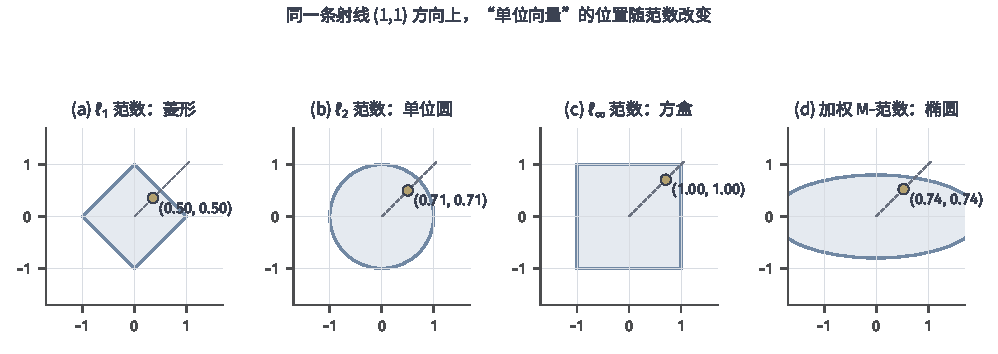
\includegraphics[width=169mm]{figures/00-shared/mathematical-preliminaries-upper/02-linear-spaces/matplotlib/ls-norm-unit-balls/ls-norm-unit-balls.pdf}
  \caption{同一向量在不同范数下的“单位球”形状。左：$\ell_1$单位球为菱形（累加绝对偏差）；中：$\ell_2$单位球为圆（欧氏长度）；右：$\ell_\infty$单位球为正方形（最大坐标偏差）。同一个点$(1,1)$的范数依次为$2$、$\sqrt2$、$1$，单位球大小随口径而变，三者之间的倍数关系将在第~\ref{sec:ls-norms-distances}节给出。三图坐标尺度相同，为解析教学例。}
  \label{fig:ls-norm-unit-balls}
\end{figure*}

本节建立了坐标向量的基本计算：加法、数乘与线性组合产生新的向量，欧氏内积把两个向量配成一个数，常用范数度量向量的大小。加法与数乘的规则将用于定义线性空间；内积与范数的一般性质留到第~\ref{chap:normed-inner-product-spaces}章。把若干向量并排放在一起，就得到下一节的矩阵。

% 第4章第2节（上）：矩阵的表示（矩阵、元素与形状，设计矩阵与贯穿例）、常见矩阵（方阵、零矩阵、对角矩阵、单位矩阵、上三角矩阵、下三角矩阵、对称矩阵、正定矩阵与半正定矩阵、置换矩阵、正交矩阵）、矩阵的运算（加法与数乘、转置、矩阵与向量的乘积、矩阵乘法、逐项乘积、逆矩阵、矩阵幂、迹、Frobenius内积、Frobenius范数、诱导矩阵范数、行列式）。运算性质随各项运算一并讨论。

\section{矩阵}
\label{sec:ls-matrices}

一批样本的特征排成一张数表以后，问题随之而来：对每个样本用同一组权重求加权和，要算许多个同样形式的和，能否一次写出；两次这样的计算接连进行，能否合成一次；一次计算能否撤销，反复进行时怎样书写；一张表把单位正方形变成平行四边形时，面积放大多少；作为计算，它最多把输入放大多少倍。这些问题都以矩阵为对象。本节先规定矩阵的写法，再介绍元素分布有固定模式的几类常见矩阵，然后逐一定义矩阵的运算，最后按运算整理它们满足的性质。

与向量不同，矩阵最重要的运算不是逐项进行的加法，而是由加权求和导出的乘法。乘法的规则与实数乘法有同有异，需要逐条核对。

\subsection{矩阵的表示与常见矩阵}
\label{sec:ls-matrix-representation}

定位向量中的一个数需要一个索引；一张数表的每个数要由所在的行与列共同确定，需要两个索引。

\paragraph{矩阵、元素与形状}
$m$行$d$列的实数表称为矩阵（matrix），记为$\bm A\in\mathbb R^{m\times d}$；第$i$行、第$j$列的元素记为$\bm A_{i,j}$，不会混淆时也写作$a_{i,j}$。$m\times d$称为矩阵的形状，行数写在列数之前。记号$\bm A_{i,:}$表示第$i$行，$\bm A_{:,j}$表示第$j$列，冒号表示该方向上的全部位置；第$j$列是一个$m$维列向量，第$i$行是一个$d$维行向量。例如在
\[
 \bm A=\begin{bmatrix}1&2&3\\4&5&6\end{bmatrix}\in\mathbb R^{2\times3}
\]
中，$\bm A_{2,1}=4$，第一行$\bm A_{1,:}=\left[\begin{smallmatrix}1&2&3\end{smallmatrix}\right]$，第三列$\bm A_{:,3}=(3,6)^\top$。

两个矩阵相等，要求形状相同且每个对应元素相等。只有一行的矩阵就是行向量，只有一列的矩阵就是列向量，所以向量可以看作矩阵的特例。

\paragraph{设计矩阵}
用矩阵记录数据时，通常让每行对应一个样本，每列对应一个特征，这样的矩阵称为设计矩阵。把示例~\ref{ex:ls-nearly-collinear-features}中两个特征的取值向量$\bm c_1,\bm c_2$并排作为两列，得到三个样本、两个特征的设计矩阵
\begin{equation}
\begin{gathered}
\bm X_{\varepsilon}
 =\begin{bmatrix}1&1\\1&1+\varepsilon\\1&1-\varepsilon\end{bmatrix}
 =\begin{bmatrix}\bm c_1&\bm c_2\end{bmatrix}\\
\bm q=\begin{bmatrix}0\\1\\-1\end{bmatrix},
 \quad \bm c_2=\bm c_1+\varepsilon\bm q.
\end{gathered}
\label{eq:linear-algebra-nearly-collinear-design}
\end{equation}
$|\varepsilon|$很小时，两列之差$\bm c_2-\bm c_1=\varepsilon\bm q$很短，两列几乎是同一串数；第~\ref{sec:ls-inner-product-definition}节将用夹角说明它们几乎同向。这个例子将贯穿整个线性空间部分：第~\ref{chap:linear-representation}章讨论这样两列能否充当一组记录方向，后面的谱与方程两章再看它怎样影响谱、求解与误差。

\subsubsection{常见矩阵}
\label{sec:prelim-common-matrices}

有些矩阵的元素分布有固定模式：大部分位置为零，或者主对角线两侧互相对称。这些模式会让后面的运算大为简化。本小节按元素的位置与取值逐类给出定义和例子；下面随各项运算讨论这些模式如何保留或改变；依赖内积的正交矩阵与正定矩阵在内积空间章建立。

\paragraph{方阵}
行数等于列数的矩阵称为方阵（square matrix），$n\times n$方阵也称$n$阶方阵；位置$(i,i)$上的元素组成主对角线。例如$\left[\begin{smallmatrix}1&2\\3&4\end{smallmatrix}\right]$是二阶方阵，主对角元素为$1$和$4$；$2\times3$矩阵不是方阵；这里讨论三角结构和对角矩阵时均限定为方阵。

\paragraph{零矩阵}
全部元素都为$0$的矩阵称为零矩阵（zero matrix），记作$\bm0$。它不要求是方阵，使用时须写明形状，例如
\[
 \bm0_{2\times3}=\begin{bmatrix}0&0&0\\0&0&0\end{bmatrix}.
\]

\paragraph{对角矩阵}
主对角线以外的元素都为$0$的方阵称为对角矩阵（diagonal matrix），记为$\operatorname{diag}(d_1,\ldots,d_n)$，主对角元素本身可以为$0$。例如
\[
\begin{gathered}
\operatorname{diag}(2,0)=\begin{bmatrix}2&0\\0&0\end{bmatrix}\\
\operatorname{diag}(1,-1,3)=\begin{bmatrix}1&0&0\\0&-1&0\\0&0&3\end{bmatrix}.
\end{gathered}
\]

\paragraph{单位矩阵}
主对角元素全为$1$的对角矩阵称为单位矩阵（identity matrix），记为$\bm I_n$，不必强调阶数时写作$\bm I$。它的第$j$列就是标准坐标向量$\bm e_j$。例如
\[
 \bm I_3=\begin{bmatrix}1&0&0\\0&1&0\\0&0&1\end{bmatrix}=\begin{bmatrix}\bm e_1&\bm e_2&\bm e_3\end{bmatrix}.
\]

\paragraph{上三角矩阵}
$i>j$时$\bm A_{i,j}=0$的方阵称为上三角矩阵（upper triangular matrix）：主对角线以下全为零，非零元素只可能出现在主对角线及其上方。例如
\[
 \begin{bmatrix}1&2&3\\0&4&5\\0&0&6\end{bmatrix}.
\]

\paragraph{下三角矩阵}
$i<j$时$\bm A_{i,j}=0$的方阵称为下三角矩阵（lower triangular matrix）：主对角线以上全为零。例如
\[
 \begin{bmatrix}1&0&0\\2&3&0\\4&5&6\end{bmatrix}.
\]
对角矩阵既是上三角矩阵，也是下三角矩阵。

\paragraph{对称矩阵}
满足$\bm A_{i,j}=\bm A_{j,i}$对全部$i,j$成立的方阵称为对称矩阵（symmetric matrix），它关于主对角线镜像对称；定义转置以后，这个条件写作$\bm A^\top=\bm A$。例如
\[
\begin{bmatrix}1&2\\2&3\end{bmatrix},\qquad
\begin{bmatrix}4&-1&0\\-1&2&5\\0&5&1\end{bmatrix}.
\]
对角矩阵都是对称矩阵。

\paragraph{置换矩阵}
把单位矩阵的各列重新排列得到的方阵称为置换矩阵（permutation matrix），它的每行、每列恰有一个$1$，其余为$0$。例如
\[
\begin{bmatrix}0&1\\1&0\end{bmatrix}=\begin{bmatrix}\bm e_2&\bm e_1\end{bmatrix},\qquad
\begin{bmatrix}0&0&1\\1&0&0\\0&1&0\end{bmatrix}=\begin{bmatrix}\bm e_2&\bm e_3&\bm e_1\end{bmatrix}.
\]
第一个矩阵乘在平面向量上会交换两个坐标，这一点在定义矩阵乘法以后验证。

\subsection{矩阵的基本运算}
\label{sec:ls-matrix-operation-properties}
\label{sec:ls-matrix-operations}
\label{sec:ls-multiplication}

矩阵的运算按来源可以分成几类。加法与数乘沿用向量的逐项规则，转置只改变元素的位置。矩阵与向量的乘积一次写出许多加权和，矩阵乘法、逆矩阵与矩阵幂都以它为基础。逐项乘积是另一种“相乘”，它不汇总任何索引。迹、行列式与矩阵范数把矩阵读成一个数，我们在下一节讨论。本节先给出运算方法，再检查它们满足的规则。

\subsubsection{加法与数乘}

同形矩阵$\bm A,\bm B\in\mathbb R^{m\times n}$逐项相加减，数乘把每个元素乘以同一个实数$c$：
\[
 \begin{gathered}
(\bm A\pm\bm B)_{i,j}=a_{i,j}\pm b_{i,j}\\
(c\bm A)_{i,j}=ca_{i,j},
 \end{gathered}
\]
结果形状不变。下面是一组二阶矩阵的算例。
\begin{example}[矩阵的加法、减法与数乘]
\label{ex:ls-matrix-addition-scaling}
给定：$\bm A=\left(\begin{smallmatrix}1&2\\3&4\end{smallmatrix}\right)$，$\bm B=\left(\begin{smallmatrix}0&1\\-1&2\end{smallmatrix}\right)$，$c=3$。
计算：逐项运算，
\[
\begin{gathered}
\bm A+\bm B=\begin{pmatrix}1&3\\2&6\end{pmatrix}\\
\bm A-\bm B=\begin{pmatrix}1&1\\4&2\end{pmatrix}\\
3\bm A=\begin{pmatrix}3&6\\9&12\end{pmatrix}.
\end{gathered}
\]
例如$\bm A+\bm B$的$(2,1)$元为$3+(-1)=2$，$\bm A-\bm B$的$(2,1)$元为$3-(-1)=4$。
结论：三个结果都是$2\times2$矩阵，每个元素只用到输入在同一位置上的元素。
\end{example}
与向量一样，两个矩阵能够相加，要求形状相同、对应位置含义相同；即使元素总数恰好相同，$2\times3$矩阵与$3\times2$矩阵也不能相加。同形矩阵的线性组合按同样方式定义。

\paragraph{加法与数乘的性质}

同形矩阵逐项相加与数乘，向量一节的八条规则在每个位置上照搬过来。对同形矩阵$\bm A,\bm B,\bm C$和实数$a,b$：
\[
\begin{aligned}
 &\bm A+\bm B=\bm B+\bm A, && (\bm A+\bm B)+\bm C=\bm A+(\bm B+\bm C),\\
 &\bm A+\bm0=\bm A, && \bm A+(-\bm A)=\bm0,\\
 &a(b\bm A)=(ab)\bm A, && 1\bm A=\bm A,\\
 &(a+b)\bm A=a\bm A+b\bm A, && a(\bm A+\bm B)=a\bm A+a\bm B.
\end{aligned}
\]
每一条都可以在任一位置$(i,j)$上用实数运算直接验证。


\subsubsection{转置}

转置交换行与列：$\bm A\in\mathbb R^{m\times n}$的元素$a_{i,j}$原样搬到$\bm A^\top\in\mathbb R^{n\times m}$的位置$(j,i)$，
\[
 (\bm A^\top)_{j,i}=\bm A_{i,j}.
\]
形状交换而数值不变，原来的第$i$行成为第$i$列。把列向量看作$d\times1$矩阵，这一定义与上一节向量的转置一致。下面的例子显示行怎样变成列。
\begin{example}[转置一个$2\times3$矩阵]
\label{ex:ls-transpose-two-by-three}
给定：$\bm A=\left[\begin{smallmatrix}1&2&3\\4&5&6\end{smallmatrix}\right]\in\mathbb R^{2\times3}$。
计算：把每个$(i,j)$元搬到$(j,i)$位置，
\[
 \bm A^\top=\begin{bmatrix}1&4\\2&5\\3&6\end{bmatrix}\in\mathbb R^{3\times2}.
\]
结论：$\bm A$的第一行$(1,2,3)$成为$\bm A^\top$的第一列，第二行$(4,5,6)$成为第二列。
\end{example}

\paragraph{转置的性质}
\label{sec:ls-reshaping}

转置改变元素的位置，也与其他矩阵运算有确定的关系。下面分别检查加法、数乘和乘积。

\paragraph{与加法、数乘交换}
\[
 \begin{gathered}
(\bm A+\bm B)^\top=\bm A^\top+\bm B^\top\\
(c\bm A)^\top=c\bm A^\top\\
(\bm A^\top)^\top=\bm A.
 \end{gathered}
\]
转置只搬动元素，逐项运算的结果搬到新位置后不变；转置两次，每个元素回到原来的位置。

\paragraph{乘积的转置}
\[
 (\bm A\bm B)^\top=\bm B^\top\bm A^\top.
\]
乘积转置后因子次序反转。按元素公式，
\[
 \begin{aligned}
 \bigl((\bm A\bm B)^\top\bigr)_{i,j}
 &=(\bm A\bm B)_{j,i}\\
 &=\sum_\ell a_{j,\ell}b_{\ell,i}\\
 &=\sum_\ell(\bm B^\top)_{i,\ell}(\bm A^\top)_{\ell,j}\\
 &=(\bm B^\top\bm A^\top)_{i,j}.
 \end{aligned}
\]
多个因子时依次使用，$(\bm A\bm B\bm C)^\top=\bm C^\top\bm B^\top\bm A^\top$。

\paragraph{内积中的转置}
\[
\langle\bm A\bm x,\bm y\rangle=\langle\bm x,\bm A^\top\bm y\rangle,\qquad
\bm A\in\mathbb R^{m\times d},\ \bm x\in\mathbb R^d,\ \bm y\in\mathbb R^m.
\]
由上一条，$(\bm A\bm x)^\top\bm y=\bm x^\top\bm A^\top\bm y$：在欧氏内积中，作用在左侧向量上的$\bm A$可以改写成作用在右侧向量上的$\bm A^\top$。

\paragraph{$\bm A^\top\bm A$对称}
对任意矩阵$\bm A$，$\bm A^\top\bm A$与$\bm A\bm A^\top$都是对称矩阵，因为$(\bm A^\top\bm A)^\top=\bm A^\top(\bm A^\top)^\top=\bm A^\top\bm A$，另一个同理。下面直接算出一个$\bm A\bm A^\top$。
\begin{example}[计算$\bm A\bm A^\top$]
\label{ex:ls-gram-product-symmetric}
给定：$\bm A=\left[\begin{smallmatrix}1&2&3\\4&5&6\end{smallmatrix}\right]$。
计算：$\bm A\bm A^\top$的$(i,j)$元是$\bm A$的第$i$行与第$j$行的内积，
\[
 \bm A\bm A^\top=\begin{bmatrix}1+4+9&4+10+18\\4+10+18&16+25+36\end{bmatrix}=\begin{bmatrix}14&32\\32&77\end{bmatrix}.
\]
结论：两个非对角元都是两行的内积$32$，结果是对称矩阵。
\end{example}

\subsubsection{矩阵与向量的乘积}
\label{sec:prelim-matrix-records-prediction}

设$n$次观测的输入排成设计矩阵$\bm X\in\mathbb R^{n\times d}$，权重排成$\bm w\in\mathbb R^d$。线性预测对每次观测计算同一种加权和$\sum_j x_{i,j}w_j$，即$\bm X$的第$i$行与$\bm w$的内积。矩阵与向量的乘积把这$n$个加权和一次写出：对$\bm A\in\mathbb R^{m\times d}$与$\bm u\in\mathbb R^d$，$\bm A\bm u$是$m$维列向量，
\begin{equation}
\begin{gathered}
(\bm A\bm u)_i=\sum_{j=1}^d\bm A_{i,j}u_j\\
i=1,\ldots,m.
\end{gathered}
\label{eq:prelim-matrix-prediction}
\end{equation}
矩阵的列数必须等于向量的维数。同一个结果有两种算法：
\begin{itemize}
 \item 按行算：输出的第$i$个坐标是第$i$行与$\bm u$的内积；
 \item 按列算：同一个$u_j$乘的恰好是第$j$列的全部元素，所以
 \[
  \bm A\bm u=u_1\bm A_{:,1}+u_2\bm A_{:,2}+\cdots+u_d\bm A_{:,d},
 \]
 乘积是矩阵各列以$u_j$为系数的线性组合。
\end{itemize}
特别地，按列算时，$\bm e_j$只有第$j$个系数为$1$，所以$\bm A\bm e_j=\bm A_{:,j}$：乘第$j$个标准坐标向量就取出第$j$列。

下面用一个二阶例子核对两种算法给出同一结果。
\begin{example}[按行与按列计算矩阵与向量的乘积]
\label{ex:ls-matrix-vector-rows-columns}
给定：$\bm A=\left[\begin{smallmatrix}2&1\\0&3\end{smallmatrix}\right]$，$\bm u=(1,1)^\top$。
计算：按行算，每个坐标是一行与$\bm u$的内积；按列算，结果是两列以$u_1=u_2=1$为系数的线性组合：
\[
\begin{gathered}
\bm A\bm u
 =\begin{bmatrix}2\cdot1+1\cdot1\\0\cdot1+3\cdot1\end{bmatrix}
 =\begin{bmatrix}3\\3\end{bmatrix}\\
\bm A\bm u=1\begin{bmatrix}2\\0\end{bmatrix}+1\begin{bmatrix}1\\3\end{bmatrix}
 =\begin{bmatrix}3\\3\end{bmatrix}.
\end{gathered}
\]
结论：两种算法都得到$\bm A\bm u=(3,3)^\top$。
\end{example}

用于数据时，矩阵与向量的乘积一次给出全部样本的预测。下面以一次函数为例。
\begin{example}[用矩阵与向量的乘积计算一次函数的取值]
\label{ex:ls-affine-predictions}
给定：要在$x=1,2,3$处计算$ax+b$，取
\[
\bm X=\begin{pmatrix}1&1\\2&1\\3&1\end{pmatrix},\qquad
\bm w=\begin{pmatrix}a\\b\end{pmatrix}.
\]
计算：按行算，
\[
 \bm X\bm w=\begin{pmatrix}1\cdot a+1\cdot b\\2\cdot a+1\cdot b\\3\cdot a+1\cdot b\end{pmatrix}=\begin{pmatrix}a+b\\2a+b\\3a+b\end{pmatrix}.
\]
结论：$\bm X\bm w$的三个坐标正是三处的函数值。第二列全为$1$，使每行都加上同一个截距$b$。
\end{example}

观测输出排成$\bm y$以后，全部残差就是$\bm X\bm w-\bm y$，平方误差总和写成
\[
 \sum_{i=1}^n\left(\sum_{j=1}^d x_{i,j}w_j-y_i\right)^2
 =\lVert\bm X\bm w-\bm y\rVert_2^2.
\]
左侧逐个样本求加权和、减去观测、平方后相加；右侧把同样的计算写成残差向量长度的平方。对贯穿例，按列算得$\bm X_\varepsilon\bm w=w_1\bm c_1+w_2\bm c_2$：预测是两个特征取值向量的线性组合。

\subsubsection{矩阵乘法}
\phantomsection
\label{sec:prelim-linear-actions-composition}

对$\bm A\in\mathbb R^{m\times d}$与$\bm B\in\mathbb R^{d\times k}$，乘积$\bm A\bm B\in\mathbb R^{m\times k}$为
\begin{equation}
 (\bm A\bm B)_{i,j}=\sum_{\ell=1}^d\bm A_{i,\ell}\bm B_{\ell,j}.
 \label{eq:prelim-matrix-composition}
\end{equation}
左矩阵的列数必须等于右矩阵的行数；第$(i,j)$项取左矩阵的第$i$行与右矩阵的第$j$列，逐项相乘后相加。下面逐项计算一个二阶乘积。
\begin{example}[二阶矩阵的乘积]
\label{ex:ls-matrix-product-2x2}
给定：$\bm A=\left(\begin{smallmatrix}1&1\\0&1\end{smallmatrix}\right)$，$\bm B=\left(\begin{smallmatrix}1&0\\0&2\end{smallmatrix}\right)$。
计算：第$(i,j)$项是$\bm A$的第$i$行与$\bm B$的第$j$列的内积，
\[
 \bm A\bm B
 =\begin{pmatrix}1\cdot1+1\cdot0&1\cdot0+1\cdot2\\0\cdot1+1\cdot0&0\cdot0+1\cdot2\end{pmatrix}
 =\begin{pmatrix}1&2\\0&2\end{pmatrix}.
\]
结论：$\bm A\bm B=\left(\begin{smallmatrix}1&2\\0&2\end{smallmatrix}\right)$，形状为$2\times2$。
\end{example}
$\bm B$只有一列时，式~\eqref{eq:prelim-matrix-composition}就是式~\eqref{eq:prelim-matrix-prediction}。两个向量的内积$\bm x^\top\bm y$是$1\times d$与$d\times1$矩阵的乘积，结果是$1\times1$矩阵，我们把它与它唯一的元素等同看待。

这个定义来自两次加权求和的接连进行。

设$\bm x\in\mathbb R^k$，$\bm y=\bm B\bm x$、$\bm z=\bm A\bm y$，即先用$\bm B$再用$\bm A$，这是第~\ref{sec:prelim-map-operations}节意义下两个函数的复合。逐坐标代入并交换有限求和的次序，
\begin{equation}
 z_i=\sum_{\ell=1}^d a_{i,\ell}y_\ell
 =\sum_{\ell=1}^d a_{i,\ell}\sum_{j=1}^k b_{\ell,j}x_j
 =\sum_{j=1}^k\left(\sum_{\ell=1}^d a_{i,\ell}b_{\ell,j}\right)x_j,
 \label{eq:linear-algebra-matrix-product}
\end{equation}
括号中的数正是$(\bm A\bm B)_{i,j}$。所以$(\bm A\bm B)\bm x=\bm A(\bm B\bm x)$：直接用乘积作用，等于先用$\bm B$、再用$\bm A$作用。被求和的公共维数$d$就是被消去的中间结果$\bm y$的维数。

非方阵相乘时，写出每个输入和输出的形状尤其有用。以$2\times3$矩阵乘$3\times2$矩阵为例，
\[
 \begin{aligned}
 &\begin{pmatrix}1&2&0\\0&1&3\end{pmatrix}
 \begin{pmatrix}1&0\\2&1\\1&-1\end{pmatrix}\\
 &=\begin{pmatrix}1\cdot1+2\cdot2+0\cdot1&1\cdot0+2\cdot1+0\cdot(-1)\\
 0\cdot1+1\cdot2+3\cdot1&0\cdot0+1\cdot1+3\cdot(-1)\end{pmatrix}\\
 &=\begin{pmatrix}5&2\\5&-2\end{pmatrix}.
 \end{aligned}
\]
两个中间维数都是$3$，因此乘法有定义；输出保留左矩阵的$2$行和右矩阵的$2$列。若把其中一个$3$改为其他数，逐项配对便无法完成。

\paragraph{乘法的性质}
矩阵乘法保留结合律和分配律，但通常不满足交换律。下面逐项核对这些规则，同时检查矩阵形状是否相容。

\paragraph{单位乘}
\[
\bm I_m\bm A=\bm A=\bm A\bm I_d,\qquad
\bm A\in\mathbb R^{m\times d}.
\]
$\bm I_m$的第$i$行是$\bm e_i^\top$，它与$\bm A$的第$j$列相乘取出$a_{i,j}$；右乘同理。单位矩阵在矩阵乘法中的作用相当于数$1$在实数乘法中的作用。

\paragraph{零乘}
\[
 \begin{gathered}
\bm0\bm A=\bm0\\
\bm A\bm0=\bm0.
 \end{gathered}
\]
乘积的每个元素都是若干乘积之和，其中一个因子全为零时，每一项都为零。这里各个零矩阵的形状由相乘的另一个因子决定。

反过来不成立：$\bm A\bm B=\bm0$不能推出$\bm A=\bm0$或$\bm B=\bm0$，下面是一个反例。
\begin{example}[反例：两个非零矩阵的乘积为零]
\label{ex:ls-zero-product-nonzero-factors}
给定：$\bm A=\left[\begin{smallmatrix}1&0\\0&0\end{smallmatrix}\right]$，$\bm B=\left[\begin{smallmatrix}0&0\\1&0\end{smallmatrix}\right]$，两者都不是零矩阵。
计算：
\[
 \bm A\bm B=\begin{bmatrix}1\cdot0+0\cdot1&1\cdot0+0\cdot0\\0\cdot0+0\cdot1&0\cdot0+0\cdot0\end{bmatrix}=\begin{bmatrix}0&0\\0&0\end{bmatrix}.
\]
结论：$\bm A\bm B=\bm0$，而$\bm A\neq\bm0$、$\bm B\neq\bm0$。
\end{example}
原因可以按列看出。由乘积的元素公式，$\bm A\bm B$的第$j$列就是$\bm A$乘$\bm B$的第$j$列，所以$\bm A\bm B=\bm0$恰好意味着$\bm B$的每一列$\bm b$都满足$\bm A\bm b=\bm0$：右因子产生的结果被左因子完全消去。上例中$\bm A$只保留第一个坐标、把第二个坐标清零，而$\bm B$的第一列$(0,1)^\top$只有第二个坐标非零，第二列为零。

\paragraph{结合律}
\[
 (\bm A\bm B)\bm C=\bm A(\bm B\bm C).
\]
按式~\eqref{eq:prelim-matrix-composition}展开，两边的第$(i,j)$项都是$\sum_k\sum_l a_{i,k}b_{k,l}c_{l,j}$，只是两个有限求和的次序不同。这也是函数复合满足结合律（第~\ref{sec:prelim-map-operations}节）在矩阵上的翻译。由结合律，多个相容矩阵连乘时不必标出括号。

\paragraph{分配律与数乘相容}
\[
 \begin{gathered}
\bm A(\bm B+\bm C)=\bm A\bm B+\bm A\bm C\\
(\bm A+\bm B)\bm C=\bm A\bm C+\bm B\bm C\\
c(\bm A\bm B)=(c\bm A)\bm B=\bm A(c\bm B),
 \end{gathered}
\]
逐项展开有限和即得。把右因子取为列向量，得到矩阵与向量的乘积对输入保持线性组合：
\begin{equation}
\bm A(a\bm u+b\bm v)=a\bm A\bm u+b\bm A\bm v,\qquad
\bm u,\bm v\in\mathbb R^d,\quad a,b\in\mathbb R.
\label{eq:prelim-matrix-linearity}
\end{equation}

由这一性质，函数$\bm u\mapsto\bm A\bm u$由它在$\bm e_1,\ldots,\bm e_d$上的输出完全确定：因为$\bm u=\sum_ju_j\bm e_j$，所以$\bm A\bm u=\sum_ju_j\bm A\bm e_j$，而这些输出$\bm A\bm e_j$就是$\bm A$的各列。第~\ref{chap:linear-representation}章把保持线性组合的函数称为线性映射，并说明每个这样的映射都能由一张矩阵记录。

\paragraph{分块乘法}
把矩阵按行、列分成尺寸相容的块，乘法规则对块照样成立：
\[
\begin{gathered}
\begin{bmatrix}\bm A&\bm B\end{bmatrix}\begin{bmatrix}\bm C\\\bm D\end{bmatrix}=\bm A\bm C+\bm B\bm D\\
\begin{bmatrix}\bm A\\\bm B\end{bmatrix}\bm C=\begin{bmatrix}\bm A\bm C\\\bm B\bm C\end{bmatrix},
\end{gathered}
\]
\[
 \bm A\begin{bmatrix}\bm C&\bm D\end{bmatrix}=\begin{bmatrix}\bm A\bm C&\bm A\bm D\end{bmatrix},
\]
以及$2\times2$分块的乘积
\[
 \begin{bmatrix}\bm A_{1,1}&\bm A_{1,2}\\\bm A_{2,1}&\bm A_{2,2}\end{bmatrix}
 \begin{bmatrix}\bm B_{1,1}&\bm B_{1,2}\\\bm B_{2,1}&\bm B_{2,2}\end{bmatrix}
 =\begin{bmatrix}
  \bm A_{1,1}\bm B_{1,1}+\bm A_{1,2}\bm B_{2,1}&\bm A_{1,1}\bm B_{1,2}+\bm A_{1,2}\bm B_{2,2}\\
  \bm A_{2,1}\bm B_{1,1}+\bm A_{2,2}\bm B_{2,1}&\bm A_{2,1}\bm B_{1,2}+\bm A_{2,2}\bm B_{2,2}
 \end{bmatrix}.
\]
条件是每个相乘的块对中，左块的列数等于右块的行数。第一式成立，是因为式~\eqref{eq:prelim-matrix-composition}对中间索引$\ell$的求和可以分段进行：前一段$\ell$对应$\bm A$的列与$\bm C$的行，后一段对应$\bm B$的列与$\bm D$的行，两段之和逐项等于整段求和。后两式只是把结果的行或列分组，$2\times2$分块由这三式合成。块可以像数一样参与运算，只是块之间的次序不能交换。

把块分到最细，得到三种常用的特例。右因子按列分块，得$(\bm A\bm B)_{:,j}=\bm A\bm B_{:,j}$：$\bm A$分别乘$\bm B$的每一列。左因子按行分块，得$(\bm A\bm B)_{i,:}=\bm A_{i,:}\bm B$：结果的第$i$行是$\bm B$各行以$\bm A_{i,:}$的元素为系数的线性组合。

第三种特例把中间维数$d$分成长度为$1$的$d$段，这时第一式给出
\begin{equation}
 \bm A\bm B=\sum_{\ell=1}^d\bm A_{:,\ell}\bm B_{\ell,:},
 \label{eq:ls-product-outer-sum}
\end{equation}
其中一列$\bm A_{:,\ell}\in\mathbb R^{m\times1}$乘一行$\bm B_{\ell,:}\in\mathbb R^{1\times k}$，得到$(i,j)$元素为$a_{i,\ell}b_{\ell,j}$的$m\times k$矩阵。式~\eqref{eq:ls-product-outer-sum}是后面低秩近似的出发点。下面用示例~\ref{ex:ls-matrix-product-2x2}的乘积核对这个公式。
\begin{example}[把乘积写成列乘行之和]
\label{ex:ls-product-as-outer-sum}
给定：示例~\ref{ex:ls-matrix-product-2x2}中的$\bm A=\left(\begin{smallmatrix}1&1\\0&1\end{smallmatrix}\right)$与$\bm B=\left(\begin{smallmatrix}1&0\\0&2\end{smallmatrix}\right)$。
计算：$\bm A$的两列为$(1,0)^\top$与$(1,1)^\top$，$\bm B$的两行为$(1,0)$与$(0,2)$，
\[
 \bm A\bm B=\begin{pmatrix}1\\0\end{pmatrix}\begin{pmatrix}1&0\end{pmatrix}+\begin{pmatrix}1\\1\end{pmatrix}\begin{pmatrix}0&2\end{pmatrix}
 =\begin{pmatrix}1&0\\0&0\end{pmatrix}+\begin{pmatrix}0&2\\0&2\end{pmatrix}=\begin{pmatrix}1&2\\0&2\end{pmatrix}.
\]
结论：两个“列乘行”矩阵之和与逐项计算的乘积相同。
\end{example}

\paragraph{交换律不成立}
一般$\bm A\bm B\neq\bm B\bm A$。形状不同时，两个乘积甚至不一定都有定义；即使两个因子是同阶方阵，两种次序的乘积也可能不同，下面是一个反例。
\begin{example}[反例：先交换再保留与先保留再交换]
\label{ex:ls-noncommuting-pair}
给定：只保留第一个坐标的$\bm P=\left[\begin{smallmatrix}1&0\\0&0\end{smallmatrix}\right]$，交换两个坐标的$\bm S=\left[\begin{smallmatrix}0&1\\1&0\end{smallmatrix}\right]$。
计算：
\[
\begin{gathered}
\bm P\bm S=\begin{bmatrix}0&1\\0&0\end{bmatrix}\\
\bm S\bm P=\begin{bmatrix}0&0\\1&0\end{bmatrix}.
\end{gathered}
\]
结论：$\bm P\bm S\neq\bm S\bm P$。作用在$\bm u\in\mathbb R^2$上，$\bm P\bm S\bm u=(u_2,0)^\top$是先交换、再保留第一个坐标，$\bm S\bm P\bm u=(0,u_1)^\top$是先保留、再交换，两种次序的结果不同。
\end{example}
书写$\bm A\bm B\bm x$时，作用顺序是从右向左：先$\bm B$，后$\bm A$。

\paragraph{消去律不成立}
$\bm A\bm B=\bm A\bm C$且$\bm A\neq\bm0$不能推出$\bm B=\bm C$。原因是$\bm A\bm B=\bm A\bm C$等价于$\bm A(\bm B-\bm C)=\bm0$，而乘积为零不能推出$\bm B-\bm C=\bm0$。下面用示例~\ref{ex:ls-zero-product-nonzero-factors}构造反例。
\begin{example}[反例：非零的左因子不能消去]
\label{ex:ls-cancellation-fails}
给定：示例~\ref{ex:ls-zero-product-nonzero-factors}中的$\bm A=\left[\begin{smallmatrix}1&0\\0&0\end{smallmatrix}\right]$与$\bm B=\left[\begin{smallmatrix}0&0\\1&0\end{smallmatrix}\right]$，以及$\bm C=\bm0$。
验证：$\bm A\bm B=\bm0=\bm A\bm C$，而$\bm B\neq\bm C$。
结论：虽然$\bm A\bm B=\bm A\bm C$且$\bm A\neq\bm0$，却不能消去$\bm A$得到$\bm B=\bm C$。
\end{example}
若$\bm A$是可逆方阵，在$\bm A\bm B=\bm A\bm C$两边左乘$\bm A^{-1}$即得$\bm B=\bm C$。所以左因子可逆时可以消去，一般的非零因子则不能。

常见矩阵参与乘法时，结果有固定模式。下面逐类给出。

\paragraph{对角矩阵的乘法}
对$\bm D=\operatorname{diag}(d_1,\ldots,d_n)$，
\[
 \begin{gathered}
(\bm D\bm A)_{i,j}=d_i\bm A_{i,j}\\
(\bm A\bm D)_{i,j}=\bm A_{i,j}d_j,
 \end{gathered}
\]
\[
 \operatorname{diag}(d_1,\ldots,d_n)\operatorname{diag}(e_1,\ldots,e_n)=\operatorname{diag}(d_1e_1,\ldots,d_ne_n).
\]
左乘对角矩阵缩放各行，右乘缩放各列：乘积公式中只有$\ell=i$（左乘时）或$\ell=j$（右乘时）的一项留下。作用在向量上，$\bm D\bm u=(d_1u_1,\ldots,d_nu_n)^\top$是逐坐标缩放。两个对角矩阵相乘时对角元逐个相乘，所以对角矩阵之间可以交换次序。下面的例子比较左乘与右乘。
\begin{example}[左乘与右乘对角矩阵]
\label{ex:ls-diagonal-scaling}
给定：$\bm D=\operatorname{diag}(2,3)$，$\bm A=\left[\begin{smallmatrix}1&2\\3&4\end{smallmatrix}\right]$。
计算：
\[
 \begin{aligned}
 \bm D\bm A&=\begin{bmatrix}2\cdot1&2\cdot2\\3\cdot3&3\cdot4\end{bmatrix}=\begin{bmatrix}2&4\\9&12\end{bmatrix},\\
 \bm A\bm D&=\begin{bmatrix}1\cdot2&2\cdot3\\3\cdot2&4\cdot3\end{bmatrix}=\begin{bmatrix}2&6\\6&12\end{bmatrix}.
 \end{aligned}
\]
结论：左乘把第一、二行分别乘以$2$、$3$，右乘把第一、二列分别乘以$2$、$3$。两个结果不同，所以对角矩阵与一般矩阵相乘时仍要区分左右。
\end{example}

\paragraph{三角矩阵的乘法}
若$\bm A,\bm B$都是$n$阶上三角矩阵，则$\bm A\bm B$也是上三角矩阵，并且
\[
 (\bm A\bm B)_{i,i}=\bm A_{i,i}\bm B_{i,i}.
\]
在$(\bm A\bm B)_{i,j}=\sum_\ell\bm A_{i,\ell}\bm B_{\ell,j}$中，$\bm A_{i,\ell}$只在$\ell\geq i$时可能非零，$\bm B_{\ell,j}$只在$\ell\leq j$时可能非零，所以只有$i\leq\ell\leq j$的项可能非零：$i>j$时没有这样的$\ell$，乘积元素为零；$i=j$时只剩$\ell=i$一项。下三角矩阵同理：两个下三角矩阵的乘积仍是下三角矩阵，对角元逐个相乘。下面是一个二阶算例。
\begin{example}[两个上三角矩阵的乘积]
\label{ex:ls-upper-triangular-product}
给定：$\bm A=\left[\begin{smallmatrix}1&2\\0&3\end{smallmatrix}\right]$，$\bm B=\left[\begin{smallmatrix}4&5\\0&6\end{smallmatrix}\right]$。
计算：
\[
 \bm A\bm B=\begin{bmatrix}1\cdot4+2\cdot0&1\cdot5+2\cdot6\\0\cdot4+3\cdot0&0\cdot5+3\cdot6\end{bmatrix}=\begin{bmatrix}4&17\\0&18\end{bmatrix}.
\]
结论：乘积仍是上三角矩阵，对角元$4=1\cdot4$、$18=3\cdot6$是两个因子对角元的乘积；右上角的$17$则同时用到了两个因子的非对角元。
\end{example}

\paragraph{置换矩阵的乘法}
设$\bm P=\left[\begin{smallmatrix}\bm e_{\sigma(1)}&\cdots&\bm e_{\sigma(n)}\end{smallmatrix}\right]$，其中$\sigma$是$\{1,\ldots,n\}$上的排列，则
\[
 \begin{gathered}
(\bm P\bm A)_{\sigma(i),:}=\bm A_{i,:}\\
(\bm A\bm P)_{:,j}=\bm A_{:,\sigma(j)}.
 \end{gathered}
\]
即左乘把$\bm A$的第$i$行移到第$\sigma(i)$行，右乘使$\bm A\bm P$的第$j$列取自$\bm A$的第$\sigma(j)$列。例如$\left[\begin{smallmatrix}0&1\\1&0\end{smallmatrix}\right]$左乘交换两行、右乘交换两列。

两个置换矩阵的乘积仍是置换矩阵：设$\bm P'$是另一个置换矩阵，$\bm P'\bm P$的第$j$列是$\bm P'\bm e_{\sigma(j)}$，即$\bm P'$的第$\sigma(j)$列；它是标准坐标向量，而且不同的$j$取到$\bm P'$的不同列，所以这些列互不相同。

\paragraph{对称矩阵的乘积}
若$\bm A,\bm B$是同阶对称矩阵，则
\[
 (\bm A\bm B)^\top=\bm B^\top\bm A^\top=\bm B\bm A,
\]
所以$\bm A\bm B$对称当且仅当$\bm A\bm B=\bm B\bm A$。对称矩阵的乘积一般不对称，下面是一个反例。
\begin{example}[反例：两个对称矩阵的乘积不对称]
\label{ex:ls-symmetric-product-not-symmetric}
给定：对称矩阵$\bm A=\left[\begin{smallmatrix}1&1\\1&0\end{smallmatrix}\right]$与$\bm B=\operatorname{diag}(1,2)$。
计算：右乘对角矩阵缩放各列，
\[
 \bm A\bm B=\begin{bmatrix}1\cdot1&1\cdot2\\1\cdot1&0\cdot2\end{bmatrix}=\begin{bmatrix}1&2\\1&0\end{bmatrix}.
\]
结论：$(\bm A\bm B)_{1,2}=2\neq1=(\bm A\bm B)_{2,1}$，乘积不对称。这与上面的判据一致：$\bm B\bm A=\left[\begin{smallmatrix}1&1\\2&0\end{smallmatrix}\right]\neq\bm A\bm B$。
\end{example}


\subsubsection{逐项乘积}
\label{sec:ls-hadamard-product}

矩阵乘法汇总共同索引；另一种常用的“乘法”不汇总任何索引，只把两个同形数组在对应位置配对。

设$\bm A,\bm B\in\mathbb R^{m\times n}$，\term{逐元素乘积}（Hadamard product）记作$\bm A\odot\bm B$，
\begin{equation}
 (\bm A\odot\bm B)_{i,j}=a_{i,j}b_{i,j},
 \label{eq:ls-hadamard}
\end{equation}
输出仍是$m\times n$。同维向量和更高阶的同形数组也按同样的方式逐项相乘。

同样两个矩阵，用两种乘法得到的结果完全不同，下面的例子说明这一点。
\begin{example}[逐项乘积与矩阵乘积的对比]
\label{ex:ls-hadamard-vs-matrix-product}
给定：$\bm A=\left[\begin{smallmatrix}1&2\\3&4\end{smallmatrix}\right]$，$\bm B=\left[\begin{smallmatrix}0&1\\1&0\end{smallmatrix}\right]$。
计算：
\[
 \begin{aligned}
 \bm A\odot\bm B&=\begin{bmatrix}1\cdot0&2\cdot1\\3\cdot1&4\cdot0\end{bmatrix}=\begin{bmatrix}0&2\\3&0\end{bmatrix},\\
 \bm A\bm B&=\begin{bmatrix}1\cdot0+2\cdot1&1\cdot1+2\cdot0\\3\cdot0+4\cdot1&3\cdot1+4\cdot0\end{bmatrix}=\begin{bmatrix}2&1\\4&3\end{bmatrix}.
 \end{aligned}
\]
结论：逐项乘积把$\bm B$为零的位置置零，矩阵乘积则交换了$\bm A$的两列；两个结果在每个位置上都不同。
\end{example}
固定掩码$\bm M$后，$\bm X\mapsto\bm M\odot\bm X$把$\bm M$为零的位置置零、把其余位置按系数缩放，适合表达“挑选或调制另一个数组”。

\paragraph{逐项乘积的性质}

逐项乘积的规则可以逐个位置从实数运算推出。以下矩阵的形状都相同。

\paragraph{交换律}
\[
 \bm A\odot\bm B=\bm B\odot\bm A.
\]
式~\eqref{eq:ls-hadamard}右端只是实数乘法，按位置逐项验证即得。逐项乘积可交换而矩阵乘积不可交换，再次说明两者是不同的运算。

\paragraph{结合律}
\[
 (\bm A\odot\bm B)\odot\bm C=\bm A\odot(\bm B\odot\bm C),
\]
两边的$(i,j)$元素都是$a_{i,j}b_{i,j}c_{i,j}$。

\paragraph{分配律}
\[
 \bm A\odot(\bm B+\bm C)=\bm A\odot\bm B+\bm A\odot\bm C,
\]
两边的$(i,j)$元素都是$a_{i,j}(b_{i,j}+c_{i,j})$。

\paragraph{单位元是全$1$数组}
全部元素为$1$的同形数组$\bm J$满足$\bm J\odot\bm A=\bm A$。单位矩阵不是逐项乘积的单位元：$\bm I_2\odot\bm A$只保留$\bm A$的对角元，把非对角元都变为零。

\paragraph{对每个因子分别线性}
固定一个因子时，$\bm X\mapsto\bm M\odot\bm X$保持线性组合。两个因子都作为未知量时，乘积只对各自分别线性：同时把两者放大两倍，结果放大四倍。第~\ref{chap:linear-representation}章换一组记录方向以后会看到，矩阵乘积对应的复合关系保持不变，逐项乘积则随记录方式改变。


\subsection{初等行变换与阶梯形}
\label{sec:ls-elementary-row-operations}

求逆时，我们需要把一个矩阵逐步化成容易辨认的形式。每一步都应当可以撤销，这样才不会丢失原矩阵中的信息。对矩阵的行允许三种\term{初等行变换}（elementary row operation）：交换两行；将一行乘以非零数；将一行加上另一行的倍数。它们的逆操作依次是再次交换同两行、乘以原系数的倒数，以及减去原来加上的倍数。

每种操作都可写成左乘一个初等矩阵：从单位矩阵出发，对其执行同样的行变换，所得矩阵记为$\bm E$，则$\bm E\bm A$恰好对$\bm A$执行该变换。例如交换两行的矩阵交换乘积的对应两行。逆操作也对应初等矩阵，因此$\bm E$可逆。

化简时从左到右寻找\term{主元}（pivot）。先在当前列尚未使用的行中找一个非零元素；若有必要，交换行把它移到当前行，再用它消去同列下方元素。若该列在余下各行全为零，就跳过这一列并继续向右。重复到没有可用行或列为止，得到的\term{行阶梯形}（row echelon form）中，零行位于底部，每个非零行的首个非零元位于上一行首个非零元的右侧。再把每个主元化为$1$，消去其上方元素，就得到\term{行最简形}（reduced row echelon form）。

处理方程$\bm A\bm x=\bm b$时，把右端项作为最后一列附在$\bm A$后面，得到增广矩阵$[\bm A\mid\bm b]$，并对整行执行同一操作。交换等式、将等式乘以非零数、把一个等式的倍数加到另一个等式，都不改变解；逆操作保证新的等式组也能还原为原等式组。下面在一个零候选主元和一列冗余的例子中逐步计算。
\begin{example}[换行、消元与自由变量]
\label{ex:ls-elementary-row-reduction}
考虑以下增广矩阵。第一列的首个元素为零，先交换前两行，再消去第三行的第一列：
\[
 \left[\begin{array}{ccc|c}0&1&2&3\\1&2&4&6\\2&4&8&12\end{array}\right]
 \longrightarrow
 \left[\begin{array}{ccc|c}1&2&4&6\\0&1&2&3\\2&4&8&12\end{array}\right]
 \longrightarrow
 \left[\begin{array}{ccc|c}1&2&4&6\\0&1&2&3\\0&0&0&0\end{array}\right].
\]
这已是阶梯形。将第一行减去第二行的两倍，得到行最简形
\[
 \left[\begin{array}{ccc|c}1&0&0&0\\0&1&2&3\\0&0&0&0\end{array}\right].
\]
第一、二列是主元列，第三列没有主元。令自由变量$x_3=t$，便读出$x_1=0$、$x_2=3-2t$；任意实数$t$都给出原方程组的一个解。最后的零行表示$0=0$，不会增加约束；若出现系数全为零而右端非零的行，则方程组无解。
\end{example}

阶梯形使主元和自由变量可见，但主元的选择会影响实际数值计算的误差。第~\ref{sec:ls-direct-methods}节会在求解方程时讨论选主元和计算代价。

\subsection{逆矩阵}
\label{sec:prelim-inverse-matrices}

对$n$阶方阵$\bm A$，若存在$n$阶方阵$\bm B$满足
\[
 \bm A\bm B=\bm B\bm A=\bm I_n,
\]
就称$\bm A$可逆，$\bm B$为\term{逆矩阵}（inverse matrix），记作$\bm A^{-1}$。逆矩阵撤销乘$\bm A$的效果。$\bm A$可逆时，若$\bm A\bm x=\bm y$，两边左乘$\bm A^{-1}$得$\bm x=\bm A^{-1}\bm y$，所以方程至多有一个解；反过来，$\bm x=\bm A^{-1}\bm y$满足$\bm A\bm x=\bm A\bm A^{-1}\bm y=\bm y$。所以方程$\bm A\bm x=\bm y$有唯一解$\bm x=\bm A^{-1}\bm y$。

逆矩阵若存在则唯一：若$\bm B,\bm C$都满足条件，则$\bm B=\bm B(\bm A\bm C)=(\bm B\bm A)\bm C=\bm C$，这里用到前面建立的结合律。因此记号$\bm A^{-1}$不会有歧义。

怎样求逆取决于矩阵的结构。下面从最简单的对角矩阵开始，依次给出二阶方阵的公式与一般方阵的做法。

\paragraph{对角矩阵的逆}
每个$d_i\neq0$时逐个取倒数：
\[
 \operatorname{diag}(d_1,\ldots,d_n)^{-1}=\operatorname{diag}(1/d_1,\ldots,1/d_n).
\]
两个对角矩阵相乘时对角元逐个相乘（前面已验证），所以两侧乘积都是$\bm I_n$。例如$\operatorname{diag}(2,1)^{-1}=\operatorname{diag}(1/2,1)$。若某个$d_i=0$，左乘$\bm D=\operatorname{diag}(d_1,\ldots,d_n)$把任何$\bm B$的第$i$行乘以$d_i$，所以$\bm D\bm B$的第$i$行是$\bm0$，不可能等于$\bm I_n$的第$i$行；这时$\bm D$不可逆。

\paragraph{二阶方阵的逆}
$ad-bc\neq0$时，
\[
 \begin{pmatrix}a&b\\c&d\end{pmatrix}^{-1}=\frac1{ad-bc}\begin{pmatrix}d&-b\\-c&a\end{pmatrix}.
\]
直接相乘即可验证两侧乘积都是$\bm I_2$：例如左上元素为$(ad-bc)/(ad-bc)=1$，右上元素为$(-ab+ba)/(ad-bc)=0$。分母$ad-bc$正是后面的二阶行列式。

\paragraph{一般方阵的逆}
一般方阵没有这样简短的公式，可以通过解方程求逆：对任意$\bm y$解$\bm A\bm x=\bm y$，把$\bm x$写成$\bm y$各坐标的线性组合，系数排成的矩阵就是$\bm A^{-1}$。下面用一个二阶例子演示，并与二阶公式对照。
\begin{example}[解方程求逆]
\label{ex:ls-inverse-by-solving}
给定：$\bm A=\left[\begin{smallmatrix}2&1\\0&3\end{smallmatrix}\right]$。
计算：方程$\bm A\bm x=\bm y$即$y_1=2x_1+x_2$、$y_2=3x_2$。由第二式得$x_2=y_2/3$，代入第一式得$x_1=(y_1-x_2)/2=y_1/2-y_2/6$。把系数排成矩阵，
\[
 \bm A^{-1}=\begin{bmatrix}1/2&-1/6\\0&1/3\end{bmatrix}.
\]
用二阶公式核对：$ad-bc=2\cdot3-1\cdot0=6$，公式给出$\frac16\left[\begin{smallmatrix}3&-1\\0&2\end{smallmatrix}\right]$，与上式相同。
结论：右上角的$-1/6$不是原元素$1$的倒数。一般矩阵把各个坐标掺在一起，逆矩阵要作为整体求出，不能逐个元素取倒数。
\end{example}
上述求法也可以用初等行变换同时处理所有右端项。把$\bm A$与单位矩阵并排，得到$[\bm A\mid\bm I_n]$，对整个增广矩阵作行变换。若左侧最终化为$\bm I_n$，这些操作合起来是某个可逆矩阵$\bm E$的左乘，于是$\bm E\bm A=\bm I_n$、右侧为$\bm E$，故$\bm E=\bm A^{-1}$。例如
\[
 \begin{aligned}
 &\left[\begin{array}{cc|cc}2&1&1&0\\0&3&0&1\end{array}\right]\\
 &\longrightarrow
 \left[\begin{array}{cc|cc}1&1/2&1/2&0\\0&1&0&1/3\end{array}\right]\\
 &\longrightarrow
 \left[\begin{array}{cc|cc}1&0&1/2&-1/6\\0&1&0&1/3\end{array}\right],
 \end{aligned}
\]
右半部分与前面的逆矩阵相同。如果方阵化简后不能在每列找到主元，左侧出现零行；由于所有行变换都可逆，这样的矩阵不能有逆。计算方程的解时，通常直接对右端项消元，不必先求出整个逆矩阵。哪些方阵可逆，第~\ref{sec:ls-injective-surjective-invertible}节用零空间与秩回答，第~\ref{sec:ls-determinant-invertibility}节再给出行列式判据。

\paragraph{单侧逆}
矩形矩阵不能有双侧的逆，但可能只从一侧抵消。对$\bm A\in\mathbb R^{m\times d}$，满足$\bm L\bm A=\bm I_d$的$\bm L\in\mathbb R^{d\times m}$称为左逆，满足$\bm A\bm R=\bm I_m$的$\bm R\in\mathbb R^{d\times m}$称为右逆。有左逆时，若$\bm A\bm x=\bm y$有解，两边左乘$\bm L$得$\bm x=\bm L\bm y$，所以解只能是$\bm L\bm y$。有右逆时，$\bm A(\bm R\bm y)=\bm I_m\bm y=\bm y$，所以$\bm x=\bm R\bm y$总是一个解。

与方阵的逆不同，单侧逆一般不唯一，下面的例子说明这一点。
\begin{example}[反例：左逆不唯一]
\label{ex:ls-left-inverse-not-unique}
给定：$\bm A=(1,0)^\top\in\mathbb R^{2\times1}$，以及任意实数$c$。
验证：取$\bm L=(1,c)\in\mathbb R^{1\times2}$，则$\bm L\bm A=1\cdot1+c\cdot0=1=\bm I_1$。
结论：每个$c$都给出$\bm A$的一个左逆，所以$\bm A$的左逆有无穷多个。
\end{example}
矩形矩阵何时有左逆或右逆，第~\ref{chap:linear-representation}章用核与像回答；第~\ref{chap:linear-equations-and-optimization}章讨论怎样实际求解，以及多解时选哪一个。

设下面的$\bm A,\bm B$都是$n$阶可逆方阵。

\paragraph{乘积的逆}
\begin{equation}
 (\bm A\bm B)^{-1}=\bm B^{-1}\bm A^{-1}.
 \label{eq:ls-inverse-product}
\end{equation}
先作用的后撤销，就像先穿袜子再穿鞋，脱的时候要先脱鞋。验证：$(\bm A\bm B)(\bm B^{-1}\bm A^{-1})=\bm A(\bm B\bm B^{-1})\bm A^{-1}=\bm A\bm A^{-1}=\bm I_n$，反方向$(\bm B^{-1}\bm A^{-1})(\bm A\bm B)=\bm I_n$同理。

\paragraph{逆的逆}
\[
 (\bm A^{-1})^{-1}=\bm A.
\]
定义中$\bm A$与$\bm A^{-1}$的地位对称：$\bm A^{-1}\bm A=\bm A\bm A^{-1}=\bm I_n$同样说明$\bm A$是$\bm A^{-1}$的逆。

\paragraph{数乘的逆}
\[
 (c\bm A)^{-1}=c^{-1}\bm A^{-1}\qquad(c\neq0).
\]
直接相乘：$(c\bm A)(c^{-1}\bm A^{-1})=(cc^{-1})\bm A\bm A^{-1}=\bm I_n$，反方向同理。

\paragraph{转置的逆}
\[
 (\bm A^\top)^{-1}=(\bm A^{-1})^\top.
\]
由乘积的转置，$\bm A^\top(\bm A^{-1})^\top=(\bm A^{-1}\bm A)^\top=\bm I^\top=\bm I$，反方向同理，所以$(\bm A^{-1})^\top$就是$\bm A^\top$的逆。

\subsection{矩阵的幂}
\label{sec:ls-matrix-power-rules}

定常迭代$\bm x^{(k+1)}=\bm A\bm x^{(k)}$每一步都乘同一个$\bm A$。对$d$阶方阵，$\bm A^k$定义为$k$个$\bm A$连乘（$k\geq1$），并规定$\bm A^0=\bm I_d$；$\bm A$可逆时再定义负幂$\bm A^{-k}=(\bm A^{-1})^k$。于是迭代的第$k$步是$\bm x^{(k)}=\bm A^k\bm x^{(0)}$。非方阵不能与自身相乘，所以没有矩阵幂。

幂是反复的矩阵乘法，不是逐元素乘方，下面的例子说明两者的差别。
\begin{example}[矩阵的平方不是逐元素平方]
\label{ex:ls-matrix-square-shear}
给定：$\bm A=\left(\begin{smallmatrix}1&1\\0&1\end{smallmatrix}\right)$。
计算：
\[
 \bm A^2=\begin{pmatrix}1&1\\0&1\end{pmatrix}\begin{pmatrix}1&1\\0&1\end{pmatrix}
 =\begin{pmatrix}1\cdot1+1\cdot0&1\cdot1+1\cdot1\\0\cdot1+1\cdot0&0\cdot1+1\cdot1\end{pmatrix}
 =\begin{pmatrix}1&2\\0&1\end{pmatrix}.
\]
结论：右上角的元素变为$2$，而逐元素平方会得到$1^2=1$；继续相乘，右上角每次增加$1$。
\end{example}

同一矩阵的整数幂按结合律满足$\bm A^r\bm A^s=\bm A^{r+s}$和$(\bm A^r)^s=\bm A^{rs}$；出现负指数时要求$\bm A$可逆。但不同矩阵不一定交换，因此
\[
 (\bm A+\bm B)^2=\bm A^2+\bm A\bm B+\bm B\bm A+\bm B^2,
\]
只有$\bm A\bm B=\bm B\bm A$时才能将中间两项合成$2\bm A\bm B$。这与标量平方公式的差别来自乘法次序。

两类幂关系经常出现。满足$\bm A^2=\bm A$的方阵称为\term{幂等}（idempotent）矩阵，乘一次与乘多次效果相同。存在正整数$s$使$\bm N^s=\bm0$的方阵称为\term{幂零}（nilpotent）矩阵。下面各举一例。
\begin{example}[幂等矩阵与幂零矩阵]
\label{ex:ls-idempotent-nilpotent}
给定：$\bm P=\operatorname{diag}(1,0)$，$\bm N=\left(\begin{smallmatrix}0&1\\0&0\end{smallmatrix}\right)$。
计算：对$\bm u\in\mathbb R^2$，$\bm P\bm u=(u_1,0)^\top$只保留第一个坐标，再作用一次结果不变，所以$\bm P^2=\bm P$。$\bm N\bm u=(u_2,0)^\top$把第二个坐标移到第一个位置、把第二个位置清零；再作用一次得$\bm N(u_2,0)^\top=(0,0)^\top$。直接相乘也得到
\[
 \bm N^2=\begin{pmatrix}0&1\\0&0\end{pmatrix}\begin{pmatrix}0&1\\0&0\end{pmatrix}=\begin{pmatrix}0&0\\0&0\end{pmatrix}.
\]
结论：$\bm P$是幂等矩阵；$\bm N\neq\bm0$，却满足$\bm N^2=\bm0$，是幂零矩阵。
\end{example}
$\bm A^k$在$k$很大时是什么样子，很难从元素看出，第~\ref{chap:linear-analysis}章借助特征向量回答。

\paragraph{幂的性质}

设$\bm A$为方阵，$m,n$为非负整数；$\bm A$可逆时，$m,n$可取任意整数。

\paragraph{同底幂相乘}
\[
 \bm A^m\bm A^n=\bm A^{m+n}.
\]
由结合律，两边都是同样个数的$\bm A$（或$\bm A^{-1}$）连乘；指数异号时，相邻的$\bm A\bm A^{-1}$逐对消去。交换$m,n$的角色可见，同一矩阵的不同次幂彼此可以交换。

\paragraph{幂的幂}
\[
 (\bm A^m)^n=\bm A^{mn}.
\]
左边是$n$组、每组$m$个因子的连乘，由结合律去掉括号即得。

\paragraph{负幂与逆相容}
\[
 (\bm A^k)^{-1}=(\bm A^{-1})^k=\bm A^{-k}.
\]
对$k$个相同因子反复使用式~\eqref{eq:ls-inverse-product}即得。

% 方阵和同形矩阵的标量读数：行列式、迹与元素内积。
\section{行列式、迹与元素内积}
\label{sec:ls-matrix-scalar-readouts}

矩阵运算可以产生另一张数表，也可以产生一个标量。行列式衡量方阵作用下有向体积的缩放；迹累计主对角元素；Frobenius内积比较同形矩阵的全部对应元素。它们回答的问题不同，不能只凭其中一个数恢复原矩阵。

\subsection{行列式的定义与计算}
\phantomsection
\label{sec:ls-exterior-determinants}
\label{sec:linear-algebra-scalar-readouts}

一张方阵把单位正方形变成平行四边形、把单位立方体变成平行多面体时，面积或体积放大多少倍？平行四边形的面积不能由两条边的长度直接算出，它还取决于两个向量的相对方向；若再记录定向，交换两个向量的次序会使有向面积变号。下面先建立记录有向体积的外积，再由它得到行列式和它的计算公式。

\paragraph{外积}
对$\mathbb R^d$中的$k$个向量$\bm v_1,\ldots,\bm v_k$，它们的\term{外积}（exterior product，又称\term{楔积}wedge product）$\bm v_1\wedge\cdots\wedge\bm v_k$按两条规则计算。
\begin{itemize}
 \item 多线性：对每个因子分别保持线性组合，即把某个$\bm v_i$换成$a\bm u+b\bm w$时，整个楔积等于$a(\cdots\wedge\bm u\wedge\cdots)+b(\cdots\wedge\bm w\wedge\cdots)$，其余因子不动。
 \item 交替性：交换相邻两个因子，楔积变号，
 \[
  \cdots\wedge\bm v_i\wedge\bm v_j\wedge\cdots
  =-\cdots\wedge\bm v_j\wedge\bm v_i\wedge\cdots.
 \]
\end{itemize}

两条规则先给出两个推论。第一，含有两个相同因子的楔积为零：两个相同因子相邻时，交换它们不改变楔积，却使它变号，所以它等于自身的相反数，只能为零；两个相同因子不相邻时，先用相邻交换把它们移到一起，只改变符号，结论不变。第二，若某个因子是其余因子的线性组合，把这个因子按组合代入并由多线性展开，每一项都含有两个相同因子，所以整个楔积为零。

由此可以确定楔积的一般形状。

设$v_{j,i}$是$\bm v_j$的第$i$个坐标，把每个$\bm v_j=\sum_i v_{j,i}\bm e_i$代入并展开，含重复下标的项为零；其余各项按交替性把下标排成递增次序，只改变符号。所以每个楔积都是基楔积$\bm e_{i_1}\wedge\cdots\wedge\bm e_{i_k}$（$i_1<\cdots<i_k$）的线性组合，这样的基楔积共有$\binom{d}{k}$个。$k>d$时，每一项都必然含有重复下标，所以楔积恒为零。

对$\{1,\ldots,k\}$上的一般排列$\pi$，可以反复交换相邻的两个因子，把$\bm v_{\pi(1)}\wedge\cdots\wedge\bm v_{\pi(k)}$排回$\bm v_1\wedge\cdots\wedge\bm v_k$。记$N(\pi)$为$\pi$的逆序对数，即满足$i<j$而$\pi(i)>\pi(j)$的索引对数。每次交换一对相邻且次序颠倒的因子，逆序对数恰好减少$1$，所以恰好经过$N(\pi)$次交换就排好，每次交换变号一次，得到
\[
 \begin{gathered}
\bm v_{\pi(1)}\wedge\cdots\wedge\bm v_{\pi(k)}
 =\operatorname{sgn}(\pi)\,\bm v_1\wedge\cdots\wedge\bm v_k\\
\operatorname{sgn}(\pi)=(-1)^{N(\pi)}.
 \end{gathered}
\]

\paragraph{有向面积与有向体积}
在$\mathbb R^2$中按两条规则展开，
\[
 \bm u\wedge\bm v
 =(u_1\bm e_1+u_2\bm e_2)\wedge(v_1\bm e_1+v_2\bm e_2)
 =(u_1v_2-u_2v_1)\,\bm e_1\wedge\bm e_2,
\]
其中用到$\bm e_1\wedge\bm e_1=\bm e_2\wedge\bm e_2=0$与$\bm e_2\wedge\bm e_1=-\bm e_1\wedge\bm e_2$。系数$u_1v_2-u_2v_1$是$\bm u,\bm v$张成的平行四边形的有向面积：绝对值是面积，符号是定向。

下面用三组向量观察有向面积的数值与符号。
\begin{example}[平面上的有向面积]
\label{ex:ls-oriented-area}
给定：三组有序向量对：$\bm u=(1,0)^\top$与$\bm v=(1,1)^\top$；交换次序后的$\bm v$与$\bm u$；共线的$(1,1)^\top$与$(2,2)^\top$。
计算：按系数公式$u_1v_2-u_2v_1$，三组依次得到
\[
 \begin{gathered}
1\cdot1-0\cdot1=1\\
1\cdot0-1\cdot1=-1\\
1\cdot2-1\cdot2=0.
 \end{gathered}
\]
结论：第一组张成面积为$1$的平行四边形；交换次序后面积不变而定向翻转，所以符号变负；共线的两个向量张成的平行四边形退化成线段，有向面积为$0$。
\end{example}
由上面的计数，$\mathbb R^3$中三个向量的楔积只是基楔积$\bm e_1\wedge\bm e_2\wedge\bm e_3$的倍数。这个系数的绝对值是三个向量张成的平行六面体的体积，带符号时称为\term{有向体积}。

\paragraph{行列式的定义}
在$\mathbb R^d$中取$d$个向量，最高阶楔积只剩一个基楔积$\bm e_1\wedge\cdots\wedge\bm e_d$。对$d$阶方阵$\bm A$，把它的各列$\bm A\bm e_1,\ldots,\bm A\bm e_d$作楔积，
\[
 \bm A\bm e_1\wedge\cdots\wedge\bm A\bm e_d
 =(\det\bm A)\,\bm e_1\wedge\cdots\wedge\bm e_d,
\]
标量$\det\bm A$称为\term{行列式}（determinant）。它是$\bm A$把单位立方体变成平行多面体时的有向体积倍数，绝对值为体积比，符号表示定向是否翻转。图~\ref{fig:ls-determinant-oriented-volume}在平面上画出这一缩放。
\begin{figure*}[htbp]
  \centering
  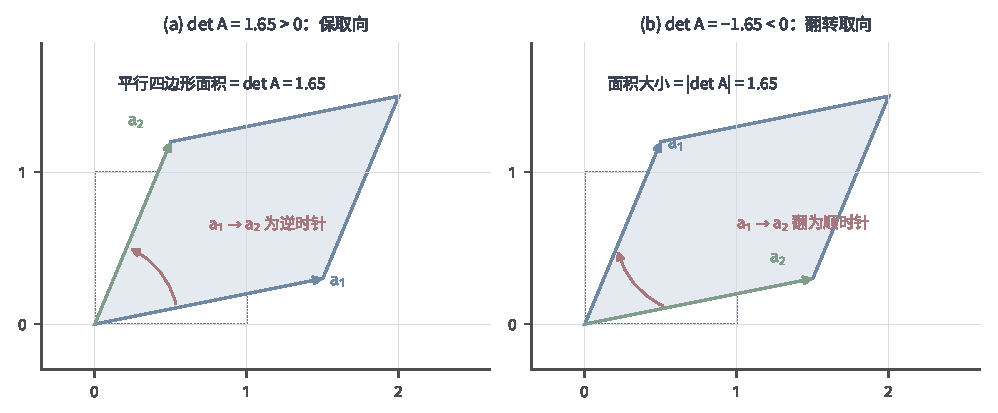
\includegraphics[width=169mm]{figures/00-shared/mathematical-preliminaries-upper/02-linear-spaces/matplotlib/ls-determinant-oriented-volume/ls-determinant-oriented-volume.pdf}
  \caption{行列式作为有向体积的缩放。左：单位正方形由$\bm e_1=(1,0)$、$\bm e_2=(0,1)$张成，面积为$1$。中：$\bm A=\bigl(\begin{smallmatrix}2&0.5\\0&1.5\end{smallmatrix}\bigr)$把它映成由$\bm A\bm e_1=(2,0)$、$\bm A\bm e_2=(0.5,1.5)$张成的平行四边形，有向面积为$2\cdot1.5-0.5\cdot0=3=\det\bm A>0$（保定向）。右：$\bm A$把$\bm e_1$反射到$(-2,0)$，有向面积为$-3$（反定向）。向量与数值均为解析教学例。}
  \label{fig:ls-determinant-oriented-volume}
\end{figure*}

\paragraph{排列展开}
把$\bm A\bm e_j=\sum_i a_{i,j}\bm e_i$代入楔积并展开。若第$j$个因子选出$\bm e_{\tau(j)}$，得到的项为$\bigl(\prod_ja_{\tau(j),j}\bigr)\,\bm e_{\tau(1)}\wedge\cdots\wedge\bm e_{\tau(d)}$。下标有重复的项为零；留下的项中$\tau$是$\{1,\ldots,d\}$的一个排列，而$\bm e_{\tau(1)}\wedge\cdots\wedge\bm e_{\tau(d)}=\operatorname{sgn}(\tau)\,\bm e_1\wedge\cdots\wedge\bm e_d$。所以
\[
 \det\bm A=\sum_{\tau}\operatorname{sgn}(\tau)\prod_{j=1}^d a_{\tau(j),j},
\]
求和遍历全部排列。习惯上按行书写：记$\pi=\tau^{-1}$，把乘积按行号重排，得到$\prod_ia_{i,\pi(i)}$。$\tau$的逆序对$(i,j)$与$\pi$的逆序对$(\tau(j),\tau(i))$一一对应，所以$\operatorname{sgn}(\pi)=\operatorname{sgn}(\tau)$。于是得到计算公式
\[
 \det\bm A
 =\sum_{\pi\in S_d}\operatorname{sgn}(\pi)
   \prod_{i=1}^d a_{i,\pi(i)},
\]
其中$S_d$是$\{1,\ldots,d\}$到自身的全部双射，每个$\pi$规定第$i$行选取第$\pi(i)$列。计算步骤是：对每个排列，从每行各取一个元素、各列恰好取一次，把取出的$d$个数相乘，再按逆序对数的奇偶加上正负号求和。

二阶时只有两个排列：恒等排列没有逆序对，取正号；交换$1,2$的排列有一个逆序对，取负号。于是
\[
 \det\begin{pmatrix}a&b\\c&d\end{pmatrix}=ad-bc,
\]
例如$\det\left(\begin{smallmatrix}1&2\\3&4\end{smallmatrix}\right)=1\cdot4-2\cdot3=-2$。

三阶时有六个排列。恒等排列与两个循环排列$(\pi(1),\pi(2),\pi(3))=(2,3,1)$、$(3,1,2)$的逆序对数为$0$或$2$，取正号；只交换两个位置的三个排列$(1,3,2)$、$(2,1,3)$、$(3,2,1)$的逆序对数为$1$或$3$，取负号。于是
\[
 \begin{aligned}
 \det\bm A={}&a_{1,1}a_{2,2}a_{3,3}+a_{1,2}a_{2,3}a_{3,1}+a_{1,3}a_{2,1}a_{3,2}\\
 &-a_{1,1}a_{2,3}a_{3,2}-a_{1,2}a_{2,1}a_{3,3}-a_{1,3}a_{2,2}a_{3,1}.
 \end{aligned}
\]
下面用这个公式计算一个具体的三阶行列式。
\begin{example}[三阶行列式的排列展开]
\label{ex:ls-det-three-by-three}
给定：$\bm A=\left(\begin{smallmatrix}2&0&1\\1&3&0\\0&1&1\end{smallmatrix}\right)$。
计算：按上式的六项次序代入，
\[
 \begin{aligned}
 \det\bm A&=2\cdot3\cdot1+0\cdot0\cdot0+1\cdot1\cdot1-2\cdot0\cdot1-0\cdot1\cdot1-1\cdot3\cdot0\\
 &=6+0+1-0-0-0=7.
 \end{aligned}
\]
结论：$\det\bm A=7$。六项中只有两项非零，其余四项都含有零元素。
\end{example}

行列式因而是矩阵元素的多项式。上面的推导只说明：若楔积满足两条规则，行列式只能是这个和。反过来可以直接验证，排列展开式作为各列的函数确实对每列线性、交换两列时变号（交换两列相当于把每个$\pi$复合上一次对换，逆序对数的奇偶随之改变），并且在单位矩阵处等于$1$。所以两条规则彼此相容，行列式由它们和$\det\bm I_d=1$唯一确定。高阶时排列有$d!$个，实际计算通常利用下面的性质和消元。



\subsection{行列式的性质与可逆性}
\label{sec:ls-determinant-properties}
\phantomsection
\label{sec:prelim-determinants}

行列式由楔积的两条规则定义，下面前两条性质就是这两条规则在列上的表述，其余性质由它们推出。

设$\bm A,\bm B$为$d$阶方阵。

\paragraph{对列的多线性}
\[
 \det\begin{bmatrix}\cdots&a\bm u+b\bm w&\cdots\end{bmatrix}
 =a\det\begin{bmatrix}\cdots&\bm u&\cdots\end{bmatrix}
 +b\det\begin{bmatrix}\cdots&\bm w&\cdots\end{bmatrix},
\]
其中三个矩阵只在同一列不同，其余各列相同。$\det\bm A$是各列楔积的系数，所以这正是楔积对每个因子保持线性组合的直接翻译。

\paragraph{交替性}
交换两列，行列式变号；两列相同，行列式为零。前者来自楔积交换两个因子时变号（不相邻的两个因子可以经奇数次相邻交换互换位置）；后者是因为交换两个相同的列不改变矩阵，行列式却要变号，只能为零。

两条合起来又得到两个常用推论。把某列的倍数加到另一列上，行列式不变：按多线性拆开，多出的一项含两列相同，为零。某一列是其余各列的线性组合时，行列式为零：把这一列按组合展开，每一项都含两列相同。例如$\det\left(\begin{smallmatrix}1&2\\2&4\end{smallmatrix}\right)=4-4=0$，第二列是第一列的$2$倍。

\paragraph{转置不变}
\[
 \det(\bm A^\top)=\det\bm A.
\]
在排列展开中，把每一项的乘积按列号重排，得$\prod_ia_{i,\pi(i)}=\prod_ja_{\pi^{-1}(j),j}$；排列展开的推导已经说明$\operatorname{sgn}(\pi^{-1})=\operatorname{sgn}(\pi)$。$\pi$遍历$S_d$时，$\sigma=\pi^{-1}$也遍历$S_d$，所以
\[
 \det\bm A=\sum_{\sigma\in S_d}\operatorname{sgn}(\sigma)\prod_{j=1}^da_{\sigma(j),j}
 =\sum_{\sigma\in S_d}\operatorname{sgn}(\sigma)\prod_{j=1}^d(\bm A^\top)_{j,\sigma(j)}
 =\det(\bm A^\top).
\]
于是对列成立的多线性与交替性，对行同样成立。

\paragraph{行变换与可逆性}
行上的多线性和交替性给出三条计算规则：交换两行使行列式变号；某行乘以非零数$c$使行列式乘以$c$；某行加上另一行的倍数不改变行列式。第三条是因为按该行展开后，多出的矩阵有两行相同，其行列式为零。

用这些规则配合消元，可以把方阵化为上三角矩阵，再取对角元素的乘积并补偿换行及倍乘的影响。例如
\[
 \det\begin{pmatrix}0&1&2\\1&2&1\\2&7&4\end{pmatrix}
 =-\det\begin{pmatrix}1&2&1\\0&1&2\\0&3&2\end{pmatrix}
 =-\det\begin{pmatrix}1&2&1\\0&1&2\\0&0&-4\end{pmatrix}=4.
\]
第一步交换前两行，并从第三行减去第一行的两倍；第二步再从第三行减去第二行的三倍。交换行使符号改变，两次加倍数不改变行列式。

这也把行列式与求逆联系起来。消元中的每一步都可逆，而且只使行列式乘以一个非零数。

若每列都找到主元，阶梯形是对角元非零的上三角矩阵，故行列式非零，并可继续化为单位矩阵求逆。

若某列找不到主元，方阵的阶梯形至少有一行全零，行列式为零，也无法化为单位矩阵。因此方阵可逆当且仅当其行列式非零。

\paragraph{数乘与加法}
\[
\begin{gathered}
\det(c\bm A)=c^d\det\bm A\\
\det(\bm A+\bm B)\neq\det\bm A+\det\bm B\ (\text{一般}).
\end{gathered}
\]
数乘把$d$列各乘以$c$，由对每列的线性提出$d$个$c$。行列式只对每一列分别线性，对整个矩阵却不是线性的，下面是一个反例。
\begin{example}[反例：行列式不保持加法]
\label{ex:ls-det-not-additive}
给定：$\bm A=\bm B=\bm I_2$。
计算：$\det\bm A+\det\bm B=1+1=2$，而由第一式，$\det(\bm A+\bm B)=\det(2\bm I_2)=2^2\det\bm I_2=4$。
结论：$\det(\bm A+\bm B)\neq\det\bm A+\det\bm B$。
\end{example}

\paragraph{乘法性}
\[
 \det(\bm A\bm B)=\det\bm A\,\det\bm B.
\]
接连作用两次时，体积缩放倍数应当相乘。排列展开的推导只用到楔积的两条规则，所以把$\bm e_1,\ldots,\bm e_d$换成任意向量$\bm w_1,\ldots,\bm w_d$，同样有$\bigwedge_j\bigl(\sum_ib_{i,j}\bm w_i\bigr)=(\det\bm B)\,\bm w_1\wedge\cdots\wedge\bm w_d$。由$(\bm A\bm B)\bm e_j=\bm A(\bm B\bm e_j)=\sum_i b_{i,j}\bm A\bm e_i$，取$\bm w_i=\bm A\bm e_i$，得到
\[
 (\bm A\bm B)\bm e_1\wedge\cdots\wedge(\bm A\bm B)\bm e_d
 =(\det\bm B)\,\bm A\bm e_1\wedge\cdots\wedge\bm A\bm e_d
 =(\det\bm A)(\det\bm B)\,\bm e_1\wedge\cdots\wedge\bm e_d.
\]
尽管矩阵乘法不可交换，$\det(\bm A\bm B)=\det(\bm B\bm A)$总成立，因为两边都等于$\det\bm A\,\det\bm B$。

\paragraph{三角矩阵的行列式}
\[
 \det\bm A=a_{1,1}a_{2,2}\cdots a_{d,d}\qquad(\bm A\text{为上三角或下三角矩阵}).
\]
设$\bm A$为上三角矩阵。排列$\pi$不是恒等排列时，必有某行$i$满足$\pi(i)<i$（因为$\sum_i(\pi(i)-i)=0$而各项不全为零），这一行选到主对角线下方的零元素，所以这一项为零；排列展开中只剩恒等排列一项。下三角时同理。例如$\det\left(\begin{smallmatrix}1&2&3\\0&4&5\\0&0&6\end{smallmatrix}\right)=1\cdot4\cdot6=24$；特别地，$\det\operatorname{diag}(d_1,\ldots,d_d)=d_1\cdots d_d$，$\det\bm I=1$。与乘法性合起来，两个上三角矩阵乘积的行列式就是两者全部对角元之积，这与三角矩阵乘积的对角元逐个相乘一致。

\paragraph{按行（列）展开}
对$d\geq2$，删除第$i$行、第$j$列得到的$(d-1)$阶子矩阵记为$\bm A^{(i,j)}$，定义\term{代数余子式}（cofactor）
\[
 C_{i,j}=(-1)^{i+j}\det\bm A^{(i,j)}.
\]
则对任一行$i$与任一列$j$，
\[
 \det\bm A=\sum_{j=1}^d a_{i,j}C_{i,j}=\sum_{i=1}^d a_{i,j}C_{i,j}.
\]
把排列展开按第$i$行选取的列分类，选第$j$列的各项之和正是$a_{i,j}C_{i,j}$；按列同理。下面沿第一行展开示例~\ref{ex:ls-det-three-by-three}中的矩阵，与排列展开的结果对照。
\begin{example}[沿第一行展开三阶行列式]
\label{ex:ls-det-cofactor-expansion}
给定：$\bm A=\left(\begin{smallmatrix}2&0&1\\1&3&0\\0&1&1\end{smallmatrix}\right)$。
计算：第一行元素为$2,0,1$，对应代数余子式的符号依次为$+,-,+$，
\[
 \begin{aligned}
 \det\bm A
 &=2\cdot\det\begin{pmatrix}3&0\\1&1\end{pmatrix}
 -0\cdot\det\begin{pmatrix}1&0\\0&1\end{pmatrix}
 +1\cdot\det\begin{pmatrix}1&3\\0&1\end{pmatrix}\\
 &=2\cdot3-0\cdot1+1\cdot1=7.
 \end{aligned}
\]
结论：结果与示例~\ref{ex:ls-det-three-by-three}的排列展开一致。
\end{example}

\paragraph{古典伴随恒等式}
把全部代数余子式排成矩阵$\bm C$，其转置称为\term{古典伴随}（classical adjugate）$\operatorname{adj}(\bm A)=\bm C^\top$。
\begin{theorem}[古典伴随恒等式]
\label{thm:ls-adjugate-identity}
对任意$d$阶方阵$\bm A$，
\[
 \bm A\,\operatorname{adj}(\bm A)
 =\operatorname{adj}(\bm A)\,\bm A
 =(\det\bm A)\,\bm I_d.
\]
\end{theorem}
\begin{proof}
乘积$\bm A\bm C^\top$的$(i,k)$元素为$\sum_j a_{i,j}C_{k,j}$。当$i=k$时，这正是沿第$i$行展开的$\det\bm A$。当$i\neq k$时，$C_{k,j}$不涉及第$k$行的元素，所以这个和是把第$k$行换成第$i$行后的矩阵沿第$k$行的展开；新矩阵有两行相同，行列式为零。于是$\bm A\bm C^\top=(\det\bm A)\bm I_d$。按列展开同样得到$\bm C^\top\bm A=(\det\bm A)\bm I_d$。
\end{proof}
二阶时$\operatorname{adj}\left(\begin{smallmatrix}a&b\\c&d\end{smallmatrix}\right)=\left(\begin{smallmatrix}d&-b\\-c&a\end{smallmatrix}\right)$，恒等式两边除以$ad-bc$就是第~\ref{sec:prelim-inverse-matrices}节的二阶求逆公式。

古典伴随是由余子式得到的代数构造，与第~\ref{sec:ls-inner-product-spaces}节由内积配对定义的伴随不是同一个对象。高阶时展开余子式的代价是阶乘级的，所以恒等式主要作为证明工具：下面用它证明方阵的单侧逆即逆，第~\ref{sec:ls-determinant-invertibility}节用它给出可逆判据，第~\ref{sec:ls-characteristic-polynomial}节用它证明Cayley--Hamilton定理。

\paragraph{方阵的单侧逆即逆}
\phantomsection
\label{sec:ls-square-one-sided-inverse}
若$n$阶方阵满足$\bm B\bm A=\bm I_n$或$\bm A\bm B=\bm I_n$，则$\bm A$可逆且$\bm B=\bm A^{-1}$。

由乘法性，两种情形都有$\det\bm A\det\bm B=\det\bm I_n=1$，所以$\det\bm A\neq0$。令$\bm C=\operatorname{adj}(\bm A)/\det\bm A$，古典伴随恒等式给出$\bm A\bm C=\bm C\bm A=\bm I_n$，所以$\bm A$可逆，$\bm C=\bm A^{-1}$。若$\bm B\bm A=\bm I_n$，则$\bm B=\bm B(\bm A\bm C)=(\bm B\bm A)\bm C=\bm C$；若$\bm A\bm B=\bm I_n$，则$\bm B=(\bm C\bm A)\bm B=\bm C(\bm A\bm B)=\bm C$。所以检查方阵的逆只需验证一侧的乘积。对矩形矩阵，左逆与右逆则可以只存在一个，也可以不唯一（示例~\ref{ex:ls-left-inverse-not-unique}）。

\subsection{迹}
\label{sec:prelim-matrix-trace}

$n$阶方阵的\term{迹}（trace）是主对角元素之和：
\[
 \operatorname{tr}(\bm A)=\sum_{i=1}^n A_{i,i}.
\]
例如$\operatorname{tr}\left(\begin{smallmatrix}1&2\\3&4\end{smallmatrix}\right)=1+4=5$，而这个矩阵全部元素之和是$10$。迹只对方阵定义，只累加对角元。


\subsubsection{迹的性质}
\phantomsection
\label{sec:ls-matrix-contractions}

\paragraph{线性}
\[
 \operatorname{tr}(a\bm A+b\bm B)=a\operatorname{tr}(\bm A)+b\operatorname{tr}(\bm B),
\]
这是有限和的线性。

\paragraph{转置不变}
\[
 \operatorname{tr}(\bm A^\top)=\operatorname{tr}(\bm A),
\]
因为转置不改变对角元。

\paragraph{循环性}
对$\bm A\in\mathbb R^{m\times n}$、$\bm B\in\mathbb R^{n\times m}$，
\begin{equation}
 \operatorname{tr}(\bm A\bm B)
 =\sum_{i=1}^m\sum_{j=1}^n A_{i,j}B_{j,i}
 =\operatorname{tr}(\bm B\bm A).
 \label{eq:linear-algebra-trace-cyclic}
\end{equation}
两个双重和只是求和次序不同。$\bm A\bm B$与$\bm B\bm A$可以是不同阶的方阵，相等的是迹，不是矩阵本身，下面的例子说明这一点。
\begin{example}[不同阶乘积的迹相等]
\label{ex:ls-trace-cyclic-different-sizes}
给定：$\bm A=\left[\begin{smallmatrix}1&2&3\end{smallmatrix}\right]\in\mathbb R^{1\times3}$，$\bm B=(1,0,2)^\top\in\mathbb R^{3\times1}$。
计算：$\bm A\bm B=1\cdot1+2\cdot0+3\cdot2=7$是$1\times1$矩阵；
\[
 \bm B\bm A=\begin{bmatrix}1&2&3\\0&0&0\\2&4&6\end{bmatrix}
\]
是$3\times3$矩阵，对角元为$1,0,6$。
结论：$\operatorname{tr}(\bm A\bm B)=7=1+0+6=\operatorname{tr}(\bm B\bm A)$，而两个乘积的阶数不同。
\end{example}

三个因子时，循环性只允许把因子整体循环移动：
\[
 \operatorname{tr}(\bm A\bm B\bm C)=\operatorname{tr}(\bm B\bm C\bm A)=\operatorname{tr}(\bm C\bm A\bm B).
\]
第一个等号把$\bm A$与$\bm B\bm C$看作两个因子使用式~\eqref{eq:linear-algebra-trace-cyclic}，第二个等号把$\bm A\bm B$与$\bm C$看作两个因子。任意交换相邻因子则可能改变迹，下面是一个反例。
\begin{example}[反例：交换相邻因子会改变迹]
\label{ex:ls-trace-adjacent-swap}
给定：$\bm A=\left(\begin{smallmatrix}1&0\\0&0\end{smallmatrix}\right)$，$\bm B=\left(\begin{smallmatrix}0&0\\1&0\end{smallmatrix}\right)$，$\bm C=\left(\begin{smallmatrix}0&1\\0&0\end{smallmatrix}\right)$。
计算：$\bm A\bm B=\bm0$，所以$\bm A\bm B\bm C=\bm0$。另一方面$\bm A\bm C=\bm C$，所以
\[
 \bm A\bm C\bm B=\begin{pmatrix}0&1\\0&0\end{pmatrix}\begin{pmatrix}0&0\\1&0\end{pmatrix}=\begin{pmatrix}1&0\\0&0\end{pmatrix}.
\]
结论：$\operatorname{tr}(\bm A\bm B\bm C)=0$，而$\operatorname{tr}(\bm A\bm C\bm B)=1$；交换$\bm B$与$\bm C$的次序改变了迹。
\end{example}


\subsection{矩阵的元素内积}
\subsubsection{Frobenius内积}

把同形矩阵的$mn$个元素看作有限个坐标，照搬欧氏内积，就得到同形矩阵之间的\term{Frobenius内积}：对$\bm A,\bm B\in\mathbb R^{m\times n}$，
\[
 \langle\bm A,\bm B\rangle_{\mathrm F}=\sum_{i=1}^m\sum_{j=1}^na_{i,j}b_{i,j},
\]
即逐项相乘后全部相加，也就是$\bm A\odot\bm B$全部元素之和。下面沿用逐项乘积一例中的两个矩阵。
\begin{example}[Frobenius内积的计算]
\label{ex:ls-frobenius-inner-product}
给定：$\bm A=\left(\begin{smallmatrix}1&2\\3&4\end{smallmatrix}\right)$，$\bm B=\left(\begin{smallmatrix}0&1\\1&0\end{smallmatrix}\right)$。
计算：
\[
 \langle\bm A,\bm B\rangle_{\mathrm F}=1\cdot0+2\cdot1+3\cdot1+4\cdot0=5.
\]
结论：结果等于示例~\ref{ex:ls-hadamard-vs-matrix-product}中$\bm A\odot\bm B$的元素之和$0+2+3+0=5$。
\end{example}

\paragraph{Frobenius内积的迹表示}
\[
 \begin{gathered}
 \langle\bm A,\bm B\rangle_{\mathrm F}=\operatorname{tr}(\bm A^\top\bm B),\\
 \lVert\bm A\rVert_{\mathrm F}^2=\operatorname{tr}(\bm A^\top\bm A).
 \end{gathered}
\]
$\bm A^\top\bm B$的第$j$个对角元为$\sum_i A_{i,j}B_{i,j}$，再对$j$求和恰好遍历所有位置。反过来，计算$\operatorname{tr}(\bm A\bm B)$时也不必形成乘积：只需算$\sum_{i,j}A_{i,j}B_{j,i}$，代价为$mn$次乘法，而形成整个$\bm A\bm B$需要$m^2n$次。



\subsubsection{Frobenius范数}
\label{sec:ls-frobenius-norm}

矩阵的“大小”有两种口径。第一种把矩阵当作数表，由Frobenius内积给出Frobenius范数
\[
 \lVert\bm A\rVert_{\mathrm F}=\sqrt{\langle\bm A,\bm A\rangle_{\mathrm F}}=\left(\sum_{i,j}a_{i,j}^2\right)^{1/2}.
\]
例如$\lVert\left(\begin{smallmatrix}1&2\\3&4\end{smallmatrix}\right)\rVert_{\mathrm F}=\sqrt{1+4+9+16}=\sqrt{30}$。它就是把$mn$个元素排成一列以后的$2$范数，其范数性质将在第~\ref{sec:ls-normed-space-definition}节由Minkowski不等式统一验证。

Frobenius范数也可以按作用来读。由$\bm A\bm e_j=\bm A_{:,j}$，
\[
 \lVert\bm A\rVert_{\mathrm F}^2=\sum_j\lVert\bm A_{:,j}\rVert_2^2=\sum_j\lVert\bm A\bm e_j\rVert_2^2,
\]
它是全部标准坐标输入所产生的输出平方和，而不是某一个最坏输入的放大。

需要先分组再汇总时，还可以用混合范数，例如以行为组的$\lVert\bm A\rVert_{p,q}=(\sum_i\lVert\bm A_{i,:}\rVert_p^q)^{1/q}$：内层的$p$范数衡量每组的大小，外层的$q$范数汇总各组。

% 第4章第3节：张量的表示（多维数组、轴、阶、形状、切片）、张量的运算（轴置换、形状重整与向量化、张量积、Kronecker积、张量缩约）、张量运算的性质（重排的性质、张量积的性质、Kronecker积的性质、缩约的性质、各种乘积的形状）。

\section{张量}
\label{sec:ls-tensors-objects}

一批图像要记录样本、通道和两个像素坐标，一批文本要记录样本、位置和特征维度：定位其中一个数需要三个甚至更多的索引，一张二维数表装不下。程序里常把这样的数组换轴、拉平或改变形状，这样做以后哪些量不变？两个向量的全部两两乘积怎样组织，两个矩阵分别作用在不同的轴上时怎样合写，一个多轴数组又怎样沿指定的轴汇总成低阶数组？本节先给出多维数组的记法，再逐一定义轴置换、形状重整、张量积、Kronecker积与缩约，最后按运算整理它们的性质，并说明前两节的内积、矩阵乘法与迹都是缩约的特例。

\subsection{张量的表示}
\label{sec:ls-tensor-representation}

向量用一个索引定位一个数，矩阵用两个。当一个量由多路索引共同决定时，需要更多索引。机器学习中常把这样的多索引数值数组称为\term{张量}（tensor）。
\begin{definition}[多维数值数组]
\label{def:linear-algebra-multidimensional-array}
给定正整数$n_1,\ldots,n_k$，形状为$n_1\times\cdots\times n_k$的数值数组，是从$\{1,\ldots,n_1\}\times\cdots\times\{1,\ldots,n_k\}$到$\mathbb R$的映射。第$j$个索引称为第$j$个\term{轴}（axis），轴数$k$称为数组的\term{阶}（order）。
\end{definition}
按这一说法，向量、矩阵分别是一阶、二阶数组，并约定单个标量是零阶数组。阶是索引的个数，形状记录各轴的长度；单个轴的长度不是阶，$\mathbb R^{100}$中的向量仍是一阶数组。

例如$\bm X\in\mathbb R^{b\times\ell\times d}$可以记录$b$个样本、每个样本$\ell$个位置、每个位置$d$个特征，$x_{i,j,k}$由三个索引共同定位。固定部分索引得到切片：$\bm X_{i,:,:}$保留第$i$个样本，是一个$\ell\times d$矩阵；$\bm X_{i,j,:}$再固定位置，是一个$d$维向量。图~\ref{fig:ls-scalar-vector-matrix-tensor}按“定位一个数需要几个索引”把四类数组并排比较。
\begin{figure}[!htb]
  \centering
  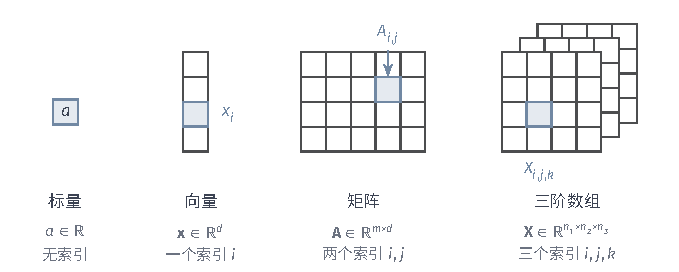
\includegraphics[width=112mm]{figures/00-shared/mathematical-preliminaries-upper/02-linear-spaces/tikz/comprehension-additions/scalar-vector-matrix-tensor.pdf}
  \caption{标量、向量、矩阵与三阶数组的区别。每个面板用蓝色标出一个数：标量本身就是这个数，向量用一个索引$i$定位，矩阵用行列两个索引$i,j$定位，三阶数组再加一个索引$k$选择切片。索引个数称为阶，各轴长度组成形状。}
  \label{fig:ls-scalar-vector-matrix-tensor}
\end{figure}

两个同形数组按位置逐项相加、数乘，规则与向量、矩阵完全相同；两个数组能否相加，仍要求形状相同、对应轴的含义相同。使用多维数组时，须先说清每条轴记录什么：同一个$b\times\ell\times d$数组，若把第二、三轴的含义弄反，后续的每一次汇总都会汇总错的轴。

\subsection{张量的运算}
\label{sec:ls-tensor-operations}

多轴数组的运算按对轴的作用分成三类。轴置换与形状重整只改变元素记录在哪条轴、哪个位置上，不改变数值，也不求和。张量积和它的矩阵形式Kronecker积把多个因子的轴全部保留下来，组合成轴更多的数组。缩约则反过来，指定一对或几对轴对齐相乘后求和，把数组汇总成更低阶的数组。

\subsubsection{轴置换}
\label{sec:ls-tensor-reshaping}
\phantomsection
\label{sec:linear-algebra-tensors-structured-operations}

\term{维度重排}（permutation of axes）按给定顺序调换轴的位置，元素跟随自己的索引移动。计算时先写出新旧索引的对应，再按对应搬运元素。例如把$\bm X\in\mathbb R^{b\times\ell\times d}$的第二、三轴互换，得到$\bm Y\in\mathbb R^{b\times d\times\ell}$，
\[
 y_{i,k,j}=x_{i,j,k}.
\]
第一个轴保持原位，每个样本的切片被转置：$\bm Y_{i,:,:}=(\bm X_{i,:,:})^\top$。下面取一个具体的小数组。
\begin{example}[交换后两条轴]
\label{ex:ls-axis-swap}
给定：$b=1$、$\ell=2$、$d=3$，唯一的样本切片为$\bm X_{1,:,:}=\left[\begin{smallmatrix}1&2&3\\4&5&6\end{smallmatrix}\right]$。
计算：按$y_{1,k,j}=x_{1,j,k}$搬运元素，例如$y_{1,3,2}=x_{1,2,3}=6$，得到
\[
 \bm Y_{1,:,:}=\begin{bmatrix}1&4\\2&5\\3&6\end{bmatrix}.
\]
结论：$\bm Y\in\mathbb R^{1\times3\times2}$，它的样本切片正是原切片的转置。
\end{example}
矩阵的转置是两个轴时唯一的非平凡轴置换。轴的含义跟着轴走，不因位置改变而改变：$\bm Y$的第二轴仍是特征，第三轴仍是位置。

\subsubsection{形状重整与向量化}

\term{形状重整}（reshape）先按指定的遍历顺序把全部元素读成一个数列，再把这个数列按同样的顺序装入另一形状；它只要求元素总数相同。计算分两步：读出、装入。下面的例子比较按行重整与转置。
\begin{example}[按行重整与转置的区别]
\label{ex:ls-reshape-vs-transpose}
给定：$\bm A=\left[\begin{smallmatrix}1&2&3\\4&5&6\end{smallmatrix}\right]$，目标形状为$3\times2$。
计算：按行读出得数列$1,2,3,4,5,6$，再按行装入$3\times2$数组，得到
\[
 \bm R=\begin{bmatrix}1&2\\3&4\\5&6\end{bmatrix},
 \qquad\text{而}\qquad
 \bm A^\top=\begin{bmatrix}1&4\\2&5\\3&6\end{bmatrix}.
\]
结论：$\bm R$与$\bm A^\top$形状相同、所含的数相同，排列却不同。
\end{example}
所以重整不能只给目标形状，还要给遍历顺序；形状相同也不能说明完成了轴交换。图~\ref{fig:vol1-add-linear-transpose-reshape}把两种结果并排放置。
\begin{figure}[!htb]
  \centering
  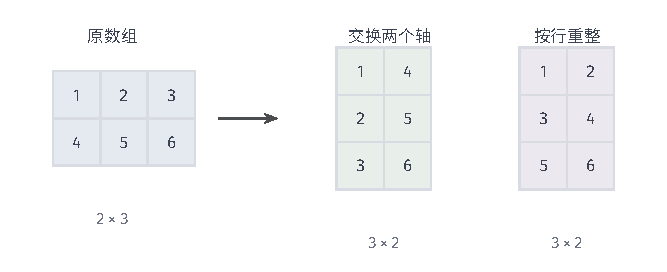
\includegraphics[width=112mm]{figures/00-shared/mathematical-preliminaries-upper/02-linear-spaces/tikz/comprehension-additions/linear-transpose-reshape.pdf}
  \caption{轴交换与按行重整。原数组两行为$(1,2,3)$与$(4,5,6)$；中图转置后两列分别保留原来的两行，右图则把按行读取的数列$1,2,3,4,5,6$依次装入$3\times2$数组。数字及其排列由正文示例直接给出。}
  \label{fig:vol1-add-linear-transpose-reshape}
\end{figure}

形状重整中最常用的一种，是把矩阵按列堆叠成一个长列向量，称为\term{向量化}（vectorization）：
\[
 \operatorname{vec}(\bm A)=(a_{1,1},\ldots,a_{m,1},a_{1,2},\ldots,a_{m,2},\ldots,a_{1,n},\ldots,a_{m,n})^\top,
\]
$m\times n$矩阵的元素$a_{i,j}$位于一维索引$i+(j-1)m$。例如上面的$\bm A$给出$\operatorname{vec}(\bm A)=(1,4,2,5,3,6)^\top$，其中$a_{2,3}=6$位于第$2+(3-1)\cdot2=6$个位置。

多维数组也可以按轴重整成矩阵，称为矩阵展开（unfolding）：把一部分轴合并成行索引，其余轴合并成列索引。例如把$\bm X\in\mathbb R^{b\times\ell\times d}$的前两轴合并为行，得到$b\ell\times d$矩阵，每行是一个样本在一个位置上的特征。选哪些轴合并，决定展开结果的形状，也决定后续乘积汇总哪个轴。

\subsubsection{张量积}
\label{sec:ls-tensor-products}
\phantomsection
\label{sec:linear-algebra-joint-operations}

两个向量的全部两两乘积排成一个数组，就是它们的张量积。设$\bm x\in\mathbb R^m$、$\bm y\in\mathbb R^n$，\term{张量积}（tensor product）$\bm x\otimes\bm y$是$m\times n$数组，
\[
 (\bm x\otimes\bm y)_{i,j}=x_i y_j.
\]
写成矩阵，$\bm x\otimes\bm y=\bm x\bm y^\top$，正是分块乘法式~\eqref{eq:ls-product-outer-sum}中“一列乘一行”的矩阵。每个因子各占结果的一条轴，下面称为一个槽位。三个向量的张量积$(\bm x\otimes\bm y\otimes\bm z)_{i,j,k}=x_i y_j z_k$保留三个槽位，多重张量积按同样规则逐槽位相乘。下面计算两个二维向量的张量积。
\begin{example}[两个二维向量的张量积]
\label{ex:ls-tensor-product-two-vectors}
给定：$\bm x=(1,2)^\top$，$\bm y=(3,-1)^\top$。
计算：
\[
 \bm x\otimes\bm y=\begin{pmatrix}1\cdot3&1\cdot(-1)\\2\cdot3&2\cdot(-1)\end{pmatrix}=\begin{pmatrix}3&-1\\6&-2\end{pmatrix}.
\]
结论：第$i$行是$x_i\bm y^\top$，所以每一行都是$\bm y^\top$的倍数；同理，每一列都是$\bm x$的倍数。
\end{example}
图~\ref{fig:ls-tensor-product-slots}展示张量积怎样保留两个因子的槽位。
\begin{figure}[htbp]
  \centering
  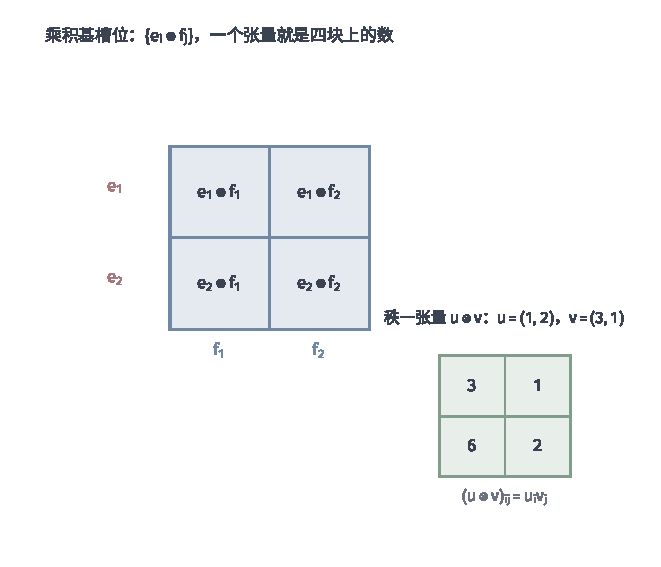
\includegraphics[width=112mm]{figures/00-shared/mathematical-preliminaries-upper/02-linear-spaces/matplotlib/ls-tensor-product-slots/ls-tensor-product-slots.pdf}
  \caption{张量积并排保留两个因子的槽位。左：$\bm u\in\mathbb R^2$、$\bm v\in\mathbb R^3$。右：$\bm u\otimes\bm v$排成$2\times3$网格，每行由$\bm v$方向复制并按$u_i$缩放；它是简单张量，数值由$\bm u=(1,0.6)$、$\bm v=(1,0.5,0.2)$直接相乘得到，是教学构造。}
  \label{fig:ls-tensor-product-slots}
\end{figure}

形如$\bm x\otimes\bm y$的数组称为\term{简单张量}（simple tensor）。由示例~\ref{ex:ls-tensor-product-two-vectors}的结论，简单张量的各行都是同一个向量的倍数。并非每个二阶数组都是简单张量，下面是一个反例。
\begin{example}[反例：单位矩阵不是简单张量]
\label{ex:ls-identity-not-simple}
给定：$\bm I_2$，它的两行为$(1,0)$与$(0,1)$。
验证：若$\bm I_2=\bm x\otimes\bm y$，则两行分别是$x_1\bm y^\top$与$x_2\bm y^\top$。两行都非零，所以$x_1,x_2\neq0$，两行都是$\bm y^\top$的非零倍数，从而彼此成比例。但$(1,0)$与$(0,1)$不成比例。
结论：$\bm I_2$不能写成任何$\bm x\otimes\bm y$，它不是简单张量。
\end{example}
不过，每个$m\times n$数组$\bm T$都是简单张量的和，
\[
 \bm T=\sum_{i,j}t_{i,j}\,\bm e_i\otimes\bm f_j,
\]
其中$\bm e_i$、$\bm f_j$分别是$\mathbb R^m$与$\mathbb R^n$的标准坐标向量，$\bm e_i\otimes\bm f_j$只在位置$(i,j)$为$1$。

张量积的用处，是把同时依赖两组输入的读取化为对单个数组的线性读取。设实值函数$B(\bm x,\bm y)$对$\bm x$、$\bm y$分别保持线性组合（称为双线性）。把$\bm x=\sum_ix_i\bm e_i$、$\bm y=\sum_jy_j\bm f_j$代入，按两次线性展开，
\[
 B(\bm x,\bm y)=\sum_{i,j}x_iy_j\,B(\bm e_i,\bm f_j)=\sum_{i,j}g_{i,j}(\bm x\otimes\bm y)_{i,j}
 =\langle\bm G,\bm x\otimes\bm y\rangle_{\mathrm F},
\]
其中$g_{i,j}=B(\bm e_i,\bm f_j)$。所以双线性读取由一张固定的系数表$\bm G$决定，并且它对数组$\bm x\otimes\bm y$是线性的。以欧氏内积$B(\bm x,\bm y)=\bm x^\top\bm y$（$m=n$）为例，$g_{i,j}=\langle\bm e_i,\bm e_j\rangle$，即$\bm G=\bm I$，读取就是把$\bm x\otimes\bm y$的对角线加起来。

二阶张量与矩阵是同一组数的两种记录：张量强调槽位来自哪一组输入，矩阵强调行列在乘法中的角色。

\subsubsection{Kronecker积}

两个矩阵分别作用在两条轴上时，联合作用可以写成一张大矩阵。对$\bm A\in\mathbb R^{m\times n}$、$\bm B\in\mathbb R^{p\times q}$，定义Kronecker积
\begin{equation}
 \bm A\otimes\bm B
 =\begin{bmatrix}
  A_{1,1}\bm B&\cdots&A_{1,n}\bm B\\
  \vdots&\ddots&\vdots\\
  A_{m,1}\bm B&\cdots&A_{m,n}\bm B
 \end{bmatrix}\in\mathbb R^{mp\times nq}.
 \label{eq:linear-algebra-kronecker-product}
\end{equation}
计算时把$\bm A$的每个元素$A_{i,j}$替换成块$A_{i,j}\bm B$。下面计算一个二阶的例子。
\begin{example}[两个二阶矩阵的Kronecker积]
\label{ex:ls-kronecker-two-by-two}
给定：$\bm A=\left[\begin{smallmatrix}1&2\\3&4\end{smallmatrix}\right]$，$\bm B=\left[\begin{smallmatrix}0&1\\1&0\end{smallmatrix}\right]$。
计算：
\[
 \bm A\otimes\bm B
 =\begin{bmatrix}
  1\cdot\bm B&2\cdot\bm B\\
  3\cdot\bm B&4\cdot\bm B
 \end{bmatrix}
 =\begin{bmatrix}0&1&0&2\\1&0&2&0\\0&3&0&4\\3&0&4&0\end{bmatrix}.
\]
结论：$\bm A\otimes\bm B$是$4\times4$矩阵，四个$2\times2$块依次是$\bm B$的$1,2,3,4$倍。
\end{example}
图~\ref{fig:ls-kronecker-block-structure}用另一组数展示这种逐元素替换的分块结构。
\begin{figure}[htbp]
  \centering
  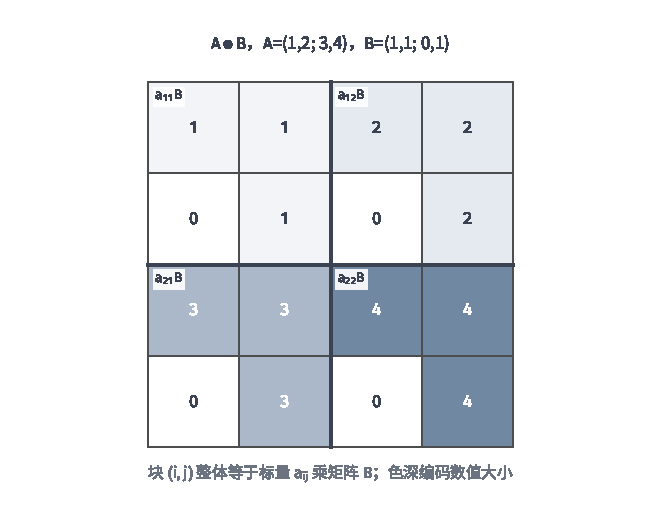
\includegraphics[width=112mm]{figures/00-shared/mathematical-preliminaries-upper/02-linear-spaces/matplotlib/ls-kronecker-block-structure/ls-kronecker-block-structure.pdf}
  \caption{Kronecker积的分块结构。上：$\bm A=\bigl(\begin{smallmatrix}1&2\\3&4\end{smallmatrix}\bigr)$、$\bm B=\bigl(\begin{smallmatrix}10&20\\30&40\end{smallmatrix}\bigr)$。下：$\bm A\otimes\bm B$是把$\bm A$的每个元素替换为该元素乘$\bm B$得到的$4\times4$分块矩阵，块边界用白线强调。数值由定义直接计算，是教学例。}
  \label{fig:ls-kronecker-block-structure}
\end{figure}

两个列向量按式~\eqref{eq:linear-algebra-kronecker-product}相乘，得到$mn$维长向量$(x_1\bm y^\top,\ldots,x_m\bm y^\top)^\top$，它正是把$m\times n$数组$\bm x\otimes\bm y$按行读出的结果。两种用法记录的是同一组数，只差一次按行读出，所以同一个记号$\otimes$不会引起混淆。例如$(1,2)^\top\otimes(3,-1)^\top=(3,-1,6,-2)^\top$，与示例~\ref{ex:ls-tensor-product-two-vectors}中的数组按行读出的结果相同。

\subsubsection{张量缩约}
\label{sec:ls-tensor-contraction}

张量积把槽位全部保留；缩约则沿指定的轴汇总。计算时选定一对或几对尺寸相同的轴，让每对轴共用同一个求和索引，逐项相乘后对这些索引求和；被求和的轴消失，其余轴保留，按原次序组成输出的形状。写出索引，就能检查哪些轴被消去、哪些轴应当保留，下面用两个例子说明这种检查。
\begin{example}[两种缩约的输出形状]
\label{ex:ls-contraction-shapes}
给定：（1）$\bm A\in\mathbb R^{m\times d\times r}$与$\bm B\in\mathbb R^{d\times n\times r}$；（2）$\bm X\in\mathbb R^{b\times\ell\times d}$与$\bm W\in\mathbb R^{d\times h}$。
计算：（1）让$\bm A$的第二轴与$\bm B$的第一轴共用索引$k$，两者的第三轴共用索引$s$，
\[
 c_{i,j}=\sum_{k=1}^d\sum_{s=1}^r a_{i,k,s}b_{k,j,s}.
\]
（2）让$\bm X$的最后一轴与$\bm W$的第一轴共用索引$k$，
\[
 z_{i,j,t}=\sum_{k=1}^d x_{i,j,k}w_{k,t}.
\]
结论：（1）同时消去$k$与$s$两对轴，保留$i,j$，输出为$m\times n$矩阵。（2）只消去$k$，保留$i,j,t$，输出形状为$b\times\ell\times h$：每个样本、每个位置上的$d$维特征都乘了同一个矩阵$\bm W$。
\end{example}
图~\ref{fig:ls-tensor-contraction}沿一对选中的轴求和并保留其余轴。
\begin{figure}[htbp]
  \centering
  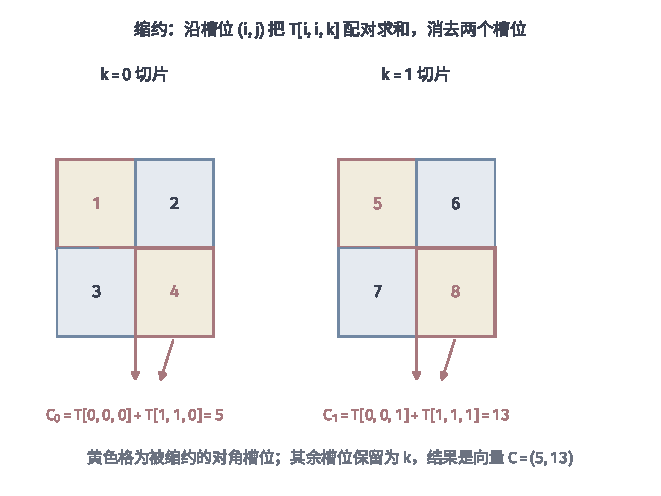
\includegraphics[width=112mm]{figures/00-shared/mathematical-preliminaries-upper/02-linear-spaces/matplotlib/ls-tensor-contraction/ls-tensor-contraction.pdf}
  \caption{张量缩约沿选中的一对轴求和、保留其余轴。左：二阶张量按行和列着色；选中列轴（虚线箭头）沿列求和，输出对每行汇总为一个值。右：缩约后得到$3$个输出，分别对应原矩阵三行的行和，颜色由红（小）经黄到蓝（大）。张量与数值均为解析教学例。}
  \label{fig:ls-tensor-contraction}
\end{figure}

前两节的几种运算都是缩约：
\begin{itemize}
 \item 内积$\sum_jx_jy_j$缩约两个向量唯一的一对轴，输出标量；
 \item 矩阵乘法$\sum_\ell a_{i,\ell}b_{\ell,j}$只消去左因子的列轴与右因子的行轴这一对；
 \item 迹$\sum_iA_{i,i}$把同一个矩阵的行轴与列轴对齐到同一索引后求和；
 \item Frobenius内积$\sum_{i,j}a_{i,j}b_{i,j}$同时缩约两对轴。
\end{itemize}

\subsection{张量运算的性质}
\label{sec:ls-tensor-operation-properties}

使用上一小节的运算时，须知道哪些操作可以撤销、括号怎样移动、Kronecker积怎样与普通矩阵乘法配合，以及缩约何时可以分开计算。本小节按运算整理，最后用一张表汇总各种“乘法”的形状条件。

\subsubsection{重排的性质}

\paragraph{可逆性}
目标形状与遍历顺序固定后，轴置换、形状重整与向量化都把一个数组一一对应到另一个数组，逆操作恢复原数组：转置再转置、按逆置换换回、按原顺序装回。例如$\operatorname{vec}$的逆操作把长度为$mn$的向量依次每$m$个一列装回$m\times n$矩阵。所以重排保留全部信息。

\paragraph{线性}
\[
 \operatorname{vec}(a\bm A+b\bm B)=a\operatorname{vec}(\bm A)+b\operatorname{vec}(\bm B),
\]
轴置换与形状重整同样满足这一性质：它们只搬动元素，逐项的加法与数乘搬到新位置后不变。

\paragraph{与矩阵乘法的关系}
转置与乘法有整齐的规则$(\bm A\bm B)^\top=\bm B^\top\bm A^\top$；一般的形状重整与乘法没有这样的关系。重整以后，矩阵每一行、每一列汇集的元素都变了，依赖行列结构的乘积、迹与行列式一般随之改变。下面的反例把示例~\ref{ex:ls-reshape-vs-transpose}中的$\bm R$误当作$\bm A^\top$使用。
\begin{example}[反例：重整不能代替转置]
\label{ex:ls-reshape-breaks-product}
给定：$\bm A=\left[\begin{smallmatrix}1&2&3\\4&5&6\end{smallmatrix}\right]$，以及按行重整得到的$\bm R=\left[\begin{smallmatrix}1&2\\3&4\\5&6\end{smallmatrix}\right]$。
计算：由示例~\ref{ex:ls-gram-product-symmetric}，$\bm A\bm A^\top=\left[\begin{smallmatrix}14&32\\32&77\end{smallmatrix}\right]$；而
\[
 \bm A\bm R=\begin{bmatrix}1+6+15&2+8+18\\4+15+30&8+20+36\end{bmatrix}=\begin{bmatrix}22&28\\49&64\end{bmatrix}.
\]
结论：$\bm R$与$\bm A^\top$形状相同、所含的数相同，两个乘积的迹却分别为$14+77=91$与$22+64=86$。
\end{example}
把存储格式的改变当成计算效果，是这里最常见的错误。

\subsubsection{张量积的性质}

\paragraph{对每个因子线性}
\[
 (a\bm x)\otimes\bm y=\bm x\otimes(a\bm y)=a(\bm x\otimes\bm y),\qquad
 (\bm x+\bm x')\otimes\bm y=\bm x\otimes\bm y+\bm x'\otimes\bm y,
\]
对第二个因子的加法同样分配。每个元素$x_iy_j$对$x_i$和$y_j$分别线性，逐项验证即得。

\paragraph{结合律}
\[
 (\bm x\otimes\bm y)\otimes\bm z=\bm x\otimes(\bm y\otimes\bm z),
\]
两边的$(i,j,k)$元素都是$x_iy_jz_k$。

\paragraph{交换槽位是转置}
\[
 \bm y\otimes\bm x=(\bm x\otimes\bm y)^\top,
\]
因为$\bm x\otimes\bm y$的$(i,j)$元素$x_iy_j$也是$\bm y\otimes\bm x$的$(j,i)$元素。所以一般$\bm x\otimes\bm y\neq\bm y\otimes\bm x$，两者相差一次轴置换。

\paragraph{Frobenius配对与范数分离}
\[
 \langle\bm x\otimes\bm y,\bm x'\otimes\bm y'\rangle_{\mathrm F}
 =\langle\bm x,\bm x'\rangle\langle\bm y,\bm y'\rangle,
 \qquad
 \lVert\bm x\otimes\bm y\rVert_{\mathrm F}=\lVert\bm x\rVert_2\,\lVert\bm y\rVert_2.
\]
第一式来自$\sum_{i,j}x_iy_jx'_iy'_j=(\sum_ix_ix'_i)(\sum_jy_jy'_j)$；第二式在第一式中取$\bm x'=\bm x$、$\bm y'=\bm y$后开平方。下面在示例~\ref{ex:ls-tensor-product-two-vectors}的数组上核对第二式。
\begin{example}[张量积范数的数值核对]
\label{ex:ls-tensor-product-norm-check}
给定：$\bm x=(1,2)^\top$，$\bm y=(3,-1)^\top$，$\bm x\otimes\bm y=\left(\begin{smallmatrix}3&-1\\6&-2\end{smallmatrix}\right)$。
计算：$\lVert\bm x\rVert_2=\sqrt5$，$\lVert\bm y\rVert_2=\sqrt{10}$；直接求Frobenius范数，
\[
 \lVert\bm x\otimes\bm y\rVert_{\mathrm F}=\sqrt{3^2+(-1)^2+6^2+(-2)^2}=\sqrt{50}.
\]
结论：$\sqrt5\cdot\sqrt{10}=\sqrt{50}=5\sqrt2$，两种算法一致。
\end{example}

\paragraph{与楔积的联系}
矩阵一节的楔积也可以由张量积经反对称化得到：$\bm x\wedge\bm y$对应$\bm x\otimes\bm y-\bm y\otimes\bm x$，交换$\bm x,\bm y$时它变号。这里只指出联系，楔积的规则不依赖张量积。

\subsubsection{Kronecker积的性质}
\label{sec:ls-kronecker-products}

\paragraph{分别作用于两个槽位}
\[
 (\bm A\otimes\bm B)(\bm x\otimes\bm y)=(\bm A\bm x)\otimes(\bm B\bm y).
\]
按分块乘法，左侧第$i$块为$\sum_jA_{i,j}\bm B(x_j\bm y)=(\sum_jA_{i,j}x_j)\bm B\bm y=(\bm A\bm x)_i\,\bm B\bm y$，正是右侧的第$i$块。第一个槽位只经过$\bm A$，第二个槽位只经过$\bm B$，两个作用并行而不串联；矩阵乘法则把前后两次作用串成一条链。

\paragraph{混合乘积}
当$\bm A\bm C$与$\bm B\bm D$分别有定义时，
\begin{equation}
 (\bm A\otimes\bm B)(\bm C\otimes\bm D)
 =(\bm A\bm C)\otimes(\bm B\bm D).
 \label{eq:matrix-analysis-kronecker-mixed-product}
\end{equation}
按分块乘法，左侧的块$(i,k)$为$\sum_j(A_{i,j}\bm B)(C_{j,k}\bm D)=(\sum_jA_{i,j}C_{j,k})\bm B\bm D=(\bm A\bm C)_{i,k}\bm B\bm D$，恰是右侧的块。上一条是$\bm C,\bm D$各只有一列的情形。

\paragraph{转置}
\[
 (\bm A\otimes\bm B)^\top=\bm A^\top\otimes\bm B^\top.
\]
分块矩阵转置时，块的位置交换，每块各自转置，所以第$(j,i)$块为$A_{i,j}\bm B^\top$，正是$\bm A^\top\otimes\bm B^\top$的第$(j,i)$块。

\paragraph{逆}
\[
 (\bm A\otimes\bm B)^{-1}=\bm A^{-1}\otimes\bm B^{-1}\qquad(\bm A,\bm B\text{都可逆}).
\]
由混合乘积，$(\bm A\otimes\bm B)(\bm A^{-1}\otimes\bm B^{-1})=(\bm A\bm A^{-1})\otimes(\bm B\bm B^{-1})=\bm I\otimes\bm I=\bm I$，另一侧同理。

\paragraph{迹}
\[
 \operatorname{tr}(\bm A\otimes\bm B)=\operatorname{tr}\bm A\,\operatorname{tr}\bm B\qquad(\bm A,\bm B\text{都是方阵}).
\]
只有对角块$A_{i,i}\bm B$的对角元落在主对角线上，所以迹为$\sum_iA_{i,i}\operatorname{tr}\bm B=\operatorname{tr}\bm A\,\operatorname{tr}\bm B$。

\paragraph{向量化恒等式}
对$\bm A\in\mathbb R^{p\times m}$、$\bm X\in\mathbb R^{m\times n}$、$\bm B\in\mathbb R^{n\times q}$，
\begin{equation}
 \operatorname{vec}(\bm A\bm X\bm B)
 =(\bm B^\top\otimes\bm A)\operatorname{vec}(\bm X).
 \label{eq:matrix-analysis-vec-kronecker}
\end{equation}
比较两侧输出的第$j$段（长度为$p$）。左侧是$\bm A\bm X\bm B$的第$j$列，$\bm A\bm X\bm B_{:,j}=\sum_kB_{k,j}\bm A\bm X_{:,k}$。右侧矩阵的第$j$块行为$(B_{1,j}\bm A,\ldots,B_{n,j}\bm A)$，与$\operatorname{vec}(\bm X)$的各段$\bm X_{:,1},\ldots,\bm X_{:,n}$相乘，也得到$\sum_kB_{k,j}\bm A\bm X_{:,k}$。逐元素写出，两侧$(i,j)$位置的元素都是$\sum_{\ell=1}^m\sum_{k=1}^n A_{i,\ell}X_{\ell,k}B_{k,j}$。

固定$\bm A,\bm B$后，这一恒等式把“两侧同时乘矩阵”写成对长向量$\operatorname{vec}(\bm X)$乘一张矩阵，从而把关于未知矩阵的方程化成普通线性方程组；第~\ref{chap:linear-equations-and-optimization}章求解矩阵方程时将用到它。

\subsubsection{缩约的性质}

\paragraph{线性}
固定配对数组后，缩约对被作用数组线性：把被作用数组换成$a\bm X+b\bm X'$，输出变为$a$倍与$b$倍两个输出之和。这是因为每个输出元素都是被作用数组元素以固定系数作的加权和。

\paragraph{求和次序可交换}
多对轴的缩约是有限和，结果与先消哪一对轴无关。例如示例~\ref{ex:ls-contraction-shapes}中的$c_{i,j}$可以先对$s$求和得到中间数组，再对$k$求和，也可以反过来。

\paragraph{简单张量系数可分离}
一次读取同时依赖三组向量$\bm x\in\mathbb R^m$、$\bm y\in\mathbb R^n$、$\bm z\in\mathbb R^p$时，若系数数组是简单张量$\bm a\otimes\bm b\otimes\bm c$，则
\begin{equation}
 \left\langle\bm a\otimes\bm b\otimes\bm c,
 \bm x\otimes\bm y\otimes\bm z\right\rangle_{\mathrm F}
 =(\bm a^\top\bm x)(\bm b^\top\bm y)(\bm c^\top\bm z),
 \label{eq:linear-algebra-rank-one-contraction}
\end{equation}
因为$\sum_{i,j,k}a_ib_jc_kx_iy_jz_k=(\sum_ia_ix_i)(\sum_jb_jy_j)(\sum_kc_kz_k)$：三重求和分离成三个内积的乘积，计算量从$mnp$项降到$m+n+p$项。下面用一组小数值核对。
\begin{example}[简单张量系数的分离计算]
\label{ex:ls-rank-one-contraction-check}
给定：$\bm a=(1,2)^\top$、$\bm b=(3,-1)^\top$、$\bm c=(2,1)^\top$，$\bm x=(2,1)^\top$、$\bm y=(1,1)^\top$、$\bm z=(1,-1)^\top$，这里$m=n=p=2$。
计算：三个内积依次为
\[
 \begin{gathered}
 \bm a^\top\bm x=1\cdot2+2\cdot1=4,\qquad
 \bm b^\top\bm y=3\cdot1+(-1)\cdot1=2,\\
 \bm c^\top\bm z=2\cdot1+1\cdot(-1)=1.
 \end{gathered}
\]
结论：由式~\eqref{eq:linear-algebra-rank-one-contraction}，读取等于$4\cdot2\cdot1=8$；直接展开三重求和要累加$2^3=8$项乘积，结果同样是$8$。
\end{example}

\paragraph{非线性操作不是缩约}
$\operatorname{softmax}$、逐元素非线性等操作不属于缩约。一个模型即使由缩约和这些操作交替组成，固定系数时每一步缩约的线性也不代表整体线性。

\subsubsection{各种乘积的形状}

本章出现了好几种“乘法”，它们的区别在于对索引做什么。表~\ref{tab:linear-algebra-products-and-shapes}汇总它们的形状条件与索引作用。

\begin{table*}[htbp]
 \centering\small
 \begin{tabularx}{\linewidth}{@{}lXX@{}}
  \toprule
  运算 & 形状条件与输出 & 索引作用\\
  \midrule
  $\langle\bm x,\bm y\rangle$ & 两个$n$维向量，输出标量 & 配对后汇总\\
  $\bm A\bm B$ & $(m\times n)(n\times p)\to m\times p$ & 汇总共同索引\\
  $\bm A\odot\bm B$ & 同为$m\times n$，输出仍为$m\times n$ & 同位置相乘，不求和\\
  $\bm x\otimes\bm y$ & $m$维与$n$维向量$\to m\times n$ & 保留两条轴，不求和\\
  $\bm A\otimes\bm B$ & $(m\times n)$与$(p\times q)\to(mp)\times(nq)$ & 保留两组成对索引\\
  缩约 & 被缩约的各对轴尺寸相同 & 消去指定轴，保留其余轴\\
  \bottomrule
 \end{tabularx}
 \caption{相乘符号对应不同操作。先检查消去哪些索引，再判断其线性性和输出含义。}
 \label{tab:linear-algebra-products-and-shapes}
\end{table*}

% 第4章：本章小结。

\section{本章小结}
\label{sec:ls-operations-summary}

本章按定位一个数所需的索引个数，依次处理向量、矩阵与张量，并对每种运算交代输入条件、输出形状和可用的规则。向量的加法与数乘合成线性组合；内积把两个向量配成一个数，范数用四条公理统一各种误差口径，由内积给出的欧氏范数还满足平行四边形恒等式。

矩阵乘积来自两次加权求和的复合，满足结合律与分配律，却不满足交换律与消去律；逆矩阵撤销一次乘法，矩阵幂记录反复作用。迹、行列式与矩阵范数把矩阵读成一个数：行列式是有向体积的缩放倍数，诱导范数是最坏情形的放大倍数。张量把索引推广到任意多个：重排只改变元素位置，张量积保留全部槽位，缩约沿指定的轴求和，内积、矩阵乘积与迹都是缩约的特例。

本章只把这些数组当作具体的数表。第~\ref{chap:linear-representation}章接着追问它们记录的是什么：同一个对象换一组方向后坐标怎样改变，矩阵怎样记录线性映射，一般空间中的夹角与正交怎样讨论。矩阵反复作用的走向与误差的放大留给第~\ref{chap:linear-analysis}章，方程怎样求解留给第~\ref{chap:linear-equations-and-optimization}章。


\chapter{线性空间、映射与坐标}
\label{chap:linear-representation}
\label{chap:linear-algebra-and-matrix-analysis}
\label{chap:linear-algebra}

第~\ref{chap:linear-operations}章把数据记成数组，并规定了数组之间的运算，但始终没有追问数组记录的是什么。同一区间上的仿射函数$f_{a,b}(t)=a+bt$是一个完整的函数，两个这样的函数相加、缩放后仍是仿射函数。只有选定$1$与$t$这两个“方向”以后，它才被记录成一列数$(a,b)^{\top}$；换一组方向，记录的数就跟着改变，函数本身却不变。设计矩阵$\bm X_\varepsilon$（式~\eqref{eq:linear-algebra-nearly-collinear-design}）也是如此：它既是一张$3\times2$的数表，也记录了一个把两个系数送到三个拟合值的作用。要在不同记录之间换算而不被记录方式误导，必须把对象与记录对象的数分开。

本章围绕这一区分讨论三个问题：哪些对象能够作线性组合，怎样选取一组足以唯一表示对象的基，以及保持线性组合的作用会丢失或保留什么信息。线性泛函则从另一个方向观察同一空间：它把向量线性地读成一个标量。

我们先建立线性空间和子空间，再用基、维数与坐标描述其中的元素。随后把线性作用记为矩阵，借核与像区分消失的输入和可达到的输出；最后讨论线性泛函及对偶映射。本章主要在实线性空间中展开，涉及复数时会说明标量取值的变化。长度、收敛和正交需要额外结构，由下一章建立。

% 第5章第1节：线性空间与子空间（向量空间；子空间及其包含、交、和、直和与商空间）。

\section{线性空间与子空间}
\label{sec:ls-vector-spaces}
\label{sec:linear-algebra-vector-spaces-coordinates}

第~\ref{chap:linear-operations}章的向量与矩阵、本章开头的仿射函数都可以相加和缩放。要用一组方向去记录这些对象，先得说清楚记录在什么范围里进行。本节回答两个问题。第一，哪些对象可以放在一起作线性组合，并且结果仍是同类对象；这由向量空间的定义回答。

第二，在这样的空间内部，哪些部分自己也能作线性组合而不越界，几个这样的部分怎样比较与合并，有意忽略某个部分里的差别以后又剩下什么；这由子空间及其运算回答。怎样在一个空间里选出一组“尺子”、空间有多大，是下一节的问题。

\subsection{线性空间的定义与示例}
\label{sec:ls-space-axioms}

第~\ref{sec:ls-vector-operation-rules}节验证过，同形数组的加法与数乘满足八条运算规则。平面上的位移可以首尾相接，有限信号可以按幅度放大，多项式可以逐点相加，它们同样满足这些规则：两个对象可以相加，一个对象可以乘以实数，结果仍是同类对象，运算按熟悉的方式交换、结合与分配。后面关于“能否分解、方程有无解、维数是多少”的结论只用到这些规则，与对象具体是数组、位移、信号还是多项式无关。因此把满足这些规则的集合统称为线性空间，其中的元素统称为向量；“向量”从此指可以作线性组合的对象，不再要求它是一列数。

\begin{definition}[实线性空间]
\label{def:ls-real-vector-space}
设$V$是一个集合，给定加法（任意$\bm u,\bm v\in V$对应$\bm u+\bm v\in V$）与实数数乘（任意$a\in\mathbb R$、$\bm u\in V$对应$a\bm u\in V$）。若对任意$\bm u,\bm v,\bm w\in V$和$a,b\in\mathbb R$，下面八条规则成立，就称$V$为\term{向量空间}（也称线性空间，vector space）：
\begin{enumerate}
 \item 加法交换律：$\bm u+\bm v=\bm v+\bm u$。
 \item 加法结合律：$(\bm u+\bm v)+\bm w=\bm u+(\bm v+\bm w)$。
 \item 零元：存在$\bm0\in V$，使$\bm u+\bm0=\bm u$对每个$\bm u$成立。
 \item 加法逆元：每个$\bm u$都有$-\bm u\in V$，使$\bm u+(-\bm u)=\bm0$。
 \item 数乘结合律：$a(b\bm u)=(ab)\bm u$。
 \item 数乘对数的分配律：$(a+b)\bm u=a\bm u+b\bm u$。
 \item 数乘对向量的分配律：$a(\bm u+\bm v)=a\bm u+a\bm v$。
 \item 单位数乘：$1\bm u=\bm u$。
\end{enumerate}
\end{definition}
定义包含两层要求。第一层是\emph{封闭}：加法和数乘的结果必须留在$V$中，否则运算根本无法在$V$内进行。第二层是\emph{规则}：前四条说加法和数的加法一样可以交换、结合，有零元和相反元；后四条说数乘与加法按熟悉的方式配合。

有了这些规则，有限次线性运算无论怎样加括号、怎样展开，都给出同一结果。于是对任意$\bm v_1,\ldots,\bm v_k\in V$与实数$a_1,\ldots,a_k$，加权和$\sum_{j=1}^ka_j\bm v_j$都有确定的意义，仍称为这组向量的线性组合，与第~\ref{sec:ls-vector-operations}节对数组的定义一致。

常见的具体空间都满足定义。$\mathbb R^d$与全部$m\times d$实矩阵在逐项运算下是线性空间，第~\ref{sec:ls-vector-operation-rules}节已逐条验证。次数不超过$k$的实多项式组成的集合$P_k=\{a_0+a_1t+\cdots+a_kt^k\}$在逐点相加与数乘下也是线性空间：两个次数不超过$k$的多项式相加、乘以实数以后，次数仍不超过$k$，八条规则则逐点继承实数的运算规则。本章开头的仿射函数族正是$P_1$。

标量也可以取自复数域。复线性空间的加法和数乘仍满足同样的八条规则，但数乘允许任意复数。对同一个集合，允许哪些标量会改变线性结构：复数集合$\mathbb C$作为复线性空间时，每个元素都由$1$的复数倍得到；把数乘限制为实数时，需要$1$与$\mathrm i$两个方向才能表示$a+b\mathrm i$。复数域上的基与线性映射按相同的方式定义，不过涉及内积时必须处理共轭，本章其余推导先在实数域中进行。

并非每个由向量组成的集合都是线性空间。下面两个$\mathbb R^d$的子集沿用$\mathbb R^d$的运算，却分别破坏了加法封闭与数乘封闭。
\begin{example}[反例：仿射约束集与非负向量集]
\label{ex:ls-non-vector-space-sets}
给定：$\mathbb R^d$的两个子集
\[
 \begin{gathered}
S_1=\{\bm x\in\mathbb R^d:x_1=1\}\\
S_2=\{\bm x\in\mathbb R^d:x_j\geq0,\ j=1,\ldots,d\},
 \end{gathered}
\]
运算沿用$\mathbb R^d$的逐项加法与数乘。

验证：任取$\bm x,\bm y\in S_1$，和的第一坐标为$x_1+y_1=2\neq1$，所以$\bm x+\bm y\notin S_1$；零向量的第一坐标为$0$，所以$S_1$也不含零向量。对$S_2$，两个非负向量之和仍非负，加法封闭；但$\bm e_1\in S_2$，而$(-1)\bm e_1$的第一坐标为$-1$，所以$(-1)\bm e_1\notin S_2$。

结论：$S_1$对加法不封闭，$S_2$对数乘不封闭，二者都不是线性空间。
\end{example}
两个反例说明，判断一个集合是不是线性空间，要逐项检查运算是否封闭、规则是否成立，不能只看集合的形状。

\subsection{子空间、和与直和}
\label{sec:ls-subspaces}
\label{sec:linear-algebra-relations}
\label{sec:linear-algebra-subspace-relations}
\label{sec:ls-subspace-definition}

线性空间$V$中常有一部分元素自己就构成线性空间，例如平面里过原点的一条直线、齐次方程组的全部解。后面的许多问题都落在这样的部分上：一组方向能到达的对象、一个作用消去的输入、方程的解，都不是整个空间。怎样判断$V$的一部分仍是线性空间？

\paragraph{子空间的判定}
设$U$是$V$的非空子集。若$U$对线性组合封闭，即对任意$\bm u,\bm v\in U$和$a,b\in\mathbb R$都有$a\bm u+b\bm v\in U$，就称$U$为$V$的\term{线性子空间}（linear subspace），简称子空间。

这时$U$用$V$的加法与数乘也构成线性空间：取$a=b=1$与$b=0$，分别得到加法与数乘封闭；取$a=b=0$得$\bm0\in U$，取$a=-1,b=0$得$-\bm u\in U$；其余规则对$V$的全部元素成立，自然也对$U$的元素成立。所以判断子空间只需检查这一条封闭条件，不必逐条核对八条规则。

每个空间都有两个平凡子空间：只含零向量的$\{\bm0\}$和$V$本身。下面用判定条件检查三类常见集合。
\begin{example}[过原点的直线、平移的直线与齐次解集]
\label{ex:ls-subspace-checks}
给定：平面中的非零向量$\bm u$，不在直线$\{c\bm u:c\in\mathbb R\}$上的点$\bm p$，以及矩阵$\bm A\in\mathbb R^{m\times d}$。考察
\[
 \begin{gathered}
 L_0=\{c\bm u:c\in\mathbb R\},
 \qquad
 L_1=\{\bm p+c\bm u:c\in\mathbb R\},\\
 N=\{\bm x\in\mathbb R^d:\bm A\bm x=\bm0\}.
 \end{gathered}
\]

验证：在$L_0$中任取$c_1\bm u$与$c_2\bm u$，有$a(c_1\bm u)+b(c_2\bm u)=(ac_1+bc_2)\bm u\in L_0$。在$N$中任取两个解$\bm x,\bm y$，由式~\eqref{eq:prelim-matrix-linearity}，
\[
 \bm A(a\bm x+b\bm y)=a\bm A\bm x+b\bm A\bm y=\bm0,
\]
所以$a\bm x+b\bm y\in N$。$L_1$不含零向量：若$\bm p+c\bm u=\bm0$，则$\bm p=-c\bm u$落在$L_0$上，与$\bm p$的取法矛盾。

结论：过原点的直线$L_0$与齐次线性方程组的解集合$N$都是子空间；不过原点的直线$L_1$不含零向量，不是子空间。
\end{example}
$L_1$是子空间$L_0$沿$\bm p$平移所得。示例~\ref{ex:ls-non-vector-space-sets}中的非齐次约束集$S_1=\{\bm x:x_1=1\}$也是这样，它是齐次解集$\{\bm x:x_1=0\}$沿$\bm e_1$平移所得的仿射集合，同样不是子空间。

固定同一个空间$V$，它的几个子空间之间可以问四个问题：一个是否装得下另一个，二者有哪些公共方向，合在一起能到达哪里，合并后的分解是否唯一。这四个问题分别由包含、交、和与直和回答。这里比较的都是线性范围，不涉及长度或夹角。

最后再问一个方向相反的问题：若把某个子空间里的差别有意忽略，剩下的对象是否仍构成线性空间？这由商空间回答。

\paragraph{包含}
\phantomsection
\label{sec:ls-subspace-inclusion}
若子空间$U$的每个元素都属于子空间$W$，就记$U\subseteq W$。这时$U$在$W$中对线性组合封闭，因而也是$W$的子空间。包含只比较两个集合的范围；两个子空间的“大小”怎样比较，要等下一节定义维数以后才能回答。

\paragraph{交}
\phantomsection
\label{sec:ls-intersection}
两个子空间$U,W\subseteq V$的交$U\cap W$由同时属于二者的元素组成。它仍是子空间：$\bm x,\bm y\in U\cap W$时，二者既在$U$中也在$W$中，故$a\bm x+b\bm y$同属两边。交也是同时包含在$U$与$W$中的最大子空间，因为任何同时含于两边的子空间，其元素都属于交。在平面中，两条重合的过原点直线的交是整条直线，两条不同的过原点直线的交只有零向量。交为零只说明两个子空间没有公共的非零方向，并不说明二者合起来能到达整个空间：$\mathbb R^3$中两条不同的过原点直线交为零，合起来却只能到达一个平面。

当$U,W$分别由齐次线性方程组描述时，交就是同时满足两组方程的解集合。例如$U=\{\bm x:x_1=0\}$与$W=\{\bm x:x_2=0\}$的交是$\{\bm x:x_1=x_2=0\}$。这样，求交就化为解联立的齐次方程组，具体的消元方法留到第~\ref{chap:linear-equations-and-optimization}章。

\paragraph{和}
\phantomsection
\label{sec:ls-sum}
两个子空间中的向量相加，所能到达的对象组成和空间$U+W=\{\bm u+\bm w:\bm u\in U,\ \bm w\in W\}$。它对线性组合封闭：
\[
 a(\bm u_1+\bm w_1)+b(\bm u_2+\bm w_2)=(a\bm u_1+b\bm u_2)+(a\bm w_1+b\bm w_2),
\]
右端两个括号分别属于$U$与$W$。任何同时包含$U,W$的子空间都必须含有每个$\bm u+\bm w$，所以$U+W$是同时包含二者的最小子空间。

为什么不直接用并集$U\cup W$？因为并集一般对加法不封闭。
\begin{example}[反例：两条坐标轴的并]
\label{ex:ls-union-not-subspace}
给定：$\mathbb R^2$中的两个子空间$U=\{(s,0)^\top:s\in\mathbb R\}$与$W=\{(0,s)^\top:s\in\mathbb R\}$，即两条坐标轴。

验证：$\bm e_1\in U$、$\bm e_2\in W$，二者都属于$U\cup W$；但$\bm e_1+\bm e_2=(1,1)^\top$的两个坐标都不为零，既不在$U$中，也不在$W$中。

结论：$U\cup W$对加法不封闭，不是子空间；包含$U$与$W$的最小子空间是$U+W=\mathbb R^2$。
\end{example}
和空间正是在并集之外补入了$\bm u+\bm w$这类必要的线性组合。

\paragraph{直和与补空间}
\phantomsection
\label{sec:ls-direct-sum}
和空间中的向量能写成$\bm u+\bm w$，但写法未必唯一。在平面上，一条过原点的直线只能到达部分方向；再取一条不平行的过原点直线，平面中的每个向量都能拆成分别落在两条直线上的两部分，而且拆法唯一。怎样把“拆法唯一”写成两个子空间之间的条件？

条件是两个子空间只交于零向量：$U+W$中每个向量的分解$\bm u+\bm w$都唯一，当且仅当$U\cap W=\{\bm0\}$。

先证充分性。若$\bm u_1+\bm w_1=\bm u_2+\bm w_2$，移项得$\bm u_1-\bm u_2=\bm w_2-\bm w_1$；左边在$U$中，右边在$W$中，所以这个向量属于$U\cap W$，只能是零，于是$\bm u_1=\bm u_2$、$\bm w_1=\bm w_2$。

再证必要性。若交中有非零向量$\bm z$，则$\bm z\in U$、$-\bm z\in W$，等式$\bm0=\bm0+\bm0=\bm z+(-\bm z)$给出零向量的两种不同分解，唯一性失败。

满足$U\cap W=\{\bm0\}$时，称和$U+W$为\term{直和}（direct sum），记为$U\oplus W$。唯一分解不要求两个子空间互相垂直：平面中任意两条不平行的过原点直线都构成直和。

若还有$U+W=V$，就写$V=U\oplus W$，这样的$W$称为$U$在$V$中的\term{补空间}（complement）。补空间一般不唯一：在平面中给一条过原点的直线选补空间，任何不平行于它的过原点直线都可以。补空间是否总存在，要用到下一节的基扩充（第~\ref{sec:ls-dimension}节）。指定内积以后的正交补是另一回事，由第~\ref{sec:ls-orthogonality}节介绍，不能把一般补空间自动称为正交补。

\subsection{商空间}
\phantomsection
\label{sec:ls-quotient-spaces}
\label{sec:linear-algebra-equivalence-relations}
前面的运算都在合并子空间；有时却要反过来，把某个子空间里的差别有意忽略。例如只读取仿射函数$f_{a,b}(t)=a+bt$在$t=0$处的值，即截距$a$时，$f_{a,b}$与$f_{a,b'}$没有区别，二者之差$(b-b')t$落在子空间$\{st:s\in\mathbb R\}$中。

前面的非齐次约束$x_1=1$也是如此：它的解集合$\{\bm e_1+\bm n:n_1=0\}$由一个特解加上齐次解子空间$\{\bm n:n_1=0\}$中的全部向量组成，任意两个解之差都落在这个子空间里。两个例子的共同点是：相差某个子空间中的向量，就被视为相同。

把这一共同点写成关系：设$U$是$V$的子空间，规定$\bm x\sim\bm y$当且仅当$\bm x-\bm y\in U$。这是第~\ref{chap:sets-functions-and-proofs}章定义~\ref{def:prelim-equivalence-relation}意义下的等价关系：$\bm x-\bm x=\bm0\in U$给出自反性；$\bm x-\bm y\in U$蕴含$\bm y-\bm x\in U$，给出对称性；$(\bm x-\bm y)+(\bm y-\bm z)=\bm x-\bm z\in U$给出传递性。

$\bm x$的等价类为
\[
 \bm x+U=\{\bm x+\bm n:\bm n\in U\},
\]
即子空间$U$沿$\bm x$平移所得的集合。两个类相等不要求所取的代表元相等，只要求代表元之差落在$U$中。全部等价类把$V$划分成互不重叠的块。图~\ref{fig:ls-quotient-equivalence-classes}在平面上画出这一划分：$U$是$x$轴，每条平行于$x$轴的直线是一个等价类。
\begin{figure}[htbp]
  \centering
  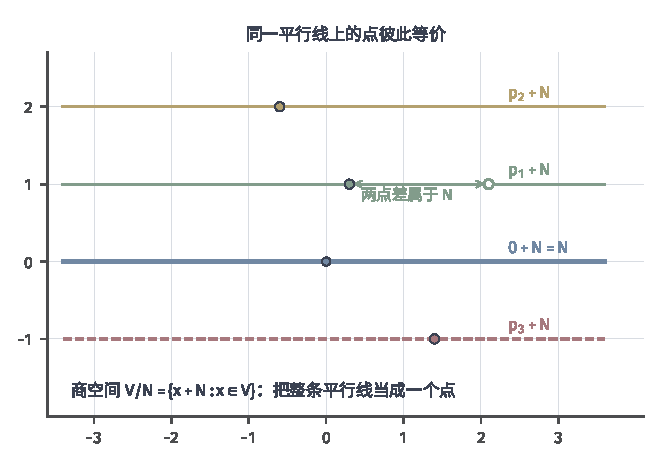
\includegraphics[width=112mm]{figures/00-shared/mathematical-preliminaries-upper/02-linear-spaces/matplotlib/ls-quotient-equivalence-classes/ls-quotient-equivalence-classes.pdf}
  \caption{商空间的等价类。$V=\mathbb R^2$，子空间$U$为$x$轴（蓝线$0+U$）；每条平行直线$p+U=\{(x,p_y)\}$是一个等价类，图中画出$y=1$（绿）、$y=2$（黄）、$y=-1$（红虚线）。绿线上实点$(0.3,1)$与空心点$(2.1,1)$之差$(1.8,0)\in U$，故属同一类；商空间$V/U$把每条平行线当成一个点。}
  \label{fig:ls-quotient-equivalence-classes}
\end{figure}

这些类能否像向量一样相加和缩放？自然的做法是借代表元来算。
\begin{definition}[商空间]
\label{def:linear-algebra-quotient-space}
设$U$是线性空间$V$的子空间。全部等价类$\bm x+U$组成的集合记为$V/U$，规定
\[
 \begin{gathered}
(\bm x+U)+(\bm y+U)=(\bm x+\bm y)+U\\
a(\bm x+U)=a\bm x+U,
 \end{gathered}
\]
称$V/U$为$V$对$U$的\term{商空间}（quotient space）。
\end{definition}
借代表元定义运算，必须先检查结果与代表元的选取无关。换代表元$\bm x'=\bm x+\bm n_1$、$\bm y'=\bm y+\bm n_2$（$\bm n_1,\bm n_2\in U$）时，$\bm x'+\bm y'$与$\bm x+\bm y$只相差$\bm n_1+\bm n_2$，$a\bm x'$与$a\bm x$只相差$a\bm n_1$，二者都属于$U$，所以得到同一个类。

零类是$U$本身，$\bm x+U$的相反类是$-\bm x+U$，其余规则由$V$的运算规则逐条继承，所以$V/U$构成线性空间。在图~\ref{fig:ls-quotient-equivalence-classes}中，两条水平线相加就是把高度相加：商空间只记录高度，被忽略的是沿$x$轴的位置。

回到截距的例子，商空间恰好只保留截距。
\begin{example}[只保留截距的商空间]
\label{ex:ls-quotient-intercept}
给定：$V=P_1=\{a+bt:a,b\in\mathbb R\}$与子空间$U=\{st:s\in\mathbb R\}$。

计算：$f_{a,b}=a+bt$所在的类是
\[
 f_{a,b}+U=\{a+(b+s)t:s\in\mathbb R\}=\{a+rt:r\in\mathbb R\},
\]
它只依赖$a$。两个类$f_{a,b}+U$与$f_{a',b'}+U$相等，当且仅当$f_{a,b}-f_{a',b'}=(a-a')+(b-b')t\in U$，即$a=a'$。按商空间的运算，
\[
 \begin{gathered}
(f_{a,b}+U)+(f_{a',b'}+U)=f_{a+a',\,b+b'}+U\\
c(f_{a,b}+U)=f_{ca,\,cb}+U,
 \end{gathered}
\]
即截距分别相加、缩放。

结论：规则$f_{a,b}+U\mapsto a$是从$P_1/U$到$\mathbb R$的双射，并保持加法与数乘。商空间$P_1/U$只记录截距，被忽略的是斜率。
\end{example}
商空间有多少个独立方向，要等下一节有了维数才能回答（第~\ref{sec:ls-dimension}节）；它与线性映射的联系在第~\ref{sec:ls-kernel-image}节给出。

% 第5章第2节：基、维数与坐标（线性无关与张成、基、维数、坐标与坐标变换）。

\section{基、维数与坐标}
\label{sec:ls-bases-dimension-coordinates}

上一节规定了在什么范围里作线性组合，但还没有回答怎样用有限个数记录一个对象。思路是选定一组方向，把对象写成它们的线性组合，用组合系数代替对象。

这要求依次回答几个问题：一组方向能到达哪些对象；到达同一个对象的系数是否唯一；怎样挑出一组既够用又不重复的方向作为“尺子”；不同的尺子是否总含同样多根，即空间有多大；选定尺子以后，系数怎样代替对象参与计算，换一把尺子系数怎样换算。前一个问题的答案是后一个问题的前提，所以按这个顺序展开。

\subsection{张成与线性无关}

\paragraph{张成}
\phantomsection
\label{sec:ls-span}
在平面上，两个不共线方向的加权组合能取到每一个点；只有一个方向时，无论怎样加权，结果都停在过原点的一条直线上。要描述一组方向“能到达哪里”，先给它们的全部线性组合命名：给定$\bm v_1,\ldots,\bm v_k\in V$，集合
\begin{equation}
 \operatorname{span}\{\bm v_1,\ldots,\bm v_k\}
 =\left\{\sum_{j=1}^k a_j\bm v_j:a_j\in\mathbb R\right\}
 \label{eq:ls-span}
\end{equation}
称为这组向量的\term{张成空间}（span）。

两个线性组合再作线性组合，仍是这组向量的线性组合，所以张成空间对线性组合封闭，是$V$的子空间。

任何包含$\bm v_1,\ldots,\bm v_k$的子空间都必须含有它们的全部线性组合，所以张成空间是包含这组向量的最小子空间。若$\operatorname{span}\{\bm v_1,\ldots,\bm v_k\}=V$，就说这组向量张成$V$，也称它们是$V$的一个生成组。

在$\mathbb R^m$中，把$\bm v_1,\ldots,\bm v_k$排成矩阵$\bm V$的各列，按列读法$\sum_ja_j\bm v_j=\bm V\bm a$，所以张成空间就是$\bm V$乘上全部系数向量所得的输出集合$\{\bm V\bm a:\bm a\in\mathbb R^k\}$，第~\ref{sec:ls-kernel-image}节将把它称为$\bm V$的列空间。如图~\ref{fig:ls-linear-combination-span}所示，两个不共线方向的组合取遍整个平面，单个方向的组合只是一条直线。
\begin{figure*}[htbp]
  \centering
  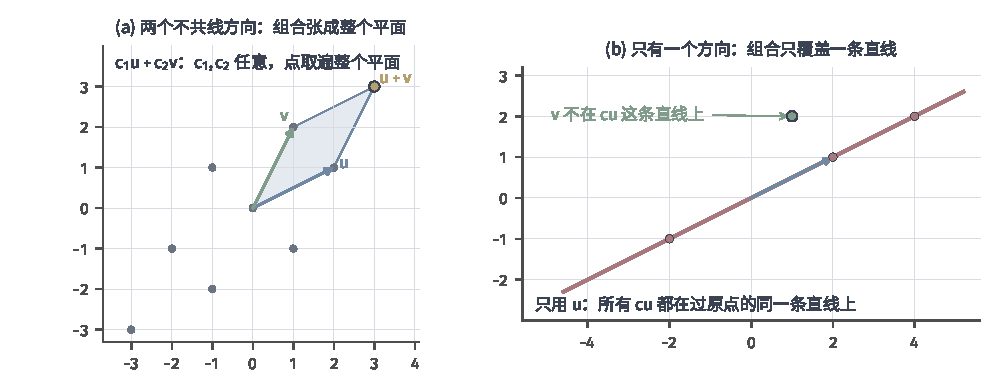
\includegraphics[width=169mm]{figures/00-shared/mathematical-preliminaries-upper/02-linear-spaces/matplotlib/ls-linear-combination-span/ls-linear-combination-span.pdf}
  \caption{两个方向与一个方向的张成范围。左：$\bm u=(2,1)$（蓝箭头）与$\bm v=(1,2)$（绿箭头）的全部加权组合取遍整个平面，浅蓝平行四边形标出$0,\bm u,\bm u+\bm v,\bm v$，灰点为整数系数格点，黄点为$\bm u+\bm v=(3,3)$。右：只有$\bm u$一个方向时，组合$\{c\bm u\}$只是过原点的一条直线（红线），$\bm v$不在其上。两图坐标等比例，为解析教学例。}
  \label{fig:ls-linear-combination-span}
\end{figure*}

\paragraph{线性无关}
\phantomsection
\label{sec:ls-linear-dependence}
张成告诉我们哪些对象能被表示，却没有说明表示方式是否只有一种。若同一个对象可以用两组不同的系数写出，某些方向就是多余的。两组系数相减，就得到零向量的一个系数不全为零的表示，所以判断冗余，只需看零向量能否被非平凡地表示。若
\begin{equation}
 a_1\bm v_1+\cdots+a_k\bm v_k=\bm0
 \label{eq:linear-algebra-independence-relation}
\end{equation}
仅在全部$a_j=0$时成立，就称这组向量\term{线性无关}（linearly independent）；否则称为\term{线性相关}（linearly dependent），即存在不全为零的系数使式\eqref{eq:linear-algebra-independence-relation}成立。线性相关时挑出一个非零系数$a_j$并移项，就能把$\bm v_j$写成其余向量的线性组合，说明这个方向重复了已有方向能到达的范围。在$\mathbb R^m$中，线性无关就是齐次方程$\bm V\bm a=\bm0$只有零解；第~\ref{sec:ls-gram-orthogonality}节还将说明，它等价于Gram矩阵$\bm V^\top\bm V$正定。

贯穿例的两列几乎同向，它们是否线性无关？
\begin{example}[近共线的两列仍线性无关]
\label{ex:ls-nearly-collinear-independence}
给定：式~\eqref{eq:linear-algebra-nearly-collinear-design}中的$\bm c_1=(1,1,1)^\top$、$\bm q=(0,1,-1)^\top$与$\bm c_2=\bm c_1+\varepsilon\bm q$。

验证：先看$\bm c_1$与$\bm q$。$\alpha\bm c_1+\beta\bm q=(\alpha,\ \alpha+\beta,\ \alpha-\beta)^\top$为零时，第一坐标给出$\alpha=0$，第二坐标再给出$\beta=0$，所以$\bm c_1,\bm q$线性无关。再看两列：
\[
 a_1\bm c_1+a_2\bm c_2=(a_1+a_2)\bm c_1+a_2\varepsilon\bm q .
\]
它为零时，由$\bm c_1,\bm q$线性无关得$a_1+a_2=0$与$a_2\varepsilon=0$。

结论：$\varepsilon\neq0$时只能$a_2=0$，进而$a_1=0$，两列线性无关；$\varepsilon=0$时$\bm c_1-\bm c_2=\bm0$，两列线性相关。
\end{example}
所以“两列几乎同向”和线性无关是两回事。线性无关是精确的是非判断，只要$\varepsilon\neq0$就成立；几乎同向描述的是接近退化的程度，要由夹角或Gram矩阵衡量，第~\ref{sec:ls-inner-product-definition}节把这种情形称为近共线。

\paragraph{表示的存在与唯一}
“能表示哪些对象”和“表示是否冗余”是两个独立的问题，分别由张成与线性无关回答。下面的例子在平面上把二者分开。
\begin{example}[足够、不够与冗余的方向组]
\label{ex:ls-redundant-spanning-set}
给定：$\mathbb R^2$中的$\bm v_1=(1,0)^{\top}$、$\bm v_2=(0,1)^{\top}$与$\bm v_3=(1,1)^{\top}$。

计算：第一，$a_1\bm v_1+a_2\bm v_2=(a_1,a_2)^{\top}$，任一目标点$(x,y)^\top$都由唯一的系数$a_1=x$、$a_2=y$取到。第二，只取$\bm v_1$时，组合$a_1\bm v_1=(a_1,0)^\top$只能到达横轴，取不到$\bm v_2$。第三，取$\bm v_1,\bm v_2,\bm v_3$时，能到达的点仍是整个平面，但目标$(1,1)^\top$有两组系数：
\[
 0\bm v_1+0\bm v_2+1\bm v_3=(1,1)^\top=1\bm v_1+1\bm v_2+0\bm v_3 .
\]
两组系数相减，得到零向量的非平凡表示$\bm v_1+\bm v_2-\bm v_3=\bm0$。

结论：$(\bm v_1,\bm v_2)$足够且无冗余；$(\bm v_1)$不够；$(\bm v_1,\bm v_2,\bm v_3)$足够，但表示冗余。
\end{example}
图~\ref{fig:vol1-add-linear-redundant-directions}把第三种情形下的两种表示画到同一个平面上。
\begin{figure}[!htb]
  \centering
  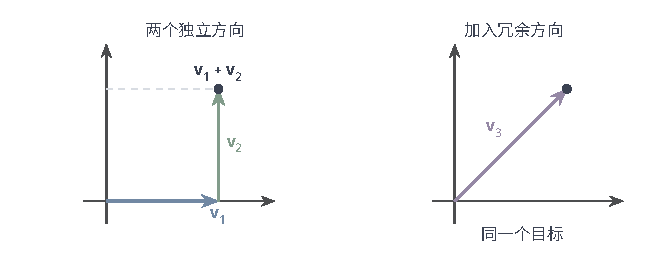
\includegraphics[width=112mm]{figures/00-shared/mathematical-preliminaries-upper/02-linear-spaces/tikz/comprehension-additions/linear-redundant-directions.pdf}
  \caption{冗余方向与重复表示。取$\bm v_1=(1,0)^{\top}$、$\bm v_2=(0,1)^{\top}$与$\bm v_3=(1,1)^{\top}$。左图沿$\bm v_1$再沿$\bm v_2$，右图直接沿$\bm v_3$，到达同一个目标；前两向量已能表示平面中的每个向量，加入$\bm v_3$只使生成组冗余。两图坐标等比例。}
  \label{fig:vol1-add-linear-redundant-directions}
\end{figure}

这个例子中的现象是一般的。存在性来自张成：张成空间之内的对象必有一组系数。唯一性来自线性无关：若同一对象有两组系数，二者相减得到式\eqref{eq:linear-algebra-independence-relation}形式的关系，无关性迫使两组系数之差为零，即两组系数完全相同。

反过来，唯一性也蕴含无关性。若存在一组不全为零的系数使线性组合为零，把这组系数加到某个对象的一组表示上，就得到同一对象的第二组表示，表示不再唯一。所以“张成空间内每个对象的系数唯一”与“零向量只有平凡表示”是同一件事的两面，这正是后面定义坐标的根据。

\subsection{基与维数}
\label{sec:ls-basis-dimension}

张成保证表示存在，无关保证表示唯一。同时满足张成和线性无关的一组向量称为\term{基}（basis）：它足够到达整个空间，又不重复，可以充当整个空间的一把“尺子”。

$\mathbb R^d$的标准坐标向量$\bm e_1,\ldots,\bm e_d$是一组基，称为标准基：$\bm x=\sum_jx_j\bm e_j$说明它们张成$\mathbb R^d$，而$\sum_ja_j\bm e_j=(a_1,\ldots,a_d)^\top=\bm0$迫使全部$a_j=0$。$P_k$中$1,t,\ldots,t^k$是一组基：每个多项式都是它们的组合，而组合为零多项式时各项系数都为零。

子空间也有基。下面为一个齐次方程的解集合求出一组基。
\begin{example}[齐次方程解平面的一组基]
\label{ex:ls-solution-plane-basis}
给定：$\mathbb R^3$中齐次方程$x_1+2x_2+3x_3=0$的解集合$N$；由示例~\ref{ex:ls-subspace-checks}，$N$是子空间。

计算：解满足$x_1=-2x_2-3x_3$，其中$x_2,x_3$可以任取，于是
\[
 \bm x=x_2(-2,1,0)^\top+x_3(-3,0,1)^\top .
\]
所以$\bm n_1=(-2,1,0)^\top$与$\bm n_2=(-3,0,1)^\top$张成$N$。若$a\bm n_1+b\bm n_2=(-2a-3b,\ a,\ b)^\top=\bm0$，比较第二、三个坐标得$a=b=0$，所以二者线性无关。

结论：$\bm n_1,\bm n_2$是$N$的一组基。
\end{example}

\paragraph{基的抽取与扩充}
若$V$有一个有限的生成组，就称$V$是有限维的；本章只讨论有限维空间。有限维空间总有基，而且可以从两个方向得到。

第一条路线是抽取。从任一有限生成组出发，若某个成员能写成其余向量的线性组合，删去它不会缩小张成范围。反复检查并删除，直到剩下的向量中没有一个能由其余向量表示。这时剩下的向量线性无关，又仍张成$V$，即构成一组基。

第二条路线是扩充。从任一线性无关组出发，逐次加入不在其张成空间中的向量。每加入一个新方向，张成范围严格扩大，新组仍线性无关：若新组的某个组合为零，新向量的系数必为零，否则新向量就能由原组表示，落在原张成空间中；新向量的系数为零以后，原组的无关性又使其余系数为零。下一小节的交换引理说明，有限维空间中线性无关组的长度不超过生成组的长度，所以扩充必在有限步内停止。停止时再也找不到张成空间之外的向量，留下的就是基。

两条路线互补：抽取把冗余的生成组压成基，扩充把线性无关组补成基。

\paragraph{维数}
\label{sec:ls-dimension}

基的向量个数是空间大小的自然度量。但先要回答一个问题：换一组基，个数会不会变？答案由交换引理给出。
\begin{theorem}[交换引理]
\label{thm:ls-exchange-lemma}
若$\bm u_1,\ldots,\bm u_r$线性无关，且每个$\bm u_i$都属于$\operatorname{span}\{\bm v_1,\ldots,\bm v_s\}$，则$r\leq s$；并且这$r$个$\bm u_i$可以逐个换入原生成组、换出同样多个$\bm v_j$，每次换完新组仍张成原来的空间。
\end{theorem}
\begin{proof}
从生成组$G_0=\{\bm v_1,\ldots,\bm v_s\}$开始。因为$\bm u_1\in\operatorname{span}G_0$，它可写成若干$\bm v_j$的组合；这些系数不能全为零，否则$\bm u_1=\bm0$，与$\bm u_1,\ldots,\bm u_r$线性无关矛盾。取某个系数非零的$\bm v_j$，从这个表达式中把它解出来，$\bm v_j$就可由$\bm u_1$与其余$\bm v$的组合表示。于是用$\bm u_1$换出$\bm v_j$，新组$G_1$与$G_0$张成同一个空间。

一般地，设第$i-1$步后的组$G_{i-1}$由$\bm u_1,\ldots,\bm u_{i-1}$和$s-(i-1)$个幸存的$\bm v$组成，且与$G_0$张成同一空间。于是$\bm u_i\in\operatorname{span}G_{i-1}$。若$\bm u_i$只用$\bm u_1,\ldots,\bm u_{i-1}$就能表示，它与前面$i-1$个方向重复，违反线性无关；所以表达式中至少一个幸存$\bm v$的系数非零，把它解出并换入$\bm u_i$，张成范围不变。只要还有幸存的$\bm v$，这一步就能做下去。

若$r>s$，换满$s$次以后组内只剩$\bm u_1,\ldots,\bm u_s$，却仍有$\bm u_{s+1}$待入列；它属于$\operatorname{span}G_s=\operatorname{span}\{\bm u_1,\ldots,\bm u_s\}$，与$r$个$\bm u$线性无关矛盾。故$r\leq s$，而上面的逐次交换正是定理要求的换入换出过程。
\end{proof}

由此，基的个数与选取无关。任取两组基，设个数分别为$r$与$s$：把第一组看成无关组、第二组看成生成组，得$r\leq s$；互换两组的角色又得$s\leq r$，所以$r=s$。这个共同的个数称为空间的\term{维数}（dimension），记为$\dim V$。只含零向量的空间以空集为基，维数为$0$。

由上一小节的例子，$\dim\mathbb R^d=d$，$\dim P_k=k+1$；方程$x_1+2x_2+3x_3=0$的解集合维数为$2$（示例~\ref{ex:ls-solution-plane-basis}），过原点的直线$\{c\bm u:c\in\mathbb R\}$（$\bm u\neq\bm0$）维数为$1$。上一节“直线”“平面”的说法现在有了确切含义。交换引理的论证依赖有限的生成组，后面的基扩充与维数计算都在这一有限维范围内进行，不能直接搬到无限维的函数展开上。

\subsection{子空间的维数与分解}
有了维数，子空间之间可以比较大小。若$U\subseteq W$，取$U$的一组基，它在$W$中仍线性无关，可以按上一小节的扩充补成$W$的基。扩充只增加向量、不删去向量，因此$\dim U\leq\dim W$；新增方向的个数恰为$\dim W-\dim U$，记录$U$之外还有多少自由度。

包含且同维时，结论收紧为相等：$\dim U=\dim W$时，把$U$的基扩充成$W$的基不需要新增任何方向，它本身已经张成$W$，故$U=W$。这里的包含条件不能省略，同维本身推不出包含。
\begin{example}[反例：同维而互不包含的两条直线]
\label{ex:ls-equal-dimension-not-nested}
给定：$\mathbb R^2$中的$U=\{(s,0)^\top:s\in\mathbb R\}$与$W=\{(s,s)^\top:s\in\mathbb R\}$。

验证：$U$以$\bm e_1$为基，$W$以$(1,1)^\top$为基，所以$\dim U=\dim W=1$。但$\bm e_1\in U$的两个坐标不相等，不在$W$中；$(1,1)^\top\in W$的第二坐标不为零，也不在$U$中。

结论：两条直线维数相同，却互不包含。维数只数方向的个数，不管这些方向具体指向哪里。
\end{example}
后面的维数公式与秩零度定理，都复用这一“先取已有基、再补新方向”的做法。

\paragraph{和的维数公式}
和空间的维数不是两边维数的简单相加，因为公共方向会被重复计入。

设$\bm z_1,\ldots,\bm z_k$是$U\cap W$的一组基，把它扩充为$U$的基$\bm z_1,\ldots,\bm z_k,\bm u_1,\ldots,\bm u_p$，再另行扩充为$W$的基$\bm z_1,\ldots,\bm z_k,\bm w_1,\ldots,\bm w_q$。下面说明这$k+p+q$个向量构成$U+W$的基。

它们张成$U+W$，因为每个$\bm u+\bm w$（$\bm u\in U$，$\bm w\in W$）都是两组基的组合。为证线性无关，设
\[
 \sum_i\alpha_i\bm z_i+\sum_j\beta_j\bm u_j+\sum_l\gamma_l\bm w_l=\bm0 .
\]
移项得$\sum_l\gamma_l\bm w_l=-\sum_i\alpha_i\bm z_i-\sum_j\beta_j\bm u_j$。左边属于$W$，右边属于$U$，所以这个向量属于$U\cap W$，可以写成$\sum_i\delta_i\bm z_i$。于是$\sum_l\gamma_l\bm w_l-\sum_i\delta_i\bm z_i=\bm0$，由$W$的基线性无关，全部$\gamma_l=0$。代回原式，再由$U$的基线性无关，全部$\alpha_i$与$\beta_j$也为零。因此$\dim(U+W)=k+p+q=(k+p)+(k+q)-k$，即
\begin{equation}
 \dim(U+W)=\dim U+\dim W-\dim(U\cap W).
 \label{eq:ls-dimension-formula}
\end{equation}
被减去的维数正是两边重复计入的公共方向，而不是两个集合元素个数的差。下面在$\mathbb R^3$中核对这一公式。
\begin{example}[两个坐标平面的和]
\label{ex:ls-dimension-formula-planes}
给定：$\mathbb R^3$中的$U=\operatorname{span}\{\bm e_1,\bm e_2\}$与$W=\operatorname{span}\{\bm e_2,\bm e_3\}$。

计算：$U$由第三坐标为零的向量组成，$W$由第一坐标为零的向量组成，所以$U\cap W$由第一、三坐标都为零的向量组成，即$U\cap W=\operatorname{span}\{\bm e_2\}$，维数为$1$。$U+W$含有$\bm e_1,\bm e_2,\bm e_3$，所以$U+W=\mathbb R^3$。代入公式：
\[
 \dim(U+W)=3=2+2-1 .
\]
若改取两条坐标轴$U'=\operatorname{span}\{\bm e_1\}$、$W'=\operatorname{span}\{\bm e_2\}$，交为零，$\dim(U'+W')=1+1-0=2$。

结论：公式中减去的$1$正是两个平面共有的$\bm e_2$方向；交为零时，和的维数等于两边维数之和。
\end{example}

\paragraph{补空间的存在}
第~\ref{sec:ls-direct-sum}节定义了补空间，现在可以说明它总存在。把$U$的基扩充为$V$的基，新增向量张成的子空间记为$W$。整组基张成$V$，所以$U+W=V$。若某向量同属$U$与$W$，它既是$U$的基向量的组合，又是新增向量的组合，两种写法相减，得到整组基的一个组合为零，系数只能全为零，所以$U\cap W=\{\bm0\}$。于是$V=U\oplus W$。由维数公式，直和时交的维数为零，$\dim V=\dim U+\dim W$。扩充的选择不唯一，补空间也就不唯一，这与平面中直线的例子一致。

\paragraph{商空间的维数}
同样的“先取已有基、再补新方向”也回答了第~\ref{sec:ls-quotient-spaces}节留下的问题：商空间$V/U$有多少个独立方向？取$U$的一组基$\bm u_1,\ldots,\bm u_s$并扩充为$V$的基$\bm u_1,\ldots,\bm u_s,\bm w_1,\ldots,\bm w_t$。新增向量的类$\bm w_1+U,\ldots,\bm w_t+U$张成$V/U$：任一$\bm x$写成整组基的组合，其中$U$部分落进零类被消去。

这些类也线性无关：若$\sum_ja_j(\bm w_j+U)=U$，则$\sum_ja_j\bm w_j\in U$，它能由$\bm u_i$表示，整组基的线性无关性迫使全部$a_j=0$。因此
\begin{equation}
 \dim(V/U)=\dim V-\dim U.
 \label{eq:ls-quotient-dimension}
\end{equation}

商空间的维数恰好等于补空间的维数。新增方向$\bm w_j$张成$U$的一个补空间$W$，每个$\bm x$唯一分解为$\bm x=\bm u+\bm w$（$\bm u\in U$，$\bm w\in W$），于是类$\bm x+U=\bm w+U$中的点都形如$\bm w+\bm u'$（$\bm u'\in U$）。这样的点落在$W$中当且仅当$\bm u'\in U\cap W=\{\bm0\}$，所以每个类与$W$恰交于一点$\bm w$。选定补空间，就是为每个类选定一个代表元。补空间要选，商空间却不依赖任何选择，这是二者的区别。

示例~\ref{ex:ls-quotient-intercept}中，$\dim(P_1/U)=2-1=1$，商空间只剩截距这一个方向；图~\ref{fig:ls-quotient-equivalence-classes}中，$\dim(\mathbb R^2/U)=1$，只剩高度。

\subsection{坐标与坐标变换}
\label{sec:ls-coordinates}
\label{sec:linear-algebra-coordinates}

有了基，每个对象都有唯一的一组系数。怎样用这组系数代替对象参与计算？代替以后，系数的大小能否反映对象的大小？换一组基，系数怎样换算？本小节依次回答这三个问题。

\paragraph{有序基下的坐标}
固定有序基$\mathcal B=(\bm b_1,\ldots,\bm b_d)$后，对象$\bm v$唯一写成$\sum_{j=1}^d x_j\bm b_j$。系数列$[\bm v]_{\mathcal B}=(x_1,\ldots,x_d)^{\top}$称为$\bm v$在基$\mathcal B$下的\term{坐标}（coordinates）。

存在性来自张成，唯一性来自线性无关，所以坐标映射$\bm v\mapsto[\bm v]_{\mathcal B}$是从$V$到$\mathbb R^d$的双射：每个对象恰有一列坐标，每列实数$(x_1,\ldots,x_d)^{\top}$也恰好记录对象$\sum_jx_j\bm b_j$。

它还保持线性组合：若$[\bm v]_{\mathcal B}=\bm x$、$[\bm w]_{\mathcal B}=\bm y$，则$a\bm v+b\bm w=\sum_j(ax_j+by_j)\bm b_j$，由唯一性得$[a\bm v+b\bm w]_{\mathcal B}=a\bm x+b\bm y$。因此对象上的线性运算可以完全交给坐标去算，算完再按基还原。

在$\mathbb R^d$中，把基向量排成矩阵$\bm B=[\bm b_1\ \cdots\ \bm b_d]$，按列读法$\bm v=\bm B[\bm v]_{\mathcal B}$，所以坐标就是方程$\bm B\bm x=\bm v$的唯一解。下面用这一方程求一个斜基下的坐标。
\begin{example}[同一向量在两组基下的坐标]
\label{ex:ls-coordinates-two-bases}
给定：$\mathbb R^2$中的向量$\bm x=(1,2)^\top$，标准基$(\bm e_1,\bm e_2)$，以及斜基$\mathcal B=(\bm b_1,\bm b_2)$，$\bm b_1=(2,1)^\top$、$\bm b_2=(-1,1)^\top$。

计算：标准基下$\bm x=1\cdot\bm e_1+2\cdot\bm e_2$，坐标为$(1,2)^\top$。斜基下的坐标$(c_1,c_2)^\top$满足$c_1\bm b_1+c_2\bm b_2=\bm x$，即
\[
 \begin{gathered}
2c_1-c_2=1\\
c_1+c_2=2 .
 \end{gathered}
\]
两式相加得$3c_1=3$，所以$c_1=1$、$c_2=1$。核对：$\bm b_1+\bm b_2=(1,2)^\top$。

结论：$[\bm x]_{\mathcal B}=(1,1)^\top$。向量本身没有移动，只是沿不同的基去量。
\end{example}
图~\ref{fig:ls-basis-coordinates}画出这两种读法。
\begin{figure*}[htbp]
  \centering
  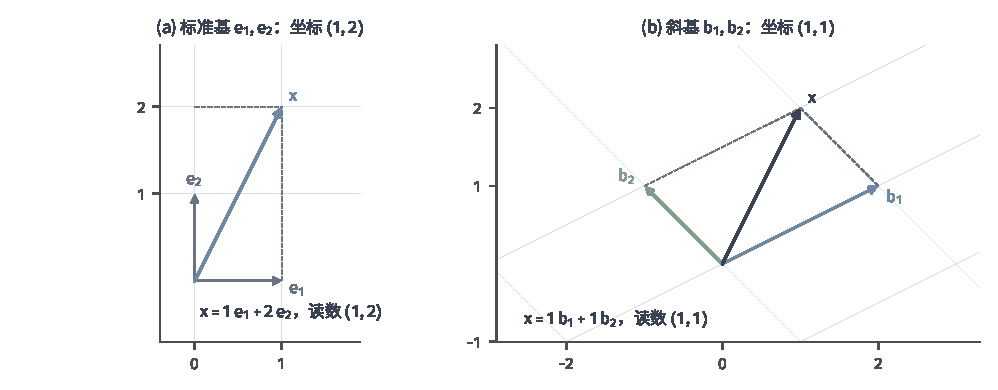
\includegraphics[width=169mm]{figures/00-shared/mathematical-preliminaries-upper/02-linear-spaces/matplotlib/ls-basis-coordinates/ls-basis-coordinates.pdf}
  \caption{同一向量在两组基下的坐标。左：标准基$\bm e_1,\bm e_2$（灰箭头）下，向量$\bm x=(1,2)$（蓝箭头）的坐标为$(1,2)$，虚线为向坐标轴的垂线。右：斜基$\bm b_1=(2,1)$（蓝）、$\bm b_2=(-1,1)$（绿）下，同一个$\bm x$满足$\bm x=\bm b_1+\bm b_2$，坐标为$(1,1)$，浅色斜线为斜基网格，虚线为平行四边形读法。两图坐标系相同。}
  \label{fig:ls-basis-coordinates}
\end{figure*}

\paragraph{坐标与对象}
坐标列要与它所记录的对象区分开：几何位移、有限信号、多项式都可以相加和缩放，它们是\emph{对象}；一列实数只是选定基以后记录对象的\emph{坐标}。基的顺序也要固定：交换$\bm b_1,\bm b_2$，对象不变，坐标列的前两个数也随之交换。在$\mathbb R^d$中直接写数字列，通常是默认使用标准基$\bm e_1,\ldots,\bm e_d$，这时对象与坐标恰好是同一列数，第~\ref{chap:linear-operations}章正是在这种默认下工作的。

函数的基展开则必须区分二者：函数是对象，展开系数是坐标。
\begin{example}[仿射函数在两组基下的坐标]
\label{ex:ls-affine-function-coordinates}
给定：$P_1$中的$f_{a,b}=a+bt$，以及两组基$\mathcal B_1=(1,t)$与$\mathcal B_2=(1,1+t)$。

计算：在$\mathcal B_1$下$f_{a,b}=a\cdot1+b\cdot t$，坐标为$(a,b)^\top$。在$\mathcal B_2$下设$f_{a,b}=c_1\cdot1+c_2(1+t)=(c_1+c_2)+c_2t$，比较常数项与$t$的系数，得$c_2=b$、$c_1=a-b$，即
\[
 f_{a,b}=(a-b)\cdot1+b\cdot(1+t).
\]

结论：同一个函数在$\mathcal B_1$与$\mathcal B_2$下的坐标分别是$(a,b)^\top$与$(a-b,b)^\top$；坐标改变了，函数本身没有改变。
\end{example}
坐标的个数总是维数。一个对象若用冗余的生成组记录，记录的长度可以超过维数，所以不能由这种记录的长度推断空间有几维。

\paragraph{坐标对基的敏感性}
对象不变时，坐标仍可能相差很大。贯穿例给出一个数值上很极端的情形。
\begin{example}[近共线基下的大坐标]
\label{ex:ls-coordinate-instability}
给定：示例~\ref{ex:ls-nearly-collinear-independence}中的$\bm c_1,\bm q$与$\bm c_2=\bm c_1+\varepsilon\bm q$（$\varepsilon\neq0$），$\delta=0.1$，以及目标向量
\begin{equation}
 \bm y=\bm c_1+\delta\bm q=\begin{bmatrix}1\\1.1\\0.9\end{bmatrix}.
 \label{eq:linear-algebra-nearly-collinear-target}
\end{equation}
由该示例，$\mathcal B_0=(\bm c_1,\bm q)$与$\mathcal B_\varepsilon=(\bm c_1,\bm c_2)$都是平面$\operatorname{span}\{\bm c_1,\bm q\}$的基，$\bm y$也在这个平面中。

计算：在$\mathcal B_0$下，$\bm y$的坐标是$(1,\delta)^{\top}$。在$\mathcal B_\varepsilon$下，把$\bm q=(\bm c_2-\bm c_1)/\varepsilon$代入$\bm y=\bm c_1+\delta\bm q$，得
\begin{equation}
 \bm y=\left(1-\frac{\delta}{\varepsilon}\right)\bm c_1
       +\frac{\delta}{\varepsilon}\bm c_2.
 \label{eq:linear-algebra-coordinate-instability}
\end{equation}
取$\varepsilon=0.01$，则$\delta/\varepsilon=10$，坐标成为$(-9,10)^{\top}$。

结论：同一个$\bm y$在$\mathcal B_0$下的坐标为$(1,0.1)^\top$，在$\mathcal B_{0.01}$下的坐标为$(-9,10)^\top$。
\end{example}
两个很大的系数在几乎同向的两个基向量上相互抵消，不能据此判断原对象很大。这种系数对接近退化的基的敏感，将在第~\ref{chap:linear-analysis}章定量讨论。新旧坐标之间怎样系统地换算，是下面要回答的问题。

\paragraph{换基矩阵}
\phantomsection
\label{sec:ls-change-basis}
\label{sec:linear-algebra-coordinate-conversions}
设$\mathcal B=(\bm b_1,\ldots,\bm b_d)$与$\mathcal C$是$V$的两组有序基。已知$\bm v$在$\mathcal B$下的坐标$[\bm v]_{\mathcal B}=(x_1,\ldots,x_d)^{\top}$，怎样求它在$\mathcal C$下的坐标？由$\bm v=\sum_jx_j\bm b_j$，并且坐标映射保持线性组合，
\[
 [\bm v]_{\mathcal C}=\sum_{j=1}^d x_j[\bm b_j]_{\mathcal C}.
\]
右边是各列$[\bm b_j]_{\mathcal C}$以$x_j$为权重的线性组合。把这些列排成矩阵，称为从$\mathcal B$到$\mathcal C$的换基矩阵$\bm S_{\mathcal C\leftarrow\mathcal B}$，按矩阵与向量乘积的列读法，
\begin{equation}
 [\bm v]_{\mathcal C}
 =\bm S_{\mathcal C\leftarrow\mathcal B}[\bm v]_{\mathcal B}.
 \label{eq:linear-algebra-coordinate-change}
\end{equation}
换基矩阵的第$j$列是旧基向量$\bm b_j$的新坐标；下标$\mathcal C\leftarrow\mathcal B$从右向左读，表示把$\mathcal B$坐标译成$\mathcal C$坐标。下面在平面上算一个具体的换基矩阵。
\begin{example}[平面上的换基矩阵]
\label{ex:ls-change-of-basis-plane}
给定：$\mathbb R^2$的标准基$\mathcal E$与基$\mathcal U=(\bm u_1,\bm u_2)$，$\bm u_1=(1,0)^{\top}$、$\bm u_2=(1,1)^{\top}$；向量$\bm v$在$\mathcal U$下的坐标为$(1,1)^\top$。

计算：$\bm u_1,\bm u_2$的标准坐标就是它们自己。按“第$j$列是旧基向量的新坐标”，
\[
 \bm S_{\mathcal E\leftarrow\mathcal U}=\begin{bmatrix}1&1\\0&1\end{bmatrix}.
\]
由式~\eqref{eq:linear-algebra-coordinate-change}，$[\bm v]_{\mathcal E}=\bm S_{\mathcal E\leftarrow\mathcal U}(1,1)^{\top}=(2,1)^{\top}$。直接核对：$\bm v=\bm u_1+\bm u_2=(2,1)^\top$。

结论：$\mathcal U$坐标$(1,1)^\top$与标准坐标$(2,1)^\top$记录的是同一个向量。
\end{example}
图~\ref{fig:vol1-add-linear-change-basis}画出这一点：目标位置没有移动，改变的只是沿哪两条基方向累加，以及每条方向取多少份。
\begin{figure}[!htb]
  \centering
  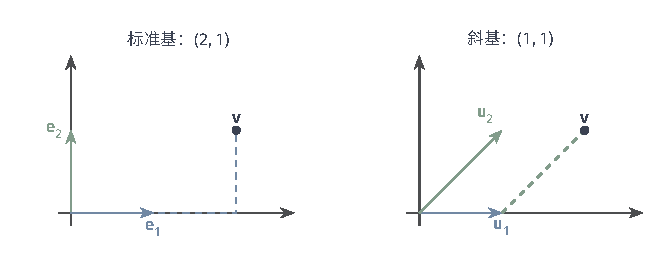
\includegraphics[width=112mm]{figures/00-shared/mathematical-preliminaries-upper/02-linear-spaces/tikz/comprehension-additions/linear-change-basis.pdf}
  \caption{同一向量的两套坐标。左图使用标准基，$\bm v=(2,1)^{\top}$的坐标为$(2,1)^{\top}$；右图使用$\bm u_1=(1,0)^{\top}$、$\bm u_2=(1,1)^{\top}$，同一$\bm v$的坐标为$(1,1)^{\top}$。虚线表示相应的向量相加，两图的环境坐标比例相同。}
  \label{fig:vol1-add-linear-change-basis}
\end{figure}

\paragraph{连续换基与反向换基}
若再换到第三组基$\mathcal D$，中间那套坐标应当不留痕迹。对每个$\bm v$，连用两次式~\eqref{eq:linear-algebra-coordinate-change}，
\[
 [\bm v]_{\mathcal D}=\bm S_{\mathcal D\leftarrow\mathcal C}[\bm v]_{\mathcal C}=\bm S_{\mathcal D\leftarrow\mathcal C}\bm S_{\mathcal C\leftarrow\mathcal B}[\bm v]_{\mathcal B}.
\]
取$\bm v=\bm b_j$，它的$\mathcal B$坐标是$\bm e_j$，两边读出的分别是$\bm S_{\mathcal D\leftarrow\mathcal B}$与乘积的第$j$列，所以
\[
 \bm S_{\mathcal D\leftarrow\mathcal B}
 =\bm S_{\mathcal D\leftarrow\mathcal C}\bm S_{\mathcal C\leftarrow\mathcal B}.
\]

特别取$\mathcal D=\mathcal B$。每个$\bm b_j$在$\mathcal B$下的坐标是$\bm e_j$，所以左边$\bm S_{\mathcal B\leftarrow\mathcal B}=\bm I_d$，即$\bm S_{\mathcal B\leftarrow\mathcal C}\bm S_{\mathcal C\leftarrow\mathcal B}=\bm I_d$；交换两组基的角色，同理得$\bm S_{\mathcal C\leftarrow\mathcal B}\bm S_{\mathcal B\leftarrow\mathcal C}=\bm I_d$。所以换基矩阵总可逆，反向换基矩阵就是它的逆：$\bm S_{\mathcal B\leftarrow\mathcal C}=\bm S_{\mathcal C\leftarrow\mathcal B}^{-1}$。在示例~\ref{ex:ls-change-of-basis-plane}中，$\bm S_{\mathcal U\leftarrow\mathcal E}=\bm S_{\mathcal E\leftarrow\mathcal U}^{-1}=\left[\begin{smallmatrix}1&-1\\0&1\end{smallmatrix}\right]$，它把$(2,1)^{\top}$送回$(1,1)^{\top}$。

反过来，任一$d$阶可逆矩阵$\bm P$都是某次换基的矩阵。以$\bm P$的第$j$列为$\mathcal B$坐标，取向量$\bm b'_j=\sum_i\bm P_{i,j}\bm b_i$。$\bm P$的列线性无关，而坐标映射是保持线性组合的双射，所以$\bm b'_1,\ldots,\bm b'_d$也线性无关。个数等于维数的线性无关组必是基：否则它还能扩充，得到多于$\dim V$个线性无关的向量，与交换引理矛盾。于是$\bm b'_1,\ldots,\bm b'_d$构成一组基$\mathcal B'$。按定义，$\bm S_{\mathcal B\leftarrow\mathcal B'}$的第$j$列是$\bm b'_j$的$\mathcal B$坐标，即$\bm P$的第$j$列，所以$\bm S_{\mathcal B\leftarrow\mathcal B'}=\bm P$。

反向换基的代价取决于换基矩阵是否接近不可逆。贯穿例把这一点表现得很清楚。
\begin{example}[近共线基之间的换基]
\label{ex:ls-nearly-collinear-change-of-basis}
给定：示例~\ref{ex:ls-coordinate-instability}中的两组基$\mathcal B_0=(\bm c_1,\bm q)$与$\mathcal B_\varepsilon=(\bm c_1,\bm c_2)$，$\varepsilon\neq0$。

计算：由$\bm c_1=1\cdot\bm c_1+0\cdot\bm q$与$\bm c_2=1\cdot\bm c_1+\varepsilon\bm q$，$\mathcal B_\varepsilon$的两个向量在$\mathcal B_0$下的坐标分别是$(1,0)^{\top}$与$(1,\varepsilon)^{\top}$，所以
\[
\begin{gathered}
\bm S_{\mathcal B_0\leftarrow\mathcal B_\varepsilon}
 =\begin{bmatrix}1&1\\0&\varepsilon\end{bmatrix}\\
\bm S_{\mathcal B_\varepsilon\leftarrow\mathcal B_0}
 =\bm S_{\mathcal B_0\leftarrow\mathcal B_\varepsilon}^{-1}
 =\begin{bmatrix}1&-1/\varepsilon\\0&1/\varepsilon\end{bmatrix},
\end{gathered}
\]
后者可由直接相乘验证。把$\bm y$在$\mathcal B_0$下的坐标$(1,\delta)^{\top}$代入后者，得
\[
 \bm S_{\mathcal B_\varepsilon\leftarrow\mathcal B_0}\begin{bmatrix}1\\\delta\end{bmatrix}
 =\begin{bmatrix}1-\delta/\varepsilon\\\delta/\varepsilon\end{bmatrix},
\]
与式~\eqref{eq:linear-algebra-coordinate-instability}一致。

结论：$\bm S_{\mathcal B_0\leftarrow\mathcal B_\varepsilon}$的行列式为$\varepsilon$，接近零；反向换基矩阵含有因子$1/\varepsilon$，小的基差异由此被放大成大系数。
\end{example}

\paragraph{被动换基与主动作用}
被动换基与主动作用必须分开。换基时对象不动、记录改变，式\eqref{eq:linear-algebra-coordinate-change}两侧是同一个$\bm v$的两套坐标；主动作用则在固定的坐标下把对象送到另一个对象，例如第~\ref{chap:linear-operations}章的矩阵作用$\bm x\mapsto\bm A\bm x$把向量旋转或切变，下一节把它推广为线性映射。

两者都写成矩阵乘以坐标列，形式相似，含义不同。下面的例子在同一个初始向量上比较两种情形。
\begin{example}[被动换基与主动切变]
\label{ex:ls-passive-vs-active}
给定：$\mathbb R^2$中的向量$\bm x=(3,3)^\top$，斜基$\mathcal B'=(\bm b_1,\bm b_2)$，$\bm b_1=(2,1)^\top$、$\bm b_2=(-1,1)^\top$，以及切变矩阵$\bm A=\left[\begin{smallmatrix}1&1\\0&1\end{smallmatrix}\right]$。

计算：被动换基时，求$\bm x$在$\mathcal B'$下的坐标$(c_1,c_2)^\top$。由$2c_1-c_2=3$与$c_1+c_2=3$得$c_1=2$、$c_2=1$，即$\bm x=2\bm b_1+\bm b_2$。主动作用时，计算$\bm A\bm x=(3+3,\ 3)^\top=(6,3)^\top$。

结论：前者中向量仍是$(3,3)^\top$，只是读数从$(3,3)$变成$(2,1)$；后者中坐标系不动，向量本身被搬到$(6,3)^\top$。
\end{example}
图~\ref{fig:ls-passive-change-vs-active-map}把两种情形并排画出。所以不能把所有乘矩阵的运算都理解成换基。
\begin{figure*}[htbp]
  \centering
  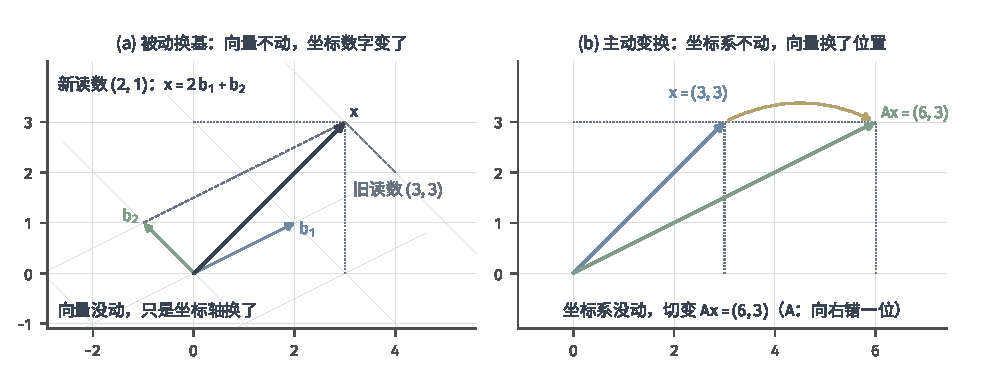
\includegraphics[width=169mm]{figures/00-shared/mathematical-preliminaries-upper/02-linear-spaces/matplotlib/ls-passive-change-vs-active-map/ls-passive-change-vs-active-map.pdf}
  \caption{被动换基与主动变换的对照，两图使用同一个初始向量$\bm x=(3,3)$。左（被动换基）：箭头位置不动（深色），旧标准读数用点线投影读出$(3,3)$；新斜基$\bm b_1=(2,1)$（蓝）、$\bm b_2=(-1,1)$（绿）与浅色斜网格下，$\bm x=2\bm b_1+\bm b_2$，新读数为$(2,1)$。右（主动变换）：标准坐标系不动，$\bm x$（蓝）被切变映到$\bm A\bm x=(6,3)$（绿），黄色弧线表示搬动过程。}
  \label{fig:ls-passive-change-vs-active-map}
\end{figure*}

% 第5章第3节：线性映射（定义；表示：矩阵表示、基于矩阵的映射运算、矩阵基本子空间；核与像、秩零度、商空间、行空间与列空间、可逆性；换基：相抵与相似）。

\section{线性与多线性映射}
\label{sec:ls-linear-maps}
\label{sec:linear-algebra-matrices-linear-maps}

前两节研究的是单个空间中的对象怎样记录；本节转向对象之间的作用。一个作用要满足什么条件，才能用前两节的语言处理？选定基以后，它怎样记录成一张数表，两个作用叠加或接连进行时数表怎样变化？作用保留了哪些输入信息、丢失了哪些，什么时候可以由输出唯一反求输入？换一组基，记录同一个作用的数表怎样改变，哪些量不随之改变？本节的四个小节依次回答这四个问题。

\subsection{线性映射及其矩阵表示}
\label{sec:ls-linear-map-definition}
\label{sec:linear-algebra-maps}

设计矩阵把一组系数变成一列拟合值，求导把一个多项式变成另一个多项式，读取第一个坐标把向量变成一个数。这些作用有一个共同点：输入先加权相加再作用，与先分别作用再作同样的加权相加，结果相同。正是这一点让前两节的语言可以用于作用本身：输入写成基向量的组合，作用就可以逐个基向量地计算。保持线性组合的作用称为\term{线性映射}（linear map）$T:V\to W$：
\begin{equation}
\begin{gathered}
T(a\bm x+b\bm y)=aT\bm x+bT\bm y\\
\bm x,\bm y\in V,\ a,b\in\mathbb R.
\end{gathered}
\label{eq:ls-linear-map-def}
\end{equation}
取$a=b=0$得$T\bm0=\bm0$，线性映射总把原点留在原处。由式~\eqref{eq:prelim-matrix-linearity}，任何矩阵$\bm A\in\mathbb R^{m\times d}$给出的$\bm x\mapsto\bm A\bm x$都是从$\mathbb R^d$到$\mathbb R^m$的线性映射。下面再检查几个作用是否线性。
\begin{example}[线性与非线性的作用]
\label{ex:ls-linear-map-checks}
给定：三个作用
\[
 \begin{aligned}
 &T:\mathbb R^2\to\mathbb R^2, &&T(x_1,x_2)=(2x_1+x_2,\ 3x_2);\\
 &D:P_k\to P_k, &&Dp=p';\\
 &\tau:\mathbb R\to\mathbb R, &&\tau(x)=x+1.
 \end{aligned}
\]

验证：$T(x_1,x_2)$就是$\left[\begin{smallmatrix}2&1\\0&3\end{smallmatrix}\right]\bm x$，所以$T$保持线性组合。对多项式有$(ap+bq)'=ap'+bq'$，所以$D$保持线性组合；求导不升高次数，$D$确实把$P_k$送回$P_k$。$\tau(0)=1\neq0$，而线性映射必把$0$送到$0$。

结论：$T$与$D$是线性映射，$\tau$不是线性映射。
\end{example}

\phantomsection
\label{sec:ls-operator-powers}
输入与输出是同一个空间的线性映射$T:V\to V$称为\term{线性算子}（linear operator），也称线性变换。平面上的旋转、向一条直线的投影、$P_k$上的求导都是线性算子，示例~\ref{ex:ls-linear-map-checks}中的$T$也是。

算子是映射的特殊情形，但这一限制带来两点实质的不同。第一，输出仍在$V$中，可以再次作为输入，所以算子能与自身复合、反复作用：记$T^2=T\circ T$、$T^k=T\circ T^{k-1}$，并约定$T^0=\operatorname{id}_V$；一般映射$V\to W$在$V\neq W$时不能这样反复作用。下面将看到，在同一组基下，$T^k$的矩阵就是$T$的矩阵的$k$次幂。

第二，记录算子时输入、输出可以用同一组基，这决定了算子换基时的特殊规律（第~\ref{sec:ls-similarity}节）。

\paragraph{坐标表示与运算}
\label{sec:ls-map-representation}

线性映射的定义域通常有无穷多个元素，逐个记录输出是不可能的。本小节说明，有了基，有限个数就够了：在固定的两组基下，线性映射与矩阵一一对应，映射的叠加、复合与求逆分别对应矩阵的加法、乘法与求逆。第~\ref{chap:linear-operations}章的矩阵运算由此获得一般含义：矩阵就是线性映射在坐标下的记录。下面先建立这一对应，再把映射的运算翻译成矩阵的运算，最后对矩阵定义四个基本子空间，供下一小节计数信息的丢失与保留。

\subsubsection{矩阵表示}

给定输入基$\mathcal B=(\bm b_1,\ldots,\bm b_d)$，任一$\bm v=\sum_jx_j\bm b_j$的像由线性性写成
\[
 T\bm v=\sum_{j=1}^d x_j\,T\bm b_j,
\]
所以只要知道$d$个基向量的像，整个映射就确定了。再给定输出基$\mathcal C$，把每个像的坐标$[T\bm b_j]_{\mathcal C}$作为第$j$列，排成矩阵$\bm A=[T]_{\mathcal C\leftarrow\mathcal B}\in\mathbb R^{m\times d}$，称为$T$在这两组基下的矩阵。对上式两边取$\mathcal C$坐标，由坐标映射保持线性组合，并按矩阵与向量乘积的列读法，得到
\begin{equation}
 [T\bm v]_{\mathcal C}
 =\sum_{j=1}^d x_j\,[T\bm b_j]_{\mathcal C}
 =\sum_{j=1}^d x_j\bm A_{:,j}
 =[T]_{\mathcal C\leftarrow\mathcal B}\,[\bm v]_{\mathcal B}.
 \label{eq:linear-algebra-map-matrix-representation}
\end{equation}
也就是说，输出坐标等于矩阵乘以输入坐标：作用在对象上进行，记录在坐标上进行，二者由矩阵与向量的乘积连接。列数是输入维数，行数是输出维数；下标$\mathcal C\leftarrow\mathcal B$从右向左读，表示输入用$\mathcal B$记录、输出用$\mathcal C$记录。输入输出为同一空间的算子通常两端用同一组基，记为$[T]_{\mathcal B}=[T]_{\mathcal B\leftarrow\mathcal B}$，它是$\dim V$阶方阵。

下面按这一规则写出两个映射的矩阵。
\begin{example}[由基向量的像写出矩阵]
\label{ex:ls-plane-operator-matrix}
给定：示例~\ref{ex:ls-linear-map-checks}中的$T(x_1,x_2)=(2x_1+x_2,\ 3x_2)$，输入输出都取标准基。

计算：$T\bm e_1=(2,0)^{\top}$，$T\bm e_2=(1,3)^{\top}$。把它们依次作为两列，得
\[
 [T]=\begin{bmatrix}2&1\\0&3\end{bmatrix}.
\]

结论：$[T]$正是定义$T$时用的矩阵。
\end{example}
一般地，$\bm x\mapsto\bm A\bm x$在标准基下的矩阵就是$\bm A$本身，因为$\bm A\bm e_j=\bm A_{:,j}$。矩阵表示同样适用于不是数组的对象。
\begin{example}[求导的矩阵表示]
\label{ex:ls-derivative-matrix}
给定：求导$D:P_2\to P_2$，输入输出都取基$(1,t,t^2)$。

计算：$D1=0$，$Dt=1$，$Dt^2=2t$，三个像的坐标依次为$(0,0,0)^\top$、$(1,0,0)^\top$、$(0,2,0)^\top$，所以
\[
 [D]=\begin{bmatrix}0&1&0\\0&0&2\\0&0&0\end{bmatrix}.
\]
多项式$p=a_0+a_1t+a_2t^2$的坐标是$(a_0,a_1,a_2)^\top$，而$[D](a_0,a_1,a_2)^\top=(a_1,2a_2,0)^\top$，正是$p'=a_1+2a_2t$的坐标。

结论：对函数求导，在坐标下就是乘矩阵$[D]$。
\end{example}

\begin{theorem}[线性映射与矩阵的对应]
\label{thm:ls-map-matrix-correspondence}
设$\dim V=d$、$\dim W=m$，并固定$V$的基$\mathcal B$与$W$的基$\mathcal C$。则$T\mapsto[T]_{\mathcal C\leftarrow\mathcal B}$是从全部线性映射$V\to W$到全部$m\times d$实矩阵的双射。
\end{theorem}
\begin{proof}
单射：若两个线性映射的矩阵相同，它们在每个基向量上的像相同，由$T\bm v=\sum_jx_jT\bm b_j$，它们在每个$\bm v$上都相同。满射：任给$\bm A\in\mathbb R^{m\times d}$，对$\bm v\in V$令$T\bm v$为$\mathcal C$坐标等于$\bm A[\bm v]_{\mathcal B}$的那个向量。坐标唯一，所以这一规则有确定的意义；坐标映射与乘矩阵都保持线性组合，所以$T$线性；$T\bm b_j$的坐标是$\bm A\bm e_j=\bm A_{:,j}$，所以$[T]_{\mathcal C\leftarrow\mathcal B}=\bm A$。
\end{proof}
所以基固定以后，线性映射与矩阵一一对应；每个从$\mathbb R^d$到$\mathbb R^m$的线性映射在标准基下都等于乘某个矩阵。不过这一对应依赖基的选取：改变两端任一组基，通常会改变数表，而数表记录的仍是同一个映射。数表具体怎样随基改变，在第~\ref{sec:ls-coordinates-change-of-basis}节推导。

设计矩阵$\bm X_\varepsilon$正是这样一张记录：它表示$T_\varepsilon:\mathbb R^2\to\mathbb R^3$，$\bm w\mapsto\bm X_\varepsilon\bm w=w_1\bm c_1+w_2\bm c_2$，两列分别是两个输入基向量的像。输入是两个系数，输出是三个样本的拟合值，二者不能当成同一个空间中的向量。矩阵只是映射在两端坐标下的记录，不是映射本身的全部含义。图~\ref{fig:ch06-object-coordinate-map}中两条路径给出同一结果：先作用于对象再取坐标，与先取输入坐标再乘矩阵，得到相同的输出坐标。
\begin{figure}[htbp]
  \centering
  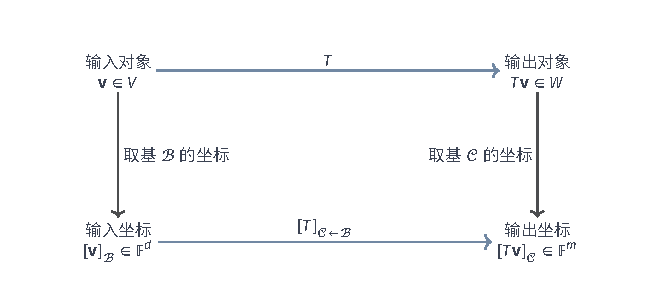
\includegraphics[width=112.0mm]{figures/00-shared/mathematical-preliminaries-upper/02-linear-spaces/tikz/ch06-object-coordinate-map/figure.pdf}
  \caption{先作用于对象再取坐标，与先取输入坐标再按矩阵的列作线性组合（即乘矩阵），得到相同输出坐标。横向箭头改变对象或数值，竖向箭头只改变记录方式。}
  \label{fig:ch06-object-coordinate-map}
\end{figure}

\subsubsection{基于矩阵的映射运算}
\phantomsection
\label{sec:ls-map-addition-composition}

两个映射可以把输出相加，也可以接连作用；一个映射可能可以撤销，也可能带上常数偏置。第~\ref{chap:linear-operations}章的矩阵加法、乘法与求逆，正是前三种运算在固定基下的记录；带偏置的仿射映射则可以借增广坐标写成一张更大的矩阵。

\paragraph{叠加}
\phantomsection
\label{sec:linear-algebra-map-addition}
设$T,S:V\to W$是同一对空间之间的两个线性映射，定义
\[
\begin{gathered}
(aT+bS)(\bm x)=aT\bm x+bS\bm x\\
\bm x\in V,
\end{gathered}
\]
其中$a,b\in\mathbb R$。叠加保持线性：把输入的线性组合代入，两个分支分别展开再汇总即可。在$V$与$W$的固定基下，若$T,S$的矩阵为$\bm A,\bm B$，则$aT+bS$把第$j$个基向量送到$aT\bm b_j+bS\bm b_j$，其坐标是$a\bm A_{:,j}+b\bm B_{:,j}$，所以$aT+bS$的矩阵就是$a\bm A+b\bm B$。

相加的前提是两个映射的定义域与陪域都一致。这并不要求$V=W$：两个从$\mathbb R^2$到$\mathbb R^3$的映射照样可以相加，只是不能与一个从$\mathbb R^3$到$\mathbb R^2$的映射相加；这对应于只有同形矩阵才能相加。系数$a,b$必须与输入无关；若叠加系数随$\bm x$改变，叠加后的映射一般不再线性，需要单独检验。

\paragraph{复合}
设$T:U\to V$、$S:V\to W$是线性映射。复合$S\circ T$先$T$后$S$，仍保持线性组合：$S(T(a\bm x+b\bm y))=S(aT\bm x+bT\bm y)=aS(T\bm x)+bS(T\bm y)$。取$U,V,W$的基$\mathcal B,\mathcal C,\mathcal D$，对每个$\bm x\in U$，两次使用式~\eqref{eq:linear-algebra-map-matrix-representation}，再用矩阵乘法的结合律，得
\[
 [S(T\bm x)]_{\mathcal D}
 =[S]_{\mathcal D\leftarrow\mathcal C}[T\bm x]_{\mathcal C}
 =[S]_{\mathcal D\leftarrow\mathcal C}\bigl([T]_{\mathcal C\leftarrow\mathcal B}[\bm x]_{\mathcal B}\bigr)
 =\bigl([S]_{\mathcal D\leftarrow\mathcal C}[T]_{\mathcal C\leftarrow\mathcal B}\bigr)[\bm x]_{\mathcal B}.
\]
取$\bm x=\bm b_j$，其坐标是$\bm e_j$，两边读出的是$[S\circ T]_{\mathcal D\leftarrow\mathcal B}$与乘积的第$j$列，所以
\begin{equation}
 [S\circ T]_{\mathcal D\leftarrow\mathcal B}
 =[S]_{\mathcal D\leftarrow\mathcal C}\,[T]_{\mathcal C\leftarrow\mathcal B}.
 \label{eq:ls-composition-matrix}
\end{equation}

复合的矩阵是矩阵的乘积，中间空间$V$的基$\mathcal C$在乘积中被消去；第~\ref{sec:prelim-linear-actions-composition}节的推导是这里取标准基的特例。恒等映射$\operatorname{id}_V$在同一组基下的矩阵是单位矩阵。于是映射复合的结合律与矩阵乘法的结合律互相对应，矩阵乘法不可交换，也就是先后作用的次序不能交换。

对算子$T:V\to V$两端都用基$\mathcal B$，反复使用式~\eqref{eq:ls-composition-matrix}，得$[T^k]_{\mathcal B}=([T]_{\mathcal B})^k$：算子的反复作用记录为第~\ref{sec:ls-matrix-power-rules}节的矩阵幂。例如对示例~\ref{ex:ls-derivative-matrix}中的$[D]$直接相乘可得$[D]^3=\bm0$，这对应于任何次数不超过$2$的多项式求导三次都变为零。

\paragraph{逆映射}
第~\ref{sec:prelim-inverse-matrices}节把满足$\bm A\bm B=\bm B\bm A=\bm I$的方阵$\bm A$称为可逆矩阵，那里只把它看成一次可以撤销的数表运算。有了矩阵表示，就可以问它记录的是哪一类映射。若线性映射$T:V\to W$是双射（第~\ref{chap:sets-functions-and-proofs}章~\ref{sec:prelim-function-types}节），每个输出恰有一个原输入，逆映射$T^{-1}:W\to V$存在。逆映射自动是线性的：对$\bm w,\bm w'\in W$，由$T$的线性性
\[
 T\bigl(aT^{-1}\bm w+bT^{-1}\bm w'\bigr)=a\bm w+b\bm w',
\]
所以$aT^{-1}\bm w+bT^{-1}\bm w'$就是$a\bm w+b\bm w'$唯一的原输入，即$T^{-1}(a\bm w+b\bm w')=aT^{-1}\bm w+bT^{-1}\bm w'$。这样的$T$称为可逆线性映射。

可逆映射与可逆矩阵是同一件事的两种记录。

设$T:V\to W$可逆，在基$\mathcal B,\mathcal C$下$\bm A=[T]_{\mathcal C\leftarrow\mathcal B}$，$\bm B=[T^{-1}]_{\mathcal B\leftarrow\mathcal C}$。由式~\eqref{eq:ls-composition-matrix}，$T^{-1}\circ T=\operatorname{id}_V$与$T\circ T^{-1}=\operatorname{id}_W$分别给出$\bm B\bm A=\bm I$与$\bm A\bm B=\bm I$，所以$\bm A$是可逆方阵（下一小节将说明此时必有$\dim V=\dim W$），且$[T^{-1}]_{\mathcal B\leftarrow\mathcal C}=\bm A^{-1}$。反过来，若$\bm A$可逆，$\bm y\mapsto\bm A^{-1}\bm y$就是$\bm x\mapsto\bm A\bm x$的逆映射。

两个可逆映射接连作用时，$(S\circ T)^{-1}=T^{-1}\circ S^{-1}$，在矩阵上就是式~\eqref{eq:ls-inverse-product}。至于一个映射什么时候可逆，要先弄清它丢失了什么、能到达什么，这是下一小节的内容。

\paragraph{仿射映射}
\phantomsection
\label{sec:ls-affine-maps}
线性模型的预测常带截距，平面上的平移也常与旋转一起出现，它们都不把原点留在原处。这样的作用怎样纳入线性映射的框架？带常数偏置的规则$\bm x\mapsto\bm A\bm x+\bm b$称为\term{仿射映射}（affine map）。当$\bm b\neq\bm0$时，它不是线性映射：它把$\bm0$送到$\bm b$，而线性映射必将$\bm0$送到$\bm0$。当$\bm b=\bm0$时，它就是线性映射。

两个仿射映射$\bm x\mapsto\bm A_1\bm x+\bm b_1$、$\bm y\mapsto\bm A_2\bm y+\bm b_2$复合得$\bm x\mapsto\bm A_2\bm A_1\bm x+(\bm A_2\bm b_1+\bm b_2)$，前一个映射的平移项也被后一个映射作用。

给坐标补一个恒为$1$的末位，仿射映射可以写成高一维空间上的线性作用：
\begin{equation}
 \begin{bmatrix}\bm A&\bm b\\ \bm0^\top&1\end{bmatrix}
 \begin{bmatrix}\bm x\\1\end{bmatrix}
 =
 \begin{bmatrix}\bm A\bm x+\bm b\\1\end{bmatrix}.
 \label{eq:ls-affine-homogeneous}
\end{equation}
按分块乘法，两个这样的增广矩阵相乘得
\[
 \begin{bmatrix}\bm A_2&\bm b_2\\ \bm0^\top&1\end{bmatrix}
 \begin{bmatrix}\bm A_1&\bm b_1\\ \bm0^\top&1\end{bmatrix}
 =\begin{bmatrix}\bm A_2\bm A_1&\bm A_2\bm b_1+\bm b_2\\ \bm0^\top&1\end{bmatrix},
\]
正是复合仿射映射的增广矩阵。

大矩阵对整个增广空间是线性的，但原输入被限制在末坐标为$1$的集合上，不能据此声称原映射线性。第~\ref{chap:linear-equations-and-optimization}章用这种形式描述仿射解集的几何。

\subsubsection{矩阵基本子空间}
\phantomsection
\label{sec:ls-four-fundamental-subspaces}

一张矩阵$\bm A\in\mathbb R^{m\times d}$既给出从$\mathbb R^d$到$\mathbb R^m$的映射$\bm x\mapsto\bm A\bm x$，它的转置$\bm A^\top\in\mathbb R^{d\times m}$又给出反方向的映射$\bm y\mapsto\bm A^\top\bm y$。对每个方向问两个问题：哪些输出可以到达，哪些输入被送到零。四个答案都是子空间，它们刻画了矩阵怎样保留和丢失信息。

按矩阵与向量乘积的列读法，$\bm A\bm x=\sum_jx_j\bm A_{:,j}$；$\bm x$取遍$\mathbb R^d$时，输出取遍$\bm A$各列的全部线性组合，即各列的张成空间，称为$\bm A$的\term{列空间}（column space），记为$\operatorname{range}(\bm A)$。所以方程$\bm A\bm x=\bm b$有解当且仅当$\bm b\in\operatorname{range}(\bm A)$。

齐次方程组$\bm A\bm x=\bm0$的解集合是$\mathbb R^d$的子空间（示例~\ref{ex:ls-subspace-checks}），称为$\bm A$的\term{零空间}（null space），记为$\operatorname{null}(\bm A)$。对$\bm A^\top$问同样的两个问题，又得到两个子空间。$\bm A^\top$的列就是$\bm A$的行（竖排），所以$\operatorname{range}(\bm A^\top)$由$\bm A$各行的线性组合组成，称为$\bm A$的\term{行空间}（row space）。$\bm A^\top\bm y=\bm0$转置后就是$\bm y^\top\bm A=\bm0^\top$：$\bm y^\top$从左边乘上$\bm A$得到零，所以$\operatorname{null}(\bm A^\top)$称为$\bm A$的\term{左零空间}（left null space）。这四个子空间合称$\bm A$的\term{四个基本子空间}（four fundamental subspaces）：
\begin{equation}
 \begin{aligned}
  \operatorname{range}(\bm A)&=\{\bm A\bm x:\bm x\in\mathbb R^d\}\subseteq\mathbb R^m,\\
  \operatorname{null}(\bm A)&=\{\bm x\in\mathbb R^d:\bm A\bm x=\bm0\}\subseteq\mathbb R^d,\\
  \operatorname{range}(\bm A^\top)&=\{\bm A^\top\bm y:\bm y\in\mathbb R^m\}\subseteq\mathbb R^d,\\
  \operatorname{null}(\bm A^\top)&=\{\bm y\in\mathbb R^m:\bm A^\top\bm y=\bm0\}\subseteq\mathbb R^m.
 \end{aligned}
 \label{eq:ls-four-fundamental-subspaces}
\end{equation}

零空间与行空间在输入空间$\mathbb R^d$中，列空间与左零空间在输出空间$\mathbb R^m$中。零空间收集被完全消去的输入方向。行空间收集读取输出分量所用的方向：输出的第$i$个分量$(\bm A\bm x)_i=\bm A_{i,:}\bm x$是第$i$行与$\bm x$逐项相乘再相加。左零空间收集对可达输出的“盲读”：对$\bm y\in\operatorname{null}(\bm A^\top)$与任意输入$\bm x$，$\bm y^\top(\bm A\bm x)=(\bm y^\top\bm A)\bm x=0$，即用$\bm y$对可达输出加权求和，结果总是零。

下面对一个具体矩阵求出四个基本子空间。
\begin{example}[一个$2\times3$矩阵的四个基本子空间]
\label{ex:ls-rank-one-four-subspaces}
给定：
\[
 \bm A=\begin{bmatrix}1&2&3\\2&4&6\end{bmatrix}\in\mathbb R^{2\times3}.
\]

计算：列空间：三列$(1,2)^\top$、$(2,4)^\top$、$(3,6)^\top$都是$(1,2)^\top$的倍数，所以$\operatorname{range}(\bm A)=\operatorname{span}\{(1,2)^\top\}$，是$\mathbb R^2$中的直线。零空间：第二行是第一行的$2$倍，$\bm A\bm x=\bm0$只剩一个方程$x_1+2x_2+3x_3=0$，由示例~\ref{ex:ls-solution-plane-basis}，$\operatorname{null}(\bm A)=\operatorname{span}\{(-2,1,0)^\top,(-3,0,1)^\top\}$，是$\mathbb R^3$中的平面。行空间：两行都是$(1,2,3)$的倍数，所以$\operatorname{range}(\bm A^\top)=\operatorname{span}\{(1,2,3)^\top\}$，是$\mathbb R^3$中的直线。左零空间：$\bm y^\top\bm A=(y_1+2y_2)(1,2,3)$为零当且仅当$y_1=-2y_2$，所以$\operatorname{null}(\bm A^\top)=\operatorname{span}\{(2,-1)^\top\}$，是$\mathbb R^2$中的直线。

结论：列空间、零空间、行空间、左零空间的维数依次为$1,2,1,1$。列空间与行空间维数相同；输入空间中零空间与行空间的维数之和为$2+1=3$，输出空间中列空间与左零空间的维数之和为$1+1=2$。此外，行空间的方向$(1,2,3)^\top$与零空间的两个基向量逐项相乘再相加都得零（$-2+2+0=0$，$-3+0+3=0$），列空间的方向$(1,2)^\top$与左零空间的方向$(2,-1)^\top$也是如此（$2-2=0$）。
\end{example}
第~\ref{sec:ls-kernel-image}节说明，示例中的两条维数规律对任何矩阵都成立；垂直关系则要等第~\ref{sec:ls-orthogonality}节有了内积以后才能说清。

\subsection{核、像与秩}
\label{sec:ls-kernel-image}

一个映射丢失了哪些输入信息，又能产生哪些输出？这两个问题决定了能否由输出反求输入。本小节先把它们写成两个子空间，再用秩零度定理说明二者的维数此消彼长，并用商空间重新解读这一关系；然后求出矩阵四个基本子空间的维数；最后给出单射、满射与可逆的判据。

\paragraph{核与像}
被映射送到零的输入集合称为$T$的核（kernel），记为$\ker T=\{\bm x\in V:T\bm x=\bm0\}$；所有可到达的输出集合称为\term{像空间}（简称像，image），记为$\operatorname{im}T=\{T\bm x:\bm x\in V\}$。二者都是子空间：若$T\bm x=T\bm y=\bm0$，则$T(a\bm x+b\bm y)=\bm0$；若$\bm u=T\bm x$、$\bm v=T\bm y$，则$a\bm u+b\bm v=T(a\bm x+b\bm y)$。

核记录被映射完全消去的输入方向，像记录可达的输出范围；二者分别位于输入端与输出端，不能当作同一空间中的两个集合直接比较。对矩阵$\bm A\in\mathbb R^{m\times d}$，映射$\bm x\mapsto\bm A\bm x$的核就是零空间$\operatorname{null}(\bm A)$，像就是列空间$\operatorname{range}(\bm A)$（第~\ref{sec:ls-four-fundamental-subspaces}节）。说“矩阵$\bm A$的核”“矩阵$\bm A$的秩”时，指的都是映射$\bm x\mapsto\bm A\bm x$的相应量。

核为什么代表“丢失的信息”？因为$T\bm x=T\bm y$当且仅当$T(\bm x-\bm y)=\bm0$，即$\bm x-\bm y\in\ker T$：两个输入相差一个核方向时，输出完全相同。下面的例子用三个响应读取四个分量，展示这一点。
\begin{example}[相差核方向的输入给出相同输出]
\label{ex:ls-kernel-indistinguishable}
给定：$T:\mathbb R^4\to\mathbb R^3$，
\[
 T(x_1,x_2,x_3,x_4)=(x_1+x_4,\ x_2+x_4,\ x_3+x_4).
\]

计算：$T\bm x=\bm0$当且仅当$x_1=x_2=x_3=-x_4$，所以$\ker T=\operatorname{span}\{(1,1,1,-1)^{\top}\}$。取$x_4=0$时，$T\bm x=(x_1,x_2,x_3)$可以是任意向量，所以$\operatorname{im}T=\mathbb R^3$。两个输入$(1,1,1,1)^\top$与$(0,0,0,2)^\top$之差为$(1,1,1,-1)^\top\in\ker T$，相应地
\[
 T(1,1,1,1)=T(0,0,0,2)=(2,2,2).
\]

结论：仅凭三个响应无法区分这两个输入，也无法区分任何两个相差$(1,1,1,-1)^\top$倍数的输入。
\end{example}
这就是线性不可辨识性：两个输入相差核方向时输出相同，只凭输出无法确定输入。若另有约束限制了可取的输入，能否辨识还要结合这些约束判断。

\paragraph{秩零度定理}
\phantomsection
\label{sec:ls-rank-nullity}
核与像各有多大？二者的维数之间有一条精确的守恒关系。像的维数称为\term{秩}（rank）$\operatorname{rank}T=\dim\operatorname{im}T$，核的维数称为\term{零度}（nullity）$\dim\ker T$。
\begin{theorem}[秩零度定理]
\label{thm:ls-rank-nullity}
\label{thm:linear-algebra-rank-nullity}
有限维线性映射$T:V\to W$满足
\begin{equation}
\begin{gathered}
\dim V=\dim\ker T+\dim\operatorname{im}T\\
\text{即}\qquad
 \dim V=\dim\ker T+\operatorname{rank}T.
\end{gathered}
\label{eq:ls-rank-nullity}
\end{equation}
\end{theorem}
\begin{proof}
取核的一组基$\bm v_1,\ldots,\bm v_r$并扩充成$V$的基$\bm v_1,\ldots,\bm v_d$。前$r$个基向量的像为零，所以其余像$T\bm v_{r+1},\ldots,T\bm v_d$张成像。若$\sum_{j>r}a_jT\bm v_j=\bm0$，则$\sum_{j>r}a_j\bm v_j$属于核，能由前$r$个基向量表示；整个基的线性无关性迫使全部$a_j=0$，所以这些像也是无关组。像的维数为$d-r$，结论成立。
\end{proof}
对矩阵$\bm A\in\mathbb R^{m\times d}$，记$\operatorname{rank}\bm A$为其映射的秩，即列空间的维数，有$d=\dim\operatorname{null}(\bm A)+\operatorname{rank}\bm A$。秩计数独立的输出方向，零度计数被消去的独立输入方向，二者此消彼长。在示例~\ref{ex:ls-kernel-indistinguishable}中，$\dim\ker T=1$、$\operatorname{rank}T=3$，二者之和为输入维数$4$。图~\ref{fig:ls-kernel-image-rank-nullity}再给出两个几何化算例：被映到零的方向与实际用到的输出方向，维数相加恰为定义域维数。
\begin{figure*}[htbp]
  \centering
  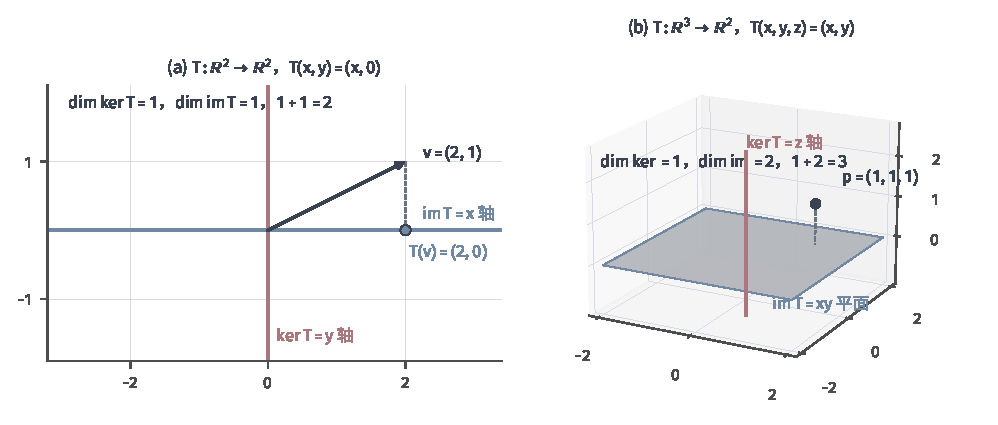
\includegraphics[width=169mm]{figures/00-shared/mathematical-preliminaries-upper/02-linear-spaces/matplotlib/ls-kernel-image-rank-nullity/ls-kernel-image-rank-nullity.pdf}
  \caption{核与像的维数此消彼长。左：$T(x,y)=(x,0)$把平面映到$x$轴，核是$y$轴（红直线）、像是$x$轴（蓝直线），$\dim\ker T=1$、$\dim\operatorname{im}T=1$，$1+1=2$；样本$\bm v=(2,1)$被映到$(2,0)$。右：$T(x,y,z)=(x,y)$把三维空间映到$xy$平面，核是$z$轴（红直线）、像是整个$xy$平面（浅蓝），$\dim\ker T=1$、$\dim\operatorname{im}T=2$，$1+2=3$。两图为解析教学例。}
  \label{fig:ls-kernel-image-rank-nullity}
\end{figure*}

对$\bm A\in\mathbb R^{m\times d}$，$\operatorname{rank}\bm A\leq\min(m,d)$：列空间在$\mathbb R^m$中，维数不超过$m$；它由$d$列张成，从中抽取出的基不超过$d$个向量。$\operatorname{rank}\bm A=d$称为满列秩，这时输入方向全部被保留，等价于各列线性无关；$\operatorname{rank}\bm A=m$称为满行秩，这时输出全部可达；二者统称\term{满秩}（full rank）。

形状不同时，二者不能同时成立。$m<d$时，即使满行秩，核的维数也是$d-m>0$；$m>d$时，即使满列秩，像的维数也只有$d<m$，总有输出无法到达。例如贯穿例$\bm X_\varepsilon$在$\varepsilon\neq0$时两列线性无关（示例~\ref{ex:ls-nearly-collinear-independence}），秩为$2$，满列秩；它的像是$\mathbb R^3$中的一个平面，不是满行秩。

\paragraph{商空间}
前面看到，输出相同的输入恰好彼此相差一个核方向。按输出把输入分组，每组都形如$\bm x+\ker T$，正是第~\ref{sec:ls-quotient-spaces}节取$U=\ker T$得到的等价类，全部分组组成商空间$V/\ker T$。

规则$\bm x+\ker T\mapsto T\bm x$不依赖代表元，因为代表元相差核方向时输出相同。它保持线性组合，满射到$\operatorname{im}T$；它也是单射，因为两个类的像相同即$T\bm x=T\bm y$时，$\bm x-\bm y\in\ker T$，两个类相同。所以它是从$V/\ker T$到$\operatorname{im}T$的线性双射：压去全部丢失方向以后，每个等价类恰对应一个可达输出。线性双射把一组基送到一组基，两边维数相同；由式~\eqref{eq:ls-quotient-dimension}得$\dim V-\dim\ker T=\operatorname{rank}T$，这是秩零度定理的另一种读法。在示例~\ref{ex:ls-kernel-indistinguishable}中，商空间$\mathbb R^4/\ker T$是三维的，像$\mathbb R^3$也是三维的。

\paragraph{矩阵的行空间与列空间}
示例~\ref{ex:ls-rank-one-four-subspaces}中，行空间与列空间维数相同，零空间与行空间的维数之和为输入维数，列空间与左零空间的维数之和为输出维数。现在对一般的$\bm A\in\mathbb R^{m\times d}$证明这些规律。对$\bm A$用秩零度定理，零空间与列空间的维数之和为$d$；对$\bm A^\top$用它，左零空间与行空间的维数之和为$m$。剩下的问题是两个“列空间”之间的关系：行空间与列空间是否总一样大？
\begin{theorem}[行秩等于列秩]
\label{thm:ls-row-rank-column-rank}
对任意$\bm A\in\mathbb R^{m\times d}$，$\dim\operatorname{range}(\bm A^\top)=\dim\operatorname{range}(\bm A)$，即$\operatorname{rank}\bm A^\top=\operatorname{rank}\bm A$。
\end{theorem}
\begin{proof}
设$r=\operatorname{rank}\bm A$，取列空间的一组基$\bm c_1,\ldots,\bm c_r$，排成$\bm C\in\mathbb R^{m\times r}$。$\bm A$的每一列都在列空间中，所以第$j$列可写成$\bm A_{:,j}=\bm C\bm r_j$，$\bm r_j\in\mathbb R^r$；把这些系数列排成$\bm R\in\mathbb R^{r\times d}$，按乘积的列读法得$\bm A=\bm C\bm R$。再按行读这个乘积：$\bm A$的第$i$行是$\bm A_{i,:}=\sum_{k=1}^r\bm C_{i,k}\bm R_{k,:}$，即$\bm R$的$r$行的线性组合。所以$\bm A$的全部行都落在$\bm R$的$r$行张成的空间里，行空间的维数不超过$r$，即$\operatorname{rank}\bm A^\top\leq\operatorname{rank}\bm A$。对$\bm A^\top$用同样的论证，得$\operatorname{rank}\bm A\leq\operatorname{rank}\bm A^\top$，两者相等。
\end{proof}
于是行秩（行空间的维数）与列秩（列空间的维数）可以统称为秩。对$\bm A$与$\bm A^\top$分别用秩零度定理，四个基本子空间的维数全部由$m,d$与$r=\operatorname{rank}\bm A$决定：
\begin{equation}
 \begin{gathered}
 \dim\operatorname{range}(\bm A)=\dim\operatorname{range}(\bm A^\top)=r,\\
 \dim\operatorname{null}(\bm A)=d-r,\qquad
 \dim\operatorname{null}(\bm A^\top)=m-r.
 \end{gathered}
 \label{eq:ls-four-subspace-dimensions}
\end{equation}
输入空间中的零空间与行空间维数相加为$d$，输出空间中的列空间与左零空间维数相加为$m$。

对示例~\ref{ex:ls-rank-one-four-subspaces}中的$\bm A$，$r=1$，式~\eqref{eq:ls-four-subspace-dimensions}给出的维数与直接计算一致；证明中的分解$\bm A=\bm C\bm R$在那里就是$\bm A=(1,2)^\top(1,2,3)$。该示例还显示，两对子空间不仅维数互补，而且互相垂直。这一规律要在第~\ref{sec:ls-orthogonality}节有了内积以后才能说清；第~\ref{sec:ls-dual-map}节还将用对偶映射给出行秩等于列秩的另一个证明。

\subsection{单射、满射与可逆性}
\phantomsection
\label{sec:ls-injective-surjective-invertible}
给定输出，能否唯一还原输入？这个问题分成两半：不同的输入是否给出不同的输出，以及每个输出是否都能被到达。对线性映射，这两半都可以用子空间判断。单射等价于核为零：$T\bm x=T\bm y$当且仅当$\bm x-\bm y\in\ker T$，核为零时输出相同必输入相同；反过来，核中若有非零向量，它与$\bm0$的输出相同，映射就不是单射。满射等价于像等于整个输出空间。有限维时可以用秩零度定理把二者换成维数：单射当且仅当$\operatorname{rank}T=\dim V$，满射当且仅当$\operatorname{rank}T=\dim W$。

输入输出维数相等时，秩零度定理使三种性质合而为一：$\dim V=\dim W$时，$\ker T=\{\bm0\}$等价于$\operatorname{rank}T=\dim V=\dim W$，于是单射、满射、双射互相等价，只需检查其中一条。维数不同时则须分别判断：$\dim V<\dim W$时像的维数至多为$\dim V$，不可能满射；$\dim V>\dim W$时核的维数至少为$\dim V-\dim W>0$，不可能单射。所以只有输入输出维数相等的映射才可能双侧可逆，矩形矩阵即使满秩，也只能是单射或满射之一。

把这些判据与上一小节可逆映射和逆矩阵的对应合起来，对$n$阶方阵$\bm A$，下列条件互相等价：
\[
 \bm A\text{可逆}
 \iff\operatorname{null}(\bm A)=\{\bm0\}
 \iff\operatorname{rank}\bm A=n
 \iff\bm A\text{的}n\text{列线性无关}.
\]
其中第三、四个条件等价，是因为列空间由$n$列张成，维数为$n$恰好说明这$n$列构成它的一组基。由行秩等于列秩，还可以在链中加入“$\bm A$的$n$行线性无关”。第~\ref{sec:ls-determinant-invertibility}节讨论线性方程时，还将用行列式给出一个等价的数值判据$\det\bm A\neq0$。

这一等价还给出第~\ref{sec:ls-square-one-sided-inverse}节“方阵的单侧逆即逆”的另一个证明，不必借助行列式。若$n$阶方阵满足$\bm B\bm A=\bm I_n$，则$\bm A\bm x=\bm0$蕴含$\bm x=\bm B\bm A\bm x=\bm0$，核为零，$\bm A$可逆，于是$\bm B=\bm B\bm A\bm A^{-1}=\bm A^{-1}$；$\bm A\bm B=\bm I_n$时对$\bm B$作同样论证。

同理，若$n$阶方阵的乘积$\bm A\bm B$可逆，则两个因子都可逆。$\bm B\bm x=\bm0$蕴含$\bm A\bm B\bm x=\bm0$，从而$\bm x=\bm0$，$\bm B$的核为零，因而可逆；于是$\bm A=(\bm A\bm B)\bm B^{-1}$是可逆矩阵的乘积，也可逆。

最容易还原的情形是逐坐标缩放；一般的矩阵把坐标掺在一起，但判据相同：核为零且维数相等。
\begin{example}[用核判断可逆]
\label{ex:ls-kernel-invertibility}
给定：对角矩阵$\operatorname{diag}(d_1,\ldots,d_n)$与$\bm A=\left[\begin{smallmatrix}2&1\\0&3\end{smallmatrix}\right]$。

验证：对角矩阵逐坐标缩放，坐标之间互不影响。若每个$d_i\neq0$，逐坐标除以$d_i$即可撤销，逆矩阵为$\operatorname{diag}(1/d_1,\ldots,1/d_n)$。若某个$d_i=0$，相应坐标被压为零，$\bm e_i$落入核中，两个只在第$i$个坐标不同的输入给出相同输出。对$\bm A$，$\bm A\bm x=\bm0$即$2x_1+x_2=0$与$3x_2=0$；第二式给出$x_2=0$，代入第一式得$x_1=0$，所以核为零。

结论：对角矩阵可逆当且仅当全部$d_i\neq0$；$\bm A$是方阵且核为零，所以可逆，它的逆矩阵已在第~\ref{sec:prelim-inverse-matrices}节求出。
\end{example}

\paragraph{单侧逆}
维数不同时，仍可以只撤销一半。单射$T:V\to W$可以找到线性映射$L:W\to V$使$L\circ T=\operatorname{id}_V$：在像上按$T$的逆读回输入，在像的一个补空间上任意规定（例如送到零）。满射$T$可以找到$R:W\to V$使$T\circ R=\operatorname{id}_W$：为输出基中的每个向量任选一个原输入，再线性延拓。补空间与原输入的选法不唯一，所以这些单侧逆一般也不唯一。

写成矩阵，对$\bm A\in\mathbb R^{m\times d}$：$\bm A$有左逆当且仅当它满列秩，有右逆当且仅当它满行秩。充分性来自上面的构造，因为满列秩就是单射，满行秩就是满射。必要性同样直接：若$\bm L\bm A=\bm I_d$，则$\bm A\bm x=\bm0$蕴含$\bm x=\bm L\bm A\bm x=\bm0$，核为零；若$\bm A\bm R=\bm I_m$，则每个$\bm y=\bm A(\bm R\bm y)$都可到达。第~\ref{sec:prelim-inverse-matrices}节的例子$\bm A=(1,0)^\top$满列秩，有无穷多个左逆。多解时如何选择代表，由第~\ref{chap:linear-equations-and-optimization}章回答。

\subsection{换基、矩阵等价与相似}
\label{sec:ls-coordinates-change-of-basis}

第~\ref{sec:ls-coordinates}节看到，同一个对象在不同基下有不同的坐标；同样，同一个线性映射换一组基，记录它的矩阵通常也随之改变。现在坐标变换、矩阵表示与逆矩阵都已齐备，这种变化可以精确写出。本小节回答两个问题：一般线性映射在输入、输出两端各自换基以后，矩阵怎样变化，两个同形矩阵什么时候记录同一个映射；线性算子两端一起换基时，又会怎样。

一般映射放在算子之前。映射的两端是两个空间，可以独立换基，得到的关系称为相抵；算子要求两端使用同一组基，换基时两端必须一起变，相应的关系称为相似，它是相抵加上“两端换基相同”这一约束的特例。约束减少了可用的自由度：相抵只需秩就能完全分类，相似却要更多不变量。

推导要用到一个观察：换基矩阵本身就是一个线性映射的矩阵。比较式~\eqref{eq:linear-algebra-coordinate-change}与式~\eqref{eq:linear-algebra-map-matrix-representation}可见，$\bm S_{\mathcal C\leftarrow\mathcal B}$正是恒等映射$\operatorname{id}_V$在输入基$\mathcal B$、输出基$\mathcal C$下的矩阵：对象不动，只是输入端与输出端用不同的基记录。连续换基的乘法公式，也就是复合公式~\eqref{eq:ls-composition-matrix}对$\operatorname{id}_V\circ\operatorname{id}_V=\operatorname{id}_V$的特例。

\subsubsection{一般线性映射的换基与相抵}
\label{sec:ls-equivalence-matrices}

设$T:V\to W$是线性映射，$\dim V=d$、$\dim W=m$。它在一对基下记录为矩阵$\bm A$，在另一对基下记录为$\bm B$，$\bm A$与$\bm B$有什么关系？反过来，两个同形矩阵什么时候记录的是同一个映射？

\paragraph{换基过程}
设$\mathcal B,\mathcal B'$是$V$的两组基，$\mathcal C,\mathcal C'$是$W$的两组基，记$\bm A=[T]_{\mathcal C\leftarrow\mathcal B}$、$\bm B=[T]_{\mathcal C'\leftarrow\mathcal B'}$，输入端换基矩阵$\bm P=\bm S_{\mathcal B\leftarrow\mathcal B'}$（$d$阶可逆），输出端换基矩阵$\bm Q=\bm S_{\mathcal C\leftarrow\mathcal C'}$（$m$阶可逆）。$\bm P$的第$j$列是新输入基向量在旧输入基下的坐标，$\bm Q$同理。已知新输入坐标$[\bm v]_{\mathcal B'}$，求新输出坐标$[T\bm v]_{\mathcal C'}$，可以绕道旧基分三步完成。

第一步，把新输入坐标换成旧输入坐标：$[\bm v]_{\mathcal B}=\bm P[\bm v]_{\mathcal B'}$。第二步，在旧基下作用：$[T\bm v]_{\mathcal C}=\bm A[\bm v]_{\mathcal B}=\bm A\bm P[\bm v]_{\mathcal B'}$。第三步，把旧输出坐标换成新输出坐标，这要用反向换基矩阵$\bm Q^{-1}=\bm S_{\mathcal C'\leftarrow\mathcal C}$：
\[
 [T\bm v]_{\mathcal C'}=\bm Q^{-1}[T\bm v]_{\mathcal C}=\bm Q^{-1}\bm A\bm P[\bm v]_{\mathcal B'}.
\]
另一方面，按定义$[T\bm v]_{\mathcal C'}=\bm B[\bm v]_{\mathcal B'}$。两式对每个$\bm v$成立；取$\bm v=\bm b'_j$，其新坐标为$\bm e_j$，两边读出的是两个矩阵的第$j$列，所以
\begin{equation}
 \bm B=\bm Q^{-1}\bm A\bm P.
 \label{eq:ls-equivalence-transform}
\end{equation}
从右向左读：$\bm P$把新输入坐标译成旧坐标，$\bm A$在旧基下作用，$\bm Q^{-1}$把结果译成新输出坐标。用复合的语言说，$T=\operatorname{id}_W\circ T\circ\operatorname{id}_V$，三个因子分别在相应的基下记录，由式~\eqref{eq:ls-composition-matrix}就是上式右端的三个矩阵。

\paragraph{相抵的定义}
\phantomsection
\label{sec:ls-equivalence-meaning}
上面的推导说明，同一映射的两个记录之间只相差两侧各乘一个可逆矩阵。反过来，两侧任意乘上可逆矩阵，得到的是否仍是同一映射的记录？先把这种关系单独命名。
\begin{definition}[矩阵相抵]
\label{def:ls-matrix-equivalence}
设$\bm A,\bm B\in\mathbb R^{m\times d}$。若存在可逆矩阵$\bm Q\in\mathbb R^{m\times m}$与$\bm P\in\mathbb R^{d\times d}$使$\bm B=\bm Q^{-1}\bm A\bm P$，就称$\bm A$与$\bm B$\term{相抵}（equivalent matrices）。
\end{definition}
定义中的$\bm Q,\bm P$可以是任意可逆矩阵，不必事先知道它们来自哪组基；写成$\bm Q^{-1}$只是为了与换基推导一致，$\bm Q$取遍全部可逆矩阵时$\bm Q^{-1}$也取遍全部可逆矩阵。

相抵恰好刻画“记录同一个映射”。一个方向已由换基推导给出。另一方向，设$\bm A=[T]_{\mathcal C\leftarrow\mathcal B}$，任给可逆的$\bm P,\bm Q$。由第~\ref{sec:ls-coordinates}节，以$\bm P$的各列为旧基坐标可以得到$V$的一组新基$\mathcal B'$，使$\bm S_{\mathcal B\leftarrow\mathcal B'}=\bm P$；输出端用$\bm Q$同样构造$\mathcal C'$。由换基推导，$T$在这两组新基下的矩阵恰为$\bm Q^{-1}\bm A\bm P$。所以两个同形矩阵相抵，当且仅当它们是同一个线性映射在两端不同选基下的记录。右乘$\bm P$对应输入基的更换，左乘$\bm Q^{-1}$对应输出基的更换；初等列变换与初等行变换分别是这两种换基的具体实现。

\paragraph{相抵不变量}
\phantomsection
\label{sec:ls-equivalence-properties}
既然相抵的矩阵记录同一个映射，映射本身的性质就不应随基改变。哪些量是这样的不变量？相抵首先是等价关系：自反取$\bm Q=\bm P=\bm I$；对称由$\bm A=\bm Q\bm B\bm P^{-1}=(\bm Q^{-1})^{-1}\bm B\bm P^{-1}$；传递由$\bm C=\bm Q_2^{-1}\bm B\bm P_2=(\bm Q_1\bm Q_2)^{-1}\bm A(\bm P_1\bm P_2)$。三条分别对应不换基、换回原基和连续换两次基。

零空间在输入端被搬运：$\bm B\bm x=\bm0$当且仅当$\bm A(\bm P\bm x)=\bm0$，所以$\operatorname{null}(\bm B)=\bm P^{-1}\operatorname{null}(\bm A)$。列空间在输出端被搬运：$\bm B\bm x=\bm Q^{-1}\bm A(\bm P\bm x)$，而$\bm P\bm x$取遍全部输入，所以$\operatorname{range}(\bm B)=\bm Q^{-1}\operatorname{range}(\bm A)$。可逆矩阵把线性无关组送到线性无关组，搬运不改变子空间的维数，因此
\begin{equation}
\begin{gathered}
\operatorname{rank}\bm B=\operatorname{rank}\bm A\\
\dim\operatorname{null}(\bm B)=\dim\operatorname{null}(\bm A)=d-\operatorname{rank}\bm A.
\end{gathered}
\label{eq:ls-equivalence-invariants}
\end{equation}
相抵允许的记录变化很宽：输入与输出可以是不同空间，$\bm B$一般不是方阵，不能对自身反复作用，所以幂、迹这类只对算子有意义的量不在讨论之列。

\paragraph{秩标准形与相抵判据}
\phantomsection
\label{sec:ls-equivalence-conditions}
秩是相抵不变量；反过来，秩相同的两个同形矩阵是否一定相抵？答案是肯定的。办法是说明两端可以独立选基时，每个矩阵都能化成只由秩决定的简单形状。

设$\bm A$是$T$在某对基下的矩阵，$r=\operatorname{rank}\bm A$。取$\ker T$的一组基并扩充为$V$的基，由秩零度定理，新增向量恰有$r$个，把它们排在前面。这$r$个向量的像线性无关：若像的某个组合为零，相应的新增向量组合就落进核，能由核的基表示，整组基的线性无关性迫使系数全为零。

核的基向量的像都是零，所以这$r$个像还张成$\operatorname{im}T$。再把这$r$个像扩充为$W$的基。在这样选取的两组基下，$T$把前$r$个输入基向量依次送到前$r$个输出基向量，其余输入基向量送到零，矩阵为秩标准形
\begin{equation}
\begin{gathered}
\begin{bmatrix}\bm I_r&\bm0\\\bm0&\bm0\end{bmatrix}\\
r=\operatorname{rank}\bm A.
\end{gathered}
\label{eq:ls-rank-normal-form}
\end{equation}

下面对一个秩为$1$的二阶矩阵具体做出这两组基。
\begin{example}[两端各自选基化为秩标准形]
\label{ex:ls-rank-normal-form-two-by-two}
给定：$\bm A=\left[\begin{smallmatrix}1&2\\2&4\end{smallmatrix}\right]$，$T\bm x=\bm A\bm x$，两端原来都用标准基。

计算：两列共线，$\operatorname{rank}\bm A=1$；$\bm A(-2,1)^\top=\bm0$，所以$\ker T=\operatorname{span}\{(-2,1)^\top\}$。输入端取$\bm v_1=\bm e_1$与核中的$\bm v_2=(-2,1)^{\top}$，输出端取$\bm w_1=\bm A\bm v_1=(1,2)^{\top}$并补上$\bm w_2=\bm e_2$。以新基向量的标准坐标为列，
\[
\begin{gathered}
\bm P=\begin{bmatrix}1&-2\\0&1\end{bmatrix}\\
\bm Q=\begin{bmatrix}1&0\\2&1\end{bmatrix}\\
\bm Q^{-1}=\begin{bmatrix}1&0\\-2&1\end{bmatrix}.
\end{gathered}
\]
先算$\bm A\bm P=\left[\begin{smallmatrix}1&0\\2&0\end{smallmatrix}\right]$，再左乘$\bm Q^{-1}$：
\[
 \bm Q^{-1}\bm A\bm P=\begin{bmatrix}1&0\\-2&1\end{bmatrix}\begin{bmatrix}1&0\\2&0\end{bmatrix}
 =\begin{bmatrix}1&0\\0&0\end{bmatrix}.
\]

结论：在新基下，$T$把$\bm v_1$送到$\bm w_1$，把核方向$\bm v_2$送到零，矩阵为秩标准形$\operatorname{diag}(1,0)$。
\end{example}
图~\ref{fig:ls-equivalence-two-sided-bases-flow}画出这两组基：$\bm v_1$被送到$\bm w_1$，核方向$\bm v_2$被送到零，输出端的$\bm w_2$不被任何输入到达。两端各自选基，才能同时做到这两件事；若要求两端用同一组基，这一化简一般做不到。
\begin{figure}[!htb]
  \centering
  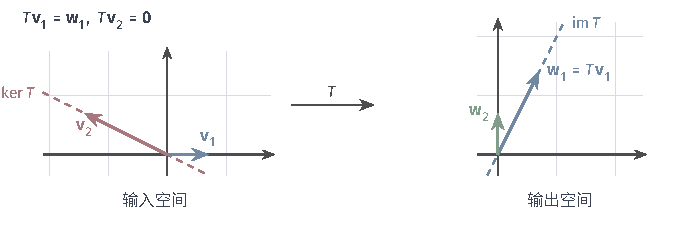
\includegraphics[width=112mm]{figures/00-shared/mathematical-preliminaries-upper/02-linear-spaces/tikz/comprehension-additions/equivalence-two-bases.pdf}
  \caption{两端独立选基化为秩标准形。$T(\bm x)=\bm A\bm x$，$\bm A=\left[\begin{smallmatrix}1&2\\2&4\end{smallmatrix}\right]$。左：输入基$\bm v_1=\bm e_1$（蓝）与$\bm v_2=(-2,1)^{\top}$（红），$\bm v_2$在核（红虚线）上。右：输出基$\bm w_1=T\bm v_1=(1,2)^{\top}$（蓝）位于像（蓝虚线）上，$\bm w_2=\bm e_2$（绿）补足一组基。在这两组基下$T$的矩阵为$\operatorname{diag}(1,0)$。}
  \label{fig:ls-equivalence-two-sided-bases-flow}
\end{figure}

\begin{theorem}[相抵判据]
\label{thm:ls-equivalence-criterion}
两个同形实矩阵$\bm A,\bm B\in\mathbb R^{m\times d}$相抵，当且仅当$\operatorname{rank}\bm A=\operatorname{rank}\bm B$。
\end{theorem}
\begin{proof}
必要性由式\eqref{eq:ls-equivalence-invariants}得到。充分性：设二者秩都为$r$，由上面的构造，存在可逆矩阵使$\bm R=\bm Q_A^{-1}\bm A\bm P_A=\bm Q_B^{-1}\bm B\bm P_B$，其中$\bm R$是式\eqref{eq:ls-rank-normal-form}的秩标准形。两式对接得$\bm B=(\bm Q_A\bm Q_B^{-1})^{-1}\bm A(\bm P_A\bm P_B^{-1})$，即二者相抵。
\end{proof}
所以固定形状以后，秩就是相抵的完整不变量：零矩阵只与零矩阵相抵，同形的满秩矩阵彼此相抵。把矩阵化到标准形的具体消元算法在第~\ref{chap:linear-equations-and-optimization}章建立。

\subsubsection{线性算子的换基与相似}
\label{sec:ls-similarity}
\phantomsection
\label{sec:ls-matrix-equivalences}

线性算子$T:V\to V$的输入与输出是同一个空间，记录时两端用同一组基；换基时，两端必须换成同一组新基。上面的推导加上这个约束会给出什么关系？同一个算子的两个方阵记录什么时候可以互相转化？

\paragraph{换基过程}
设$\mathcal B$与$\mathcal B'$是$V$的两组基，$\bm A=[T]_{\mathcal B}$、$\bm B=[T]_{\mathcal B'}$，记$\bm P=\bm S_{\mathcal B\leftarrow\mathcal B'}$，它的第$j$列是新基向量$\bm b'_j$在旧基$\mathcal B$下的坐标，$\bm P$可逆，反向换基矩阵为$\bm P^{-1}$。输入端与输出端是同一个空间、同一次换基，所以三步推导中的$\bm Q$也是$\bm P$：先把新坐标换成旧坐标，$[\bm v]_{\mathcal B}=\bm P[\bm v]_{\mathcal B'}$；在旧基下作用，$[T\bm v]_{\mathcal B}=\bm A\bm P[\bm v]_{\mathcal B'}$；再把输出换回新坐标，
\[
 [T\bm v]_{\mathcal B'}=\bm P^{-1}[T\bm v]_{\mathcal B}=\bm P^{-1}\bm A\bm P[\bm v]_{\mathcal B'}.
\]
与$[T\bm v]_{\mathcal B'}=\bm B[\bm v]_{\mathcal B'}$逐列比较，得到
\begin{equation}
 \bm B=\bm P^{-1}\bm A\bm P.
 \label{eq:linear-algebra-similarity-change-basis}
\end{equation}
这就是式~\eqref{eq:ls-equivalence-transform}取$\bm Q=\bm P$的情形。

\paragraph{相似的定义}
\phantomsection
\label{sec:ls-similarity-meaning}
与相抵一样，把同一算子两个记录之间的关系单独命名。
\begin{definition}[矩阵相似]
\label{def:ls-matrix-similarity}
设$\bm A,\bm B$是$n$阶方阵。若存在$n$阶可逆矩阵$\bm P$使$\bm B=\bm P^{-1}\bm A\bm P$，就称$\bm A$与$\bm B$\term{相似}（similar）。
\end{definition}
相似的两个矩阵正是同一个线性算子在两组基下的记录。一个方向由上面的推导给出；另一方向，给定$\bm A=[T]_{\mathcal B}$和可逆$\bm P$，以$\bm P$的各列为旧基坐标得到一组新基，$T$在其下的矩阵恰为$\bm P^{-1}\bm A\bm P$。

相似不要求$\bm A,\bm B$本身可逆，可逆的只是换基矩阵$\bm P$。取$\bm Q=\bm P$可见，相似的矩阵必定相抵；反之不然，下面的判定会给出秩相同、因而相抵却不相似的例子。

看一个具体例子：适当换基，可以把一个算子的矩阵化成对角形。
\begin{example}[换基把算子的矩阵化为对角形]
\label{ex:ls-similarity-diagonal}
给定：示例~\ref{ex:ls-plane-operator-matrix}中的算子$T(x_1,x_2)=(2x_1+x_2,3x_2)$，它在标准基下的矩阵为$\bm A=\left[\begin{smallmatrix}2&1\\0&3\end{smallmatrix}\right]$，即$T\bm e_1=2\bm e_1$、$T\bm e_2=\bm e_1+3\bm e_2$；新基取$\bm b_1'=\bm e_1$、$\bm b_2'=\bm e_1+\bm e_2$。

计算：$\bm P=\left[\begin{smallmatrix}1&1\\0&1\end{smallmatrix}\right]$，$\bm P^{-1}=\left[\begin{smallmatrix}1&-1\\0&1\end{smallmatrix}\right]$，
\[
 \bm B=\bm P^{-1}\bm A\bm P
 =\begin{bmatrix}1&-1\\0&1\end{bmatrix}
 \begin{bmatrix}2&1\\0&3\end{bmatrix}
 \begin{bmatrix}1&1\\0&1\end{bmatrix}
 =\begin{bmatrix}2&0\\0&3\end{bmatrix}.
\]
直接验证也是如此：$T\bm b_1'=2\bm b_1'$，$T\bm b_2'=T\bm e_1+T\bm e_2=3\bm e_1+3\bm e_2=3\bm b_2'$。

结论：在新基下，$T$的矩阵是对角矩阵$\operatorname{diag}(2,3)$；两个新基方向在$T$的作用下都只被伸缩、不被转向，彼此互不干扰。
\end{example}
$T$本身没有改变，改变的只是沿哪两条方向读取。图~\ref{fig:ls-similarity-change-of-basis-flow}把这一点画在平面上：在标准基下，单位正方形被$T$拉成一个斜的平行四边形，矩阵$\bm A$有非零的非对角元；在新基下，基向量围成的平行四边形只沿两条基方向分别伸长$2$倍和$3$倍，矩阵就是对角的$\bm B$。只被伸缩的方向称为特征方向；怎样系统地找到它们，什么时候能找到足够多的这种方向组成一组基，是第~\ref{chap:linear-analysis}章的问题。
\begin{figure}[!htb]
  \centering
  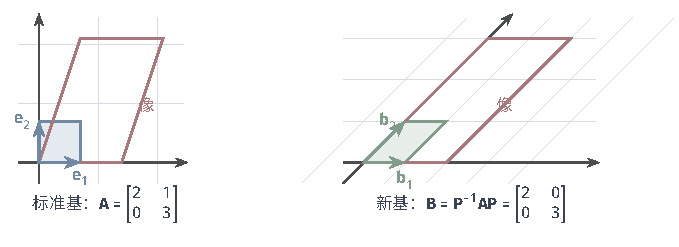
\includegraphics[width=112mm]{figures/00-shared/mathematical-preliminaries-upper/02-linear-spaces/tikz/comprehension-additions/similarity-two-bases.pdf}
  \caption{同一个算子在两组基下的记录。左：标准基$\bm e_1,\bm e_2$围成的单位正方形（蓝）被$\bm A=\left[\begin{smallmatrix}2&1\\0&3\end{smallmatrix}\right]$送到红色平行四边形，形状被斜切。右：新基$\bm b_1=\bm e_1$、$\bm b_2=\bm e_1+\bm e_2$围成的平行四边形（绿）被同一个算子送到红色平行四边形，只沿$\bm b_1$伸长$2$倍、沿$\bm b_2$伸长$3$倍，因此新矩阵为$\operatorname{diag}(2,3)$。浅色斜线为新基网格。}
  \label{fig:ls-similarity-change-of-basis-flow}
\end{figure}

\paragraph{相似不变量}
\phantomsection
\label{sec:ls-similarity-properties}
同一个算子的性质不应随基改变；哪些量在相似下保持不变？相似首先是等价关系：$\bm A=\bm I^{-1}\bm A\bm I$给出自反性；由$\bm B=\bm P^{-1}\bm A\bm P$得$\bm A=\bm P\bm B\bm P^{-1}$，给出对称性；若再有$\bm C=\bm Q^{-1}\bm B\bm Q$，则$\bm C=(\bm P\bm Q)^{-1}\bm A(\bm P\bm Q)$，给出传递性。这三条分别对应不换基、换回原基和连续换两次基。

相似是相抵的特例，相抵不变量自然保持：$\operatorname{null}(\bm B)=\bm P^{-1}\operatorname{null}(\bm A)$，$\operatorname{range}(\bm B)=\bm P^{-1}\operatorname{range}(\bm A)$，因此
\begin{equation}
\begin{gathered}
\operatorname{rank}\bm B=\operatorname{rank}\bm A\\
\dim\operatorname{null}(\bm B)=\dim\operatorname{null}(\bm A).
\end{gathered}
\label{eq:ls-similarity-invariants}
\end{equation}
算子还能反复作用，而先后作用与换基相容：若$\bm B_1=\bm P^{-1}\bm A_1\bm P$、$\bm B_2=\bm P^{-1}\bm A_2\bm P$，则
\begin{equation}
 \bm B_1\bm B_2
 =\bm P^{-1}\bm A_1\bm P\,\bm P^{-1}\bm A_2\bm P
 =\bm P^{-1}\bm A_1\bm A_2\bm P,
 \label{eq:ls-similarity-product}
\end{equation}
中间的$\bm P\bm P^{-1}$相消。归纳得$\bm B^k=\bm P^{-1}\bm A^k\bm P$：反复作用同一个算子，在新基下仍是同一过程的记录。同样，对任意实数$c$，$\bm B-c\bm I=\bm P^{-1}(\bm A-c\bm I)\bm P$，所以$\bm A-c\bm I$与$\bm B-c\bm I$也相似，由式~\eqref{eq:ls-similarity-invariants}，
\begin{equation}
\begin{gathered}
\operatorname{rank}(\bm B-c\bm I)=\operatorname{rank}(\bm A-c\bm I)\\
c\in\mathbb R.
\end{gathered}
\label{eq:ls-similarity-shifted-rank}
\end{equation}
这比总秩更细：它对每个$c$都给出一个不变量。

相似还保持两个可以直接计算的标量。由行列式的乘法性（第~\ref{sec:ls-determinant-properties}节）与$\det(\bm P^{-1})\det\bm P=\det\bm I=1$，
\[
 \det(\bm P^{-1}\bm A\bm P)=\det(\bm P^{-1})\,\det\bm A\,\det\bm P=\det\bm A;
\]
由迹的循环性（式~\eqref{eq:linear-algebra-trace-cyclic}），
\[
 \operatorname{tr}(\bm P^{-1}\bm A\bm P)=\operatorname{tr}\bigl((\bm A\bm P)\bm P^{-1}\bigr)=\operatorname{tr}\bm A.
\]
两式说明，行列式与迹只依赖算子本身，是判断两个矩阵能否记录同一算子时可以直接计算的两个标量不变量。例如示例~\ref{ex:ls-similarity-diagonal}中的$\bm A$与$\bm B=\operatorname{diag}(2,3)$行列式都是$6$，迹都是$5$。于是可以说“算子$T$的行列式”“算子$T$的迹”，用任意一组基下的矩阵计算即可。

引入特征值以后还将看到（第~\ref{sec:ls-eigen-similarity-invariance}节），特征值与特征多项式同样是相似不变量，而行列式与迹恰好是特征值之积与特征值之和。一般的换基不保持欧氏长度与夹角，这些度量量不在相似保持之列。

\paragraph{相似的判定}
\phantomsection
\label{sec:ls-similarity-conditions}
怎样判断两个给定的方阵是否相似？两端左乘$\bm P$，相似等价于存在\emph{可逆}的$\bm P$满足
\begin{equation}
 \bm A\bm P=\bm P\bm B.
 \label{eq:ls-similarity-equation}
\end{equation}
这是关于$\bm P$各元素的一组线性方程。只找到非零但不可逆的解还不够：那只是两个坐标子空间之间的对应，不是两组基之间的换基。

不变量给出否定的判据：只要某个相似不变量不同，两个矩阵就不相似。但秩、行列式、迹相同，都只是相似的必要条件，下面的例子说明它们合在一起也不够。
\begin{example}[反例：相抵而不相似的两个矩阵]
\label{ex:ls-equivalent-not-similar}
给定：$\bm I_2$与$\bm J=\left[\begin{smallmatrix}1&1\\0&1\end{smallmatrix}\right]$。

验证：二者都可逆，秩都为$2$，由相抵判据它们相抵；二者的行列式都是$1$，迹都是$2$。但取$c=1$，$\bm I_2-\bm I_2=\bm0$的秩为$0$，而$\bm J-\bm I_2=\left[\begin{smallmatrix}0&1\\0&0\end{smallmatrix}\right]$的秩为$1$，式~\eqref{eq:ls-similarity-shifted-rank}不成立。更直接地，若$\bm J=\bm P^{-1}\bm I_2\bm P$，则$\bm J=\bm P^{-1}\bm P=\bm I_2$，矛盾。

结论：$\bm I_2$与$\bm J$相抵，秩、行列式与迹也都相同，却不相似；单位矩阵只与自己相似。
\end{example}
这正是“两端换基相同”这一约束的代价：相抵时秩相同就足够，相似时连秩、行列式与迹一起相同都不够。比较$\bm A-c\bm I$在各个$c$处的秩是更细的必要条件；完整的相似分类需要Jordan标准形，本书不展开。

\subsection{多线性映射}

此前的线性映射只有一个输入。矩阵的元素内积、两个向量的外积却各有两个输入：固定其中一个，再改变另一个时，结果保持线性组合。为了表达这种逐个输入的线性，可以为每个输入保留一个独立的槽位。

设$V_1,\ldots,V_k,W$是同一数域上的线性空间。映射$F:V_1\times\cdots\times V_k\to W$若在固定其余输入后，对每一个输入分别都是线性的，就称为多线性映射；$k=2$时称为双线性映射。例如$F(\bm x,\bm y)=\bm x\bm y^\top$对两个输入分别线性。

分别线性不等于把输入对看成一个整体以后仍线性：对实数乘法$f(x,y)=xy$，有$f(1,1)+f(1,1)=2$，但$f(2,2)=4$。

各输入空间和输出空间选定基后，多线性映射也能由有限组系数记录。以实双线性标量映射$B:V\times W\to\mathbb R$为例，取基$(\bm v_i)$与$(\bm w_j)$，令$b_{i,j}=B(\bm v_i,\bm w_j)$。当$\bm x=\sum_i x_i\bm v_i$、$\bm y=\sum_j y_j\bm w_j$时，逐个槽位展开得到
\[
 B(\bm x,\bm y)=\sum_{i,j}x_i y_j b_{i,j}.
\]
因此，基向量两两配对的结果足以恢复任意输入的值。换基改变这些系数，映射本身不变；它与上一章数组的张量积和指标收缩有关，但不能把改变数组存放次序直接等同于改变坐标基。

% 第5章第4节：对偶空间（线性泛函与对偶空间、对偶基、对偶映射与转置）。

\section{对偶空间}
\label{sec:ls-dual-spaces}

线性映射把对象送到另一个空间；还有一类最简单的作用，只把对象读成一个数。取多项式在某一点的值、取信号的第一个样本、计算一组特征的加权和，都是这样的读取；第~\ref{sec:ls-coordinates}节的坐标$x_j$也是，每个坐标都把对象读成一个数。第~\ref{chap:linear-operations}章在$\mathbb R^d$上用内积$\langle\bm w,\bm x\rangle$表示加权读取，读取规则借一个向量$\bm w$来写；一般空间上还没有内积，读取规则本身是什么对象，就需要单独回答。

本节讨论三个问题：全部线性读取组成怎样的空间；坐标作为读取，与基有怎样的关系；对象经过线性映射以后，输出端的读取怎样传回输入端。最后一个问题的答案是转置，它给第~\ref{chap:linear-operations}章中“行列互换”的操作一个不依赖坐标的含义。回答这三个问题只用到线性运算；读取规则的大小需要范数，留到下一章讨论。

\subsection{线性泛函与对偶基}
\label{sec:ls-dual-space}

\paragraph{线性泛函}
保持线性组合的标量读取称为\term{线性泛函}（linear functional）：映射$\varphi:V\to\mathbb R$满足
\[
\begin{gathered}
\varphi(a\bm x+b\bm y)=a\varphi(\bm x)+b\varphi(\bm y)\\
\bm x,\bm y\in V,\ a,b\in\mathbb R.
\end{gathered}
\]
它就是陪域为$\mathbb R$的线性映射。在$P_k$上，取值$p\mapsto p(t_0)$与积分$p\mapsto\int_0^1p(t)\,\mathrm dt$都是线性泛函；在$\mathbb R^d$上，读取第$j$个坐标与加权和$\bm x\mapsto\bm a^\top\bm x$都是线性泛函。但并非每个把向量读成一个数的规则都是线性泛函。
\begin{example}[反例：两个非线性的读取]
\label{ex:ls-nonlinear-readouts}
给定：$\mathbb R^d$上的两个读取$\varphi_1(\bm x)=x_1+1$与$\varphi_2(\bm x)=\lVert\bm x\rVert_2$。

验证：线性泛函必把零向量读成$0$，而$\varphi_1(\bm0)=1$。线性泛函还满足$\varphi(-\bm x)=-\varphi(\bm x)$；但对任一$\bm x\neq\bm0$，$\varphi_2(-\bm x)=\lVert\bm x\rVert_2>0$，而$-\varphi_2(\bm x)<0$。

结论：$\varphi_1$与$\varphi_2$都不是线性泛函。
\end{example}

按线性映射的矩阵表示，选定$V$的基$\mathcal B=(\bm b_1,\ldots,\bm b_d)$、输出端取数$1$作基，线性泛函$\varphi$记录为$1\times d$矩阵
\[
 \begin{gathered}
[\varphi]_{\mathcal B}=\bigl(\varphi(\bm b_1),\ \ldots,\ \varphi(\bm b_d)\bigr)\\
\varphi(\bm v)=[\varphi]_{\mathcal B}[\bm v]_{\mathcal B}=\sum_{j=1}^dx_j\varphi(\bm b_j).
 \end{gathered}
\]
对象的坐标是一列，读取规则的系数是一行，二者相乘得到读数。

非零泛函取到某个非零值，把相应的输入缩放即可取到任意实数，所以它的像是整个$\mathbb R$；由秩零度定理，它的核是$d-1$维子空间。读数等于$c$的点组成核的平移$\bm x_0+\ker\varphi$（其中$\varphi(\bm x_0)=c$），在平面上就是一族平行直线。

\paragraph{对偶空间}
同一个对象可以接受多种读取，两种读取也可以组合：规定
\[
 (\alpha\varphi+\beta\psi)(\bm x)=\alpha\varphi(\bm x)+\beta\psi(\bm x),
\]
右端对$\bm x$仍保持线性组合，所以线性泛函的线性组合仍是线性泛函。全部线性泛函在这两种运算下构成线性空间，称为$V$的\term{对偶空间}（dual space），记为$V^*$。输入向量是被读取的对象，泛函是读取规则，二者属于不同的空间；即使在$\mathbb R^d$中一行系数与一列坐标的数字相同，也不能直接相加。

\paragraph{对偶基}
$V^*$有多大？坐标给出了一组现成的读取。对$V$的有序基$\mathcal B=(\bm b_1,\ldots,\bm b_d)$，第$j$个坐标$\bm v\mapsto x_j$是线性泛函（坐标映射保持线性组合），记为$\varphi_j$。由$\bm b_i$的坐标是$\bm e_i$，
\begin{equation}
 \varphi_j(\bm b_i)=\delta_{j,i}
 =\begin{cases}1,&i=j,\\0,&i\neq j.\end{cases}
 \label{eq:ls-dual-basis-def}
\end{equation}
反过来，线性泛函由它在基向量上的值决定，所以式~\eqref{eq:ls-dual-basis-def}也可以当作$\varphi_j$的定义。

这$d$个读取构成$V^*$的一组基。任意$\varphi\in V^*$都能写成
\[
 \varphi=\sum_{j=1}^d\varphi(\bm b_j)\,\varphi_j,
\]
因为两边在每个$\bm b_i$上取值都是$\varphi(\bm b_i)$，而线性泛函由基向量上的值决定。

若$\sum_ja_j\varphi_j=0$，在$\bm b_i$上取值得$a_i=0$，所以它们线性无关。这组$\varphi_1,\ldots,\varphi_d$称为$\mathcal B$的\term{对偶基}（dual basis），于是$\dim V^*=\dim V$。读取$\varphi$在对偶基下的坐标正是它在各基向量上的读数$\varphi(\bm b_j)$，即上面那一行系数。

对偶基的每个成员依赖整组基，而不只依赖对应的那个基向量。
\begin{example}[改变第二个基向量会改变第一个坐标读取]
\label{ex:ls-dual-basis-depends-on-basis}
给定：$\mathbb R^2$的标准基$(\bm e_1,\bm e_2)$与基$(\bm e_1,\bm e_1+\bm e_2)$。

计算：标准基的对偶基是两个坐标读取$\varphi_1(x,y)=x$、$\varphi_2(x,y)=y$。在第二组基下，
\[
 (x,y)^\top=(x-y)\bm e_1+y(\bm e_1+\bm e_2),
\]
所以第一个坐标读取变成$x-y$，第二个坐标读取仍是$y$。

结论：两组基的第一个向量都是$\bm e_1$，相应的第一个对偶读取却从$x$变成了$x-y$。
\end{example}
对一般的基，对偶基要由方程组$\varphi_j(\bm b_i)=\delta_{j,i}$解出。
\begin{example}[斜基的对偶基]
\label{ex:ls-dual-basis-oblique}
给定：$\mathbb R^2$的基$\bm b_1=(2,1)^\top$、$\bm b_2=(-1,1)^\top$，以及读取横坐标的泛函$\ell(x,y)=x$。

计算：设$\varphi_1(x,y)=\alpha x+\beta y$。条件$\varphi_1(\bm b_1)=2\alpha+\beta=1$与$\varphi_1(\bm b_2)=-\alpha+\beta=0$给出$\alpha=\beta=1/3$；同样由$\varphi_2(\bm b_1)=0$、$\varphi_2(\bm b_2)=1$解出$\varphi_2$，得
\[
 \begin{gathered}
\varphi_1(x,y)=\frac{x+y}3\\
\varphi_2(x,y)=\frac{-x+2y}3 .
 \end{gathered}
\]
$\ell$在基向量上的读数为$\ell(\bm b_1)=2$、$\ell(\bm b_2)=-1$，所以$\ell=2\varphi_1-\varphi_2$。代入验证：$\tfrac23(x+y)-\tfrac13(-x+2y)=x$。

结论：$\ell$在对偶基下的坐标是$(2,-1)$，正是它在两个基向量上的读数。
\end{example}
图~\ref{fig:ls-dual-basis-readout}画出这些读取：每个对偶读取只在一个基向量上读到$1$，在另一个基向量上读到$0$。
\begin{figure}[htbp]
  \centering
  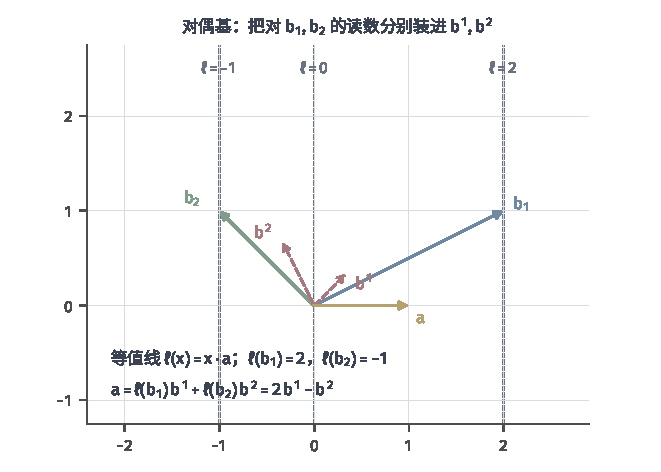
\includegraphics[width=112mm]{figures/00-shared/mathematical-preliminaries-upper/02-linear-spaces/matplotlib/ls-dual-basis-readout/ls-dual-basis-readout.pdf}
  \caption{对偶读取的几何示意。蓝箭头$\bm b_1=(2,1)$、绿箭头$\bm b_2=(-1,1)$为基向量；红色虚线箭头$\bm b^1=(1/3,1/3)$、$\bm b^2=(-1/3,2/3)$分别是对偶基$\varphi_1,\varphi_2$的系数向量，即$\varphi_i(\bm x)=\bm b^i\cdot\bm x$，满足$\varphi_i(\bm b_j)=\delta_{i,j}$。把读取规则画成平面箭头借用了标准内积，这一对应在第~\ref{sec:ls-riesz-representation}节说明。黄色箭头$\bm a=(1,0)$给出读取$\ell(\bm x)=\bm a\cdot\bm x$，灰色虚线为等值线$\ell=c$（$c=-1,0,2$）；$\ell(\bm b_1)=2$、$\ell(\bm b_2)=-1$，且$\bm a=2\bm b^1-\bm b^2$。}
  \label{fig:ls-dual-basis-readout}
\end{figure}

换基时，读取系数与坐标的变化方向相反。

设新基$\mathcal B'$由换基矩阵$\bm P=\bm S_{\mathcal B\leftarrow\mathcal B'}$给出，即$\bm b'_j=\sum_i\bm P_{i,j}\bm b_i$。坐标按$[\bm v]_{\mathcal B'}=\bm P^{-1}[\bm v]_{\mathcal B}$变化；读取系数则按$\varphi(\bm b'_j)=\sum_i\varphi(\bm b_i)\bm P_{i,j}$变化，即$[\varphi]_{\mathcal B'}=[\varphi]_{\mathcal B}\bm P$。二者相乘时$\bm P$与$\bm P^{-1}$相消，读数$\varphi(\bm v)$不随基改变，这正是读数应有的性质。

\subsection{对偶映射}
\label{sec:ls-dual-map}

已知线性映射$T:V\to W$和输出端的一个读取$f\in W^*$，输入$\bm x$经过$T$以后被读成$f(T\bm x)$。先作用、再读取，合起来是输入端的一个读取。由这一复合定义\term{对偶映射}（dual map）$T':W^*\to V^*$：
\begin{equation}
\begin{gathered}
T'f=f\circ T\\
(T'f)(\bm x)=f(T\bm x).
\end{gathered}
\label{eq:ls-dual-map-def}
\end{equation}
$T'$保持线性组合：$(T'(\alpha f+\beta g))(\bm x)=\alpha f(T\bm x)+\beta g(T\bm x)$。对象从$V$走到$W$，读取则从$W^*$传回$V^*$，方向相反；这只是把读取规则搬回输入端，并不是对$T$求逆。复合时次序也随之反转：对$S:W\to U$，$(S\circ T)'f=f\circ S\circ T=T'(S'f)$，即$(S\circ T)'=T'\circ S'$。

\paragraph{对偶映射的矩阵是转置}
设输入基$\mathcal B=(\bm b_1,\ldots,\bm b_d)$、输出基$\mathcal C=(\bm c_1,\ldots,\bm c_m)$下$T$的矩阵为$\bm A$，即$T\bm b_j=\sum_ka_{k,j}\bm c_k$；两组基的对偶基分别记为$\varphi_1,\ldots,\varphi_d$与$\psi_1,\ldots,\psi_m$。取输出读取$f=\sum_iy_i\psi_i$，它传回输入端以后，在输入基向量上的读数是
\[
 (T'f)(\bm b_j)=f(T\bm b_j)
 =\sum_iy_i\,\psi_i\Bigl(\sum_ka_{k,j}\bm c_k\Bigr)
 =\sum_ia_{i,j}y_i=(\bm A^\top\bm y)_j .
\]
上一小节说明，读取在对偶基下的坐标就是它在各基向量上的读数，所以$T'f$的坐标为$\bm A^\top\bm y$：在对偶基下，对偶映射的矩阵是$\bm A^\top$。转置的乘积规则$(\bm B\bm A)^\top=\bm A^\top\bm B^\top$正是$(S\circ T)'=T'\circ S'$的坐标记录。下面用一个具体映射核对这一结论。
\begin{example}[把输出的第一个分量读取传回输入端]
\label{ex:ls-dual-map-first-component}
给定：$T(x_1,x_2)=(2x_1+x_2,\ 3x_2)$，它在标准基下的矩阵为$\bm A=\left[\begin{smallmatrix}2&1\\0&3\end{smallmatrix}\right]$；输出端读取第一个分量，即$f=\psi_1$，系数$\bm y=(1,0)^\top$。

计算：先作用再读取，$(T'f)(\bm x)=f(T\bm x)=2x_1+x_2$，系数为$(2,1)^\top$。按矩阵计算，$\bm A^\top(1,0)^\top=(2,1)^\top$。

结论：两种算法一致，传回的读取系数正是$\bm A$的第一行。
\end{example}
一般地，读取输出第$i$个分量并传回输入端，得到的读取系数就是$\bm A$的第$i$行，所以$T'$的像在坐标下就是行空间。

\paragraph{再证行秩等于列秩}
对偶映射给出定理~\ref{thm:ls-row-rank-column-rank}的一个不依赖消元的证明。先看$T'$的核。$T'f=0$意味着$f(T\bm x)=0$对一切$\bm x$成立，即$f$在$\operatorname{im}T$上恒为零：$\ker T'$由看不见任何可达输出的读取组成，在坐标下就是$\bm A^\top\bm y=\bm0$，即左零空间。

再算它的维数。

设$r=\operatorname{rank}T$，取$\operatorname{im}T$的基$\bm c_1,\ldots,\bm c_r$并扩充为$W$的基$\bm c_1,\ldots,\bm c_m$，对偶基为$\psi_1,\ldots,\psi_m$。读取$f=\sum_iy_i\psi_i$在$\operatorname{im}T$上恒为零，当且仅当它在$\bm c_1,\ldots,\bm c_r$上都读到零，即$y_1=\cdots=y_r=0$，所以$\ker T'=\operatorname{span}\{\psi_{r+1},\ldots,\psi_m\}$，维数为$m-r$。

对$T':W^*\to V^*$用秩零度定理，$\operatorname{rank}T'=\dim W^*-\dim\ker T'=m-(m-r)=r$。$T'$的矩阵是$\bm A^\top$，于是$\operatorname{rank}\bm A^\top=\operatorname{rank}\bm A$。

至此，读取规则有了自己的空间、坐标和传递规律。还有两个问题没有回答。一个读取有多“大”，即输入有界时读数最多有多大？要回答这个问题，需先规定输入的范数；下一章将定义对偶范数（第~\ref{sec:ls-dual-norms}节）。一个读取能否写成与某个固定向量的配对？这要用到内积，在第~\ref{sec:ls-riesz-representation}节回答。

\section{本章小结}
\label{sec:ls-representation-summary}

线性空间规定哪些对象可以相加、缩放，子空间保留这些运算，直和描述唯一分解，而商空间把子空间内的差别视为相同。基同时满足张成与线性无关，因此每个向量都有唯一坐标；换基改变坐标，却不改变向量本身。

线性映射保持线性组合，其核与像分别记录丢失的输入和能够到达的输出。选定两端的基后，映射由矩阵表示；两端独立换基得到相抵，同一空间两端使用同一组基则得到相似。对偶空间由线性泛函组成，对偶映射把输出端的读取传回输入端，在对偶基下记录为转置。

这些结构尚未规定向量的大小或方向之间的夹角。下一章引入范数和内积，讨论收敛、正交分解与最佳近似，再为谱和方程的研究准备工具。


\chapter{赋范空间与内积空间}
\label{chap:normed-inner-product-spaces}

上一章只使用加法和数乘，能够判断线性表示是否存在、是否唯一，却不能度量两个对象相差多少。本章在线性空间上先加入范数，使大小、误差和收敛有明确含义；再加入内积，讨论角度、正交和子空间中的最佳近似。

赋范空间一节说明有限维范数为何给出相同的收敛结果，以及有限维空间为何完备；对偶范数衡量给定输入误差预算下线性读取的最大变化。内积空间一节利用Gram矩阵、正交分解和标准正交基组织几何计算，再将线性泛函表示与伴随联系起来。本章主要处理有限维空间，一般无限维理论需要另行检查完备性与闭性。

% 第5章第5节：赋范空间（范数与收敛、有限维赋范空间、完备性与Banach空间），只讨论有限维情形。

\section{赋范空间}
\label{sec:ls-normed-spaces}

上一章只用到加法与数乘，回答的都是“能否表示、是否唯一、有几个方向”这类是非与计数问题，还没有“大小”。可是用一个多项式近似一个函数时，要问误差有多大；一列近似越来越好时，要问它们是否趋于某个对象，那个对象是否仍在原来的空间里；上一章的读取也要问，输入不大时读数最多有多大。第~\ref{chap:linear-operations}章用范数度量$\mathbb R^d$中数组的大小，本节把它推广到一般线性空间。

本节回答三个问题：范数怎样给出收敛；有限维空间中，选哪个范数会不会影响收敛与否；收敛序列的极限什么时候一定留在空间中。前两个问题在有限维中有干净的答案：一切范数等价，收敛就是逐坐标收敛。第三个问题引出完备性与Banach空间，它在有限维中自动成立。本节只讨论有限维空间；无限维空间仍可用范数定义收敛，但范数等价与完备性不再自动成立，留到后面的章节。

\subsection{范数、距离与收敛}
\label{sec:ls-normed-space-definition}

\paragraph{范数的定义}
第~\ref{chap:linear-operations}章的$\ell_1$、$\ell_2$、$\ell_\infty$范数各有侧重，所表达的大小应满足同样的几条要求：大小非负，只有零向量大小为零，整体放大$c$倍时大小放大$|c|$倍，两段误差相加时总大小不超过各自大小之和。这些要求只用到加法与数乘，因此可以直接作为一般线性空间上“大小”的要求。
\begin{definition}[赋范空间]
\label{def:ls-normed-space}
\label{def:functional-normed-space}
设$V$是实线性空间。映射$\lVert\cdot\rVert:V\to[0,\infty)$若对任意$\bm x,\bm y\in V$与$c\in\mathbb R$满足
\begin{enumerate}
 \item 正定性：$\lVert\bm x\rVert=0$当且仅当$\bm x=\bm0$；
 \item 齐次性：$\lVert c\bm x\rVert=|c|\,\lVert\bm x\rVert$；
 \item 三角不等式：$\lVert\bm x+\bm y\rVert\leq\lVert\bm x\rVert+\lVert\bm y\rVert$，
\end{enumerate}
就称为$V$上的\term{范数}（norm）；配备范数的线性空间$(V,\lVert\cdot\rVert)$称为\term{赋范空间}（normed space）。
\end{definition}
范数诱导距离$d(\bm x,\bm y)=\lVert\bm x-\bm y\rVert$：它非负，只在$\bm x=\bm y$时为零，对称，并满足$d(\bm x,\bm z)\leq d(\bm x,\bm y)+d(\bm y,\bm z)$。这些性质也是\BookChapterRef{chap:metric-spaces}{第~\ref{chap:metric-spaces}章}度量空间的公理，所以赋范空间是一类特殊的度量空间。它的距离还与线性运算相容：平移不改变距离，缩放把距离按比例缩放。

把三角不等式用于$\bm x=(\bm x-\bm y)+\bm y$，得$\lVert\bm x\rVert-\lVert\bm y\rVert\leq\lVert\bm x-\bm y\rVert$；交换$\bm x,\bm y$的角色，又得$\lVert\bm y\rVert-\lVert\bm x\rVert\leq\lVert\bm x-\bm y\rVert$。两式合起来就是反向三角不等式
\begin{equation}
 \bigl|\lVert\bm x\rVert-\lVert\bm y\rVert\bigr|\leq\lVert\bm x-\bm y\rVert,
 \label{eq:ls-reverse-triangle}
\end{equation}
它说明两个向量相距很近时，长度也相差很少。

\paragraph{坐标范数的公理检验}
\label{sec:ls-norms-distances}
\label{sec:linear-algebra-distance-relations}

第~\ref{sec:ls-vector-operations}节的$p$范数满足非负性、正定性与齐次性，这可以直接从公式读出；需要证明的是三角不等式。$p=1$时，对每个坐标用实数的$|x_j+y_j|\leq|x_j|+|y_j|$再求和即得；$p=\infty$时，同一不等式给出$|x_j+y_j|\leq\lVert\bm x\rVert_\infty+\lVert\bm y\rVert_\infty$，再对$j$取最大值即得。$1<p<\infty$时，先要建立下面的不等式，它用一对互相配合的$p$范数与$q$范数控制两个向量逐项乘积之和。

\paragraph{Hölder不等式}
先估计两个向量逐坐标相乘后的总和。下面的共轭指数条件使两个范数能够配合使用。
\begin{theorem}[有限维Hölder不等式]
\label{thm:linear-algebra-holder}
设$1\leq p,q\leq\infty$且$1/p+1/q=1$（约定$1/\infty=0$），则$|\bm x^\top\bm y|\leq\lVert\bm x\rVert_p\lVert\bm y\rVert_q$。
\end{theorem}
\begin{proof}
先设$1<p,q<\infty$，分三步证明。

第一步，证明Young不等式：对$u,v\geq0$，
\[
 uv\leq\frac{u^p}{p}+\frac{v^q}{q}.
\]
$u=0$时左侧为零，不等式成立。$u>0$时令$t=v/u^{p-1}\geq0$。由$1/p+1/q=1$得$(p-1)q=p$，于是$v^q=t^qu^p$、$uv=tu^p$，不等式化为
\[
 u^p\Bigl(\frac1p+\frac{t^q}{q}-t\Bigr)\geq0.
\]
函数$f(t)=1/p+t^q/q-t$的导数$t^{q-1}-1$在$0<t<1$时为负、在$t>1$时为正，所以$f$在$t\geq0$上的最小值是$f(1)=1/p+1/q-1=0$，不等式成立。

第二步，在单位尺度下求和。若$\bm x$或$\bm y$为零向量，结论两侧都为零。否则令$u_j=|x_j|/\lVert\bm x\rVert_p$、$v_j=|y_j|/\lVert\bm y\rVert_q$，则$\sum_ju_j^p=\sum_jv_j^q=1$。对每个$j$用Young不等式再求和，
\[
 \sum_ju_jv_j\leq\frac1p\sum_ju_j^p+\frac1q\sum_jv_j^q=\frac1p+\frac1q=1.
\]

第三步，恢复尺度。上式两边乘以$\lVert\bm x\rVert_p\lVert\bm y\rVert_q$，再用$|\bm x^\top\bm y|\leq\sum_j|x_j||y_j|$，即得
\[
 |\bm x^\top\bm y|\leq\sum_j|x_j||y_j|\leq\lVert\bm x\rVert_p\lVert\bm y\rVert_q.
\]

端点情形直接估计。$p=1$、$q=\infty$时，
\[
 \sum_j|x_j||y_j|\leq\Bigl(\max_j|y_j|\Bigr)\sum_j|x_j|=\lVert\bm x\rVert_1\lVert\bm y\rVert_\infty;
\]
$p=\infty$、$q=1$时交换两个向量的角色。
\end{proof}
$p=q=2$时，它给出$|\bm x^\top\bm y|\leq\lVert\bm x\rVert_2\lVert\bm y\rVert_2$。第~\ref{sec:ls-inner-product-definition}节将只用内积公理，对任一内积证明同样形式的不等式，即Cauchy--Schwarz不等式。

\paragraph{Minkowski不等式}
Hölder不等式控制逐项乘积的和。将它用于向量和的各个坐标，就能证明$p$范数满足三角不等式。
\begin{theorem}[有限维Minkowski不等式]
\label{thm:linear-algebra-minkowski}
设$\bm x,\bm y\in\mathbb R^d$，$1\leq p\leq\infty$，则
\[
 \lVert\bm x+\bm y\rVert_p\leq\lVert\bm x\rVert_p+\lVert\bm y\rVert_p.
\]
\end{theorem}
\begin{proof}
先处理两个端点。$p=1$时，对每个坐标使用实数的三角不等式，再求和，得到
\[
 \sum_j|x_j+y_j|\leq\sum_j|x_j|+\sum_j|y_j|.
\]
$p=\infty$时，对每个$j$都有
\[
 |x_j+y_j|\leq\lVert\bm x\rVert_\infty+\lVert\bm y\rVert_\infty.
\]
左侧对$j$取最大值，就得到所需结论。

下面设$1<p<\infty$。若$\bm x+\bm y=\bm0$，左侧为零，结论成立；以下只需考虑和向量非零的情形。取$q=p/(p-1)$，则$1/p+1/q=1$。对每个坐标有
\[
 \begin{aligned}
 |x_j+y_j|^p
 &=|x_j+y_j|^{p-1}|x_j+y_j|\\
 &\leq |x_j+y_j|^{p-1}(|x_j|+|y_j|).
 \end{aligned}
\]
令$s_j=|x_j+y_j|^{p-1}$，把这些数排成向量$\bm s$。由于$(p-1)q=p$，它的$q$范数为
\[
 \begin{aligned}
 \lVert\bm s\rVert_q
 &=\Bigl(\sum_j|x_j+y_j|^p\Bigr)^{1/q}\\
 &=\lVert\bm x+\bm y\rVert_p^{p-1}.
 \end{aligned}
\]
把逐坐标的不等式求和，并对包含$|x_j|$和$|y_j|$的两部分分别使用Hölder不等式，得到
\[
 \begin{aligned}
 \lVert\bm x+\bm y\rVert_p^p
 &\leq\sum_js_j|x_j|+\sum_js_j|y_j|\\
 &\leq\lVert\bm s\rVert_q
       \bigl(\lVert\bm x\rVert_p+\lVert\bm y\rVert_p\bigr)\\
 &=\lVert\bm x+\bm y\rVert_p^{p-1}
       \bigl(\lVert\bm x\rVert_p+\lVert\bm y\rVert_p\bigr).
 \end{aligned}
\]
两边除以正数$\lVert\bm x+\bm y\rVert_p^{p-1}$，即得结论。
\end{proof}
结合前面已经核对的非负性、正定性与齐次性，每个$p$范数都满足范数的四条要求。特别地，欧氏长度满足三角不等式。

\paragraph{常用范数之间的比较}
对$\bm x\in\mathbb R^d$，
\[
 \begin{gathered}
 \lVert\bm x\rVert_\infty\leq\lVert\bm x\rVert_2\leq\sqrt d\,\lVert\bm x\rVert_\infty,
 \\
 \lVert\bm x\rVert_2\leq\lVert\bm x\rVert_1\leq\sqrt d\,\lVert\bm x\rVert_2.
 \end{gathered}
\]
左端两式的依据是：平方和不小于其中最大的一项，所以$\lVert\bm x\rVert_\infty^2\leq\lVert\bm x\rVert_2^2$；展开$(\sum_j|x_j|)^2$时交叉项非负，所以$\lVert\bm x\rVert_1^2\geq\sum_jx_j^2=\lVert\bm x\rVert_2^2$。右端两式的依据是：$\sum_jx_j^2\leq d\max_jx_j^2$给出$\lVert\bm x\rVert_2\leq\sqrt d\,\lVert\bm x\rVert_\infty$；把$\sum_j|x_j|$看作$(|x_1|,\ldots,|x_d|)^\top$与全$1$向量的内积，用$p=q=2$的Hölder不等式，得到$\lVert\bm x\rVert_1\leq\sqrt d\,\lVert\bm x\rVert_2$。

下面在示例~\ref{ex:ls-p-norms}的向量上核对这四个不等式。
\begin{example}[范数比较的数值核对]
\label{ex:ls-norm-comparison-check}
给定：$d=2$，$\bm x=(3,-4)^\top$；由示例~\ref{ex:ls-p-norms}，$\lVert\bm x\rVert_1=7$，$\lVert\bm x\rVert_2=5$，$\lVert\bm x\rVert_\infty=4$。
验证：
\[
 \begin{gathered}
 4\leq5\leq4\sqrt2\approx5.66,\\
 5\leq7\leq5\sqrt2\approx7.07.
 \end{gathered}
\]
结论：四个不等式都成立。右端的$\sqrt2$都不能换成$1$：$\lVert\bm x\rVert_2=5$大于$\lVert\bm x\rVert_\infty=4$，$\lVert\bm x\rVert_1=7$也大于$\lVert\bm x\rVert_2=5$。
\end{example}
右端的常数随维数增大，而且一般不能改小：全$1$向量$\bm 1\in\mathbb R^d$满足$\lVert\bm 1\rVert_\infty=1$、$\lVert\bm 1\rVert_2=\sqrt d$、$\lVert\bm 1\rVert_1=d$，两个右端不等式都取等号。所以维数较大时，$\sqrt d$不能在误差预算中忽略。


有时只关心向量的一部分信息，这时允许非零向量的大小为零，但保留齐次性与三角不等式。这样的尺度称为\term{半范数}（seminorm）。它给出的“距离”可能把不同的点判为距离为零，下面的例子说明这一点。
\begin{example}[只看第一个坐标的半范数]
\label{ex:ls-seminorm-first-coordinate}
给定：$\mathbb R^2$上的函数$p(\bm x)=|x_1|$。
验证：$p(\bm x)\geq0$；$p(c\bm x)=|cx_1|=|c|\,p(\bm x)$；$p(\bm x+\bm y)=|x_1+y_1|\leq|x_1|+|y_1|=p(\bm x)+p(\bm y)$。所以$p$满足非负性、齐次性与三角不等式。但非零向量$(0,1)^\top$满足$p\bigl((0,1)^\top\bigr)=0$，正定性不成立。
结论：$p$是半范数而不是范数。它判定$(0,0)^\top$与$(0,1)^\top$的距离为$p\bigl((0,-1)^\top\bigr)=0$，完全忽略了第二个坐标上的差别。
\end{example}
使用半范数之前，须先说明哪些差别被有意忽略。

\paragraph{例子}
$\mathbb R^d$上的$p$范数、同形矩阵上的Frobenius范数与诱导矩阵范数都是范数，其中$p$范数已在上面验证，Frobenius范数是将矩阵元素排成向量后的$2$范数；诱导矩阵范数将在第~\ref{sec:ls-matrix-norms}节定义并验证。一般空间上，最直接的办法是借坐标：若$\lVert\cdot\rVert_\star$是$\mathbb R^d$上的范数，$\mathcal B$是$V$的基，则$\lVert\bm v\rVert=\lVert[\bm v]_{\mathcal B}\rVert_\star$是$V$上的范数，因为坐标映射是保持线性组合的双射。也可以不经过坐标，直接用对象本身的性质规定范数。下面在$P_k$上各举一例。
\begin{example}[多项式空间上的两个范数]
\label{ex:ls-polynomial-norms}
给定：$P_k$上的两个规则：对$p=a_0+a_1t+\cdots+a_kt^k$，
\[
\begin{gathered}
p\mapsto\max_{0\leq j\leq k}|a_j|\\
p\mapsto\lVert p\rVert_\infty=\max_{t\in[0,1]}|p(t)| .
\end{gathered}
\]

验证：第一个规则是坐标$(a_0,\ldots,a_k)$在基$(1,t,\ldots,t^k)$下的$\ell_\infty$范数，按上面的借坐标方法是范数。对第二个规则，齐次性逐点成立；三角不等式来自$|p(t)+q(t)|\leq|p(t)|+|q(t)|\leq\lVert p\rVert_\infty+\lVert q\rVert_\infty$对每个$t$成立，再对$t$取最大值；正定性来自次数不超过$k$的非零多项式至多有$k$个根，不能在整个区间$[0,1]$上为零。

结论：二者都是$P_k$上的范数，前者经过坐标，后者直接用函数值。
\end{example}

\paragraph{收敛}
有了距离，就可以说一列向量趋于某个向量。在赋范空间中，若实数列$\lVert\bm x_n-\bm x\rVert\to0$，就说$\bm x_n$按该范数\emph{收敛}到$\bm x$，记为$\bm x_n\to\bm x$。极限若存在则唯一：若$\bm x_n\to\bm x$且$\bm x_n\to\bm y$，则$\lVert\bm x-\bm y\rVert\leq\lVert\bm x-\bm x_n\rVert+\lVert\bm x_n-\bm y\rVert\to0$。由式~\eqref{eq:ls-reverse-triangle}，$\bm x_n\to\bm x$时还有$\lVert\bm x_n\rVert\to\lVert\bm x\rVert$。

收敛的定义依赖所选的范数：不同范数给出的误差读数不同，同一个序列会不会在一种范数下收敛、在另一种范数下不收敛？下一小节说明，有限维空间中不会出现这种情形。

\subsection{有限维范数等价}
\label{sec:ls-finite-dimensional-sequences}
\label{sec:linear-algebra-sequence-convergence}
\label{sec:ls-error-scale-comparison}

讨论向量序列的收敛，先要选一个范数测量误差。$\ell_1$、$\ell_2$、$\ell_\infty$或某个加权范数给出的误差读数各不相同。本小节证明，在有限维空间中任意两个范数最多相差常数倍，因而收敛与否、极限是什么都与范数无关；证明要把第~\ref{chap:limits-continuity}章有界实数列的Bolzano--Weierstrass定理逐坐标用于向量序列。由此还得到线性映射的连续性、子空间的闭性与最近点的存在。

\paragraph{闭集与有界集}
在赋范空间中，若存在$R$使$\lVert\bm x\rVert\leq R$对集合$K$中的一切$\bm x$成立，就称$K$\emph{有界}；若$K$中任何收敛序列的极限仍属于$K$，就称$K$\emph{闭}。在实轴上，这一闭性与第~\ref{chap:limits-continuity}章用补集定义的闭集一致（引理~\ref{lem:analysis-closed-sequence-criterion}）；一般度量空间中的开闭集在\BookChapterRef{chap:metric-spaces}{第~\ref{chap:metric-spaces}章}讨论。

闭球$\{\bm x:\lVert\bm x\rVert\leq r\}$是闭集：若$\lVert\bm x_n\rVert\leq r$且$\bm x_n\to\bm x$，则$\lVert\bm x\rVert=\lim_n\lVert\bm x_n\rVert\leq r$。同理，单位球面$\{\bm x:\lVert\bm x\rVert=1\}$是闭有界集。若$K\subseteq V$上的函数$f$满足：只要$K$中的$\bm x_n\to\bm x\in K$，就有$f(\bm x_n)\to f(\bm x)$，就称$f$在$K$上连续。由式~\eqref{eq:ls-reverse-triangle}，范数本身是连续函数。

\paragraph{范数等价}
现在比较同一个有限维空间上的两个范数。
\begin{theorem}[有限维范数等价]
\label{thm:ls-norm-equivalence}
有限维实线性空间上任意两个范数$p,q$都等价：存在常数$c,C>0$，使$c\,q(\bm x)\leq p(\bm x)\leq C\,q(\bm x)$对所有$\bm x$成立。
\end{theorem}
\begin{proof}
思路是把每个范数都与一个固定的参照范数比较。固定基$(\bm b_1,\ldots,\bm b_d)$，把$\bm x=\sum_jx_j\bm b_j$等同于坐标向量$(x_1,\ldots,x_d)$，取坐标最大范数$\lVert\bm x\rVert_c=\max_j|x_j|$作参照。按它收敛就是逐坐标收敛：$\lVert\bm x_n-\bm x\rVert_c\to0$当且仅当每个坐标$x_{n,j}\to x_j$，因为最大值趋于零当且仅当有限个坐标差都趋于零。

上界。对任意范数$p$，由三角不等式与齐次性，
\[
 \begin{gathered}
p(\bm x)=p\Bigl(\sum_jx_j\bm b_j\Bigr)\leq\sum_j|x_j|\,p(\bm b_j)\leq C_p\lVert\bm x\rVert_c\\
C_p=\sum_jp(\bm b_j).
 \end{gathered}
\]

下界。由反向三角不等式，$|p(\bm x)-p(\bm y)|\leq p(\bm x-\bm y)\leq C_p\lVert\bm x-\bm y\rVert_c$，所以只要$\lVert\bm x_n-\bm x\rVert_c\to0$，就有$p(\bm x_n)\to p(\bm x)$。考虑坐标单位球面$S=\{\bm x:\lVert\bm x\rVert_c=1\}$，记$m_p=\inf_{\bm x\in S}p(\bm x)\geq0$，对每个$n$取$\bm x_n\in S$使$p(\bm x_n)<m_p+1/n$。这列向量的每个坐标都满足$|x_{n,j}|\leq1$，是有界实数列。由Bolzano--Weierstrass定理~\ref{thm:analysis-bounded-subsequence}，先在第一坐标上抽出收敛子列，再在这个子列中按第二坐标继续抽取，如此重复$d$次，最后得到的子列$\bm x_{n_k}$在每个坐标上都收敛。记各坐标的极限组成的向量为$\bm x^\star$，则$\lVert\bm x_{n_k}-\bm x^\star\rVert_c\to0$；由$\lVert\cdot\rVert_c$的反向三角不等式，$\lVert\bm x^\star\rVert_c=\lim_k\lVert\bm x_{n_k}\rVert_c=1$，即$\bm x^\star\in S$。再由上面$p$的连续性，\phantomsection\label{thm:ls-extreme-value}$p(\bm x^\star)=\lim_kp(\bm x_{n_k})=m_p$，即$p$在$S$上取到最小值$m_p$。由$\lVert\bm x^\star\rVert_c=1$知$\bm x^\star\neq\bm0$，范数的正定性保证$m_p=p(\bm x^\star)>0$。对任意$\bm x\neq\bm0$，$\bm x/\lVert\bm x\rVert_c$在$S$上，由齐次性得$p(\bm x)\geq m_p\lVert\bm x\rVert_c$。合起来，
\begin{equation}
 m_p\lVert\bm x\rVert_c\leq p(\bm x)\leq C_p\lVert\bm x\rVert_c.
 \label{eq:linear-algebra-finite-norm-equivalence}
\end{equation}

最后比较$p$与$q$：$p\leq C_p\lVert\cdot\rVert_c\leq(C_p/m_q)\,q$，交换$p,q$的角色得反向不等式。
\end{proof}
定理中的常数依赖维数与所选范数。看$\ell_1$与$\ell_\infty$这一对。
\begin{example}[$\ell_1$与$\ell_\infty$范数的等价常数]
\label{ex:ls-l1-linf-constants}
给定：$\mathbb R^d$上的$\lVert\bm x\rVert_1=\sum_j|x_j|$与$\lVert\bm x\rVert_\infty=\max_j|x_j|$。

验证：$d$个非负数$|x_1|,\ldots,|x_d|$之和不小于其中最大的一个，又不超过最大者的$d$倍，所以
\[
 \lVert\bm x\rVert_\infty\leq\lVert\bm x\rVert_1\leq d\lVert\bm x\rVert_\infty .
\]
取$\bm x=\bm e_1$，两个范数都为$1$，左边取等号；取$\bm x=(1,\ldots,1)^\top$，$\lVert\bm x\rVert_1=d$、$\lVert\bm x\rVert_\infty=1$，右边取等号。

结论：常数$1$与$d$都不能改进；维数越大，同一误差在两种范数下的读数可以相差越多。
\end{example}
证明中真正用到有限维的是下界：坐标只有有限个，逐坐标抽取$d$次才得到在每个坐标上都收敛的子列，从而在单位球面上取到正的最小值。

\paragraph{收敛与连续性}
由范数等价，$\lVert\bm x_n-\bm x\rVert\to0$当且仅当$\lVert\bm x_n-\bm x\rVert_c\to0$，即每个坐标$x_{n,j}\to x_j$。因此在有限维空间中，序列是否收敛、收敛到哪里，都与所选范数和基无关，后文可以按论证方便选用范数。矩阵序列看作$\mathbb R^{m\times n}$中的向量，结论相同：$\bm A_k\to\bm A$在任意矩阵范数下都等价于逐元素收敛。

闭集与有界集同样与范数无关：两个范数只差常数倍，一个范数下有界的集合在另一个范数下也有界，收敛序列也完全相同。于是下界证明中的逐坐标抽取对任何范数都适用：有界序列的坐标有界，可以抽出收敛子列；若序列取自闭集，极限仍在集合内。

由此得到闭有界集上连续函数的最值。

设$f$是非空闭有界集$K$上的连续函数，$m=\inf_{K}f$。取$K$中的序列$\bm x_n$，使$f(\bm x_n)\to m$（若$m=-\infty$，则使$f(\bm x_n)\to-\infty$），从中抽出收敛子列$\bm x_{n_k}\to\bm x^\star$；由闭性，$\bm x^\star\in K$。由连续性，$f(\bm x_{n_k})\to f(\bm x^\star)$。若$m=-\infty$，这个有限极限与$f(\bm x_{n_k})\to-\infty$矛盾，所以$m$有限；于是$f(\bm x^\star)=\lim_kf(\bm x_{n_k})=m$，即下确界可以取到。上确界同理。下面几处“可以达到”都由这一论证得到。

线性映射也自动连续。

设$T:V\to W$是有限维赋范空间之间的线性映射，固定$V$的基并沿用证明中的记号。由三角不等式与齐次性，
\[
\begin{gathered}
\lVert T\bm x\rVert_W\leq\sum_j|x_j|\,\lVert T\bm b_j\rVert_W\leq C\lVert\bm x\rVert_c\leq\frac C{m_V}\lVert\bm x\rVert_V\\
C=\sum_j\lVert T\bm b_j\rVert_W,
\end{gathered}
\]
其中$m_V>0$是式~\eqref{eq:linear-algebra-finite-norm-equivalence}中$\lVert\cdot\rVert_V$的下界常数。于是$\lVert T\bm x_n-T\bm x\rVert_W\leq(C/m_V)\lVert\bm x_n-\bm x\rVert_V$，$T$连续。

上式还说明比值$\lVert T\bm x\rVert_W/\lVert\bm x\rVert_V$有界。由上面的最值论证，连续函数$\bm x\mapsto\lVert T\bm x\rVert_W$在闭且有界的单位球面上取到最大值，所以后面定义的诱导矩阵范数具有有限且可达到的上确界。取$W=\mathbb R$，就回答了上一章留下的问题：线性泛函$\varphi$的大小可以定义为
\[
 \lVert\varphi\rVert_*=\sup_{\lVert\bm x\rVert\leq1}|\varphi(\bm x)|,
\]
它有限并且取到，是对偶空间$V^*$上的范数；在$\mathbb R^d$上，$\varphi(\bm x)=\bm z^\top\bm x$时它正是第~\ref{sec:ls-dual-norms}节的对偶范数$\lVert\bm z\rVert_*$。

\subsection{有限维完备性与子空间}
\phantomsection

点到子空间的距离为零，是否意味着点就在子空间里？这取决于子空间是否闭。
\begin{theorem}[有限维子空间闭性]
\label{thm:ls-subspace-closed}
有限维赋范空间的每个线性子空间$U$都是闭集：若$\bm x_n\in U$且$\bm x_n\to\bm x$，则$\bm x\in U$。
\end{theorem}
\begin{proof}
把$U$的基扩充为整个空间的基，则$\bm x_n$在补充方向上的坐标恒为零。收敛等价于逐坐标收敛，所以$\bm x$在补充方向上的坐标是零序列的极限，仍为零，于是$\bm x\in U$。
\end{proof}
记点到子空间的距离为$d(\bm x,U)=\inf_{\bm u\in U}\lVert\bm x-\bm u\rVert$。若$d(\bm x,U)=0$，可在$U$中取$\bm u_n$使$\lVert\bm x-\bm u_n\rVert\to0$，由闭性$\bm x\in U$；反之显然。所以$d(\bm x,U)=0$当且仅当$\bm x\in U$。

\paragraph{完备性}
\label{sec:ls-banach-spaces}

收敛的定义要求事先知道极限$\bm x$。迭代算法、级数截断等过程却常常只给出一列越来越接近彼此的近似，极限是什么、在不在空间里，事先并不知道。第~\ref{chap:limits-continuity}章对实数列用柯西条件回答了这个问题；本小节把它搬到赋范空间，并说明它在有限维中总是可用。

\paragraph{柯西列与完备性}
赋范空间中的序列$\bm x_n$若满足：对任意$\varepsilon>0$，存在$N$使$m,n>N$时$\lVert\bm x_m-\bm x_n\rVert<\varepsilon$，就称为柯西列。收敛序列都是柯西列：若$\bm x_n\to\bm x$，则$\lVert\bm x_m-\bm x_n\rVert\leq\lVert\bm x_m-\bm x\rVert+\lVert\bm x-\bm x_n\rVert$。反过来，柯西列只检查序列内部，不引用任何候选极限；它是否收敛，取决于空间里有没有那个极限。若赋范空间中每个柯西列都收敛到空间中的某个元素，就称该空间\term{完备}（complete）；完备的赋范空间称为\term{Banach空间}（Banach space，也译作巴拿赫空间）。实数在通常距离下完备，这正是第~\ref{chap:limits-continuity}章的柯西收敛准则。

\begin{theorem}[有限维赋范空间的完备性]
\label{thm:ls-finite-dimensional-complete}
有限维赋范空间在任意范数下都完备，因而是Banach空间；它的每个子空间也完备。
\end{theorem}
\begin{proof}
设$\bm x^{(m)}$是柯西列。由范数等价，$\lVert\bm x^{(m)}-\bm x^{(n)}\rVert_c\leq\lVert\bm x^{(m)}-\bm x^{(n)}\rVert/m_0$，其中$m_0>0$是式~\eqref{eq:linear-algebra-finite-norm-equivalence}中的下界常数，所以每个坐标都是实柯西数列，由实数的完备性各有极限$x_j$。令$\bm x=\sum_jx_j\bm b_j$，有限个坐标的差同时趋于零，所以$\lVert\bm x^{(m)}-\bm x\rVert_c\to0$，再由范数等价得$\bm x^{(m)}\to\bm x$。子空间本身也是有限维赋范空间，同样完备；这也与定理~\ref{thm:ls-subspace-closed}一致：子空间中的柯西列在大空间中有极限，而极限留在闭的子空间里。
\end{proof}
证明的关键是有限维：坐标只有有限个，“每个坐标都收敛”就推出“最大坐标差趋于零”。坐标有无穷多个时这一步会失败：无限维赋范空间未必完备，是否完备取决于空间与范数的搭配。一般度量空间的完备性见\BookChapterRef{chap:metric-spaces}{第~\ref{chap:metric-spaces}章}，函数空间的完备性见\BookChapterRef{chap:functional-analysis-and-approximation}{第~\ref{chap:functional-analysis-and-approximation}章}。

完备性的用处在于，只要能证明近似序列是柯西列，就能断定极限存在并且仍在空间中，而不必事先找出极限。有限维中这一点由定理~\ref{thm:ls-finite-dimensional-complete}自动保证，所以第~\ref{chap:linear-analysis}章与第~\ref{chap:linear-equations-and-optimization}章讨论矩阵幂、迭代与级数的收敛时，只需估计误差，不必担心极限落到空间之外。范数等价只给出夹逼常数，用于在不同范数之间互换收敛结论，并不提供衰减速度：同一个收敛序列在一种范数下单调下降，在另一种范数下可能先上升，速度要在选定的范数中由递推结构给出。

\subsection{矩阵范数}
\label{sec:ls-matrix-norms}
\label{sec:ch06-map-comparison}
\label{sec:matrix-analysis-norms-effective-rank}

运算章用Frobenius范数衡量矩阵元素的总体大小。另一种口径把矩阵当作计算$\bm x\mapsto\bm A\bm x$，问它最多把输入放大多少倍；误差分析更关心这一种。
\begin{definition}[由向量范数诱导的矩阵范数]
\label{def:matrix-analysis-induced-norm}
给定输入范数$\lVert\cdot\rVert_\alpha$和输出范数$\lVert\cdot\rVert_\beta$，\term{诱导矩阵范数}（induced matrix norm）为
\[
 \lVert\bm A\rVert_{\alpha\to\beta}
 =\sup_{\bm x\neq0}\frac{\lVert\bm A\bm x\rVert_\beta}{\lVert\bm x\rVert_\alpha}.
\]
两端采用同一类$p$范数时简写为$\lVert\bm A\rVert_p$。
\end{definition}
由定义，对每个$\bm x$都有$\lVert\bm A\bm x\rVert_\beta\leq\lVert\bm A\rVert_{\alpha\to\beta}\lVert\bm x\rVert_\alpha$，而且诱导范数是使这一不等式对全部$\bm x$成立的最小常数。

三种常用的诱导范数中，前两种有直接的算法：
\[
 \begin{gathered}
 \lVert\bm A\rVert_1=\max_j\sum_i|a_{i,j}|,\\
 \lVert\bm A\rVert_\infty=\max_i\sum_j|a_{i,j}|,
 \end{gathered}
\]
即最大绝对列和与最大绝对行和，推导放在本小节后面的矩阵范数性质中。第三种是诱导$2$范数，也称\term{谱范数}（spectral norm），$\lVert\bm A\rVert_2=\sup_{\lVert\bm x\rVert_2=1}\lVert\bm A\bm x\rVert_2$，它的计算要用到第~\ref{sec:ls-svd}节的奇异值。

下面在同一个矩阵上比较两种诱导范数与Frobenius范数。
\begin{example}[同一矩阵在不同口径下的大小]
\label{ex:ls-matrix-norms-shear}
给定：$\bm A=\left[\begin{smallmatrix}1&1\\0&1\end{smallmatrix}\right]$。
计算：两列的绝对值之和分别为$1+0=1$与$1+1=2$，两行的绝对值之和分别为$1+1=2$与$0+1=1$，全部元素的平方和为$1+1+0+1=3$。所以
\[
 \begin{gathered}
 \lVert\bm A\rVert_1=\max\{1,2\}=2,\\
 \lVert\bm A\rVert_\infty=\max\{2,1\}=2,\\
 \lVert\bm A\rVert_{\mathrm F}=\sqrt3.
 \end{gathered}
\]
结论：不同口径给出的数值不必相同。
\end{example}
图~\ref{fig:ls-induced-norm-action}画出谱范数的几何意义：单位圆被$\bm A$拉成椭圆，椭圆最长半轴的长度就是最大放大倍数。
\begin{figure*}[htbp]
  \centering
  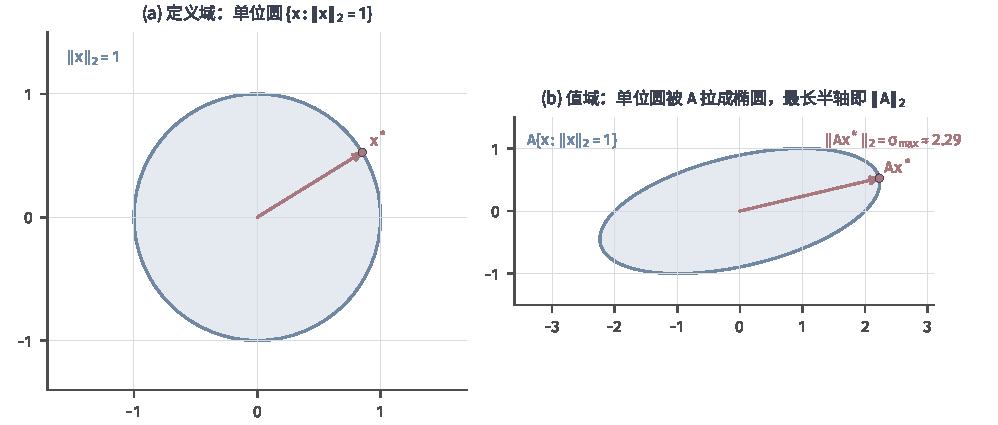
\includegraphics[width=169mm]{figures/00-shared/mathematical-preliminaries-upper/02-linear-spaces/matplotlib/ls-induced-norm-action/ls-induced-norm-action.pdf}
  \caption{诱导矩阵范数衡量最坏放大倍数。左：单位圆$\lVert\bm x\rVert_2=1$；中：同一线性作用$\bm A$把单位圆映成椭圆；右：椭圆上最长的轴给出$\lVert\bm A\rVert_2=\max_{\lVert\bm x\rVert_2=1}\lVert\bm A\bm x\rVert_2$，箭头指示最大放大方向。数值由$\bm A$的教学构造直接得到，是解析例。}
  \label{fig:ls-induced-norm-action}
\end{figure*}


\subsubsection{矩阵范数的性质}

\paragraph{列和与行和公式}
\[
 \begin{gathered}
 \lVert\bm A\rVert_1=\max_j\sum_i|a_{i,j}|,\\
 \lVert\bm A\rVert_\infty=\max_i\sum_j|a_{i,j}|.
 \end{gathered}
\]
第一式按列算：
\[
 \lVert\bm A\bm x\rVert_1=\Bigl\lVert\sum_jx_j\bm A_{:,j}\Bigr\rVert_1\leq\sum_j|x_j|\,\lVert\bm A_{:,j}\rVert_1\leq\Bigl(\max_j\lVert\bm A_{:,j}\rVert_1\Bigr)\lVert\bm x\rVert_1,
\]
而取$\bm x$为最大绝对列和所在列对应的标准坐标向量时等号成立。第二式按行算：对每个$i$，
\[
 |(\bm A\bm x)_i|\leq\sum_j|a_{i,j}|\,|x_j|\leq\Bigl(\sum_j|a_{i,j}|\Bigr)\lVert\bm x\rVert_\infty,
\]
对$i$取最大值即得上界；取输入各坐标为最大绝对行和那一行元素的符号（元素为零处取$1$），等号成立。

\paragraph{谱范数不超过Frobenius范数}
\[
 \begin{gathered}
 \lVert\bm A\bm x\rVert_2\leq\lVert\bm A\rVert_{\mathrm F}\lVert\bm x\rVert_2,\\
 \lVert\bm A\rVert_2\leq\lVert\bm A\rVert_{\mathrm F}.
 \end{gathered}
\]
对每行用$p=q=2$的Hölder不等式，$(\bm A\bm x)_i^2=(\bm A_{i,:}\bm x)^2\leq\lVert\bm A_{i,:}\rVert_2^2\lVert\bm x\rVert_2^2$；对$i$求和，右侧的$\sum_i\lVert\bm A_{i,:}\rVert_2^2$正是$\lVert\bm A\rVert_{\mathrm F}^2$，得到第一式。第一式说明每个比值$\lVert\bm A\bm x\rVert_2/\lVert\bm x\rVert_2$都不超过$\lVert\bm A\rVert_{\mathrm F}$，所以谱范数有限，并得到第二式。

对一般的输入、输出范数，由定理~\ref{thm:ls-norm-equivalence}，存在常数$c_1,c_2>0$，使
\[
 \begin{gathered}
 \lVert\bm y\rVert_\beta\leq c_1\lVert\bm y\rVert_2,\\
 \lVert\bm x\rVert_2\leq c_2\lVert\bm x\rVert_\alpha.
 \end{gathered}
\]
结合刚证明的Frobenius界，得到
\[
 \lVert\bm A\bm x\rVert_\beta
 \leq c_1c_2\lVert\bm A\rVert_{\mathrm F}\lVert\bm x\rVert_\alpha.
\]
所以定义中的上确界有限。

诱导范数满足范数的四条要求：非负性与齐次性由定义直接得到；若$\lVert\bm A\rVert_{\alpha\to\beta}=0$，则每个$\bm A\bm e_j=\bm0$，即$\bm A=\bm0$；三角不等式来自$\lVert(\bm A+\bm B)\bm x\rVert_\beta\leq\lVert\bm A\bm x\rVert_\beta+\lVert\bm B\bm x\rVert_\beta$，两边除以$\lVert\bm x\rVert_\alpha$再取上确界即得。

上确界还在某个方向达到。由齐次性，只需在输入范数单位球面$\{\bm x:\lVert\bm x\rVert_\alpha=1\}$上取上确界。上述下界保证该球面在欧氏坐标中有界，而范数的连续性保证坐标收敛的单位向量列，其极限仍在球面上。取输出范数趋于上确界的单位向量列，逐坐标抽取收敛子列；矩阵乘法和输出范数在坐标下连续，因而子列极限达到上确界。于是定义中的上确界可以写成最大值。

\paragraph{次乘性}
中间范数匹配时，
\[
 \lVert\bm A\bm B\rVert_{\alpha\to\gamma}
 \leq\lVert\bm A\rVert_{\beta\to\gamma}
 \lVert\bm B\rVert_{\alpha\to\beta}.
\]
连续应用两次诱导范数的界：
\[
 \lVert\bm A\bm B\bm x\rVert_\gamma\leq\lVert\bm A\rVert_{\beta\to\gamma}\lVert\bm B\bm x\rVert_\beta\leq\lVert\bm A\rVert_{\beta\to\gamma}\lVert\bm B\rVert_{\alpha\to\beta}\lVert\bm x\rVert_\alpha.
\]
两边除以$\lVert\bm x\rVert_\alpha$再取上确界即得。特别地，反复使用可得$\lVert\bm A^k\rVert_p\leq\lVert\bm A\rVert_p^k$。

\paragraph{Frobenius范数与谱范数的混合界}
\begin{equation}
\begin{gathered}
\lVert\bm A\bm B\rVert_{\mathrm F}
 \leq\lVert\bm A\rVert_2\lVert\bm B\rVert_{\mathrm F}\\
\lVert\bm A\bm B\rVert_{\mathrm F}
 \leq\lVert\bm A\rVert_{\mathrm F}\lVert\bm B\rVert_2.
\end{gathered}
\label{eq:matrix-analysis-mixed-submultiplicativity}
\end{equation}
第一式按列算：
\[
 \lVert\bm A\bm B\rVert_{\mathrm F}^2=\sum_j\lVert\bm A\bm B_{:,j}\rVert_2^2\leq\lVert\bm A\rVert_2^2\sum_j\lVert\bm B_{:,j}\rVert_2^2=\lVert\bm A\rVert_2^2\lVert\bm B\rVert_{\mathrm F}^2.
\]
第二式对转置应用第一式：$\lVert\bm A\bm B\rVert_{\mathrm F}=\lVert\bm B^\top\bm A^\top\rVert_{\mathrm F}\leq\lVert\bm B^\top\rVert_2\lVert\bm A^\top\rVert_{\mathrm F}$，其中转置不改变Frobenius范数，还需要说明$\lVert\bm B^\top\rVert_2=\lVert\bm B\rVert_2$。对固定的$\bm x$，由$p=q=2$的Hölder不等式，$\lVert\bm y\rVert_2=1$时$|\bm y^\top\bm B\bm x|\leq\lVert\bm B\bm x\rVert_2$，而$\bm B\bm x\neq\bm0$时取$\bm y=\bm B\bm x/\lVert\bm B\bm x\rVert_2$即取等号，所以
\[
 \lVert\bm B\rVert_2=\sup_{\lVert\bm x\rVert_2=\lVert\bm y\rVert_2=1}|\bm y^\top\bm B\bm x|.
\]
由于$\bm y^\top\bm B\bm x=\bm x^\top\bm B^\top\bm y$，交换$\bm x,\bm y$的角色，同一个上确界也等于$\lVert\bm B^\top\rVert_2$。结合$\lVert\bm A\rVert_2\leq\lVert\bm A\rVert_{\mathrm F}$，Frobenius范数也满足次乘性：$\lVert\bm A\bm B\rVert_{\mathrm F}\leq\lVert\bm A\rVert_{\mathrm F}\lVert\bm B\rVert_{\mathrm F}$。

\subsection{对偶范数}
\label{sec:ls-dual-norms}

上一章建立了线性泛函；这里已规定向量的大小，便可以进一步问一个读取规则有多“大”。先考虑$V=\mathbb R^d$，并取定该空间上的一种范数。这正是误差分析中的常见问题：误差$\bm r$只知道落在某个范数球内时，一次加权读取$\bm z^\top\bm r$最多变化多少？下面的量就是这个最大值。
\begin{definition}[对偶范数]
\label{def:linear-algebra-dual-norm}
给定$\mathbb R^d$上的范数，相对于标准坐标配对的\term{对偶范数}（dual norm）为
\begin{equation}
 \lVert\bm z\rVert_*=\sup_{\lVert\bm r\rVert\leq1}|\bm z^\top\bm r|.
 \label{eq:linear-algebra-dual-norm-definition}
\end{equation}
\end{definition}
对任意范数，这个上确界有限并可以取到（第~\ref{sec:ls-error-scale-comparison}节）；对$\ell_p$范数，下面还将直接构造取到它的$\bm r$。它满足范数的四条要求，因而是对偶空间上的范数。非负性显然。$\bm z\neq\bm0$时，取$\bm z$的某个非零坐标$z_j$，$\bm r=\bm e_j/\lVert\bm e_j\rVert$给出$|\bm z^\top\bm r|=|z_j|/\lVert\bm e_j\rVert>0$。对每个$\bm r$都有$|(\bm z+\bm w)^\top\bm r|\leq|\bm z^\top\bm r|+|\bm w^\top\bm r|$，取上确界即得三角不等式；齐次性由$|(c\bm z)^\top\bm r|=|c|\,|\bm z^\top\bm r|$得到。图~\ref{fig:ls-dual-norm-unit-ball}把这个最大值画成支撑线最后接触单位球的位置。

\begin{figure}[!htb]
  \centering
  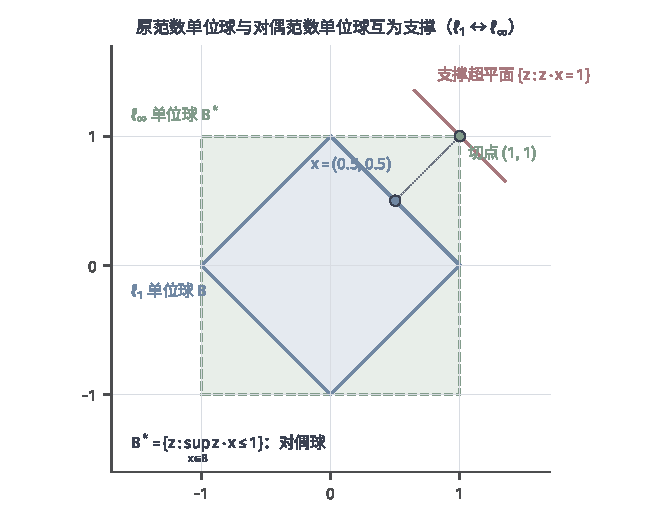
\includegraphics[width=112mm]{figures/00-shared/mathematical-preliminaries-upper/02-linear-spaces/matplotlib/ls-dual-norm-unit-ball/ls-dual-norm-unit-ball.pdf}
  \caption{对偶范数的几何：在原范数单位球$\lVert\bm r\rVert\leq1$上求线性读取$\bm z^\top\bm r$的最大值。左：原单位球（灰色）与读取方向$\bm z$；右：支撑直线最后接触单位球处给出$\lVert\bm z\rVert_*=\max_{\lVert\bm r\rVert\leq1}|\bm z^\top\bm r|$。对偶单位球（虚线）与原单位球互为极体，为解析教学例。}
  \label{fig:ls-dual-norm-unit-ball}
\end{figure}

对$\ell_p$范数，
\begin{equation}
\begin{gathered}
(\lVert\cdot\rVert_p)_*=\lVert\cdot\rVert_q\\
\frac1p+\frac1q=1,
\end{gathered}
\label{eq:linear-algebra-lp-duality}
\end{equation}
并且由齐次性，对$\rho\geq0$有
\begin{equation}
 \max_{\lVert\bm r\rVert_p\leq\rho}|\bm z^\top\bm r|
 =\rho\lVert\bm z\rVert_q.
 \label{eq:linear-algebra-linear-perturbation-duality}
\end{equation}
本节的Hölder不等式（定理~\ref{thm:linear-algebra-holder}）给出$\ell_p$单位球上的上界$\lVert\bm z\rVert_q$。这个上界可以达到：$1<p<\infty$且$\bm z\neq\bm0$时取$r_j=|z_j|^{q-1}\operatorname{sgn}(z_j)/\lVert\bm z\rVert_q^{q-1}$；$\bm z=\bm0$时上界为零，任取可行输入即可。$p=1$时把单位预算全部放在$|z_j|$最大的坐标上；$p=\infty$时逐坐标取$r_j=\operatorname{sgn}(z_j)$。下面固定一个读取，比较三种误差预算。
\begin{example}[同一读取在三种误差预算下的最大变化]
\label{ex:ls-dual-norm-three-budgets}
给定：读取方向$\bm z=(2,-1)^\top$，即读取$\bm z^\top\bm r=2r_1-r_2$。

计算：在$\ell_1$单位球上，把单位预算全部放在$|z_j|$最大的第一个坐标，$\bm r=(1,0)^\top$给出最大值$\lVert\bm z\rVert_\infty=2$。在$\ell_2$单位球上，取$\bm r=\bm z/\lVert\bm z\rVert_2=(2,-1)^\top/\sqrt5$，最大值为$\lVert\bm z\rVert_2=\sqrt5$。在$\ell_\infty$单位球上，逐坐标取$r_j=\operatorname{sgn}(z_j)$，$\bm r=(1,-1)^\top$给出最大值$\lVert\bm z\rVert_1=3$。若误差预算为$|r_j|\leq0.01$，在式~\eqref{eq:linear-algebra-linear-perturbation-duality}中取$p=\infty$、$\rho=0.01$，最大变化为$0.01\cdot(2+1)=0.03$，由$\bm r=(0.01,-0.01)^\top$达到。

结论：同一次读取在$\ell_1$、$\ell_2$、$\ell_\infty$单位球上的最大值依次为$2$、$\sqrt5$、$3$；改变误差预算的形状，最坏方向和最大变化都随之改变。
\end{example}
图~\ref{fig:linear-algebra-dual-unit-balls}画出这三种情形下的最坏方向。
\begin{figure*}[htbp]
  \centering
  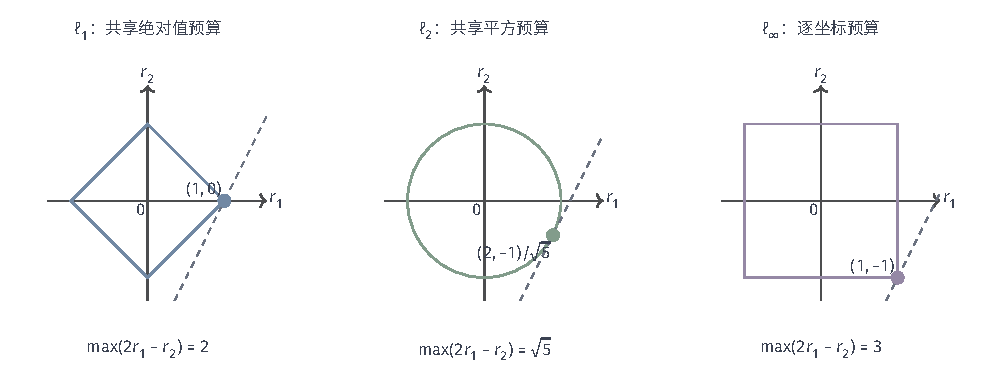
\includegraphics[width=168.998mm]{figures/00-shared/mathematical-preliminaries-upper/02-linear-spaces/tikz/linear-algebra-dual-unit-balls/figure.pdf}
  \caption{同一线性读取$2r_1-r_2$在$\ell_1$、$\ell_2$、$\ell_\infty$单位球上的最大值依次为$2$、$\sqrt5$、$3$。虚线为最后接触可行集的支撑直线，点为最大化方向。三图坐标尺度相同，均为解析教学例；改变允许误差的形状会改变误差常数。}
  \label{fig:linear-algebra-dual-unit-balls}
\end{figure*}

误差预算按$\ell_\infty$给出时，读取方向要按$\ell_1$计量；预算按$\ell_2$给出时，读取方向仍按$\ell_2$计量。所以讨论“输入误差最多引起多大输出误差”时，必须先说清误差用哪种范数度量。

\subsection{商范数}
\label{sec:ls-quotient-norms}

有限维子空间的闭性还可以用来为商空间定义范数。第~\ref{sec:ls-quotient-spaces}节的商空间$V/U$把相差$U$中向量的点看成同一个类$\bm x+U$，那里只建立了线性结构。同一类中各点到$U$的距离相同：若$\bm x'=\bm x+\bm u_0$，$\bm u_0\in U$，则$\bm u$遍历$U$时$\bm u-\bm u_0$也遍历$U$，所以$d(\bm x',U)=d(\bm x,U)$。因此可以把这个距离当作类的大小，称为商范数
\[
 \lVert\bm x+U\rVert_{V/U}=d(\bm x,U)=\inf_{\bm u\in U}\lVert\bm x-\bm u\rVert .
\]
它满足范数的三条要求。三角不等式：对任意$\bm u,\bm u'\in U$，$d(\bm x+\bm y,U)\leq\lVert(\bm x-\bm u)+(\bm y-\bm u')\rVert\leq\lVert\bm x-\bm u\rVert+\lVert\bm y-\bm u'\rVert$，再对$\bm u,\bm u'$分别取下确界。齐次性：$c\neq0$时$cU=U$，所以$d(c\bm x,U)=|c|\,d(\bm x,U)$；$c=0$时两边都为零。正定性要求$d(\bm x,U)=0$只在$\bm x+U=U$即$\bm x\in U$时发生，这正是上面的闭性结论。

\paragraph{一般范数下的最近点}
距离$d(\bm y,U)$定义为下确界，它总能取到吗？由$d(\bm y,U)\leq\lVert\bm y-\bm0\rVert=\lVert\bm y\rVert$，而$\lVert\bm u\rVert>2\lVert\bm y\rVert$时$\lVert\bm y-\bm u\rVert\geq\lVert\bm u\rVert-\lVert\bm y\rVert>\lVert\bm y\rVert$，所以只需在$K=\{\bm u\in U:\lVert\bm u\rVert\leq2\lVert\bm y\rVert\}$上找最小值。由子空间闭性，$K$是闭有界集，按“收敛与连续性”一段的最值论证，连续函数$\bm u\mapsto\lVert\bm y-\bm u\rVert$在其上取到最小值，所以最近点存在。

唯一性却可能失败。
\begin{example}[反例：$\ell_\infty$范数下最近点不唯一]
\label{ex:ls-linf-nonunique-nearest}
给定：$\mathbb R^2$取$\ell_\infty$范数，子空间$U=\operatorname{span}\{(1,0)^\top\}$，点$\bm y=(0,1)^\top$。

计算：$U$中的点写成$(t,0)^\top$，
\[
 \lVert\bm y-(t,0)^\top\rVert_\infty=\max\{|t|,1\}\geq1,
\]
等号当且仅当$|t|\leq1$时成立。

结论：$d(\bm y,U)=1$，所有满足$|t|\leq1$的点$(t,0)^\top$都是最近点，最近点不唯一。
\end{example}
内积诱导的范数下最近点唯一，并由正规方程算出（第~\ref{sec:ls-subspace-nearest-points}节）。

% 第5章第6节：内积空间（内积与内积空间、Gram矩阵、子空间之间的正交、标准正交基的定义和性质、标准正交基的构建、伴随、完备性与Hilbert空间）。

\section{内积空间与Gram矩阵}
\label{sec:ls-inner-product-spaces}

上一节用范数度量大小，但范数不给出角度：一般范数下谈不上两个方向是否垂直，向子空间的最近点也可能不唯一（示例~\ref{ex:ls-linf-nonunique-nearest}）。第~\ref{chap:linear-operations}章在$\mathbb R^d$上定义了欧氏内积，用逐项相乘再求和完成具体计算。本节提取这种计算的共同规则，在一般线性空间上定义内积。

本节先从内积公理建立长度、夹角与基本不等式，再用Gram矩阵记录一组向量之间的配对。随后两节讨论正交投影、标准正交基、泛函表示与伴随；这些工具主要在有限维空间中构造。

\subsection{内积与内积诱导的范数}
\label{sec:ls-inner-product-definition}

本小节只用内积的公理推出长度、夹角及相关不等式，说明内积空间都是赋范空间，并指出并非每个范数都来自内积。

\paragraph{一般线性空间上的内积}
欧氏内积对每个变量都保持线性组合，交换两个变量不改变结果，向量与自身的配对只在零向量处为零。这些性质只涉及线性运算，因此可以用来定义一般空间上的内积。
\begin{definition}[内积空间]
\label{def:functional-inner-product-space}
\label{def:linear-algebra-inner-product}
设$V$是实线性空间。映射$\langle\cdot,\cdot\rangle:V\times V\to\mathbb R$若对任意$\bm x,\bm y,\bm z\in V$与$a,b\in\mathbb R$满足
\begin{enumerate}
 \item 双线性：$\langle a\bm x+b\bm y,\bm z\rangle=a\langle\bm x,\bm z\rangle+b\langle\bm y,\bm z\rangle$，且$\langle\bm z,a\bm x+b\bm y\rangle=a\langle\bm z,\bm x\rangle+b\langle\bm z,\bm y\rangle$；
 \item 对称性：$\langle\bm x,\bm y\rangle=\langle\bm y,\bm x\rangle$；
 \item 正定性：$\langle\bm x,\bm x\rangle\geq0$，且$\langle\bm x,\bm x\rangle=0$当且仅当$\bm x=\bm0$，
\end{enumerate}
就称为$V$上的\term{内积}（inner product）；配备内积的线性空间$(V,\langle\cdot,\cdot\rangle)$称为\term{内积空间}（inner-product space）。
\end{definition}
\paragraph{欧氏内积的公理检验}

下面逐条验证欧氏内积满足定义~\ref{def:linear-algebra-inner-product}的三条公理。

设$\bm x,\bm y,\bm z\in\mathbb R^d$，$a,b\in\mathbb R$。

先看对称性。
\[
 \langle\bm x,\bm y\rangle=\langle\bm y,\bm x\rangle,
\]
因为每一项$x_jy_j=y_jx_j$。

再看双线性。
\[
 \langle a\bm x+b\bm z,\bm y\rangle=a\langle\bm x,\bm y\rangle+b\langle\bm z,\bm y\rangle,
\]
由有限和的运算法则$\sum_j(ax_j+bz_j)y_j=a\sum_jx_jy_j+b\sum_jz_jy_j$得到；再由对称性，对第二个变量同样成立。

最后看正定性。
\[
 \begin{gathered}
 \langle\bm x,\bm x\rangle\geq0,\\
 \langle\bm x,\bm x\rangle=0\iff\bm x=\bm0,
 \end{gathered}
\]
因为$\langle\bm x,\bm x\rangle=\sum_jx_j^2$，而非负数之和为零时每一项都为零。


Frobenius内积满足定义~\ref{def:linear-algebra-inner-product}的三条公理：它对两个变量分别线性；交换两个矩阵不改变各项乘积，因而对称；$\langle\bm A,\bm A\rangle_{\mathrm F}=\sum_{i,j}a_{i,j}^2$非负，并且只在$\bm A=\bm0$时为零。这正是把$mn$个元素看作坐标时欧氏内积的三条性质，所以它确实是同形矩阵上的一个内积，下面从公理推出的一般结论对它同样成立。

标准内积之外，一般空间上可以有各种内积。下面在$P_1$上规定一个只看两点取值的内积，后面的算例会反复用到它。
\begin{example}[只看两点取值的内积]
\label{ex:ls-two-point-inner-product}
给定：$P_1$上的规则$\langle f,g\rangle=f(0)g(0)+f(1)g(1)$。

验证：右端对$f$与对$g$分别是线性的，交换$f,g$也不改变右端，所以双线性与对称性成立。$\langle f,f\rangle=f(0)^2+f(1)^2\geq0$；若它为零，则$f(0)=f(1)=0$，对$f=a+bt$即$a=0$、$a+b=0$，故$f=0$，正定性也成立。

结论：这一规则是$P_1$上的内积。它只看函数在$t=0,1$两点的取值，与系数向量$(a,b)^\top$的欧氏内积不同：例如$\langle1,t\rangle=1\cdot0+1\cdot1=1$，而$1$与$t$的系数向量$(1,0)^\top$、$(0,1)^\top$的欧氏内积为零。
\end{example}

\paragraph{长度与勾股定理}
与$\mathbb R^d$中一样，内积给出长度$\lVert\bm v\rVert=\sqrt{\langle\bm v,\bm v\rangle}$；$\langle\bm x,\bm y\rangle=0$时称$\bm x,\bm y$正交。正交的两个向量满足勾股定理：展开$\lVert\bm x+\bm y\rVert^2=\lVert\bm x\rVert^2+2\langle\bm x,\bm y\rangle+\lVert\bm y\rVert^2$，交叉项为零，得$\lVert\bm x+\bm y\rVert^2=\lVert\bm x\rVert^2+\lVert\bm y\rVert^2$。

\paragraph{Cauchy--Schwarz不等式}
平面上两个非零向量的夹角$\theta$满足
\[
 \langle\bm x,\bm y\rangle=\lVert\bm x\rVert\,\lVert\bm y\rVert\cos\theta.
\]
要在一般内积空间中反过来用这个关系定义夹角，须先保证内积除以两个长度之积以后总落在$[-1,1]$中。
\begin{theorem}[Cauchy--Schwarz不等式]
\label{thm:linear-algebra-cauchy-schwarz}
对任一内积及其长度，任意向量$\bm x,\bm y$满足
\begin{equation}
 |\langle\bm x,\bm y\rangle|\leq\lVert\bm x\rVert\,\lVert\bm y\rVert,
 \label{eq:prelim-cauchy-schwarz}
\end{equation}
等号成立当且仅当其中一个向量是另一个向量的实数倍。
\end{theorem}
\begin{proof}
$\bm y=\bm0$时两边都为零。否则对任意实数$s$，向量$\bm x-s\bm y$的长度平方非负；按内积的对称性与双线性展开，
\[
 0\leq\lVert\bm x-s\bm y\rVert^2
 =\lVert\bm x\rVert^2-2s\langle\bm x,\bm y\rangle+s^2\lVert\bm y\rVert^2.
\]
右侧是$s$的二次函数，二次项系数为正，取顶点$s=\langle\bm x,\bm y\rangle/\lVert\bm y\rVert^2$时最小，此时右侧化为$\lVert\bm x\rVert^2-\langle\bm x,\bm y\rangle^2/\lVert\bm y\rVert^2$。它非负，两边乘以$\lVert\bm y\rVert^2$再开平方，即得不等式。$\bm y\neq\bm0$时，等号成立当且仅当对这个$s$有$\bm x-s\bm y=\bm0$，即$\bm x$是$\bm y$的实数倍；连同$\bm y=\bm0$的情形即得等号条件。
\end{proof}
证明只用了内积的三条公理，所以不等式对每一种内积都成立。在$\mathbb R^d$的标准内积下，它就是$p=q=2$的Hölder不等式（定理~\ref{thm:linear-algebra-holder}）；对Frobenius内积，它给出$|\langle\bm A,\bm B\rangle_{\mathrm F}|\leq\lVert\bm A\rVert_{\mathrm F}\lVert\bm B\rVert_{\mathrm F}$。

\paragraph{三角不等式}
内积给出的长度是否满足定义~\ref{def:ls-normed-space}中范数的三条要求？正定性直接来自内积的正定性，齐次性来自$\langle c\bm x,c\bm x\rangle=c^2\langle\bm x,\bm x\rangle$；需要证明的是三角不等式，Cauchy--Schwarz不等式正好控制展开式中的交叉项。
\begin{theorem}[内积诱导长度的三角不等式]
\label{thm:ls-inner-product-triangle}
设$V$是内积空间，$\lVert\bm v\rVert=\sqrt{\langle\bm v,\bm v\rangle}$，则对任意$\bm x,\bm y\in V$，
\[
 \lVert\bm x+\bm y\rVert\leq\lVert\bm x\rVert+\lVert\bm y\rVert,
\]
等号成立当且仅当其中一个向量是另一个向量的非负实数倍。
\end{theorem}
\begin{proof}
按双线性与对称性展开平方，再对交叉项用$\langle\bm x,\bm y\rangle\leq|\langle\bm x,\bm y\rangle|$与Cauchy--Schwarz不等式~\eqref{eq:prelim-cauchy-schwarz}：
\[
 \begin{aligned}
 \lVert\bm x+\bm y\rVert^2
 &=\lVert\bm x\rVert^2+2\langle\bm x,\bm y\rangle+\lVert\bm y\rVert^2\\
 &\leq\lVert\bm x\rVert^2+2\lVert\bm x\rVert\lVert\bm y\rVert+\lVert\bm y\rVert^2\\
 &=(\lVert\bm x\rVert+\lVert\bm y\rVert)^2.
 \end{aligned}
\]
两边都非负，开平方即得不等式。等号成立当且仅当$\langle\bm x,\bm y\rangle=\lVert\bm x\rVert\,\lVert\bm y\rVert$。若$\bm y=\bm0$，结论显然；若$\bm y\neq\bm0$，由Cauchy--Schwarz不等式的等号条件，$\bm x=s\bm y$，代入得$s\lVert\bm y\rVert^2=|s|\,\lVert\bm y\rVert^2$，即$s\geq0$。反过来，$\bm x=s\bm y$且$s\geq0$时两侧都等于$(1+s)\lVert\bm y\rVert$。
\end{proof}
于是内积给出的长度满足范数的三条要求，每个内积空间都是赋范空间，第~\ref{sec:ls-normed-spaces}节关于收敛与完备性的讨论都适用于它。

\paragraph{平行四边形恒等式}
欧氏范数由内积给出，还满足\term{平行四边形恒等式}。一般范数未必满足这条等式。几何上，它表示平行四边形两条对角线长度的平方和等于四条边长度的平方和。
\begin{theorem}[平行四边形恒等式]
\label{thm:linear-algebra-parallelogram}
设$V$是实内积空间，$\bm x,\bm y\in V$，以该内积诱导的范数计量长度，则
\begin{equation}
 \lVert\bm x+\bm y\rVert^2+\lVert\bm x-\bm y\rVert^2
 =2\lVert\bm x\rVert^2+2\lVert\bm y\rVert^2.
 \label{eq:functional-parallelogram-identity}
\end{equation}
欧氏范数是这一结论的特例。
\end{theorem}
\begin{proof}
记$\lVert\bm u\rVert^2=\langle\bm u,\bm u\rangle$。由内积的双线性和对称性，分别展开和向量与差向量的长度平方：
\[
 \begin{aligned}
 \lVert\bm x+\bm y\rVert^2
 &=\lVert\bm x\rVert^2+2\langle\bm x,\bm y\rangle+\lVert\bm y\rVert^2,\\
 \lVert\bm x-\bm y\rVert^2
 &=\lVert\bm x\rVert^2-2\langle\bm x,\bm y\rangle+\lVert\bm y\rVert^2.
 \end{aligned}
\]
两式相加，交叉项相互抵消，得到所需恒等式。证明只用了内积公理，因此既适用于欧氏内积，也适用于定义~\ref{def:linear-algebra-inner-product}中的任一实内积。
\end{proof}

反过来，恒等式可以检验一个范数是否来自内积：只要某个范数在一对向量上使恒等式两侧不等，它就不可能由任何内积给出。下面的反例用这个办法检验$\ell_1$与$\ell_\infty$范数。
\begin{example}[反例：$\ell_1$与$\ell_\infty$范数不来自内积]
\label{ex:ls-l1-linf-not-inner-product}
给定：$\mathbb R^2$中的$\bm x=\bm e_1$、$\bm y=\bm e_2$，于是$\bm x+\bm y=(1,1)^\top$，$\bm x-\bm y=(1,-1)^\top$。
计算：对$\ell_1$范数，
\[
 \begin{gathered}
 \lVert\bm x+\bm y\rVert_1^2+\lVert\bm x-\bm y\rVert_1^2=2^2+2^2=8,\\
 2\lVert\bm x\rVert_1^2+2\lVert\bm y\rVert_1^2=2\cdot1^2+2\cdot1^2=4;
 \end{gathered}
\]
对$\ell_\infty$范数，
\[
 \begin{gathered}
 \lVert\bm x+\bm y\rVert_\infty^2+\lVert\bm x-\bm y\rVert_\infty^2=1^2+1^2=2,\\
 2\lVert\bm x\rVert_\infty^2+2\lVert\bm y\rVert_\infty^2=4.
 \end{gathered}
\]
结论：两种范数都使恒等式两侧不等。所以不存在内积使$\lVert\bm x\rVert_1=\sqrt{\langle\bm x,\bm x\rangle}$对一切$\bm x$成立，$\ell_\infty$范数同样不是由内积给出的长度。
\end{example}

内积还可由它诱导的范数恢复。在实空间中，分别展开两个平方并相减，得到极化恒等式
\[
 \langle x,y\rangle=\frac14\bigl(\|x+y\|^2-\|x-y\|^2\bigr).
\]
因此两个实内积若给出同一个范数，就必相同。这也说明平行四边形恒等式不是任意范数的自动性质，而是内积几何对长度的约束。

\paragraph{夹角}
由Cauchy--Schwarz不等式，非零向量的夹角$\theta\in[0,\pi]$可以由
\[
 \cos\theta=\frac{\langle\bm x,\bm y\rangle}{\lVert\bm x\rVert\,\lVert\bm y\rVert}
 =\left\langle\frac{\bm x}{\lVert\bm x\rVert},\frac{\bm y}{\lVert\bm y\rVert}\right\rangle
\]
定义。第二种写法说明，夹角只比较方向：先把两个向量各自归一化为单位向量，再取内积；$\bm x$与$c\bm x$（$c>0$）给出同一个方向。正交恰好对应$\theta=\pi/2$，这就是把正交称为垂直的理由；等号条件说明$\cos\theta=\pm1$恰好对应两个向量共线。夹角要求长度来自同一个内积，一边用$\ell_2$、一边用$\ell_1$计量长度时，比值没有几何意义。

回到第~\ref{chap:linear-operations}章两个特征的取值向量，看它们的夹角。
\begin{example}[贯穿例两列的夹角]
\label{ex:ls-nearly-collinear-angle}
给定：$\bm c_1=(1,1,1)^\top$与$\bm c_2=(1,1+\varepsilon,1-\varepsilon)^\top$，取欧氏内积。

计算：$\langle\bm c_1,\bm c_2\rangle=1+(1+\varepsilon)+(1-\varepsilon)=3$，$\lVert\bm c_1\rVert_2^2=3$，$\lVert\bm c_2\rVert_2^2=1+(1+\varepsilon)^2+(1-\varepsilon)^2=3+2\varepsilon^2$，所以
\begin{equation}
 \cos\theta_\varepsilon=\frac{3}{\sqrt3\,\sqrt{3+2\varepsilon^2}}
 =\frac{1}{\sqrt{1+2\varepsilon^2/3}}\longrightarrow1\qquad(\varepsilon\to0).
 \label{eq:linear-algebra-nearly-collinear-angle}
\end{equation}
$\varepsilon=0.1$时$\cos\theta_\varepsilon\approx0.9967$，夹角约$4.7^\circ$；$\varepsilon=0.01$时$\cos\theta_\varepsilon\approx0.99997$，夹角不到$0.5^\circ$。

结论：$\varepsilon\to0$时两列的夹角趋于零；当$\varepsilon$非零且很小时，两个向量不重合，却几乎同向。
\end{example}
两个向量不重合却几乎同向，称为\term{近共线}（nearly collinear）。“近”指作为$\mathbb R^3$中向量的两列夹角很小，不是说各个样本点彼此接近。夹角也依赖所用的内积，换一种内积，同两个向量的夹角会改变。

平行四边形恒等式及其后的反例已经说明，并非每个范数都来自内积。因此，一般范数只能度量大小，不能直接使用这里的公式定义夹角。

\paragraph{复内积的约定}
前面的定义和夹角讨论都针对实空间。复空间中，若两个槽位都按复数线性且满足实数式的对称性，那么$\langle\mathrm i\bm x,\mathrm i\bm x\rangle=-\langle\bm x,\bm x\rangle$，无法对非零向量保持正定。因此复内积采用不同约定：对第一个变量共轭线性，对第二个变量线性，并满足$\langle\bm x,\bm y\rangle=\overline{\langle\bm y,\bm x\rangle}$。标准例子是$\langle\bm x,\bm y\rangle=\bm x^*\bm y$，其中$\bm x^*$表示共轭转置；仍要求$\langle\bm x,\bm x\rangle>0$对非零$\bm x$成立。

复内积同样满足Cauchy--Schwarz不等式。若$\bm y\ne\bm0$，在$\|\bm x-\alpha\bm y\|^2\geq0$中取$\alpha=\langle\bm y,\bm x\rangle/\|\bm y\|^2$，展开可得$|\langle\bm x,\bm y\rangle|^2\leq\|\bm x\|^2\|\bm y\|^2$。因此平方根仍给出范数；但复内积可能不是实数，实空间用余弦定义夹角的公式不能直接照搬。下面的具体证明继续使用实内积，复情形需要把转置相应改为共轭转置。

\paragraph{有限维完备性与Hilbert空间}
\label{sec:ls-hilbert-spaces}
内积诱导的范数使内积空间成为赋范空间。若这个范数下的每个柯西列都收敛到空间内的元素，就称它为\term{Hilbert空间}（Hilbert space，也译作希尔伯特空间）。由定理~\ref{thm:ls-finite-dimensional-complete}，有限维内积空间都满足这一条件。

这里的完备性来自有限个坐标和标量完备性，不能直接推广到无限维。无限正交级数、闭子空间上的投影以及连续泛函的表示，都需要另行核对收敛、闭性和连续性；这些结论在\BookChapterRef{chap:functional-analysis-and-approximation}{第~\ref{chap:functional-analysis-and-approximation}章}建立。

\subsection{Gram矩阵}
\label{sec:ls-gram-psd}

加权内积由一个正定矩阵给出。反过来看，一组向量的全部两两内积也排成一个对称矩阵。本小节说明，这样的矩阵恰好是全部半正定矩阵，从中可以读出这组向量是否线性无关、是否两两正交；最后用基的Gram矩阵写出一般内积空间在坐标下的计算公式。

\paragraph{正定矩阵与半正定矩阵}
$n$阶对称矩阵$\bm M$与向量$\bm x\in\mathbb R^n$给出一个数
\[
 q(\bm x)=\sum_{i=1}^n\sum_{j=1}^n m_{i,j}x_ix_j,
\]
称为$\bm M$的二次型；用矩阵乘法，它写作$\bm x^\top\bm M\bm x$。

若对每个非零$\bm x$都有$q(\bm x)>0$，就称$\bm M$\term{正定}（positive definite），记作$\bm M\succ\bm0$；若只保证$q(\bm x)\geq0$对一切$\bm x$成立，就称$\bm M$\term{半正定}（positive semidefinite），记作$\bm M\succeq\bm0$。对两个同阶对称矩阵，$\bm M\succeq\bm N$表示$\bm M-\bm N\succeq\bm0$，即$\bm M$的二次型处处不小于$\bm N$的二次型；它比较的是两个二次型，不是逐个元素。

判断正定性，要看二次型能否在某个非零向量处取到零或负值。下面用配方比较两个二阶矩阵。
\begin{example}[用配方区分正定与半正定]
\label{ex:ls-pd-psd-completing-square}
给定：$\bm M=\left[\begin{smallmatrix}4&2\\2&2\end{smallmatrix}\right]$，$\bm N=\left[\begin{smallmatrix}1&1\\1&1\end{smallmatrix}\right]$。
计算：两者的二次型配方为
\[
 \begin{aligned}
 q_{\bm M}(\bm x)&=4x_1^2+4x_1x_2+2x_2^2=(2x_1+x_2)^2+x_2^2,\\
 q_{\bm N}(\bm x)&=x_1^2+2x_1x_2+x_2^2=(x_1+x_2)^2.
 \end{aligned}
\]
$q_{\bm M}$是两个平方之和，只在$2x_1+x_2=0$且$x_2=0$，即$\bm x=\bm0$时为零。$q_{\bm N}$处处非负，但在非零向量$\bm x=(1,-1)^\top$处为零。
结论：$\bm M\succ\bm0$；$\bm N\succeq\bm0$，但$\bm N$不是正定矩阵。
\end{example}

对角矩阵的二次型是$\sum_id_ix_i^2$。若全部$d_i>0$，每个非零$\bm x$都使它为正；若某个$d_i\leq0$，取$\bm x=\bm e_i$就得到$q(\bm e_i)=d_i\leq0$。所以对角矩阵正定当且仅当全部$d_i>0$，例如$\bm I_n\succ\bm0$。

正定性要对全部非零向量检查，只看元素的符号并不够，下面的反例说明这一点。
\begin{example}[反例：元素全为正的对称矩阵未必正定]
\label{ex:ls-positive-entries-not-pd}
给定：$\bm M=\left[\begin{smallmatrix}1&2\\2&1\end{smallmatrix}\right]$，四个元素都为正。
计算：它的二次型为$q(\bm x)=x_1^2+4x_1x_2+x_2^2$。取$\bm x=(1,-1)^\top$，
\[
 q(\bm x)=1^2+4\cdot1\cdot(-1)+(-1)^2=-2.
\]
结论：$q(\bm x)<0$，所以$\bm M$不是正定矩阵，也不是半正定矩阵。
\end{example}


\paragraph{Gram矩阵}
\phantomsection
\label{sec:ls-gram-orthogonality}
正交是两个向量之间的关系。一组向量$\bm b_1,\ldots,\bm b_r$之间有$r^2$个配对值，怎样一次记录它们，并从中读出这组向量是否两两正交、某个线性组合会不会退化为零？
\begin{definition}[有限向量族的Gram矩阵]
\label{def:linear-algebra-gram-matrix}
设$\bm b_1,\ldots,\bm b_r$是内积空间$V$中的向量。以$g_{i,j}=\langle\bm b_i,\bm b_j\rangle$为元素的$r$阶矩阵$\bm G$称为它们的\term{Gram矩阵}（Gram matrix）。在$\mathbb R^m$中，若$\bm B$以这些向量为列，则欧氏内积下$\bm G=\bm B^\top\bm B$，加权内积$\langle\cdot,\cdot\rangle_{\bm M}$下$\bm G=\bm B^\top\bm M\bm B$。
\end{definition}
矩阵形式来自乘积的元素公式：$(\bm B^\top\bm B)_{i,j}$是$\bm B^\top$的第$i$行（即$\bm b_i^\top$）与$\bm B$的第$j$列相乘。由内积的对称性，$\bm G$是对称矩阵。

对任意系数向量$\bm a\in\mathbb R^r$，按双线性展开得
\[
 \bm a^\top\bm G\bm a=\sum_{i,j}a_ia_j\langle\bm b_i,\bm b_j\rangle=\Bigl\lVert\sum_j a_j\bm b_j\Bigr\rVert^2\geq0,
\]
所以Gram矩阵半正定。它正定，当且仅当只有全零系数使线性组合$\sum_ja_j\bm b_j$为零，即这组向量线性无关（第~\ref{sec:ls-linear-dependence}节）：组合为零时平方长度为零，组合非零时平方长度为正。

正定的Gram矩阵可逆：若$\bm G\bm a=\bm0$，则$\bm a^\top\bm G\bm a=0$，从而$\bm a=\bm0$，零空间为零（第~\ref{sec:ls-injective-surjective-invertible}节）。正交性也写在Gram矩阵里：$\bm G$是对角矩阵恰好表示这组向量两两正交，$\bm G=\bm I_r$则表示它们两两正交且长度都为$1$。图~\ref{fig:ls-gram-matrix-coefficients}把两条向量的两两内积排成数表。
\begin{figure}[!htb]
  \centering
  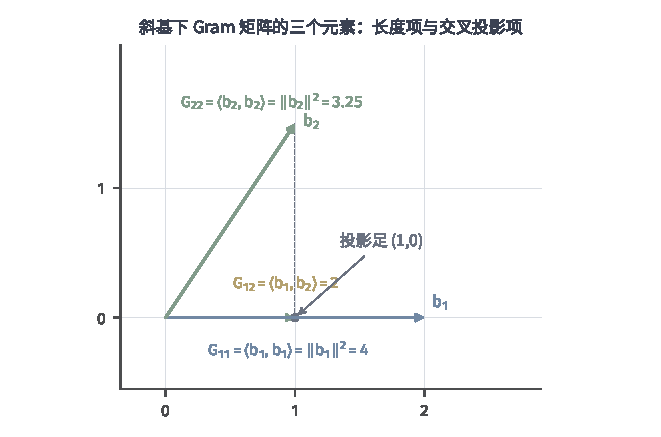
\includegraphics[width=112mm]{figures/00-shared/mathematical-preliminaries-upper/02-linear-spaces/matplotlib/ls-gram-matrix-coefficients/ls-gram-matrix-coefficients.pdf}
  \caption{Gram矩阵把一组基向量的两两内积排成数表。左：平面上两条不垂直的基向量$\bm b_1,\bm b_2$及其夹角；右：$G_{i,j}=\langle\bm b_i,\bm b_j\rangle$构成的$2\times2$Gram矩阵，对角元为各向量长度平方，非对角元为夹角投影。基越接近正交，非对角元越接近零；两向量共线时，某个非零组合的平方长度为零，Gram矩阵不再正定。向量与矩阵均为解析教学例。}
  \label{fig:ls-gram-matrix-coefficients}
\end{figure}

近共线在Gram矩阵上怎样表现？
\begin{example}[近共线两列的Gram矩阵]
\label{ex:ls-nearly-collinear-gram}
给定：贯穿例的两列$\bm c_1,\bm c_2$，取欧氏内积。

计算：由示例~\ref{ex:ls-nearly-collinear-angle}中的三个内积，
\[
\begin{gathered}
\bm G=\bm X_\varepsilon^\top\bm X_\varepsilon=\begin{bmatrix}3&3\\3&3+2\varepsilon^2\end{bmatrix}\\
\bm a^\top\bm G\bm a=3(a_1+a_2)^2+2\varepsilon^2a_2^2 .
\end{gathered}
\]
$\varepsilon\neq0$时，二次型只在$a_1=a_2=0$时为零，所以$\bm G$正定。取$\bm a=(1,-1)^\top$，二次型只有$2\varepsilon^2$；对应的组合$\bm c_1-\bm c_2=-\varepsilon\bm q$确实很短。

结论：$\bm G$正定，与两列线性无关一致；但存在系数使二次型接近零。近共线在Gram矩阵上表现为“正定但几乎退化”。
\end{example}

\paragraph{Gram因子定理}
Gram矩阵总是半正定的。反过来，每个半正定矩阵是否都是某组向量的Gram矩阵？关键是把半正定矩阵写成欧氏平方和，这一分解也说明加权配对不必当作新的几何。
\begin{theorem}[半正定矩阵的配方因子]
\label{thm:ls-gram-factor}
设$\bm M\in\mathbb R^{r\times r}$对称半正定，则存在$\bm L\in\mathbb R^{r\times r}$使$\bm M=\bm L^\top\bm L$；若$\bm M$正定，可取$\bm L$可逆。
\end{theorem}
\begin{proof}
对$r$归纳。$r=1$时$\bm M=(m_{1,1})$且$m_{1,1}\geq0$，取$\bm L=(\sqrt{m_{1,1}})$即可。

设$r>1$。若所有对角元都为零，任取$i\neq j$，把$\bm x=\bm e_i+t\bm e_j$代入半正定性：
\[
 0\leq\bm x^\top\bm M\bm x=m_{i,i}+2t\,m_{i,j}+t^2m_{j,j}=2t\,m_{i,j},
\]
对正负$t$同时成立迫使$m_{i,j}=0$，于是$\bm M=\bm0$，取$\bm L=\bm0$。

否则存在正的对角元。取一个置换矩阵$\bm P$把它换到首位（行列同步交换）；$\bm P$的各列是互不相同的标准坐标向量，所以$\bm P^\top\bm P=\bm P\bm P^\top=\bm I$。记
\[
\begin{gathered}
\widetilde{\bm M}=\bm P\bm M\bm P^\top
 =\begin{bmatrix}a&\bm b^\top\\ \bm b&\bm C\end{bmatrix}\\
a>0.
\end{gathered}
\]
$\widetilde{\bm M}$仍对称半正定，因为$\bm x^\top\widetilde{\bm M}\bm x=(\bm P^\top\bm x)^\top\bm M(\bm P^\top\bm x)\geq0$。对第一个变量配方：令$\bm x=(-\bm b^\top\bm u/a,\bm u)$，展开得$\bm x^\top\widetilde{\bm M}\bm x=\bm u^\top(\bm C-\bm b\bm b^\top/a)\bm u\geq0$，故余项$\bm M'=\bm C-\bm b\bm b^\top/a$仍半正定。由归纳假设$\bm M'=\bm L'^\top\bm L'$，取上三角因子
\[
 \widetilde{\bm L}=\begin{bmatrix}\sqrt a&\bm b^\top/\sqrt a\\ \bm0&\bm L'\end{bmatrix},
\]
按分块乘法直接相乘得
\[
 \widetilde{\bm L}^\top\widetilde{\bm L}
 =\begin{bmatrix}a&\bm b^\top\\ \bm b&\bm b\bm b^\top/a+\bm L'^\top\bm L'\end{bmatrix}
 =\widetilde{\bm M}.
\]
换回原矩阵：$\bm M=\bm P^\top\widetilde{\bm M}\bm P=(\widetilde{\bm L}\bm P)^\top(\widetilde{\bm L}\bm P)$，取$\bm L=\widetilde{\bm L}\bm P$即可。

正定时$\bm M'$也正定（上述$\bm x$在$\bm u\neq\bm0$时非零），归纳得$\bm L'$可逆。分块上三角矩阵$\widetilde{\bm L}$的对角块$\sqrt a$与$\bm L'$都可逆，按分块乘法可以直接验证
\[
 \begin{bmatrix}1/\sqrt a&-\bm b^\top\bm L'^{-1}/a\\ \bm0&\bm L'^{-1}\end{bmatrix}
\]
是它的逆，于是$\bm L=\widetilde{\bm L}\bm P$作为可逆矩阵的乘积仍可逆。
\end{proof}
下面对一个二阶正定矩阵按证明的步骤求出因子。
\begin{example}[二阶正定矩阵的配方因子]
\label{ex:ls-gram-factor-two-by-two}
给定：$\bm M=\left[\begin{smallmatrix}4&2\\2&2\end{smallmatrix}\right]$。

计算：首个对角元$a=4>0$，不需要置换；$\bm b=(2)$，余项$\bm M'=2-2^2/4=1$，取$\bm L'=(1)$。按证明中的分块形式，
\[
 \bm L=\begin{bmatrix}\sqrt a&\bm b^\top/\sqrt a\\ 0&\bm L'\end{bmatrix}=\begin{bmatrix}2&1\\0&1\end{bmatrix}.
\]
直接验证：$\bm L^\top\bm L=\left[\begin{smallmatrix}2&0\\1&1\end{smallmatrix}\right]\left[\begin{smallmatrix}2&1\\0&1\end{smallmatrix}\right]=\left[\begin{smallmatrix}4&2\\2&2\end{smallmatrix}\right]=\bm M$。相应地，
\[
 \bm x^\top\bm M\bm x=4x_1^2+4x_1x_2+2x_2^2=(2x_1+x_2)^2+x_2^2 .
\]

结论：$\bm M=\bm L^\top\bm L$，且$\bm L$可逆；二次型被写成两个平方之和。
\end{example}
于是正定矩阵给出的加权长度可写成$\lVert\bm x\rVert_{\bm M}=\lVert\bm L\bm x\rVert_2$：加权内积只是把$\bm x$换成新坐标$\bm L\bm x$再量欧氏长度。证明中的配方步骤就是第~\ref{sec:ls-exact-linear-equations}节Cholesky分解的雏形。

\paragraph{半正定矩阵与Gram矩阵}
Gram矩阵总是半正定的；反过来，每个半正定矩阵都是某组向量的Gram矩阵。由定理~\ref{thm:ls-gram-factor}，半正定的$\bm M$可写成$\bm M=\bm L^\top\bm L$，记$\bm l_i$为$\bm L$的第$i$列，则$m_{i,j}=\bm l_i^\top\bm l_j=\langle\bm l_i,\bm l_j\rangle$，$\bm M$正是$\bm l_1,\ldots,\bm l_r$在欧氏内积下的Gram矩阵。所以“半正定”与“是一组向量的两两内积”说的是同一件事，判断一个矩阵半正定，可以去找这样一组向量。

这一观点给出一个关于逐元素乘积（第~\ref{sec:ls-hadamard-product}节）的结论：两个半正定矩阵的逐元素乘积仍半正定吗？设$\bm A,\bm B$均为$n$阶半正定矩阵。由定理~\ref{thm:ls-gram-factor}，$\bm A=\bm U^\top\bm U$、$\bm B=\bm V^\top\bm V$；记$\bm u_i,\bm v_i$分别为$\bm U,\bm V$的第$i$列，则$A_{i,k}=\langle\bm u_i,\bm u_k\rangle$、$B_{i,k}=\langle\bm v_i,\bm v_k\rangle$。考虑二阶数组$\bm u_1\otimes\bm v_1,\ldots,\bm u_n\otimes\bm v_n$，由Frobenius内积下张量积配对的分离性（第~\ref{sec:ls-tensor-operation-properties}节），它们的Gram矩阵为
\[
 \langle\bm u_i\otimes\bm v_i,\bm u_k\otimes\bm v_k\rangle_{\mathrm F}
 =\langle\bm u_i,\bm u_k\rangle\langle\bm v_i,\bm v_k\rangle
 =A_{i,k}B_{i,k}.
\]
Gram矩阵恒半正定，故逐元素乘积$\bm A\odot\bm B$半正定，这就是\term{Schur乘积}定理（Schur product theorem）。下面用一个二阶例子核对。
\begin{example}[两个半正定矩阵的逐元素乘积]
\label{ex:ls-schur-product}
给定：$\bm A=\bm B=\left[\begin{smallmatrix}1&1\\1&2\end{smallmatrix}\right]$。

计算：$\bm A$的二次型为$x_1^2+2x_1x_2+2x_2^2=(x_1+x_2)^2+x_2^2\geq0$，所以$\bm A$半正定。逐元素乘积及其二次型为
\[
\begin{gathered}
\bm A\odot\bm B=\begin{bmatrix}1&1\\1&4\end{bmatrix}\\
x_1^2+2x_1x_2+4x_2^2=(x_1+x_2)^2+3x_2^2\geq0 .
\end{gathered}
\]

结论：$\bm A\odot\bm B$仍半正定，与Schur乘积定理一致。
\end{example}
核方法中两个核矩阵的逐元素乘积仍是合法的核矩阵，依据就是这一定理。

\paragraph{坐标下的内积}
选定基以后，一般内积空间上的内积也由一张矩阵完全确定，这张矩阵就是基的Gram矩阵。

设$\mathcal B=(\bm b_1,\ldots,\bm b_d)$是$V$的基，$\bm G$是它的Gram矩阵。对$\bm v=\sum_ix_i\bm b_i$、$\bm w=\sum_jy_j\bm b_j$，按双线性展开得
\[
 \langle\bm v,\bm w\rangle=\sum_{i,j}x_iy_j\langle\bm b_i,\bm b_j\rangle=[\bm v]_{\mathcal B}^\top\,\bm G\,[\bm w]_{\mathcal B}.
\]
基线性无关，所以$\bm G$对称正定：在坐标下，任一内积都是以$\bm G$为权重的加权内积。特别地，$\mathbb R^d$上的任一内积在标准基下都是$\bm x^\top\bm G\bm y$，其中$g_{i,j}=\langle\bm e_i,\bm e_j\rangle$；反过来，每个对称正定矩阵都给出一个加权内积。所以$\mathbb R^d$上的内积与$d$阶对称正定矩阵一一对应，欧氏内积对应$\bm I$。下面用示例~\ref{ex:ls-two-point-inner-product}的内积核对坐标公式。
\begin{example}[两点内积的坐标计算]
\label{ex:ls-two-point-inner-product-coordinates}
给定：示例~\ref{ex:ls-two-point-inner-product}中$P_1$上的内积$\langle f,g\rangle=f(0)g(0)+f(1)g(1)$，基$(1,t)$，以及$f=1+t$、$g=1-2t$。

计算：由$\langle1,1\rangle=1\cdot1+1\cdot1=2$、$\langle1,t\rangle=1\cdot0+1\cdot1=1$、$\langle t,t\rangle=0\cdot0+1\cdot1=1$，基的Gram矩阵为
\[
 \bm G=\begin{bmatrix}2&1\\1&1\end{bmatrix}.
\]
按定义，$f$在$t=0,1$处取值$1,2$，$g$取值$1,-1$，所以$\langle f,g\rangle=1\cdot1+2\cdot(-1)=-1$。按坐标，$[f]=(1,1)^\top$、$[g]=(1,-2)^\top$，
\[
 (1,1)\,\bm G\begin{bmatrix}1\\-2\end{bmatrix}=(3,2)\begin{bmatrix}1\\-2\end{bmatrix}=-1 .
\]

结论：两种算法给出同一个内积值$-1$。
\end{example}
若基两两正交且长度为$1$，则$\bm G=\bm I$，内积在坐标下就是欧氏内积；这样的基是第~\ref{sec:ls-orthonormal-bases}节的主题。

\paragraph{其他内积运算}
\phantomsection
\label{sec:ls-weighted-inner-products}
即使在$\mathbb R^d$上，标准内积也不是唯一的选择。各坐标的单位或重要性不同时，可以给不同方向不同的权重：取对称正定矩阵$\bm M$，规定
\begin{equation}
\begin{gathered}
\langle\bm x,\bm y\rangle_{\bm M}=\bm x^\top\bm M\bm y\\
d_{\bm M}(\bm x,\bm y)=\lVert\bm x-\bm y\rVert_{\bm M}=\sqrt{(\bm x-\bm y)^\top\bm M(\bm x-\bm y)}.
\end{gathered}
\label{eq:linear-algebra-mahalanobis-pseudodistance}
\end{equation}
双线性来自矩阵乘法的分配律，对称性来自$\bm M^\top=\bm M$，正定性就是$\bm M$的正定，所以它满足内积的三条公理，称为加权内积，$d_{\bm M}$是它给出的距离。统计中取$\bm M$为协方差矩阵的逆，得到的就是Mahalanobis距离。下面看权重怎样改变同一个点的长度。
\begin{example}[加权内积下的长度]
\label{ex:ls-weighted-length}
给定：$\bm M=\operatorname{diag}(4,1)$与$\bm x=(1,1)^\top$。

计算：$\langle\bm x,\bm y\rangle_{\bm M}=4x_1y_1+x_2y_2$，所以$\lVert\bm x\rVert_{\bm M}^2=4\cdot1+1\cdot1=5$；欧氏长度的平方则为$1+1=2$。

结论：同一个点的加权长度是$\sqrt5$，欧氏长度是$\sqrt2$；权重放大了第一个坐标的作用。
\end{example}
前面的坐标公式已经说明，选定基以后，任一实内积都可以写成这种加权形式。


在复空间中，Gram矩阵的第$(i,j)$项取$\langle v_i,v_j\rangle$，于是$\bm c^*\bm G\bm c=\|\sum_jc_jv_j\|^2$；半正定性与正定性的判别由同一等式得到。逐步配方的证明也保留：分块$\bm G=\left[\begin{smallmatrix}a&\bm b^*\\\bm b&\bm C\end{smallmatrix}\right]$且$a>0$时，分离的平方项为$a|z+\bm b^*\bm y/a|^2$，剩余矩阵是$\bm C-\bm b\bm b^*/a$。若对角全零，取仅两个分量非零且可调相位的向量，半正定性迫使所有非对角元也为零。递推便得到$\bm G=\bm L^*\bm L$，不需要借用后面的谱定理。

换基时，若旧坐标与新坐标满足$\bm x=\bm C\widetilde{\bm x}$，内积配对中的两个坐标都要改变，因此Gram矩阵变为
\[
 \widetilde{\bm G}=\bm C^\top\bm G\bm C.
\]
这称为合同变换，保存同一内积与二次型；相似变换则记录同一算子的换基，两者用途不同。复空间按第一变量共轭线性的约定写成$\langle x,y\rangle=\bm x^*\bm G\bm y$，Gram矩阵Hermitian正定，合同公式中相应使用$\bm C^*$。

\section{正交与投影}

内积给出方向之间的正交关系。本节从正交补开始，将向量分解为子空间中的分量和与它正交的剩余量。

\subsection{正交补与正交分解}
\label{sec:ls-orthogonality}

Gram矩阵记录的是一组向量两两之间是否正交。本小节把正交推广为一个向量与整个子空间的正交，得到由内积唯一确定的补空间，并据此证明四个基本子空间之间的垂直关系。

\paragraph{正交补}
第~\ref{sec:ls-direct-sum}节说明，一个子空间的补空间一般不唯一。有了内积，是否存在一个由“垂直”唯一确定的补空间？设$U$是有限维内积空间$V$的子空间，与$U$中每个向量都正交的向量组成的集合
\[
 U^\perp=\{\bm r\in V:\langle\bm u,\bm r\rangle=0,\ \forall\bm u\in U\}
\]
称为$U$的\term{正交补}（orthogonal complement）。由内积的双线性，$U^\perp$对线性组合封闭，是子空间。要检查$\bm r\in U^\perp$，只需检查它与$U$的一组基逐个正交，因为与基向量都正交的向量与基向量的每个组合也正交。

\paragraph{正交直和}
正交补确实是一个补空间，而且分解可以由Gram矩阵算出。
\begin{lemma}[正交直和]
\label{lem:ls-orthogonal-decomposition}
设$U$是有限维内积空间$V$的子空间，则每个$\bm x\in V$唯一分解为$\bm x=\bm u+\bm r$，其中$\bm u\in U$、$\bm r\in U^\perp$；即$V=U\oplus U^\perp$。
\end{lemma}
\begin{proof}
取$U$的一组基$\bm b_1,\ldots,\bm b_r$，它线性无关，所以Gram矩阵$\bm G$正定，从而可逆。对任意$\bm x$，令$\bm u=\sum_j a_j\bm b_j$，并要求$\bm r=\bm x-\bm u$与每个$\bm b_i$正交，得到系数方程
\[
 \begin{gathered}
\sum_j g_{i,j}a_j=\langle\bm b_i,\bm x\rangle\\
i=1,\ldots,r,
 \end{gathered}
\]
即$\bm G\bm a=(\langle\bm b_i,\bm x\rangle)_i$。可逆的$\bm G$保证系数唯一解出，残差$\bm r$与全部基向量正交，因而落在$U^\perp$。

若$\bm x=\bm u+\bm r=\bm u'+\bm r'$是两种分解，则$\bm u-\bm u'=\bm r'-\bm r$同时属于$U$与$U^\perp$，与自身正交，长度为零，故两种分解相同。
\end{proof}
所以正交补是$U$的一个补空间，并且由内积唯一确定，称$V=U\oplus U^\perp$为正交直和；由维数公式，$\dim U^\perp=\dim V-\dim U$。下面在$\mathbb R^3$中做一次分解。
\begin{example}[向一条直线的正交分解]
\label{ex:ls-orthogonal-decomposition-line}
给定：$\mathbb R^3$取欧氏内积，$U=\operatorname{span}\{\bm c_1\}$，$\bm c_1=(1,1,1)^\top$，$\bm y=(1,1.1,0.9)^\top$。

计算：$U^\perp$由与$\bm c_1$正交的向量组成，即坐标和为零的平面。$U$只有一个基向量，Gram方程只有一个未知数：$\langle\bm c_1,\bm c_1\rangle a=\langle\bm c_1,\bm y\rangle$，即$3a=3$，所以$a=1$。于是
\[
 \begin{gathered}
 \bm u=\bm c_1=(1,1,1)^\top,
 \\
 \bm r=\bm y-\bm u=(0,0.1,-0.1)^\top,
 \end{gathered}
\]
$\bm r$的坐标和为零，确实属于$U^\perp$。

结论：$\bm y=\bm u+\bm r$就是$\bm y$在正交直和$\mathbb R^3=U\oplus U^\perp$中的分解。
\end{example}
这里先得到正交分量的存在与唯一；它为什么是$U$中离$\bm x$最近的点，在下面用标准正交基写出投影后证明。

取两次正交补会回到原来的子空间：$(U^\perp)^\perp=U$。一方面，$U$中每个向量与$U^\perp$中每个向量正交，所以$U\subseteq(U^\perp)^\perp$；另一方面，对$U^\perp$用上面的维数关系，$\dim(U^\perp)^\perp=\dim V-\dim U^\perp=\dim U$。包含且同维，由第~\ref{sec:ls-dimension}节两者相等。

\paragraph{四个基本子空间的正交关系}
示例~\ref{ex:ls-rank-one-four-subspaces}显示，行空间的方向与零空间垂直，列空间的方向与左零空间垂直。现在在$\mathbb R^d$与$\mathbb R^m$上取欧氏内积，证明这对任何矩阵都成立。
\begin{theorem}[四个基本子空间的正交关系]
\label{thm:ls-four-subspaces-orthogonality}
设$\bm A\in\mathbb R^{m\times d}$，$\mathbb R^d$与$\mathbb R^m$取欧氏内积。则
\begin{equation}
\begin{gathered}
\operatorname{null}(\bm A)=\operatorname{range}(\bm A^\top)^\perp\\
\operatorname{null}(\bm A^\top)=\operatorname{range}(\bm A)^\perp,
\end{gathered}
\label{eq:ls-four-subspaces-orthogonality}
\end{equation}
因而有正交直和
\begin{equation}
\begin{gathered}
\mathbb R^d=\operatorname{range}(\bm A^\top)\oplus\operatorname{null}(\bm A)\\
\mathbb R^m=\operatorname{range}(\bm A)\oplus\operatorname{null}(\bm A^\top).
\end{gathered}
\label{eq:ls-four-subspaces-decomposition}
\end{equation}
\end{theorem}
\begin{proof}
由转置的乘积规则（第~\ref{sec:ls-reshaping}节），对任意$\bm x\in\mathbb R^d$、$\bm y\in\mathbb R^m$，
\[
 \langle\bm A\bm x,\bm y\rangle=(\bm A\bm x)^\top\bm y=\bm x^\top(\bm A^\top\bm y)=\langle\bm x,\bm A^\top\bm y\rangle.
\]
$\bm y\in\operatorname{range}(\bm A)^\perp$意味着左端对一切$\bm x$为零，即右端对一切$\bm x$为零；取$\bm x=\bm A^\top\bm y$可见这当且仅当$\bm A^\top\bm y=\bm0$。所以$\operatorname{range}(\bm A)^\perp=\operatorname{null}(\bm A^\top)$。把$\bm A$换成$\bm A^\top$得$\operatorname{range}(\bm A^\top)^\perp=\operatorname{null}(\bm A)$。正交直和由引理~\ref{lem:ls-orthogonal-decomposition}得到。
\end{proof}
两边再取正交补，并用$(U^\perp)^\perp=U$，还得到$\operatorname{null}(\bm A)^\perp=\operatorname{range}(\bm A^\top)$、$\operatorname{null}(\bm A^\top)^\perp=\operatorname{range}(\bm A)$。于是输入空间分成两块互相垂直的部分：零空间是被$\bm A$消去的方向，行空间是真正影响输出的方向；输出空间也分成两块：列空间是可达的输出，左零空间是无论如何都到达不了的方向。

这一定理与第~\ref{sec:ls-kernel-image}节的维数关系相互印证。由正交直和与秩零度定理分别得到
\[
 \begin{gathered}
d=\dim\operatorname{range}(\bm A^\top)+\dim\operatorname{null}(\bm A)\\
d=\operatorname{rank}\bm A+\dim\operatorname{null}(\bm A).
 \end{gathered}
\]
两式比较，又一次得到行秩等于列秩。示例~\ref{ex:ls-rank-one-four-subspaces}中逐项相乘再相加得零的观察，现在由定理得到了解释。

输出端的分解给出方程$\bm A\bm x=\bm b$有解的一个判据：$\bm b\in\operatorname{range}(\bm A)$当且仅当$\bm b$与左零空间中每个向量正交。第~\ref{chap:linear-equations-and-optimization}章判断方程是否有解时会用到这一点。

\subsection{标准正交基}
\label{sec:ls-orthonormal-bases}

正交直和的证明要解Gram方程$\bm G\bm a=(\langle\bm b_i,\bm x\rangle)_i$，坐标下的内积要乘Gram矩阵，示例~\ref{ex:ls-coordinate-instability}还显示，接近共线的基会把小的对象记成很大的系数。这些麻烦都来自基向量之间的相互干扰，即Gram矩阵的非对角元。本小节定义消除这种干扰的基，证明它确实是一组基，再依次给出它下的坐标、它们之间的换基，以及向子空间的正交分解。

\paragraph{标准正交基的定义}
一组向量$\bm q_1,\ldots,\bm q_r$若满足
\[
 \langle\bm q_i,\bm q_j\rangle=\delta_{i,j}=\begin{cases}1,&i=j,\\0,&i\neq j,\end{cases}
\]
即两两正交且长度都为$1$，就称为标准正交组；它的Gram矩阵是$\bm I_r$。张成子空间$U$的标准正交组称为$U$的\term{标准正交基}（orthonormal basis）；$U=V$时就是$V$的标准正交基。

在$\mathbb R^m$中取欧氏内积，把$r$个向量排成$\bm Q\in\mathbb R^{m\times r}$的各列，它们的Gram矩阵是$\bm Q^\top\bm Q$，所以标准正交的条件就是$\bm Q^\top\bm Q=\bm I_r$。$r=m$时$\bm Q$是第~\ref{sec:ls-orthogonal-matrices}节的正交矩阵；$r<m$时$\bm Q^\top\bm Q=\bm I_r$仍成立，但$\bm Q\bm Q^\top$的秩只有$r$，不等于$\bm I_m$，$\bm Q$只有左逆$\bm Q^\top$。

\paragraph{标准正交组构成基}
标准正交组总是线性无关。

设$\sum_jc_j\bm q_j=\bm0$，两边与$\bm q_i$作内积，左边每一项$c_j\langle\bm q_j,\bm q_i\rangle$只在$j=i$时不为零，于是$c_i=0$；$i$任意，所以全部系数为零。同样的论证说明两两正交的非零向量组线性无关，只是最后一步改为由$c_i\langle\bm q_i,\bm q_i\rangle=0$与$\langle\bm q_i,\bm q_i\rangle>0$得$c_i=0$。因此标准正交组是它所张成子空间的一组基；$d$维内积空间中$d$个两两正交的单位向量个数等于维数，自动构成整个空间的标准正交基，不必另行验证张成。$\mathbb R^d$的标准基在欧氏内积下是标准正交基；$\bm q_1=(1,1)^\top/\sqrt2$、$\bm q_2=(1,-1)^\top/\sqrt2$是$\mathbb R^2$的另一组标准正交基。

\paragraph{标准正交基下的坐标}
在标准正交基下，坐标不必解方程。若$\bm v=\sum_jc_j\bm q_j$，两边与$\bm q_i$作内积，右边只剩$c_i$一项，所以
\begin{equation}
 \bm v=\sum_{j=1}^d\langle\bm v,\bm q_j\rangle\,\bm q_j.
 \label{eq:ls-orthonormal-expansion}
\end{equation}
每个系数只与自己的方向有关，增加或删去其他方向都不改变它。坐标下的内积变成欧氏内积：$\langle\bm v,\bm w\rangle=\sum_jc_jd_j$，其中$c_j,d_j$分别是$\bm v,\bm w$的坐标；特别地
\begin{equation}
 \lVert\bm v\rVert^2=\sum_{j=1}^d\langle\bm v,\bm q_j\rangle^2,
 \label{eq:ls-parseval}
\end{equation}
长度的平方等于各坐标的平方和，称为Parseval恒等式，是勾股定理在$d$个互相垂直方向上的推广。下面用平面上的一组标准正交基验证这两点。
\begin{example}[标准正交基下的坐标与Parseval恒等式]
\label{ex:ls-orthonormal-coordinates}
给定：$\mathbb R^2$的标准正交基$\bm q_1=(1,1)^\top/\sqrt2$、$\bm q_2=(1,-1)^\top/\sqrt2$，向量$\bm v=(3,1)^\top$。

计算：由式~\eqref{eq:ls-orthonormal-expansion}，坐标为$\langle\bm v,\bm q_1\rangle=4/\sqrt2=2\sqrt2$与$\langle\bm v,\bm q_2\rangle=2/\sqrt2=\sqrt2$，不必解方程。坐标的平方和为$8+2=10$，而$\lVert\bm v\rVert^2=3^2+1^2=10$。

结论：坐标由内积直接读出，平方和等于长度的平方。
\end{example}
在标准正交基下，坐标的大小如实反映对象的大小，近共线基下“小对象、大系数”的现象不会发生。

\paragraph{正交矩阵}
\phantomsection
\label{sec:ls-orthogonal-matrices}
若$n$阶方阵$\bm Q$的各列都是单位向量，并且两两正交，就称它为\term{正交矩阵}（orthogonal matrix）。单位矩阵和置换矩阵都是正交矩阵，因为它们的列是互不相同的标准坐标向量。

下面检验平面旋转矩阵满足这一定义，并说明只有各列两两正交还不够。
\begin{example}[平面旋转是正交矩阵]
\label{ex:ls-rotation-orthogonal}
给定：任一实数$\phi$对应的平面旋转矩阵
\[
 \bm R_\phi=\begin{bmatrix}\cos\phi&-\sin\phi\\\sin\phi&\cos\phi\end{bmatrix},
\]
以及对角矩阵$\operatorname{diag}(2,1)$。
验证：$\bm R_\phi$两列的长度与内积分别为
\[
 \begin{gathered}
\sqrt{\cos^2\phi+\sin^2\phi}=1\\
\cos\phi\cdot(-\sin\phi)+\sin\phi\cdot\cos\phi=0.
 \end{gathered}
\]$\operatorname{diag}(2,1)$的两列$(2,0)^\top$与$(0,1)^\top$内积为零，但第一列长度为$2$。
结论：$\bm R_\phi$是正交矩阵；$\operatorname{diag}(2,1)$的各列两两正交，却不是正交矩阵，因为正交矩阵还要求每列长度为$1$。
\end{example}
下面从标准正交列出发，统一推导这些性质。


\paragraph{正交矩阵的转置条件}
$n$阶方阵$\bm Q$是正交矩阵，当且仅当
\[
 \bm Q^\top\bm Q=\bm I_n.
\]
$(\bm Q^\top\bm Q)_{i,j}$是$\bm Q$的第$i$列与第$j$列的内积。所以“各列都是单位向量”对应对角元等于$1$，“各列两两正交”对应非对角元等于$0$，两者合起来正是这个矩阵等式。下面用这个条件重新检验示例~\ref{ex:ls-rotation-orthogonal}中的两个矩阵。
\begin{example}[用转置条件检验正交矩阵]
\label{ex:ls-orthogonality-by-transpose}
给定：旋转矩阵$\bm R_\phi$与对角矩阵$\operatorname{diag}(2,1)$。
计算：
\[
 \begin{aligned}
 \bm R_\phi^\top\bm R_\phi
 &=\begin{bmatrix}\cos\phi&\sin\phi\\-\sin\phi&\cos\phi\end{bmatrix}
   \begin{bmatrix}\cos\phi&-\sin\phi\\\sin\phi&\cos\phi\end{bmatrix}\\
 &=\begin{bmatrix}\cos^2\phi+\sin^2\phi&0\\0&\sin^2\phi+\cos^2\phi\end{bmatrix}
 =\bm I_2,\\
 \operatorname{diag}(2,1)^\top\operatorname{diag}(2,1)&=\operatorname{diag}(4,1)\neq\bm I_2.
 \end{aligned}
\]
结论：$\bm R_\phi$满足转置条件，是正交矩阵；$\operatorname{diag}(2,1)$的乘积在$(1,1)$位置为$4\neq1$，对应第一列长度不为$1$。
\end{example}


\paragraph{正交矩阵保持内积}
\[
 \langle\bm Q\bm x,\bm Q\bm y\rangle=\langle\bm x,\bm y\rangle\qquad(\bm Q\text{为正交矩阵}).
\]
由内积中的转置与上一条，$\langle\bm Q\bm x,\bm Q\bm y\rangle=\langle\bm x,\bm Q^\top\bm Q\bm y\rangle=\langle\bm x,\bm y\rangle$。特别地，正交矩阵把两两正交的向量仍送到两两正交的向量。



\paragraph{正交矩阵的乘法}
若$\bm Q_1,\bm Q_2$是$n$阶正交矩阵，则
\[
 (\bm Q_1\bm Q_2)^\top(\bm Q_1\bm Q_2)=\bm Q_2^\top\bm Q_1^\top\bm Q_1\bm Q_2=\bm Q_2^\top\bm Q_2=\bm I_n,
\]
由正交矩阵的转置条件，$\bm Q_1\bm Q_2$仍是正交矩阵。下面的例子显示，两个平面旋转的乘积不仅是正交矩阵，而且仍是旋转。
\begin{example}[两个平面旋转的乘积]
\label{ex:ls-rotation-composition}
给定：旋转矩阵$\bm R_\phi$与$\bm R_\psi$。
计算：直接相乘，再用和角公式$\cos(\phi+\psi)=\cos\phi\cos\psi-\sin\phi\sin\psi$与$\sin(\phi+\psi)=\sin\phi\cos\psi+\cos\phi\sin\psi$，
\[
 \begin{aligned}
 \bm R_\phi\bm R_\psi
 &=\begin{bmatrix}\cos\phi\cos\psi-\sin\phi\sin\psi&-\cos\phi\sin\psi-\sin\phi\cos\psi\\\sin\phi\cos\psi+\cos\phi\sin\psi&-\sin\phi\sin\psi+\cos\phi\cos\psi\end{bmatrix}\\
 &=\bm R_{\phi+\psi}.
 \end{aligned}
\]
结论：先转$\psi$角、再转$\phi$角，等于一次转$\phi+\psi$角；乘积是正交矩阵，与上面的一般结论一致。
\end{example}


\paragraph{正交矩阵的逆}
\[
\begin{gathered}
\bm Q^{-1}=\bm Q^\top\\
\bm Q\bm Q^\top=\bm I_n\qquad(\bm Q\text{为正交矩阵}).
\end{gathered}
\]
正交矩阵的转置条件$\bm Q^\top\bm Q=\bm I_n$只说明$\bm Q^\top$是$\bm Q$的左逆。方阵只要有一侧的逆就可逆，而且这个单侧逆就是逆矩阵；这一点的证明要用到行列式，放在第~\ref{sec:ls-square-one-sided-inverse}节。由此$\bm Q^{-1}=\bm Q^\top$，另一侧的乘积$\bm Q\bm Q^\top$也等于$\bm I_n$。

$\bm Q\bm Q^\top$的$(i,j)$元是$\bm Q$的第$i$行与第$j$行的内积，所以正交矩阵的各行同样两两正交且长度为$1$，求逆只需转置。又因$(\bm Q^\top)^\top\bm Q^\top=\bm Q\bm Q^\top=\bm I_n$，由转置条件，$\bm Q^{-1}=\bm Q^\top$也是正交矩阵。



\paragraph{正交矩阵的行列式}
\[
 \det\bm Q=\pm1\qquad(\bm Q\text{为正交矩阵}).
\]
由$\det(\bm Q^\top)\det\bm Q=\det(\bm Q^\top\bm Q)=\det\bm I_n=1$及$\det(\bm Q^\top)=\det\bm Q$，得$(\det\bm Q)^2=1$。旋转$\bm R_\phi$的行列式为$\cos^2\phi+\sin^2\phi=1$；交换两个坐标的置换矩阵行列式为$-1$，它翻转了定向。



\paragraph{标准正交基之间的换基}
设$\mathcal B=(\bm b_1,\ldots,\bm b_d)$与$\mathcal C$都是$V$的标准正交基，换基矩阵$\bm S=\bm S_{\mathcal C\leftarrow\mathcal B}$的第$j$列是$\bm b_j$的$\mathcal C$坐标。在标准正交基$\mathcal C$下内积就是坐标的欧氏内积，所以$\bm S$的第$i$、$j$两列的欧氏内积等于$\langle\bm b_i,\bm b_j\rangle=\delta_{i,j}$，即$\bm S^\top\bm S=\bm I$：两组标准正交基之间的换基矩阵是正交矩阵。

于是反向换基只需转置，$\bm S^{-1}=\bm S^\top$，不会出现示例~\ref{ex:ls-nearly-collinear-change-of-basis}中除以小数$\varepsilon$的放大。例如从上面的$(\bm q_1,\bm q_2)$换到标准基，换基矩阵的两列就是$\bm q_1,\bm q_2$本身。对线性算子，若只在标准正交基之间换基，相似关系$\bm B=\bm P^{-1}\bm A\bm P$变成$\bm B=\bm P^\top\bm A\bm P$；第~\ref{chap:linear-analysis}章的谱定理正是要在这一受限的换基下化简对称矩阵。

\paragraph{正交不变性}
设$\bm Q$为正交矩阵，则
\[
 \begin{gathered}
 \lVert\bm Q\bm x\rVert_2=\lVert\bm x\rVert_2,\\
 \lVert\bm Q\rVert_2=1,
 \end{gathered}
\]
\[
 \begin{gathered}
 \lVert\bm Q\bm A\rVert_{\mathrm F}=\lVert\bm A\rVert_{\mathrm F},\\
 \lVert\bm Q\bm A\rVert_2=\lVert\bm A\rVert_2.
 \end{gathered}
\]
由$\lVert\bm Q\bm x\rVert_2^2=\bm x^\top\bm Q^\top\bm Q\bm x=\lVert\bm x\rVert_2^2$，正交矩阵保持欧氏长度，所以每个比值$\lVert\bm Q\bm x\rVert_2/\lVert\bm x\rVert_2$都等于$1$，$\lVert\bm Q\rVert_2=1$。对矩阵$\bm A$，左乘$\bm Q$不改变各列的长度，$\lVert\bm Q\bm A_{:,j}\rVert_2=\lVert\bm A_{:,j}\rVert_2$，对$j$求平方和即得$\lVert\bm Q\bm A\rVert_{\mathrm F}=\lVert\bm A\rVert_{\mathrm F}$；它也不改变每个输出的长度，$\lVert\bm Q\bm A\bm x\rVert_2=\lVert\bm A\bm x\rVert_2$，取上确界即得$\lVert\bm Q\bm A\rVert_2=\lVert\bm A\rVert_2$。


\subsection{Gram--Schmidt正交化}
\label{sec:ls-orthonormal-basis-construction}

标准正交基如此方便，它是否总存在？给定任意一组基，怎样把它改造成标准正交基？上一小节的正交分解给出了思路：依次处理基向量，从每个向量中扣除它在已经造好的方向上的分量，剩下的部分与这些方向都垂直，再把它缩放到单位长度。本小节先给出这一过程并证明它总能完成，再把它在$\mathbb R^m$中写成矩阵分解，最后处理各列线性相关的情形。

\subsubsection{Gram--Schmidt正交化}

这一过程称为\term{Gram--Schmidt正交化}（Gram--Schmidt orthogonalization），也称施密特正交化。

设$\bm v_1,\ldots,\bm v_k$线性无关。令$\bm u_1=\bm v_1$、$\bm q_1=\bm u_1/\lVert\bm u_1\rVert$；对$j=2,\ldots,k$依次令
\begin{equation}
\begin{gathered}
\bm u_j=\bm v_j-\sum_{i=1}^{j-1}\langle\bm v_j,\bm q_i\rangle\bm q_i\\
\bm q_j=\frac{\bm u_j}{\lVert\bm u_j\rVert}.
\end{gathered}
\label{eq:ls-gram-schmidt}
\end{equation}
扣除的部分在$\operatorname{span}\{\bm q_1,\ldots,\bm q_{j-1}\}$中；按内积逐项验证，剩下的$\bm u_j$与这些方向都正交。因此，这正是前面正交分解中的剩余分量。
\begin{theorem}[Gram--Schmidt正交化]
\label{thm:ls-gram-schmidt}
上述过程中每个$\bm u_j\neq\bm0$，得到的$\bm q_1,\ldots,\bm q_k$两两正交、长度为$1$，并且对每个$j$都有$\operatorname{span}\{\bm q_1,\ldots,\bm q_j\}=\operatorname{span}\{\bm v_1,\ldots,\bm v_j\}$。
\end{theorem}
\begin{proof}
对$j$归纳。$j=1$时$\bm u_1=\bm v_1\neq\bm0$，结论成立。设结论对$j-1$成立。对$i<j$，由$\bm q_1,\ldots,\bm q_{j-1}$两两正交且长度为$1$，
\[
 \langle\bm u_j,\bm q_i\rangle=\langle\bm v_j,\bm q_i\rangle-\langle\bm v_j,\bm q_i\rangle\langle\bm q_i,\bm q_i\rangle=0,
\]
所以$\bm u_j$与前面的方向都正交。若$\bm u_j=\bm0$，则$\bm v_j$落在前$j-1$个新方向的张成空间中。由归纳假设，这也是前$j-1$个原向量的张成空间，与线性无关矛盾；故$\bm u_j\neq\bm0$，$\bm q_j$有定义且长度为$1$。最后，$\bm q_j$是$\bm v_j$与$\bm q_1,\ldots,\bm q_{j-1}$的组合，因而属于$\operatorname{span}\{\bm v_1,\ldots,\bm v_j\}$；反过来由式~\eqref{eq:ls-gram-schmidt}，$\bm v_j=\lVert\bm u_j\rVert\bm q_j+\sum_{i<j}\langle\bm v_j,\bm q_i\rangle\bm q_i$属于$\operatorname{span}\{\bm q_1,\ldots,\bm q_j\}$。两个张成空间互相包含，因而相等。
\end{proof}
对有限维内积空间的任意一组基作Gram--Schmidt正交化，就得到一组标准正交基，所以\emph{每个有限维内积空间都有标准正交基}。若已有几个两两正交的单位向量，先把它们扩充成一组基，再从它们之后开始正交化：前面的向量在过程中保持不变，所以任何标准正交组都能扩充成标准正交基。张成空间逐段相等也有用处：前$j$个新方向与前$j$个旧方向张成同一个子空间，正交化只是在每一段内部换了一组更好用的基。

\paragraph{算例}
标准正交基依赖内积，换一个内积，同一组基正交化的结果也不同。下面在示例~\ref{ex:ls-two-point-inner-product}的内积下对基$(1,t)$作正交化；在这个内积下$\langle1,t\rangle=1\neq0$，两个基向量并不正交。
\begin{example}[两点内积下的Gram--Schmidt正交化]
\label{ex:ls-gram-schmidt-two-point}
给定：$P_1$上的内积$\langle f,g\rangle=f(0)g(0)+f(1)g(1)$，基$(1,t)$。

计算：第一步，归一化第一个基向量。$\lVert1\rVert^2=1^2+1^2=2$，所以
\[
 q_1=\frac1{\sqrt2}.
\]

第二步，从第二个基向量中扣除它在$q_1$上的分量。$\langle t,q_1\rangle=\bigl(0\cdot1+1\cdot1\bigr)/\sqrt2=1/\sqrt2$，所以
\[
 u_2=t-\langle t,q_1\rangle q_1=t-\frac1{\sqrt2}\cdot\frac1{\sqrt2}=t-\frac12.
\]

第三步，归一化。$u_2$在$t=0,1$处的取值为$-\tfrac12,\tfrac12$，所以$\lVert u_2\rVert^2=\tfrac14+\tfrac14=\tfrac12$，
\[
 q_2=\frac{u_2}{\lVert u_2\rVert}=\sqrt2\Bigl(t-\frac12\Bigr).
\]

第四步，核对。$q_1$在$t=0,1$处取值都是$\tfrac1{\sqrt2}$，$q_2$取值为$-\tfrac{\sqrt2}2,\tfrac{\sqrt2}2$，所以$\langle q_1,q_2\rangle=\tfrac1{\sqrt2}\cdot\bigl(-\tfrac{\sqrt2}2\bigr)+\tfrac1{\sqrt2}\cdot\tfrac{\sqrt2}2=0$，$\lVert q_2\rVert^2=\tfrac12+\tfrac12=1$。

第五步，用新基读坐标。$f=1+t$在$t=0,1$处取值为$1,2$，所以$\langle f,q_1\rangle=(1+2)/\sqrt2=3/\sqrt2$，$\langle f,q_2\rangle=1\cdot\bigl(-\tfrac{\sqrt2}2\bigr)+2\cdot\tfrac{\sqrt2}2=\tfrac{\sqrt2}2$。还原得$\tfrac3{\sqrt2}\cdot\tfrac1{\sqrt2}+\tfrac{\sqrt2}2\cdot\sqrt2(t-\tfrac12)=\tfrac32+t-\tfrac12=1+t$。Parseval恒等式也成立：$\lVert f\rVert^2=1^2+2^2=5$，而$\tfrac92+\tfrac12=5$。

结论：$q_1=1/\sqrt2$、$q_2=\sqrt2(t-\tfrac12)$是这一内积下$P_1$的标准正交基，$1+t$在其下的坐标为$(3/\sqrt2,\ \sqrt2/2)$。
\end{example}
正交化把$t$换成了$t-\tfrac12$。在系数向量的欧氏内积下，$1$与$t$的系数列$(1,0)^\top$、$(0,1)^\top$本来就正交；换了内积以后，却需要这一步。

\subsubsection{QR分解}

在$\mathbb R^m$中取欧氏内积，Gram--Schmidt正交化可以写成一个矩阵等式，它把一组列向量的方向与组合系数分开记录。

设$\bm A\in\mathbb R^{m\times d}$的列$\bm a_1,\ldots,\bm a_d$线性无关，对它们作正交化（即取$\bm v_j=\bm a_j$）。把式~\eqref{eq:ls-gram-schmidt}反过来写，$\bm a_j=\lVert\bm u_j\rVert\bm q_j+\sum_{i<j}\langle\bm a_j,\bm q_i\rangle\bm q_i$，即每一列只用到前$j$个正交方向：
\[
 \begin{gathered}
\bm a_j=\sum_{i\leq j}r_{i,j}\bm q_i\\
r_{i,j}=\langle\bm a_j,\bm q_i\rangle\ (i<j)\\
r_{j,j}=\lVert\bm u_j\rVert>0 .
 \end{gathered}
\]
把$\bm q_1,\ldots,\bm q_d$排成$\bm Q\in\mathbb R^{m\times d}$，把系数$r_{i,j}$排成$d$阶上三角矩阵$\bm R$（$i>j$时$r_{i,j}=0$），按矩阵乘积的列读法，各列的这些关系合写为经济型\term{QR分解}（QR factorization）
\begin{equation}
\begin{gathered}
\bm A=\bm Q\bm R\\
\bm Q^\top\bm Q=\bm I_d,\quad\bm R\text{ 上三角且对角元为正}.
\end{gathered}
\label{eq:ls-qr-factorization}
\end{equation}
由定理~\ref{thm:ls-gram-schmidt}，$\bm Q$的列是列空间$\operatorname{range}(\bm A)$的标准正交基，$\bm R$的第$j$列记录$\bm a_j$在这组正交方向上的坐标；$\bm R$的对角元为正，所以$\bm R$可逆。图~\ref{fig:vol1-add-linear-qr-columns}给出最小的二维情形：保留第一条单位方向，从第二列减去它在第一方向上的分量，列空间不变，减去的部分记进$\bm R$。
\begin{figure}[!htb]
  \centering
  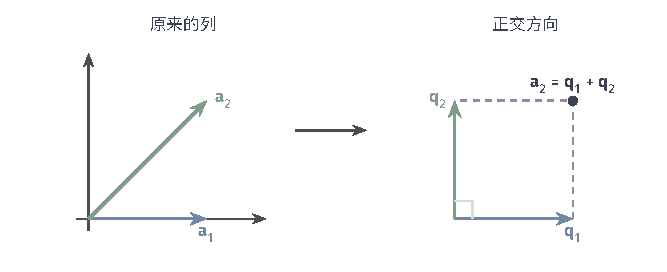
\includegraphics[width=112mm]{figures/00-shared/mathematical-preliminaries-upper/02-linear-spaces/tikz/comprehension-additions/linear-qr-columns.pdf}
  \caption{QR把列的方向和组合系数分开。取$\bm a_1=(1,0)^\top$、$\bm a_2=(1,1)^\top$，
  正交化得到$\bm q_1=(1,0)^\top$、$\bm q_2=(0,1)^\top$，并有$\bm a_1=\bm q_1$、
  $\bm a_2=\bm q_1+\bm q_2$，故$\bm R=\left[\begin{smallmatrix}1&1\\0&1\end{smallmatrix}\right]$。
  虚线补出第二列的分量。}
  \label{fig:vol1-add-linear-qr-columns}
\end{figure}

这一分解的用处在于，涉及列空间的计算可以改在标准正交的$\bm Q$上进行，坐标由内积直接读出，不必再解Gram方程；第~\ref{chap:linear-equations-and-optimization}章解方程与最小二乘问题时正是这样使用它的。

\subsubsection{列相关时的处理}

定理~\ref{thm:ls-gram-schmidt}要求各列线性无关。若不满足，某一步会出现$\bm u_j=\bm0$：由正交分解，这恰好说明$\bm a_j$已在前面方向张成的空间中，没有带来新方向。这时不能对零向量归一化，应跳过这一列，只在$\bm R$中记下它的系数$\langle\bm a_j,\bm q_i\rangle$；跳过它不影响后续各列，因为张成的空间没有变。

全部处理完以后，留下的$\bm q$个数等于列空间的维数$r=\operatorname{rank}\bm A$，仍有$\bm A=\bm Q\bm R$，其中$\bm Q\in\mathbb R^{m\times r}$的列是列空间的标准正交基，$\bm R\in\mathbb R^{r\times d}$的各行从左到右第一个非零元的位置逐行右移；$r<d$时$\bm R$不是方阵，不能求逆。下面是最小的例子。
\begin{example}[列相关时跳过零余量]
\label{ex:ls-qr-dependent-columns}
给定：$\bm A=[\bm a_1\ \bm a_2]$，$\bm a_1=(1,0)^\top$、$\bm a_2=(2,0)^\top$。

计算：$\bm q_1=\bm a_1$。$\langle\bm a_2,\bm q_1\rangle=2$，扣除后$\bm u_2=\bm a_2-2\bm q_1=\bm0$，所以跳过$\bm a_2$，只在$\bm R$中记下系数$2$。于是$r=1$，
\[
\begin{gathered}
\bm Q=\begin{bmatrix}1\\0\end{bmatrix}\\
\bm R=\begin{bmatrix}1&2\end{bmatrix}\\
\bm Q\bm R=\begin{bmatrix}1&2\\0&0\end{bmatrix}=\bm A .
\end{gathered}
\]

结论：列空间仍是$x$轴，$\bm Q$的一列构成它的标准正交基，$\operatorname{rank}\bm A=1$。
\end{example}
于是在精确算术下，同一过程也给出列空间的一组标准正交基与矩阵的秩。有限精度下扣除后的余量很少恰好为零，怎样判断它“算作零”、怎样改写扣除顺序以减少正交性的损失，属于数值计算问题，在第~\ref{sec:ls-numerical-sensitivity}节讨论。

\subsection{正交投影}

标准正交基使子空间的分量可以逐一读出。把这些分量合在一起，就得到离原向量最近的子空间向量。

\paragraph{向子空间的正交分解}
若$\bm q_1,\ldots,\bm q_r$是子空间$U$的标准正交基，第~\ref{sec:ls-orthogonality}节正交直和中的Gram方程变成$\bm a=(\langle\bm q_i,\bm x\rangle)_i$，分解直接写出：
\begin{equation}
 \bm x=\underbrace{\sum_{j=1}^r\langle\bm x,\bm q_j\rangle\bm q_j}_{\bm u\in U}+\underbrace{\Bigl(\bm x-\sum_{j=1}^r\langle\bm x,\bm q_j\rangle\bm q_j\Bigr)}_{\bm r\in U^\perp}.
 \label{eq:ls-orthonormal-projection}
\end{equation}
$\bm u$称为$\bm x$在$U$上的正交投影。$\bm u$与$\bm r$正交，由勾股定理$\lVert\bm x\rVert^2=\lVert\bm u\rVert^2+\lVert\bm r\rVert^2\geq\sum_{j=1}^r\langle\bm x,\bm q_j\rangle^2$：沿一部分标准正交方向读出的系数平方和不超过总长度的平方，等号恰在$\bm x\in U$时成立。对任意$\bm v\in U$，$\bm x-\bm v=(\bm x-\bm u)+(\bm u-\bm v)$的两项分别属于$U^\perp$和$U$。由勾股定理，
\[
 \lVert\bm x-\bm v\rVert^2=\lVert\bm x-\bm u\rVert^2+\lVert\bm u-\bm v\rVert^2\geq\lVert\bm x-\bm u\rVert^2.
\]
等号只在$\bm v=\bm u$时成立，所以$\bm u$是唯一的最近点。一般范数下的最近点可能不唯一；这里的唯一性来自内积所确定的正交分解。

在欧氏坐标下，把$\bm q_1,\ldots,\bm q_r$排成矩阵$\bm Q$，投影写成$P\bm x=\bm Q\bm Q^\top\bm x$。由于$\bm Q^\top\bm Q=\bm I$，投影矩阵$\bm P=\bm Q\bm Q^\top$满足$\bm P^2=\bm P$与$\bm P^\top=\bm P$：投影一次后再投影不再改变结果，配对中也可以把投影移到另一侧。$\bm Q$不是方阵时，$\bm P$通常不是整个空间的单位矩阵，它只保留$U$中的分量。非正交基同样可以通过前面得到的Gram方程计算投影；实际求解时不必显式形成逆矩阵。

\begin{example}[用标准正交基重算正交分解]
\label{ex:ls-orthonormal-projection-line}
给定：$U=\operatorname{span}\{\bm q_1\}$，$\bm q_1=(1,1,1)^\top/\sqrt3$，$\bm y=(1,1.1,0.9)^\top$。

计算：$\langle\bm y,\bm q_1\rangle=3/\sqrt3=\sqrt3$，投影为$\sqrt3\,\bm q_1=(1,1,1)^\top$，余量为$(0,0.1,-0.1)^\top$，它与$\bm q_1$正交。

结论：结果与示例~\ref{ex:ls-orthogonal-decomposition-line}相同，但这里不需要解Gram方程。
\end{example}
标准正交基让投影系数可以逐个读出，接下来把这一投影看作线性映射。

\paragraph{投影矩阵}
\label{sec:ls-projection-matrices}

求出的最近点随目标线性变化：$\bm y_1,\bm y_2$的正交分解相加、数乘后仍是正交分解，由分解的唯一性，
最近点也随之相加、数乘。所以$\bm y\mapsto\bm p$是一个线性映射，称为到$U$的正交投影。
本部分把它写成矩阵，并回答：拿到一个矩阵，怎样判断它是不是正交投影。

\paragraph{正交投影、斜投影与幂等}

设$\bm Q$的列是$U$的标准正交基。由$\bm p=\sum_j\langle\bm q_j,\bm y\rangle\bm q_j=\bm Q\bm Q^\top\bm y$，
标准内积下到$U$的正交投影是
\begin{equation}
\begin{gathered}
\bm P_U=\bm Q\bm Q^\top\\
\bm P_U^\top=\bm P_U\\
\bm P_U^2=\bm P_U.
\end{gathered}
\label{eq:linear-algebra-orthogonal-projector}
\end{equation}
两条性质都可以直接验证。由$\bm Q^\top\bm Q=\bm I$，$\bm P_U^2=\bm Q(\bm Q^\top\bm Q)\bm Q^\top=\bm Q\bm Q^\top$，
即幂等：已经在$U$中的点再投影一次不变。$(\bm Q\bm Q^\top)^\top=\bm Q\bm Q^\top$，即对称。
此外$\operatorname{range}\bm P_U=\operatorname{range}\bm Q=U$。

幂等性只说明这是某种投影，并不说明是最近点映射。一般的幂等矩阵$\bm P$把$\bm y$分成$\bm P\bm y$与
$\bm y-\bm P\bm y$两部分，前者在像中，后者在零空间中（因为$\bm P(\bm y-\bm P\bm y)=\bm P\bm y-\bm P^2\bm y=\bm0$），
但两部分不必正交。这种映射称为\term{斜投影}（oblique projection）。

\begin{example}[反例：幂等而不对称的投影]
\label{ex:ls-oblique-projection}
取$\bm P=\left[\begin{smallmatrix}1&-1\\0&0\end{smallmatrix}\right]$。直接相乘得$\bm P^2=\bm P$，所以它幂等；
它把$(y_1,y_2)^\top$送到$x$轴上的$(y_1-y_2,0)^\top$。残差$\bm y-\bm P\bm y=(y_2,y_2)^\top$与$x$轴方向$(1,0)^\top$的内积是$y_2$，
$y_2\neq0$时不为零，所以$\bm P\bm y$不是$x$轴上离$\bm y$最近的点。这个$\bm P$也不对称：$\bm P^\top\neq\bm P$。
\end{example}

对称性正是正交的条件：若$\bm P$幂等且对称，对任意$\bm y,\bm z$有
$(\bm y-\bm P\bm y)^\top\bm P\bm z=\bm y^\top(\bm P-\bm P^\top\bm P)\bm z=\bm y^\top(\bm P-\bm P^2)\bm z=0$，
残差与整个像正交，由正交性判据，$\bm P$就是到其像的正交投影。
所以判别分两步：先验幂等，判断是不是投影；再验对称，判断是不是正交投影。

\section{线性泛函的内积表示与伴随}
\label{sec:ls-adjoints}

第~\ref{sec:ls-dual-spaces}节的读取规则属于对偶空间，与被读取的向量不在同一个空间；转置在那里是对偶映射的矩阵。有了内积，读取可以写成与一个固定向量的配对，对偶映射也就变成内积空间之间的映射，称为伴随。第~\ref{sec:ls-orthogonality}节证明四个基本子空间的正交关系时，用到的正是它在欧氏内积下的形式：作用在左侧向量上的$\bm A$可以改写成作用在右侧向量上的$\bm A^\top$。第~\ref{chap:linear-analysis}章的对称矩阵与谱分解、第~\ref{chap:linear-equations-and-optimization}章的加权最小二乘，都要用到这种搬动。

\subsection{线性泛函的内积表示}
\phantomsection
\label{sec:ls-riesz-representation}
在$\mathbb R^d$的欧氏内积下，加权读取$\varphi(\bm x)=\bm a^\top\bm x$就是与向量$\bm a$的内积。一般有限维内积空间中，每个读取也都能这样写。
\begin{theorem}[有限维Riesz表示定理]
\label{thm:ls-riesz-representation}
设$V$是有限维内积空间。对每个$\varphi\in V^*$，存在唯一的$\bm v_\varphi\in V$，使$\varphi(\bm x)=\langle\bm x,\bm v_\varphi\rangle$对所有$\bm x\in V$成立。
\end{theorem}
\begin{proof}
取$V$的一组标准正交基$\bm q_1,\ldots,\bm q_d$（第~\ref{sec:ls-orthonormal-basis-construction}节），令$\bm v_\varphi=\sum_j\varphi(\bm q_j)\bm q_j$。由式~\eqref{eq:ls-orthonormal-expansion}，$\bm x=\sum_j\langle\bm x,\bm q_j\rangle\bm q_j$，于是
\[
 \varphi(\bm x)=\sum_j\langle\bm x,\bm q_j\rangle\varphi(\bm q_j)=\Bigl\langle\bm x,\sum_j\varphi(\bm q_j)\bm q_j\Bigr\rangle=\langle\bm x,\bm v_\varphi\rangle.
\]
若$\bm v,\bm v'$都满足要求，则$\langle\bm x,\bm v-\bm v'\rangle=0$对一切$\bm x$成立，取$\bm x=\bm v-\bm v'$得$\bm v=\bm v'$。
\end{proof}
对应$\varphi\mapsto\bm v_\varphi$保持线性组合（由表示向量的唯一性），并且每个$\bm v$都表示读取$\langle\cdot,\bm v\rangle$，所以它是$V^*$到$V$的双射。在它之下，标准正交基的对偶基就是这组基本身，因为第$j$个坐标读取是$\bm x\mapsto\langle\bm x,\bm q_j\rangle$。对一般的基，对偶基对应的向量与原基不同：图~\ref{fig:ls-dual-basis-readout}中的红色箭头$\bm b^1,\bm b^2$正是对偶读取$\varphi_1,\varphi_2$在欧氏内积下对应的向量。

表示向量依赖内积，读取本身却不依赖。在$\mathbb R^d$上取加权内积$\langle\bm x,\bm y\rangle_{\bm M}=\bm x^\top\bm M\bm y$，同一个读取$\varphi(\bm x)=\bm a^\top\bm x=\bm x^\top\bm M(\bm M^{-1}\bm a)$对应的向量是$\bm M^{-1}\bm a$，而不是$\bm a$。函数空间中也是如此。
\begin{example}[积分读取在两点内积下的表示向量]
\label{ex:ls-riesz-integral-two-point}
给定：$P_1$上的内积$\langle f,g\rangle=f(0)g(0)+f(1)g(1)$与读取$\varphi(f)=\int_0^1f(t)\,\mathrm dt$。

计算：对$f=a+bt$，$\varphi(f)=a+b/2$。另一方面，$f$与常数函数$\tfrac12$的内积为
\[
 \Bigl\langle f,\tfrac12\Bigr\rangle=\tfrac12\bigl(f(0)+f(1)\bigr)=\tfrac12(a+a+b)=a+\frac b2 .
\]

结论：$\bm v_\varphi$是常数函数$\tfrac12$。这也说明梯形公式$\tfrac12\bigl(f(0)+f(1)\bigr)$对一次函数精确。
\end{example}
表示向量还给出读取的大小。由Cauchy--Schwarz不等式，$|\varphi(\bm x)|\leq\lVert\bm x\rVert\,\lVert\bm v_\varphi\rVert$；$\bm v_\varphi\neq\bm0$时取$\bm x=\bm v_\varphi/\lVert\bm v_\varphi\rVert$可取到等号，所以第~\ref{sec:ls-finite-dimensional-sequences}节定义的$\lVert\varphi\rVert_*$等于$\lVert\bm v_\varphi\rVert$。

\subsection{伴随与特殊线性算子}
对偶映射把输出端的读取$f$传回输入端，得到读取$f\circ T$。若把读取都换成表示它的向量，就得到下面的定义。

设$T:V\to W$是两个有限维实内积空间之间的线性映射。若存在$T^\star:W\to V$使
\begin{equation}
 \langle T\bm x,\bm y\rangle_W=\langle\bm x,T^\star\bm y\rangle_V
 \label{eq:ls-adjoint-pairing}
\end{equation}
对所有$\bm x\in V$、$\bm y\in W$成立，则$T^\star$称为$T$的\term{伴随}（adjoint）。
\label{def:linear-algebra-adjoint}

伴随总存在且唯一。固定$\bm y\in W$，$\bm x\mapsto\langle T\bm x,\bm y\rangle_W$是$V$上的线性泛函，由定理~\ref{thm:ls-riesz-representation}，存在唯一的向量使它写成与该向量的内积，把这个向量记为$T^\star\bm y$。$T^\star$对$\bm y$线性：$\langle\bm x,aT^\star\bm y+bT^\star\bm y'\rangle_V=a\langle T\bm x,\bm y\rangle_W+b\langle T\bm x,\bm y'\rangle_W=\langle T\bm x,a\bm y+b\bm y'\rangle_W$，由表示向量的唯一性，$T^\star(a\bm y+b\bm y')=aT^\star\bm y+bT^\star\bm y'$。

用对偶映射的语言说，若把$\bm y\in W$看成读取$\langle\cdot,\bm y\rangle_W$，则$T'$把它送到读取$\langle T\,\cdot,\bm y\rangle_W=\langle\cdot,T^\star\bm y\rangle_V$：伴随就是借内积把读取换成向量以后的对偶映射。

具体计算时取$V,W$的基。由坐标下的内积公式，两边的内积写成$\langle\bm x,\bm x'\rangle_V=\bm x^\top\bm M_V\bm x'$、$\langle\bm y,\bm y'\rangle_W=\bm y^\top\bm M_W\bm y'$（这里$\bm x,\bm y$等指坐标），其中$\bm M_V,\bm M_W$是两组基的Gram矩阵，对称正定因而可逆；设$T$的矩阵为$\bm A$，伴随的矩阵为$\bm B$。式~\eqref{eq:ls-adjoint-pairing}要求$(\bm A\bm x)^\top\bm M_W\bm y=\bm x^\top\bm M_V\bm B\bm y$对所有$\bm x,\bm y$成立；取$\bm x,\bm y$为标准坐标向量逐个比较元素，这等价于$\bm A^\top\bm M_W=\bm M_V\bm B$，即
\begin{equation}
 \bm B=\bm M_V^{-1}\bm A^\top\bm M_W.
 \label{eq:ls-weighted-adjoint}
\end{equation}
两端都取标准正交基时，$\bm M_V,\bm M_W$都是单位矩阵，伴随矩阵就是$\bm A^\top$，与对偶映射的矩阵相同；两边权重不同时，伴随既不是单纯转置，也不是转置再求逆。下面的例子说明这一点。
\begin{example}[加权内积下的伴随]
\label{ex:ls-weighted-adjoint}
给定：$V=W=\mathbb R^2$都取加权内积$\langle\bm x,\bm y\rangle_{\bm M}=\bm x^\top\bm M\bm y$，$\bm M=\operatorname{diag}(4,1)$；$T\bm x=\bm A\bm x$，$\bm A=\left[\begin{smallmatrix}0&1\\0&0\end{smallmatrix}\right]$。

计算：由式~\eqref{eq:ls-weighted-adjoint}，
\[
 \bm B=\bm M^{-1}\bm A^\top\bm M
 =\begin{bmatrix}1/4&0\\0&1\end{bmatrix}\begin{bmatrix}0&0\\1&0\end{bmatrix}\begin{bmatrix}4&0\\0&1\end{bmatrix}
 =\begin{bmatrix}0&0\\4&0\end{bmatrix}.
\]
直接核对：$\bm A\bm x=(x_2,0)^\top$，$\langle\bm A\bm x,\bm y\rangle_{\bm M}=4x_2y_1$；$\bm B\bm y=(0,4y_1)^\top$，$\langle\bm x,\bm B\bm y\rangle_{\bm M}=x_2\cdot4y_1$，两者相等。

结论：伴随矩阵是$\left[\begin{smallmatrix}0&0\\4&0\end{smallmatrix}\right]$，而不是$\bm A^\top=\left[\begin{smallmatrix}0&0\\1&0\end{smallmatrix}\right]$。
\end{example}
对偶映射的矩阵总是$\bm A^\top$，差别来自读取与向量之间的对应$\bm a\mapsto\bm M^{-1}\bm a$随内积改变。四个基本子空间正交关系的证明只用到配对恒等式，所以对一般内积空间同样有$\ker T^\star=(\operatorname{im}T)^\perp$、$\ker T=(\operatorname{im}T^\star)^\perp$。

\paragraph{伴随的运算规则}
伴随与组合的规则由配对定义逐项推出：
\[
 \begin{gathered}
(T+S)^\star=T^\star+S^\star\\
(cT)^\star=c\,T^\star\\
(TS)^\star=S^\star T^\star\\
T^{\star\star}=T.
 \end{gathered}
\]
例如$\langle TS\bm x,\bm y\rangle=\langle S\bm x,T^\star\bm y\rangle=\langle\bm x,S^\star T^\star\bm y\rangle$，复合伴随的次序与乘积转置一样反转；恒等映射的伴随是自身。图~\ref{fig:ls-adjoint-action-transfer}把这种配对方向的搬回画成示意图。

伴随也不是逆：逆把输出复原成输入，伴随只把读取方向换一侧。
\begin{example}[反例：伴随不是逆]
\label{ex:ls-adjoint-not-inverse}
给定：非零内积空间$V$上的算子$T=2\operatorname{id}$。

验证：$\langle2\bm x,\bm y\rangle=\langle\bm x,2\bm y\rangle$对一切$\bm x,\bm y$成立，所以$T^\star=2\operatorname{id}$；而$T^{-1}=\tfrac12\operatorname{id}$。

结论：$T^\star\neq T^{-1}$。
\end{example}
\begin{figure}[!htb]
  \centering
  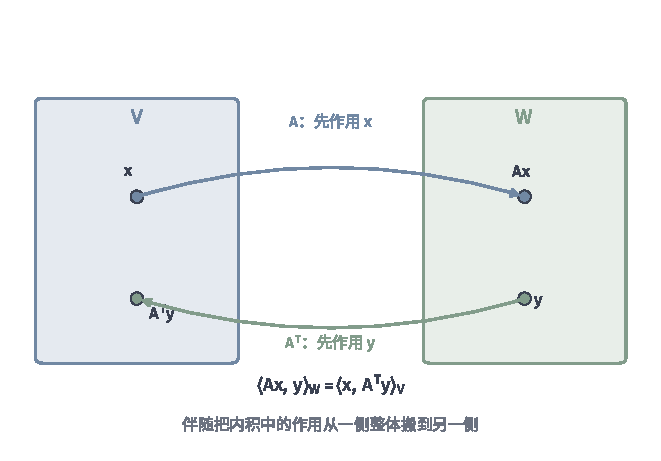
\includegraphics[width=112mm]{figures/00-shared/mathematical-preliminaries-upper/02-linear-spaces/matplotlib/ls-adjoint-action-transfer/ls-adjoint-action-transfer.pdf}
  \caption{内积伴随把输出端的配对搬回输入端。左：$T:V\to W$把$\bm x$映成$T\bm x$，与$\bm y\in W$配对；右：伴随$T^\star:W\to V$把$\bm y$映回$T^\star\bm y\in V$，使$\langle T\bm x,\bm y\rangle_W=\langle\bm x,T^\star\bm y\rangle_V$。标准欧氏内积下$T^\star$就是转置，是配对方向的反转而非逆作用。箭头与空间为解析示意。}
  \label{fig:ls-adjoint-action-transfer}
\end{figure}

\paragraph{自伴、正交与正规算子}
对算子$T:V\to V$，伴随仍是$V$上的算子，可以与$T$比较。若$T^\star=T$，称$T$为\term{自伴}（self-adjoint）算子，标准坐标下对应对称矩阵。若$Q^\star Q=\operatorname{id}$，则$Q$保持内积：$\langle Q\bm x,Q\bm y\rangle=\langle\bm x,Q^\star Q\bm y\rangle=\langle\bm x,\bm y\rangle$，称为正交算子；标准坐标下它对应第~\ref{sec:ls-orthogonal-matrices}节的正交矩阵，且由方阵的单侧逆即双侧逆，$Q^{-1}=Q^\star$。满足$TT^\star=T^\star T$的算子称为\term{正规}（normal）算子，自伴与正交都属于它。这些类别的谱性质在第~\ref{chap:linear-analysis}章展开，这里只给出定义。

\paragraph{复空间中的泛函表示与伴随}
复空间沿用前述“第一变量共轭线性、第二变量线性”的约定。线性泛函应写成$\varphi(\bm x)=\langle\bm v,\bm x\rangle$：$\bm x$处于线性槽位。若$\bm q_1,\ldots,\bm q_d$是标准正交基，则$\bm v=\sum_j\overline{\varphi(\bm q_j)}\bm q_j$；直接代入各基向量可核对其读数。表示向量随泛函作共轭线性变化，与实空间中的线性对应不同。

例如在$\mathbb C$的标准内积$\langle v,z\rangle=\overline v z$下，泛函$\varphi(z)=(1+\mathrm i)z$对应$ v=1-\mathrm i$。代入便有$\overline v z=(1+\mathrm i)z$；若把两个槽位交换，就会得到关于$z$共轭线性的表达式。这个一维核验说明，共轭来自内积约定，不能从实数公式中直接删去。

两个复内积空间之间的伴随满足$\langle T\bm x,\bm y\rangle_W=\langle\bm x,T^\star\bm y\rangle_V$。在标准正交基下，$T$的矩阵若为$\bm A$，伴随的矩阵就是$\bm A^*$；若两端基的Gram矩阵为$\bm M_V,\bm M_W$，则为$\bm M_V^{-1}\bm A^*\bm M_W$。这与代数对偶映射的矩阵$\bm A^\top$不同：后者只复合线性泛函，不涉及内积和共轭。复空间中自伴矩阵满足$\bm A=\bm A^*$，保内积的方阵满足$\bm A^*\bm A=\bm I$，称为酉矩阵。

\section{本章小结}
\label{sec:ls-normed-inner-product-summary}

范数给向量规定大小，从而可以比较误差并定义收敛。有限维空间中的范数彼此等价，向量列收敛等价于逐坐标收敛；这些空间及其子空间都是完备的。对偶范数把输入大小的限制转化为线性泛函的最大读数，商范数则衡量忽略一个子空间中的差别以后剩余的大小。

内积进一步给出角度和正交。Gram矩阵记录一组向量的两两内积，正交分解把向量拆成子空间内的部分与垂直部分；正交投影是内积诱导距离下唯一的最近点。标准正交基简化配对与坐标计算，线性泛函的内积表示和伴随则连接了上一章的代数对偶与本章的几何结构。

这些结论为下一章寻找线性作用的简单表示提供了工具。有限维中的闭性、完备性和连续性不能不加条件地推广到无限维空间。


\chapter{谱和奇异值}
\label{chap:linear-analysis}
\label{chap:matrix-analysis}

第~\ref{chap:linear-representation}章说明，矩阵记录的是线性映射在一组基下的坐标；对线性算子，输入、输出两端换成同一组新基时，矩阵按相似关系$\bm B=\bm P^{-1}\bm A\bm P$改变（第~\ref{sec:ls-similarity}节）。因此同一个作用有许多种矩阵写法，有的繁杂，有的简单。那里的例子已经显示，算子$T(x_1,x_2)=(2x_1+x_2,3x_2)$在标准基下的矩阵有非零的非对角元，换到合适的基以后却成了对角矩阵，原因是新的两个基方向在作用下只被伸缩、不被转向。本章围绕一个问题展开：一个线性作用在什么样的基下最简单，从这个最简形式又能读出它的哪些性质？

前五节回答第一问。最理想的基由只被伸缩的方向组成。第~\ref{sec:ls-linear-operators}节寻找这样的方向，即特征向量；相应的伸缩倍数称为特征值。特征值不随基改变，可以由特征多项式系统地求出；把矩阵代入自身的特征多项式总得到零矩阵，这就是Cayley--Hamilton定理。第~\ref{sec:ls-matrix-powers}节判断特征向量何时足以组成一组基。这时矩阵经可逆矩阵相似于对角矩阵，矩阵幂化为对角元的乘方；实特征值不够或特征向量不够时，矩阵不能对角化。

对角化所用的基未必互相垂直，换到这组基时长度和夹角都会变形。于是第~\ref{sec:ls-spectral-theory}节进一步要求换基矩阵是正交矩阵，证明能这样对角化的恰好是实对称矩阵，并由此得到特征值的极值刻画与矩阵函数。一般方阵可能缺少实特征向量，特征向量也可能互不正交。第~\ref{sec:ls-general-square-spectrum}节说明，坚持用正交矩阵换基时，一般方阵最多化为分块上三角的实Schur形，恰好能化为分块对角形的是正规矩阵；该节还引入概括伸缩倍数的谱半径。最后放宽“输入、输出用同一组基”的要求：两端各取一组标准正交基时，任何矩阵，包括矩形矩阵，都能化为对角形，这就是第~\ref{sec:ls-svd}节的奇异值分解。

后三节用这些最简形式回答第二问。第~\ref{sec:ls-perturbation}节研究一次作用对输入误差的放大，最大奇异值给出绝对误差的一步最大放大倍数；最大与最小奇异值之比，即条件数，刻画相对误差可能受到的放大。第~\ref{sec:ls-spectral-sensitivity}节把矩阵本身当作输入，估计矩阵受到扰动时特征值、奇异值和特征子空间移动多少。第~\ref{sec:ls-convergence}节研究反复作用：矩阵幂与矩阵级数的长期行为由谱决定，早期的放大则取决于矩阵是否正规。本章的结论随后用于第~\ref{chap:linear-equations-and-optimization}章：那里求解线性方程、最小二乘与矩阵方程时，伪逆由奇异值分解构造，解的敏感度由条件数衡量，Sylvester方程与Lyapunov方程的可解性则依赖谱、Cayley--Hamilton定理与实Schur形。

% 第6章第1节：特征值与特征向量（特征方向、特征空间、特征多项式与Cayley--Hamilton定理、相似不变性、不同特征值的特征向量）。

\section{特征值与特征向量}
\label{sec:ls-linear-operators}

第~\ref{sec:ls-similarity}节的例子已经显示，算子$T(x_1,x_2)=(2x_1+x_2,3x_2)$在标准基下的矩阵有非零的非对角元，换到新基$\bm b_1'=\bm e_1$、$\bm b_2'=\bm e_1+\bm e_2$以后却成了对角矩阵$\operatorname{diag}(2,3)$。原因在于，这两个基方向在作用下只被伸缩、不被转向。

不过，那组新基是事先给出、再加以验证的。要为一般的算子找出这样的基，需要依次回答四个问题：只被伸缩的方向怎样寻找，伸缩倍数怎样求出，它们是否随基改变，彼此线性无关的这类方向最多有多少个。

\subsection{线性作用中的特征方向}
\label{sec:ls-operator-eigenvectors}

第~\ref{sec:ls-linear-map-definition}节说明，线性算子$T:V\to V$总把原点留在原处，但一般会同时改变向量的长度和方向。于是可以问：有没有非零向量在作用以后仍落在原来那条过原点的直线上，只被伸长、缩短或反向，而不被转到别的方向？用等式表达，就是要求非零向量$\bm v\in V$与实数$\lambda$满足
\begin{equation}
\begin{gathered}
T\bm v=\lambda\bm v\\
\bm v\neq\bm0.
\end{gathered}
\label{eq:matrix-analysis-eigenpair}
\end{equation}
这时称$\lambda$为$T$的\term{特征值}（eigenvalue），$\bm v$为属于$\lambda$的\term{特征向量}（eigenvector），$\bm v$所在的直线称为\term{特征方向}。

特征值说明这条直线上发生了什么：$|\lambda|>1$时向量被拉长，$|\lambda|<1$时被缩短，$\lambda<0$时方向还被反过来，$\lambda=0$则表示$T\bm v=\bm0$，即$\bm v$在$T$的核中。

定义要求特征向量非零，因为零向量对任何$\lambda$都满足$T\bm0=\lambda\bm0$，不提供方向信息。

在特征方向上，反复作用也最简单。第~\ref{sec:ls-operator-powers}节说明，算子可以与自身复合，得到$T^k$。对特征向量$\bm v$，由$T\bm v=\lambda\bm v$与线性性得$T^2\bm v=T(\lambda\bm v)=\lambda T\bm v=\lambda^2\bm v$，归纳即得$T^k\bm v=\lambda^k\bm v$。所以在这条直线上，$k$次作用化为数$\lambda$的$k$次乘方；在一般方向上，矩阵幂则会不断混合各个坐标。

特征值是算子本身的性质，不依赖基的选取。取一组基$\mathcal B$后，式~\eqref{eq:matrix-analysis-eigenpair}的坐标形式是$[T]_{\mathcal B}[\bm v]_{\mathcal B}=\lambda[\bm v]_{\mathcal B}$。等式两侧分别是向量$T\bm v$与$\lambda\bm v$的坐标，而$\bm v\neq\bm0$当且仅当它的坐标非零。所以无论取哪组基，矩阵$[T]_{\mathcal B}$的特征值都恰好是$T$的特征值；换基只改变特征向量的坐标。

对$n$阶方阵$\bm A$，它的特征值与特征向量指算子$\bm x\mapsto\bm A\bm x$的特征值与特征向量，即满足$\bm A\bm v=\lambda\bm v$、$\bm v\neq\bm0$的$\lambda$与$\bm v$。

回到开头的算子，可以直接验证哪些方向是特征方向。
\begin{example}[验证特征向量]
\label{ex:ls-operator-eigenvector-check}
给定算子$T(x_1,x_2)=(2x_1+x_2,3x_2)$，它在标准基下的矩阵为
\[
 \bm A=\begin{bmatrix}2&1\\0&3\end{bmatrix}.
\]
检验$\bm e_1$、$(1,1)^{\top}$与$\bm e_2$是否为特征向量。直接相乘得
\[
\begin{gathered}
\bm A\bm e_1=\begin{bmatrix}2\\0\end{bmatrix}=2\bm e_1\\
\bm A\begin{bmatrix}1\\1\end{bmatrix}=\begin{bmatrix}3\\3\end{bmatrix}=3\begin{bmatrix}1\\1\end{bmatrix}\\
\bm A\bm e_2=\begin{bmatrix}1\\3\end{bmatrix}.
\end{gathered}
\]
结论：$\bm e_1$与$(1,1)^{\top}$是特征向量，特征值分别为$2$和$3$，它们正是第~\ref{sec:ls-similarity}节新基的两个方向；$(1,3)^{\top}$不是$\bm e_2$的倍数，所以$\bm e_2$不是特征向量。
\end{example}
图~\ref{fig:ls-operator-eigenvectors}画出这个例子：两条特征方向上的向量作用后仍在原直线上，只是变长；其他方向上的向量则被转开。
\begin{figure}[!htb]
  \centering
  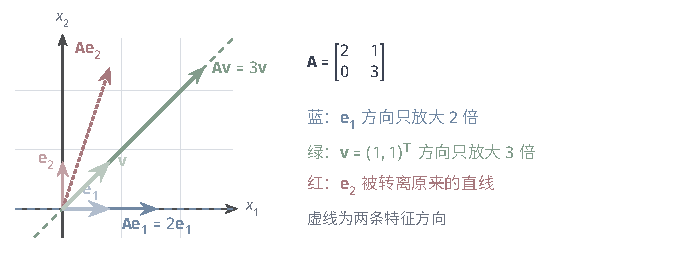
\includegraphics[width=112mm]{figures/00-shared/mathematical-preliminaries-upper/02-linear-spaces/tikz/comprehension-additions/operator-eigenvectors.pdf}
  \caption{特征向量只被伸缩、不被转向。算子$T(x_1,x_2)=(2x_1+x_2,3x_2)$在标准基下的矩阵为$\bm A=\left[\begin{smallmatrix}2&1\\0&3\end{smallmatrix}\right]$，它把$\bm e_1$送到$2\bm e_1$，把$\bm v=(1,1)^{\top}$送到$3\bm v$，二者都留在各自的虚线上；$\bm e_2$被送到$(1,3)^{\top}$，偏离了原来的直线，所以不是特征向量。}
  \label{fig:ls-operator-eigenvectors}
\end{figure}

并非每个算子都有实特征向量。下面的反例中，每个非零向量都被转离原来的直线。
\begin{example}[反例：平面旋转没有实特征向量]
\label{ex:ls-rotation-no-real-eigenvector}
给定平面上逆时针旋转$90^\circ$的算子$R(x_1,x_2)=(-x_2,x_1)$。检验它是否有实特征值。设实数$\lambda$与向量$(x_1,x_2)$满足$R(x_1,x_2)=\lambda(x_1,x_2)$，即
\[
 \begin{gathered}
-x_2=\lambda x_1\\
x_1=\lambda x_2 .
 \end{gathered}
\]
把第二式代入第一式得$-x_2=\lambda^2x_2$，即$(1+\lambda^2)x_2=0$。由于$1+\lambda^2>0$，只能$x_2=0$，进而$x_1=\lambda x_2=0$。结论：对任何实数$\lambda$，满足等式的只有零向量，所以$R$没有实特征值，也没有实特征向量。
\end{example}

\subsection{特征空间与不变子空间}

同一个特征值往往不止对应一条特征方向。固定特征值$\lambda$，满足$T\bm v=\lambda\bm v$的全部向量连同零向量组成集合$\ker(T-\lambda\,\operatorname{id}_V)$，称为$\lambda$的\term{特征空间}（eigenspace）。它是一个线性映射的核，因而是子空间。

例如$\bm I_2$的每个非零向量都是属于$1$的特征向量，特征空间是整个平面；而示例~\ref{ex:ls-operator-eigenvector-check}中属于$2$的特征空间只是$\bm e_1$所在的直线，因为$\bm A-2\bm I=\left[\begin{smallmatrix}0&1\\0&1\end{smallmatrix}\right]$的核由第二坐标为零的向量组成。

特征空间是一类更一般的子空间的特例。若子空间$S$满足$T(S)\subseteq S$，就称$S$为$T$的\term{不变子空间}（invariant subspace）。这时作用不会把$S$中的向量带出$S$，于是可以把$T$限制在$S$上单独研究。特征空间是不变子空间，因为其中的向量只被乘以$\lambda$，仍留在其中。

一维不变子空间恰好就是特征方向。若$\bm v\neq\bm0$且$\operatorname{span}\{\bm v\}$不变，则$T\bm v$落在这条直线上，是$\bm v$的倍数；反之，若$T\bm v=\lambda\bm v$，则$T(c\bm v)=\lambda c\bm v$仍在这条直线上。高于一维的不变子空间却未必含有特征方向：整个平面对$90^\circ$旋转不变，而示例~\ref{ex:ls-rotation-no-real-eigenvector}说明其中没有一条特征方向。第~\ref{sec:ls-general-square-spectrum}节将看到，这样的二维不变子空间对应一对共轭的复特征值。

\subsection{特征多项式}
\label{sec:ls-characteristic-polynomial}

示例~\ref{ex:ls-operator-eigenvector-check}中的特征向量是先猜出、再验证的。能否系统地求出全部特征值？对$n$阶方阵$\bm A$，$\lambda$是特征值，当且仅当齐次方程$(\bm A-\lambda\bm I)\bm v=\bm0$有非零解，即$\ker(\bm A-\lambda\bm I)\neq\{\bm0\}$。由第~\ref{sec:ls-injective-surjective-invertible}节的等价条件，这又等价于$\operatorname{rank}(\bm A-\lambda\bm I)<n$，也等价于$\bm A-\lambda\bm I$不可逆。

不可逆又等价于行列式为零，这一步用到第~\ref{sec:ls-determinant-properties}节的两条性质。若方阵$\bm M$可逆，乘法性给出$\det\bm M\det(\bm M^{-1})=\det\bm I=1$，故$\det\bm M\neq0$；反之若$\det\bm M\neq0$，古典伴随恒等式说明$\operatorname{adj}(\bm M)/\det\bm M$就是$\bm M$的逆。所以$\lambda$是$\bm A$的特征值，当且仅当$\det(\bm A-\lambda\bm I)=0$。第~\ref{sec:ls-similarity-properties}节把每个$\operatorname{rank}(\bm A-c\bm I)$都列为相似不变量；现在可以看出，使这个秩小于$n$的数$c$恰好就是特征值。

为了把这个条件写成首项系数为正的多项式，注意$\det(\lambda\bm I-\bm A)=(-1)^n\det(\bm A-\lambda\bm I)$，二者同时为零。定义
\begin{equation}
 p_{\bm A}(z)=\det(z\bm I-\bm A),
 \label{eq:matrix-analysis-characteristic-polynomial}
\end{equation}
称为\term{特征多项式}（characteristic polynomial），就得到：$\bm A$的实特征值恰为$p_{\bm A}$的实根。在行列式的排列展开中，对角线一项是$\prod_i(z-a_{i,i})$；其余每一项至少有两个因子取自非对角位置，含$z$的因子至多$n-2$个。所以只有对角线一项含$z^n$，$p_{\bm A}$是首项系数为$1$的$n$次实多项式，至多有$n$个不同的根。求出一个特征值$\lambda$以后，再解齐次方程$(\bm A-\lambda\bm I)\bm v=\bm0$，就得到它的特征空间。

用特征多项式可以重新求出前面两个例子的特征值，而不必猜测特征向量。
\begin{example}[用特征多项式求特征值]
\label{ex:ls-characteristic-polynomial-two-by-two}
给定示例~\ref{ex:ls-operator-eigenvector-check}的$\bm A=\left[\begin{smallmatrix}2&1\\0&3\end{smallmatrix}\right]$，以及示例~\ref{ex:ls-rotation-no-real-eigenvector}的旋转在标准基下的矩阵$\bm R=\left[\begin{smallmatrix}0&-1\\1&0\end{smallmatrix}\right]$。二者的特征多项式为
\[
 \begin{aligned}
 p_{\bm A}(z)&=\det\begin{bmatrix}z-2&-1\\0&z-3\end{bmatrix}=(z-2)(z-3),\\
 p_{\bm R}(z)&=\det\begin{bmatrix}z&1\\-1&z\end{bmatrix}=z^2+1 .
 \end{aligned}
\]
结论：$\bm A$的特征值为$2$与$3$，与示例~\ref{ex:ls-operator-eigenvector-check}验证的两条特征方向相符；$z^2+1$对任何实数$z$都为正，没有实根，所以$\bm R$没有实特征值，与示例~\ref{ex:ls-rotation-no-real-eigenvector}的直接验证一致。
\end{example}
$\bm A$的情形可以推广到任意三角矩阵：三角矩阵$\bm A$的$z\bm I-\bm A$仍是三角矩阵，行列式是对角元之积$\prod_i(z-a_{i,i})$，所以三角矩阵的特征值就是它的对角元。

特征多项式在每个特征值处取零。若把矩阵本身代入特征多项式，又会得到什么？这里的代入是指把多项式中的$z^j$换成$\bm A^j$，常数项$c_0$换成$c_0\bm I$。先看一个例子。
\begin{example}[把矩阵代入它的特征多项式]
\label{ex:ls-cayley-hamilton-two-by-two}
给定$\bm A=\left[\begin{smallmatrix}2&1\\0&3\end{smallmatrix}\right]$。由示例~\ref{ex:ls-characteristic-polynomial-two-by-two}，$p_{\bm A}(z)=(z-2)(z-3)=z^2-5z+6$。计算$p_{\bm A}(\bm A)=\bm A^2-5\bm A+6\bm I$：
\[
\begin{gathered}
\bm A^2=\begin{bmatrix}4&5\\0&9\end{bmatrix}\\
\bm A^2-5\bm A+6\bm I
 =\begin{bmatrix}4-10+6&5-5+0\\0&9-15+6\end{bmatrix}
 =\bm0 .
\end{gathered}
\]
结论：把$\bm A$代入自身的特征多项式，得到零矩阵。
\end{example}
这不是巧合。证明的工具是第~\ref{sec:ls-determinant-properties}节的古典伴随恒等式（定理~\ref{thm:ls-adjugate-identity}）$\bm M\operatorname{adj}(\bm M)=\det(\bm M)\bm I$。令$\bm M=z\bm I-\bm A$，得
\[
 (z\bm I-\bm A)\operatorname{adj}(z\bm I-\bm A)=p_{\bm A}(z)\bm I .
\]
$\operatorname{adj}(z\bm I-\bm A)$的每个元素都是$z\bm I-\bm A$的一个带符号的$n-1$阶余子式，它是$z$的多项式，次数不超过$n-1$。按$z$的幂次整理，可以写成$\operatorname{adj}(z\bm I-\bm A)=\sum_{j=0}^{n-1}z^j\bm B_j$，其中$\bm B_j$是不含$z$的常数矩阵。
\begin{theorem}[Cayley--Hamilton定理]
\label{thm:ls-cayley-hamilton}
设$n$阶方阵$\bm A$的特征多项式为$p_{\bm A}(z)=z^n+c_{n-1}z^{n-1}+\cdots+c_0$，则
\[
 p_{\bm A}(\bm A)
 =\bm A^n+c_{n-1}\bm A^{n-1}+\cdots+c_1\bm A+c_0\bm I=\bm0.
\]
\end{theorem}
\begin{proof}
把$\operatorname{adj}(z\bm I-\bm A)=\sum_{j=0}^{n-1}z^j\bm B_j$代入上式，左边为$\sum_jz^{j+1}\bm B_j-\sum_jz^j\bm A\bm B_j$。两边每个元素都是$z$的多项式，且对所有实数$z$相等，所以同次项的系数相等。记$c_n=1$，比较$z$的各次幂系数：
\[
 \begin{aligned}
 &z^n: &&\bm B_{n-1}=\bm I;\\
 &z^j\ (1\leq j\leq n-1): &&\bm B_{j-1}-\bm A\bm B_j=c_j\bm I;\\
 &z^0: &&-\bm A\bm B_0=c_0\bm I .
 \end{aligned}
\]
把$z^j$项的等式左乘$\bm A^j$（$j=0,\ldots,n$）后相加。右边恰为$\sum_jc_j\bm A^j=p_{\bm A}(\bm A)$；左边为
\[
 \bm A^n\bm B_{n-1}+\sum_{j=1}^{n-1}\bigl(\bm A^j\bm B_{j-1}-\bm A^{j+1}\bm B_j\bigr)-\bm A\bm B_0 ,
\]
其中相邻项逐对相消，总和为零。
\end{proof}
证明只用到行列式与古典伴随，既不需要先求出特征值，也不要求$p_{\bm A}$有实根。

定理的一个直接推论是，高次幂可以由低次幂表示。由$p_{\bm A}(\bm A)=\bm0$得$\bm A^n=-\sum_{j=0}^{n-1}c_j\bm A^j$，即$\bm A^n$是$\bm I,\bm A,\ldots,\bm A^{n-1}$的线性组合。两边再左乘$\bm A$，右端出现的$\bm A^n$同样用这个式子代换，可知$\bm A^{n+1}$也是这些矩阵的线性组合；归纳可得，所有$\bm A^k$（$k\geq n$）都是。因此，对任意向量$\bm g$，$\bm A^k\bm g$（$k\geq n$）都是$\bm g,\bm A\bm g,\ldots,\bm A^{n-1}\bm g$的线性组合，序列$\bm g,\bm A\bm g,\bm A^2\bm g,\ldots$张成的子空间在前$n$项之后不再增大。第~\ref{chap:linear-equations-and-optimization}章判断Sylvester方程何时有唯一解时，要用到这个定理。

同一个特征值可以是特征多项式的重根。这时，关于这个特征值有两种“个数”需要区分。根$\lambda$在$p_{\bm A}$中的重数称为\term{代数重数}（algebraic multiplicity），特征空间的维数$\dim\ker(\bm A-\lambda\bm I)$称为\term{几何重数}（geometric multiplicity）。下面的例子说明二者可以不同。
\begin{example}[代数重数大于几何重数]
\label{ex:ls-multiplicity-gap}
给定
\[
 \bm J=\begin{bmatrix}0.8&1\\0&0.8\end{bmatrix}.
\]
它是上三角矩阵，特征多项式为$p_{\bm J}(z)=(z-0.8)^2$，所以唯一的特征值$0.8$的代数重数为$2$。再求特征空间：
\[
\begin{gathered}
\bm J-0.8\bm I=\begin{bmatrix}0&1\\0&0\end{bmatrix}\\
(\bm J-0.8\bm I)\begin{bmatrix}x_1\\x_2\end{bmatrix}=\begin{bmatrix}x_2\\0\end{bmatrix},
\end{gathered}
\]
它为零当且仅当$x_2=0$，所以特征空间是$(1,0)^{\top}$所在的直线。结论：特征值$0.8$的代数重数为$2$，几何重数只有$1$。
\end{example}
两种重数的一般关系，以及它们怎样决定能否找到由特征向量组成的基，在第~\ref{sec:ls-matrix-powers}节讨论。对一般的算子$T$，可以取任一组基把它写成矩阵，再求特征多项式与两种重数；下一小节说明，这样得到的结果不依赖基的选取。

\subsection{相似变换与谱的不变性}
\label{sec:ls-eigen-similarity-invariance}

第~\ref{sec:ls-similarity-properties}节列出了相似保持的量：秩、零空间的维数、每个$\operatorname{rank}(\bm A-c\bm I)$，以及行列式与迹。特征值、特征多项式与两种重数是否也在其中？若是，它们就属于算子本身，可以用任意一组基下的矩阵计算。下面设$\bm B=\bm P^{-1}\bm A\bm P$，其中$\bm P$可逆。

先看特征值与几何重数。若$\bm A\bm v=\lambda\bm v$且$\bm v\neq\bm0$，则
\[
 \bm B(\bm P^{-1}\bm v)=\bm P^{-1}\bm A\bm P\bm P^{-1}\bm v=\bm P^{-1}\bm A\bm v=\lambda\bm P^{-1}\bm v .
\]
$\bm P$可逆保证$\bm P^{-1}\bm v\neq\bm0$，所以$\lambda$也是$\bm B$的特征值，相应的特征向量是$\bm P^{-1}\bm v$；交换$\bm A,\bm B$的角色即得反向结论。同样的计算说明$\ker(\bm B-\lambda\bm I)=\bm P^{-1}\ker(\bm A-\lambda\bm I)$，而可逆矩阵把子空间映成同维数的子空间，所以每个特征值的几何重数不变。这一结论也可以由式~\eqref{eq:ls-similarity-shifted-rank}取$c=\lambda$、再用秩零度定理换成核的维数得到。

更进一步，整个特征多项式不变：
\[
 p_{\bm B}(z)=\det(z\bm I-\bm P^{-1}\bm A\bm P)=\det\bigl(\bm P^{-1}(z\bm I-\bm A)\bm P\bigr)=p_{\bm A}(z),
\]
中间一步用了$z\bm I=\bm P^{-1}(z\bm I)\bm P$，最后一步用了第~\ref{sec:ls-similarity-properties}节的恒等式$\det(\bm P^{-1}\bm M\bm P)=\det\bm M$。所以算子的特征多项式可以用任意一组基下的矩阵计算，代数重数也是相似不变量。

特征多项式的系数还说明了行列式与迹为什么是相似不变量：它们就是$p_{\bm A}$的两个系数，至多差一个符号。令$z=0$，得常数项$p_{\bm A}(0)=\det(-\bm A)=(-1)^n\det\bm A$。再看$z^{n-1}$的系数。上一小节已经指出，排列展开中除对角线一项外，每一项含$z$的因子至多$n-2$个；所以$z^{n-1}$只来自$\prod_i(z-a_{i,i})$，系数为$-\sum_ia_{i,i}=-\operatorname{tr}\bm A$。于是
\[
 p_{\bm A}(z)=z^n-(\operatorname{tr}\bm A)\,z^{n-1}+\cdots+(-1)^n\det\bm A .
\]

若$p_{\bm A}$能分解为实一次因子之积$\prod_{i=1}^n(z-\lambda_i)$，其中每个特征值按代数重数重复列出，把右端展开后比较$z^{n-1}$的系数与常数项，得
\[
 \begin{gathered}
\operatorname{tr}\bm A=\sum_{i=1}^n\lambda_i\\
\det\bm A=\prod_{i=1}^n\lambda_i .
 \end{gathered}
\]
例如示例~\ref{ex:ls-operator-eigenvector-check}的$\bm A$有$\operatorname{tr}\bm A=5=2+3$，$\det\bm A=6=2\cdot3$。第~\ref{sec:ls-general-square-spectrum}节把特征多项式的复根也算作特征值以后，这两个等式对每个方阵都成立。

相似不变量只能用来否定相似：某个相似不变量不同，两个矩阵就不相似；不变量全部相同，两个矩阵却未必相似。第~\ref{sec:ls-similarity-conditions}节比较过$\bm I_2$与$\left[\begin{smallmatrix}1&1\\0&1\end{smallmatrix}\right]$，现在可以用特征值的语言重新说明二者为什么不相似。
\begin{example}[反例：特征多项式相同而不相似]
\label{ex:ls-same-charpoly-not-similar}
给定$\bm I_2$与
\[
 \bm J_1=\begin{bmatrix}1&1\\0&1\end{bmatrix}.
\]
二者都是上三角矩阵，对角元都是$1$，所以$p_{\bm I_2}(z)=p_{\bm J_1}(z)=(z-1)^2$，特征值$1$的代数重数都是$2$。另一方面，
\[
\begin{gathered}
\bm I_2-\bm I_2=\bm0\\
\bm J_1-\bm I_2=\begin{bmatrix}0&1\\0&0\end{bmatrix},
\end{gathered}
\]
前者的核是整个平面，后者的核只是$(1,0)^{\top}$所在的直线，几何重数分别为$2$与$1$。结论：二者的特征多项式相同，但几何重数不同；由于几何重数是相似不变量，它们不相似。
\end{example}
所以特征多项式相同只是相似的必要条件。比较各特征值的几何重数是更细的必要条件，但一般仍不足以判定相似；完整的相似分类需要Jordan标准形，本书不展开。下一节只处理最重要、也最常用的一类矩阵：与对角矩阵相似的矩阵。

\subsection{不同特征值对应方向的独立性}
\label{sec:ls-eigenvector-independence}

特征方向能否多到组成一组基？先要说明，属于不同特征值的特征向量不会彼此重复，即它们线性无关。

设$\bm v_1,\ldots,\bm v_r$分别属于互不相同的特征值$\lambda_1,\ldots,\lambda_r$，假设它们线性相关。在所有非平凡的线性依赖中取项数最少的一个，重新编号后记为$\sum_{j=1}^s c_j\bm v_j=\bm0$，其中各$c_j\neq0$；单个特征向量非零，不能单独构成依赖，所以$s\geq2$。两边作用$T-\lambda_1\operatorname{id}_V$：第一项变为零，其余各项变为$c_j(\lambda_j-\lambda_1)\bm v_j$。特征值互不相同，这些系数仍非零，于是得到一个只有$s-1$项的非平凡依赖，与$s$最少矛盾。所以$\bm v_1,\ldots,\bm v_r$线性无关。由于$n$维空间中线性无关的向量至多$n$个，$n$维空间上的算子至多有$n$个不同特征值，这与特征多项式的次数给出的上界一致。

由此，不同特征值的特征空间之和是直和。

设$\sum_\lambda\bm w_\lambda=\bm0$，每个$\bm w_\lambda$属于相应的特征空间；其中非零的$\bm w_\lambda$是属于不同特征值的特征向量，它们线性无关，所以只能每个$\bm w_\lambda=\bm0$。把各特征空间的基合在一起，它们的任一线性组合都可以按特征值分组写成$\sum_\lambda\bm w_\lambda$；若组合为零，则每个$\bm w_\lambda=\bm0$，而每组基本身线性无关，所以全部系数为零。因此各特征空间的基合在一起仍线性无关。

例如示例~\ref{ex:ls-operator-eigenvector-check}中的$\bm e_1$与$(1,1)^{\top}$属于不同的特征值$2$与$3$，不必另行验证，它们自动线性无关，在平面上组成一组基。

至此，本节开头的四个问题都有了回答。被算子只伸缩的方向是特征方向，伸缩倍数是特征值；特征值是特征多项式的实根，求出特征值后解齐次方程即得特征空间。特征值、特征多项式和两种重数都不随基改变，属于算子本身。属于不同特征值的特征向量线性无关，所以$n$维空间上的算子至多有$n$个不同特征值。

途中还得到了Cayley--Hamilton定理：$\bm A$的高次幂都能用$\bm I,\bm A,\ldots,\bm A^{n-1}$表示。剩下的问题是特征向量什么时候多到足以组成一组基，这是下一节的对角化问题。

% 第6章第2节：基于可逆矩阵的对角化（特征基下的矩阵与幂、可对角化的定义与判据及不能对角化的情形、步骤与算例）。

\section{对角化}
\label{sec:ls-matrix-powers}
\label{sec:ch06-powers-spectrum}

上一节找到了被算子只伸缩的方向，并证明属于不同特征值的特征向量线性无关。本节回答由此引出的问题：有了由特征向量组成的基，算子的矩阵变成什么样，又能怎样利用？这样的基什么时候存在？换到这组基所用的换基矩阵只要求可逆，不要求各列互相垂直，所以本节的对角化是用一般的可逆矩阵作相似变换。

\subsection{特征向量基下的矩阵表示}
\label{sec:matrix-analysis-spectrum}

设$\bm v_1,\ldots,\bm v_n$是由算子$T$的特征向量组成的基，$T\bm v_j=\lambda_j\bm v_j$。按第~\ref{sec:ls-map-representation}节的约定，$T$在这组基下的矩阵的第$j$列是$T\bm v_j=\lambda_j\bm v_j$的坐标，即第$j$个位置为$\lambda_j$、其余位置为零。所以这个矩阵在主对角线以外全为零，每个基方向被独立地伸缩。

示例~\ref{ex:ls-operator-eigenvector-check}中的$(\bm e_1,(1,1)^{\top})$就是这样一组基。换到这组基，正是第~\ref{sec:ls-similarity}节的相似变换$\bm P^{-1}\bm A\bm P=\operatorname{diag}(2,3)$；在图~\ref{fig:ls-similarity-change-of-basis-flow}中，基向量围成的平行四边形只沿两条特征方向分别伸长$2$倍和$3$倍。

这一观察也可以写成矩阵等式。

设$\bm A$是$T$在标准基下的矩阵，把特征向量的标准坐标排成$\bm V=[\bm v_1,\ldots,\bm v_n]$。$\bm V$的各列是新基向量的旧坐标，所以它正是第~\ref{sec:ls-similarity}节的换基矩阵；各列线性无关，所以$\bm V$可逆（第~\ref{sec:ls-injective-surjective-invertible}节）。按乘积的列读法，$\bm A\bm V$的第$j$列是$\bm A\bm v_j=\lambda_j\bm v_j$；右乘对角矩阵$\bm\Lambda=\operatorname{diag}(\lambda_1,\ldots,\lambda_n)$把第$j$列乘以$\lambda_j$，所以$\bm V\bm\Lambda$的第$j$列也是$\lambda_j\bm v_j$。于是$\bm A\bm V=\bm V\bm\Lambda$，两边左乘或右乘$\bm V^{-1}$，即得
\[
 \begin{gathered}
\bm V^{-1}\bm A\bm V=\bm\Lambda\\
\bm A=\bm V\bm\Lambda\bm V^{-1}.
 \end{gathered}
\]

对角形式的好处在反复作用时最明显。同一个方阵反复作用，是矩阵乘法最常见的用法之一：定常迭代$\bm x^{(k+1)}=\bm A\bm x^{(k)}$走$k$步后得到$\bm x^{(k)}=\bm A^k\bm x^{(0)}$。第~\ref{sec:ls-matrix-power-rules}节规定了矩阵幂的写法，但直接连乘会不断混合各个坐标，看不出$\bm A^k$在$k$很大时是什么样子。把$\bm A=\bm V\bm\Lambda\bm V^{-1}$连乘$k$次，相邻的$\bm V^{-1}\bm V$相消（这就是式~\eqref{eq:ls-similarity-product}后面的$\bm B^k=\bm P^{-1}\bm A^k\bm P$），得到
\begin{equation}
\begin{gathered}
\bm A^k=\bm V\bm\Lambda^k\bm V^{-1}\\
\bm\Lambda^k=\operatorname{diag}(\lambda_1^k,\ldots,\lambda_n^k).
\end{gathered}
\label{eq:ls-diagonalization-power}
\end{equation}
于是求幂只需对对角元逐个乘方。

三个因子可以从右向左读：$\bm V^{-1}\bm x^{(0)}$给出初值在各特征方向上的坐标，$\bm\Lambda^k$把第$j$个坐标乘以$\lambda_j^k$，$\bm V$再把结果合回标准坐标。上一节已经看到，沿特征方向有$\bm A^k\bm v=\lambda^k\bm v$；式~\eqref{eq:ls-diagonalization-power}把这一点推广到任意初值。

下面用一个上三角矩阵演示这种计算：先把一个初值拆成特征方向上的分量，再对所有初值一并写出矩阵幂。
\begin{example}[用特征向量计算矩阵幂]
\label{ex:ls-triangular-power}
给定
\[
 \bm A=\begin{bmatrix}0.8&4\\0&0.5\end{bmatrix},
\]
计算$\bm A^k$。

第一步，求特征值与特征向量。$\bm A$是上三角矩阵，特征值为对角元$0.8$与$0.5$。直接验证
\[
\begin{gathered}
\bm A\begin{bmatrix}1\\0\end{bmatrix}=0.8\begin{bmatrix}1\\0\end{bmatrix}\\
\bm A\begin{bmatrix}-40/3\\1\end{bmatrix}
 =\begin{bmatrix}-32/3+4\\0.5\end{bmatrix}
 =0.5\begin{bmatrix}-40/3\\1\end{bmatrix},
\end{gathered}
\]
所以$\bm v_1=(1,0)^{\top}$与$\bm v_2=(-40/3,1)^{\top}$是特征向量。

第二步，计算一条轨迹。初值$(0,1)^{\top}$不在特征方向上，先把它拆成$(0,1)^{\top}=\tfrac{40}{3}\bm v_1+\bm v_2$。两个分量每作用一次分别乘以$0.8$与$0.5$，由线性性，
\[
 \bm A^k\begin{bmatrix}0\\1\end{bmatrix}
 =\frac{40}{3}\,0.8^k\bm v_1+0.5^k\bm v_2
 =\begin{bmatrix}\tfrac{40}{3}(0.8^k-0.5^k)\\0.5^k\end{bmatrix}.
\]
$k=1$时得$(4,0.5)^{\top}$，与直接计算$\bm A(0,1)^{\top}$一致。

第三步，对所有初值一并计算，即应用式~\eqref{eq:ls-diagonalization-power}。取$\bm V=\left[\begin{smallmatrix}1&-40/3\\0&1\end{smallmatrix}\right]$，则$\bm V^{-1}=\left[\begin{smallmatrix}1&40/3\\0&1\end{smallmatrix}\right]$，
\[
 \bm A^k=\bm V\begin{bmatrix}0.8^k&0\\0&0.5^k\end{bmatrix}\bm V^{-1}
 =\begin{bmatrix}0.8^k&\tfrac{40}{3}(0.8^k-0.5^k)\\0&0.5^k\end{bmatrix}.
\]
结论：$\bm A^k$的第二列正是第二步的轨迹；整个迭代拆成两个独立的数列，分别按$0.8^k$与$0.5^k$衰减。
\end{example}
这种计算依赖一个前提：特征向量足以组成整个空间的一组基。下一小节讨论这个前提何时成立。

\subsection{可对角化的条件与边界}

\paragraph{定义与特征向量判据}
上一小节说明，有了由特征向量组成的基，$\bm A$就相似于一个对角矩阵。把相似于对角矩阵这一性质取作定义。
\begin{definition}[实可对角化]
\label{def:ls-real-diagonalizable}
设$\bm A$是$n$阶实方阵。若存在$n$阶实可逆矩阵$\bm V$与实对角矩阵$\bm\Lambda$使$\bm V^{-1}\bm A\bm V=\bm\Lambda$，即$\bm A$相似于实对角矩阵，就称$\bm A$\term{实可对角化}（diagonalizable over the reals）；求出这样的$\bm V$与$\bm\Lambda$，称为把$\bm A$对角化。
\end{definition}
“实”表示$\bm V$与$\bm\Lambda$的元素都是实数。本书在实数范围内讨论，下文所说的可对角化都指实可对角化。

哪些矩阵可以对角化？下面的判据把问题化为特征向量够不够多。
\begin{theorem}[对角化判据]
\label{thm:ls-diagonalization-criterion}
$n$阶实方阵$\bm A$实可对角化，当且仅当$\bm A$有$n$个线性无关的实特征向量。这时以这些特征向量为列组成$\bm V$，以相应特征值按同一顺序组成$\bm\Lambda=\operatorname{diag}(\lambda_1,\ldots,\lambda_n)$，就有$\bm V^{-1}\bm A\bm V=\bm\Lambda$。
\end{theorem}
\begin{proof}
设$\bm V$的各列为$\bm v_1,\ldots,\bm v_n$，$\bm\Lambda=\operatorname{diag}(\lambda_1,\ldots,\lambda_n)$。上一小节的列读法对任意这样的$\bm V$与$\bm\Lambda$都成立，它给出
\[
 \begin{gathered}
\bm A\bm V=\bm V\bm\Lambda
 \quad\Longleftrightarrow\quad
 \bm A\bm v_j=\lambda_j\bm v_j\\
j=1,\ldots,n.
 \end{gathered}
\]
若$\bm A$有$n$个线性无关的特征向量，以它们为列的$\bm V$可逆，左乘$\bm V^{-1}$即得$\bm V^{-1}\bm A\bm V=\bm\Lambda$。反过来，若$\bm V^{-1}\bm A\bm V=\bm\Lambda$，左乘$\bm V$得$\bm A\bm V=\bm V\bm\Lambda$，于是每列都满足$\bm A\bm v_j=\lambda_j\bm v_j$；$\bm V$可逆，所以各列线性无关，从而都非零，它们是$n$个线性无关的特征向量。
\end{proof}
由第~\ref{sec:ls-eigenvector-independence}节，属于不同特征值的特征向量线性无关，由此得到一个常用的充分条件：$n$阶实方阵若有$n$个互不相同的实特征值，就实可对角化。示例~\ref{ex:ls-triangular-power}的矩阵即属此类。这个条件不是必要的：单位矩阵$\bm I_n$只有一个特征值$1$，本身却已经是对角矩阵。

\paragraph{不能对角化的矩阵}
判据要求$n$个线性无关的实特征向量，这一要求可能在两处得不到满足。其一，实特征值不够。示例~\ref{ex:ls-rotation-no-real-eigenvector}与示例~\ref{ex:ls-characteristic-polynomial-two-by-two}已经说明，平面上的$90^\circ$旋转$\bm R=\left[\begin{smallmatrix}0&-1\\1&0\end{smallmatrix}\right]$没有实特征值，也就没有实特征向量，所以不能实对角化。

其二，实特征值有了，特征向量却不够。示例~\ref{ex:ls-multiplicity-gap}中的$\bm J=\left[\begin{smallmatrix}0.8&1\\0&0.8\end{smallmatrix}\right]$只有特征值$0.8$，而特征向量只有$(1,0)^{\top}$的倍数，凑不出两个线性无关的特征向量，所以$\bm J$也不能对角化。

对这样的矩阵，式~\eqref{eq:ls-diagonalization-power}不再可用，幂也不再是纯粹的乘方。下面直接计算$\bm J^k$。
\begin{example}[不能对角化矩阵的幂]
\label{ex:ls-jordan-block-power}
给定$\bm J=\left[\begin{smallmatrix}0.8&1\\0&0.8\end{smallmatrix}\right]$，计算$\bm J^k$。把$\bm J$写成$0.8\bm I+\bm N$，其中
\[
\begin{gathered}
\bm N=\begin{bmatrix}0&1\\0&0\end{bmatrix}\\
\bm N^2=\bm0 .
\end{gathered}
\]
$0.8\bm I$与$\bm N$可交换，所以二项式展开成立；又因为$j\geq2$时$\bm N^j=\bm0$，展开后只剩前两项：
\[
 \bm J^k=(0.8\bm I+\bm N)^k=0.8^k\bm I+k\,0.8^{k-1}\bm N=\begin{bmatrix}0.8^k&k\,0.8^{k-1}\\0&0.8^k\end{bmatrix}.
\]
右上角相邻两项之比为$\dfrac{(k+1)\,0.8^{k}}{k\,0.8^{k-1}}=0.8\cdot\dfrac{k+1}{k}$，它在$k<4$时大于$1$，在$k>4$时小于$1$。结论：右上角的$k\,0.8^{k-1}$随$k$先增大、后衰减，不能由单个特征值的乘方描述。
\end{example}

\paragraph{重数判据}
两个反例分别缺了什么？$\bm R$的特征多项式$z^2+1$不能分解为实一次因子；$\bm J$的特征多项式$(z-0.8)^2$分解了，但特征值$0.8$的几何重数$1$小于代数重数$2$。下面说明，这两种缺陷恰好是全部障碍。于是能否对角化可以直接由特征多项式和特征空间的维数判断，而不必逐个尝试特征向量。

先证明几何重数不超过代数重数。

设特征值$\lambda$的特征空间维数为$g$，取它的一组基，并扩充成全空间的一组基。在新基下，前$g$个基向量都被送到自身的$\lambda$倍，所以$\bm A$相似于分块上三角矩阵$\left[\begin{smallmatrix}\lambda\bm I_g&*\\\bm0&\bm C\end{smallmatrix}\right]$。相似不改变特征多项式（第~\ref{sec:ls-eigen-similarity-invariance}节），所以可以用这个分块矩阵计算$p_{\bm A}$。用$z\bm I$减去它以后，前$g$列都只在对角位置上有非零元素$z-\lambda$。沿第一列按余子式展开（第~\ref{sec:ls-determinant-properties}节），得到$z-\lambda$乘以一个形状相同、但只剩$g-1$个这种列的行列式；重复$g$次，即得$p_{\bm A}(z)=(z-\lambda)^g\,p_{\bm C}(z)$。所以代数重数至少为$g$。示例~\ref{ex:ls-multiplicity-gap}说明不等号可以严格成立。

由此得到可以计算的判据：$\bm A$实可对角化，当且仅当$p_{\bm A}$能分解为实一次因子之积，且每个特征值的几何重数等于代数重数。

先证充分性。$p_{\bm A}$分解为$n$个实一次因子时，各特征值的代数重数之和为$n$；几何重数与代数重数逐个相等，所以几何重数之和也是$n$。由第~\ref{sec:ls-eigenvector-independence}节，不同特征值的特征空间之和是直和，各特征空间的基合在一起仍线性无关，于是恰好得到$n$个线性无关的特征向量；由对角化判据，$\bm A$可对角化。

再证必要性。若$\bm A=\bm V\bm\Lambda\bm V^{-1}$，则由相似不变性，$p_{\bm A}=p_{\bm\Lambda}=\prod_i(z-\lambda_i)$已分解为实一次因子。对每个特征值$\lambda$，它在$\bm\Lambda$对角线上出现的次数既是代数重数，也是$\bm\Lambda-\lambda\bm I$的零空间维数，即$\bm\Lambda$的几何重数。由第~\ref{sec:ls-eigen-similarity-invariance}节，相似不改变几何重数，所以$\bm A$的两种重数也相等。

有$n$个互不相同的实特征值时，每个代数重数都是$1$，几何重数至少为$1$又不超过$1$，判据的条件自动满足，这就回到了前面的充分条件。

\subsection{对角化的计算与用途}

按判据，对角化分四步。第一步，求出特征多项式$p_{\bm A}$的全部实根，即全部实特征值。第二步，对每个特征值$\lambda$解齐次方程$(\bm A-\lambda\bm I)\bm v=\bm0$，得到特征空间的一组基。第三步，若这些向量合起来共有$n$个，就以它们为列组成$\bm V$，以对应的特征值按同一顺序组成$\bm\Lambda$。第四步，核对$\bm A\bm V=\bm V\bm\Lambda$。若特征多项式不能分解为实一次因子，或某个特征空间的维数小于相应的代数重数，过程就在第一步或第三步停止，矩阵不能实对角化，这正是上一小节的两种情形。

下面用一个两状态转移的例子走一遍这四步。

设一个群体在两个状态之间转移：每期处于状态一的个体有$10\%$转入状态二，处于状态二的个体有$20\%$转入状态一。记第$k$期两个状态所占的比例为$\bm x^{(k)}=(x_1^{(k)},x_2^{(k)})^{\top}$，则下一期状态一的比例为$0.9x_1^{(k)}+0.2x_2^{(k)}$，状态二的比例为$0.1x_1^{(k)}+0.8x_2^{(k)}$，即
\[
\begin{gathered}
\bm x^{(k+1)}=\bm A\bm x^{(k)}\\
\bm A=\begin{bmatrix}0.9&0.2\\0.1&0.8\end{bmatrix}.
\end{gathered}
\]
\begin{example}[两状态转移矩阵的对角化]
\label{ex:ls-transition-matrix-diagonalization}
给定转移矩阵$\bm A=\left[\begin{smallmatrix}0.9&0.2\\0.1&0.8\end{smallmatrix}\right]$，按四步把它对角化。

第一步，求特征值：
\[
 p_{\bm A}(z)=(z-0.9)(z-0.8)-0.2\cdot0.1=z^2-1.7z+0.7=(z-1)(z-0.7),
\]
得$\lambda_1=1$、$\lambda_2=0.7$。两个特征值不同，所以$\bm A$可对角化。

第二步，求特征空间。$\lambda_1=1$时$\bm A-\bm I=\left[\begin{smallmatrix}-0.1&0.2\\0.1&-0.2\end{smallmatrix}\right]$，两行成比例，方程化为$-0.1x_1+0.2x_2=0$，取$\bm v_1=(2,1)^{\top}$。$\lambda_2=0.7$时$\bm A-0.7\bm I=\left[\begin{smallmatrix}0.2&0.2\\0.1&0.1\end{smallmatrix}\right]$，方程化为$x_1+x_2=0$，取$\bm v_2=(1,-1)^{\top}$。

第三步，组成
\[
\begin{gathered}
\bm V=\begin{bmatrix}2&1\\1&-1\end{bmatrix}\\
\bm\Lambda=\begin{bmatrix}1&0\\0&0.7\end{bmatrix}\\
\bm V^{-1}=\frac13\begin{bmatrix}1&1\\1&-2\end{bmatrix},
\end{gathered}
\]
其中$\bm V^{-1}$由二阶逆矩阵公式得到，$\det\bm V=-3$。

第四步，核对：
\[
\begin{gathered}
\bm A\bm v_1=\begin{bmatrix}1.8+0.2\\0.2+0.8\end{bmatrix}=\bm v_1\\
\bm A\bm v_2=\begin{bmatrix}0.9-0.2\\0.1-0.8\end{bmatrix}=0.7\bm v_2,
\end{gathered}
\]
所以$\bm A\bm V=\bm V\bm\Lambda$。也可以用上一节的系数关系作快速检查：$\operatorname{tr}\bm A=1.7=1+0.7$，$\det\bm A=0.7=1\cdot0.7$。

结论：$\bm A=\bm V\bm\Lambda\bm V^{-1}$，$\bm V$的两列分别是属于特征值$1$与$0.7$的特征向量。
\end{example}

有了这个分解，就可以按式~\eqref{eq:ls-diagonalization-power}回答这个群体的长期去向。
\begin{example}[转移矩阵的长期比例]
\label{ex:ls-transition-matrix-long-run}
沿用示例~\ref{ex:ls-transition-matrix-diagonalization}的分解，计算$\bm A^k$以及$k\to\infty$时两个状态的比例。由式~\eqref{eq:ls-diagonalization-power}，
\[
 \bm A^k=\bm V\begin{bmatrix}1&0\\0&0.7^k\end{bmatrix}\bm V^{-1}
 =\frac13\begin{bmatrix}2+0.7^k&2-2\cdot0.7^k\\1-0.7^k&1+2\cdot0.7^k\end{bmatrix};
\]
$k=1$时右端正是$\bm A$。若开始时全部个体处于状态一，即$\bm x^{(0)}=(1,0)^{\top}$，则$\bm x^{(k)}$是$\bm A^k$的第一列：
\[
 \bm x^{(k)}=\frac13\begin{bmatrix}2+0.7^k\\1-0.7^k\end{bmatrix}
 \to\begin{bmatrix}2/3\\1/3\end{bmatrix}\qquad(k\to\infty).
\]
对一般的初始比例$\bm x^{(0)}=(a,1-a)^{\top}$，$\bm V^{-1}\bm x^{(0)}$给出它在两条特征方向上的分量：
\[
 \bm V^{-1}\bm x^{(0)}=\frac13\begin{bmatrix}a+(1-a)\\a-2(1-a)\end{bmatrix}=\begin{bmatrix}1/3\\(3a-2)/3\end{bmatrix}.
\]
沿$\bm v_1$的分量总是$1/3$，沿$\bm v_2$的分量每期乘以$0.7$而趋于零。结论：无论从什么比例出发，长期比例都是$\tfrac13\bm v_1=(2/3,1/3)^{\top}$。
\end{example}

至此，本节开头的问题有了回答。在由特征向量组成的基下，算子的矩阵是对角的；以特征向量为列的$\bm V$把$\bm A$化为$\bm\Lambda$，反复作用化为特征值的乘方，$\bm A^k=\bm V\bm\Lambda^k\bm V^{-1}$。$n$阶矩阵可对角化，当且仅当它有$n$个线性无关的实特征向量；等价地，特征多项式分解为实一次因子，且每个特征值的几何重数等于代数重数。

实特征值不足或特征向量不足时，矩阵不能对角化；后一种情形的幂含有随$k$增长的多项式因子。

对角化回答了“能否找到只被伸缩的基方向”，却没有要求这些方向互相垂直。示例~\ref{ex:ls-transition-matrix-diagonalization}中的两条特征方向$(2,1)^{\top}$与$(1,-1)^{\top}$内积为$1$，并不垂直。换到这样的基，求新坐标要解方程，新坐标的平方和也不等于原向量长度的平方。下一节追问，哪些矩阵能用正交矩阵对角化，即具有一组标准正交的特征向量。至于不能对角化的矩阵在标准正交基下能化到多简单，以及特征向量接近线性相关时矩阵幂有多大，分别留给第~\ref{sec:ls-general-square-spectrum}节与第~\ref{sec:ls-matrix-power-behavior}节。

% 第6章第3节：基于正交矩阵的对角化（谱定理、Rayleigh商与谱的极值性质、对称矩阵的函数）。

\section{正交对角化}
\label{sec:ls-spectral-theory}

上一节用可逆矩阵$\bm V$对角化，只要求基由特征向量组成，没有要求这些方向互相垂直。本节追问：哪些矩阵能用正交矩阵对角化，即找到一组标准正交的特征向量？答案是实对称矩阵，这一结论称为谱定理。

有了这种分解，特征值还获得第二种含义：它们是二次型在单位球面上的极值，因此可以不求特征向量而比较、估计特征值。沿互相垂直的特征方向，还可以定义矩阵的平方根、对数等函数。

\subsection{实对称矩阵的谱定理}
\label{sec:ls-symmetric-spectral-decomposition}

先说明为什么希望特征方向互相垂直。若$\bm q_1,\ldots,\bm q_d$是$\mathbb R^d$的标准正交基，把它们排成正交矩阵$\bm Q$，则$\bm Q^{-1}=\bm Q^\top$。于是换基不必解方程：向量$\bm x$的新坐标就是内积$c_i=\bm q_i^\top\bm x$，长度也保持不变，$\lVert\bm x\rVert_2^2=\sum_ic_i^2$（第~\ref{sec:ls-orthonormal-bases}节）。所以，若方阵$\bm A$能写成$\bm A=\bm Q\bm\Lambda\bm Q^\top$，其中$\bm\Lambda$为实对角矩阵，它的作用就最容易看清：先用内积读出各方向的坐标，再把第$i$个坐标乘以$\lambda_i$，最后合回去。

哪些矩阵能这样写？必要条件很容易看出：若$\bm A=\bm Q\bm\Lambda\bm Q^\top$，则$\bm A^\top=\bm Q\bm\Lambda^\top\bm Q^\top=\bm A$，所以$\bm A$必须对称。对称矩阵也就是第~\ref{sec:ls-adjoints}节的自伴算子在标准坐标下的矩阵。本小节证明这一条件也是充分的。

下面把对称矩阵记为$\bm S$。证明的思路是：在单位球面上最大化二次型$\bm x^\top\bm S\bm x$，说明取到最大值的方向是一个特征方向，再在与它垂直的子空间中重复这一步。为此先要确认最大值确实能取到。

二次型在单位球面上有界：单位向量的每个坐标满足$|x_i|\leq1$，所以$|\bm x^\top\bm S\bm x|\leq\sum_{i,j}|s_{i,j}||x_i||x_j|\leq\sum_{i,j}|s_{i,j}|$。由确界原理，它有上确界$M$。取单位向量序列$\bm x_k$使$\bm x_k^\top\bm S\bm x_k\to M$，记$\bm x_k$的第$i$个坐标为$x_{k,i}$，各坐标数列都在$[-1,1]$中。由有界数列必有收敛子列（定理~\ref{thm:analysis-bounded-subsequence}），先取子列使第一个坐标收敛，再在这个子列中取子列使第二个坐标收敛，如此进行$d$次，得到一个每个坐标都收敛的子列，记其极限为$\bm x_*$。沿这个子列取极限，由极限的四则运算得$\lVert\bm x_*\rVert_2^2=\lim\sum_ix_{k,i}^2=1$与$\bm x_*^\top\bm S\bm x_*=\lim\bm x_k^\top\bm S\bm x_k=M$。所以$M$在单位球面上的点$\bm x_*$处取到，是最大值。

从这个最大点出发，逐个找出互相正交的特征方向，就得到下面的结论，称为\term{谱定理}（spectral theorem）。

\begin{theorem}[谱定理]
\label{thm:ls-real-symmetric-spectral}
\label{thm:matrix-analysis-symmetric-spectral-theorem}
\label{sec:ch06-triangular-spectrum}
设$\bm S\in\mathbb R^{d\times d}$满足$\bm S=\bm S^\top$，则存在正交矩阵$\bm Q=[\bm q_1,\ldots,\bm q_d]$与实对角矩阵$\bm\Lambda=\operatorname{diag}(\lambda_1,\dots,\lambda_d)$，使
\begin{equation}
\begin{gathered}
\bm S=\bm Q\bm\Lambda\bm Q^\top\\
\bm S\bm q_i=\lambda_i\bm q_i.
\end{gathered}
\label{eq:matrix-analysis-symmetric-eigendecomposition}
\end{equation}
对任意$\bm x=\sum_i c_i\bm q_i$，二次型展开为
\begin{equation}
 \bm x^\top\bm S\bm x=\sum_{i=1}^d\lambda_i c_i^2.
 \label{eq:matrix-analysis-quadratic-spectral-form}
\end{equation}
\end{theorem}

\begin{proof}
分三步。

第一步，找出最大方向。由定理前的论证，二次型$q(\bm x)=\bm x^\top\bm S\bm x$在单位球面上取到最大值，记最大值为$\lambda_1$、最大点为$\bm q_1$。对任意$\bm x\neq\bm0$，$\bm x/\lVert\bm x\rVert_2$在单位球面上，而$q$是二次齐次的，所以
\[
 q(\bm x)=\lVert\bm x\rVert_2^2\,q\bigl(\bm x/\lVert\bm x\rVert_2\bigr)\leq\lambda_1\lVert\bm x\rVert_2^2 .
\]

第二步，说明$\bm q_1$是特征向量。任取与$\bm q_1$正交的$\bm h$和实数$t$，把$\bm x=\bm q_1+t\bm h$代入上面的不等式。由勾股定理$\lVert\bm q_1+t\bm h\rVert_2^2=1+t^2\lVert\bm h\rVert_2^2$；又由$\bm S$对称，$\bm q_1^\top\bm S\bm h=\bm h^\top\bm S\bm q_1$，于是
\[
 \lambda_1+2t\,\bm h^\top\bm S\bm q_1+t^2\bm h^\top\bm S\bm h
 \leq\lambda_1+t^2\lambda_1\lVert\bm h\rVert_2^2 ,
\]
即$2t\,\bm h^\top\bm S\bm q_1\leq t^2c$，其中$c=\lambda_1\lVert\bm h\rVert_2^2-\bm h^\top\bm S\bm h$。取$t>0$，两边除以$t$得$2\bm h^\top\bm S\bm q_1\leq tc$，令$t\to0^+$得$\bm h^\top\bm S\bm q_1\leq0$；取$t<0$，除以$t$时不等号反向，令$t\to0^-$得$\bm h^\top\bm S\bm q_1\geq0$。所以$\bm h^\top\bm S\bm q_1=0$。这对所有$\bm h\perp\bm q_1$成立，说明$\bm S\bm q_1$在$\bm q_1$的正交补中没有分量，只能是$\bm q_1$的倍数：$\bm S\bm q_1=(\bm q_1^\top\bm S\bm q_1)\bm q_1=\lambda_1\bm q_1$。

第三步，对正交补归纳。对$\bm h\perp\bm q_1$，$\bm q_1^\top(\bm S\bm h)=(\bm S\bm q_1)^\top\bm h=\lambda_1\bm q_1^\top\bm h=0$，所以$\bm S$把$d-1$维子空间$\bm q_1^\perp$映到自身；对其中任意$\bm u,\bm v$仍有$\bm u^\top\bm S\bm v=\bm v^\top\bm S\bm u$，在$\bm q_1^\perp$的标准正交基下，$\bm S$的作用由一个$d-1$阶对称矩阵表示。对它重复前两步，得到$\bm q_2\perp\bm q_1$与$\lambda_2$；逐次降维到一维，就得到标准正交的$\bm q_1,\dots,\bm q_d$与实数$\lambda_1,\ldots,\lambda_d$。

最后，把$\bm x=\sum_ic_i\bm q_i$代入二次型：交叉项$c_ic_j\bm q_i^\top\bm S\bm q_j=c_ic_j\lambda_j\bm q_i^\top\bm q_j$在$i\neq j$时为零，只剩$\sum_i\lambda_ic_i^2$。
\end{proof}

证明只用到单位球面上的极值与对称性，没有借助复数或特征多项式。按构造，后一步是在更小的子空间上求最大值，最大值不会超过上一步，所以$\lambda_1\geq\lambda_2\geq\cdots\geq\lambda_d$。把$\bm Q\bm\Lambda\bm Q^\top$按列展开，谱分解也可写成秩一矩阵之和
\[
 \bm S=\sum_{i=1}^d\lambda_i\bm q_i\bm q_i^\top ,
\]
其中$\bm q_i\bm q_i^\top$是到$\bm q_i$方向的正交投影。下面用一个二阶矩阵看这种分解。
\begin{example}[二阶对称矩阵的谱分解]
\label{ex:ls-symmetric-spectral-two-by-two}
给定
\[
 \bm S=\begin{bmatrix}2&1\\1&2\end{bmatrix},
\]
求它的谱分解。特征多项式为$p_{\bm S}(z)=(z-2)^2-1=(z-3)(z-1)$，特征值为$3$与$1$。直接验证$\bm S(1,1)^\top=3(1,1)^\top$、$\bm S(1,-1)^\top=(1,-1)^\top$，单位化得$\bm q_1=(1,1)^\top/\sqrt2$、$\bm q_2=(1,-1)^\top/\sqrt2$。两个投影矩阵为
\[
\begin{gathered}
\bm q_1\bm q_1^\top=\frac12\begin{bmatrix}1&1\\1&1\end{bmatrix}\\
\bm q_2\bm q_2^\top=\frac12\begin{bmatrix}1&-1\\-1&1\end{bmatrix},
\end{gathered}
\]
于是
\[
 3\bm q_1\bm q_1^\top+\bm q_2\bm q_2^\top
 =\frac12\begin{bmatrix}3+1&3-1\\3-1&3+1\end{bmatrix}=\bm S .
\]
结论：$\bm S=3\bm q_1\bm q_1^\top+\bm q_2\bm q_2^\top$，即$\bm S$把$(1,1)^\top$方向放大$3$倍，保持$(1,-1)^\top$方向不变。
\end{example}

二次型展开式~\eqref{eq:matrix-analysis-quadratic-spectral-form}还直接给出定号性的判据。$\bm x^\top\bm S\bm x=\sum_i\lambda_ic_i^2$对所有$\bm x$非负，当且仅当每个$\lambda_i\geq0$；必要性只需取$\bm x=\bm q_i$。所以$\bm S\succeq0$当且仅当全部特征值非负；同理，$\bm S\succ0$当且仅当全部特征值为正。

特征值有重复时，$\bm Q$不唯一：对应特征空间内的任意一组标准正交基都可以作为这部分的$\bm q_i$。但每个特征空间$\ker(\bm S-\lambda\bm I)$本身由$\bm S$唯一确定。

\subsection{Rayleigh商与谱的极值表征}
\label{sec:ls-rayleigh-extremal}
\label{sec:ls-sphere-existence}
\label{sec:linear-algebra-constrained-estimation}
\label{sec:ls-sphere-solve}

谱定理的证明中，最大特征值$\lambda_1$就是单位球面上二次型的最大值。其余特征值是否也有类似的极值含义？若有，就可以不求特征向量而直接比较、估计特征值：比较两个矩阵的特征值，只需比较它们的二次型。本小节给出这种刻画，并用它解决几类带尺度约束的优化问题。

\paragraph{Rayleigh商}

二次型$\bm x^\top\bm S\bm x$随$\bm x$的长度按平方增长，直接比较不同方向会被长度主导。把长度除掉，就得到只依赖方向的量，称为\term{Rayleigh商}（Rayleigh quotient）。
\begin{definition}[Rayleigh商]
\label{def:matrix-analysis-rayleigh-quotient}
对实对称矩阵$\bm S$与$\bm x\neq\bm0$，
\begin{equation}
 R_{\bm S}(\bm x)=\frac{\bm x^\top\bm S\bm x}{\bm x^\top\bm x}.
 \label{eq:matrix-analysis-rayleigh-quotient}
\end{equation}
\end{definition}
把$\bm x$换成$c\bm x$（$c\neq0$）时分子分母同乘$c^2$，Rayleigh商不变，因此求它的极值等价于在单位球面上求二次型的极值。对单位向量$\bm x=\sum_ic_i\bm q_i$，有$\sum_ic_i^2=1$，由二次型展开式，
\[
 R_{\bm S}(\bm x)=\sum_{i=1}^d\lambda_ic_i^2 ,
\]
它是各特征值以$c_i^2$为权的加权平均。图~\ref{fig:ls-sphere-constrained-extremum}用一个二阶对称矩阵画出这一关系：二次型的水平椭圆在特征方向处与单位圆相切，切点处取到极值。

\begin{figure}[htbp]
  \centering
  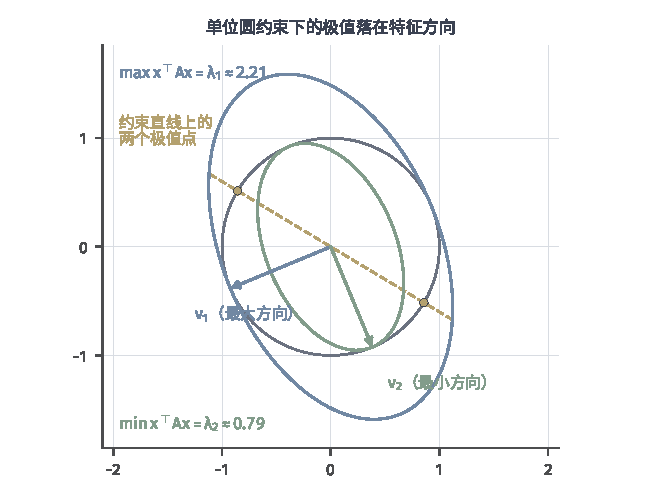
\includegraphics[width=112mm]{figures/00-shared/mathematical-preliminaries-upper/02-linear-spaces/matplotlib/ls-sphere-constrained-extremum/ls-sphere-constrained-extremum.pdf}
  \caption{单位圆约束下的极值落在特征方向。$\bm S=\left[\begin{smallmatrix}2&0.5\\0.5&1\end{smallmatrix}\right]$，
  灰圆为$\lVert\bm x\rVert=1$。蓝椭圆$\bm x^\top\bm S\bm x=\lambda_1\approx2.21$在
  $\pm\bm v_1$处与单位圆相切（最大值），绿椭圆$=\lambda_2\approx0.79$在$\pm\bm v_2$处
  相切（最小值）；黄色虚线为子空间约束直线，其上黄点是该约束下的两个极值。
  $\lambda_{1,2}=(3\pm\sqrt2)/2$。固定复算。}
  \label{fig:ls-sphere-constrained-extremum}
\end{figure}

加权平均介于被平均各数的最小值与最大值之间，由此立即得到两端特征值的极值刻画。
\begin{theorem}[Rayleigh--Ritz]
\label{thm:matrix-analysis-rayleigh-ritz}
\label{eq:matrix-analysis-rayleigh-ritz}
设$\bm S$的特征值为$\lambda_1\geq\cdots\geq\lambda_d$，对应标准正交特征向量$\bm q_1,\ldots,\bm q_d$，则
\begin{equation*}
\begin{gathered}
\max_{\bm x\neq\bm0}R_{\bm S}(\bm x)=\lambda_1\\
\min_{\bm x\neq\bm0}R_{\bm S}(\bm x)=\lambda_d,
\end{gathered}
\end{equation*}
分别在$\bm q_1$与$\bm q_d$取到。
\end{theorem}
\begin{proof}
权重$c_i^2$非负且总和为$1$，所以$\lambda_d\leq\sum_i\lambda_ic_i^2\leq\lambda_1$；取$\bm x=\bm q_1$时只有$c_1=1$，得$\lambda_1$，取$\bm x=\bm q_d$时得$\lambda_d$。
\end{proof}
极值本身唯一，取到极值的方向却未必唯一：$\lambda_1$重复时，其特征空间中每个单位向量都给出最大值；只有在目标特征值单重时，最优方向才唯一（差一个符号）。

\paragraph{齐次最小二乘}
\label{sec:linear-algebra-homogeneous-estimation}

Rayleigh--Ritz定理的一个直接应用是带尺度约束的拟合。有时模型写成$\bm A\bm h\approx\bm0$，只关心$\bm h$各分量之间的比例。这时直接最小化$\lVert\bm A\bm h\rVert_2^2$总会得到平凡解$\bm h=\bm0$，必须先固定尺度。固定$\lVert\bm h\rVert_2=1$后得到的问题称为\term{齐次最小二乘}（homogeneous least squares）：
\begin{equation}
 \min_{\lVert\bm h\rVert_2=1}\ \lVert\bm A\bm h\rVert_2^2
 =\min_{\lVert\bm h\rVert_2=1}\bm h^\top\bm A^\top\bm A\bm h.
 \label{eq:linear-algebra-homogeneous-least-squares}
\end{equation}
右端是对称矩阵$\bm A^\top\bm A$的二次型在单位球面上的最小值。由Rayleigh--Ritz定理，最小值是$\bm A^\top\bm A$的最小特征值，最优$\bm h$是对应的单位特征向量。若$\bm A$有非零零空间，最小值为零，任一单位零空间向量都是最优解。下面的例子属于这种情形。
\begin{example}[一个方程的齐次最小二乘]
\label{ex:ls-homogeneous-least-squares-one-row}
给定一行矩阵$\bm A=[\,1\ -2\,]$。

按式~\eqref{eq:linear-algebra-homogeneous-least-squares}，最优解是$\bm A^\top\bm A$最小特征值的单位特征向量。计算得
\[
 \begin{aligned}
 \bm A^\top\bm A&=\begin{bmatrix}1&-2\\-2&4\end{bmatrix},\\
 \bm A^\top\bm A\,(2,1)^\top&=\bm0,\qquad
 \bm A^\top\bm A\,(1,-2)^\top=5\,(1,-2)^\top .
 \end{aligned}
\]
所以$\bm A^\top\bm A$的特征值为$0$与$5$。

最小特征值$0$对应的单位特征向量为$\bm h=\pm(2,1)^\top/\sqrt5$，它满足$\bm A\bm h=h_1-2h_2=0$。

结论：最小值为$0$，最优解为$\bm h=\pm(2,1)^\top/\sqrt5$；两个符号给出同一个比例$h_1:h_2=2:1$。
\end{example}

\paragraph{Courant--Fischer最小最大原理}

Rayleigh--Ritz定理只刻画两端的特征值。中间的$\lambda_k$不再是整个空间上的极值，但可以借助子空间刻画：在$k$维子空间上取Rayleigh商的最小值，再让子空间变动，取这些最小值中的最大者。

\begin{theorem}[Courant--Fischer]
\label{thm:matrix-analysis-courant-fischer}
\label{eq:matrix-analysis-courant-fischer}
对$k=1,\ldots,d$，
\begin{equation*}
 \lambda_k=\max_{\dim\mathcal V=k}\ \min_{\bm x\in\mathcal V,\bm x\neq\bm0}R_{\bm S}(\bm x)
 =\min_{\dim\mathcal W=d-k+1}\ \max_{\bm x\in\mathcal W,\bm x\neq\bm0}R_{\bm S}(\bm x).
\end{equation*}
\end{theorem}
\begin{proof}
先证第一式。取$\mathcal V_k=\operatorname{span}\{\bm q_1,\dots,\bm q_k\}$，其中单位向量的Rayleigh商是$\lambda_1,\ldots,\lambda_k$的加权平均，不小于$\lambda_k$，所以左端的最大值至少为$\lambda_k$。反过来，任取$k$维子空间$\mathcal V$，令$\mathcal W_k=\operatorname{span}\{\bm q_k,\dots,\bm q_d\}$，它是$d-k+1$维的。由维数公式，
\[
 \dim(\mathcal V\cap\mathcal W_k)\geq\dim\mathcal V+\dim\mathcal W_k-d=1,
\]
所以$\mathcal V$中有非零向量$\bm x$落在$\mathcal W_k$里。它的Rayleigh商是$\lambda_k,\ldots,\lambda_d$的加权平均，不大于$\lambda_k$，因此$\mathcal V$上Rayleigh商的最小值不超过$\lambda_k$。两方面合起来即得第一式。

第二式交换两组特征向量的角色：$\mathcal W_k$上Rayleigh商的最大值恰为$\lambda_k$；任意$d-k+1$维子空间都与$\mathcal V_k$有非零公共向量，其Rayleigh商不小于$\lambda_k$。
\end{proof}
定理只涉及子空间与Rayleigh商，不要求先知道特征向量；第~\ref{sec:ls-spectral-value-sensitivity}节正是用它比较扰动前后的特征值。同样的加权平均论证还可以一次处理$k$个方向，得到前$k$个与后$k$个特征值之和的极值刻画。

\begin{theorem}[迹极值]
\label{thm:matrix-analysis-trace-minimum}
对列标准正交的$\bm V\in\mathbb R^{d\times k}$，
\begin{equation}
 \sum_{i=d-k+1}^{d}\lambda_i\leq\operatorname{tr}(\bm V^\top\bm S\bm V)\leq\sum_{i=1}^{k}\lambda_i,
 \label{eq:matrix-analysis-trace-minimum}
\end{equation}
下界由后$k$个特征向量张成的子空间取到，上界由前$k$个特征向量张成的子空间取到。
\end{theorem}
\begin{proof}
代入$\bm S=\sum_i\lambda_i\bm q_i\bm q_i^\top$，得$\operatorname{tr}(\bm V^\top\bm S\bm V)=\sum_i\lambda_iw_i$，其中$w_i=\lVert\bm V^\top\bm q_i\rVert_2^2$。由$\bm V^\top\bm V=\bm I$得$\lVert\bm V^\top\rVert_2=1$，所以$0\leq w_i\leq1$；又$\sum_iw_i=\lVert\bm V^\top\bm Q\rVert_{\mathrm F}^2=\lVert\bm V\rVert_{\mathrm F}^2=k$。在这两个约束下，
\[
 \begin{aligned}
 \sum_i\lambda_iw_i-\sum_{i\leq k}\lambda_i
 &=\sum_{i\leq k}\lambda_i(w_i-1)+\sum_{i>k}\lambda_iw_i\\
 &\leq\lambda_k\sum_{i\leq k}(w_i-1)+\lambda_k\sum_{i>k}w_i
 =\lambda_k\Bigl(\sum_iw_i-k\Bigr)=0,
 \end{aligned}
\]
其中不等号用到$w_i-1\leq0$、$\lambda_i\geq\lambda_k$（$i\leq k$）与$w_i\geq0$、$\lambda_i\leq\lambda_k$（$i>k$）。这就是上界；对$-\bm S$应用上界即得下界。$\bm V$取前$k$个或后$k$个特征向量时，等号成立。
\end{proof}
上界说明，用$k$维子空间保留二次型的“能量”，最好的选择是前$k$个特征方向，这是主成分分析的代数基础。

\paragraph{广义特征问题}

有时长度不按欧氏范数度量，而按第~\ref{sec:ls-weighted-inner-products}节的加权内积度量，约束$\lVert\bm x\rVert_2=1$相应地换成$\bm x^\top\bm B\bm x=1$（$\bm B\succ0$），要比较的是广义Rayleigh商$\bm x^\top\bm S\bm x/\bm x^\top\bm B\bm x$。它可以化回普通情形。由定理~\ref{thm:ls-gram-factor}写$\bm B=\bm L^\top\bm L$，$\bm L$可逆，令$\bm z=\bm L\bm x$，则$\bm x^\top\bm B\bm x=\bm z^\top\bm z$，而
\[
 \frac{\bm x^\top\bm S\bm x}{\bm x^\top\bm B\bm x}
 =\frac{\bm z^\top\bm L^{-\top}\bm S\bm L^{-1}\bm z}{\bm z^\top\bm z}
\]
是对称矩阵$\bm L^{-\top}\bm S\bm L^{-1}$的普通Rayleigh商。其特征方程$\bm L^{-\top}\bm S\bm L^{-1}\bm z=\mu\bm z$左乘$\bm L^\top$并换回$\bm v=\bm L^{-1}\bm z$，就是下面的方程。
\begin{definition}[广义特征值]
\label{def:matrix-analysis-generalized-eigenvalue}
对实对称$\bm S$与$\bm B\succ0$，称满足
\begin{equation}
\begin{gathered}
\bm S\bm v=\mu\bm B\bm v\\
\bm v\neq\bm0
\end{gathered}
\label{eq:matrix-analysis-generalized-eigenproblem}
\end{equation}
的$\mu$为广义特征值，$\bm v$为广义特征向量，求解它们的问题称为\term{广义特征问题}（generalized eigenvalue problem）。
\end{definition}
对$\bm L^{-\top}\bm S\bm L^{-1}$应用谱定理可知：广义特征值全为实数；广义特征向量可以取为$\bm B$正交的，即$\bm v_i^\top\bm B\bm v_j=\delta_{i,j}$（因为$\bm z_i=\bm L\bm v_i$标准正交）；最大、最小广义特征值就是广义Rayleigh商的最大、最小值。

计算时也应走这条换元的路。直接对$\bm B^{-1}\bm S$求特征值虽然得到同样的$\mu$，但$\bm B^{-1}\bm S$一般不对称，会丢掉对称结构带来的正交性与数值稳定性。

\subsection{由谱定义对称矩阵的函数}
\label{sec:ls-matrix-functions}
\label{sec:matrix-analysis-functions-structured-operations}

多项式$p(\bm S)$可以直接用矩阵的幂与加法算出。平方根、对数、指数这类非多项式函数怎样作用于矩阵？谱定理提示了做法。由$\bm S=\bm Q\bm\Lambda\bm Q^\top$与$\bm Q^\top\bm Q=\bm I$，连乘时相邻的$\bm Q^\top\bm Q$相消，得$\bm S^k=\bm Q\bm\Lambda^k\bm Q^\top$；再按系数相加，得$p(\bm S)=\bm Q\,p(\bm\Lambda)\,\bm Q^\top$。也就是说，多项式在每个特征方向上只作用于对应的特征值。把这一观察作为定义，推广到一般函数。

\paragraph{沿特征方向的定义}

设$\bm S=\bm Q\bm\Lambda\bm Q^\top$，$f$是定义在全部特征值$\lambda_i$上的实函数，令
\begin{equation}
 f(\bm S)=\bm Q\operatorname{diag}\bigl(f(\lambda_1),\ldots,f(\lambda_d)\bigr)\bm Q^\top.
 \label{eq:ls-symmetric-spectral-function}
\end{equation}
$\bm Q$不唯一，需要检查结果是否依赖它的选取。把同一特征值$\lambda$的特征向量归为一组，$\sum_{\lambda_i=\lambda}\bm q_i\bm q_i^\top$是到特征空间$\ker(\bm S-\lambda\bm I)$的正交投影$\bm P_\lambda$，它只依赖这个子空间，与子空间内基的选取无关。于是$f(\bm S)=\sum_\lambda f(\lambda)\bm P_\lambda$，求和遍历不同的特征值，结果由$\bm S$唯一确定。$f(z)=z^k$时，定义回到矩阵幂$\bm S^k$，与已有运算相容。

矩阵函数作用在特征方向上，而不是逐元素作用。下面的例子对照这两种做法。
\begin{example}[矩阵平方根与逐元素开方]
\label{ex:ls-matrix-square-root-two-by-two}
给定示例~\ref{ex:ls-symmetric-spectral-two-by-two}的$\bm S=3\bm q_1\bm q_1^\top+\bm q_2\bm q_2^\top$，取$f(z)=\sqrt z$。按式~\eqref{eq:ls-symmetric-spectral-function}，
\[
 f(\bm S)=\sqrt3\,\bm q_1\bm q_1^\top+\bm q_2\bm q_2^\top
 =\frac12\begin{bmatrix}\sqrt3+1&\sqrt3-1\\\sqrt3-1&\sqrt3+1\end{bmatrix}.
\]
它的平方为
\[
 \frac14\begin{bmatrix}(\sqrt3+1)^2+(\sqrt3-1)^2&2(\sqrt3+1)(\sqrt3-1)\\2(\sqrt3+1)(\sqrt3-1)&(\sqrt3+1)^2+(\sqrt3-1)^2\end{bmatrix}
 =\frac14\begin{bmatrix}8&4\\4&8\end{bmatrix}=\bm S .
\]
逐元素开方得到$\left[\begin{smallmatrix}\sqrt2&1\\1&\sqrt2\end{smallmatrix}\right]$，它的平方是$\left[\begin{smallmatrix}3&2\sqrt2\\2\sqrt2&3\end{smallmatrix}\right]\neq\bm S$。结论：沿特征方向定义的$f(\bm S)$满足$f(\bm S)^2=\bm S$，逐元素开方的结果则不满足。
\end{example}

\paragraph{平方根、实幂与对数}

$\bm S$半正定时，全部$\lambda_i\geq0$，可取$f(z)=\sqrt z$，得到\term{矩阵平方根}（matrix square root）
\[
 \bm S^{1/2}=\bm Q\operatorname{diag}(\sqrt{\lambda_1},\ldots,\sqrt{\lambda_d})\bm Q^\top ,
\]
它半正定且$(\bm S^{1/2})^2=\bm S$。

方程$\bm X^2=\bm S$一般有多个解，例如$\bm I$与$-\bm I$的平方都是$\bm I$；但要求$\bm X$半正定后，解是唯一的。

设半正定的$\bm X=\sum_j\mu_j\bm p_j\bm p_j^\top$（$\mu_j\geq0$，$\bm p_j$标准正交）满足$\bm X^2=\bm S$，则$\bm S=\sum_j\mu_j^2\bm p_j\bm p_j^\top$，即每个$\bm p_j$都是$\bm S$的特征向量，特征值为$\mu_j^2$。于是$\bm S$的$\lambda$特征空间恰由满足$\mu_j^2=\lambda$的那些$\bm p_j$张成，而$\mu_j\geq0$迫使这些$\mu_j=\sqrt\lambda$。所以$\bm X$在$\bm S$的每个特征空间上都乘以$\sqrt\lambda$，这正是$\bm S^{1/2}$的作用，$\bm X=\bm S^{1/2}$。

$\bm S$正定时，全部$\lambda_i>0$，还可以取任意实幂$\bm S^\alpha$，例如$\alpha=-1/2$给出逆平方根；也可以取\term{矩阵对数}（matrix logarithm）：
\[
 \log\bm S=\bm Q\operatorname{diag}(\log\lambda_1,\ldots,\log\lambda_d)\bm Q^\top.
\]
有零特征值时，负幂与对数都没有定义。注意$\log\bm S$是矩阵，而$\log\det\bm S=\sum_i\log\lambda_i=\operatorname{tr}(\log\bm S)$是标量，二者不能混淆。

按定义计算需要完整的谱分解，代价较高。若只需计算$\lVert\bm S^{1/2}\bm x\rVert_2$或作用$\bm S^{-1/2}$做白化，可以用定理~\ref{thm:ls-gram-factor}的因子代替平方根：写$\bm S=\bm L^\top\bm L$，则$\lVert\bm L\bm x\rVert_2^2=\bm x^\top\bm S\bm x=\lVert\bm S^{1/2}\bm x\rVert_2^2$，两者给出同样的长度。第~\ref{chap:linear-equations-and-optimization}章的Cholesky分解把$\bm L$取成三角矩阵，那时作用$\bm L^{-1}$只需解三角方程。

至此，本节的问题有了回答。能用正交矩阵对角化的实矩阵，即具有一组标准正交特征向量的实矩阵，恰好是对称矩阵；谱分解$\bm S=\bm Q\bm\Lambda\bm Q^\top$把它写成沿互相垂直方向的伸缩。特征值同时是Rayleigh商的极值与最小最大值，可以只凭二次型来比较；矩阵函数沿特征方向逐个作用于特征值。但许多重要的方阵并不对称，例如平面旋转与示例~\ref{ex:ls-triangular-power}的上三角矩阵$\left[\begin{smallmatrix}0.8&4\\0&0.5\end{smallmatrix}\right]$。下一节讨论，对一般方阵，坚持用正交矩阵换基时最多能化到多简单。

% 第6章第4节：一般方阵的对角化（复特征值与谱半径、实Schur形与正规矩阵）。

\section{一般方阵的Schur形}
\label{sec:ls-general-square-spectrum}

前两节的对角化各有前提：用可逆矩阵对角化，要求有足够多的实特征向量；用正交矩阵对角化，要求矩阵对称。不对称的方阵会在两处偏离这些前提。其一，实特征值可能不够：平面上的$90^\circ$旋转没有实特征向量，第~\ref{sec:ls-matrix-powers}节的对角化在第一步就停止。其二，即使可以对角化，特征向量也可能互不正交：示例~\ref{ex:ls-triangular-power}中矩阵的两条特征方向$(1,0)^\top$与$(-40/3,1)^\top$夹角只有约$4.3^\circ$（计算见示例~\ref{ex:ls-nonnormal-norm-radius}）。本节回答三个问题：非实的特征值在实空间中对应什么作用，怎样用一个数概括矩阵每作用一次的伸缩倍数；若坚持用正交矩阵换基，一般方阵最多能化到多接近对角的形式；什么样的方阵在这种换基下仍能化为分块对角形。

\subsection{复特征值与实不变平面}

第~\ref{sec:ls-characteristic-polynomial}节的特征多项式$p_{\bm A}$是$d$次实系数多项式。由代数基本定理，它在复数范围内恰有$d$个根（计重数）。把这些根都称为$\bm A$的特征值，全体特征值组成的集合称为$\bm A$的\term{谱}（spectrum）。由于系数都是实数，若$p_{\bm A}(\lambda)=0$，两边取共轭即得$p_{\bm A}(\bar\lambda)=0$，所以非实根成共轭对出现。实特征值的情形与第~\ref{sec:ls-linear-operators}节相同。

第~\ref{sec:ls-eigen-similarity-invariance}节由系数比较得到$\operatorname{tr}\bm A=\sum_i\lambda_i$与$\det\bm A=\prod_i\lambda_i$，那里要求$p_{\bm A}$能分解为实一次因子。计入复特征值以后，$p_{\bm A}$在复数范围内总能分解为一次因子之积，同样的系数比较说明，这两个等式对每个方阵都成立。

非实特征值在实空间里对应什么作用？设$\lambda=a+\mathrm ib$（$b\neq0$）是特征值。复矩阵$\bm A-\lambda\bm I$的行列式为零，所以有非零的复向量$\bm u+\mathrm i\bm w$满足$\bm A(\bm u+\mathrm i\bm w)=(a+\mathrm ib)(\bm u+\mathrm i\bm w)$，其中$\bm u,\bm w$为实向量。比较两边的实部与虚部，得
\[
 \begin{gathered}
\bm A\bm u=a\bm u-b\bm w\\
\bm A\bm w=b\bm u+a\bm w .
 \end{gathered}
\]

这两个等式说明$\operatorname{span}\{\bm u,\bm w\}$在$\bm A$下不变。它是二维的，即$\bm u,\bm w$线性无关。否则$\bm u,\bm w$（不全为零）只张成一条直线$\operatorname{span}\{\bm y\}$，这条直线在$\bm A$下不变，所以$\bm A\bm y=\mu\bm y$，$\mu$为实数；而$\bm u+\mathrm i\bm w$是$\bm y$的复数倍，于是$\bm A(\bm u+\mathrm i\bm w)=\mu(\bm u+\mathrm i\bm w)$，得$\lambda=\mu$为实数，与$b\neq0$矛盾。所以$\operatorname{span}\{\bm u,\bm w\}$是二维实不变子空间。在基$(\bm u,\bm w)$下，$\bm A$的作用由矩阵
\[
\begin{gathered}
\begin{bmatrix}a&b\\-b&a\end{bmatrix}
 =|\lambda|\begin{bmatrix}\cos\phi&\sin\phi\\-\sin\phi&\cos\phi\end{bmatrix}\\
\cos\phi=\frac{a}{|\lambda|},\ \sin\phi=\frac{b}{|\lambda|}
\end{gathered}
\]
表示。在这组坐标中，它是$|\lambda|$倍的伸缩加一次旋转。基$(\bm u,\bm w)$一般不是标准正交基，因此这个坐标描述不能直接当作原空间中欧氏长度和角度的变化。

因此特征值的模长$|\lambda|$描述特征方向或上述平面坐标中每次作用的倍率；它一般不是矩阵在欧氏范数下的一步最大放大倍数。全部特征值模长的最大值
\[
 \rho(\bm A)=\max_i|\lambda_i(\bm A)|
\]
称为\term{谱半径}（spectral radius）。例如$90^\circ$旋转的特征值为$\pm\mathrm i$，谱半径为$1$：它不改变长度，只改变方向。

\subsection{实Schur分解}

\paragraph{实Schur形}

一般方阵未必能对角化，更未必能用正交矩阵对角化。退一步，能否用正交矩阵把它化为上三角形？上三角形同样便于计算：对角元就是特征值，解方程和求幂都可以从最后一个坐标逐个向前推。实特征值不够时，实上三角形不可能存在，因为它的对角元就是特征值，必须全是实数；但允许对角线上出现$2\times2$块以后，答案总是肯定的。

\begin{theorem}[实Schur形]
\label{thm:ls-real-schur}
对任意$\bm A\in\mathbb R^{d\times d}$，存在正交矩阵$\bm Q$与分块上三角矩阵$\bm T$，使
\begin{equation}
 \bm A=\bm Q\bm T\bm Q^{\top},
 \label{eq:matrix-analysis-schur-decomposition}
\end{equation}
$\bm T$的对角块为$1\times1$（实特征值）或$2\times2$（一对共轭特征值），对角块下方全为零。$\bm A$的特征值就是各对角块的特征值。
\end{theorem}
\begin{proof}
对$d$归纳：先找一个不变子空间，再把矩阵写成分块上三角形式，对右下角的压缩矩阵降维。这里一般不能假定该不变子空间的正交补也不变。若$\bm A$有实特征值$\lambda$，取单位特征向量$\bm q_1$并扩充为正交矩阵$\bm Q_1=[\bm q_1,\bm Q_2]$。由$\bm A\bm q_1=\lambda\bm q_1$与$\bm Q_2^\top\bm q_1=\bm0$，$\bm Q_1^\top\bm A\bm Q_1$的第一列为$\lambda\bm e_1$，即
\[
 \bm Q_1^\top\bm A\bm Q_1=\begin{bmatrix}\lambda&*\\\bm0&\bm Q_2^\top\bm A\bm Q_2\end{bmatrix}.
\]
若没有实特征值，取上一小节得到的二维不变子空间，用它的一组标准正交基$\bm q_1,\bm q_2$同样扩充，得到左上角为$2\times2$块、其下方为零的分块形式，该块的特征值是$\lambda,\bar\lambda$。分块上三角矩阵的特征多项式是对角块特征多项式之积，所以右下块的特征值恰为其余特征值。对右下块应用归纳假设，再把两次正交变换合并，即得结论。
\end{proof}
实际计算先用Householder反射化为上Hessenberg形，再作带位移的QR迭代，标准数值软件都提供这一分解；本卷只使用它的存在性。第~\ref{sec:ls-sylvester-schur}节求解Sylvester方程时，用的正是这一形式。

\subsection{正规矩阵与非正规矩阵}

Schur形什么时候是分块对角的？实对称矩阵是一例。这时$\bm T=\bm Q^\top\bm A\bm Q$仍对称，它的$2\times2$对角块也对称，特征值为实数，不可能对应一对共轭特征值，所以$\bm T$只有$1\times1$对角块，是上三角矩阵；对称的上三角矩阵只能是对角矩阵，这又一次得到谱定理。
更一般地，第~\ref{sec:ls-adjoints}节把满足$TT^\star=T^\star T$的算子称为正规算子。在标准坐标下伴随就是转置，满足$\bm A^\top\bm A=\bm A\bm A^\top$的矩阵称为\term{正规矩阵}（normal matrix）；对称、反对称与正交矩阵都是正规的。

正规矩阵的Schur形$\bm T$分块对角。首先$\bm T$也正规：$\bm T^\top\bm T=\bm Q^\top\bm A^\top\bm A\bm Q=\bm Q^\top\bm A\bm A^\top\bm Q=\bm T\bm T^\top$。比较$\bm T^\top\bm T$与$\bm T\bm T^\top$的左上角对角块：前者是$\bm T_{1,1}^\top\bm T_{1,1}$，因为$\bm T$的第一块列只有$\bm T_{1,1}$非零；后者是$\sum_j\bm T_{1,j}\bm T_{1,j}^\top$。两边取迹，得
\[
 \lVert\bm T_{1,1}\rVert_{\mathrm F}^2=\lVert\bm T_{1,1}\rVert_{\mathrm F}^2+\sum_{j>1}\lVert\bm T_{1,j}\rVert_{\mathrm F}^2 ,
\]
故第一块行的非对角块全为零。去掉第一块后，剩下的矩阵仍正规，逐块推下去可知$\bm T$分块对角。

每个$2\times2$对角块$\left[\begin{smallmatrix}p&q\\r&s\end{smallmatrix}\right]$也正规。比较两边的$(1,1)$元得$q^2=r^2$。若$q=r$，块对称，特征值为实数，与$2\times2$块对应一对共轭特征值矛盾；所以$r=-q\neq0$。再比较$(1,2)$元得$2q(s-p)=0$，即$s=p$。于是每块都形如$\left[\begin{smallmatrix}a&b\\-b&a\end{smallmatrix}\right]$，是模长乘旋转。反过来，若正交矩阵$\bm Q$把$\bm A$化为分块对角矩阵$\bm T$，且每块是一个数或这种模长乘旋转的块，则每块与自己的转置可交换，$\bm T^\top\bm T=\bm T\bm T^\top$，从而$\bm A=\bm Q\bm T\bm Q^\top$正规。所以正规矩阵恰好是能用标准正交基化为这种分块对角形的实方阵。

总之，正规矩阵沿一组标准正交的方向或平面只作伸缩，或伸缩加旋转。$\bm T^k$仍分块对角，每块是$\lambda^k$或$|\lambda|^k$乘一个旋转，二范数为$|\lambda|^k$；正交变换又不改变谱范数，所以$\lVert\bm A^k\rVert_2=\lVert\bm T^k\rVert_2=\max_i|\lambda_i|^k=\rho(\bm A)^k$。也就是说，正规矩阵每一步的最大放大倍数恰好就是谱半径。

\paragraph{非正规矩阵}
由上一段，非正规矩阵的Schur形$\bm T$不可能是由数与模长乘旋转块组成的分块对角形：它要么含非零的非对角块，要么某个$2\times2$对角块本身不正规。非正规矩阵也不能用一组标准正交的特征向量对角化，否则它对称。这时矩阵范数可以远大于谱半径，下面的例子显示了这种分离。
\begin{example}[非正规矩阵的范数与谱半径]
\label{ex:ls-nonnormal-norm-radius}
给定示例~\ref{ex:ls-triangular-power}的$\bm A=\left[\begin{smallmatrix}0.8&4\\0&0.5\end{smallmatrix}\right]$，比较它的谱半径、一步的放大倍数与特征方向的夹角。

它不正规：$\bm A^\top\bm A$的$(1,1)$元为$0.8^2=0.64$，$\bm A\bm A^\top$的$(1,1)$元为$0.8^2+4^2=16.64$。特征值为$0.8$与$0.5$，所以$\rho(\bm A)=0.8$。一步作用把$(0,1)^\top$送到$(4,0.5)^\top$，长度为$\sqrt{16.25}>4$，所以$\lVert\bm A\rVert_2>4$。两条特征方向$\bm v_1=(1,0)^\top$与$\bm v_2=(-40/3,1)^\top$的夹角$\theta$满足
\[
 \cos\theta=\frac{|\bm v_1^\top\bm v_2|}{\lVert\bm v_1\rVert_2\lVert\bm v_2\rVert_2}
 =\frac{40/3}{\sqrt{(40/3)^2+1}}\approx0.997,
\]
即$\theta\approx4.3^\circ$。结论：两条特征方向几乎平行，一步的最大放大倍数超过$4$，而谱半径只有$0.8$。
\end{example}
谱半径描述反复作用的长期倍率，范数描述一步的最大放大；非正规时二者可以分离。第~\ref{sec:ls-matrix-power-behavior}节将看到，这种分离可能伴随先放大、后衰减的瞬态。

至此，本节的问题有了回答。实矩阵的特征值可能是复数，一对共轭特征值$a\pm\mathrm ib$对应一个二维不变平面，其某组基下的坐标作伸缩加旋转；谱半径$\rho(\bm A)$概括每作用一次的长期伸缩倍数。坚持用标准正交基时，一般方阵只能化为实Schur形；恰好能化为由数与模长乘旋转块组成的分块对角形的是正规矩阵，它每一步的最大放大等于谱半径，非正规矩阵的范数与谱半径则可能相差悬殊。这些结论都要求矩阵把空间映到自身，并且输入、输出用同一组基。若允许两端各取一组标准正交基，这一限制就消失了：下一节说明，任何矩阵都能这样化为对角形。

% 第6章第5节：奇异值分解（构造、奇异值与矩阵范数、极分解、最佳低秩逼近）。

\section{奇异值分解与低秩逼近}
\label{sec:ls-svd}

前面几节都让输入与输出使用同一组基。在这一要求下用标准正交基换基，只有对称矩阵能化为实对角形，正规矩阵能化为分块对角形，一般方阵只能化为分块上三角的实Schur形。矩形矩阵$\bm A\in\mathbb R^{m\times d}$的输入在$\mathbb R^d$中、输出在$\mathbb R^m$中，“同一组基”与特征向量都无从谈起。于是放宽要求：能否在输入端找一组标准正交方向$\bm v_i$，在输出端找一组标准正交方向$\bm u_i$，使
\[
\begin{gathered}
\bm A\bm v_i=\sigma_i\bm u_i\\
\sigma_i\geq0,
\end{gathered}
\]
其中$i$取$1,\ldots,\min(m,d)$。也就是说，$\bm A$把第$i$个输入方向伸缩$\sigma_i$倍后送到第$i$个输出方向；若输入维数更大，多出的输入基向量还须映到零。能否做到这一点？本节先证明这对任意矩阵都可以做到。所需的方向来自对称矩阵$\bm A^\top\bm A$的特征方向，构造只用到谱定理（定理~\ref{thm:ls-real-symmetric-spectral}）。然后说明这种分解给出了什么：谱范数与Frobenius范数的值，把方阵的作用分成伸缩与转动的极分解，以及给定秩上限时最好的近似。

\subsection{奇异值分解的构造}

先看这样的方向若存在，应当是什么。

设$\bm x=\sum_ic_i\bm v_i$，则$\bm A\bm x=\sum_ic_i\sigma_i\bm u_i$，由$\bm u_i$标准正交，
\[
 \bm x^\top\bm A^\top\bm A\bm x=\lVert\bm A\bm x\rVert_2^2=\sum_i\sigma_i^2c_i^2 .
\]
与二次型展开式~\eqref{eq:matrix-analysis-quadratic-spectral-form}比较可知，$\bm v_i$应是对称矩阵$\bm A^\top\bm A$的特征向量，$\sigma_i^2$是对应的特征值。这提示从$\bm A^\top\bm A$出发构造。

令$\bm S=\bm A^\top\bm A$。它对称，而且半正定：$\bm x^\top\bm A^\top\bm A\bm x=\lVert\bm A\bm x\rVert_2^2\geq0$。由谱定理，存在$\mathbb R^d$的标准正交基$\bm v_1,\ldots,\bm v_d$使$\bm A^\top\bm A\bm v_i=\lambda_i\bm v_i$，且$\lambda_1\geq\cdots\geq\lambda_d\geq0$。设前$r$个特征值为正，记$\sigma_i=\sqrt{\lambda_i}>0$（$i\leq r$）。其余的$\bm v_j$满足$\lVert\bm A\bm v_j\rVert_2^2=\bm v_j^\top\bm A^\top\bm A\bm v_j=0$，即$\bm A\bm v_j=\bm0$。

对$i\leq r$定义输出方向$\bm u_i=\bm A\bm v_i/\sigma_i$。它们标准正交：
\[
 \bm u_i^\top\bm u_j
 =\frac{\bm v_i^\top\bm A^\top\bm A\bm v_j}{\sigma_i\sigma_j}
 =\frac{\sigma_j^2\,\bm v_i^\top\bm v_j}{\sigma_i\sigma_j}=\delta_{i,j}.
\]
再把$\bm u_1,\dots,\bm u_r$扩充为$\mathbb R^m$的标准正交基$\bm u_1,\ldots,\bm u_m$。

现在把任意$\bm x$展开为$\bm x=\sum_i(\bm v_i^\top\bm x)\bm v_i$，再利用$\bm A\bm v_i=\sigma_i\bm u_i$（$i\leq r$）与$\bm A\bm v_j=\bm0$（$j>r$），得
\[
 \bm A\bm x=\sum_{i=1}^r\sigma_i\bm u_i(\bm v_i^\top\bm x).
\]
这对所有$\bm x$成立，所以$\bm A$是$r$个秩一矩阵之和：
\begin{equation}
 \bm A=\sum_{i=1}^r\sigma_i\bm u_i\bm v_i^\top.
 \label{eq:matrix-analysis-svd-rank-one-sum}
\end{equation}
由这个和式，$\operatorname{range}(\bm A)$由$\bm u_1,\ldots,\bm u_r$张成；又因为$\bm u_i$线性无关且$\sigma_i>0$，$\bm A\bm x=\bm0$当且仅当$\bm v_i^\top\bm x=0$（$i\leq r$），所以$\ker\bm A$由$\bm v_{r+1},\ldots,\bm v_d$张成。于是$r=\operatorname{rank}\bm A$。把这些向量排成矩阵，就得到下面的结论。

\begin{theorem}[SVD的存在]
\label{thm:ls-svd-existence}
对任意$\bm A\in\mathbb R^{m\times d}$，存在正交矩阵$\bm U\in\mathbb R^{m\times m}$、$\bm V\in\mathbb R^{d\times d}$与对角矩阵$\bm\Sigma\in\mathbb R^{m\times d}$，使$\bm A=\bm U\bm\Sigma\bm V^\top$；$\bm\Sigma$的对角元$\sigma_1\geq\cdots\geq\sigma_{\min(m,d)}\geq0$，其中恰有$\operatorname{rank}\bm A$个为正。
\end{theorem}

\begin{definition}[奇异值分解]
\label{def:matrix-analysis-svd}
称
\begin{equation}
 \bm A=\bm U\bm\Sigma\bm V^\top
 \label{eq:matrix-analysis-svd}
\end{equation}
为$\bm A$的\term{奇异值分解}（singular value decomposition, SVD），$\bm\Sigma$的对角元$\sigma_i$称为\term{奇异值}（singular value），$\bm U$、$\bm V$的列$\bm u_i$、$\bm v_i$分别称为左、右\term{奇异向量}（singular vector）。
\end{definition}

图~\ref{fig:ls-svd-construction}把构造拆成三步：形成$\bm A^\top\bm A$；由谱定理将其对角化；开方得到奇异值，再由$\bm u_i=\bm A\bm v_i/\sigma_i$得到左奇异向量。

\begin{figure*}[htbp]
  \centering
  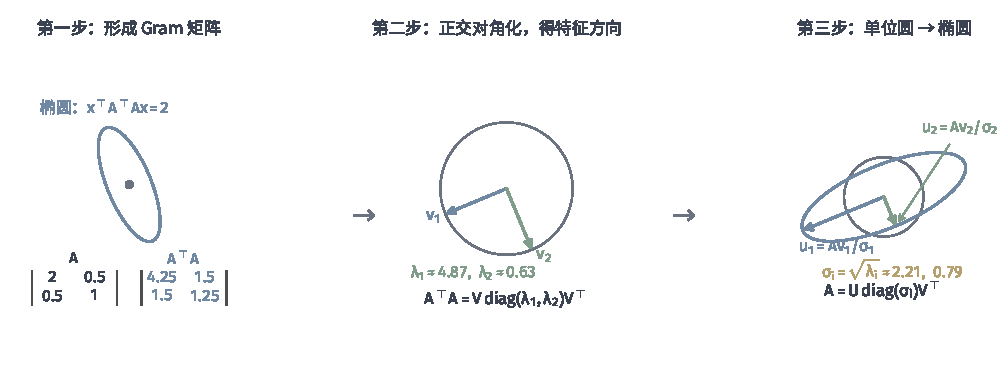
\includegraphics[width=168.998mm]{figures/00-shared/mathematical-preliminaries-upper/02-linear-spaces/matplotlib/ls-svd-construction/ls-svd-construction.pdf}
  \caption{SVD 构造三部曲。以$\bm A=\left[\begin{smallmatrix}2&0.5\\0.5&1\end{smallmatrix}\right]$为例：
  (1)形成$\bm A^\top\bm A=\left[\begin{smallmatrix}4.25&1.5\\1.5&1.25\end{smallmatrix}\right]$；
  (2)由谱定理对角化，特征值$\lambda_1\approx4.87,\lambda_2\approx0.63$；
  (3)$\sigma_i=\sqrt{\lambda_i}\approx2.21,0.79$，右奇异向量$\bm v_i$即特征向量，
  左奇异向量$\bm u_i=\bm A\bm v_i/\sigma_i$。解析式教学构造。}
  \label{fig:ls-svd-construction}
\end{figure*}

几何上，$\bm A$把输入端的单位球映成输出空间中一个椭球（秩亏时它落在低维子空间内）：$\bm v_i$方向的单位向量被送到长度为$\sigma_i$的半轴$\sigma_i\bm u_i$。若输入空间存在非零零空间，单位球面上的点也可能映到这个椭球的内部，因此这里以单位球而非球面描述整个像。图~\ref{fig:matrix-analysis-svd-geometry}用二维旋转矩阵$\bm R(\theta)=\left[\begin{smallmatrix}\cos\theta&-\sin\theta\\\sin\theta&\cos\theta\end{smallmatrix}\right]$构造了一个输入方向与输出方向不同的例子。

\begin{figure*}[htbp]
  \centering
  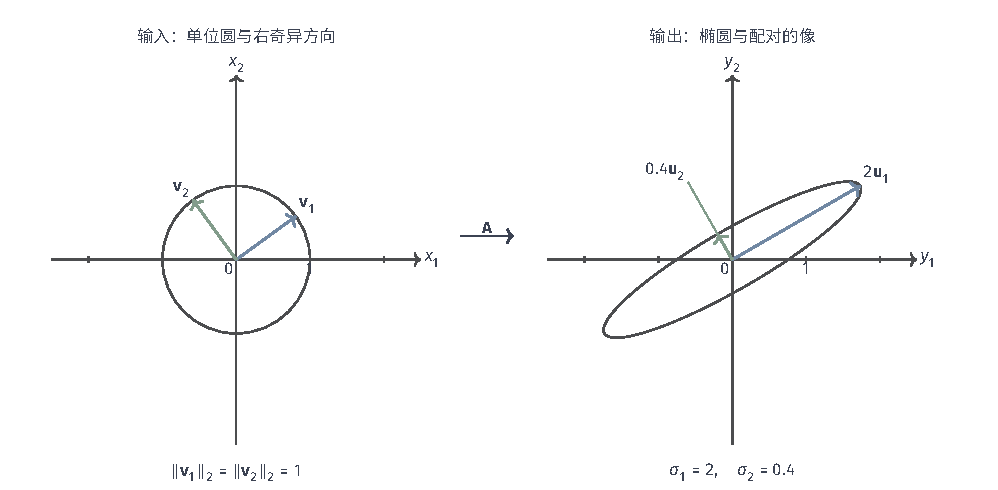
\includegraphics[width=168.998mm]{figures/00-shared/mathematical-preliminaries-upper/02-linear-spaces/tikz/matrix-analysis-svd-geometry/figure.pdf}
  \caption{矩阵$\bm A=\bm R(\pi/6)\operatorname{diag}(2,0.4)\bm R(\pi/5)^\top$
  将单位圆变为椭圆。蓝、绿分别对应两个奇异方向；同色箭头在左侧标出$\bm v_i$，
  在右侧标出其像$\sigma_i\bm u_i$。两侧坐标比例相同。奇异值决定长度变化，左右方向可以不同，
  因而这不是沿特征方向的同空间缩放。图为教学构造。}
  \label{fig:matrix-analysis-svd-geometry}
\end{figure*}

奇异值由$\bm A$唯一确定，它们是$\bm A^\top\bm A$特征值的平方根。
奇异向量则不唯一：正奇异值重复时，可以在对应的右奇异子空间内另选标准正交基，再由$\bm u_i=\bm A\bm v_i/\sigma_i$确定配对的左奇异向量；一对$\bm u_i,\bm v_i$也可以同时变号。

构造虽然从$\bm A^\top\bm A$出发，数值计算却通常不直接形成它：$\bm A^\top\bm A$的特征值是$\sigma_i^2$，小奇异值平方后更小，在舍入中最先失去精度，第~\ref{chap:linear-equations-and-optimization}章讨论最小二乘的数值敏感性时会具体看到这一点。标准算法直接对$\bm A$从两侧施加正交变换，把它化为上双对角形，再迭代求出奇异值；只需要前几个奇异方向时，可以只计算相应的部分。

\subsection{奇异值与矩阵的大小}

第~\ref{sec:ls-frobenius-norm}节与第~\ref{sec:ls-matrix-norms}节分别定义了Frobenius范数与谱范数，但没有给出谱范数的算法。SVD直接给出两者的值。对$\bm x=\sum_ic_i\bm v_i$，
\[
 \lVert\bm A\bm x\rVert_2^2=\sum_{i\leq r}\sigma_i^2c_i^2\leq\sigma_1^2\sum_ic_i^2=\sigma_1^2\lVert\bm x\rVert_2^2 ,
\]
等号在$\bm x=\bm v_1$时成立；而$\lVert\bm A\rVert_{\mathrm F}^2=\operatorname{tr}(\bm A^\top\bm A)$等于$\bm A^\top\bm A$的特征值之和$\sum_i\sigma_i^2$。因此
\begin{align}
 \lVert\bm A\rVert_2&=\sigma_1,
 \label{eq:matrix-analysis-spectral-norm}\\
 \lVert\bm A\rVert_{\mathrm F}&=\Bigl(\sum_{i=1}^r\sigma_i^2\Bigr)^{1/2}.
 \label{eq:matrix-analysis-frobenius-norm}
\end{align}
同一展开也给出最弱的放大。$d\leq m$时$\lVert\bm A\bm x\rVert_2\geq\sigma_d\lVert\bm x\rVert_2$，等号在$\bm x=\bm v_d$时成立，秩亏时$\sigma_d=0$。对可逆方阵，$\bm A^{-1}=\sum_i\sigma_i^{-1}\bm v_i\bm u_i^\top$（直接相乘可验证$\bm A\bm A^{-1}=\sum_i\bm u_i\bm u_i^\top=\bm I$），它的最大奇异值是$1/\sigma_d$，所以$\lVert\bm A^{-1}\rVert_2=1/\sigma_d$。

最大奇异值衡量最强的放大，最小奇异值衡量最弱的放大，二者之比就是第~\ref{sec:ls-perturbation-conditioning}节的条件数。齐次最小二乘~\eqref{eq:linear-algebra-homogeneous-least-squares}的最优解也可以由此读出：它是$\bm V$的最后一列$\bm v_d$，因为按构造，$\bm v_d$是$\bm A^\top\bm A$最小特征值的单位特征向量。

\subsection{极分解与正交部分}

SVD还可以把方阵的作用分成“伸缩”与“转动”两步，类似于把复数写成模长与单位复数之积。

设$\bm A\in\mathbb R^{d\times d}$有SVD$\bm A=\bm U\bm\Sigma\bm V^\top$，在$\bm U$与$\bm\Sigma$之间插入$\bm V^\top\bm V=\bm I$，得$\bm A=(\bm U\bm V^\top)(\bm V\bm\Sigma\bm V^\top)$。
\begin{definition}[极分解]
\label{def:matrix-analysis-polar-decomposition}
方阵$\bm A$的\term{极分解}（polar decomposition）是
\begin{equation}
\begin{gathered}
\bm A=\bm W\bm H\\
\bm W=\bm U\bm V^\top,\quad \bm H=\bm V\bm\Sigma\bm V^\top=(\bm A^\top\bm A)^{1/2},
\end{gathered}
\label{eq:matrix-analysis-polar-decomposition}
\end{equation}
其中$\bm W$正交，$\bm H$对称半正定。
\end{definition}
$\bm H$先沿$\bm v_i$方向伸缩，$\bm W$再作正交变换。由$\bm H^2=\bm V\bm\Sigma^2\bm V^\top=\bm A^\top\bm A$及半正定平方根的唯一性，$\bm H$由$\bm A$唯一确定；$\bm A$可逆时$\bm H$可逆，$\bm W=\bm A\bm H^{-1}$也唯一。

正交因子$\bm W$是Frobenius范数下离$\bm A$最近的正交矩阵。对正交$\bm Z$，$\lVert\bm Z\rVert_{\mathrm F}^2=d$，展开得$\lVert\bm A-\bm Z\rVert_{\mathrm F}^2=\lVert\bm A\rVert_{\mathrm F}^2+d-2\operatorname{tr}(\bm Z^\top\bm A)$，所以只需让$\operatorname{tr}(\bm Z^\top\bm A)$最大。由迹的循环性，
\[
 \operatorname{tr}(\bm Z^\top\bm U\bm\Sigma\bm V^\top)=\operatorname{tr}(\bm V^\top\bm Z^\top\bm U\,\bm\Sigma)=\sum_i\sigma_i(\bm V^\top\bm Z^\top\bm U)_{i,i}.
\]
$\bm V^\top\bm Z^\top\bm U$是正交矩阵，其列是单位向量，对角元不超过$1$，故迹不超过$\sum_i\sigma_i$；取$\bm Z=\bm U\bm V^\top$时该矩阵为$\bm I$，等号成立。含噪的旋转估计常用这一步把近似正交的矩阵修正为正交矩阵。

\subsection{截断SVD与最佳低秩逼近}
\label{sec:ls-low-rank-solve}
\label{sec:ls-full-svd-solve}
\label{sec:matrix-analysis-svd-low-rank}

数据矩阵常常近似低秩：少数几个方向承载了大部分信息。给定秩上限$k$，怎样找离$\bm A$最近的秩不超过$k$的矩阵？秩一分解~\eqref{eq:matrix-analysis-svd-rank-one-sum}把$\bm A$按奇异值从大到小拆成$r$项，一个自然的候选是只保留前$k$项。

设$\bm A\in\mathbb R^{m\times d}$的非零奇异值为$\sigma_1\geq\cdots\geq\sigma_r>0$，称
\begin{equation}
\begin{gathered}
\bm A_k=\sum_{i=1}^k\sigma_i\bm u_i\bm v_i^\top\\
0\leq k<r
\end{gathered}
\label{eq:matrix-analysis-truncated-svd}
\end{equation}
为\term{截断SVD}（truncated SVD），$k=0$时$\bm A_0=\bm0$。

余下的$\bm A-\bm A_k=\sum_{i>k}\sigma_i\bm u_i\bm v_i^\top$本身就是一个SVD，最大奇异值为$\sigma_{k+1}$，由式~\eqref{eq:matrix-analysis-spectral-norm}与式~\eqref{eq:matrix-analysis-frobenius-norm}直接读出两种误差：
\begin{equation}
\begin{gathered}
\lVert\bm A-\bm A_k\rVert_2=\sigma_{k+1}\\
\lVert\bm A-\bm A_k\rVert_{\mathrm F}
 =\Bigl(\sum_{i=k+1}^r\sigma_i^2\Bigr)^{1/2}.
\end{gathered}
\label{eq:ls-truncated-errors}
\end{equation}
谱范数误差是最坏单位输入的输出偏差，Frobenius误差累计全部元素的平方偏差。下面的定理说明，在这两种范数下没有比截断SVD更好的秩$k$近似。

\begin{theorem}[Eckart--Young--Mirsky最佳低秩逼近]
\label{thm:ls-best-low-rank}
\label{thm:matrix-analysis-best-low-rank}
对$0\leq k<r=\operatorname{rank}\bm A$，
\begin{align}
 \min_{\operatorname{rank}\bm B\leq k}\lVert\bm A-\bm B\rVert_2
 &=\sigma_{k+1},
 \label{eq:matrix-analysis-best-rank-k-spectral}\\
 \min_{\operatorname{rank}\bm B\leq k}\lVert\bm A-\bm B\rVert_{\mathrm F}
 &=\Bigl(\sum_{i=k+1}^r\sigma_i^2\Bigr)^{1/2},
 \label{eq:matrix-analysis-best-rank-k-frobenius}
\end{align}
两个最小值都由截断SVD$\bm A_k$达到。
\end{theorem}
\begin{proof}
式~\eqref{eq:ls-truncated-errors}说明$\bm A_k$达到右端，只需证明任意秩不超过$k$的$\bm B$误差都不更小。$k=0$时$\bm B=\bm0$，结论即式~\eqref{eq:ls-truncated-errors}，下设$k\geq1$。

谱范数情形。$\ker\bm B$的维数至少为$d-k$，子空间$\operatorname{span}\{\bm v_1,\ldots,\bm v_{k+1}\}$的维数为$k+1$，两者维数之和超过$d$，必有公共单位向量$\bm x=\sum_{i=1}^{k+1}c_i\bm v_i$，$\sum_ic_i^2=1$。由$\bm B\bm x=\bm0$，
\begin{equation}
 \lVert(\bm A-\bm B)\bm x\rVert_2
 =\lVert\bm A\bm x\rVert_2
 =\Bigl(\sum_{i=1}^{k+1}\sigma_i^2c_i^2\Bigr)^{1/2}
 \geq\sigma_{k+1},
 \label{eq:ls-spectral-lower-bound}
\end{equation}
所以$\lVert\bm A-\bm B\rVert_2\geq\sigma_{k+1}$。

Frobenius情形。正交变换不改变Frobenius范数，令$\bm C=\bm U^\top\bm B\bm V$，则$\operatorname{rank}\bm C=\operatorname{rank}\bm B\leq k$，且$\lVert\bm A-\bm B\rVert_{\mathrm F}=\lVert\bm\Sigma-\bm C\rVert_{\mathrm F}$。设$\bm P$为到$\bm C$列空间的正交投影，则$\operatorname{tr}\bm P=\operatorname{rank}\bm C\leq k$，且$\bm P\bm C=\bm C$。把$\bm\Sigma-\bm C$拆成$(\bm I-\bm P)\bm\Sigma$与$\bm P\bm\Sigma-\bm C$，两部分的每一列分别落在互相正交的子空间中，于是
\[
 \lVert\bm\Sigma-\bm C\rVert_{\mathrm F}^2
 =\lVert(\bm I-\bm P)\bm\Sigma\rVert_{\mathrm F}^2+\lVert\bm P\bm\Sigma-\bm C\rVert_{\mathrm F}^2
 \geq\lVert\bm\Sigma\rVert_{\mathrm F}^2-\lVert\bm P\bm\Sigma\rVert_{\mathrm F}^2 .
\]
$\bm\Sigma$的第$i$列是$\sigma_i\bm e_i$，所以保留部分为$\lVert\bm P\bm\Sigma\rVert_{\mathrm F}^2=\sum_i\sigma_i^2w_i$，其中$w_i=\lVert\bm P\bm e_i\rVert_2^2\in[0,1]$，且$\sum_iw_i\leq\lVert\bm P\rVert_{\mathrm F}^2=\operatorname{tr}\bm P\leq k$。与迹极值定理的证明相同，由$\sigma_i$降序，
\[
 \sum_i\sigma_i^2w_i-\sum_{i\leq k}\sigma_i^2
 =\sum_{i\leq k}\sigma_i^2(w_i-1)+\sum_{i>k}\sigma_i^2w_i
 \leq\sigma_k^2\Bigl(\sum_iw_i-k\Bigr)\leq0 .
\]
即保留部分不超过$\sum_{i\leq k}\sigma_i^2$，误差平方至少为$\lVert\bm\Sigma\rVert_{\mathrm F}^2-\sum_{i\leq k}\sigma_i^2=\sum_{i>k}\sigma_i^2$。
\end{proof}
这一结论最早由Eckart与Young给出\scite{eckart1936}。上面的证明只处理谱范数与Frobenius范数；误差改用加权、逐元素或分组的度量时，最优性需要重新论证，截断SVD一般不再是最优解。图~\ref{fig:ls-low-rank-truncation}画出截断的几何：单位圆经$\bm A$变成椭圆，秩一近似把椭圆压成主轴方向的线段，残留误差恰为舍弃的$\sigma_2$。

\begin{figure*}[htbp]
  \centering
  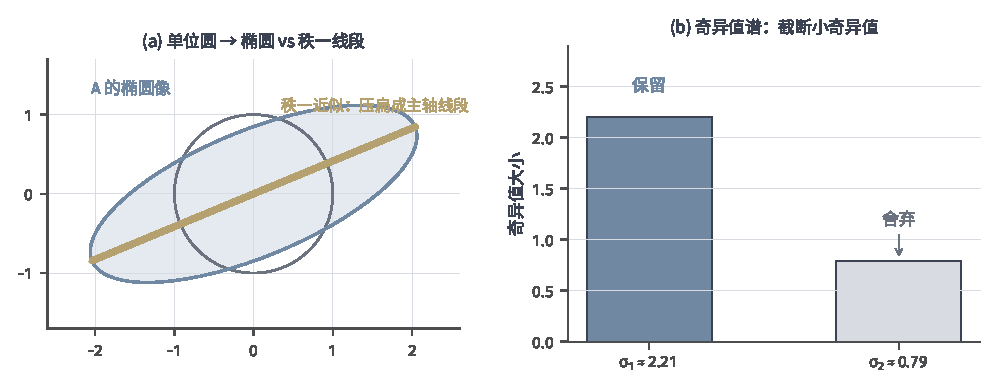
\includegraphics[width=168.998mm]{figures/00-shared/mathematical-preliminaries-upper/02-linear-spaces/matplotlib/ls-low-rank-truncation/ls-low-rank-truncation.pdf}
  \caption{低秩截断的几何。$\bm A=\left[\begin{smallmatrix}2&0.5\\0.5&1\end{smallmatrix}\right]$，
  灰圆为单位圆，蓝椭圆为$\bm A$的像。左：黄粗线段为秩一近似$\bm A_1=\sigma_1\bm v_1\bm v_1^\top$
  的像，椭圆被压成长$2\sigma_1$的线段；右：$\sigma_1\approx2.21$（保留）、$\sigma_2\approx0.79$
  （舍弃），算子范数误差$\lVert\bm A-\bm A_1\rVert_2=\sigma_2$。$\sigma_{1,2}=(3\pm\sqrt2)/2$。
  固定复算。}
  \label{fig:ls-low-rank-truncation}
\end{figure*}

回到本节开头的问题：任意矩阵都能写成$\bm A=\sum_{i\leq r}\sigma_i\bm u_i\bm v_i^\top$，在输入、输出两侧各取一组标准正交方向后，它只是逐个方向的伸缩。奇异值由$\bm A$唯一确定，最大奇异值是谱范数，平方和是Frobenius范数的平方，最小奇异值衡量最弱的放大；方阵还可以写成正交因子与半正定因子之积；按奇异值从大到小截断，得到谱范数与Frobenius范数下的最佳低秩逼近。同一个和式还能反过来用：把每一项$\sigma_i\bm u_i\bm v_i^\top$换成$\sigma_i^{-1}\bm v_i\bm u_i^\top$，就得到秩亏、不相容方程的最小范数最小二乘解，这一构造留到第~\ref{chap:linear-equations-and-optimization}章与线性方程的求解一起讨论。

到这里，本章的第一个问题告一段落：由特征向量组成的基（若存在）使算子的矩阵成为对角形；要求基标准正交时，对称矩阵仍能对角化，一般方阵只能化为实Schur形；输入、输出各取一组标准正交基时，任意矩阵都能对角化。后面三节用这些最简形式研究线性作用的性质，首先是一次作用对误差的放大。最强与最弱的放大分别由最大与最小奇异值给出，下一节用它们定义条件数。

% 第6章第6节：条件数（输入、输出与误差，条件数的定义，基本运算的敏感度）。

\section{条件数}
\label{sec:ls-perturbation}
\label{sec:linear-algebra-stability}
\label{sec:matrix-analysis-conditioning-perturbation}

前五节为线性作用找到了最简形式。从本节起，用这些形式研究线性作用的性质，首先是它对误差的反应。实际交给计算的数据总带误差：测量有噪声，记录有截断，上一步计算有舍入。数据与理想输入相差一点时，答案相差多少？允许范围内的输入增量称为\term{扰动}（perturbation）。扰动分析不改变任务本身，只测量输入的增量在输出中被放大多少倍。

本节先确定怎样度量输入与输出的误差，再定义衡量最坏放大倍数的条件数，说明矩阵的条件数就是最大与最小奇异值之比，最后用同样的增量展开检查几种基本运算。线性方程与最小二乘的解对数据的敏感度，要等第~\ref{chap:linear-equations-and-optimization}章建立求解方法之后，再用本节的工具讨论。

\subsection{输入误差与输出误差}

为了统一讨论，把任务看作映射$F$：理想输入$\bm z$对应输出$F(\bm z)$，实际输入为$\bm z+\Delta\bm z$，输出增量为
\[
 \Delta\bm y=F(\bm z+\Delta\bm z)-F(\bm z).
\]
任务不同，比较的输出也不同：矩阵乘向量比较输出向量，求逆比较逆矩阵，解方程比较解向量，谱分解要分别比较特征值与特征子空间。这里只改变数据，不更换算法；算法在机器上产生的舍入误差是另一个来源，第~\ref{chap:linear-equations-and-optimization}章讨论线性方程的数值敏感性时再单独处理。

衡量增量大小有两种方式。\term{绝对误差}（absolute error）直接取增量的范数$\lVert\Delta\bm z\rVert$、$\lVert\Delta\bm y\rVert$。当输入与输出本身有尺度时，更常用\term{相对误差}（relative error）
\[
\begin{gathered}
\frac{\lVert\Delta\bm z\rVert}{\lVert\bm z\rVert}\\
\frac{\lVert\Delta\bm y\rVert}{\lVert F(\bm z)\rVert}.
\end{gathered}
\]
相对误差在整体缩放下不变，反映变化占原有量的比例；但输出为零时它没有定义；输出接近零时它对微小的绝对变化也可能很大，因此还应报告绝对误差。

误差读数还依赖范数与允许改变的分量：只改右端、同时改矩阵与右端、要求扰动保持对称，是三个不同的扰动问题，敏感度一般不同。

\subsection{条件数的定义与几何解释}
\label{sec:ls-perturbation-conditioning}

输入增量可以朝任意允许的方向取，敏感度应由最坏方向决定。对足够小的增量，取输出增量与输入增量之比的上确界，
\[
 \kappa_{\mathrm{abs}}(F;\bm z)
 =\lim_{\delta\to0}\ \sup_{0<\lVert\Delta\bm z\rVert\leq\delta}
 \frac{\lVert F(\bm z+\Delta\bm z)-F(\bm z)\rVert}
      {\lVert\Delta\bm z\rVert},
\]
称为任务$F$在$\bm z$处的\term{绝对条件数}（absolute condition number）。对线性作用$\bm x\mapsto\bm A\bm x$，输出增量是$\bm A\Delta\bm x$，增量之比$\lVert\bm A\Delta\bm x\rVert/\lVert\Delta\bm x\rVert$只依赖$\Delta\bm x$的方向，与$\bm x$和$\delta$无关。所以绝对条件数就是第~\ref{sec:ls-matrix-norms}节的诱导范数$\lVert\bm A\rVert$，在最大放大方向达到。

图~\ref{fig:ls-condition-number-amplification}把单位圆与误差圆盘分别送进两个矩阵：良态矩阵的像接近圆，病态矩阵的像被拉成细条，同样半径的误差圆盘反求后沿最弱方向被放大许多倍。

\begin{figure*}[htbp]
 \centering
 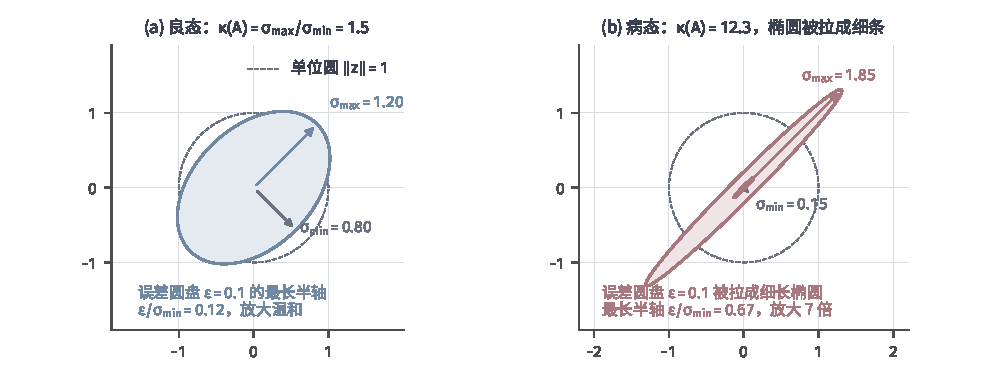
\includegraphics[width=169.0mm]{figures/00-shared/mathematical-preliminaries-upper/02-linear-spaces/matplotlib/ls-condition-number-amplification/ls-condition-number-amplification.pdf}
 \caption{条件数对误差圆盘的放大。灰虚线为单位圆$\lVert\bm z\rVert=1$；左为良态
 $\bm A_1=[[1,0.2],[0.2,1]]$，奇异值$1.20$与$0.80$，$\kappa_2=1.5$，像椭圆接近
 圆；右为病态$\bm A_2=[[1,0.85],[0.85,1]]$，奇异值$1.85$与$0.15$，$\kappa_2\approx12.3$，
 像被拉成细条。半径$\varepsilon=0.1$的误差圆盘（红）最长半轴为$\varepsilon/\sigma_{\min}$：
 良态为$0.125$，病态约$0.67$。}
 \label{fig:ls-condition-number-amplification}
\end{figure*}

当$\bm z\neq\bm0$且$F(\bm z)\neq\bm0$时，把输入、输出都换成相对尺度，得到\term{相对条件数}（relative condition number）
\[
 \kappa_{\mathrm{rel}}(F;\bm z)
 =\lim_{\delta\to0}\ \sup_{0<\lVert\Delta\bm z\rVert\leq\delta}
 \frac{\lVert\Delta\bm y\rVert/\lVert F(\bm z)\rVert}
      {\lVert\Delta\bm z\rVert/\lVert\bm z\rVert}.
\]
对线性作用，$\kappa_{\mathrm{rel}}(\bm A;\bm x)=\lVert\bm A\rVert\lVert\bm x\rVert/\lVert\bm A\bm x\rVert$随$\bm x$变化：$\bm x$落在被压缩的方向上时，输出$\bm A\bm x$小，相对条件数大；落在主伸缩方向上时它小。对可逆方阵再对所有$\bm x$取最坏，令$\bm y=\bm A\bm x$，
\[
 \sup_{\bm x\neq\bm0}\frac{\lVert\bm A\rVert\lVert\bm x\rVert}{\lVert\bm A\bm x\rVert}
 =\lVert\bm A\rVert\sup_{\bm y\neq\bm0}\frac{\lVert\bm A^{-1}\bm y\rVert}{\lVert\bm y\rVert}
 =\lVert\bm A\rVert\,\lVert\bm A^{-1}\rVert ,
\]
这个只依赖矩阵的数就是矩阵的条件数。

\begin{definition}[可逆矩阵的条件数]
\label{def:matrix-analysis-condition-number}
对同一向量范数诱导的矩阵范数，可逆方阵$\bm A$的\term{条件数}（condition number）为
\begin{equation}
 \kappa(\bm A)=\lVert\bm A\rVert\,\lVert\bm A^{-1}\rVert .
 \label{eq:matrix-analysis-condition-number}
\end{equation}
\end{definition}
由第~\ref{sec:ls-svd}节，欧氏范数下$\lVert\bm A\rVert_2=\sigma_{\max}$、$\lVert\bm A^{-1}\rVert_2=1/\sigma_{\min}$，故
\begin{equation}
 \kappa_2(\bm A)=\frac{\sigma_{\max}(\bm A)}{\sigma_{\min}(\bm A)},
 \label{eq:matrix-analysis-spectral-condition-number}
\end{equation}
即最强放大与最弱放大之比。条件数总不小于$1$，因为$1=\lVert\bm I\rVert=\lVert\bm A\bm A^{-1}\rVert\leq\lVert\bm A\rVert\lVert\bm A^{-1}\rVert=\kappa(\bm A)$。正交矩阵的奇异值全为$1$，所以$\kappa_2=1$。在$\sigma_{\max}$保持固定尺度时，$\sigma_{\min}$趋于零会使$\kappa_2$增大，与图~\ref{fig:ls-condition-number-amplification}右侧的细长椭圆一致。若所有奇异值按同一比例缩小，条件数却不变，例如$\varepsilon\bm I$的条件数始终为$1$。条件数接近$1$的问题称为良态，条件数很大的问题称为病态。

\begin{theorem}[条件数基本界]
\label{thm:matrix-analysis-condition-number-bound}
设$\kappa(F;\bm z)$为任务$F$在$\bm z$处的相对条件数，则足够小的输入扰动满足
\begin{equation}
 \frac{\lVert\Delta\bm y\rVert}{\lVert F(\bm z)\rVert}
 \lesssim\kappa(F;\bm z)\,\frac{\lVert\Delta\bm z\rVert}{\lVert\bm z\rVert}.
 \label{eq:matrix-analysis-condition-number-bound}
\end{equation}
特别地，对可逆系统$\bm A\bm x=\bm b$且$\bm b\neq\bm0$，右端扰动$\Delta\bm b$引起的解扰动对任意大小的$\Delta\bm b$都满足$\lVert\Delta\bm x\rVert/\lVert\bm x\rVert\leq\kappa(\bm A)\lVert\Delta\bm b\rVert/\lVert\bm b\rVert$。
\end{theorem}
\begin{proof}
第一式是相对条件数定义的直接改写，$\lesssim$表示忽略比$\lVert\Delta\bm z\rVert$高阶的小量。对方程，$\bm A(\bm x+\Delta\bm x)=\bm b+\Delta\bm b$减去$\bm A\bm x=\bm b$，得$\Delta\bm x=\bm A^{-1}\Delta\bm b$，故$\lVert\Delta\bm x\rVert\leq\lVert\bm A^{-1}\rVert\lVert\Delta\bm b\rVert$；又$\lVert\bm b\rVert=\lVert\bm A\bm x\rVert\leq\lVert\bm A\rVert\lVert\bm x\rVert$，即$1/\lVert\bm x\rVert\leq\lVert\bm A\rVert/\lVert\bm b\rVert$。两式相乘即得。
\end{proof}

条件数是最坏方向上的上界，不是每个扰动都达到的倍数。一般任务的相对条件数只控制足够小的扰动；矩阵本身的扰动较大时，还要考虑扰动后是否仍然可逆，这在第~\ref{chap:linear-equations-and-optimization}章估计逆矩阵与方程解的敏感度时处理。

条件数也不回答反复作用的长期结果。下面的反例中，两个矩阵的条件数相同，幂的变化趋势却相反。
\begin{example}[反例：条件数相同而幂的趋势相反]
\label{ex:ls-condition-number-vs-powers}
给定同阶的$2\bm I$与$\tfrac12\bm I$。二者的奇异值分别全为$2$与全为$\tfrac12$，所以
\[
 \begin{gathered}
\kappa_2(2\bm I)=\frac{2}{2}=1\\
\kappa_2\bigl(\tfrac12\bm I\bigr)=\frac{1/2}{1/2}=1 .
 \end{gathered}
\]
但$(2\bm I)^k=2^k\bm I$逐次增长，$(\tfrac12\bm I)^k=2^{-k}\bm I$逐次衰减。结论：条件数相同的两个矩阵，反复作用的结果可以完全相反。
\end{example}
条件数衡量一次作用的相对放大，长期行为要由谱半径判断（第~\ref{sec:ls-matrix-power-behavior}节），二者不能互相代替。

% 第6章第7节：谱的扰动（特征值的扰动、子空间之间的距离、特征子空间的转动）。

\section{矩阵的扰动}
\label{sec:ls-spectral-sensitivity}
\label{sec:linear-algebra-spectral-stability}
\label{sec:ch06-spectral-stability}

上一节让矩阵保持不变，只扰动输入向量。实际中矩阵本身也来自数据：协方差矩阵由有限样本估计，系数矩阵经过测量和舍入。这时谱分解的输入是矩阵，输出有两类：特征值（或奇异值）与特征子空间（或奇异子空间）。矩阵受到扰动$\bm E$后，它们分别移动多少？

本节先证明对称矩阵的特征值与任意矩阵的奇异值移动不超过$\lVert\bm E\rVert_2$，并说明非对称矩阵的特征值为何没有这样的保证；再建立一个与基的选取无关的子空间距离；最后证明特征子空间转过的角度由扰动与特征值间隔之比控制。

\subsection{基本矩阵运算的扰动}

同样的增量展开适用于第~\ref{chap:linear-operations}章的基本运算。先看加法。和的增量是$\Delta(\bm x+\bm y)=\Delta\bm x+\Delta\bm y$，由三角不等式，$\lVert\Delta(\bm x+\bm y)\rVert\leq\lVert\Delta\bm x\rVert+\lVert\Delta\bm y\rVert$，所以加法本身不放大绝对误差。但$\bm x\approx-\bm y$时理想输出很小，相对误差被小分母放大，下面的例子给出具体数值。
\begin{example}[加法中的抵消]
\label{ex:ls-cancellation-relative-error}
给定$x=1.0001$、$y=-1.0000$，二者各带至多$5\times10^{-5}$的绝对误差，相对误差约为$5\times10^{-5}$。理想和为$x+y=10^{-4}$，而和的绝对误差至多为$5\times10^{-5}+5\times10^{-5}=10^{-4}$，所以和的相对误差可达
\[
 \frac{10^{-4}}{10^{-4}}=1 .
\]
结论：输入的相对误差约为$5\times10^{-5}$，输出的相对误差却可达$1$，放大约$2\times10^4$倍。
\end{example}
这种抵消不是算法失误，而是问题本身在相对尺度下病态。

再看乘积。它满足
\[
 (\bm A+\bm E)(\bm B+\bm F)-\bm A\bm B=\bm A\bm F+\bm E\bm B+\bm E\bm F,
\]
前两项是一阶响应，各被另一个因子的范数放大，末项在小扰动下是二阶量。

最后看行列式。在某些接近奇异的矩阵附近，即使矩阵的相对变化很小，行列式的相对变化也可能很大。
\begin{example}[接近奇异时的行列式]
\label{ex:ls-determinant-near-singular}
给定$\bm A=\operatorname{diag}(1,\varepsilon)$，$0<\varepsilon<1$，则$\det\bm A=\varepsilon$。把第二个对角元改为$\varepsilon+\delta$，矩阵的相对变化为$\lVert\Delta\bm A\rVert_2/\lVert\bm A\rVert_2=|\delta|$，行列式变为$\varepsilon+\delta$，相对变化为
\[
 \frac{|(\varepsilon+\delta)-\varepsilon|}{\varepsilon}=\frac{|\delta|}{\varepsilon}.
\]
结论：行列式的相对误差是矩阵相对误差的$1/\varepsilon$倍，矩阵越接近奇异，放大越强。
\end{example}

这些例子说明，对不同运算需要分别检查输入、输出及误差尺度。接下来把矩阵本身作为输入，考察其特征值、奇异值和特征子空间受到扰动后的变化。

\subsection{特征值的扰动}
\label{sec:ls-spectral-value-sensitivity}

先看特征值。实对称矩阵的特征值全为实数，可以把扰动前后的特征值都按降序排列，记为$\lambda_1\geq\cdots\geq\lambda_d$与$\widetilde\lambda_1\geq\cdots\geq\widetilde\lambda_d$，再按同一次序逐个比较。对正定矩阵$\bm A$，椭圆$\{\bm x:\bm x^\top\bm A\bm x\leq1\}$的主轴沿特征方向，半轴长为$1/\sqrt\lambda$。图~\ref{fig:ls-perturbation-ellipse}画出$\bm A$换成$\bm A+\bm E$前后的两个椭圆：半轴长微变，主轴微转。

\begin{figure}[htbp]
 \centering
 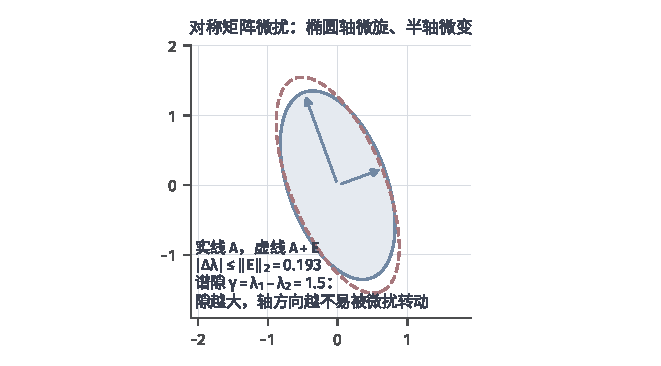
\includegraphics[width=112mm]{figures/00-shared/mathematical-preliminaries-upper/02-linear-spaces/matplotlib/ls-perturbation-ellipse/ls-perturbation-ellipse.pdf}
 \caption{对称矩阵微扰的谱与方向。实线椭圆为$\bm A$（特征值$2$与$0.5$，主轴
 方向$20^\circ$），虚线为$\bm A+\bm E$（$\lVert\bm E\rVert_2\approx0.193$）：轴
 微旋、半轴微变。新特征值约$2.18$与$0.37$，偏移$0.18$、$0.13$均小于
 $\lVert\bm E\rVert_2$，符合Weyl界；未扰动的谱隙$\delta=\lambda_1-\lambda_2=1.5$越大，
 特征方向越不易被微扰转动。}
 \label{fig:ls-perturbation-ellipse}
\end{figure}

Courant--Fischer定理把每个特征值写成Rayleigh商的最小最大值，而扰动$\bm E$对Rayleigh商的影响不超过$\lVert\bm E\rVert_2$，由此得到下面的界。
\begin{theorem}[Weyl特征值扰动界]
\label{thm:ls-weyl-eigenvalue}
对实对称$\bm A,\bm E\in\mathbb R^{d\times d}$，$\widetilde{\bm A}=\bm A+\bm E$与$\bm A$按降序配对的特征值满足
\begin{equation}
\begin{gathered}
|\widetilde\lambda_k-\lambda_k|
 \leq\lVert\bm E\rVert_2\\
k=1,\dots,d.
\end{gathered}
\label{eq:matrix-analysis-weyl-eigenvalue-perturbation}
\end{equation}
\end{theorem}
\begin{proof}
$\bm E$对称，由Rayleigh--Ritz定理，它的Rayleigh商介于最小与最大特征值之间，而它们的绝对值不超过$\lVert\bm E\rVert_2$，所以$|\bm x^\top\bm E\bm x|\leq\lVert\bm E\rVert_2\lVert\bm x\rVert_2^2$。取$\mathcal V=\operatorname{span}\{\bm q_1,\ldots,\bm q_k\}$（$\bm A$的前$k$个特征向量），其中每个$\bm x$满足
\[
 \bm x^\top\widetilde{\bm A}\bm x=\bm x^\top\bm A\bm x+\bm x^\top\bm E\bm x\geq(\lambda_k-\lVert\bm E\rVert_2)\lVert\bm x\rVert_2^2 .
\]
由Courant--Fischer定理，$\widetilde\lambda_k$不小于$\widetilde{\bm A}$在任一$k$维子空间上Rayleigh商的最小值，故$\widetilde\lambda_k\geq\lambda_k-\lVert\bm E\rVert_2$。把$\bm A$看作$\widetilde{\bm A}$加扰动$-\bm E$，交换二者的角色得$\lambda_k\geq\widetilde\lambda_k-\lVert\bm E\rVert_2$。
\end{proof}

Weyl界不需要特征值彼此分开，单重与重复特征值都适用。若$\bm A$正定且$\bm E$对称，并有$\|\bm E\|_2<\lambda_{\min}(\bm A)$，则对所有$0\leq t\leq1$，
\[
 \lambda_{\min}(\bm A+t\bm E)\geq\lambda_{\min}(\bm A)-\|\bm E\|_2>0.
\]
因此整条扰动线段都保持正定。这一统一下界将在矩阵函数微分中用于确认求逆和对数的定义域。


非对称矩阵的特征值没有这样的保证。

设$\bm A=\bm V\bm\Lambda\bm V^{-1}$可对角化，$\mu$是$\bm A+\bm E$的特征值而不是$\bm A$的特征值，$\bm w$为对应的特征向量（必要时取复数）。由$(\bm A+\bm E)\bm w=\mu\bm w$，令$\bm y=\bm V^{-1}\bm w\neq\bm0$，得$(\bm\Lambda-\mu\bm I)\bm y=-\bm V^{-1}\bm E\bm V\bm y$。$\mu$不是$\bm A$的特征值，所以对角矩阵$\bm\Lambda-\mu\bm I$可逆，于是$\bm y=-(\bm\Lambda-\mu\bm I)^{-1}\bm V^{-1}\bm E\bm V\bm y$。两边取范数并除以$\lVert\bm y\rVert_2$，得$1\leq\lVert(\bm\Lambda-\mu\bm I)^{-1}\rVert_2\,\kappa_2(\bm V)\lVert\bm E\rVert_2$；而对角矩阵$(\bm\Lambda-\mu\bm I)^{-1}$的范数是$1/\min_k|\lambda_k-\mu|$，于是得到Bauer--Fike界
\[
 \min_k|\mu-\lambda_k|\leq\kappa_2(\bm V)\lVert\bm E\rVert_2 .
\]
特征向量越接近线性相关，$\kappa_2(\bm V)$越大，界越宽。对称情形$\bm V$可取正交矩阵，$\kappa_2(\bm V)=1$，界与Weyl界同量级。

不可对角化时情况更糟，特征值的移动可以远大于扰动本身。
\begin{example}[反例：特征值的移动远大于扰动]
\label{ex:ls-jordan-eigenvalue-sensitivity}
给定$\bm N=\left[\begin{smallmatrix}0&1\\0&0\end{smallmatrix}\right]$，它的特征值全为$0$。在左下角加入扰动$\varepsilon$，得
\[
\begin{gathered}
\bm N_\varepsilon=\begin{bmatrix}0&1\\\varepsilon&0\end{bmatrix}\\
p_{\bm N_\varepsilon}(z)=z^2-\varepsilon ,
\end{gathered}
\]
扰动的大小为$\lVert\bm N_\varepsilon-\bm N\rVert_2=|\varepsilon|$。$\varepsilon>0$时特征值为$\pm\sqrt\varepsilon$，移动量为$\sqrt\varepsilon$；例如$\varepsilon=10^{-10}$时特征值移动$10^{-5}$，是扰动的$10^5$倍。$\varepsilon<0$时特征值为$\pm\mathrm i\sqrt{|\varepsilon|}$，实特征值消失。结论：特征值的移动量是$O(\sqrt{|\varepsilon|})$而非$O(|\varepsilon|)$，不能由扰动的范数乘一个常数控制。
\end{example}
可见对非对称矩阵，特征值的敏感程度取决于矩阵的结构：可对角化时，移动量至多是扰动的$\kappa_2(\bm V)$倍；不可对角化时，移动量甚至不与扰动成正比。

\subsection{奇异值的扰动}

Weyl界也给出奇异值的稳定性。把$\bm A\in\mathbb R^{m\times d}$嵌入对称分块矩阵$\left[\begin{smallmatrix}\bm0&\bm A\\\bm A^\top&\bm0\end{smallmatrix}\right]$，由$\bm A\bm v_i=\sigma_i\bm u_i$、$\bm A^\top\bm u_i=\sigma_i\bm v_i$可直接验证对每个正奇异值，向量$(\bm u_i,\pm\bm v_i)$是它的特征向量，特征值为$\pm\sigma_i$，其余特征值为零；而$\bm E$嵌入后谱范数不变。对嵌入矩阵应用Weyl界，得
\begin{equation}
 |\widetilde\sigma_i-\sigma_i|\leq\lVert\bm E\rVert_2 .
 \label{eq:matrix-analysis-singular-value-perturbation}
\end{equation}
截断SVD的误差$\sigma_{k+1}$（定理~\ref{thm:ls-best-low-rank}）因而也只移动不超过$\lVert\bm E\rVert_2$。

\subsection{子空间距离与主角}
\label{sec:ls-subspace-sensitivity}

比较特征向量时先要确定比较什么。同一子空间的基可以旋转、变号，单个基向量的变化不能当作子空间误差；特征值重复时，特征空间内部怎么换基都不改变子空间。所以比较对象必须是子空间本身，需要一个与基的选取无关的度量。图~\ref{fig:ls-principal-angles-subspaces}从两条过原点的直线看起：两直线的夹角与方向向量的选取无关；把一条直线的单位方向向量投影到另一条上，投影不掉的部分长度为$\sin\theta$。

\begin{figure}[htbp]
 \centering
 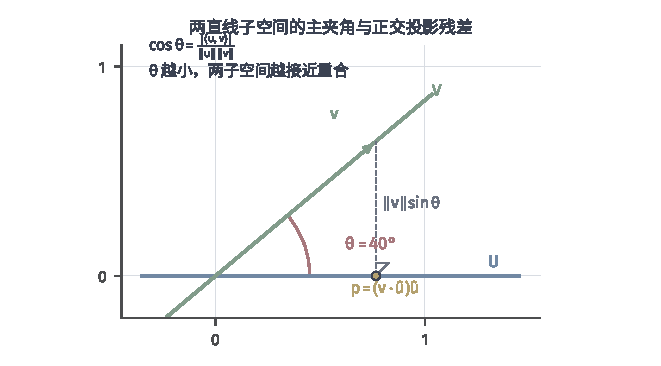
\includegraphics[width=112mm]{figures/00-shared/mathematical-preliminaries-upper/02-linear-spaces/matplotlib/ls-principal-angles-subspaces/ls-principal-angles-subspaces.pdf}
 \caption{两条直线子空间的主夹角。蓝线为$\bm U$、绿线为$\bm V$，红弧为主夹角
 $\theta=40^\circ$；黄点$\bm p$是$\bm v$在$\bm U$上的正交投影，灰虚线为投影
 垂线。$\cos40^\circ\approx0.766$、$\sin40^\circ\approx0.643$，残差长度
 $\lVert\bm v\rVert\sin\theta$即投影不掉的分量。}
 \label{fig:ls-principal-angles-subspaces}
\end{figure}

对一维子空间，若$\bm q,\widetilde{\bm q}$是单位方向向量，则$|\bm q^\top\widetilde{\bm q}|=\cos\theta$。高维子空间之间有多个夹角，由交叉内积矩阵的奇异值给出。
\begin{definition}[主夹角]
\label{def:matrix-analysis-principal-angles}
设$\bm Q,\widetilde{\bm Q}\in\mathbb R^{d\times r}$列标准正交，分别张成$r$维子空间。交叉矩阵$\bm Q^\top\widetilde{\bm Q}$的奇异值记为$\cos\theta_1\geq\dots\geq\cos\theta_r$，$0\leq\theta_1\leq\cdots\leq\theta_r\leq\pi/2$，这些$\theta_i$称为两个子空间的\term{主夹角}（principal angles）。
\end{definition}
这些奇异值都在$[0,1]$内，因为$\lVert\bm Q^\top\widetilde{\bm Q}\rVert_2\leq\lVert\bm Q\rVert_2\lVert\widetilde{\bm Q}\rVert_2=1$，所以$\theta_i$有定义。换基相当于把$\bm Q$、$\widetilde{\bm Q}$右乘正交矩阵，交叉矩阵的奇异值不变，所以主夹角只依赖子空间。

主夹角的正弦也可以直接读出。

设$\widetilde{\bm Q}_\perp$的列是$\widetilde{\bm Q}$列空间正交补的标准正交基。对单位向量$\bm a$，把$\bm Q\bm a$分解到$\widetilde{\bm Q}$的列空间与其正交补，由勾股定理，
\[
 \lVert\widetilde{\bm Q}^\top\bm Q\bm a\rVert_2^2+\lVert\widetilde{\bm Q}_\perp^\top\bm Q\bm a\rVert_2^2=\lVert\bm Q\bm a\rVert_2^2=1 .
\]
记$\bm C=\widetilde{\bm Q}^\top\bm Q$、$\bm X=\widetilde{\bm Q}_\perp^\top\bm Q$。上式对所有单位向量$\bm a$成立，说明对称矩阵$\bm X^\top\bm X$与$\bm I-\bm C^\top\bm C$的二次型处处相等，所以$\bm X^\top\bm X=\bm I-\bm C^\top\bm C$。$\bm C$是交叉矩阵的转置，奇异值为$\cos\theta_i$，所以$\bm X^\top\bm X$的特征值是$1-\cos^2\theta_i=\sin^2\theta_i$，即$\bm X$的奇异值是$\sin\theta_i$。

子空间的误差还可以用正交投影$\bm P=\bm Q\bm Q^\top$、$\widetilde{\bm P}=\widetilde{\bm Q}\widetilde{\bm Q}^\top$之差表示，它与基的选取无关。可以证明
\[
 \begin{gathered}
\lVert\bm P-\widetilde{\bm P}\rVert_2=\sin\theta_r\\
\tfrac12\lVert\bm P-\widetilde{\bm P}\rVert_{\mathrm F}^2=\sum_{i=1}^r\sin^2\theta_i .
 \end{gathered}
\]
第二式可以直接验证：由$\operatorname{tr}\bm P=\operatorname{tr}\widetilde{\bm P}=r$与$\operatorname{tr}(\bm P\widetilde{\bm P})=\lVert\bm Q^\top\widetilde{\bm Q}\rVert_{\mathrm F}^2=\sum_i\cos^2\theta_i$，得$\lVert\bm P-\widetilde{\bm P}\rVert_{\mathrm F}^2=2r-2\sum_i\cos^2\theta_i=2\sum_i\sin^2\theta_i$。第一式说明投影矩阵之差的谱范数就是最大主夹角的正弦，它的证明较长，这里从略。

\subsection{特征子空间的扰动}

有了主夹角，就可以估计扰动使特征子空间转过多大的角度。

设$\bm A$、$\widetilde{\bm A}=\bm A+\bm E$实对称，$\bm Q$的列是$\bm A$的前$k$个单位特征向量，$\widetilde{\bm Q}$的列是$\widetilde{\bm A}$的前$k$个单位特征向量。要求目标特征值与扰动后其余特征值之间有间隔
\[
 \gamma=\lambda_k-\widetilde\lambda_{k+1}>0 .
\]
记$\widetilde{\bm Q}_\perp$为$\widetilde{\bm A}$其余特征向量组成的矩阵，$\widetilde{\bm\Lambda}_2$为对应的特征值对角矩阵，$\bm\Lambda_1=\operatorname{diag}(\lambda_1,\ldots,\lambda_k)$，并令$\bm X=\widetilde{\bm Q}_\perp^\top\bm Q$。由上一小节，它的奇异值就是两个子空间主夹角的正弦。

把$\widetilde{\bm Q}_\perp^\top\widetilde{\bm A}=\widetilde{\bm\Lambda}_2\widetilde{\bm Q}_\perp^\top$右乘$\bm Q$，把$\bm A\bm Q=\bm Q\bm\Lambda_1$左乘$\widetilde{\bm Q}_\perp^\top$，两式相减，由$\widetilde{\bm A}-\bm A=\bm E$得
\[
 \widetilde{\bm\Lambda}_2\bm X-\bm X\bm\Lambda_1=\widetilde{\bm Q}_\perp^\top\bm E\bm Q .
\]
这是关于$\bm X$的线性方程，两侧的系数矩阵都是对角的，因此可以逐元素求解（第~\ref{chap:linear-equations-and-optimization}章把形如$\bm A\bm X+\bm X\bm B=\bm C$的方程称为Sylvester方程）。逐元素写出为$(\widetilde\lambda_j-\lambda_i)X_{j,i}=(\widetilde{\bm Q}_\perp^\top\bm E\bm Q)_{j,i}$，其中$i\leq k<j$。由降序，$\lambda_i-\widetilde\lambda_j\geq\lambda_k-\widetilde\lambda_{k+1}=\gamma$，逐元素相除得
\[
 \lVert\bm X\rVert_{\mathrm F}\leq\frac{\lVert\widetilde{\bm Q}_\perp^\top\bm E\bm Q\rVert_{\mathrm F}}{\gamma}\leq\frac{\lVert\bm E\bm Q\rVert_{\mathrm F}}{\gamma}.
\]
左端的平方是主夹角正弦的平方和，所以这个平方和由扰动与谱隙之比控制。更细的论证给出谱范数下的同型结论，称为Davis--Kahan谱隙界\scite{math-golub2013matrix}：
\begin{equation}
 \lVert\widetilde{\bm P}-\bm P\rVert_2=\sin\theta_{k}
 \leq\frac{\lVert\bm E\rVert_2}{\gamma}.
 \label{eq:matrix-analysis-eigenvector-gap-bound}
\end{equation}
$\gamma$用到扰动后的特征值。若只知道未扰动的谱隙$\delta=\lambda_k-\lambda_{k+1}$，由Weyl界$\widetilde\lambda_{k+1}\leq\lambda_{k+1}+\lVert\bm E\rVert_2$，得$\gamma\geq\delta-\lVert\bm E\rVert_2$；当$\lVert\bm E\rVert_2\leq\delta/2$时，$\gamma\geq\delta/2$，右端不超过$2\lVert\bm E\rVert_2/\delta$。

谱隙在分母上：谱隙越小，子空间越容易被扰动转动。下面的二维例子可以精确算出转角。
\begin{example}[谱隙与特征方向的转角]
\label{ex:ls-gap-direction-rotation}
给定$\bm A_\alpha=\operatorname{diag}(\alpha,-\alpha)$（$\alpha>0$）与交叉扰动$\bm E=\varepsilon\left[\begin{smallmatrix}0&1\\1&0\end{smallmatrix}\right]$（$\varepsilon>0$）。$\bm A_\alpha$的两个特征值相距$2\alpha$，最大特征方向是$\bm e_1$。记$r=\sqrt{\alpha^2+\varepsilon^2}$，取$\theta\in(0,\pi/4)$满足$\cos2\theta=\alpha/r$、$\sin2\theta=\varepsilon/r$，即$\theta=\tfrac12\arctan(\varepsilon/\alpha)$。扰动后的矩阵可以写成
\[
 \bm A_\alpha+\bm E=\begin{bmatrix}\alpha&\varepsilon\\\varepsilon&-\alpha\end{bmatrix}
 =r\begin{bmatrix}\cos2\theta&\sin2\theta\\\sin2\theta&-\cos2\theta\end{bmatrix}.
\]
由两角差公式，
\[
 (\bm A_\alpha+\bm E)\begin{bmatrix}\cos\theta\\\sin\theta\end{bmatrix}
 =r\begin{bmatrix}\cos(2\theta-\theta)\\\sin(2\theta-\theta)\end{bmatrix}
 =r\begin{bmatrix}\cos\theta\\\sin\theta\end{bmatrix},
\]
而迹为零，另一个特征值是$-r$。所以最大特征方向从$\bm e_1$转到$(\cos\theta,\sin\theta)^\top$，转角为
\[
 \theta=\tfrac12\arctan\frac{\varepsilon}{\alpha}\approx\frac{\varepsilon}{2\alpha}\qquad(\varepsilon\ll\alpha).
\]
与界~\eqref{eq:matrix-analysis-eigenvector-gap-bound}比较：$\lVert\bm E\rVert_2=\varepsilon$，$\gamma=\lambda_1-\widetilde\lambda_2=\alpha+r\approx2\alpha$，界给出$\sin\theta\leq\varepsilon/\gamma\approx\varepsilon/(2\alpha)$，与实际转角同阶。结论：转角近似与谱隙$2\alpha$成反比，$\alpha$减半，转角加倍。
\end{example}
图~\ref{fig:matrix-analysis-gap-direction}画出这一关系。

谱隙只需存在于目标特征值组与组外之间，组内的特征值不必彼此分开。例如在$\operatorname{diag}(2,2,0)$中，特征值$2$对应的平面内每个单位向量都是特征方向，单独比较某个向量没有意义。但取$k=2$，未扰动的谱隙为$\delta=2-0=2$，由上面的推论，$\lVert\bm E\rVert_2\leq1$时整个二维特征子空间的最大主夹角满足$\sin\theta_2\leq2\lVert\bm E\rVert_2/\delta=\lVert\bm E\rVert_2$。

奇异子空间也有同样的结论。对第~\ref{sec:ls-spectral-value-sensitivity}节的对称嵌入矩阵$\left[\begin{smallmatrix}\bm0&\bm A\\\bm A^\top&\bm0\end{smallmatrix}\right]$作同样的谱隙论证，可知奇异子空间的稳定性由截断处的间隔$\sigma_k-\sigma_{k+1}$控制。所以截断SVD的误差$\sigma_{k+1}$总是稳定的，它所用的主方向却只在截断处有间隔时才稳定。

\begin{figure}
 \centering
 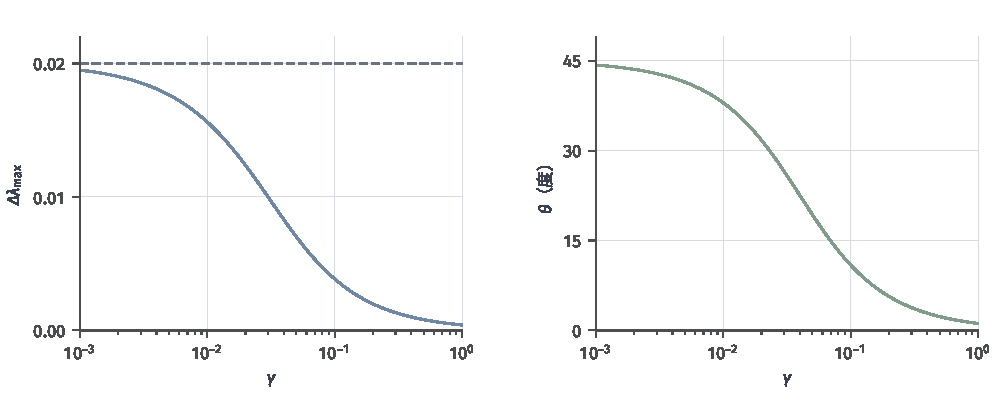
\includegraphics[width=0.92\linewidth]{figures/00-shared/mathematical-preliminaries-upper/02-linear-spaces/matplotlib/matrix-analysis-gap-direction/figure.pdf}
 \caption{谱隙方向示意：$\bm A_\alpha$的两个特征值相距$2\alpha$（谱隙），
 交叉扰动$\varepsilon$把最大特征方向转过约$\varepsilon/(2\alpha)$；
 谱隙越小，同样扰动转过的角度越大。}
 \label{fig:matrix-analysis-gap-direction}
\end{figure}

本节得到的结论是：把矩阵本身当作输入时，对称矩阵的特征值与任意矩阵的奇异值都是良态的，移动不超过$\lVert\bm E\rVert_2$，不要求特征值彼此分开；特征子空间要用与基无关的主夹角比较，它的转角由扰动与谱隙之比控制，谱隙越小越容易被转动；非对称矩阵的特征值可能对扰动非常敏感，敏感程度由特征向量矩阵的条件数或不可对角化的结构决定。条件数与谱的扰动讨论的都是一次作用或一次分解。下一节转向同一个矩阵的反复作用。

% 第6章第8节：矩阵的长期作用（谱半径判据、衰减速度与边界情形、瞬态放大、Neumann级数）。

\section{矩阵的长期作用}
\label{sec:ls-convergence}
\label{sec:linear-algebra-convergence-approximation}
\label{sec:ls-matrix-power-behavior}
\label{sec:linear-algebra-power-convergence}

最大奇异值衡量一次作用对绝对误差的最大放大，条件数则刻画相对误差的放大。迭代法、离散动态系统和许多学习算法却反复施加同一个线性作用，得到序列$\bm x^{(k)}=\bm A^k\bm x^{(0)}$；把这些作用累加起来，又得到矩阵级数。本节回答两个问题。第一，矩阵幂什么时候对所有初值都趋于零，趋近得多快，途中会不会先变大？第二，由矩阵幂组成的级数什么时候收敛，收敛到什么？

讨论收敛时不必担心范数的选择。第~\ref{sec:ls-finite-dimensional-sequences}节已经说明，有限维空间上的任意两个范数彼此等价（定理~\ref{thm:ls-norm-equivalence}），向量或矩阵序列是否收敛与所用范数无关，换范数只改变不等式中的常数。所以下面可以在任意方便的范数下论证，结论对所有范数成立。我们将看到，长期行为由谱半径决定，早期的放大则取决于矩阵是否正规。

\subsection{矩阵幂的收敛判据}

对固定方阵$\bm A$反复作用，初值$\bm x^{(0)}$在第$k$步变成$\bm x^{(k)}=\bm A^k\bm x^{(0)}$。只检查一个初值的轨迹不够：若初值恰好不含某个增长方向的分量，轨迹看起来收敛，换一个初值就发散。下面的反例说明这一点。
\begin{example}[反例：收敛与发散的轨迹]
\label{ex:ls-partial-convergence}
给定$\bm A=\operatorname{diag}(0.5,2)$，比较两个初值的轨迹：
\[
\begin{gathered}
\bm A^k\begin{bmatrix}1\\0\end{bmatrix}=\begin{bmatrix}0.5^k\\0\end{bmatrix}\to\bm0\\
\bm A^k\begin{bmatrix}0\\1\end{bmatrix}=\begin{bmatrix}0\\2^k\end{bmatrix},
\end{gathered}
\]
其中后一条轨迹的长度为$2^k\to\infty$。
结论：初值$(1,0)^\top$不含增长方向$\bm e_2$的分量，轨迹收敛；初值$(0,1)^\top$的轨迹发散。一个初值的轨迹收敛，不能说明矩阵幂趋于零。
\end{example}
所以要问的是：何时对全体初值都有$\bm A^k\bm x^{(0)}\to\bm0$？逐个取$\bm x^{(0)}=\bm e_j$可知，这等价于$\bm A^k$的每一列趋于零，即$\bm A^k\to\bm0$。

图~\ref{fig:ls-spectral-radius-convergence}显示了最简单的正规情形：误差每步乘以$\rho$，$\rho<1$时衰减，$\rho>1$时增长。

\begin{figure*}[htbp]
 \centering
 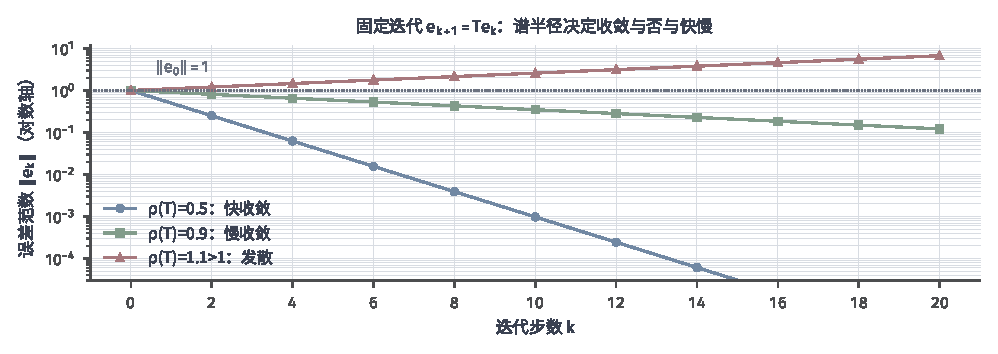
\includegraphics[width=169.0mm]{figures/00-shared/mathematical-preliminaries-upper/02-linear-spaces/matplotlib/ls-spectral-radius-convergence/ls-spectral-radius-convergence.pdf}
 \caption{谱半径决定迭代的长期方向。递推$\bm e^{(t+1)}=\bm A\bm e^{(t)}$、
 $\lVert\bm e^{(0)}\rVert=1$，取正规矩阵$\bm A=\rho\bm I$时$\lVert\bm e^{(t)}\rVert=\rho^t$：
 $\rho=0.5$（蓝）约十四步降到$10^{-4}$，$\rho=0.9$（绿）缓慢下降，
 $\rho=1.1$（红）指数上升。纵轴为半对数。}
 \label{fig:ls-spectral-radius-convergence}
\end{figure*}

最先想到的判据来自范数。由次乘性，$\lVert\bm A^k\rVert\leq\lVert\bm A\rVert^k$，所以只要在某个次乘性矩阵范数下$\lVert\bm A\rVert<1$，就有$\bm A^k\to\bm0$。但这只是充分条件：示例~\ref{ex:ls-nonnormal-norm-radius}的矩阵$\left[\begin{smallmatrix}0.8&4\\0&0.5\end{smallmatrix}\right]$二范数大于$4$，而示例~\ref{ex:ls-triangular-power}已经算出它的幂按$0.8^k$与$0.5^k$趋于零，它的谱半径也只有$0.8$。正规矩阵的范数等于谱半径；非正规矩阵的Schur形可能含有非对角块，或含有不呈模长乘旋转形式的$2\times2$对角块。这些结构可能使范数大于谱半径，但不保证二者一定不同。下面的引理先用相似变换把每个对角块化为模长乘旋转，再用一次坐标缩放把非对角块压小，从而把谱半径变成一个可用的几何上界。

\begin{lemma}[矩阵幂的几何上界]
\label{lem:ls-power-geometric-bound}
对任意$r>\rho(\bm A)$，存在常数$C_r$，使$\lVert\bm A^k\rVert_2\leq C_rr^k$对所有$k\geq0$成立；等价地，存在一个向量范数，使$\bm A$在它诱导的矩阵范数下不超过$r$。
\end{lemma}
\begin{proof}
取实Schur形$\bm A=\bm Q\bm T\bm Q^\top$，设$\bm T$有$s$个对角块，第$i$块的特征值模长为$|\lambda_i|$。

先处理对角块。每个$2\times2$对角块$\bm T_{i,i}$有一对共轭特征值，按第~\ref{sec:ls-general-square-spectrum}节的论证，在复特征向量的实部、虚部组成的基下，它化为模长乘旋转：$\bm T_{i,i}=\bm P_i(|\lambda_i|\bm R_i)\bm P_i^{-1}$，$\bm R_i$为旋转矩阵；$1\times1$块取$\bm P_i=1$、$\bm R_i=\pm1$。

再压小非对角块。对$0<\varepsilon\leq1$，令分块对角矩阵
\[
 \bm D_\varepsilon=\operatorname{diag}(\varepsilon^{0}\bm P_1,\varepsilon^{1}\bm P_2,\ldots,\varepsilon^{s-1}\bm P_s).
\]
直接相乘，$\bm D_\varepsilon^{-1}\bm T\bm D_\varepsilon$的第$(i,j)$块为$\varepsilon^{j-i}\bm P_i^{-1}\bm T_{i,j}\bm P_j$：对角块是$|\lambda_i|\bm R_i$，二范数不超过$\rho(\bm A)$；$j>i$的块带有因子$\varepsilon^{j-i}\leq\varepsilon$，所以全部非对角块的Frobenius范数不超过$\varepsilon c$，其中$c$与$\varepsilon$无关。把矩阵拆成分块对角部分与非对角部分，得
\[
 \lVert\bm D_\varepsilon^{-1}\bm T\bm D_\varepsilon\rVert_2\leq\rho(\bm A)+\varepsilon c .
\]
取$\varepsilon$足够小，使右端不超过$r$。

最后换回原坐标。令$\bm M=\bm Q\bm D_\varepsilon$，则$\bm A=\bm M(\bm D_\varepsilon^{-1}\bm T\bm D_\varepsilon)\bm M^{-1}$，中间各对$\bm M^{-1}\bm M$相消，$\bm A^k=\bm M(\bm D_\varepsilon^{-1}\bm T\bm D_\varepsilon)^k\bm M^{-1}$，故
\[
 \lVert\bm A^k\rVert_2\leq\lVert\bm M\rVert_2\lVert\bm M^{-1}\rVert_2\,r^k ,
\]
取$C_r=\lVert\bm M\rVert_2\lVert\bm M^{-1}\rVert_2$即可。所求的向量范数取$\bm x\mapsto\lVert\bm M^{-1}\bm x\rVert_2$，它诱导的$\bm A$的范数等于$\lVert\bm M^{-1}\bm A\bm M\rVert_2=\lVert\bm D_\varepsilon^{-1}\bm T\bm D_\varepsilon\rVert_2\leq r$。
\end{proof}

有了这个上界，就能给出矩阵幂衰减的充要条件。
\begin{theorem}[矩阵幂的衰减判据]
\label{thm:ls-power-decay}
对实方阵$\bm A$，$\bm A^k\to\bm0$当且仅当$\rho(\bm A)<1$。
\end{theorem}
\begin{proof}
充分性：取$r$满足$\rho(\bm A)<r<1$，由引理，$\lVert\bm A^k\rVert_2\leq C_rr^k\to0$。必要性：设有特征值$|\lambda|\geq1$。若$\lambda$为实数，其特征向量$\bm v$满足$\lVert\bm A^k\bm v\rVert=|\lambda|^k\lVert\bm v\rVert\not\to0$；若$\lambda$非实，在对应的二维不变子空间中，$\bm A^k$在基$(\bm u,\bm w)$下的矩阵是$|\lambda|^k$乘一个旋转，$\bm A^k\bm u$的坐标长度为$|\lambda|^k\geq1$，不趋于零。两种情形都有$\bm A^k\not\to\bm0$。
\end{proof}

\subsection{收敛速率与临界情形}

判据只回答矩阵幂是否趋于零，同一论证还给出衰减速度。上界$\lVert\bm A^k\rVert\leq C_rr^k$对任意$r>\rho(\bm A)$成立；必要性证明中的特征方向（或不变平面）给出下界$\lVert\bm A^k\rVert\geq c\,\rho(\bm A)^k$，$c>0$为常数。两边开$k$次方，$C_r^{1/k}$与$c^{1/k}$都趋于$1$，于是$\rho(\bm A)\leq\liminf_k\lVert\bm A^k\rVert^{1/k}\leq\limsup_k\lVert\bm A^k\rVert^{1/k}\leq r$。令$r$趋于$\rho(\bm A)$，得到Gelfand公式
\begin{equation}
 \rho(\bm A)=\lim_{k\to\infty}\lVert\bm A^k\rVert^{1/k}.
 \label{eq:ls-gelfand-formula}
\end{equation}
由范数等价（定理~\ref{thm:ls-norm-equivalence}），换成任意矩阵范数只改变常数，开$k$次方后常数的影响消失，所以公式对任意矩阵范数成立。由$\lVert\bm A^k\rVert\leq\lVert\bm A\rVert^k$还得$\rho(\bm A)\leq\lVert\bm A\rVert$对任意次乘性范数成立。

Gelfand公式说明，谱半径是矩阵幂的最大放大倍数的长期几何平均。它不表示每个初值的误差都逐步乘以$\rho(\bm A)$：某些初值可能不含最慢衰减方向，非正规作用还可能在早期放大误差。

若粗略用$\rho^m$估计长期倍率，且$0<\rho<1$，由$\rho^m=1/10$得到参考步数$m=1/\log_{10}(1/\rho)$。例如$\rho=0.5$时约为$3.3$，$\rho=0.99$时约为$229$；实际达到目标的步数还取决于初值和有限步的放大。

$\rho(\bm A)=1$是边界情形，结果还取决于模为$1$的特征值及其对应结构。特征值$1$的特征方向保持不动，$-1$的特征方向来回翻转，模为$1$的非实特征值对应纯旋转；在这些方向上$\bm A^k$不趋于零，但保持有界。若模为$1$的特征值缺少足够的特征向量，还会出现增长。
\begin{example}[反例：谱半径为$1$而矩阵幂无界]
\label{ex:ls-unit-spectral-radius-growth}
给定$\bm J_1=\left[\begin{smallmatrix}1&1\\0&1\end{smallmatrix}\right]$，它只有特征值$1$，$\rho(\bm J_1)=1$，特征向量只有$(1,0)^\top$的倍数。按示例~\ref{ex:ls-jordan-block-power}的二项式展开，把$0.8$换成$1$，得
\[
 \bm J_1^k=(\bm I+\bm N)^k=\bm I+k\bm N=\begin{bmatrix}1&k\\0&1\end{bmatrix}.
\]
结论：右上角随$k$线性增长，$\lVert\bm J_1^k\rVert_2\geq k\to\infty$；谱半径等于$1$不能保证矩阵幂有界。
\end{example}
$\rho(\bm A)>1$时，由定理~\ref{thm:ls-power-decay}必要性的证明，从模大于$1$的特征值的特征方向（或不变平面）出发的轨迹不趋于零；但如示例~\ref{ex:ls-partial-convergence}所示，不必每个初值都发散。

\subsection{非正规矩阵的瞬态增长}

$\rho(\bm A)<1$保证最终衰减，但不说明途中的情况。下面的例子中，轨迹先变长、后衰减。
\begin{example}[非正规矩阵的瞬态放大]
\label{ex:ls-transient-growth}
给定迭代
\begin{equation}
\begin{gathered}
\bm A=\begin{bmatrix}0.8&4\\0&0.5\end{bmatrix}\\
\bm x^{(k+1)}=\bm A\bm x^{(k)}\\
\bm x^{(0)}=(0,1)^{\top}.
\end{gathered}
\label{eq:ch06-fixed-iteration-example}
\end{equation}
示例~\ref{ex:ls-triangular-power}已把初值沿特征向量$\bm v_1=(1,0)^{\top}$、$\bm v_2=(-40/3,1)^{\top}$分解为$\bm x^{(0)}=\tfrac{40}{3}\bm v_1+\bm v_2$，并写出了矩阵幂与轨迹：
\begin{equation}
\begin{gathered}
\bm A^k=
 \begin{bmatrix}
  0.8^k&\frac{40}{3}(0.8^k-0.5^k)\\
  0&0.5^k
 \end{bmatrix}\\
\bm x^{(k)}=
 \begin{bmatrix}\frac{40}{3}(0.8^k-0.5^k)\\0.5^k\end{bmatrix}.
\end{gathered}
\label{eq:ch06-diagonalizable-finite-trajectory}
\end{equation}
代入$k=1,2,3$得
\[
\begin{gathered}
\bm x^{(1)}=\begin{bmatrix}4\\0.5\end{bmatrix}\\
\bm x^{(2)}=\begin{bmatrix}5.2\\0.25\end{bmatrix}\\
\bm x^{(3)}=\begin{bmatrix}5.16\\0.125\end{bmatrix},
\end{gathered}
\]
长度分别约为$4.03$、$5.21$、$5.16$，都远大于初值的长度$1$。另一方面$\rho(\bm A)=0.8<1$，由定理~\ref{thm:ls-power-decay}，轨迹最终趋于零。结论：谱半径小于$1$时，轨迹仍可以先放大数倍、再衰减。
\end{example}
放大的原因在于初值的分解。$\tfrac{40}{3}\bm v_1=(40/3,0)^\top$与$\bm v_2=(-40/3,1)^\top$都很长、方向几乎相反，初值$(0,1)^\top$由二者相消而成。两个分量衰减速度不同，相消很快被打破，所以长度先增后降（图~\ref{fig:ch06-transient-growth}）。

\begin{figure*}[htbp]
  \centering
  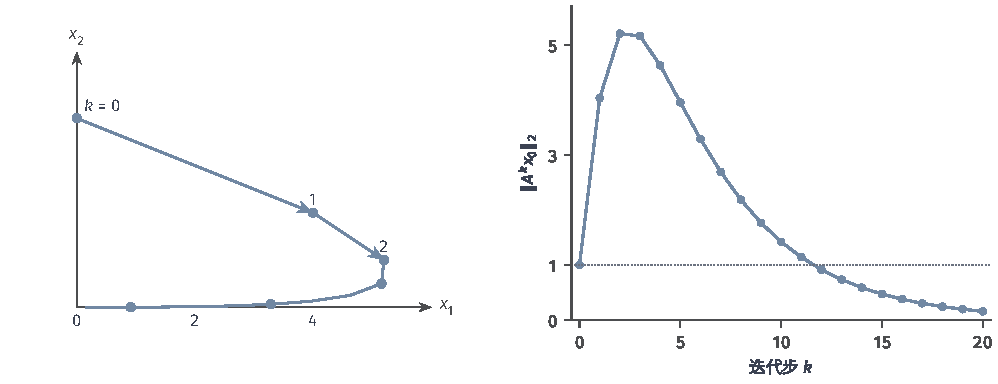
\includegraphics[width=169.0mm]{figures/00-shared/mathematical-preliminaries-upper/02-linear-spaces/matplotlib/ch06-transient-growth/figure.pdf}
  \caption{固定二维矩阵的反复作用。初值为$(0,1)^{\top}$，前两步的长度增加，
  此后回到原点；右图将长度与初始长度$1$比较。特征值$0.8$和$0.5$决定长期衰减，
  非正交特征方向间的相消则决定早期放大。两图使用同一个矩阵和同一组迭代点。}
  \label{fig:ch06-transient-growth}
\end{figure*}

一般地，可对角化矩阵$\bm A=\bm V\bm\Lambda\bm V^{-1}$满足$\bm A^k=\bm V\bm\Lambda^k\bm V^{-1}$，所以
\[
 \lVert\bm A^k\rVert_2\leq\lVert\bm V\rVert_2\lVert\bm V^{-1}\rVert_2\,\rho(\bm A)^k .
\]
特征向量越接近线性相关，$\lVert\bm V\rVert_2\lVert\bm V^{-1}\rVert_2$越大，早期可能的放大越强。正规矩阵则满足$\lVert\bm A^k\rVert_2=\rho(\bm A)^k$（第~\ref{sec:ls-general-square-spectrum}节），不会出现瞬态放大。

不可对角化时，特征向量本身就不够，矩阵幂中还会出现多项式因子。考虑$s$阶矩阵$\bm J=\lambda\bm I+\bm N$，其中$\bm N$是超对角元为$1$、其余元素为零的矩阵，满足$\bm N^s=\bm0$；这样的矩阵称为Jordan块，示例~\ref{ex:ls-jordan-block-power}的$\bm J$是$s=2$的情形。$\lambda\bm I$与$\bm N$可交换，二项式展开成立，且$j\geq s$的项为零：
\begin{equation}
 \bm J^k=\sum_{j=0}^{\min(k,s-1)}\binom{k}{j}\lambda^{k-j}\bm N^j .
 \label{eq:ch06-jordan-power}
\end{equation}
$\binom kj$是$k$的至多$s-1$次多项式，而多项式增长慢于几何衰减，$k^{s-1}|\lambda|^k\to0$（$|\lambda|<1$）。所以$|\lambda|<1$时块幂仍趋于零，只是起初可能上升。下面用二阶块看这种先升后降。
\begin{example}[Jordan块幂的先升后降]
\label{ex:ls-jordan-transient}
给定$\bm J=\left[\begin{smallmatrix}0.8&1\\0&0.8\end{smallmatrix}\right]$与初值$(0,1)^{\top}$。由示例~\ref{ex:ls-jordan-block-power}，
\[
 \bm J^k\begin{bmatrix}0\\1\end{bmatrix}=\begin{bmatrix}k\,0.8^{k-1}\\0.8^k\end{bmatrix}.
\]
第一坐标在$k=1,2,\ldots,6$时依次为$1$、$1.6$、$1.92$、$2.048$、$2.048$、$1.966$（末项保留三位小数），在$k=4,5$时达到最大值约$2.05$，此后才衰减。结论：特征值$0.8<1$保证最终衰减，但多项式因子$k$使第一坐标先上升到初值长度的两倍以上。
\end{example}
图~\ref{fig:vol1-add-linear-jordan-accumulation}画出这条轨迹的两个坐标。多项式因子也是引理~\ref{lem:ls-power-geometric-bound}中常数$C_r$的来源：$r$越接近$\rho(\bm A)$，需要的$\varepsilon$越小，$C_r$可能越大。

\begin{figure}[!htb]
  \centering
  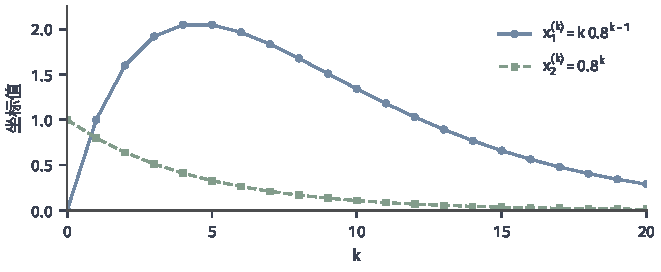
\includegraphics[width=112mm]{figures/00-shared/mathematical-preliminaries-upper/02-linear-spaces/matplotlib/comprehension-additions/linear-jordan-accumulation.pdf}
  \caption{Jordan块的累积项。取正文$\bm J=\left[\begin{smallmatrix}0.8&1\\0&0.8\end{smallmatrix}\right]$与初值$(0,1)^{\top}$。绿线为$0.8^k$，蓝线在$k\geq1$时为$k0.8^{k-1}$，在$k=0$时为$0$。点表示整数步，连线仅引导读图；两坐标最终都趋零。}
  \label{fig:vol1-add-linear-jordan-accumulation}
\end{figure}

所以报告迭代的收敛性时，要分开两件事：谱半径给出长期速度，特征向量的病态程度或Jordan块决定早期可能的放大。

\subsection{Neumann级数与累积误差}
\label{sec:ls-matrix-series-exponential}

把矩阵幂累加起来会得到什么？最常用的是$\sum_k\bm A^k$，它把求逆$(\bm I-\bm A)^{-1}$写成反复作用之和，也描述每步注入的误差怎样累积。这里说矩阵级数$\sum_{k=0}^{\infty}\bm A^k$收敛，指部分和$\bm S_N=\sum_{k=0}^N\bm A^k$作为矩阵序列收敛。对标量$a$，$|a|<1$时几何级数$\sum_ka^k=1/(1-a)$；矩阵情形有同样的结论。

\begin{theorem}[Neumann级数与逆]
\label{thm:ls-neumann}
若在某个次乘性矩阵范数下$\lVert\bm A\rVert<1$，则级数$\sum_{k=0}^{\infty}\bm A^k$收敛，$\bm I-\bm A$可逆，且
\begin{equation}
 (\bm I-\bm A)^{-1}=\sum_{k=0}^{\infty}\bm A^k,
 \label{eq:ls-neumann-series}
\end{equation}
截断尾项满足$\lVert\sum_{k>N}\bm A^k\rVert\leq\lVert\bm A\rVert^{N+1}/(1-\lVert\bm A\rVert)$。
\end{theorem}
\begin{proof}
由次乘性，$\sum_k\lVert\bm A^k\rVert\leq\sum_k\lVert\bm A\rVert^k<\infty$。由范数等价（定理~\ref{thm:ls-norm-equivalence}），每个元素的绝对值不超过常数乘$\lVert\bm A^k\rVert$，所以每个元素的级数绝对收敛，矩阵级数收敛到某个$\bm S$；尾界由几何级数求和得到。逐项相消，$(\bm I-\bm A)\bm S_N=\bm S_N(\bm I-\bm A)=\bm I-\bm A^{N+1}$，令$N\to\infty$，$\bm A^{N+1}\to\bm0$，得$(\bm I-\bm A)\bm S=\bm S(\bm I-\bm A)=\bm I$。
\end{proof}
条件$\lVert\bm A\rVert<1$可以放宽到谱半径。由引理~\ref{lem:ls-power-geometric-bound}，只要$\rho(\bm A)<1$，就存在使$\lVert\bm A\rVert<1$的诱导范数，所以级数在$\rho(\bm A)<1$时收敛，只是尾界要在那个范数中读取；反之$\rho(\bm A)\geq1$时，由定理~\ref{thm:ls-power-decay}，通项$\bm A^k$不趋于零，级数发散。图~\ref{fig:ls-neumann-series-tail}用一个$2\times2$例子核对尾界。

\begin{figure}[htbp]
 \centering
 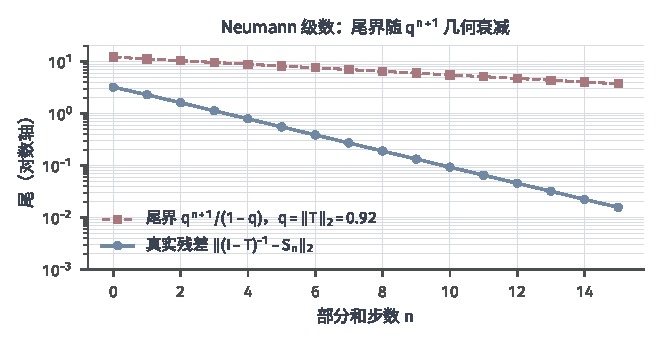
\includegraphics[width=112mm]{figures/00-shared/mathematical-preliminaries-upper/02-linear-spaces/matplotlib/ls-neumann-series-tail/ls-neumann-series-tail.pdf}
 \caption{Neumann级数尾界。$\bm T=[[0.7,0.6],[0,0.1]]$，$q=\lVert\bm T\rVert_2
 \approx0.924<1$，$(\bm I-\bm T)^{-1}=\sum\bm T^k$。蓝线为真实残差
 $\lVert\bm R_n\rVert=\lVert\bm T^{n+1}(\bm I-\bm T)^{-1}\rVert$，红虚线为尾界
 $q^{n+1}/(1-q)$，纵轴半对数（$n=0,\dots,15$）。}
 \label{fig:ls-neumann-series-tail}
\end{figure}

\paragraph{持续扰动的累积}

同样的级数描述持续扰动的累积。迭代的每一步都可能引入新误差（例如舍入），递推成为$\bm e^{(t+1)}=\bm T\bm e^{(t)}+\bm\delta^{(t)}$，$\bm\delta^{(t)}$是第$t$步注入的误差。逐步展开，
\[
 \bm e^{(t)}=\bm T^t\bm e^{(0)}+\sum_{j=0}^{t-1}\bm T^{t-1-j}\bm\delta^{(j)} .
\]
若在某个范数下$\lVert\bm T\rVert\leq q<1$且$\lVert\bm\delta^{(j)}\rVert\leq\delta$，第二项不超过$\delta\sum_{i\geq0}q^i$，于是
\begin{equation}
 \lVert\bm e^{(t)}\rVert\leq q^t\lVert\bm e^{(0)}\rVert+\frac{\delta}{1-q}.
 \label{eq:ls-noise-floor}
\end{equation}
初始误差几何衰减，持续扰动带来的误差由$\delta/(1-q)$这一不随$t$下降的上界控制；$q$越接近$1$，这个上界越大。它不是误差的必然下限，具体误差还取决于各步扰动。

本节的两个问题至此都有了回答。矩阵幂对全体初值衰减，当且仅当谱半径小于$1$；谱半径还是每步放大倍数的长期几何平均，决定收敛快慢。非正规矩阵在衰减之前可能先放大，放大程度由特征向量的病态程度或不可对角化的结构决定。Neumann级数在谱半径小于$1$时收敛到$(\bm I-\bm A)^{-1}$，持续注入的有界扰动则给出一个不随步数下降的误差上界。

% 第6章第9节：本章小结。

\section{本章小结}
\label{sec:ls-analysis-summary}
\label{sec:linear-algebra-summary}
\label{sec:matrix-analysis-summary}

本章围绕一个问题展开：同一个线性作用在什么样的基下最简单，从这个最简形式又能读出它的哪些性质？

前五节逐步调整对基的要求，回答前一半。由特征向量组成的基使矩阵成为对角形；特征值是特征多项式$p_{\bm A}(z)=\det(z\bm I-\bm A)$的根，不随基改变，Cayley--Hamilton定理说明$p_{\bm A}(\bm A)=\bm0$。$n$阶矩阵可对角化，当且仅当它有$n$个线性无关的实特征向量，这时$\bm A^k=\bm V\bm\Lambda^k\bm V^{-1}$。要求基标准正交时，能对角化的恰好是对称矩阵，特征值因而是Rayleigh商的极值；一般方阵只能化为实Schur形，正规矩阵化为分块对角形。输入、输出各取一组标准正交基时，任何矩阵都有奇异值分解，它给出谱范数、Frobenius范数和最佳低秩逼近。

后三节用这些最简形式读出三类性质，它们相互关联而不能互相代替。一次作用对绝对误差的最大放大由最大奇异值衡量，相对误差的放大由条件数$\kappa_2=\sigma_{\max}/\sigma_{\min}$刻画；把矩阵本身当作输入时，对称矩阵的特征值与任意矩阵的奇异值移动不超过$\lVert\bm E\rVert_2$，特征子空间的转角由扰动与谱隙之比控制，非正规矩阵的特征值则可能很敏感；反复作用的长期速度由谱半径决定，$\bm A^k\to\bm0$当且仅当$\rho(\bm A)<1$，但非正规矩阵可能先放大再衰减。第~\ref{chap:linear-equations-and-optimization}章求解线性方程、最小二乘与矩阵方程时，将用到奇异值分解、条件数、谱、Cayley--Hamilton定理与实Schur形。


\chapter{线性方程与矩阵方程}
\label{chap:linear-equations-and-optimization}
\label{sec:linear-algebra-reachability-solvability}

前面的章节建立了研究线性问题的工具：第~\ref{chap:linear-operations}章规定向量与矩阵的运算，
第~\ref{chap:linear-representation}章用列空间、零空间与秩描述线性映射，第~\ref{chap:normed-inner-product-spaces}章建立正交分解，
第~\ref{chap:linear-analysis}章用特征值、奇异值与条件数刻画矩阵作用的强弱方向和误差放大。
这些工具大多从正向计算出发：给定矩阵和输入，按乘法算出输出。实际问题常常反过来，
矩阵和希望得到的输出已经给定，要求找出输入。本章用前面的工具解决三个这样的具体问题。

第一个是线性方程$\bm A\bm x=\bm b$。面对一个具体的方程，先要判断它属于哪种情况：有唯一解、有无穷多解，还是没有解。
有没有解取决于$\bm b$是否落在列空间中，有几个解取决于零空间的大小，二者都可以用秩判别。
三种情况随后分别处理。有唯一解时，问题是怎样高效、稳定地把它算出来，不同结构的矩阵各有适合的分解。
有无穷多解时，要描述全部解，并说明若只报告一个，应当报告哪一个。
对于大规模方阵，还可以从初始近似出发，反复利用残差修正解；定常迭代固定修正规则，Krylov方法则随着当前信息选择修正。
没有解时，退而求其次，在所有能产生的输出中找离$\bm b$最近的一个，这就是最小二乘；这个问题又化为一个总有解的线性方程。

三种情况的答案最后由伪逆统一写出。以上讨论都假定数据精确。数据带有误差时，解会偏离多少，要用条件数回答。
小奇异值会使解对误差过于敏感，对此有两类改进：岭回归与截断SVD以改变问题为代价换取稳定；
修正Gram--Schmidt、Householder反射与Givens旋转不改变问题，只让计算本身少引入误差。

第二个是西尔维斯特（Sylvester）方程$\bm A\bm X+\bm X\bm B=\bm C$。它的未知量本身是一张矩阵，左右两侧的乘法同时作用在它上面。
把矩阵拉直成向量后，它又是一个线性方程，但系数矩阵的规模很大。因此我们不形成这个大矩阵，而是直接从$\bm A$、$\bm B$的特征值读出可解条件；
求解时，一般情况下利用它们的实Schur形，可对角化时则换到特征向量坐标直接写出解。

第三个是李雅普诺夫（Lyapunov）方程$\bm A\bm X+\bm X\bm A^\top=\bm Q$，它是Sylvester方程的对称特例。
解的对称性、对称性带来的计算节省以及解的正定性需要单独讨论；与之对应的离散型方程还有一个级数形式的解，正定性可以从中直接读出。

三个方程都按同样的顺序展开：方程表达什么问题，解是否存在、是否唯一，用什么方法求出；
线性方程还要回答求出的解怎样核验，以及数据带误差时解会偏离多少。

为便于比较，线性方程各节统一以$\bm A\in\mathbb R^{m\times d}$和$\bm b\in\mathbb R^m$为输入，以$\bm x\in\mathbb R^d$为未知量；方阵情形取$m=d$。精确解或选定的最小范数解记作$\bm x_\star$，迭代近似记作$\bm x_k$，残差统一取$\bm r_k=\bm b-\bm A\bm x_k$。最小二乘小节中的$\hat{\bm x}$表示使残差范数最小的解。分解因子、子空间坐标和辅助方向都是求解中的中间量，最终仍要回到原变量$\bm x$。

直接法的输入是矩阵与右端，输出是经原方程核验的解；迭代法还需初值、容差和最大步数，输出近似解、残差及停止原因。多个右端排成$\bm B=[\bm b_1\;\cdots\;\bm b_s]$时，问题写成$\bm A\bm X=\bm B$，各列分别遵循同样的步骤，并尽可能复用矩阵分解。后面的Sylvester方程另有左右两个系数矩阵，会在引入时重新说明它们的角色。

% 线性方程Ax=b（上）：问题、解的情况、唯一解的求解方法（分解、例子、比较与核验）、无穷多解（解集与最小范数解）

\section{线性方程的解结构}
\label{sec:ls-exact-linear-equations}
\label{sec:linear-algebra-exact-systems}

给定矩阵$\bm A\in\mathbb R^{m\times d}$与目标$\bm b\in\mathbb R^m$，线性方程要求找出输入$\bm x$，
使$\bm A$作用后的输出恰好等于目标：
\begin{equation}
\begin{gathered}
\bm A\bm x=\bm b\\
\bm x\in\mathbb R^d.
\end{gathered}
\label{eq:linear-algebra-linear-system}
\end{equation}
它由$m$个方程组成，含$d$个未知量。

若有$s$个目标$\bm b_1,\ldots,\bm b_s$共用同一个矩阵，
可以把它们排成$\bm B\in\mathbb R^{m\times s}$，把未知量排成$\bm X\in\mathbb R^{d\times s}$，
写成$\bm A\bm X=\bm B$。按矩阵乘法逐列读，这就是$s$个方程$\bm A\bm x_j=\bm b_j$并列。
每一列各自有解或无解，互不影响；它们只共享系数矩阵，因而可以共享对$\bm A$所做的计算。

本节先判断方程是否有解，再用零空间描述全部解；解不唯一时，以最小范数选出一个代表。求解算法从下一节开始讨论。

\subsection{方程是否有解}
\label{sec:ls-solution-cases}

按形状，$m=d$的方程称为方阵方程，$m>d$（方程多于未知量）称为超定，$m<d$（方程少于未知量）称为欠定。
一个自然的猜测是：超定方程无解，欠定方程多解，方阵方程恰有一解。下面的两个小方程说明这个猜测不成立。

\begin{example}[反例：形状不决定解的情况]
\label{ex:ls-shape-not-decisive}
超定方程
\[
 \begin{bmatrix}1\\1\end{bmatrix}x=\begin{bmatrix}1\\1\end{bmatrix}
\]
由两个相同的方程$x=1$组成，$x=1$是它的唯一解。方阵方程
\[
 \begin{bmatrix}1&1\\1&1\end{bmatrix}\bm x=\begin{bmatrix}1\\2\end{bmatrix}
\]
由$x_1+x_2=1$与$x_1+x_2=2$组成，两式左边相同而右边不同，互相矛盾，所以无解。
因此超定方程可以有唯一解，方阵方程也可以无解。
\end{example}

形状只限制了秩的上限：秩不超过$\min\{m,d\}$。有没有解要看$\bm b$与$\bm A$的列空间的关系，
有几个解要看$\bm A$的零空间，下面两段分别讨论。这里的“有解”指等式严格成立。
浮点计算中只能比较残差与容限，这一问题留到第~\ref{sec:ls-numerical-sensitivity}节；
算法报告失败，可能只是数值或实现上的问题，不能据此断定方程无解。

\paragraph{有解的条件}
\label{sec:ls-compatibility}

记$\bm a_1,\ldots,\bm a_d$为$\bm A$的各列。按矩阵乘法，$\bm A\bm x=x_1\bm a_1+\cdots+x_d\bm a_d$，
输入只提供组合系数。$\bm x$取遍$\mathbb R^d$时，输出恰好取遍列空间$\operatorname{range}(\bm A)$，所以
\[
 \bm A\bm x=\bm b\ \text{有解}\iff\bm b\in\operatorname{range}(\bm A).
\]
满足这一条件时称方程\term{相容}（consistent）。

为了能具体检验，把$\bm b$并到$\bm A$右侧，得到增广矩阵$[\bm A\;\bm b]$。
若$\bm b$已是原有列的组合，添上它不扩大列张成的空间，秩不变；否则新列带来一个新方向，秩恰好加一。因此
\begin{equation}
 \bm A\bm x=\bm b\ \text{相容}\iff
 \operatorname{rank}[\bm A\;\bm b]=\operatorname{rank}(\bm A).
 \label{eq:ls-augmented-rank}
\end{equation}
用示例~\ref{ex:ls-shape-not-decisive}中的方阵检验这一判据。

\begin{example}[增广矩阵的秩]
\label{ex:ls-augmented-rank-check}
取$\bm A=\left[\begin{smallmatrix}1&1\\1&1\end{smallmatrix}\right]$，它的两列相同，秩为$1$。右端取$\bm b=(1,2)^\top$时，
\[
 [\bm A\;\bm b]=\begin{bmatrix}1&1&1\\1&1&2\end{bmatrix}
\]
含线性无关的两列$(1,1)^\top$与$(1,2)^\top$，秩为$2>1$，所以方程无解，与示例~\ref{ex:ls-shape-not-decisive}的直接观察一致。
右端取$\bm b=(1,1)^\top$时，新列与原有的列相同，$[\bm A\;\bm b]$的秩仍为$1$，所以方程相容。
\end{example}

多右端方程$\bm A\bm X=\bm B$相容，当且仅当每一列$\bm b_j$都在列空间中，
即$\operatorname{rank}[\bm A\;\bm B]=\operatorname{rank}(\bm A)$。这些秩都可以用第~\ref{sec:ls-direct-methods}节的消元法求出。

\paragraph{解的个数}
\label{sec:ls-uniqueness-freedom}

方程相容以后，再问解有几个。若$\bm x_1,\bm x_2$都是解，则$\bm A(\bm x_1-\bm x_2)=\bm0$，两解之差落在零空间
$\operatorname{null}(\bm A)=\{\bm x:\bm A\bm x=\bm0\}$中；反过来，若$\bm x_0$是解且$\bm n\in\operatorname{null}(\bm A)$，
则$\bm A(\bm x_0+\bm n)=\bm b$，$\bm x_0+\bm n$也是解。所以方程相容时，任取一个解$\bm x_0$（称为特解），全部解恰为
\begin{equation}
 \bm x_0+\operatorname{null}(\bm A)=\{\bm x_0+\bm n:\bm n\in\operatorname{null}(\bm A)\}.
 \label{eq:ls-affine-solution-set}
\end{equation}
零空间只含零向量时解唯一；含有非零向量$\bm n$时，$\bm x_0+t\bm n$（$t\in\mathbb R$）已是无穷多个不同的解。
记$r=\operatorname{rank}(\bm A)$，由秩零度定理~\ref{thm:ls-rank-nullity}，$\dim\operatorname{null}(\bm A)=d-r$，
因此相容方程的解唯一，当且仅当$r=d$，即$\bm A$的$d$列线性无关，称为满列秩。

另一种满秩是$r=m$，称为满行秩。此时列空间是整个$\mathbb R^m$，任何右端都相容。
满行秩保证有解，满列秩保证有解时解唯一，下面的例子说明两种保证不能互换。

\begin{example}[反例：满行秩与满列秩互不蕴含]
\label{ex:ls-row-column-rank}
$1\times2$矩阵$\bm A=(1,1)$满行秩：方程$x_1+x_2=b$对每个$b$都有解；但$\bm A(1,-1)^\top=0$，
解可以沿$(1,-1)^\top$任意平移，不唯一。$2\times1$矩阵$\bm A=(1,1)^\top$满列秩：零空间只含零，有解必唯一；
但输出$x(1,1)^\top$的两个分量总相等，只有$\bm b\in\operatorname{span}\{(1,1)^\top\}$时才有解。
\end{example}

据此，超定方程即使满列秩，也只保证“有解则唯一”。欠定方程有$r\leq m<d$，有解时自由参数有$d-r\geq d-m\geq1$个，
所以从不唯一。方阵方程满秩时两种保证同时成立，对每个右端恰有一解，这正是$\bm A$可逆的情形。

\paragraph{方阵的行列式判据}
\phantomsection
\label{sec:ls-determinant-invertibility}
方阵是否可逆还可以由一个数判断。对$n$阶方阵$\bm A$，
\[
\begin{gathered}
\bm A\text{可逆}\iff\det\bm A\neq0\\
\bm A^{-1}=\frac{1}{\det\bm A}\operatorname{adj}(\bm A)\\
\det(\bm A^{-1})=\frac{1}{\det\bm A}.
\end{gathered}
\]

若$\bm A$可逆，由行列式的乘法性（第~\ref{sec:ls-determinant-properties}节），$\det\bm A\det(\bm A^{-1})=\det\bm I_n=1$，
所以$\det\bm A\neq0$，并得第三式。反过来，若$\det\bm A\neq0$，把古典伴随恒等式
$\bm A\operatorname{adj}(\bm A)=\operatorname{adj}(\bm A)\bm A=(\det\bm A)\bm I_n$（定理~\ref{thm:ls-adjugate-identity}）两边除以$\det\bm A$，
就得到一个从左、右两侧乘$\bm A$都给出$\bm I_n$的矩阵，即第二式。二阶时，第二式就是第~\ref{sec:prelim-inverse-matrices}节的二阶求逆公式。

\begin{example}[用伴随矩阵求二阶逆]
\label{ex:ls-adjugate-two-by-two}
取$\bm A=\left[\begin{smallmatrix}2&1\\0&3\end{smallmatrix}\right]$。$\det\bm A=2\cdot3-1\cdot0=6\neq0$，所以$\bm A$可逆。
二阶矩阵的古典伴随由交换两个对角元、两个非对角元变号得到，于是
\[
 \bm A^{-1}=\frac16\begin{bmatrix}3&-1\\0&2\end{bmatrix}.
\]
乘回可验$\bm A\bm A^{-1}=\frac16\left[\begin{smallmatrix}6&0\\0&6\end{smallmatrix}\right]=\bm I_2$，
并且$\det(\bm A^{-1})=\frac1{36}(3\cdot2-0)=\frac16=1/\det\bm A$。
\end{example}

$\det\bm A=0$的几何含义是：单位立方体被$\bm A$压扁成体积为零的形状，列空间不是整个$\mathbb R^n$，有的右端无解。
所以$n$阶方阵方程对每个右端恰有一解，当且仅当$\operatorname{rank}\bm A=n$，也当且仅当$\det\bm A\neq0$。
行列式适合作理论判据，实际判断与求解时并不展开行列式：排列展开有$n!$项，
而第~\ref{sec:ls-direct-methods}节的消元在求解的同时就读出了秩。

\paragraph{三种情况的秩判别}

把两方面合起来，记$\tilde r=\operatorname{rank}[\bm A\;\bm b]$。由于添上一列至多使秩加一，总有$\tilde r=r$或$\tilde r=r+1$，
方程恰属于下面三种情况之一：
\[
 \begin{aligned}
  \tilde r&=r+1: &&\text{无解};\\
  \tilde r&=r=d: &&\text{唯一解};\\
  \tilde r&=r<d: &&\text{无穷多解，全部解含}\ d-r\ \text{个自由参数}.
 \end{aligned}
\]
示例~\ref{ex:ls-augmented-rank-check}的方阵中$r=1<d=2$：
右端$(1,2)^\top$使$\tilde r=2$，属于无解；右端$(1,1)^\top$使$\tilde r=1$，属于无穷多解。
秩判别回答了解是否存在，下面进一步写出所有可能的解。

\subsection{全部解的表示}
\label{sec:ls-select-among-solutions}
\label{sec:linear-algebra-affine-relations}

第~\ref{sec:ls-uniqueness-freedom}节已经证明，全部解是$\bm x_0+\operatorname{null}(\bm A)$，
即把子空间$\operatorname{null}(\bm A)$平移到某个特解$\bm x_0$处得到的集合。这样的集合称为\term{仿射空间}（affine space）。
基点$\bm x_0$可以换成任何别的解，集合本身不变；方向空间$\operatorname{null}(\bm A)$则由集合唯一确定，
因为它恰好由集合中任意两点之差组成。例如$x_1+x_2=2$有特解$(1,1)^\top$，
零空间由$(1,-1)^\top$张成，全部解为$(1,1)^\top+t(1,-1)^\top$，$t\in\mathbb R$。

换个角度看，按“输出是否相同”把输入分组，同一组中任意两点之差都在零空间中，每组正是零空间的一个平移。
方程$\bm A\bm x=\bm b$的解集，就是输出为$\bm b$的那一组。
图~\ref{fig:vol1-add-linear-nullspace-fibers}以$\bm A=(1,1)$画出这种分组：
每条平行线$x_1+x_2=c$上的点产生同一个输出$c$。
\begin{figure}[!htb]
  \centering
  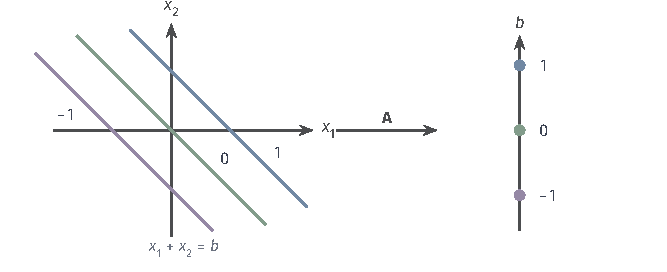
\includegraphics[width=112mm]{figures/00-shared/mathematical-preliminaries-upper/02-linear-spaces/tikz/comprehension-additions/linear-nullspace-fibers.pdf}
  \caption{同一输出对应的整组输入。对$\bm A=(1,1)$，蓝、绿、紫直线分别满足
  $x_1+x_2=1,0,-1$；右侧同色点是各直线的输出。绿色直线是$\ker\bm A$，
  其余直线是它的平移。把一整条直线归为一类后，才得到与可达输出的一一对应。}
  \label{fig:vol1-add-linear-nullspace-fibers}
\end{figure}

解集有多大，由零空间的维数决定。$\dim\operatorname{null}(\bm A)=d-r$，取零空间的一组基$\bm n_1,\ldots,\bm n_{d-r}$，
全部解可写成$\bm x_0+t_1\bm n_1+\cdots+t_{d-r}\bm n_{d-r}$，其中$t_1,\ldots,t_{d-r}$任意取值，
所以解集有$d-r$个自由参数。上例中$d=2$、$r=1$，自由参数只有$t$一个。

\paragraph{特解与零空间基的计算}

这一描述需要两样东西：一个特解和零空间的一组基。二者都可以从消元得到的阶梯形读出
（第~\ref{sec:ls-direct-methods}节）。主元所在的列对应主元变量，其余未知量称为自由变量，共$d-r$个。
把全部自由变量取零，回代解出主元变量，就得到一个特解；把右端换成零，令某一个自由变量取$1$、其余取零，
回代得到零空间中的一个向量，依次对每个自由变量这样做，得到的$d-r$个向量线性无关，构成零空间的一组基。
下面的例子按这一步骤计算。

\begin{example}[从阶梯形读出特解与零空间的基]
\label{ex:ls-particular-null-basis}
解
\[
 \begin{bmatrix}1&2&1\\2&4&3\end{bmatrix}\bm x=\begin{bmatrix}4\\9\end{bmatrix}.
\]
第二行减去第一行的$2$倍，得阶梯形
\[
 \begin{bmatrix}1&2&1\\0&0&1\end{bmatrix}\bm x=\begin{bmatrix}4\\1\end{bmatrix},
\]
即$x_3=1$。主元在第一、三列，$x_2$是自由变量，$r=2$、$d-r=1$。取$x_2=0$，
回代$x_1=4-2x_2-x_3=3$，得特解$\bm x_0=(3,0,1)^\top$。右端换成零并取$x_2=1$，得$x_3=0$、$x_1=-2$，
零空间由$\bm n=(-2,1,0)^\top$张成。所以全部解为
\[
\begin{gathered}
\bm x=(3-2t,\,t,\,1)^\top\\
t\in\mathbb R .
\end{gathered}
\]
代回可验$\bm A\bm x_0=(4,9)^\top$、$\bm A\bm n=\bm0$。
\end{example}

\subsection{相容方程的最小范数解}

方程本身给出的是整个仿射空间$\bm x_0+\operatorname{null}(\bm A)$，并不指定其中哪一个点。
若要报告一个确定的答案，必须另加准则。
最常用的准则是取欧氏范数最小的解，几何上就是在仿射空间中找离原点最近的点。

准则需要事先声明，因为不同准则选出的点不同：换一个内积，离原点“最近”的点一般也会改变。
示例~\ref{ex:ls-particular-null-basis}的特解$(3,0,1)^\top$也是一个合法的解，
只是它来自“自由变量取零”这一约定，换一种消元顺序就会得到另一个特解。

为求范数最小的点，把输入分成两部分：被$\bm A$消去的部分和真正决定输出的部分。
第一部分属于$\operatorname{null}(\bm A)$；第二部分应取在它的正交补中。
由定理~\ref{thm:ls-four-subspaces-orthogonality}，这个正交补就是行空间，$\operatorname{null}(\bm A)^\perp=\operatorname{range}(\bm A^\top)$，
输入空间有正交直和$\mathbb R^d=\operatorname{range}(\bm A^\top)\oplus\operatorname{null}(\bm A)$（式~\eqref{eq:ls-four-subspaces-decomposition}）：
$\operatorname{null}(\bm A)$是被消去的输入方向，$\operatorname{range}(\bm A^\top)$是真正影响输出的方向。

\paragraph{最小范数精确解的唯一性}

按输入空间的分解，每个解唯一写成$\bm x=\bm x_R+\bm x_N$，其中$\bm x_R\in\operatorname{range}(\bm A^\top)$，
$\bm x_N\in\operatorname{null}(\bm A)$。所有解共有同一个$\bm x_R$：若$\bm x'=\bm x'_R+\bm x'_N$是另一个解，
则$\bm x_R-\bm x'_R=(\bm x-\bm x')-(\bm x_N-\bm x'_N)$既在$\operatorname{range}(\bm A^\top)$中，
又是两个零空间向量之差，落在$\operatorname{null}(\bm A)$中；两个子空间互相正交，只交于零向量，故$\bm x_R=\bm x'_R$。
由于$\bm A\bm x_N=\bm0$，$\bm A\bm x_R=\bm A\bm x=\bm b$，$\bm x_R$本身也是解。两部分正交，勾股恒等式给出
\[
 \lVert\bm x\rVert_2^2=\lVert\bm x_R\rVert_2^2+\lVert\bm x_N\rVert_2^2\geq\lVert\bm x_R\rVert_2^2,
\]
等号当且仅当$\bm x_N=\bm0$。所以最小范数解存在且唯一，就是解集中落在$\operatorname{range}(\bm A^\top)$里的那一个。
用前面的直线方程核对这一刻画。

\begin{example}[直线$x_1+x_2=2$上的最小范数解]
\label{ex:ls-min-norm-line}
方程$x_1+x_2=2$的系数矩阵为$\bm A=(1,1)$，全部解为$(1+t,1-t)^\top$，$t\in\mathbb R$。它们的范数平方为
\[
 (1+t)^2+(1-t)^2=2+2t^2,
\]
在$t=0$时最小，所以最小范数解是$(1,1)^\top$。它正比于$\bm A^\top=(1,1)^\top$，确实落在$\operatorname{range}(\bm A^\top)$中。
\end{example}

\paragraph{最小范数解的计算}

这一刻画也给出计算方法。

设$\bm A$满行秩，要找的解形如$\bm x=\bm A^\top\bm w$，代入方程得
$\bm A\bm A^\top\bm w=\bm b$。$m$阶方阵$\bm A\bm A^\top$可逆：若$\bm A\bm A^\top\bm w=\bm0$，
则$\lVert\bm A^\top\bm w\rVert_2^2=\bm w^\top\bm A\bm A^\top\bm w=0$，即$\bm A^\top\bm w=\bm0$，
而$\bm A^\top$的$m$列线性无关，迫使$\bm w=\bm0$。于是最小范数解为
\[
 \bm x=\bm A^\top(\bm A\bm A^\top)^{-1}\bm b .
\]
实际计算时不形成逆矩阵：$\bm A\bm A^\top$对称正定，先用Cholesky分解解出$\bm w$，再算$\bm A^\top\bm w$。

\begin{example}[满行秩方程的最小范数解]
\label{ex:ls-min-norm-row-full-rank}
示例~\ref{ex:ls-particular-null-basis}的系数矩阵$\bm A=\left[\begin{smallmatrix}1&2&1\\2&4&3\end{smallmatrix}\right]$的秩为$2$，满行秩。计算
\[
 \bm A\bm A^\top=\begin{bmatrix}6&13\\13&29\end{bmatrix},
\]
解$\bm A\bm A^\top\bm w=(4,9)^\top$得$\bm w=(-1/5,2/5)^\top$，于是
\[
 \bm x=\bm A^\top\bm w=(3/5,\,6/5,\,1)^\top .
\]
它是全部解$(3-2t,t,1)^\top$中$t=6/5$的那一个，与零空间方向$(-2,1,0)^\top$正交。
它的范数平方为$14/5$，小于特解$(3,0,1)^\top$的范数平方$10$。
\end{example}

矩阵$\bm A^\top(\bm A\bm A^\top)^{-1}$从右边乘$\bm A$得到单位矩阵，是第~\ref{sec:prelim-inverse-matrices}节介绍过的右逆中的一个。
右逆不唯一，其他右逆给出的一般不是最小范数解。

\begin{example}[反例：其他右逆不给出最小范数解]
\label{ex:ls-other-right-inverse}
取$\bm A=(1,1)$。右逆$\bm A^\top(\bm A\bm A^\top)^{-1}=(1/2,1/2)^\top$把$b$送到最小范数解$(b/2,b/2)^\top$，范数为$|b|/\sqrt2$。
$(1,0)^\top$也满足$\bm A(1,0)^\top=1$，是另一个右逆；它把$b$送到$(b,0)^\top$。这也是方程的解，
但范数为$|b|$，$b\neq0$时大于最小范数。
\end{example}

形成$\bm A\bm A^\top$会把各行之间接近线性相关的程度放大（第~\ref{sec:ls-normal-equations-method}节对$\bm A^\top\bm A$说明了同样的现象）。
更可靠的做法是对$\bm A^\top$作第~\ref{chap:normed-inner-product-spaces}章的经济型QR分解~\eqref{eq:ls-qr-factorization}，
$\bm A^\top=\bm Q\bm R$，$\bm Q$是$d\times m$矩阵，$\bm R$是$m$阶可逆上三角矩阵。
最小范数解落在$\operatorname{range}(\bm A^\top)=\operatorname{range}(\bm Q)$中，可写成$\bm x=\bm Q\bm w$。
代入方程，$\bm A\bm x=\bm R^\top\bm Q^\top\bm Q\bm w=\bm R^\top\bm w=\bm b$，
这是下三角方程，前代即得$\bm w$。所得的解与上面的公式相同，但不形成$\bm A\bm A^\top$；
QR分解怎样稳定地计算，见第~\ref{sec:ls-orthogonalization-qr}节。

$\bm A$不满行秩时，有些方程可以由其他方程组合出来，$\bm A\bm A^\top$不可逆，上面的公式不能直接使用。
方程相容时，可以先删去这些多余的方程，化为满行秩的情形；要把最小范数解写成一个矩阵作用于$\bm b$，
则需要第~\ref{sec:ls-pseudoinverse}节的伪逆。

至此，无穷多解的情形已经回答：全部解是一个特解加零空间，二者都可由消元读出；
若只报告一个解，须声明准则，欧氏范数最小的解是解集中唯一落在$\operatorname{range}(\bm A^\top)$里的点，
满行秩时可由$\bm A\bm A^\top$的Cholesky分解或$\bm A^\top$的QR分解算出。
\section{直接求解}
\label{sec:ls-direct-methods}
\label{sec:linear-algebra-direct-exact}
\label{sec:matrix-analysis-stable-solvers}

本节讨论最常见的唯一解情形：$\bm A$是可逆方阵，对每个右端恰有一解。
超定而满列秩的方程在相容时也有唯一解，但判断它是否相容本身就要比较$\bm b$与列空间，
这与最小二乘的计算是同一件事，放到第~\ref{sec:ls-qr-method}节一并处理。

知道解唯一存在，还要把它算出来。三角方程最容易解：上三角方程的最后一个方程只含最后一个未知量，
解出后代入倒数第二个方程，又只剩一个未知量，如此从后向前逐个求出。

本节的方法都把一般方程化成三角方程，或化成规模更小的方程，在有限步内得到精确算术下的精确解，称为直接法。
它们需要整体读取矩阵并存储分解因子，适合矩阵规模可控、或同一矩阵要配多个右端的情形。

不同方法利用不同的矩阵结构。我们从一般方阵的消元出发，得到LU分解；对称正定矩阵可以省去一半运算，
得到Cholesky分解；对称但不定的矩阵用LDL$^{\top}$分解；具有分块结构或只作低秩修改的矩阵，
可以把大方程化成小方程。用正交变换化三角的QR分解同样能解方程，它与最小二乘一起在第~\ref{sec:ls-qr-method}节讨论。
最后把这些方法的适用条件和代价并列比较，并说明算出的解怎样核验。

\subsection{消元、主元与LU分解}

对一般可逆的$d$阶系数矩阵，目标是从$\bm A\bm x=\bm b$得到唯一的$\bm x$。直接写成$\bm A^{-1}\bm b$还没有说明怎样计算。消元的想法是同时变换系数和右端，把每个方程依赖的未知量逐渐减少，直到可以回代；LU分解则保存这些变换，以便换一个右端时继续使用。

高斯消元用一个方程的倍数去消另一个方程中的未知量。三种行变换——把某行的倍数加到另一行、交换两行、
某行乘非零常数——都可以逆转，因而不改变解集。先看一个二阶的例子。

\begin{example}[二阶方程的消元]
\label{ex:ls-elimination-two-by-two}
解
\[
 \begin{bmatrix}2&1\\4&3\end{bmatrix}\bm x=\begin{bmatrix}1\\3\end{bmatrix},
\]
即$2x_1+x_2=1$、$4x_1+3x_2=3$。第二个方程减去第一个方程的$2$倍，消去$x_1$，得$x_2=1$。
代回第一个方程，$2x_1+1=1$，得$x_1=0$。所以唯一解是$\bm x=(0,1)^\top$。
\end{example}

\paragraph{消元乘子与LU因子}

阶数较高时，消元按列进行，每一步把一列主对角线以下的元素全部消成零。下面的例子显示，
记下每一步所用的倍数，就得到矩阵的一个乘积分解。

\begin{example}[三阶消元与LU分解]
\label{ex:ls-lu-three-by-three}
考虑方程
\[
 \bm A\bm x=\begin{bmatrix}2&1&1\\4&3&3\\8&7&9\end{bmatrix}\bm x
 =\begin{bmatrix}3\\7\\19\end{bmatrix},
\]
先只对系数矩阵$\bm A$消元。第一步以$a_{1,1}=2$为主元，即用来做除数的元素。
第二行减去第一行的$l_{2,1}=4/2=2$倍，变为$(0,1,1)$；第三行减去第一行的$l_{3,1}=8/2=4$倍，变为$(0,3,5)$。
第二步以新的$(2,2)$元$1$为主元，第三行减去第二行的$l_{3,2}=3/1=3$倍，变为$(0,0,2)$。
消元结束时剩下上三角矩阵$\bm U$，三个乘子按位置填进单位下三角矩阵$\bm L$：
\[
\begin{gathered}
\bm L=\begin{bmatrix}1&0&0\\2&1&0\\4&3&1\end{bmatrix}\\
\bm U=\begin{bmatrix}2&1&1\\0&1&1\\0&0&2\end{bmatrix}.
\end{gathered}
\]
乘回可验$\bm L\bm U=\bm A$，例如$\bm L\bm U$的第三行是$4\cdot(2,1,1)+3\cdot(0,1,1)+(0,0,2)=(8,7,9)$。
\end{example}

图~\ref{fig:ls-lu-elimination-steps}画出这两步消元，以及乘子怎样按位置收集成$\bm L$。
乘回之所以能复原$\bm A$，是因为消元过程可以倒过来读。$\bm U$的第$i$行，是$\bm A$的第$i$行减去
若干个已经处理好的行（即$\bm U$的前$i-1$行）的倍数得到的，倍数就是乘子$l_{i,k}$：
\[
 \bm U_{i,:}=\bm A_{i,:}-\sum_{k<i}l_{i,k}\bm U_{k,:}
 \quad\Longrightarrow\quad
 \bm A_{i,:}=\sum_{k<i}l_{i,k}\bm U_{k,:}+1\cdot\bm U_{i,:}.
\]
右式说明$\bm A$的第$i$行是$\bm U$各行以$(l_{i,1},\ldots,l_{i,i-1},1,0,\ldots,0)$为系数的组合，
这正是$\bm L\bm U$的第$i$行。因此只要消元中不出现零主元，就有$\bm A=\bm L\bm U$，
其中$\bm L$是对角元为$1$的下三角矩阵，$\bm U$是上三角矩阵，称为LU分解。

有了分解，$\bm A\bm x=\bm b$就是$\bm L(\bm U\bm x)=\bm b$。

令$\bm z=\bm U\bm x$，先从前向后解下三角方程
$\bm L\bm z=\bm b$（前代），再从后向前解上三角方程$\bm U\bm x=\bm z$（回代）：
\begin{equation}
\begin{gathered}
z_i=b_i-\sum_{j<i}l_{i,j}z_j\\
x_i=\frac{z_i-\sum_{j>i}u_{i,j}x_j}{u_{i,i}}.
\end{gathered}
\end{equation}
下面用这两个公式完成示例~\ref{ex:ls-lu-three-by-three}的求解。

\begin{example}[用LU因子前代与回代]
\label{ex:ls-lu-forward-back}
沿用示例~\ref{ex:ls-lu-three-by-three}的因子$\bm L,\bm U$与右端$\bm b=(3,7,19)^\top$。前代解$\bm L\bm z=\bm b$：
\[
 \begin{gathered}
z_1=3\\
z_2=7-2\cdot3=1\\
z_3=19-4\cdot3-3\cdot1=4.
 \end{gathered}
\]
回代解$\bm U\bm x=\bm z$：
\[
 \begin{gathered}
x_3=\frac42=2\\
x_2=\frac{1-1\cdot x_3}{1}=-1,
 \end{gathered}
\]
\[
 x_1=\frac{3-1\cdot x_2-1\cdot x_3}{2}=1.
\]
代回原方程，$\bm A(1,-1,2)^\top=(3,7,19)^\top$，所以$\bm x=(1,-1,2)^\top$是方程的解。
\end{example}

前代算出的$\bm z$，正是消元过程对右端做同样变换的结果：例如$z_2=7-2\cdot3$，
就是第二行减去第一行的$2$倍时右端的变化。
\begin{figure}[!htb]
  \centering
  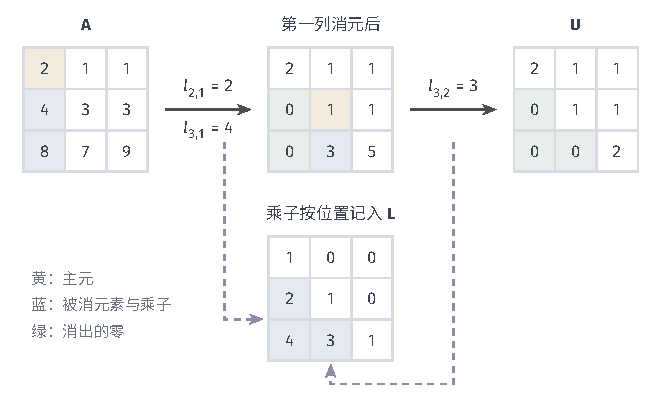
\includegraphics[width=112mm]{figures/00-shared/mathematical-preliminaries-upper/02-linear-spaces/tikz/comprehension-additions/linear-lu-elimination-steps.pdf}
  \caption{三阶矩阵的消元与LU因子。左起依次是$\bm A$、消去第一列后的矩阵与$\bm U$；
  黄色是当前主元，蓝色是待消去的元素，绿色是消出的零。箭头上的乘子等于被消元素除以主元，
  下方按原位置收集成单位下三角因子$\bm L$，满足$\bm L\bm U=\bm A$。}
  \label{fig:ls-lu-elimination-steps}
\end{figure}

\paragraph{选主元}

上面的做法要求每一步的主元不为零。可逆矩阵也可能在主元位置出现零，例如
$\left[\begin{smallmatrix}0&1\\1&1\end{smallmatrix}\right]$的$(1,1)$元为零，无法用它做除数；
交换两行后，以$1$为主元即可继续。主元不为零但很小时，问题同样存在，只是在浮点计算中才暴露出来。
下面的例子用只保留三位有效数字的算术显示这一点。

\begin{example}[小主元与行交换]
\label{ex:ls-partial-pivoting}
解$\left[\begin{smallmatrix}10^{-4}&1\\1&1\end{smallmatrix}\right]\bm x=(1,2)^\top$，
精确解为$x_1=1/(1-10^{-4})\approx1.0001$、$x_2=2-x_1\approx0.9999$。设每步运算结果
只保留三位有效数字（教学设定）。

不交换时，以$10^{-4}$为主元，乘子$l_{2,1}=10^4$。消元后右下角系数
$1-10^4=-9999$舍入为$-1.00\times10^4$，右端$2-10^4=-9998$也舍入为
$-1.00\times10^4$，得$x_2=1.00$，回代$x_1=(1-1.00)/10^{-4}=0$，第一分量完全错误：
大乘子把第二行原有的“$1$”和“$2$”淹没在$10^4$量级中。

先交换两行，以$1$为主元，乘子$l_{2,1}=10^{-4}$。消元后右下角系数$1-10^{-4}$与右端$1-2\times10^{-4}$
都舍入为$1.00$，得$x_2=1.00$，回代$x_1=2-1.00=1.00$，两分量在三位精度下都正确。
两种做法在精确算术中给出同一个解，区别只在乘子大小。
\end{example}

示例~\ref{ex:ls-partial-pivoting}说明，主元比同列其他元素小得多时，乘子会很大，舍入误差随之被放大。
因此第$k$步先在第$k$列尚未处理的元素中选绝对值最大的一个，把它所在的行换到主元位置，再消元。
这种做法称为部分主元，它保证每个乘子满足$|l_{i,k}|\leq1$。把全部行交换累计成置换矩阵$\bm P$，
得到带部分主元的LU分解
\begin{equation}
 \bm P\bm A=\bm L\bm U,
 \label{eq:matrix-analysis-palu}
\end{equation}
求解时先把右端按同样的方式重排，依次解$\bm L\bm z=\bm P\bm b$与$\bm U\bm x=\bm z$。

从输入到输出，带主元的算法可以按以下次序执行。
\begin{enumerate}
 \item 复制$\bm A$为工作矩阵，令$\bm P=\bm I$。对$k=1,\ldots,d-1$，在当前第$k$列的第$k$至$d$行选绝对值最大的主元，并交换相应两行。同步交换$\bm P$的两行，以及$\bm L$前$k-1$列中已记录的两行乘子。
 \item 对$i=k+1,\ldots,d$，用当前元素计算$l_{i,k}=a_{i,k}^{\mathrm{work}}/a_{k,k}^{\mathrm{work}}$，并对$j=k+1,\ldots,d$更新$a_{i,j}^{\mathrm{work}}\leftarrow a_{i,j}^{\mathrm{work}}-l_{i,k}a_{k,j}^{\mathrm{work}}$。处理完全部列后，上三角部分就是$\bm U$，乘子与单位对角线组成$\bm L$。
 \item 计算$\bm c=\bm P\bm b$，前代求$\bm z$，再回代求$\bm x$。最后计算$\bm b-\bm A\bm x$，其中使用的是原始系数与右端。
\end{enumerate}
这里主元选择和更新都使用工作矩阵的当前值，不再使用最初的$a_{i,j}$。在唯一解假设下，每一步都能找到非零主元；失去这一条件时，需要按下面的秩亏情形处理。

行交换只改变方程的排列次序，不改变解集。若示例~\ref{ex:ls-lu-three-by-three}也用部分主元，
第一步会把含$8$的第三行换到顶部，得到另一组$\bm P,\bm L,\bm U$，解不变。

行交换不会把奇异矩阵变成可逆矩阵。若某一步在精确算术下，当前列尚未处理的元素全为零，找不到非零主元，
说明这一列是前面主元列的组合，矩阵秩亏。这时跳过该列，继续处理下一列，最后得到阶梯形，非零主元的个数就是秩。

这样，消元同时回答了第~\ref{sec:ls-solution-cases}节的问题。
在阶梯形中，若某行左边全为零而右端非零，即出现$0=c\neq0$的矛盾行，方程不相容，这与增广矩阵的秩判据一致；
若没有矛盾行，把不对应主元的未知量（自由变量）取零，回代即得一个特解，其余解沿零空间展开，
具体做法见第~\ref{sec:ls-select-among-solutions}节。

浮点计算中，一个很小的主元并不能证明矩阵精确奇异：代数上的奇异（主元恰为零）与数值上的接近奇异
（主元很小但非零）是两回事，后者用数值秩描述，见第~\ref{sec:ls-numerical-sensitivity}节。

\paragraph{代价、复用与填充}

稠密$d\times d$矩阵的LU分解约需$2d^3/3$次浮点运算，$\bm L$与$\bm U$可以覆盖原矩阵存放，存储为$O(d^2)$。
分解完成后，每个右端只需前代与回代各一次，运算量为$O(d^2)$。所以同一个$\bm A$配多个右端$\bm b_j$时，
分解只做一次，此后每列只付$O(d^2)$的代价。复用的前提是矩阵不变；矩阵元素一旦改变，旧的$\bm L\bm U$
不再等于新的$\bm P\bm A$，必须重新分解，或改用后文的低秩更新。

稀疏矩阵的情形更微妙。消元会在原来为零的位置产生非零元，称为\term{填充}（fill-in），
使原本稀疏的因子变得接近稠密。填充的多少取决于消元顺序，下面的箭头形矩阵说明这一点。

\begin{example}[箭头形矩阵的填充]
\label{ex:ls-arrow-fill-in}
考虑一个$5\times5$矩阵，其中一个变量与其余全部变量耦合，其余变量彼此不耦合，
非零元只在对角线和这个变量对应的行与列上。

若先消去这个变量，要从其余每一行减去它所在行的倍数，而这一行在所有列上都有非零元，
所以剩下的$4\times4$块全部变成非零：原来只有$4$个对角非零元，现在有$16$个，新增的$12$个都是填充。
若把它排到最后，消去前四个变量时，每一步只改动右下角那一个元素，不产生任何填充。

推广到$n$阶，前一种顺序使因子变为稠密，需存约$n^2$个元素，分解约需$O(n^3)$次运算；
后一种只需原有的$3n-2$个元素和$O(n)$次运算。
\end{example}

图~\ref{fig:ls-sparse-fill-in-ordering}并置了两种顺序。矩阵和解都相同，代价却随顺序相差悬殊，
所以稀疏直接法先选消元顺序、再作分解，其代价也不能只按原始非零元数估计。
\begin{figure}[!htb]
  \centering
  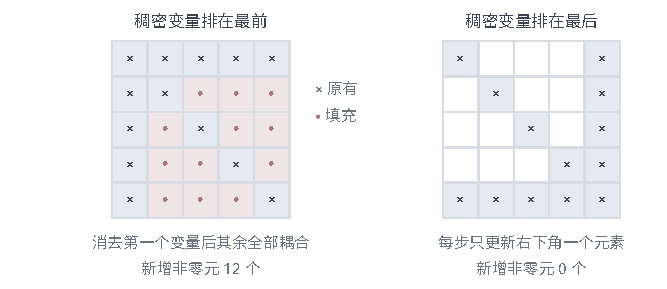
\includegraphics[width=112mm]{figures/00-shared/mathematical-preliminaries-upper/02-linear-spaces/tikz/comprehension-additions/linear-sparse-fill-in-ordering.pdf}
  \caption{消元顺序决定填充。同一个“箭头形”矩阵：左图把与全部变量耦合的变量排在最前，
  消去它后其余位置全部变为非零（红点为填充）；右图把它排在最后，因子保持原有稀疏结构。
  蓝格是原矩阵的非零元。}
  \label{fig:ls-sparse-fill-in-ordering}
\end{figure}

\subsection{正定方程与Cholesky分解}

很多方程的系数矩阵是对称正定的，例如第~\ref{sec:ls-least-squares}节满列秩时的$\bm A^\top\bm A$。
对这类矩阵，LU分解有两处浪费：$\bm U$与$\bm L$实际上携带同样的信息（$\bm U$的第$i$行是$\bm L^\top$的第$i$行乘以第$i$个主元），却要分别计算和存储；
部分主元的行交换会破坏对称性，而对称正定矩阵其实不需要交换。下面说明，对称正定矩阵可以写成
$\bm L\bm L^\top$，只算一个三角因子，并且不必选主元。

设$\bm A=\bm A^\top\succ0$。把第一行、第一列与其余部分分开，也把待求的下三角因子同样分块：
\[
\begin{gathered}
\bm A=\begin{bmatrix}a_{1,1}&\bm a^\top\\\bm a&\bm A_{22}\end{bmatrix}\\
\bm L=\begin{bmatrix}l_{1,1}&\bm0\\\bm l&\bm L_{22}\end{bmatrix}\\
\bm L\bm L^\top=\begin{bmatrix}l_{1,1}^2&l_{1,1}\bm l^\top\\ l_{1,1}\bm l&\bm l\bm l^\top+\bm L_{22}\bm L_{22}^\top\end{bmatrix}.
\end{gathered}
\]
令$\bm L\bm L^\top=\bm A$并逐块比较：左上角要求$l_{1,1}^2=a_{1,1}$。正定性给出
$a_{1,1}=\bm e_1^\top\bm A\bm e_1>0$，故可取$l_{1,1}=\sqrt{a_{1,1}}>0$。左下角要求$\bm l=\bm a/l_{1,1}$。
右下角要求
\[
 \bm L_{22}\bm L_{22}^\top=\bm A_{22}-\bm l\bm l^\top=\bm A_{22}-\frac{\bm a\bm a^\top}{a_{1,1}},
\]
问题化为对低一阶的矩阵$\bm A_{22}-\bm a\bm a^\top/a_{1,1}$做同样的分解。

这个剩余矩阵仍然对称正定。对任意非零$\bm u$，取$\bm x=(-\bm a^\top\bm u/a_{1,1},\,\bm u)$，它非零，展开可得
$\bm x^\top\bm A\bm x=\bm u^\top(\bm A_{22}-\bm a\bm a^\top/a_{1,1})\bm u$，而左边为正。
右边正是对第一个变量配方后剩下的二次型。于是同样的论证可以一阶一阶做下去，每一步开方的数都严格为正。
定理~\ref{thm:ls-gram-factor}用同样的配方归纳证明了正定矩阵可写成$\bm L^\top\bm L$的形式，
那里的上三角因子就是这里的$\bm L^\top$；这里把同一构造落实为逐列计算的算法。

\paragraph{Cholesky因子的逐列构造}

总结起来，对称正定矩阵$\bm A$存在唯一的对角元为正的下三角矩阵$\bm L$，使
\begin{equation}
 \bm A=\bm L\bm L^\top,
 \label{eq:matrix-analysis-cholesky}
\end{equation}
称为\term{Cholesky分解}（Cholesky decomposition）。上面的分块递推展开成逐元素的形式，就是按列计算
\begin{equation}
\begin{gathered}
l_{j,j}=\sqrt{a_{j,j}-\sum_{k<j}l_{j,k}^2}\\
l_{i,j}=\frac{a_{i,j}-\sum_{k<j}l_{i,k}l_{j,k}}{l_{j,j}}\quad(i>j).
\end{gathered}
\end{equation}
两式都来自比较$\bm L\bm L^\top$与$\bm A$的元素：$\bm L\bm L^\top$的$(i,j)$元（$i\geq j$）是
$\sum_{k\leq j}l_{i,k}l_{j,k}$，其中$k<j$的项只含前面各列，已经算出；剩下的一项$l_{i,j}l_{j,j}$
（$i=j$时是$l_{j,j}^2$）便可解出。根号内的数是第$j$步配方后的剩余，正定性保证它严格为正。
唯一性也由此可见：每个元素都被唯一解出，只有开方有正负两种选择，约定对角元为正就排除了这一任意性。
下面按这两个公式算一个三阶的例子。

\begin{example}[逐列计算Cholesky因子]
\label{ex:ls-cholesky-three-by-three}
取对称矩阵
$\bm A=\left[\begin{smallmatrix}4&2&2\\2&5&3\\2&3&6\end{smallmatrix}\right]$。
第一列：$l_{1,1}=\sqrt4=2$，$l_{2,1}=2/2=1$，$l_{3,1}=2/2=1$。此时剩余矩阵为
\[
 \begin{bmatrix}5&3\\3&6\end{bmatrix}-\begin{bmatrix}1&1\\1&1\end{bmatrix}
 =\begin{bmatrix}4&2\\2&5\end{bmatrix}.
\]
第二列：$l_{2,2}=\sqrt{5-l_{2,1}^2}=\sqrt4=2$，$l_{3,2}=(3-l_{3,1}l_{2,1})/l_{2,2}=(3-1)/2=1$。
第三列：$l_{3,3}=\sqrt{6-l_{3,1}^2-l_{3,2}^2}=\sqrt4=2$。于是
\[
 \bm L=\begin{bmatrix}2&0&0\\1&2&0\\1&1&2\end{bmatrix},
\]
乘回$\bm L\bm L^\top$逐项等于$\bm A$。三个根号内的数都是$4$，都为正。
\end{example}

在精确算术下，计算本身也是正定性的检验。若每一步根号内的数都为正，就得到可逆的$\bm L$，
于是对非零$\bm x$有$\bm x^\top\bm A\bm x=\lVert\bm L^\top\bm x\rVert_2^2>0$，$\bm A$正定；
反之，若某一步根号内出现零或负数，$\bm A$就不是正定的。示例~\ref{ex:ls-cholesky-three-by-three}的计算因此同时证明了$\bm A$正定。浮点运算中，接近零的配方剩余可能受到舍入影响，因此分解是否成功只能作为数值判断，还须结合误差尺度。

求解时，依次解$\bm L\bm z=\bm b$（前代，$z_i=(b_i-\sum_{j<i}l_{i,j}z_j)/l_{i,i}$）与
$\bm L^\top\bm x=\bm z$（回代，$x_i=(z_i-\sum_{j>i}l_{j,i}x_j)/l_{i,i}$）。

\begin{example}[用Cholesky因子求解]
\label{ex:ls-cholesky-solve}
沿用示例~\ref{ex:ls-cholesky-three-by-three}的$\bm A$与$\bm L$，取右端$\bm b=(8,10,11)^\top$。前代解$\bm L\bm z=\bm b$：
\[
 \begin{gathered}
z_1=\frac82=4\\
z_2=\frac{10-1\cdot4}{2}=3\\
z_3=\frac{11-1\cdot4-1\cdot3}{2}=2.
 \end{gathered}
\]
回代解$\bm L^\top\bm x=\bm z$：
\[
 \begin{gathered}
x_3=\frac22=1\\
x_2=\frac{3-1\cdot1}{2}=1\\
x_1=\frac{4-1\cdot1-1\cdot1}{2}=1.
 \end{gathered}
\]
代回可验$\bm A(1,1,1)^\top=(8,10,11)^\top$，所以$\bm x=(1,1,1)^\top$。
\end{example}

稠密情形的运算量约为$d^3/3$，是LU的一半；存储也只需一个三角因子，约$d^2/2$个元素。多个右端同样复用一次分解。

矩阵只是半正定时，某一步的配方剩余可能恰为零，后续除以$l_{j,j}$就无法进行。
这时不应随手给对角线加一个小常数让计算通过，那样解的已经是另一个方程。
应先分清原因：$\bm A$本身有零空间时，方程不再有唯一解，回到第~\ref{sec:ls-solution-cases}节判断它属于哪种情况；
剩余量只是因舍入而接近零时，属于数值问题，见第~\ref{sec:ls-numerical-sensitivity}节。
只有任务本身要求加入惩罚项时，才改解相应的正则化方程（第~\ref{sec:ls-regularized-ls}节）。

\subsection{对称不定方程与分块LDL分解}
\label{sec:ls-ldlt}

对称但不定的矩阵，既有使二次型为正的方向，也有使它为负的方向。前面已经说明，逐列计算成功就证明矩阵正定，
所以对不定矩阵，Cholesky的开方必定在某一步遇到非正的数。下面是最小的例子。

\begin{example}[反例：不定矩阵的Cholesky中断]
\label{ex:ls-cholesky-indefinite}
取$\bm A=\left[\begin{smallmatrix}1&2\\2&1\end{smallmatrix}\right]$。它对称，$\det\bm A=-3\neq0$，所以可逆；
但$\bm x=(1,-1)^\top$给出$\bm x^\top\bm A\bm x=1-4+1=-2<0$，$\bm A$不定。按Cholesky的逐列公式，
第一列得$l_{1,1}=1$、$l_{2,1}=2$，第二列要求
\[
 l_{2,2}=\sqrt{a_{2,2}-l_{2,1}^2}=\sqrt{1-2^2}=\sqrt{-3},
\]
在实数中无法进行。
\end{example}

我们仍想利用对称性，只算一个三角因子。办法是不开方，把每一步的主元单独放进对角矩阵$\bm D$，负号就留在$\bm D$里。

\paragraph{LDL$^{\top}$因子的形成}

仍以示例~\ref{ex:ls-cholesky-indefinite}的矩阵为例，看不开方时消元记录下什么。

\begin{example}[二阶不定矩阵的LDL$^{\top}$分解]
\label{ex:ls-ldlt-two-by-two}
对$\bm A=\left[\begin{smallmatrix}1&2\\2&1\end{smallmatrix}\right]$，以$a_{1,1}=1$为主元，乘子$l_{2,1}=2/1=2$，
消元后剩余系数为$1-2\cdot2=-3$。把乘子放进单位下三角矩阵，把两个主元$1$与$-3$放进对角矩阵，得
\[
 \bm A=\begin{bmatrix}1&0\\2&1\end{bmatrix}
 \begin{bmatrix}1&0\\0&-3\end{bmatrix}
 \begin{bmatrix}1&2\\0&1\end{bmatrix}=\bm L\bm D\bm L^\top .
\]
乘回可验等式成立。剩余系数$-3$原样保留在$\bm D$中，不需要开方。
\end{example}

这就是LDL$^{\top}$分解的基本形式：$\bm L$是单位下三角矩阵，$\bm D$是对角矩阵。

只用一阶主元并不总够，下面的矩阵就没有可用的一阶主元。

\begin{example}[反例：没有一阶主元的对称可逆矩阵]
\label{ex:ls-no-scalar-pivot}
取$\bm A=\left[\begin{smallmatrix}0&1\\1&0\end{smallmatrix}\right]$。$\det\bm A=-1\neq0$，所以$\bm A$可逆；
但两个对角元都是零，没有一个能作除数。若像LU那样交换两行，得到的是$\bm P\bm A=\bm L\bm U$形式的分解，
不再是对称的$\bm L\bm D\bm L^\top$。若对称地交换，即同时交换两行和对应的两列，结果仍是$\bm A$本身：
对称置换只重新排列对角元，而这里的对角元全为零。
\end{example}

所以解决办法有两条。一是对称地交换，矩阵仍然对称，对角元被重新排列；若其他位置有合适的对角元，
就可以把它换到主元位置。二是允许用$2\times2$的对称可逆块作主元，在对角元都不合适时必须这样做：
示例~\ref{ex:ls-no-scalar-pivot}的整个矩阵就是一个可逆的二阶块，直接把它放进$\bm D$即可。
一般地，把对称置换累计成$\bm P$，得到
\[
 \bm P\bm A\bm P^\top=\bm L\bm D\bm L^\top,
\]
其中$\bm L$单位下三角，$\bm D$由一阶与二阶对角块组成。

计算过程与LU相同，只是按块进行。把当前待处理的矩阵分块为
$\left[\begin{smallmatrix}\bm A_{11}&\bm A_{21}^\top\\\bm A_{21}&\bm A_{22}\end{smallmatrix}\right]$，
其中$\bm A_{11}$是选定的可逆一阶或二阶主元块。正如标量消元用乘子$l_{i,k}=a_{i,k}/a_{k,k}$，
块消元的乘子块是$\bm L_{21}=\bm A_{21}\bm A_{11}^{-1}$；从下面的块行中减去$\bm L_{21}$乘主元块行，
左下块变成零，右下块变成
\[
 \bm A_{22}-\bm L_{21}\bm A_{21}^\top=\bm A_{22}-\bm A_{21}\bm A_{11}^{-1}\bm A_{21}^\top ,
\]
它仍是对称矩阵，对它重复同样的过程。$\bm L$收集各步的乘子块，$\bm D$收集各步的主元块。
每一步都可以把$\bm L\bm D\bm L^\top$乘回，核对它是否等于置换后的矩阵。

求解时先把右端按$\bm P$重排，再依次解下三角方程$\bm L\bm z=\bm P\bm b$、
块对角方程$\bm D\bm y=\bm z$与上三角方程$\bm L^\top\bm w=\bm y$，最后令$\bm x=\bm P^\top\bm w$还原次序。
其中块对角方程逐块求解：一阶块$d$直接得$y=z/d$；二阶块
$\left[\begin{smallmatrix}d_{11}&d_{12}\\d_{12}&d_{22}\end{smallmatrix}\right]$
的行列式$\Delta=d_{11}d_{22}-d_{12}^2$因主元块可逆而非零，由二阶逆矩阵公式得
\begin{equation}
\begin{gathered}
y_1=\frac{d_{22}z_1-d_{12}z_2}{\Delta}\\
y_2=\frac{d_{11}z_2-d_{12}z_1}{\Delta}.
\end{gathered}
\end{equation}
示例~\ref{ex:ls-no-scalar-pivot}的二阶块有$\Delta=-1$，代入得$y_1=z_2$、$y_2=z_1$，
两个未知量一次解出。与Cholesky相比，这一求解过程只是在两次三角求解之间插入了块对角求解，并多了置换与还原；
运算量同样约为$d^3/3$。

例如给示例~\ref{ex:ls-ldlt-two-by-two}配上右端$\bm b=(3,3)^\top$，此时无需置换。前代$\bm L\bm z=\bm b$得$\bm z=(3,-3)^\top$；块对角求解$\bm D\bm y=\bm z$得$\bm y=(3,1)^\top$；最后回代$\bm L^\top\bm x=\bm y$得$\bm x=(1,1)^\top$。代入原来的不定矩阵，得到$\bm A\bm x=(3,3)^\top$。负主元只改变中间方程的系数，并不妨碍求解。

最后要分清$\bm D$中的两种情况。负的对角元或不定的二阶块表示矩阵有负方向，但它们可逆，
方程照样唯一可解；零块则表示矩阵奇异，不能当作可逆块做除法，需要回到第~\ref{sec:ls-solution-cases}节重新判断解的情况。

\subsection{分块消元与Schur补}
\label{sec:matrix-analysis-blocks-updates}

LDL$^{\top}$分解中的块消元有更广的用途。若未知量可以自然地分成两组，而且消去其中一组很便宜，
就可以先消去它，只解剩下那组未知量满足的较小方程。先看每组只有一个未知量的最小例子。

\begin{example}[二阶方程的分块消元]
\label{ex:ls-block-elimination-two-by-two}
解$\left[\begin{smallmatrix}2&1\\1&2\end{smallmatrix}\right](x_1,x_2)^\top=(1,3)^\top$。
第一个方程$2x_1+x_2=1$给出$x_1=(1-x_2)/2$。代入第二个方程$x_1+2x_2=3$，得
\[
\begin{gathered}
\frac{1-x_2}{2}+2x_2=3\\
\text{即}\qquad \frac32x_2=3-\frac12=\frac52,
\end{gathered}
\]
故$x_2=5/3$，回代得$x_1=(1-5/3)/2=-1/3$。核验：$2(-1/3)+5/3=1$，$(-1/3)+2(5/3)=3$。
消去$x_1$后，$x_2$的系数从$2$变成$2-1\cdot\tfrac12\cdot1=\tfrac32$，右端从$3$变成$3-1\cdot\tfrac12\cdot1=\tfrac52$。
\end{example}

图~\ref{fig:ls-schur-block-elimination}把这两步并置。下面把标量换成块，看系数与右端的这两处变化在一般情形下是什么。

\begin{figure*}[htbp]
  \centering
  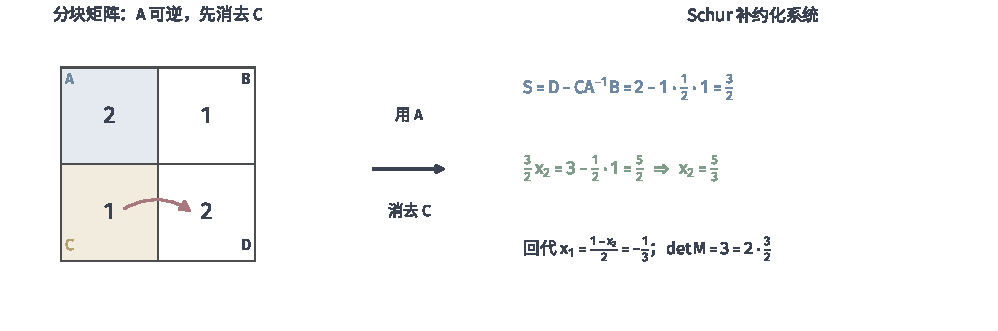
\includegraphics[width=168.998mm]{figures/00-shared/mathematical-preliminaries-upper/02-linear-spaces/matplotlib/ls-schur-block-elimination/ls-schur-block-elimination.pdf}
  \caption{Schur 补的 2×2 分块消元。左：$\bm M=\left[\begin{smallmatrix}2&1\\1&2\end{smallmatrix}\right]$
  按左上块$\bm A=2$分块，先由第一行表出$x_1=(1-x_2)/2$；右：代入第二行后右下角残留
  Schur补$\bm S=3/2$，约化得$x_2=5/3$、回代$x_1=-1/3$，且$\det\bm M=2\cdot3/2=3$。
  解析式教学构造。}
  \label{fig:ls-schur-block-elimination}
\end{figure*}

\paragraph{Schur补与约化系统}

这里仍然求解同一个$\bm A\bm x=\bm b$问题，只是把系数、未知量和右端各分成两组。为沿用常见的块公式，下面临时把整体系数记为$\bm M$，把它的四个块记为$\bm A,\bm B,\bm C,\bm D$；整体未知量和右端分别是$(\bm x^\top,\bm y^\top)^\top$与$(\bm f^\top,\bm g^\top)^\top$。这些块由原输入分割得到，并不是新的待估参数。

设分块方程为
\[
 \begin{bmatrix}\bm A&\bm B\\\bm C&\bm D\end{bmatrix}
 \begin{bmatrix}\bm x\\\bm y\end{bmatrix}
 =\begin{bmatrix}\bm f\\\bm g\end{bmatrix},
\]
系数矩阵记为$\bm M$，其中$\bm A\in\mathbb R^{p\times p}$可逆。第一组方程$\bm A\bm x+\bm B\bm y=\bm f$
给出$\bm x=\bm A^{-1}(\bm f-\bm B\bm y)$；代入第二组$\bm C\bm x+\bm D\bm y=\bm g$，得
$\bm C\bm A^{-1}\bm f-\bm C\bm A^{-1}\bm B\bm y+\bm D\bm y=\bm g$。整理后，$\bm y$满足
\begin{equation}
\begin{gathered}
\bm S\bm y=\bm g-\bm C\bm A^{-1}\bm f\\
\bm S=\bm D-\bm C\bm A^{-1}\bm B.
\end{gathered}
\label{eq:matrix-analysis-schur-complement}
\end{equation}
矩阵$\bm S$称为$\bm A$在$\bm M$中的\term{Schur补}（Schur complement），方程~\eqref{eq:matrix-analysis-schur-complement}
称为约化系统。

若要据此编写求解过程，输入四个块与两个右端后，先分解被消去的块$\bm A$，复用其因子解
\[
 \bm A\bm Z=\bm B,\qquad \bm A\bm u=\bm f.
\]
再形成$\bm S=\bm D-\bm C\bm Z$及$\bm h=\bm g-\bm C\bm u$，解小方程$\bm S\bm y=\bm h$，最后恢复$\bm x=\bm u-\bm Z\bm y$。输出是两组未知量合并后的向量；若只停在Schur补$\bm S$，还没有完成原问题的求解。
\label{def:matrix-analysis-schur-complement}
示例~\ref{ex:ls-block-elimination-two-by-two}相当于取$\bm A=2$、$\bm B=\bm C=1$、$\bm D=2$、$\bm f=1$、$\bm g=3$，
此时$\bm S=2-1/2=3/2$，约化系统的右端为$3-1/2=5/2$，与那里算出的系数和右端一致。
Cholesky每一步的剩余矩阵$\bm A_{22}-\bm a\bm a^\top/a_{1,1}$，以及LDL$^{\top}$每一步的右下块，都是这样的Schur补。

同一过程写成矩阵乘法，是左乘一个单位块下三角矩阵，消去左下块：
\[
 \begin{bmatrix}\bm I&\bm0\\-\bm C\bm A^{-1}&\bm I\end{bmatrix}
 \begin{bmatrix}\bm A&\bm B\\\bm C&\bm D\end{bmatrix}
 =\begin{bmatrix}\bm A&\bm B\\\bm0&\bm S\end{bmatrix}.
\]
左边第一个因子的行列式为$1$，右边是块上三角矩阵，所以$\det\bm M=\det\bm A\det\bm S$。
因此在$\bm A$可逆的前提下，$\bm M$可逆当且仅当$\bm S$可逆。示例~\ref{ex:ls-block-elimination-two-by-two}中$\det\bm M=3=2\cdot\tfrac32$。

计算时，先解约化系统得到$\bm y$，再回代$\bm x=\bm A^{-1}(\bm f-\bm B\bm y)$。其中凡是出现$\bm A^{-1}$的地方，
都通过对$\bm A$的分解求解来实现，例如$\bm A^{-1}\bm B$由解$\bm A\bm Z=\bm B$得到，不必先形成逆矩阵。
这种做法的典型来源是二部结构：少量全局未知量与大量局部未知量相连，局部未知量彼此之间不直接耦合。
这时$\bm A$是块对角的，消去局部块很便宜，只剩下全局未知量的小系统。

若需要整个逆矩阵，把上述消元过程对一般右端做完，可得块逆公式
\begin{equation}
 \bm M^{-1}=
 \begin{bmatrix}
  \bm A^{-1}+\bm A^{-1}\bm B\bm S^{-1}\bm C\bm A^{-1}
  &-\bm A^{-1}\bm B\bm S^{-1}\\
  -\bm S^{-1}\bm C\bm A^{-1}&\bm S^{-1}
 \end{bmatrix}.
 \label{eq:matrix-analysis-block-inverse}
\end{equation}

$\bm M$对称时$\bm C=\bm B^\top$，Schur补还能判断正定性。对二次型配方：
\begin{equation}
 \begin{aligned}
 &\begin{bmatrix}\bm x\\\bm y\end{bmatrix}^{\top}
 \bm M\begin{bmatrix}\bm x\\\bm y\end{bmatrix}\\
 &=\bm x^\top\bm A\bm x+2\bm x^\top\bm B\bm y+\bm y^\top\bm D\bm y\\
 &=(\bm x+\bm A^{-1}\bm B\bm y)^\top
 \bm A(\bm x+\bm A^{-1}\bm B\bm y)+\bm y^\top\bm S\bm y.
 \end{aligned}
\end{equation}
展开右边第一项即可验证第二个等号，它多出的$\bm y^\top\bm B^\top\bm A^{-1}\bm B\bm y$正好被$\bm S=\bm D-\bm B^\top\bm A^{-1}\bm B$
中的减项抵消。于是在$\bm A\succ0$时
\begin{equation}
 \bm M\succ0\quad\Longleftrightarrow\quad
 \bm D-\bm B^\top\bm A^{-1}\bm B\succ0.
 \label{eq:matrix-analysis-schur-positive-definite}
\end{equation}
必要性：对任意非零$\bm y$，取$\bm x=-\bm A^{-1}\bm B\bm y$使第一项为零，二次型只剩$\bm y^\top\bm S\bm y$，它必须为正。
充分性：两项都非负；若和为零，则$\bm y^\top\bm S\bm y=0$迫使$\bm y=\bm0$，再由第一项为零得$\bm x=\bm0$。
Cholesky中剩余矩阵保持正定，正是这一结论的特例。

$\bm A$奇异时上述公式不能使用。此时第一组方程$\bm A\bm x=\bm f-\bm B\bm y$本身未必有解，
对给定的$\bm y$，必须要求$\bm f-\bm B\bm y$落在$\operatorname{range}(\bm A)$中；
$\operatorname{range}(\bm B)\subseteq\operatorname{range}(\bm A)$加上$\bm f\in\operatorname{range}(\bm A)$可以保证这一条件对所有$\bm y$成立，却不是某个特定$\bm y$可解的必要条件。此外，$\bm A$的零空间还会给$\bm x$留下自由参数，须按第~\ref{sec:ls-solution-cases}节的判别另行处理。

\subsection{低秩更新与Woodbury公式}

另一类常见情形是：$\bm A$已经分解好，矩阵却改成了$\bm A+\bm U\bm C\bm V^\top$，其中
$\bm U,\bm V\in\mathbb R^{d\times k}$，$\bm C\in\mathbb R^{k\times k}$，$k$远小于$d$。
例如在最小二乘中增加或删除一条观测，系数矩阵就改变一个秩一项。这里的修改是精确的，不是近似。
重新分解需要$O(d^3)$次运算；能否借旧分解，只解一个$k$阶的小方程？

可以，办法是引入辅助未知量，把问题改写成分块方程，再用上面的Schur补。设$\bm C$可逆，要解
$(\bm A+\bm U\bm C\bm V^\top)\bm x=\bm b$。

令$\bm z=\bm C\bm V^\top\bm x\in\mathbb R^k$，原方程等价于
\[
 \begin{gathered}
\bm A\bm x+\bm U\bm z=\bm b\\
\bm V^\top\bm x-\bm C^{-1}\bm z=\bm0 .
 \end{gathered}
\]
按约化系统的做法消去$\bm x$：由第一式$\bm x=\bm A^{-1}(\bm b-\bm U\bm z)$，代入第二式得
$\bm V^\top\bm A^{-1}\bm b-\bm V^\top\bm A^{-1}\bm U\bm z-\bm C^{-1}\bm z=\bm0$，即
\[
 (\bm C^{-1}+\bm V^\top\bm A^{-1}\bm U)\bm z=\bm V^\top\bm A^{-1}\bm b .
\]
这是一个$k$阶方程。记它的系数矩阵为$\bm S=\bm C^{-1}+\bm V^\top\bm A^{-1}\bm U$，设其可逆，
则$\bm z=\bm S^{-1}\bm V^\top\bm A^{-1}\bm b$，代回得
$\bm x=\bm A^{-1}\bm b-\bm A^{-1}\bm U\bm S^{-1}\bm V^\top\bm A^{-1}\bm b$。
这对每个$\bm b$都成立，因此得到\term{Woodbury恒等式}
\begin{equation}
 (\bm A+\bm U\bm C\bm V^\top)^{-1}
 =\bm A^{-1}-\bm A^{-1}\bm U
 (\bm C^{-1}+\bm V^\top\bm A^{-1}\bm U)^{-1}
 \bm V^\top\bm A^{-1}.
 \label{eq:matrix-analysis-woodbury}
\end{equation}
计算时不必形成大矩阵的逆。先用旧因子解$\bm A\bm u=\bm b$与$\bm A\bm Z=\bm U$；再形成$\bm S=\bm C^{-1}+\bm V^\top\bm Z$和$\bm h=\bm V^\top\bm u$；求出$\bm S\bm z=\bm h$；最后返回$\bm x=\bm u-\bm Z\bm z$。若不希望显式形成$\bm C^{-1}$，则不必先形成$\bm S$，而是直接解$(\bm I+\bm C\bm V^\top\bm Z)\bm z=\bm C\bm h$。核验时使用更新后的系数$\bm A+\bm U\bm C\bm V^\top$。

由这些步骤可以直接计算代价：用旧分解解出$\bm A^{-1}\bm b$和$\bm A^{-1}\bm U$（共$k+1$个右端，每个右端一次前代、一次回代，代价$O(d^2)$），
形成并求解$k$阶小方程，再组合出$\bm x$，总代价为$O(kd^2+k^3)$。前提是$\bm A$可逆且已有分解，
小矩阵$\bm S$可逆；$\bm S$接近奇异时公式对误差敏感。最常用的是$\bm C=\bm I$，此时只要求
$\bm A$与$\bm I+\bm V^\top\bm A^{-1}\bm U$可逆，对矩形的$\bm U,\bm V$不需要任何逆。

$k=1$时$\bm U=\bm u$、$\bm V=\bm v$是向量，取$\bm C=1$，小方程变成标量方程，得到Sherman--Morrison公式
\[
\begin{gathered}
(\bm A+\bm u\bm v^\top)^{-1}
 =\bm A^{-1}-\frac{\bm A^{-1}\bm u\bm v^\top\bm A^{-1}}
 {1+\bm v^\top\bm A^{-1}\bm u}\\
1+\bm v^\top\bm A^{-1}\bm u\neq0 .
\end{gathered}
\]

行列式也有相应的公式。对上面的分块矩阵
$\left[\begin{smallmatrix}\bm A&\bm U\\\bm V^\top&-\bm C^{-1}\end{smallmatrix}\right]$，
先消左上块，行列式是$\det\bm A\det(-\bm S)$；改为先消右下块$-\bm C^{-1}$，对应的Schur补是
$\bm A-\bm U(-\bm C^{-1})^{-1}\bm V^\top=\bm A+\bm U\bm C\bm V^\top$，行列式是$\det(-\bm C^{-1})\det(\bm A+\bm U\bm C\bm V^\top)$。
两者相等，$k$阶矩阵前的负号各带出$(-1)^k$而抵消，得
$\det(\bm A+\bm U\bm C\bm V^\top)=\det\bm A\det\bm C\det\bm S$。

下面用一个二阶例子核对更新公式与行列式公式。

\begin{example}[秩一更新的求解]
\label{ex:ls-sherman-morrison-update}
取$\bm A=\operatorname{diag}(2,3)$、$\bm u=\bm v=(1,1)^\top$、$\bm b=(1,0)^\top$。
新矩阵是$\bm A+\bm u\bm v^\top=\left[\begin{smallmatrix}3&1\\1&4\end{smallmatrix}\right]$，直接求解得$\bm x=(4/11,-1/11)^\top$。
改用更新公式，只需对旧矩阵$\bm A$求解：
\[
 \begin{gathered}
\bm A^{-1}\bm b=(1/2,\,0)^\top\\
\bm A^{-1}\bm u=(1/2,\,1/3)^\top,
 \end{gathered}
\]
\[
 \begin{gathered}
1+\bm v^\top\bm A^{-1}\bm u=1+\tfrac12+\tfrac13=\tfrac{11}6\\
\bm v^\top\bm A^{-1}\bm b=\tfrac12 .
 \end{gathered}
\]
于是小方程的解为$z=(1/2)/(11/6)=3/11$，
\[
 \bm x=\bm A^{-1}\bm b-z\,\bm A^{-1}\bm u
 =\begin{bmatrix}1/2\\0\end{bmatrix}-\frac3{11}\begin{bmatrix}1/2\\1/3\end{bmatrix}
 =\begin{bmatrix}4/11\\-1/11\end{bmatrix},
\]
与直接求解一致。行列式公式给出$\det\bm A\cdot\tfrac{11}6=6\cdot\tfrac{11}6=11$，也与$3\cdot4-1\cdot1=11$一致。
\end{example}

\subsection{求解方法的选择与检验}
\label{sec:ls-direct-method-comparison}

上面各方法做的是同一件事：用消元或正交变换把方程化为三角方程或更小的方程。区别在于
各自要求矩阵具备什么结构，以及利用这种结构省下多少运算、存储，稳定性如何。
表~\ref{tab:ls-direct-method-comparison}把这些差别并列，并把第~\ref{sec:ls-qr-method}节的QR一并列入以便比较。
运算量按稠密$d\times d$矩阵（QR按$m\times d$）计；稀疏矩阵的实际代价还取决于消元顺序产生的填充。

\begin{table*}[htbp]
 \centering\small
 \begin{tabularx}{\linewidth}{@{}l>{\raggedright\arraybackslash}X>{\raggedright\arraybackslash}p{24mm}>{\raggedright\arraybackslash}X>{\raggedright\arraybackslash}X>{\raggedright\arraybackslash}X@{}}
  \toprule
  方法 & 适用矩阵 & 稠密运算量 & 存储 & 稳定性 & 典型用途\\
  \midrule
  LU（部分主元） & 一般可逆方阵；秩亏时消元暴露秩与矛盾行 & $2d^3/3$ & $\bm L,\bm U$覆盖原矩阵，另存置换 & 乘子满足$\lvert l_{i,k}\rvert\leq1$，实践中稳定；最坏情形的元素增长极少出现 & 无对称结构的方阵方程；同一矩阵配多个右端\\
  Cholesky & 对称正定 & $d^3/3$ & 一个三角因子，约$d^2/2$个元素 & 不选主元即稳定；精确算术中非正根号表明矩阵不正定 & 满列秩的正规方程、协方差矩阵与核矩阵；也用来检验正定性\\
  LDL$^{\top}$ & 对称不定、可逆 & 约$d^3/3$ & 一个三角因子与块对角$\bm D$ & 需对称选主元（一阶或二阶块）控制乘子；$\bm D$的负块记录负方向 & 等式约束二次优化的最优性方程等鞍点系统\\
  QR & 任意$m\geq d$矩阵，满列秩时回代唯一 & $2md^2-2d^3/3$，方阵约$4d^3/3$ & 反射向量与$\bm R$，约$md$个元素 & 正交变换不放大误差，不形成$\bm A^\top\bm A$ & 超定最小二乘、近秩亏问题（第~\ref{sec:ls-qr-method}节）\\
  分块消元 & 被消去的块可逆，其余块耦合稀疏 & 由被消块的分解与Schur补的阶数决定 & 各块因子与Schur补 & 取决于被消块与Schur补的条件，被消块接近奇异时不可靠 & 二部结构，如三维重建中先消去大量三维点、只解相机参数块\\
  Woodbury & 已分解矩阵加秩$k$修改，$k\ll d$ & 已有因子时$O(kd^2+k^3)$ & 旧因子、修改因子与$k$阶小矩阵 & 小系统接近奇异时敏感 & 增删一条观测后更新解（$k=1$即Sherman--Morrison）\\
  \bottomrule
 \end{tabularx}
 \caption{线性方程直接解法的比较。从上到下，前三种按对称性与正定性逐步收窄适用范围、
 换取更低的运算与存储；QR以更高运算量换取不形成$\bm A^\top\bm A$；后两种不是独立分解，
 而是借已有求解器把大系统化为小系统。}
 \label{tab:ls-direct-method-comparison}
\end{table*}

选择方法时，按结构由特殊到一般逐项检查，越特殊的结构能省下越多代价。

第一，看是否已有分解、矩阵只作了低秩修改，或者矩阵有可以先消去的分块结构。
例如矩阵形如$\bm G=\sum_i\bm a_i\bm a_i^\top$时（第~\ref{sec:ls-least-squares}节的正规方程就是这种形式），
每新增一条观测$\bm a$，$\bm G$只增加一个秩一项$\bm a\bm a^\top$，用Sherman--Morrison借旧分解更新解只需$O(d^2)$，
重新分解则需$O(d^3)$。

第二，看对称性与正定性。上面的$\bm G$在各$\bm a_i$张成全空间时对称正定，用Cholesky最省。
对称而不定的矩阵则不能用Cholesky。

一个典型的对称不定矩阵来自带等式约束的二次优化。在正定二次目标上加等式约束，
其最优性条件（\BookChapterRef{chap:optimization}{第~\ref{chap:optimization}章}的KKT条件）是以
$\left[\begin{smallmatrix}\bm H&\bm C^\top\\\bm C&\bm0\end{smallmatrix}\right]$
为系数矩阵的线性方程，其中$\bm H\succ0$、$\bm C\neq\bm0$。这个矩阵对称，取$\bm y=\bm0$、$\bm x\neq\bm0$可得正方向，
但它也必有负方向：取$\bm y$使$\bm C^\top\bm y\neq\bm0$，再取$\bm x=-\bm H^{-1}\bm C^\top\bm y$，
代入前面的配方公式（其中$\bm A=\bm H$、$\bm B=\bm C^\top$、$\bm D=\bm0$），第一项为零，第二项是
$\bm y^\top(\bm0-\bm C\bm H^{-1}\bm C^\top)\bm y=-(\bm C^\top\bm y)^\top\bm H^{-1}(\bm C^\top\bm y)<0$。
所以它要用LDL$^{\top}$或LU。

第三，没有对称结构时，用部分主元LU。最后，若问题本身是超定的最小二乘，或列之间接近线性相关，
用QR比先形成正规方程更可靠。无论选哪一种，都要先核对前提：把不定矩阵交给Cholesky，
会在某一步遇到非正的配方剩余而中断；把奇异的被消块交给分块消元，约化系统根本无法形成。

\paragraph{结果核验}
\label{sec:ls-linear-equation-verification}

算出$\bm x$后还要确认它确实满足原方程。三角方程或约化系统解对了，不等于原方程成立：
置换是否还原、乘子是否记错、小系统的解是否正确回代，都只能回到原方程检查。
具体做法是计算残差$\bm r=\bm b-\bm A\bm x$，报告$\lVert\bm r\rVert$或相对残差
$\lVert\bm r\rVert/\lVert\bm b\rVert$（$\bm b\neq\bm0$时），与任务给定的容限比较；多右端时逐列计算，
不能用一列的残差代替另一列。以示例~\ref{ex:ls-elimination-two-by-two}为例，解出$\bm x=(0,1)^\top$，
代回得$\bm A\bm x=(1,3)^\top$，残差为零。

所用方法的前提也要复核：Cholesky要求对称正定，LDL$^{\top}$要求所选主元块可逆，分块消元要求被消去的块可逆。
若计算中途发现矩阵奇异，结论就不再是“解唯一”，应按第~\ref{sec:ls-solution-cases}节给出可复核的依据：
无解时给出消元中出现的矛盾行，多解时给出一个特解和零空间的一组基。

最后，残差小只说明$\bm x$几乎满足方程，不说明$\bm x$离真解近。矩阵接近奇异时，
很小的残差可能对应很大的解误差。第~\ref{chap:linear-analysis}章的条件数正是误差与残差之间的放大倍数，
它对线性方程的具体含义见第~\ref{sec:ls-numerical-sensitivity}节。

% 线性方程的定常与非定常迭代
\section{定常迭代法}
\label{sec:ls-stationary-iterations}

直接法先分解系数矩阵，再用三角方程求解。当矩阵很大而且稀疏时，分解过程可能产生许多原本为零的元素，存储因子也可能很昂贵。另一条路线是从一个近似解出发，反复用较便宜的计算修正它。能否以较少的计算达到要求的精度，取决于矩阵、修正方式和停止标准。

本节设$\bm A\in\mathbb R^{d\times d}$可逆，$\bm b\in\mathbb R^d$，精确解为$\bm x_\star$。给定初值$\bm x_{0}$，第$k$步的残差$\bm r_{k}=\bm b-\bm A\bm x_{k}$指出当前近似尚未满足的方程。残差可以计算，真正的误差$\bm x_{k}-\bm x_\star$则通常未知。

下面各方法都接收同一组$\bm A,\bm b,\bm x_0$，以及绝对容差、相对容差和最大轮数；只有步长或松弛参数因方法而异。每轮先按本方法计算$\bm x_{k+1}$，再按原方程检查残差。达到容差时返回该向量，达到预算或出现不可用的除数时则返回当前近似并说明原因。迭代矩阵只用于分析，不要求在计算中把它存成一张稠密矩阵。

\subsection{矩阵分裂与定常迭代}

选择易于求解的可逆矩阵$\bm M$，记$\bm A=\bm M-\bm N$。每一步用当前残差求修正量，然后更新近似：
\begin{equation}
\begin{gathered}
\bm M\bm\delta_k=\bm r_{k}\\
\bm x_{k+1}=\bm x_{k}+\bm\delta_k.
\end{gathered}
\label{eq:ls-stationary-correction}
\end{equation}
这等价于$\bm x_{k+1}=\bm T\bm x_{k}+\bm c$，其中$\bm T=\bm M^{-1}\bm N=\bm I-\bm M^{-1}\bm A$、$\bm c=\bm M^{-1}\bm b$。

写出逆矩阵只是为了表达线性作用；实际计算时解$\bm M\bm\delta=\bm r$，不必形成$\bm M^{-1}$。若$\bm M$固定，这就是定常迭代。

精确解满足同一个固定点关系。

令$\bm e_{k}=\bm x_{k}-\bm x_\star$，两式相减得到$\bm e_{k+1}=\bm T\bm e_{k}$，所以$\bm e_{k}=\bm T^k\bm e_{0}$。

由矩阵幂的收敛判据，对所有初值收敛到精确解当且仅当$\rho(\bm T)<1$；$\lVert\bm T\rVert<1$是便于检验的充分条件，并非必要条件。特定初始误差可能恰好避开不衰减方向，不能据此判断所有初值都收敛。非正规$\bm T$还可能在最终衰减前暂时放大误差。

下面约定$\bm A=\bm D+\bm L+\bm U$，其中$\bm D$是对角部分，$\bm L$和$\bm U$分别是严格下三角和上三角部分，均保留$\bm A$中元素的符号。为了比较更新顺序，各方法使用同一方程
\[
\begin{gathered}
\bm A=\begin{bmatrix}4&1\\1&3\end{bmatrix}\\
\bm b=\begin{bmatrix}1\\2\end{bmatrix}\\
\bm x_{0}=\bm0\\
\bm x_\star=\begin{bmatrix}1/11\\7/11\end{bmatrix}.
\end{gathered}
\]

\subsection{Richardson迭代}

最直接的修正是按固定比例沿残差移动：$\bm x_{k+1}=\bm x_{k}+\alpha\bm r_{k}$，其中$\alpha\ne0$固定。

这对应$\bm M=\alpha^{-1}\bm I$，每轮计算一次$\bm A\bm x_{k}$，再计算残差和更新向量。

若$\bm A$实对称正定，它有标准正交特征基，且特征值均为正。误差在特征方向上的分量每轮乘以$1-\alpha\lambda_i$，因此对所有初值收敛当且仅当$0<\alpha<2/\lambda_{\max}(\bm A)$。若已知最大与最小特征值，令$\alpha=2/(\lambda_{\min}+\lambda_{\max})$可使各方向中最大的收缩因子达到最小，值为$(\kappa_2(\bm A)-1)/(\kappa_2(\bm A)+1)$。这一参数结论依赖对称正定性，不能直接用于一般非对称矩阵。

在上述例子中取$\alpha=1/4$，第一轮得到$\bm x_{1}=(1/4,1/2)^\top$。矩阵特征值为$(7\pm\sqrt5)/2$，故$1/4$位于收敛区间内。对稀疏矩阵，一轮的主要成本是一次矩阵向量乘法，另需线性规模的向量存储。

\subsection{Jacobi迭代}

若对角元均非零，可以从第$i$个方程解出$x_i$。Jacobi方法计算整轮新值时都使用上一轮的分量：
\begin{equation}
\begin{gathered}
x_{i,k+1}=\frac{b_i-\sum_{j\ne i}a_{i,j}x_{j,k}}{a_{i,i}}\\
\bm T_{\mathrm J}=-\bm D^{-1}(\bm L+\bm U).
\end{gathered}
\label{eq:ls-jacobi-update}
\end{equation}
各行因而可以并行计算；实现时要区分旧向量和新向量。

例子的第一轮为$(1/4,2/3)^\top$，第二轮为$(1/12,7/12)^\top$。

若每一行严格对角占优，即$|a_{i,i}|>\sum_{j\ne i}|a_{i,j}|$，则$\lVert\bm T_{\mathrm J}\rVert_\infty<1$，故迭代收敛。

对称正定本身却不保证Jacobi收敛。例如$\bm A=\bm I+2\bm1\bm1^\top\in\mathbb R^{3\times3}$的特征值为$7,1,1$，但$\bm D=3\bm I$，迭代矩阵的特征值为$-4/3,2/3,2/3$，其谱半径大于一。

可以用固定参数$\omega$调整修正量，得到加权Jacobi格式$\bm x_{k+1}=\bm x_{k}+\omega\bm D^{-1}\bm r_{k}$。对于对称正定$\bm A$，它收敛当且仅当
\[
 0<\omega<\frac{2}{\lambda_{\max}(\bm D^{-1/2}\bm A\bm D^{-1/2})}.
\]
这个条件来自$\bm D^{-1}\bm A$与实对称正定矩阵$\bm D^{-1/2}\bm A\bm D^{-1/2}$相似；选择参数时仍需估计相应谱的范围。

\subsection{Gauss--Seidel迭代}

Jacobi在计算后面的分量时仍使用上一轮数据，即使本轮已经得到更早分量的新值也不利用。若不要求各行同时更新，就可以把这些新值立即代入余下方程。输入与输出不变，改变的是同一轮内的数据依赖：按$i=1,\ldots,d$依次计算，而不是同时生成所有分量。

Gauss--Seidel方法按行顺序更新，并立即使用本轮已经算出的分量：
\begin{equation}
\begin{gathered}
x_{i,k+1}=\frac{b_i-\sum_{j<i}a_{i,j}x_{j,k+1}-\sum_{j>i}a_{i,j}x_{j,k}}{a_{i,i}}\\
(\bm D+\bm L)\bm x_{k+1}=\bm b-\bm U\bm x_{k}.
\end{gathered}
\label{eq:ls-gauss-seidel-update}
\end{equation}

对同一例子，先得$x_{1,1}=1/4$，再把新值代入第二行，得$x_{2,1}=7/12$。两种方法的一轮结果不同，原因正是第二行使用的数据不同。Gauss--Seidel可以原位更新，但行之间有顺序依赖，改变变量排列也会改变迭代。

严格行对角占优或实对称正定分别足以保证Gauss--Seidel收敛。对后者，可用$\phi(\bm x)=\tfrac12\bm x^\top\bm A\bm x-\bm b^\top\bm x$理解：每次坐标更新都使这个正定二次函数沿当前坐标达到最小。每轮的稀疏工作量与非零元素数同阶；比较它与Jacobi时，还要计入所需轮数和并行程度。

对正定情形还可以把能量论证写成收敛证明。记误差为$\bm e=\bm x-\bm x_\star$，则目标函数与最小值之差为$\frac12\bm e^\top\bm A\bm e$。一次坐标更新的修正为$r_i/a_{i,i}$，能量恰好减少$r_i^2/(2a_{i,i})$。完整一轮若没有减少，说明每次修正均为零，因此原残差为零，误差也为零。

一轮更新是关于误差的线性映射。在能量单位球面上，输出能量是连续函数，且处处严格小于一；有限维闭有界集上的最大值因此也小于一。每轮按同一常数收缩，遂有误差趋于零。这里用到了已建立的有限维紧性结论，不能只由“能量不增”推断收敛到解。

对于严格行对角占优，若迭代矩阵存在模不小于一的特征值$\lambda$及特征向量$\bm v$，取$|v_i|$最大的分量。由$\lambda(\bm D+\bm L)\bm v=-\bm U\bm v$，两边取绝对值并除以$|\lambda|$，得到
\[
 |a_{i,i}|\,|v_i|\leq\sum_{j\ne i}|a_{i,j}|\,|v_j|.
\]
这与严格对角占优矛盾，故谱半径小于一。

\subsection{SOR迭代}

逐坐标更新还可以调整修正幅度。超松弛法（SOR）在计算第$i$个分量时，用本轮已松弛的前面分量，令
\begin{equation}
 x_{i,k+1}=(1-\omega)x_{i,k}+
 \frac{\omega}{a_{i,i}}\left(b_i-\sum_{j<i}a_{i,j}x_{j,k+1}-\sum_{j>i}a_{i,j}x_{j,k}\right).
 \label{eq:ls-sor-update}
\end{equation}

它等价于$(\bm D+\omega\bm L)\bm x_{k+1}=[(1-\omega)\bm D-\omega\bm U]\bm x_{k}+\omega\bm b$。$\omega=1$恢复Gauss--Seidel；小于一的正参数缩小每次坐标修正，大于一的参数放大修正。对实对称正定矩阵，$0<\omega<2$保证收敛，但这个范围内哪个参数最快还取决于矩阵和排列。

正定条件下，一次松弛坐标更新使能量减少$\omega(2-\omega)r_i^2/(2a_{i,i})$。当$0<\omega<2$时，沿用上一小节单位能量球面上的严格收缩论证，就得到整轮收敛。一般矩阵上，迭代矩阵的行列式为$(1-\omega)^d$；若所有特征值模都小于一，则$|1-\omega|<1$，因此这个参数范围仍是必要条件，却未必充分。

例如取$\omega=6/5$，上面的方程第一轮先得到$x_{1,1}=3/10$，再用它算出$x_{2,1}=17/25$。不能先做完整一轮Gauss--Seidel，再把两个向量按$\omega$混合：后一种操作在第二行用的不是已松弛的第一分量。

\subsection{SSOR迭代}

单向扫掠依赖变量排列；在对称问题中，还希望把前向与反向的作用配成一个对称的修正算子。SSOR使用与SOR相同的输入$\bm A,\bm b,\bm x_0,\omega$，一轮包含两次有序更新，而不是把SOR的结果简单乘以一个系数。

对称超松弛法（SSOR）把一次前向SOR扫掠与一次反向扫掠配对。对实对称正定$\bm A$和$0<\omega<2$，整轮可写为式~\eqref{eq:ls-stationary-correction}的修正形式，其矩阵为
\[
 \bm M_{\mathrm{SSOR}}=\frac{1}{\omega(2-\omega)}
 (\bm D+\omega\bm L)\bm D^{-1}(\bm D+\omega\bm U).
\]

实际执行时，先按SOR公式从$i=1$扫到$d$，把结果记为$\bm y$。再从$i=d$扫到$1$，计算
\[
 x_{i,k+1}=(1-\omega)y_i+
 \frac{\omega}{a_{i,i}}\left(b_i-\sum_{j<i}a_{i,j}y_j-\sum_{j>i}a_{i,j}x_{j,k+1}\right).
\]
第二次扫掠中，下标更大的分量已经更新，立即使用新值；更小的分量仍取$\bm y$。两遍完成才产生本轮输出$\bm x_{k+1}$。这给出了从$\bm A\bm x=\bm b$到实际逐分量操作的过程，也解释了为什么应用$\bm M_{\mathrm{SSOR}}$的逆对应两次三角求解。

利用$\bm U=\bm L^\top$可见$\bm M_{\mathrm{SSOR}}$正定。应用它的逆只需两次三角求解及对角缩放；两次扫掠均使正定二次能量下降，因此迭代收敛。例子取$\omega=1$时，前向扫掠得$(1/4,7/12)^\top$，反向扫掠后得$(5/48,7/12)^\top$。一轮SSOR包含两次扫掠，比较成本时不能只数轮数。

\subsection{收敛检验与停止准则}

收敛定理描述无限步的极限，实际计算必须在有限步停止。可设非负的绝对容差$\varepsilon_{\mathrm{abs}}$和相对容差$\varepsilon_{\mathrm{rel}}$，检验
\[
 \lVert\bm b-\bm A\bm x_{k}\rVert_2
 \leq \varepsilon_{\mathrm{abs}}+\varepsilon_{\mathrm{rel}}\lVert\bm b\rVert_2.
\]

绝对项使$\bm b=\bm0$时规则仍有意义。还应设置计算预算，并区分达到容差、达到预算和停滞；相邻两次近似很接近不一定表示残差小。残差应按原方程重新计算，尤其在递推维护的残差可能积累舍入误差时。即使残差小，病态矩阵也可能使解误差较大，具体关系在后面的敏感性分析中讨论。

\section{非定常迭代法}
\label{sec:ls-krylov-iterations}

定常迭代固定了每轮的修正规则。另一类方法利用当前残差选择方向和系数，逐步扩大可以搜索的空间。它们同样适合只提供矩阵向量乘法的情形，但其规则随步数变化，不能用一个固定迭代矩阵的谱半径直接判定。

\subsection{Krylov子空间}

给定初值$\bm x_{0}$与残差$\bm r_{0}$，第$k$个Krylov子空间定义为
\[
 \mathcal K_k(\bm A,\bm r_{0})=\operatorname{span}\{\bm r_{0},\bm A\bm r_{0},\ldots,\bm A^{k-1}\bm r_{0}\}.
\]
候选近似限制在$\bm x_{0}+\mathcal K_k$中。空间随着$k$增长而扩大，方法之间的区别是如何从中选出近似值；实现通常通过递推生成向量，而不是先显式计算所有矩阵幂。若初始残差已为零，初值就是精确解，不需要启动迭代。

\subsection{共轭梯度法}

固定步长可能反复修正同一方向，已经减少的误差也可能在后面的修正中重新出现。对称正定问题允许利用能量内积，选择相互共轭的方向，使新一步不会破坏以前方向上已经达到的最优性。CG仍输入$\bm A,\bm b,\bm x_0$及停止参数，输出原方程的近似解；新增的$\bm p_k$只是搜索方向，不是另一组未知量。

设$\bm A$实对称正定。方程的解也是二次函数$\phi(\bm x)=\tfrac12\bm x^\top\bm A\bm x-\bm b^\top\bm x$的唯一最小点。共轭梯度法（CG）选择彼此关于$\bm A$正交的搜索方向，沿每个方向确定使$\phi$最小的步长。

令$\bm r_0=\bm b-\bm A\bm x_0$、$\bm p_0=\bm r_0$；若$\bm r_0\ne0$，每轮依次计算
\begin{align*}
 \alpha_k&=\frac{\bm r_k^\top\bm r_k}{\bm p_k^\top\bm A\bm p_k},\\
 \bm x_{k+1}&=\bm x_k+\alpha_k\bm p_k,\\
 \bm r_{k+1}&=\bm r_k-\alpha_k\bm A\bm p_k.
\end{align*}

若新残差为零则停止；否则令$\beta_k=(\bm r_{k+1}^\top\bm r_{k+1})/(\bm r_k^\top\bm r_k)$，再取$\bm p_{k+1}=\bm r_{k+1}+\beta_k\bm p_k$。正定性保证非零搜索方向的分母$\bm p_k^\top\bm A\bm p_k$为正；若矩阵不满足该条件，不能照搬这一保证。

沿方向$\bm p_k$展开$\phi(\bm x_k+\alpha\bm p_k)$并配方，可以看出上式步长消除了当前方向的导数。精确算术中，各搜索方向相互$\bm A$正交，$\bm x_k$在$\bm x_0+\mathcal K_k$中使误差的$\bm A$范数最小，因而至多$d$步得到精确解。浮点运算会破坏正交关系，实际仍应按原残差和预算停止，不能依赖步数保证。

上述最小化性质可以逐步核验。假设已有方向$\bm p_0,\ldots,\bm p_k$互相$\bm A$正交，且$\bm r_k$与以前的方向正交。由$\bm p_k=\bm r_k+\beta_{k-1}\bm p_{k-1}$，有$\bm r_k^\top\bm p_k=\bm r_k^\top\bm r_k$。选择$\alpha_k$便使新残差与$\bm p_k$正交；与更早方向的正交性由共轭性保留。所以新残差与整个已搜索空间正交，也与以前的残差正交。

再由$\bm A\bm p_i=(\bm r_i-\bm r_{i+1})/\alpha_i$，$\bm r_{k+1}$与$\bm A\bm p_i$在$i<k$时正交。对$i=k$，
\[
 \bm r_{k+1}^\top\bm A\bm p_k=-\|\bm r_{k+1}\|_2^2/\alpha_k.
\]
代入$\beta_k$与$\bm p_k^\top\bm A\bm p_k=\|\bm r_k\|_2^2/\alpha_k$，可见$\bm p_{k+1}$也与$\bm p_k$共轭。归纳从$\bm p_0=\bm r_0$开始成立。

这些非零共轭方向线性无关，又都在相应Krylov空间中，故张成该空间。将误差沿其中任意方向展开，交叉项由残差正交性消失，剩下正定二次项，证明当前近似是该空间内唯一的能量最小点。空间维数至多为$d$，于是得到精确算术下的有限步结论。

对前面的二阶例子，从零开始有$\bm r_0=\bm p_0=(1,2)^\top$，$\bm A\bm p_0=(6,7)^\top$，故$\alpha_0=1/4$、$\bm x_1=(1/4,1/2)^\top$、$\bm r_1=(-1/2,1/4)^\top$。接着$\beta_0=1/16$、$\bm p_1=(-7/16,3/8)^\top$，第二次更新得到$(1/11,7/11)^\top$。每轮主要进行一次矩阵向量乘法和若干内积、向量更新，不需要保存所有过去的方向。

\subsection{Arnoldi正交化}

CG的短递推依赖对称正定结构。对于一般非对称矩阵，先解决一个较基础的问题：怎样为$\mathcal K_k(\bm A,\bm r_0)$生成可用的标准正交基，而不显式计算矩阵幂。Arnoldi正交化接收矩阵作用$\bm v\mapsto\bm A\bm v$、非零起始残差和所需步数，输出基向量及它们之间的作用系数；它本身尚未选择方程的近似解。

令$\beta=\|\bm r_0\|_2$、$\bm v_1=\bm r_0/\beta$。已有$\bm v_1,\ldots,\bm v_j$时，先计算$\bm w=\bm A\bm v_j$。随后按$i=1,\ldots,j$依次计算并扣除投影：
\begin{align*}
 h_{i,j}&=\bm v_i^\top\bm w,\\
 \bm w&\leftarrow\bm w-h_{i,j}\bm v_i.
\end{align*}
每个投影都使用刚更新的$\bm w$。最后令$h_{j+1,j}=\|\bm w\|_2$；若非零，则用$\bm v_{j+1}=\bm w/h_{j+1,j}$补入一个新方向，否则当前空间已经对$\bm A$不变，不再归一化。

把扣除的分量移回，就有$\bm A\bm v_j=\sum_{i=1}^{j+1}h_{i,j}\bm v_i$。因此输出的系数矩阵每列最多延伸到下一行，是上Hessenberg形。一次扩展需一次矩阵向量乘法和$j$次投影；步数越多，保存基与正交化的代价越大。下面的GMRES用这些输出构造小规模残差问题。

\subsection{广义最小残差法}

一般方阵没有正定能量可供最小化，但原残差$\bm b-\bm A\bm x$总可以计算。GMRES的思想是在已经生成的Krylov空间中直接挑选残差最小的近似。输入仍是$\bm A,\bm b,\bm x_0$与停止参数；先算$\bm r_0$，若非零就运行Arnoldi，每扩展一次基就求解一个小问题，并将其解映回原变量。

若尚未发生零量终止，把这些关系按列排列，得到$\bm A\bm V_k=\bm V_{k+1}\overline{\bm H}_k$，其中$\bm V_k$的列标准正交，$\overline{\bm H}_k\in\mathbb R^{(k+1)\times k}$为上Hessenberg矩阵。写$\bm x=\bm x_0+\bm V_k\bm y$，残差变为$\bm V_{k+1}(\beta\bm e_1-\overline{\bm H}_k\bm y)$；正交性把原问题化为规模较小的
\[
 \min_{\bm y\in\mathbb R^k}\lVert\beta\bm e_1-\overline{\bm H}_k\bm y\rVert_2.
\]
具体地，对$\overline{\bm H}_k$作QR分解，并将同样的正交变换作用于$\beta\bm e_1$。前$k$行给出上三角方程，回代得到$\bm y_k$，再输出
\[
 \bm x_k=\bm x_0+\bm V_k\bm y_k.
\]
这里$\bm y_k$只有$k$个分量，是修正量在基中的坐标；$\bm x_k$才有$d$个分量，是原问题的近似解。继续迭代时保留已有基与旋转，只处理新的一列，不必从头分解小矩阵。

若$h_{j+1,j}=0$，则不再产生新基向量，应先求解当前小问题并检查真实残差，不能继续除以零。

下面用一个二阶例子检查这些状态怎样传递。取$\bm A=\left[\begin{smallmatrix}1&1\\0&1\end{smallmatrix}\right]$、$\bm b=(1,1)^\top$、$\bm x_0=\bm0$，则$\beta=\sqrt2$、$\bm v_1=(1,1)^\top/\sqrt2$。第一轮$\bm A\bm v_1=(2,1)^\top/\sqrt2$，减去$h_{1,1}=3/2$倍的$\bm v_1$，剩余向量的长度为$h_{2,1}=1/2$，归一化得$\bm v_2=(1,-1)^\top/\sqrt2$。

此时$\overline{\bm H}_1=(3/2,1/2)^\top$，小问题的解为$y_1=3\sqrt2/5$，所以$\bm x_1=(3/5,3/5)^\top$，原残差为$(-1/5,2/5)^\top$，范数为$1/\sqrt5$。若容差尚未达到，就保留已生成的基和小矩阵，继续下一轮。

第二轮$\bm A\bm v_2=(0,-1)^\top/\sqrt2$，依次投影得到$h_{1,2}=-1/2$、$h_{2,2}=1/2$，余量为零。现在不再生成第三个基向量，解已有的二维小问题得到$\bm y_2=(1,-1)^\top/\sqrt2$，恢复$\bm x_2=(0,1)^\top$。代回原方程得到零残差，故此次零量是正常终止；在数值计算中，是否已达到要求仍须检查原残差。

精确算术中候选空间嵌套，最小残差范数不会随步数增加；这并不保证解误差同步下降。保存基需要随步数增长的存储，新向量正交化也需要越来越多的内积。重启GMRES在若干步后从当前近似重新开始，减少存储，却可能发生停滞。非正规矩阵的收敛还受特征方向及其耦合影响，不能仅凭特征值模判断速度。

\subsection{最小残差法}

若$\bm A$对称但不正定，CG的分母可能非正，前面的能量最小化论证不再成立。最小残差法（MINRES）利用对称结构，在同一类Krylov空间中改为最小化$\lVert\bm b-\bm A\bm x\rVert_2$。以下先讨论非奇异方阵；奇异系统是否相容以及是否得到最小范数解需要额外处理。

取$\beta_1=\lVert\bm r_0\rVert_2>0$，$\bm v_0=\bm0$、$\bm v_1=\bm r_0/\beta_1$。第$j$步令$\bm w=\bm A\bm v_j-\beta_j\bm v_{j-1}$，求$\alpha_j=\bm v_j^\top\bm w$，再令$\bm w\leftarrow\bm w-\alpha_j\bm v_j$、$\beta_{j+1}=\lVert\bm w\rVert_2$。若$\beta_{j+1}>0$，取$\bm v_{j+1}=\bm w/\beta_{j+1}$。这是对称情形的Lanczos递推；$\beta_1\bm v_0=0$，不会影响第一步。

三项递推来自Arnoldi与对称性的结合：投影矩阵$\bm V_k^\top\bm A\bm V_k$既对称又是上Hessenberg形，只能是三对角形。因此新向量只需扣除前一个方向和当前方向；更早方向的投影在精确算术中已经为零。这正是MINRES能够节省存储的结构依据。

精确算术中，生成的基标准正交，且$\bm A\bm V_k=\bm V_{k+1}\overline{\bm T}_k$，其中$\overline{\bm T}_k$是由$\alpha_j$和$\beta_j$组成的$(k+1)\times k$三对角矩阵。

令$\bm x_k=\bm x_0+\bm V_k\bm y_k$，只需解$\min_{\bm y}\lVert\beta_1\bm e_1-\overline{\bm T}_k\bm y\rVert_2$。可用Givens旋转更新小问题；标准短递推实现不保存全部基，但若直接按这里的定义构造$\bm V_k$并恢复解，则需保存这些向量。

短递推可以从小问题的QR分解直接读出。依次用平面旋转消去$\overline{\bm T}_k$每列新出现的下对角元，同时将这些旋转作用于右端$\beta_1\bm e_1$。得到的上三角矩阵$\bm R_k$除主对角线外最多有两条上对角线；这是因为原矩阵三对角，每次旋转只混合相邻两行。

记旋转后右端的前$k$项为$g_1,\ldots,g_k$，把$\bm W_k=\bm V_k\bm R_k^{-1}$按列计算。由$\bm W_k\bm R_k=\bm V_k$可得
\[
 \bm w_k=\frac{\bm v_k-r_{k-2,k}\bm w_{k-2}-r_{k-1,k}\bm w_{k-1}}{r_{k,k}},
\]
缺失的前两列按零处理。已有旋转不会再改变前面已确定的$g_j$，所以近似解只需更新
\[
 \bm x_k=\bm x_{k-1}+g_k\bm w_k.
\]
这样只保留相邻Lanczos向量、最近两条$\bm w$和旋转系数即可。若三角主元为零或很小，不能继续直接相除；应回到当前小问题检查秩与真实残差。正交性在有限精度下也可能丢失，需要据残差检验而非理想递推保证判断结果。

若新$\beta$为零，先完成当前小问题，再核验原残差，不能继续归一化。

例如$\bm A=\operatorname{diag}(1,-1)$、$\bm b=(1,1)^\top$、$\bm x_0=0$时，$\beta_1=\sqrt2$、$\bm v_1=(1,1)^\top/\sqrt2$，第一步得到$\alpha_1=0$、$\beta_2=1$。

此时小问题为$\min_y\lVert(\sqrt2,0)^\top-(0,1)^\top y\rVert_2$，所以第一步近似仍为零。第二个基向量为$(1,-1)^\top/\sqrt2$，接着$\beta_3=0$，在二维空间中可得到解$(1,-1)^\top$。第一步不改善并不代表系统不可解；它说明对称不定时搜索方向与残差的关系不同于正定情形。

\subsection{双共轭梯度法}

GMRES需要保存越来越多的基；重启可以限制存储，却可能丢掉有用的搜索信息。BiCG尝试用两组互相配对的方向维持短递推：一组由$\bm A$推进，另一组由$\bm A^\top$推进。它仍求原来的$\bm A\bm x=\bm b$，辅助转置过程用于构造系数，并不是要求用户另给一个待求解问题。输入除原数据和停止参数外，还需能够计算$\bm A^\top\bm v$及一个辅助起始残差，通常取它等于非零的$\bm r_0$。

对一般非对称方阵，BiCG同时构造原系统与一个辅助转置系统的方向。取$\bm r_0=\bm b-\bm A\bm x_0$及满足$\widehat{\bm r}_0^\top\bm r_0\ne0$的辅助残差，令$\bm p_0=\bm r_0$、$\widehat{\bm p}_0=\widehat{\bm r}_0$。第$k$步先计算
\[
 \begin{gathered}
\rho_k=\widehat{\bm r}_k^\top\bm r_k\\
\alpha_k=\frac{\rho_k}{\widehat{\bm p}_k^\top\bm A\bm p_k}\\
\bm x_{k+1}=\bm x_k+\alpha_k\bm p_k.
 \end{gathered}
\]

随后同时更新$\bm r_{k+1}=\bm r_k-\alpha_k\bm A\bm p_k$和$\widehat{\bm r}_{k+1}=\widehat{\bm r}_k-\alpha_k\bm A^\top\widehat{\bm p}_k$。若真实残差达到要求则停止；否则取$\beta_k=\rho_{k+1}/\rho_k$，分别令$\bm p_{k+1}=\bm r_{k+1}+\beta_k\bm p_k$、$\widehat{\bm p}_{k+1}=\widehat{\bm r}_{k+1}+\beta_k\widehat{\bm p}_k$。

辅助向量使两组方向保持双正交关系，每轮需要一次$\bm A$和一次$\bm A^\top$作用。分母或$\rho_k$为零而尚未求解时，递推失效；浮点数中接近零也需要报告并处理，不能简单继续相除。

例如取$\bm A=\left[\begin{smallmatrix}4&1\\2&3\end{smallmatrix}\right]$、$\bm b=(1,0)^\top$、$\bm x_0=0$，并令$\widehat{\bm r}_0=\bm r_0=(1,0)^\top$。第一轮$\bm A\bm p_0=(4,2)^\top$、$\bm A^\top\widehat{\bm p}_0=(4,1)^\top$，因此$\rho_0=1$、$\alpha_0=1/4$，得到$\bm x_1=(1/4,0)^\top$、$\bm r_1=(0,-1/2)^\top$和$\widehat{\bm r}_1=(0,-1/4)^\top$。

由于$\rho_1=1/8$，下一轮的$\beta_0=1/8$，两条新方向分别为$\bm p_1=(1/8,-1/2)^\top$和$\widehat{\bm p}_1=(1/8,-1/4)^\top$。计算$\bm A\bm p_1=(0,-5/4)^\top$，得$\alpha_1=2/5$；更新后$\bm x_2=(3/10,-1/5)^\top$。代回可验证$\bm A\bm x_2=\bm b$，于是停止。这一例子中的影子残差会随转置系统一起更新，不应与下面BiCGSTAB固定的影子残差混同。

\subsection{稳定化双共轭梯度法}

BiCG的残差可能明显振荡，并且每轮需要转置乘法。

BiCGSTAB把一次双共轭方向修正与一次局部残差最小化组合起来，以短递推保留原方法的信息，并缓和中间残差。输入是原来的$\bm A,\bm b,\bm x_0$、停止参数和固定辅助向量$\widehat{\bm r}$，要求$\widehat{\bm r}^\top\bm r_0\ne0$；通常取$\widehat{\bm r}=\bm r_0$。输出仍是原变量的近似，所有辅助量都由这些输入递推得到。

BiCGSTAB保留一个固定的影子残差$\widehat{\bm r}$，并在每轮加入一个沿中间残差的最小化步骤，通常无需应用$\bm A^\top$。

令$\bm p_0=\bm r_0$。计算$\bm v_k=\bm A\bm p_k$、$\rho_k=\widehat{\bm r}^\top\bm r_k$和$\alpha_k=\rho_k/(\widehat{\bm r}^\top\bm v_k)$，得到中间残差$\bm s_k=\bm r_k-\alpha_k\bm v_k$。

若$\bm s_k$已达到容差，更新$\bm x_{k+1}=\bm x_k+\alpha_k\bm p_k$并停止。

否则令$\bm t_k=\bm A\bm s_k$，取$\omega_k=(\bm t_k^\top\bm s_k)/(\bm t_k^\top\bm t_k)$，再令
\[
 \begin{gathered}
\bm x_{k+1}=\bm x_k+\alpha_k\bm p_k+\omega_k\bm s_k\\
\bm r_{k+1}=\bm s_k-\omega_k\bm t_k.
 \end{gathered}
\]

这个$\omega_k$使$\lVert\bm s_k-\omega\bm t_k\rVert_2$在实数$\omega$中最小；它保证相对中间残差的局部改进，不保证不同轮次的残差单调下降。

检查停止条件后，取$\beta_k=(\rho_{k+1}/\rho_k)(\alpha_k/\omega_k)$，并令$\bm p_{k+1}=\bm r_{k+1}+\beta_k(\bm p_k-\omega_k\bm v_k)$。每轮通常需要两次$\bm A$作用；影子配对、$\widehat{\bm r}^\top\bm v_k$、$\bm t_k^\top\bm t_k$或继续递推所需的$\omega_k$为零或接近零时，应区分已经收敛与递推失效。

例如取$\bm A=\left[\begin{smallmatrix}4&1\\2&3\end{smallmatrix}\right]$、$\bm b=(1,0)^\top$、$\bm x_0=0$、$\widehat{\bm r}=\bm r_0$。第一步$\bm v_0=(4,2)^\top$、$\alpha_0=1/4$，中间残差$\bm s_0=(0,-1/2)^\top$；再算$\bm t_0=(-1/2,-3/2)^\top$、$\omega_0=3/10$，得到$\bm x_1=(1/4,-3/20)^\top$与$\bm r_1=(3/20,-1/20)^\top$。

这两个残差分别对应同一轮中的两次修正，需在原方程中复核。

\subsection{预条件}

当原迭代收敛太慢时，可以选一个易于求解的可逆矩阵$\bm M$，每轮通过求解$\bm M\bm z=\bm r$调整残差的尺度或方向。这称为预条件；构造和应用$\bm M$也有成本，不能只比较迭代次数。

最简单的选择是对角缩放：若对角元非零，取$\bm M=\operatorname{diag}(a_{1,1},\ldots,a_{d,d})$，求$\bm M\bm z=\bm r$只需逐项相除。还可以在LU或Cholesky消元中只保存预定位置的因子，得到不完全分解，以少量填充换取更接近原矩阵的修正；它仍需要检查主元是否可用。

对CG与MINRES，所选预条件必须保持对称正定结构，例如正定对角缩放或合适的不完全Cholesky因子，不能使用任意不定的$\bm M$。


对于CG，若$\bm A$和固定的$\bm M=\bm C\bm C^\top$都实对称正定，可把方程变成$\bm C^{-1}\bm A\bm C^{-\top}\bm y=\bm C^{-1}\bm b$、$\bm x=\bm C^{-\top}\bm y$。变换后的矩阵仍对称正定，所以可以应用CG；$\bm M^{-1}\bm A$一般不在普通欧氏内积下对称，不能把它直接当成对称矩阵。

实现预条件CG时不必形成$\bm C$。先令$\bm r_0=\bm b-\bm A\bm x_0$，若残差已满足容差则停止；否则解$\bm M\bm z_0=\bm r_0$，取$\rho_0=\bm r_0^\top\bm z_0$、$\bm p_0=\bm z_0$。第$k$轮先计算$\bm q_k=\bm A\bm p_k$、$\alpha_k=\rho_k/(\bm p_k^\top\bm q_k)$，再令
\[
 \begin{gathered}
\bm x_{k+1}=\bm x_k+\alpha_k\bm p_k\\
\bm r_{k+1}=\bm r_k-\alpha_k\bm q_k.
 \end{gathered}
\]
若新残差达到容差，则回到原方程复核并停止；否则解$\bm M\bm z_{k+1}=\bm r_{k+1}$，计算$\rho_{k+1}=\bm r_{k+1}^\top\bm z_{k+1}$、$\beta_k=\rho_{k+1}/\rho_k$，再以$\bm p_{k+1}=\bm z_{k+1}+\beta_k\bm p_k$进入下一轮。正定性使非零残差对应的$\rho_k$和非零方向对应的$\bm p_k^\top\bm A\bm p_k$为正；浮点运算中若这些量非正或接近零，应检查矩阵条件、数值误差或预条件求解，不能继续除以它们。

以上PCG要求同一个固定的正定线性作用$\bm M^{-1}$贯穿迭代。

若每轮更换预条件，或者内部近似求解使这一作用随输入和轮次改变，就不能直接沿用上述共轭性与收敛论证。

回到贯穿例子，取$\bm M=\operatorname{diag}(4,3)$和$\bm x_0=0$。解对角方程得到$\bm z_0=(1/4,2/3)^\top$、$\rho_0=19/12$；再算$\bm q_0=(5/3,9/4)^\top$，得$\alpha_0=19/23$。第一轮输出$\bm x_1=(19/92,38/69)^\top$和$\bm r_1=(-26/69,13/92)^\top$。

继续用该残差解预条件方程，得到$\bm z_1=(-13/138,13/276)^\top$与$\beta_0=169/6348$，因此$\bm p_1=(-741/8464,1235/19044)^\top$。第二轮$\alpha_1=276/209$，更新后$\bm x_2=(1/11,7/11)^\top$；代回原方程可核对残差为零。预条件每轮多解一次$\bm M\bm z=\bm r$，判断它是否合算要比较总成本及达到目标精度所需轮数。


对GMRES，左预条件把搜索目标变成$\lVert\bm M^{-1}(\bm b-\bm A\bm x)\rVert_2$；右预条件通过$\bm A\bm M^{-1}\bm y=\bm b$及$\bm x=\bm M^{-1}\bm y$保持原残差的最小化解释。两者所得迭代近似可能不同，结束时都应重新检查原方程的残差。

对不相容最小二乘，左变换一般改变目标：求解$\min_{\bm x}\lVert\bm M^{-1}(\bm b-\bm A\bm x)\rVert_2$相当于更换残差的度量，不一定给出原目标的解。可逆右变换$\bm x=\bm M^{-1}\bm y$保留原残差目标；但秩亏时，最小$\lVert\bm y\rVert_2$相当于最小$\lVert\bm M\bm x\rVert_2$，未必选出原坐标下的最小范数解。选择预条件时必须同时检查目标和选解准则。

\section{最小二乘}

\label{sec:ls-least-squares}
\label{sec:linear-algebra-residual-systems}
\label{sec:linear-algebra-projection-least-squares}
\label{sec:matrix-analysis-inverse-input-selection}

现在回到无解的情况：若$\operatorname{rank}[\bm A\;\bm b]>\operatorname{rank}(\bm A)$，则$\bm b$不在列空间中，方程$\bm A\bm x=\bm b$无解。
这在实际中很常见：观测带有误差，方程数又往往多于未知量，几乎不可能被某个输入精确产生。
这时不再寻找不存在的精确解，而是在全部可达输出$\operatorname{range}(\bm A)$中找离$\bm b$最近的一个，再求产生它的输入。
本小节先把这个问题写成一个线性方程，然后对它回答前面的同一组问题：解是否存在、是否唯一，怎样计算，怎样核验。

\subsection{从无解方程到正交投影}
\label{sec:ls-ordinary-ls}
\label{sec:ls-least-squares-objective}
\label{sec:ls-subspace-nearest-points}
\label{sec:linear-algebra-decomposition-projection}

给定$\bm A\in\mathbb R^{m\times d}$和观测$\bm b\in\mathbb R^m$，改求使输出误差的平方长度最小的输入：
\begin{equation}
 \min_{\bm x\in\mathbb R^d}\ \lVert\bm A\bm x-\bm b\rVert_2^2.
 \label{eq:linear-algebra-least-squares}
\end{equation}
这一问题称为\term{最小二乘}（least squares）。回归中常写成$\bm X\bm w\approx\bm y$，
设计矩阵$\bm X$对应$\bm A$，系数$\bm w$对应$\bm x$，响应$\bm y$对应$\bm b$，是同一个问题。
用长度的平方而不用长度本身，最小点不变，但目标成为$\bm x$的二次函数，后面的推导由此得以化成线性方程。
若$\bm b\in\operatorname{range}(\bm A)$，最小值为零，最小点就是相容方程的解；精确求解是最小二乘的特殊情形。

观测也可以有若干列。给定$\bm B\in\mathbb R^{m\times n}$，求$\bm X\in\mathbb R^{d\times n}$使
\begin{equation}
 \min_{\bm X}\ \lVert\bm A\bm X-\bm B\rVert_{\mathrm F}^2
 =\sum_{j=1}^n\lVert\bm A\bm x_j-\bm b_j\rVert_2^2,
 \label{eq:ls-multi-right-frobenius}
\end{equation}
其中$\bm b_j$、$\bm x_j$分别是$\bm B$、$\bm X$的第$j$列。Frobenius范数的平方把各列残差的平方长度相加，
第$j$项只含$\bm x_j$，各项可以分别取最小。因此多右端问题就是$n$个共用矩阵的最小二乘问题并列，
下面只讨论单列，对$\bm A$所做的分解可以复用于全部列。

\paragraph{子空间最近点}

目标$\lVert\bm A\bm x-\bm b\rVert^2$只通过拟合值$\bm A\bm x$依赖输入，而拟合值取遍列空间。
所以问题可以分两步：先在列空间中找离$\bm b$最近的点，再求产生这个点的输入。
第一步只涉及一个子空间和一个目标，我们在有限维向量空间的任意内积下讨论它，结论也适用于有限维函数空间。

设$V$为有限维实内积空间，$U\subseteq V$为子空间，给定目标$\bm y\in V$。选定一组基后，可以把其中向量写成坐标列；以下暂用同一记号表示向量和它的坐标。
\term{子空间最近点}问题要求找出$\bm p\in U$，使距离$\lVert\bm y-\bm p\rVert$最小。
距离由内积诱导，换一个内积，“最近”的含义也随之改变。
第~\ref{sec:ls-select-among-solutions}节在解集中挑选范数最小的解，也是这种问题：在一个平移的子空间中找离原点最近的点。

取$U$的一组基$\bm b_1,\ldots,\bm b_r$，排成基矩阵$\bm B=[\bm b_1\;\cdots\;\bm b_r]$（与上面的多右端观测矩阵无关），
则$U=\{\bm B\bm c:\bm c\in\mathbb R^r\}$，最近点问题化为求系数
\begin{equation}
 \min_{\bm c\in\mathbb R^r}\lVert\bm y-\bm B\bm c\rVert.
 \label{eq:ls-nearest-point-coefficients}
\end{equation}
它是以$\bm B$为系数矩阵、以所选内积诱导的长度度量残差的最小二乘问题；只有选用标准正交坐标时，这里的长度才是坐标列的欧氏长度。换一组基只改变系数$\bm c$，不改变点集$U$，因而不改变最近点。

困难在于基向量一般互不正交，系数不能由逐个内积直接读出。

\begin{example}[反例：非正交基下系数不等于内积]
\label{ex:ls-nonorthogonal-coefficients}
在$\mathbb R^2$中取基$\bm b_1=(1,1)^\top$、$\bm b_2=(1,0)^\top$和目标$\bm y=(0,1)^\top$。
$\bm y$与两个基向量的内积分别是$\langle\bm b_1,\bm y\rangle=1$与$\langle\bm b_2,\bm y\rangle=0$。
但$\bm y=\bm b_1-\bm b_2$，真正的系数是$1$和$-1$，第二个系数与内积$0$不符。
\end{example}

所以下面先不借助基，从几何上刻画最近点，再把刻画翻译成系数满足的方程。

\paragraph{正交性判据}

由第~\ref{sec:ls-orthogonality}节的正交直和（引理~\ref{lem:ls-orthogonal-decomposition}），
$\bm y$可以唯一写成$\bm y=\bm p+\bm r$，其中$\bm p\in U$，$\bm r\in U^\perp$。我们证明这个$\bm p$就是最近点。
对任意$\bm u\in U$，把$\bm y-\bm u$拆成$(\bm p-\bm u)+\bm r$：第一项在$U$中，第二项在$U^\perp$中，二者正交，
勾股恒等式给出
\begin{equation}
 \lVert\bm y-\bm u\rVert^2
 =\lVert\bm p-\bm u\rVert^2+\lVert\bm r\rVert^2
 \geq\lVert\bm r\rVert^2,
 \label{eq:ls-nearest-point-pythagoras}
\end{equation}
等号当且仅当$\bm u=\bm p$。因此最近点存在且唯一，最小距离为$\lVert\bm r\rVert$，
残差$\bm r=\bm y-\bm p$与$U$正交。

反过来，若某个$\bm p\in U$使$\bm y-\bm p\perp U$，同样的拆分$\bm y-\bm u=(\bm p-\bm u)+(\bm y-\bm p)$
仍是正交的，于是$\lVert\bm y-\bm u\rVert^2\geq\lVert\bm y-\bm p\rVert^2$，这个$\bm p$就是最近点。
两个方向合起来：
\[
 \bm p\ \text{是}\ U\ \text{中离}\ \bm y\ \text{最近的点}
 \iff \bm p\in U\ \text{且}\ \bm y-\bm p\perp U .
\]
左边要把$\bm p$与$U$中所有点比较；右边只需检查残差与$U$的一组基逐个正交，这是有限个线性条件。

图~\ref{fig:ls-orthogonal-projection-nearest}在一条直线子空间上画出这一几何。
若距离不由内积诱导（例如$\ell_\infty$范数），最近点仍然存在，但可能不唯一，
第~\ref{sec:ls-error-scale-comparison}节已给出这样的例子；本章只讨论内积距离。

\begin{figure}[htbp]
  \centering
  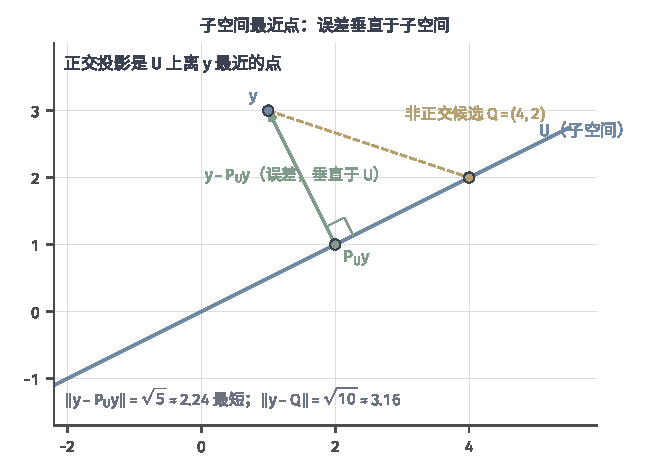
\includegraphics[width=112mm]{figures/00-shared/mathematical-preliminaries-upper/02-linear-spaces/matplotlib/ls-orthogonal-projection-nearest/ls-orthogonal-projection-nearest.pdf}
  \caption{直线子空间$U$（过原点、方向$(2,1)$）上离$\bm y=(1,3)^\top$最近的点是正交投影
  $\bm p=(2,1)^\top$，误差$\bm y-\bm p=(-1,2)^\top$与$U$垂直（直角小方块）；
  同一线上的另一候选$\bm q=(4,2)^\top$到$\bm y$的距离$\sqrt{10}$明显大于最短距离$\sqrt5$。
  这是解析式教学构造。}
  \label{fig:ls-orthogonal-projection-nearest}
\end{figure}

\paragraph{正规方程}

回到矩阵$\bm A$，取$U=\operatorname{range}(\bm A)$，设最近点是$\hat{\bm b}=\bm A\hat{\bm x}$。
列空间由$\bm A$的各列张成，残差$\bm r=\bm b-\bm A\hat{\bm x}$与列空间正交，就是与每一列$\bm a_j$正交，
即$\bm a_j^\top\bm r=0$，$j=1,\ldots,d$，合写为$\bm A^\top\bm r=\bm0$。代入$\bm r$得到\term{正规方程}（normal equations）
\begin{equation}
\begin{gathered}
\bm A^\top(\bm b-\bm A\hat{\bm x})=\bm0\\
\bm A^\top\bm A\hat{\bm x}=\bm A^\top\bm b.
\end{gathered}
\label{eq:linear-algebra-normal-equations}
\end{equation}
“正规”指法向，即残差与列空间正交，不是归一化。由定理~\ref{thm:ls-four-subspaces-orthogonality}，
这也就是说残差落在左零空间$\operatorname{null}(\bm A^\top)$中：最小二乘把$\bm b$分成可达的部分与完全不可达的部分。
下面用一个三个方程、两个未知量的例子计算正规方程。

\begin{example}[超定方程的最小二乘解]
\label{ex:ls-normal-equations-three-by-two}
取$\bm A=\left[\begin{smallmatrix}1&0\\0&1\\1&1\end{smallmatrix}\right]$、$\bm b=(2,3,2)^\top$。
列空间中的向量形如$(x_1,x_2,x_1+x_2)^\top$，第三坐标等于前两坐标之和；而$\bm b$的第三坐标$2\neq2+3$，
所以$\bm b$不在列空间中，方程$\bm A\bm x=\bm b$无解。计算
\[
\begin{gathered}
\bm A^\top\bm A=\begin{bmatrix}2&1\\1&2\end{bmatrix}\\
\bm A^\top\bm b=\begin{bmatrix}4\\5\end{bmatrix},
\end{gathered}
\]
解正规方程$2\hat x_1+\hat x_2=4$、$\hat x_1+2\hat x_2=5$，得$\hat{\bm x}=(1,2)^\top$。
最近点为$\bm A\hat{\bm x}=(1,2,3)^\top$，残差为$\bm r=\bm b-\bm A\hat{\bm x}=(1,1,-1)^\top$；
它与两列$(1,0,1)^\top$、$(0,1,1)^\top$的内积都是零，满足正交性判据。
\end{example}

图~\ref{fig:ls-least-squares-residual}画出这个例子。

\begin{figure}[htbp]
  \centering
  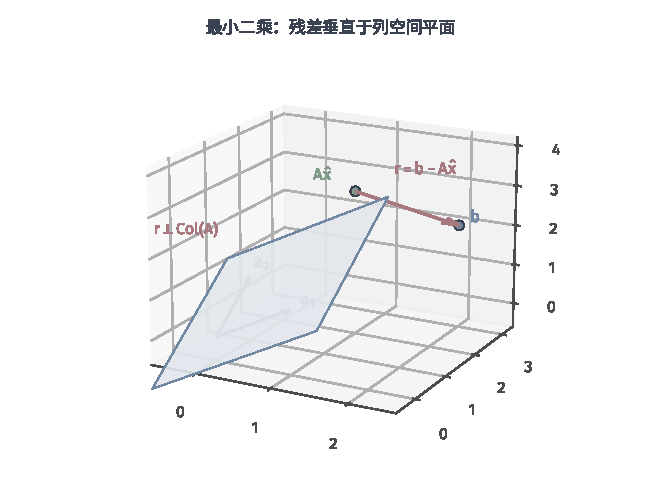
\includegraphics[width=112mm]{figures/00-shared/mathematical-preliminaries-upper/02-linear-spaces/matplotlib/ls-least-squares-residual/ls-least-squares-residual.pdf}
  \caption{列空间平面上的最近点。$\bm A=\left[\begin{smallmatrix}1&0\\0&1\\1&1\end{smallmatrix}\right]$，
  列$\bm a_1=(1,0,1)^\top$、$\bm a_2=(0,1,1)^\top$张成浅蓝平面；$\bm b=(2,3,2)^\top$，
  最近拟合值$\bm A\hat{\bm x}=(1,2,3)^\top$，残差$\bm r=(1,1,-1)^\top$满足
  $\bm r^\top\bm a_1=\bm r^\top\bm a_2=0$。透视教学构造。}
  \label{fig:ls-least-squares-residual}
\end{figure}

正规方程是由几何判据推出的；也可以直接验证，它的解确实使目标取全局最小。

设$\hat{\bm x}$满足正规方程，
$\bm r=\bm b-\bm A\hat{\bm x}$，对任意增量$\bm h$，$\bm A(\hat{\bm x}+\bm h)-\bm b=\bm A\bm h-\bm r$，展开平方长度得
\[
 \lVert\bm A(\hat{\bm x}+\bm h)-\bm b\rVert_2^2
 =\lVert\bm r\rVert_2^2-2(\bm A\bm h)^\top\bm r+\lVert\bm A\bm h\rVert_2^2
 =\lVert\bm r\rVert_2^2-2\bm h^\top(\bm A^\top\bm r)+\lVert\bm A\bm h\rVert_2^2 .
\]
正规方程使中间项为零，剩下的$\lVert\bm A\bm h\rVert_2^2\geq0$，所以任何移动都不会减小目标。
反之，若$\hat{\bm x}$是最小点，则拟合值$\bm A\hat{\bm x}$是列空间中离$\bm b$最近的点，由正交性判据，
残差与列空间正交，$\hat{\bm x}$满足正规方程。于是最小二乘问题与正规方程同解，
求最小点就是解这个$d$阶对称线性方程。

用一般子空间的基矩阵$\bm B$代替$\bm A$，并在一般内积下把$\bm B^\top\bm B$的元素换成内积，正规方程成为
\begin{equation}
\begin{gathered}
\bm G\bm c=\bigl(\langle\bm b_i,\bm y\rangle\bigr)_{i=1}^r\\
g_{i,j}=\langle\bm b_i,\bm b_j\rangle,
\end{gathered}
\label{eq:ls-gram-system}
\end{equation}
系数矩阵$\bm G$是基向量的Gram矩阵；逐行写就是$\sum_j\langle\bm b_i,\bm b_j\rangle c_j=\langle\bm b_i,\bm y\rangle$，
即残差$\bm y-\sum_jc_j\bm b_j$与每个基向量正交。这就把问题~\eqref{eq:ls-nearest-point-coefficients}化成了线性方程。

在示例~\ref{ex:ls-nonorthogonal-coefficients}中，$\bm G=\left[\begin{smallmatrix}2&1\\1&1\end{smallmatrix}\right]$，右端为$(1,0)^\top$，
解得$\bm c=(1,-1)^\top$，与直接观察一致。这里两个基向量张成整个平面，所以最近点就是$\bm y$本身；
Gram系统的作用是把内积$(1,0)^\top$纠正为真正的系数。

基向量标准正交时，Gram矩阵是单位矩阵，Gram系统不必求解：系数就是内积，最近点直接写出，
\[
 \bm p=\sum_j\langle\bm q_j,\bm y\rangle\bm q_j .
\]
这就是第~\ref{chap:normed-inner-product-spaces}章的正交分解公式~\eqref{eq:ls-orthonormal-projection}，每个系数只与自己的方向有关，互不干扰。
它是第~\ref{sec:ls-qr-method}节用QR分解解最小二乘的出发点。

\subsection{解的存在与唯一性}
\label{sec:ls-ls-existence}

最近点$\hat{\bm b}$作为列空间中的点总是存在且唯一，但正规方程的未知量是产生它的输入$\hat{\bm x}$。
本部分回答：这样的输入是否总存在，是否唯一，不唯一时全部解是什么样子，唯一时系数是否可靠。

\paragraph{存在性}

正规方程对任意$\bm b$都有解。几何上这很自然：$\hat{\bm b}$在列空间中，总有输入产生它，而这个输入满足正规方程。
也可以从方程本身验证。先看系数矩阵的零空间：若$\bm A^\top\bm A\bm x=\bm0$，则
$\lVert\bm A\bm x\rVert_2^2=\bm x^\top\bm A^\top\bm A\bm x=0$，即$\bm A\bm x=\bm0$；反向包含显然。故
\begin{equation}
 \ker(\bm A^\top\bm A)=\ker\bm A.
 \label{eq:ls-normal-kernel}
\end{equation}
由定理~\ref{thm:ls-four-subspaces-orthogonality}，对任意矩阵有$\operatorname{range}(\bm A^\top)=(\ker\bm A)^\perp$。把它用在对称矩阵$\bm A^\top\bm A$上，得
$\operatorname{range}(\bm A^\top\bm A)=\ker(\bm A^\top\bm A)^\perp=(\ker\bm A)^\perp=\operatorname{range}(\bm A^\top)$。
右端$\bm A^\top\bm b$显然在$\operatorname{range}(\bm A^\top)$中，所以方程总是相容。

\paragraph{全部解与唯一性}

拟合值唯一，不代表输入唯一。正规方程是相容的线性方程，按第~\ref{sec:ls-uniqueness-freedom}节的结论，它的全部解是一个解加上系数矩阵的零空间；
由~\eqref{eq:ls-normal-kernel}，全部解为
\begin{equation}
 \hat{\bm x}+\ker\bm A.
 \label{eq:ls-all-ordinary-solutions}
\end{equation}
这些解给出同一个拟合值，因为零空间方向不改变输出。于是解唯一当且仅当$\bm A$满列秩。
此时$\bm A^\top\bm A$正定（$\bm x\neq\bm0$时$\bm x^\top\bm A^\top\bm A\bm x=\lVert\bm A\bm x\rVert_2^2>0$），因而可逆，唯一解为
\begin{equation}
 \hat{\bm x}=(\bm A^\top\bm A)^{-1}\bm A^\top\bm b.
 \label{eq:linear-algebra-full-rank-least-squares}
\end{equation}
用子空间的基表示时同样如此：基向量线性无关，Gram矩阵$\bm G$正定，Gram系统~\eqref{eq:ls-gram-system}的解唯一。

这里有两层唯一性要分清。最近点作为$U$中的点总是唯一的；它的系数只在张成向量线性无关时唯一：
若$\bm B\bm c_1=\bm B\bm c_2$，则$\bm B(\bm c_1-\bm c_2)=\bm0$，线性无关迫使$\bm c_1=\bm c_2$。

秩亏时，例如$\bm A$有两列相同，正规方程相容但有无穷多解，第~\ref{sec:ls-select-among-solutions}节的讨论原样适用：
若要求欧氏范数最小，就去掉不改变输出的零空间分量，所得的解落在$(\ker\bm A)^\perp$中，
它也是相容方程$\bm A\bm x=\hat{\bm b}$的最小范数解。
在任意秩下把这一选择写成矩阵需要伪逆，见第~\ref{sec:ls-pseudoinverse}节。

无论解是否唯一，最小值都只由正交分解决定。$\hat{\bm b}\perp\bm r$，勾股恒等式给出
$\lVert\bm b\rVert_2^2=\lVert\hat{\bm b}\rVert_2^2+\lVert\bm r\rVert_2^2$：
观测的平方长度分成被列空间解释的部分与残差部分，最小平方残差
$\lVert\bm r\rVert_2^2=\lVert\bm b\rVert_2^2-\lVert\hat{\bm b}\rVert_2^2$对全部解相同。
示例~\ref{ex:ls-normal-equations-three-by-two}中，$\lVert\bm b\rVert_2^2=17$，$\lVert\hat{\bm b}\rVert_2^2=1+4+9=14$，$\lVert\bm r\rVert_2^2=3$。

\paragraph{唯一不等于稳定}

满列秩只保证系数唯一，不保证系数可靠。下面的例子中，设计矩阵的两列接近共线。

\begin{example}[近共线设计：唯一但不稳定的系数]
\label{ex:ls-nearly-collinear-design}
取互相正交的向量$\bm c_1=(1,1,1)^\top$与$\bm q=(0,1,-1)^\top$。
设计矩阵$\bm X_\varepsilon$的两列为$\bm c_1$与$\bm c_1+\varepsilon\bm q$，响应为$\bm y=\bm c_1+\delta\bm q$。
利用$\bm c_1^\top\bm q=0$、$\lVert\bm c_1\rVert_2^2=3$、$\lVert\bm q\rVert_2^2=2$，正规方程为
\[
 \begin{bmatrix}3&3\\3&3+2\varepsilon^2\end{bmatrix}\hat{\bm w}
 =\begin{bmatrix}3\\3+2\varepsilon\delta\end{bmatrix},
\]
系数矩阵的行列式为$6\varepsilon^2$。$\varepsilon\neq0$时满列秩，解为
\begin{equation}
\begin{gathered}
\hat{\bm w}_\varepsilon
 =\begin{bmatrix}1-\delta/\varepsilon\\\delta/\varepsilon\end{bmatrix}\\
\bm X_\varepsilon\hat{\bm w}_\varepsilon=\bm y,
\end{gathered}
\label{eq:linear-algebra-nearly-collinear-least-squares}
\end{equation}
后一式可直接验证：$(1-\delta/\varepsilon)\bm c_1+(\delta/\varepsilon)(\bm c_1+\varepsilon\bm q)=\bm c_1+\delta\bm q$。
取$\varepsilon=0.01$、$\delta=0.1$，系数为$(-9,10)^\top$，残差却为零。

$\varepsilon=0$时两列重合为$\bm c_1$。此时$\bm y=\bm c_1+\delta\bm q$本身就是正交分解，最近输出为$\bm c_1$，
残差为$\delta\bm q$，平方残差为$2\delta^2$；满足$w_1+w_2=1$的系数都是解。
\end{example}

所以$\delta\neq0$时，随着$\varepsilon\to0$，精确拟合所需的系数趋于无穷，而极限矩阵已经不能精确拟合。
拟合值可以相当稳定，表示它的两个系数却可能很大，而且对$\varepsilon$、$\delta$极为敏感。
这是近共线几何本身的性质，不是计算机舍入造成的；它的定量刻画见第~\ref{sec:ls-ordinary-ls-sensitivity}节。

\subsection{正规方程法}
\label{sec:ls-normal-equations-method}

本小节的输入仍是$\bm A\in\mathbb R^{m\times d}$与$\bm b\in\mathbb R^m$，这里假设$m\geq d$且$\bm A$满列秩。原方程可能不相容，因此输出改为唯一的最小二乘解$\hat{\bm x}$。

上一小节已经把最优性写成$\bm A^\top(\bm b-\bm A\hat{\bm x})=0$；正规方程法直接把这个条件当作待求解的$d$阶正定方程。

最直接的算法是解正规方程。$\bm A$满列秩时$\bm A^\top\bm A$对称正定，可以用Cholesky分解：
先形成$\bm A^\top\bm A$与$\bm A^\top\bm b$，分解$\bm A^\top\bm A=\bm L\bm L^\top$，再依次前代解$\bm L\bm z=\bm A^\top\bm b$、
回代解$\bm L^\top\hat{\bm x}=\bm z$。加权问题对$\bm A^\top\bm M\bm A$作同样的分解。
稠密情形下，形成$\bm A^\top\bm A$约需$md^2$次乘法，分解约需$d^3/3$次运算，多个右端复用同一分解。
$m$远大于$d$且矩阵条件良好时，形成正规矩阵再作Cholesky分解，通常比稠密QR所需运算更少。

例如仍用$\bm A=\left[\begin{smallmatrix}1&0\\0&1\\1&1\end{smallmatrix}\right]$和$\bm b=(2,3,2)^\top$。先算出
\[
 \bm G=\bm A^\top\bm A=\begin{bmatrix}2&1\\1&2\end{bmatrix},\qquad
 \bm c=\bm A^\top\bm b=\begin{bmatrix}4\\5\end{bmatrix}.
\]
Cholesky因子为$\bm L=\left[\begin{smallmatrix}\sqrt2&0\\1/\sqrt2&\sqrt{3/2}\end{smallmatrix}\right]$。前代$\bm L\bm z=\bm c$得到$\bm z=(2\sqrt2,\sqrt6)^\top$，回代$\bm L^\top\hat{\bm x}=\bm z$得到$\hat{\bm x}=(1,2)^\top$。原残差为$(1,1,-1)^\top$，虽非零，却满足$\bm A^\top\bm r=0$，这才是最小二乘计算要核验的条件。

形成$\bm A^\top\bm A$会损失精度。由第~\ref{sec:ls-svd}节的奇异值分解，$\bm A^\top\bm A$的特征值是$\bm A$的奇异值的平方：
$\bm A$中被压缩得很厉害的方向，在$\bm A^\top\bm A$中被压缩两次，就像一个小数取平方后更小；
浮点计算中，这种方向可能与零无法区分。所以正规方程法只在各列明显线性无关、
$\bm A^\top\bm A$的正定性有充足余量时可靠。秩亏时唯一性本身就不成立；近秩亏时，如示例~\ref{ex:ls-nearly-collinear-design}，
系数本来就不稳定，Cholesky分解成功也不说明结果可用。这种平方造成的精度损失在第~\ref{sec:ls-numerical-sensitivity}节用条件数定量估计。

\subsection{QR分解}
\label{sec:ls-qr-method}
\label{sec:linear-algebra-direct-residual}

另一条路线不形成$\bm A^\top\bm A$，而是先给列空间换一组标准正交基。
第~\ref{chap:normed-inner-product-spaces}章的Gram--Schmidt正交化正是做这件事，它把满列秩矩阵写成经济型QR分解
$\bm A=\bm Q\bm R$（式~\eqref{eq:ls-qr-factorization}），$\bm Q$的列是列空间的标准正交基，$\bm R$是对角元为正的上三角矩阵。
QR适合最小二乘的根本原因是：正交矩阵保持欧氏长度，用它变换残差，只改坐标，不改长度，最小点也就不变。

设$\bm A$满列秩，把$\bm Q$的列扩充成$\mathbb R^m$的标准正交基，得到完全QR分解
$\bm A=[\bm Q_1\;\bm Q_2]\left[\begin{smallmatrix}\bm R\\\bm0\end{smallmatrix}\right]=\bm Q_1\bm R$，
其中$[\bm Q_1\;\bm Q_2]$是$m$阶正交矩阵，$\bm Q_1$有$d$列，就是经济型分解中的$\bm Q$；$\bm Q_2$的列张成列空间的正交补。
记$\bm c_1=\bm Q_1^\top\bm b$、$\bm c_2=\bm Q_2^\top\bm b$。用$[\bm Q_1\;\bm Q_2]^\top$变换残差，
\[
 \lVert\bm A\bm x-\bm b\rVert_2^2
 =\left\lVert\begin{bmatrix}\bm R\bm x-\bm c_1\\-\bm c_2\end{bmatrix}\right\rVert_2^2
 =\lVert\bm R\bm x-\bm c_1\rVert_2^2+\lVert\bm c_2\rVert_2^2 .
\]
第二项与$\bm x$无关，是无法消除的残差；第一项可以通过解上三角方程$\bm R\hat{\bm x}=\bm c_1$降为零。
满列秩时$\bm R$的对角元非零，回代即得唯一解，最小平方残差就是$\lVert\bm c_2\rVert_2^2=\lVert\bm b\rVert_2^2-\lVert\bm c_1\rVert_2^2$，
所以$\bm Q_2$不必形成。整个过程不出现$\bm A^\top\bm A$，避免了正规方程法的平方尺度损失，
代价是分解的运算量高于Cholesky。

下面用QR分解重算示例~\ref{ex:ls-normal-equations-three-by-two}。

\begin{example}[用QR分解求解最小二乘]
\label{ex:ls-qr-three-by-two}
仍取$\bm A=\left[\begin{smallmatrix}1&0\\0&1\\1&1\end{smallmatrix}\right]$、$\bm b=(2,3,2)^\top$。
Gram--Schmidt先给出$\bm q_1=(1,0,1)^\top/\sqrt2$。$\bm a_2$在$\bm q_1$上的分量为$r_{1,2}=\bm q_1^\top\bm a_2=1/\sqrt2$，扣除后
\[
 \begin{gathered}
\bm v_2=(0,1,1)^\top-\tfrac12(1,0,1)^\top=(-\tfrac12,1,\tfrac12)^\top\\
r_{2,2}=\lVert\bm v_2\rVert_2=\sqrt{3/2},
 \end{gathered}
\]
再令$\bm q_2=\bm v_2/r_{2,2}$。于是
\[
\begin{gathered}
\bm R=\begin{bmatrix}\sqrt2&1/\sqrt2\\0&\sqrt{3/2}\end{bmatrix}\\
\bm c_1=\begin{bmatrix}\bm q_1^\top\bm b\\\bm q_2^\top\bm b\end{bmatrix}=\begin{bmatrix}2\sqrt2\\\sqrt6\end{bmatrix}.
\end{gathered}
\]
回代解$\bm R\hat{\bm x}=\bm c_1$，得$\hat x_2=\sqrt6/\sqrt{3/2}=2$、$\hat x_1=(2\sqrt2-2/\sqrt2)/\sqrt2=1$，
与正规方程的结果相同。最小平方残差为$\lVert\bm b\rVert_2^2-\lVert\bm c_1\rVert_2^2=17-(8+6)=3$，也与前面一致。
\end{example}

同一分解还给出最近点。最近点为$\hat{\bm b}=\bm A\hat{\bm x}=\bm Q_1\bm R\hat{\bm x}=\bm Q_1\bm c_1=\bm Q_1\bm Q_1^\top\bm b$，
$\bm c_1$的分量就是$\bm b$在各正交方向上的坐标，不必另解Gram系统。

它也判定相容性：$\bm c_2=\bm0$当且仅当$\bm b$在列空间中，
此时回代得到的就是原方程的精确解；$\bm c_2\neq\bm0$时原方程不相容，$\lVert\bm c_2\rVert_2$就是$\bm b$到列空间的距离。
例如$\bm A=\left[\begin{smallmatrix}1&1\\1&0\\0&1\end{smallmatrix}\right]$、$\bm b=(2,1,1)^\top=\bm A(1,1)^\top$时$\bm c_2=\bm0$，
回代得到精确解$\hat{\bm x}=(1,1)^\top$。这就是第~\ref{sec:ls-direct-methods}节所说的：
超定而满列秩的方程，相容性的判断与唯一解的计算可以由同一个QR分解一次完成。

$\bm A$秩亏时，Gram--Schmidt在某一列得不到新方向，$\bm R$不再可逆，上面的回代不能直接进行；
这时最小二乘解不唯一，最小范数解由第~\ref{sec:ls-pseudoinverse}节的伪逆给出。
有限精度下怎样借带列主元的QR判断秩，见第~\ref{sec:ls-orthogonalization-qr}节。

\paragraph{列空间投影与正规方程}

不做正交化，也可以从正规方程写出投影矩阵。$\bm A$满列秩时，最近点为
$\hat{\bm b}=\bm A\hat{\bm x}=\bm A(\bm A^\top\bm A)^{-1}\bm A^\top\bm b$，故
\begin{equation}
 \bm P_{\operatorname{range}(\bm A)}=\bm A(\bm A^\top\bm A)^{-1}\bm A^\top.
 \label{eq:ls-column-space-projector}
\end{equation}
直接相乘可验它对称且幂等。代入$\bm A=\bm Q\bm R$，得$\bm Q\bm R(\bm R^\top\bm R)^{-1}\bm R^\top\bm Q^\top=\bm Q\bm Q^\top$，
与式~\eqref{eq:linear-algebra-orthogonal-projector}一致，说明投影只取决于列空间，与所用的基无关。

回归中这个矩阵常称帽子矩阵，它把观测$\bm y$映成拟合值$\hat{\bm y}$；$\bm I-\bm P$则把观测映成残差，
它是到$\operatorname{range}(\bm A)^\perp=\operatorname{null}(\bm A^\top)$的正交投影。
加权内积下，同样的推导给出$\bm A(\bm A^\top\bm M\bm A)^{-1}\bm A^\top\bm M$；它幂等但一般不对称，
在普通内积下是斜投影，在$\bm M$内积下才是正交投影。

两个正交投影相乘一般不可交换，$\bm P_U\bm P_V\neq\bm P_V\bm P_U$，乘积也未必还是投影。
两者可交换时，乘积既幂等又对称，因而是到其像的正交投影。它的像含于$U$（左因子是$\bm P_U$），
也含于$V$（交换次序后左因子是$\bm P_V$），而$U\cap V$中的向量被它保持不变，所以它是到$U\cap V$的正交投影。


\subsection{修正Gram--Schmidt正交化}

上面已经说明如何用QR分解把最小二乘化为三角方程，现在还需说明分解本身怎样计算。
第~\ref{chap:normed-inner-product-spaces}章用Gram--Schmidt正交化构造它，那里假定精确算术：
式~\eqref{eq:ls-gram-schmidt}一次性减去$\bm a_j$在全部旧方向上的分量，每个系数都用原始的$\bm a_j$计算。

\term{修正Gram--Schmidt}（modified Gram--Schmidt）改为逐个扣除：先令$\bm u\leftarrow\bm a_j$，对$i=1,\ldots,j-1$依次计算$r_{i,j}=\langle\bm u,\bm q_i\rangle$并更新$\bm u\leftarrow\bm u-r_{i,j}\bm q_i$，最后归一化。

具体说，第$j$列处理结束后，令$r_{j,j}=\|\bm u\|_2$、$\bm q_j=\bm u/r_{j,j}$；若该范数为零，当前列不能提供新方向，应转入秩亏处理。对$j=1,\ldots,d$重复，输出$\bm Q=[\bm q_1\;\cdots\;\bm q_d]$与$\bm R=(r_{i,j})$。

随后计算$c_j=\bm q_j^\top\bm b$并回代$\bm R\hat{\bm x}=\bm c$，才完成输入$(\bm A,\bm b)$到最小二乘解的过程。前面的三行两列算例中，第二列只有一个旧方向可扣除，按这一流程同样得到$\hat{\bm x}=(1,2)^\top$。

精确算术中两种做法给出同样的结果：扣除第$i$个方向时，此前已减去的都是$\bm q_1,\ldots,\bm q_{i-1}$的倍数，它们与$\bm q_i$正交，所以$\langle\bm u,\bm q_i\rangle=\langle\bm a_j,\bm q_i\rangle$。

有限精度下，修正的做法每次都从已经扣除过的最新残差出发，算出的$\bm q_j$之间正交性的损失通常更小；
它的损失大致与$\kappa_2(\bm A)$乘单位舍入$u$同量级，原始做法则可能严重得多\scite{math-golub2013matrix}。
列之间越接近线性相关，扣除后剩下的$\bm u_j$越短，舍入误差在其中所占的比例越大，两种做法的差别也越明显。

同样的原因使列相关时的处理不能照搬精确算术：有限精度下$\bm u_j$很少恰好为零，判断“没有新方向”时要把$\lVert\bm u_j\rVert$与一个容限比较，
这正是第~\ref{sec:ls-ordinary-ls-sensitivity}节的数值秩问题。修正Gram--Schmidt的正交性损失仍随条件数增长；
需要$\bm Q$在工作精度下正交时，改用后面的Householder反射。

\subsection{Householder反射}
\label{sec:ls-orthogonalization-qr}

修正Gram--Schmidt仍从列出发构造$\bm Q$，列越接近线性相关，正交性损失越大，而这恰是最需要QR的情形。
稠密计算中更常用的做法反过来：用一串正交矩阵从左边作用于$\bm A$，逐列把主对角线以下的元素消成零，最后剩下上三角的$\bm R$。
正交矩阵保持长度，这样的消元不会放大误差，各步正交矩阵的乘积自然是正交的。
完成这一步的基本工具是\term{Householder反射}，它一次消去一列中主对角线以下的全部元素。

对非零向量$\bm a$，要找一个正交矩阵把它变成$\bm e_1$的倍数。由于正交变换保持长度，目标只能是$\pm\lVert\bm a\rVert_2\bm e_1$。
取$s=1$（若$a_1\geq0$）或$s=-1$（若$a_1<0$），令
\begin{equation}
\begin{gathered}
\bm v=\bm a+s\lVert\bm a\rVert_2\bm e_1\\
\bm H=\bm I-2\frac{\bm v\bm v^\top}{\bm v^\top\bm v}.
\end{gathered}
\label{eq:ls-householder}
\end{equation}
$\bm H$把$\bm v$方向的分量变号，与$\bm v$正交的分量保持不变，即关于以$\bm v$为法向的超平面作镜面反射；
它对称，且$\bm H^\top\bm H=\bm H^2=\bm I$，反射两次回到原处。

下面验证它把$\bm a$送到$\bm e_1$方向。记$\alpha=\lVert\bm a\rVert_2$，则
$\bm v^\top\bm a=\alpha^2+s\alpha a_1$，$\bm v^\top\bm v=\alpha^2+2s\alpha a_1+\alpha^2=2\bm v^\top\bm a$，于是
\[
 \bm H\bm a=\bm a-2\frac{\bm v^\top\bm a}{\bm v^\top\bm v}\bm v=\bm a-\bm v=-s\alpha\bm e_1 .
\]
符号$s$取与$a_1$相同，是为了让$\bm v$的首元素$a_1+s\alpha$是两个同号数相加，避免两个相近的数相减而丢失有效数字。
应用$\bm H$时只需保存$\bm v$，计算$\bm H\bm x=\bm x-2\bm v(\bm v^\top\bm x)/(\bm v^\top\bm v)$，不必形成整个矩阵。

\begin{example}[二维向量的Householder反射]
\label{ex:ls-householder-two-dim}
取$\bm a=(3,4)^\top$。$a_1>0$，取$s=1$；$\alpha=5$，$\bm v=\bm a+5\bm e_1=(8,4)^\top$，$\bm v^\top\bm v=80$。于是
\[
 \bm H=\bm I-\frac{2}{80}\bm v\bm v^\top
 =\bm I-\frac1{40}\begin{bmatrix}64&32\\32&16\end{bmatrix}
 =\begin{bmatrix}-3/5&-4/5\\-4/5&3/5\end{bmatrix},
\]
$\bm H\bm a=(-5,0)^\top$，与$-s\alpha\bm e_1=-5\bm e_1$一致。
\end{example}

对矩阵做QR时，第$k$步对第$k$列从第$k$个元素往下的部分构造反射，
只作用于尚未处理的右下子块。$d$步之后，$\bm H_d\cdots\bm H_1\bm A=\left[\begin{smallmatrix}\bm R\\\bm0\end{smallmatrix}\right]$，
各反射的乘积的转置就是完全QR分解中的$[\bm Q_1\;\bm Q_2]$；
$\bm R$的对角元可能为负，把相应的行与$\bm Q_1$的列同时变号即可化为对角元为正的形式。

把这一过程用于求解时，令工作矩阵$\bm F=\bm A$、工作右端$\bm c=\bm b$。第$k$步用$\bm F_{k:m,k}$构造反射，把它同时作用于$\bm F_{k:m,k:d}$与$\bm c_{k:m}$；前面已经消出的零不再改变。全部列处理完后，$\bm F$的前$d$行是$\bm R$，$\bm c$的前$d$项是$\bm c_1$，回代得到$\hat{\bm x}$，其余项组成不可消除的残差坐标$\bm c_2$。

若为统一符号而翻转$\bm R$某行，也须同步翻转$\bm c_1$的对应项。

例如取$\bm A=\left[\begin{smallmatrix}3&1\\4&2\end{smallmatrix}\right]$、$\bm b=(4,6)^\top$。用上例的反射同时变换二者，得到
\[
 \bm H\bm A=\begin{bmatrix}-5&-11/5\\0&2/5\end{bmatrix},\qquad
 \bm H\bm b=\begin{bmatrix}-36/5\\2/5\end{bmatrix}.
\]
由第二行得$x_2=1$，再由第一行得$x_1=1$。反射后的矩阵已经是上三角形，因而本例无需继续消元；代回可验$\bm A\bm x=\bm b$。

稠密$m\times d$矩阵的Householder QR约需$2md^2-2d^3/3$次浮点运算。$\bm Q$不必显式形成，
保存各步的反射向量即可；求解最小二乘时，把同样的反射依次作用于$\bm b$就得到$\bm c_1$与$\bm c_2$，
多个右端复用全部反射与$\bm R$。岭回归对堆叠矩阵~\eqref{eq:ls-augmented-system}作同样的分解即可，
不必形成$\bm A^\top\bm A+\lambda\bm L^\top\bm L$。

秩亏或接近秩亏时，要先把列重新排序。带列主元的QR在每一步选剩余部分中最长的一列先处理，
使接近零的对角元集中在$\bm R$的尾部，从而暴露数值秩，阈值按数据误差的尺度选取，这比计算奇异值分解便宜。
若精确秩为$r$，只用前$r$个主元列回代、其余未知量取零，得到的基本解使原目标达到最小，
但一般不是最小范数解，正如第~\ref{sec:ls-select-among-solutions}节中自由变量取零得到的特解一般不是最小范数解。若$r$由数值阈值确定，被忽略的方向未必精确为零，此时得到的是截断近似，不能保证它是原问题的精确最小二乘解。

\subsection{Givens旋转}

Householder一次处理整段列向量；当只需消去少数元素，或者新观测只增加了一行时，重新反射整个子块可能不划算。Givens方法只混合两行，同步更新这两行的系数与右端，仍以得到三角方程并回代为目标。输入输出与Householder求解相同，差别在于每一步消元的范围。

\term{Givens旋转}一次只消去一个元素。它在第$i$、$j$两个坐标构成的平面内作旋转，其余坐标不变；
在这两个坐标上的作用是
\begin{equation}
\begin{gathered}
\begin{bmatrix}a_i\\a_j\end{bmatrix}\mapsto
 \begin{bmatrix}c&s\\-s&c\end{bmatrix}
 \begin{bmatrix}a_i\\a_j\end{bmatrix}\\
c^2+s^2=1.
\end{gathered}
\label{eq:ls-givens}
\end{equation}
这里的$c$、$s$是旋转角的余弦与正弦，与Householder反射中的符号$s$无关。
完整的矩阵$\bm G(i,j)$是在单位矩阵的$(i,i),(i,j),(j,i),(j,j)$四个位置放上$c,s,-s,c$。
为了消去$a_j$，取$r=\sqrt{a_i^2+a_j^2}$，$c=a_i/r$、$s=a_j/r$，则新分量为
$(ca_i+sa_j,\,-sa_i+ca_j)=(r,0)$。$r=0$时两个分量本已为零，无需旋转。

\begin{example}[二维向量的Givens旋转]
\label{ex:ls-givens-two-dim}
取$(a_i,a_j)=(3,4)$。$r=\sqrt{9+16}=5$，$c=3/5$、$s=4/5$，旋转后
\[
 \begin{gathered}
ca_i+sa_j=\frac95+\frac{16}5=5\\
-sa_i+ca_j=-\frac{12}5+\frac{12}5=0 ,
 \end{gathered}
\]
第二个分量被消去，长度$5$全部转到第一个分量上。
\end{example}

对一般$m\times d$的输入，先令$\bm F=\bm A$、$\bm c=\bm b$。按列$k=1,\ldots,d$处理，每列从底部$i=m$向上到$k+1$，对当前的$f_{i-1,k},f_{i,k}$构造旋转，混合第$i-1,i$行的第$k$至$d$列，并同步混合$c_{i-1},c_i$。这样逐个把对角线以下的元素消为零，而且不会破坏前面列中的零。最后取前$d$行得到$\bm R$，回代$\bm R\hat{\bm x}=\bm c_{1:d}$。

在上一小节同一个二阶方程中，旋转矩阵取$\bm G=\left[\begin{smallmatrix}3/5&4/5\\-4/5&3/5\end{smallmatrix}\right]$，得到$\bm G\bm A=\left[\begin{smallmatrix}5&11/5\\0&2/5\end{smallmatrix}\right]$与$\bm G\bm b=(36/5,2/5)^\top$。回代仍得$(1,1)^\top$。两种正交变换的中间符号不同，最终求解的是同一个原方程。

Givens每次只改动两行，适合稀疏或带状矩阵，也适合在最小二乘中新增一条观测时逐步更新已有的QR；
对稠密矩阵，它消去同样多的元素需要更多运算，不如Householder。
图~\ref{fig:ls-givens-householder-elimination}把两种变换并置。图中的反射取另一种符号，
把向量映到$(r,0)^\top$而不是$(-r,0)^\top$，精确算术中两种选择都可以。

\begin{figure*}[htbp]
  \centering
  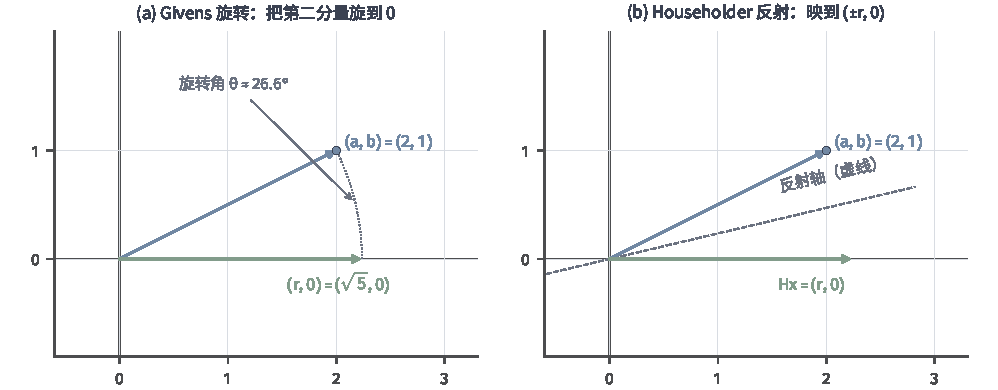
\includegraphics[width=168.998mm]{figures/00-shared/mathematical-preliminaries-upper/02-linear-spaces/matplotlib/ls-givens-householder-elimination/ls-givens-householder-elimination.pdf}
  \caption{两种初等正交消元。左：Givens旋转把$(a,b)=(2,1)^\top$沿圆弧旋到
  $(r,0)^\top$，$r=\sqrt5$，旋转角$\theta=\arctan(1/2)$；右：Householder反射沿角平分线
  把同一向量映到$(r,0)^\top$。两者都是正交变换，保持长度，区别在旋转（行列式$+1$）与
  反射（对称正交）。解析式教学构造。}
  \label{fig:ls-givens-householder-elimination}
\end{figure*}

至此，正规方程与QR都给出了完整的直接求解过程：前者形成正定系统，后者把系数和右端一起作正交变换，再解三角方程。当矩阵很大、无法方便地保存这些因子时，下一组方法用矩阵向量乘法逐步构造小问题。
% LSMR recursion checked against Fong and Saunders, SIAM J. Sci. Comput. 33 (2011), Algorithm LSMR.
% Extended Kaczmarz uses the synchronous old-z update of Zouzias and Freris, arXiv:1205.5770, Algorithm 3.
\subsection{Golub--Kahan双对角化}
\label{sec:ls-bidiagonal-iteration}

前面的QR方法适合能够保存分解结果的问题。若$\bm A\in\mathbb R^{m\times d}$很大，或者只能够计算$\bm A\bm v$与$\bm A^\top\bm u$，可以逐步构造低维问题，每一步只使用这两种乘法。下面从零初值说明；非零初值可以先以$\bm b-\bm A\bm x_0$为右端项求修正，但还要单独检查所得解的零空间分量。

以下统一输入$\bm A,\bm b$、两种残差的容差与最大步数，初值固定为$\bm x_0=0$。LSQR与LSMR的最终输出都是$d$维近似解，区别是每个子空间中优化哪一种残差。双对角化只是二者共享的准备过程：它输出基向量及双对角系数，还没有给出近似解。

为什么要交替使用$\bm A$与$\bm A^\top$？$\bm A$把$d$维未知量送入$m$维观测空间，而最优性条件$\bm A^\top\bm r=0$又把观测残差送回未知量空间。分别在两个空间中保持正交基，就能用很少的系数记录这两个作用，并把大问题的残差精确地表示成小问题的残差。

若$\bm b=0$，零向量已是最小范数解。否则令$\beta_1=\lVert\bm b\rVert_2$、$\bm u_1=\bm b/\beta_1$，再计算$\alpha_1=\lVert\bm A^\top\bm u_1\rVert_2$。若$\alpha_1=0$，零向量已满足正规方程。

当$\alpha_1>0$时令$\bm v_1=\bm A^\top\bm u_1/\alpha_1$。Golub--Kahan双对角化按下式交替生成两个空间中的向量：
\begin{align*}
 \bm p&=\bm A\bm v_k-\alpha_k\bm u_k,\\
 \beta_{k+1}&=\lVert\bm p\rVert_2,\\
 \bm u_{k+1}&=\bm p/\beta_{k+1},\\
 \bm q&=\bm A^\top\bm u_{k+1}-\beta_{k+1}\bm v_k,\\
 \alpha_{k+1}&=\lVert\bm q\rVert_2,\\
 \bm v_{k+1}&=\bm q/\alpha_{k+1}.
\end{align*}

待归一化向量为零时，不能执行对应除法。

若$\beta_{k+1}=0$，当前$\bm B_k$的最后一个下对角元已知为零；此时可令后续旋转所需的$\alpha_{k+1}=0$作为终止时的约定，不定义$\bm u_{k+1}$或$\bm v_{k+1}$。若$\beta_{k+1}>0$但$\alpha_{k+1}=0$，则已知$\bm B_k$和该零值，也不定义$\bm v_{k+1}$。

两种情形都先用已生成的系数完成当前小问题及$\bm x_k$的更新，再检查原残差和正规残差，不构造后续不存在的基向量。

减去旧方向的分量使所得向量在精确算术中与已有基正交。

当$\beta_{k+1}>0$时，把已生成的$\bm u_i$和$\bm v_i$分别排成列，得到$\bm A\bm V_k=\bm U_{k+1}\bm B_k$，其中$\bm B_k$的主对角为$\alpha_1,\ldots,\alpha_k$，下对角为$\beta_2,\ldots,\beta_{k+1}$。若$\beta_{k+1}=0$，则去掉$\bm B_k$的全零末行，记剩余方阵为$\widehat{\bm B}_k$，此时使用$\bm A\bm V_k=\bm U_k\widehat{\bm B}_k$，无需构造$\bm u_{k+1}$。

\subsection{LSQR算法}

有了双对角化输出，下一步要决定原变量怎样取值。LSQR把候选解限制在$\operatorname{span}\{\bm v_1,\ldots,\bm v_k\}$中，并在其中最小化原残差。也就是说，输入数据未变，只把每轮需要选择的未知量从$d$个原坐标换成$k$个子空间坐标。

选择$\bm x_k=\bm V_k\bm y$，并利用$\bm b=\beta_1\bm u_1$与已生成的$\bm U$的正交性，原残差范数化为$\lVert\beta_1\bm e_1-\bm B_k\bm y\rVert_2$。末行因$\beta_{k+1}=0$而删去时，改用$\widehat{\bm B}_k$及$k$维的$\bm e_1$，结果相同。LSQR在每一步求解这个小型最小二乘问题；因此精确算术下，随着候选空间扩大，原残差范数不增。实现可以用Givens旋转逐步更新小问题，不必每轮重新分解，也不必形成$\bm A^\top\bm A$。避免形成正规矩阵能减少填充及其形成误差，却不能消除原问题的小奇异值。

具体实现时，可将新一行双对角元素用一次平面旋转消去，并同时更新解。初始化$\bm x_0=\bm0$、$\bm w_1=\bm v_1$、$\bar\rho_1=\alpha_1$、$\bar\phi_1=\beta_1$。第$k$轮先做上述双对角化，再依次计算
\begin{align*}
 \rho_k&=\sqrt{\bar\rho_k^2+\beta_{k+1}^2},\\
 c_k&=\bar\rho_k/\rho_k,\\
 s_k&=\beta_{k+1}/\rho_k,\\
 \theta_{k+1}&=s_k\alpha_{k+1},\\
 \bar\rho_{k+1}&=-c_k\alpha_{k+1},\\
 \phi_k&=c_k\bar\phi_k,\quad \bar\phi_{k+1}=s_k\bar\phi_k,
\end{align*}
并更新$\bm x_k=\bm x_{k-1}+(\phi_k/\rho_k)\bm w_k$与$\bm w_{k+1}=\bm v_{k+1}-(\theta_{k+1}/\rho_k)\bm w_k$。这些标量记录逐次旋转，小问题的解通过方向$\bm w_k$累加到原变量中。

这个累加式可以从回代读出，而无需把它当作独立公式记忆。旋转把双对角小矩阵化为上双对角矩阵，当前对角元是$\rho_k$，与下一列的耦合是$\theta_{k+1}$。把三角求解与$\bm V_k\bm y$合在一起，已消去的耦合由$\bm w_{k+1}=\bm v_{k+1}-(\theta_{k+1}/\rho_k)\bm w_k$记录；当前右端分量$\phi_k$除以$\rho_k$后，沿$\bm w_k$加回原解。因而无需每轮保存全部基再重新回代。

若双对角化在本轮产生零量，将所需的零系数代入当前旋转与$\bm x_k$的更新，再检查残差；此时不需要计算下一方向$\bm w_{k+1}$。若$\rho_k=0$，则不能执行相应除法，应直接处理已构造的小问题并检查所得解。

由于零初值下$\bm x_k$位于$\operatorname{range}(\bm A^\top)$，若迭代达到$\bm A^\top(\bm b-\bm A\bm x_k)=0$，它既是最小二乘解，又与$\operatorname{null}(\bm A)$正交，因而是最小范数解。有限精度下向量可能失去正交性，必要时可重正交化，但这需要额外存储与内积。每轮主要成本是一遍$\bm A$与一遍$\bm A^\top$的乘法；实际停止时既检查原残差，也检查正规残差，避免把不相容问题固有的非零残差误判为失败。

\subsection{LSMR算法}
\label{sec:ls-lsmr}

不相容的最小二乘问题中，原残差一般不能降到零；达到最小二乘解的条件是$\bm A^\top\bm r=\bm0$。LSMR与LSQR使用同一组双对角化向量，但在候选空间中选择使正规残差$\lVert\bm A^\top(\bm b-\bm A\bm x_k)\rVert_2$最小的近似。

当$\beta_{k+1}>0$且$\alpha_{k+1}>0$时，由双对角化关系，$\bm A^\top\bm U_{k+1}=\bm V_k\bm B_k^\top+\alpha_{k+1}\bm v_{k+1}\bm e_{k+1}^\top$。令$\bm x_k=\bm V_k\bm y$，得到
\[
 \bm A^\top(\bm b-\bm A\bm x_k)
 =\bm V_{k+1}\left(\alpha_1\beta_1\bm e_1-
 \begin{bmatrix}\bm B_k^\top\bm B_k\\
 \alpha_{k+1}\beta_{k+1}\bm e_k^\top\end{bmatrix}\bm y\right).
\]

所以可通过一个$(k+1)\times k$的小最小二乘问题选择$\bm y$。若$\alpha_{k+1}=0$而$\beta_{k+1}>0$，省去含$\bm v_{k+1}$的零项，使用已有的$\bm V_k$及小问题的前$k$行。若$\beta_{k+1}=0$，则用$\bm U_k$、$\bm V_k$和$\widehat{\bm B}_k$，正规残差为$\bm V_k(\alpha_1\beta_1\bm e_1-\widehat{\bm B}_k^\top\widehat{\bm B}_k\bm y)$；两种情形都不引入缺失的基向量。

这个矩阵用于解释方法；实际短递推利用双对角化系数和两组旋转，不形成原矩阵的$\bm A^\top\bm A$。候选空间逐步扩大，故精确算术中正规残差范数不增；这不意味着解误差也逐步下降。

具体计算可按下列顺序。

第一组旋转与LSQR一样，先把双对角作用化为三角作用；LSMR还要最小化经过$\bm A^\top$作用的残差，因此再用第二组旋转消去这一作用带来的耦合。下面的带横线标量保存旋转后的系数，$\bm h_k$与$\bar{\bm h}_k$保存将小问题的坐标恢复到原变量时所需的方向。每轮依次完成双对角化、两组旋转和解的更新，不能把某一组旋转单独当作解。

使用上一小节的$\alpha_1,\beta_1,\bm v_1$初始化
\[
 \begin{gathered}
\bar\alpha_1=\alpha_1\\
\bar\zeta_1=\alpha_1\beta_1\\
\rho_0=\bar\rho_0=\bar c_0=1\\
\bar s_0=0\\
\bm h_1=\bm v_1\\
\bar{\bm h}_0=\bm0\\
\bm x_0=\bm0.
 \end{gathered}
\]

每轮先继续双对角化，得到$\beta_{k+1}$、$\alpha_{k+1}$和$\bm v_{k+1}$。第一组旋转消去新出现的下对角元：
\[
 \begin{gathered}
\rho_k=\sqrt{\bar\alpha_k^2+\beta_{k+1}^2}\\
c_k=\frac{\bar\alpha_k}{\rho_k}\\
s_k=\frac{\beta_{k+1}}{\rho_k}\\
\theta_{k+1}=s_k\alpha_{k+1}\\
\bar\alpha_{k+1}=c_k\alpha_{k+1}.
 \end{gathered}
\]

第二组旋转处理正规残差小问题中的耦合。它使用上一轮保存的四个量：$\bar c_{k-1}$、$\bar s_{k-1}$、$\rho_{k-1}$和$\bar\rho_{k-1}$。依次计算
\begin{align*}
 \bar\theta_k&=\bar s_{k-1}\rho_k,\\
 \bar\rho_k&=\sqrt{(\bar c_{k-1}\rho_k)^2+\theta_{k+1}^2},\\
 \bar c_k&=\frac{\bar c_{k-1}\rho_k}{\bar\rho_k},\\
 \bar s_k&=\frac{\theta_{k+1}}{\bar\rho_k},\\
 \zeta_k&=\bar c_k\bar\zeta_k,\\
 \bar\zeta_{k+1}&=-\bar s_k\bar\zeta_k.
\end{align*}

最后更新辅助方向和近似解：
\[
 \begin{gathered}
\bar{\bm h}_k=\bm h_k-\frac{\bar\theta_k\rho_k}{\rho_{k-1}\bar\rho_{k-1}}\bar{\bm h}_{k-1}\\
\bm x_k=\bm x_{k-1}+\frac{\zeta_k}{\rho_k\bar\rho_k}\bar{\bm h}_k\\
\bm h_{k+1}=\bm v_{k+1}-\frac{\theta_{k+1}}{\rho_k}\bm h_k.
 \end{gathered}
\]

双对角化产生零量时，使用已知零系数完成本轮旋转和$\bm x_k$更新，再检查原残差与正规残差；不计算需要缺失基向量的下一方向。旋转或归一化的分母为零时，先直接处理当前小问题并核验所得解，不能把递推失效当成求解成功。无完整重正交化时，每轮仍主要使用一次$\bm A$和一次$\bm A^\top$作用，以及线性规模的工作向量。

例如取
\[
\begin{gathered}
\bm A=\begin{bmatrix}1&0\\0&2\\0&0\end{bmatrix}\\
\bm b=\begin{bmatrix}1\\1\\1\end{bmatrix}\\
\bm x_0=\bm0.
\end{gathered}
\]
双对角化得到$\beta_1=\sqrt3$，前两步的小矩阵约为
\[
\begin{gathered}
\bm B_1=\begin{bmatrix}1.2910\\1.3166\end{bmatrix}\\
\bm B_2=\begin{bmatrix}1.2910&0\\1.3166&0.9115\\0&0.8771\end{bmatrix}.
\end{gathered}
\]

把第一步的旋转和向量也列出，便能核对递推所得解。初始化时$\alpha_1\approx1.2910$、$\bm v_1\approx(0.4472,0.8944)^\top$；双对角化得到$\beta_2\approx1.3166$、$\alpha_2\approx0.9115$和$\bm v_2\approx(-0.8944,0.4472)^\top$。LSQR据此计算
\[
 \begin{gathered}
\rho_1\approx1.8439\\
c_1\approx0.7001\\
s_1\approx0.7140\\
\theta_2\approx0.6508\\
\phi_1\approx1.2127\\
\bar\phi_2\approx1.2367.
 \end{gathered}
\]
将这些数代入解的更新式，得到下文的第一步解。下一步使用的方向为
\[
 \bm w_2\approx(-1.0523,0.1315)^\top.
\]

LSMR第一组旋转使用相同的$\rho_1,c_1,s_1,\theta_2$，但保留$\bar\alpha_2\approx0.6382$。第二组旋转取$\bar\theta_1=0$、$\bar\rho_1\approx1.9554$、$\bar c_1\approx0.9430$、$\bar s_1\approx0.3328$，得到$\zeta_1\approx2.1086$。因为$\bar{\bm h}_1=\bm v_1$，由$\bm x_1=\zeta_1\bar{\bm h}_1/(\rho_1\bar\rho_1)$得到另一组第一步解。这里两种方法各自的带横线标量属于各自的递推，不能混用。

第一步LSQR给出$\bm x_1\approx(0.2941,0.5882)^\top$，原残差与正规残差范数分别约为$1.2367$和$0.7892$；LSMR给出$\bm x_1\approx(0.2615,0.5231)^\top$，两种范数分别约为$1.2440$和$0.7442$。在同一候选直线上，前者取得更小的原残差，后者取得更小的正规残差。

第二步两者都得到$(1,1/2)^\top$，此时正规残差为零，但第三行无法拟合，所以原残差范数仍为$1$。

LSQR侧重原残差，LSMR侧重正规残差，两者在同一步选出的系数可以不同。零初值使它们的近似都留在行空间，若达到最小二乘条件便选出最小范数解；任意初值和右预条件可能改变这一选解准则。数值计算中应重新检查原残差与正规残差，并区分达到容差、停滞、预算耗尽和递推失效。

\subsection{Kaczmarz算法}
\label{sec:ls-kaczmarz}

前两种方法每步都要遍历矩阵来做乘法。如果数据以单行提供，可以把一行方程当作一次修正的依据。这里先要求$\bm A\bm x=\bm b$相容，输入为各行数据、初值及停止参数；一次更新选择一行，一轮则循环访问全部行。输出仍是原方程的近似解，零初值还规定了多解时的最小范数选择。

当方程按行到达，或者一次只方便读取一行时，可以依次把当前近似投影到各行方程上。记第$i$行为$\bm a_i^\top$，若$\bm a_i\ne\bm0$，则
\begin{equation}
 \bm x_{k+1}=\bm x_{k}+
 \frac{b_i-\bm a_i^\top\bm x_{k}}{\lVert\bm a_i\rVert_2^2}\bm a_i.
 \label{eq:ls-kaczmarz-update}
\end{equation}

分子是当前行残差，修正沿超平面的法向量进行。

这一修正可直接从当前行推导：限制新点为$\bm x_k+t\bm a_i$，代入$\bm a_i^\top\bm x=b_i$，得到$t=(b_i-\bm a_i^\top\bm x_k)/\|\bm a_i\|_2^2$。在所有满足该行的点中，法向修正距离当前点最近，因而就是正交投影。

例如取$\bm A=\left[\begin{smallmatrix}1&0\\1&1\end{smallmatrix}\right]$、$\bm b=(1,2)^\top$，从零开始按第一行、第二行循环。第一次投影得$(1,0)^\top$；第二次的行残差为$1$，行向量平方长度为$2$，因此得到$(3/2,1/2)^\top$。下一轮依次得到$(1,1/2)^\top$和$(5/4,3/4)^\top$，逐步接近共同解$(1,1)^\top$。每次投影只保证刚处理的一行成立，是否可以停止仍须检查所有行。

循环访问所有非零行称为循环Kaczmarz法；一次更新只访问该行的非零元素，一轮的工作量约与整个矩阵的非零元素数同阶。

对相容方程，任一共同解都在每个超平面上。投影的勾股关系说明，每次更新到共同解的距离不增；完整循环访问各行时，近似收敛到某个解。零初值的更新始终位于行空间，所以在解不唯一时得到最小欧氏范数解。

若初值含零空间分量，该分量不会被行投影改变。零行若对应右端零可跳过；右端非零则表明方程不相容，不能执行除零更新。

循环收敛还需要把单步距离不增加强为整轮收缩。固定与初值具有相同零空间分量的共同解，误差始终位于行空间。每次正交投影若不减少误差长度，说明误差已与该行法向正交；一整轮均不减少，就意味着误差属于所有行的共同零空间。在行空间中，这只能是零向量。

因此一轮误差映射在行空间单位球面上处处严格缩短长度。该球面紧且映射连续，最大的长度比小于一，重复完整循环便收敛到零。这补足了从单步投影性质到整个算法收敛的论证；只知道距离单调不增，并不能直接得到方程残差趋于零。

不相容时，逐行投影未必得到最小二乘解。例如$\bm A=(1,1)^\top$、$\bm b=(0,1)^\top$，循环投影使$x$在$0$与$1$之间来回，而最小二乘解为$1/2$。固定步长的循环行投影因此不能一般地求解不相容最小二乘。下面介绍一种扩展方法：估计右端在列空间正交补上的分量，再修正行方程的右端。

\subsection{扩展Kaczmarz算法}

不相容时不存在共同超平面交点，必须先从右端中分离掉列空间正交补上的分量。扩展方法为此增加一个$m$维辅助变量$\bm z$，让它逼近不能拟合的残差；与此同时，让$\bm x$去拟合逐步修正的右端$\bm b-\bm z$。

输入仍为同一$\bm A,\bm b$，只是每轮还要访问一列，输出则改为最小范数最小二乘近似。

扩展Kaczmarz法引入辅助向量$\bm z$，初始取$\bm z_{0}=\bm b$、$\bm x_{0}=\bm0$。记$\bm c_j$为第$j$列；每轮独立选一个非零列和一个非零行，并用旧状态同时计算
\begin{align*}
 \bm z_{k+1}&=\bm z_{k}-
 \frac{\bm c_j^\top\bm z_{k}}{\lVert\bm c_j\rVert_2^2}\bm c_j,\\
 \bm x_{k+1}&=\bm x_{k}+
 \frac{b_i-z_{i,k}-\bm a_i^\top\bm x_{k}}{\lVert\bm a_i\rVert_2^2}\bm a_i.
\end{align*}

列投影逐渐去掉$\bm z$的列空间分量，行投影则使用修正后的右端$\bm b-\bm z$。

例如继续使用$\bm A=(1,1)^\top$、$\bm b=(0,1)^\top$，唯一的列投影把$\bm z_{0}=(0,1)^\top$变为$\bm z_{1}=(-1/2,1/2)^\top$。若两轮均选第一行，第一轮行更新使用旧的$\bm z_{0}$，因此$x_1=0$；第二轮使用$\bm z_{1}$，得到$x_2=1/2$。

若按非零行、列的平方范数分别归一化后独立抽取，这一算法在规定条件下以均方意义收敛到最小范数最小二乘解；该概率结论的证明需要后续概率工具。

零行和零列的抽取权重为零；若$\bm A=0$则直接返回最小范数最小二乘解$\bm x=0$，不建立除以零的权重。每轮要访问一列和一行，还要保存长度为$m$的辅助向量。

结束时应检查$\bm A\bm x$与$\bm b-\bm z$的差，以及$\bm A^\top\bm z$是否足够小。


\subsection{加权最小二乘}
\label{sec:ls-weighted-ls}
\label{sec:ls-weighted-regularized-solve}

上面用欧氏长度度量残差，各个坐标同等对待。不同观测的可靠程度不同时，应让可靠观测的误差付出更大代价。
给定对称正定权重矩阵$\bm M\in\mathbb R^{m\times m}$，\term{加权最小二乘}（weighted least squares）的目标为
\begin{equation}
 \min_{\bm x}\ (\bm A\bm x-\bm b)^\top\bm M(\bm A\bm x-\bm b).
 \label{eq:ls-weighted-objective}
\end{equation}
它用加权内积$\langle\bm u,\bm v\rangle_{\bm M}=\bm u^\top\bm M\bm v$度量残差长度，例如$\bm M$为对角矩阵时，
对角元较大的坐标的误差被惩罚得更重。

$\bm M$对称正定保证这是一个合法内积，
所以正交直和、勾股恒等式与正交性判据原样成立，只是“正交”要按$\bm M$内积判断，最近点一般不同于欧氏情形。
残差与每一列$\bm M$正交，即$\bm a_j^\top\bm M\bm r=0$，合写为$\bm A^\top\bm M\bm r=\bm0$，得到加权正规方程
\begin{equation}
\begin{gathered}
\bm A^\top\bm M(\bm b-\bm A\hat{\bm x})=\bm0\\
\bm A^\top\bm M\bm A\,\hat{\bm x}=\bm A^\top\bm M\bm b.
\end{gathered}
\label{eq:linear-algebra-weighted-normal-equations}
\end{equation}
下面在同一条直线上比较欧氏最近点与加权最近点。

\begin{example}[同一子空间的两种最近点]
\label{ex:linear-algebra-weighted-projection}
在$\mathbb R^2$中取目标$\bm y=(2,1)^\top$、$U=\operatorname{span}\{(1,1)^\top\}$，
最近点写成$a(1,1)^\top$。欧氏情形的正规方程为$(1+1)a=2+1$，即$2a=3$，故$\bm p=(1.5,1.5)^\top$。
改用$\bm M=\operatorname{diag}(1,4)$，加权正规方程为$(1+4)a=2+4$，即$5a=6$，
得到$\bm p_{\bm M}=(1.2,1.2)^\top$。第二坐标的误差代价更大，最近点便向$y_2=1$靠近。
加权残差$\bm y-\bm p_{\bm M}=(0.8,-0.2)^\top$与$(1,1)^\top$的普通内积为$0.6\neq0$，
加权内积为$0.8\cdot1\cdot1+4\cdot(-0.2)\cdot1=0$：它在所选内积下正交，在欧氏内积下不正交。
\end{example}

图~\ref{fig:linear-algebra-weighted-projection}画出这两种最近点。
\begin{figure*}[htbp]
  \centering
  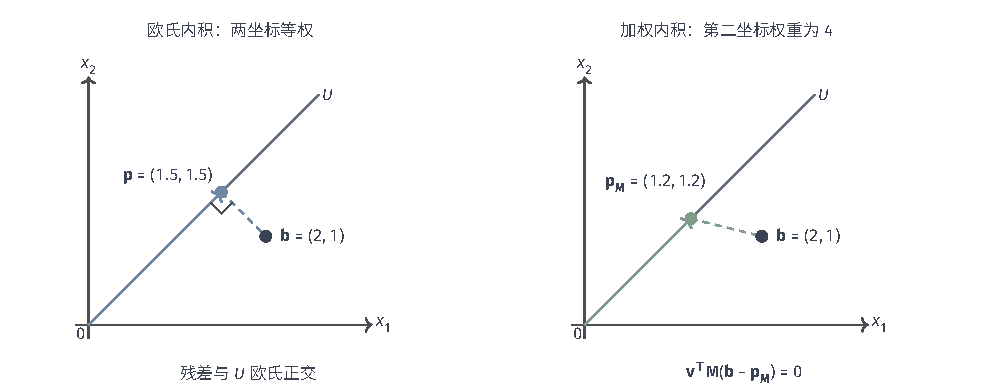
\includegraphics[width=168.998mm]{figures/00-shared/mathematical-preliminaries-upper/02-linear-spaces/tikz/linear-algebra-weighted-projection/figure.pdf}
  \caption{同一目标在同一直线上的欧氏投影与加权投影。实箭头是投影向量，虚线是残差；
  右图画在普通坐标中，残差不必形成欧氏直角。正交性必须用所选内积判断。}
  \label{fig:linear-algebra-weighted-projection}
\end{figure*}



加权问题可以化回普通问题。由定理~\ref{thm:ls-gram-factor}，正定$\bm M$可写成
$\bm M=\bm R^\top\bm R$，$\bm R$可逆。于是
$(\bm A\bm x-\bm b)^\top\bm M(\bm A\bm x-\bm b)=\lVert\bm R\bm A\bm x-\bm R\bm b\rVert_2^2$。
令$\tilde{\bm A}=\bm R\bm A$、$\tilde{\bm b}=\bm R\bm b$，加权目标就是普通平方残差$\lVert\tilde{\bm A}\bm x-\tilde{\bm b}\rVert_2^2$，
加权正规方程~\eqref{eq:linear-algebra-weighted-normal-equations}就是$\tilde{\bm A}^\top\tilde{\bm A}\hat{\bm x}=\tilde{\bm A}^\top\tilde{\bm b}$。
这一步常称\term{白化}（whitening）：先用$\bm R$把各坐标的误差变换到同一欧氏尺度。
于是前面的结论都可以搬过来：加权正规方程总有解；$\bm R$可逆使$\ker\tilde{\bm A}=\ker\bm A$，
所以解唯一的条件仍是$\bm A$满列秩。权重只移动最近点，不改变唯一性。

计算时把$\bm A,\bm b,\bm M$作为输入，先用Cholesky得到权重因子$\bm R$，再形成$\tilde{\bm A},\tilde{\bm b}$。对这对数据运行前面的QR或迭代最小二乘求解器，所得$\hat{\bm x}$就是原变量的解，无需再次变换未知量。输出时核验$\bm A^\top\bm M(\bm b-\bm A\hat{\bm x})$，并报告加权残差长度；普通残差的欧氏正交性已经不是这里的最优性条件。

\subsection{结果检验}
\label{sec:ls-least-squares-verification}

最小二乘的残差一般不为零，所以“残差小”不能作为合格标准；合格标准是残差与列空间正交。
算出$\hat{\bm x}$后分别核验三项。第一，正规方程残差$\bm g=\bm A^\top(\bm b-\bm A\hat{\bm x})$是否在容限内为零，
它检验的正是正交性判据。第二，输出残差$\bm r=\bm b-\bm A\hat{\bm x}$的长度，它是$\bm b$到列空间的距离，
说明模型能解释观测到什么程度。第三，若要求最小范数解，检查$\hat{\bm x}$是否与$\ker\bm A$正交。

用示例~\ref{ex:ls-normal-equations-three-by-two}核对：$\hat{\bm x}=(1,2)^\top$时$\bm r=(1,1,-1)^\top$，$\bm A^\top\bm r=(0,0)^\top$，第一项通过；
$\lVert\bm r\rVert_2=\sqrt3$，这是无法再减小的距离；$\bm A$满列秩，$\ker\bm A=\{\bm0\}$，第三项自动满足。

加权问题按原目标核验：检查加权正规方程~\eqref{eq:linear-algebra-weighted-normal-equations}的残差
$\bm A^\top\bm M(\bm b-\bm A\hat{\bm x})$，并报告$\bm M$加权的残差长度。白化后的残差（用$\bm M=\bm R^\top\bm R$的因子$\bm R$变换后的$\bm R\bm r$）与它长度相同，
但坐标已经变换，不能当作原观测的残差逐项解读。

\section{线性方程与最小二乘方法的比较}

前面的算法都围绕线性关系展开，但返回的对象并不相同。选择方法前，应先确定任务要求满足方程、最小化残差，还是在多个最优解中选出长度最小的一个；随后再检查矩阵结构和可用的数据访问方式。

\subsection{求解目标与方法适用性}

相容方程要求原残差为零。若零空间非平凡，这仍不能唯一决定未知量：从一个解加上任何零空间向量，输出都不变。最小范数要求解与零空间正交，是额外的选解条件。

不相容问题的原残差不能消失。欧氏最小二乘要求正规残差为零；如果又要求最小范数，还须使解位于行空间。因而“残差下降”“达到最小二乘解”和“得到最小范数解”是三种不同的判断，不能用同一个停止量代替。

\subsection{矩阵条件}

表中“矩阵作用”指能够计算矩阵与向量的乘积，不必保存整个矩阵。迭代法的条件指本章已经建立保证的情形；一般矩阵上的表现不能由方法名称保证。

\begin{center}
\small
\begin{tabular}{p{0.24\textwidth}p{0.65\textwidth}}
\toprule
方法 & 适用条件与主要输出\\
\midrule
LU & 可逆方阵；选主元消元后求精确方程的解\\
Cholesky & 对称正定方阵；分解可供多个右端复用\\
块LDL$^\top$ & 对称可逆矩阵，可含不定性；需要对称选主元\\
Schur补 & 已知分块且被消去的块可逆；先求约化方程\\
Woodbury & 已有可复用的基矩阵求解器，更新秩较低\\
Richardson & 对称正定时可按谱范围选步长；只用矩阵作用\\
Jacobi & 对角非零；严格行对角占优保证收敛，正定本身不够\\
Gauss--Seidel & 严格行对角占优或对称正定；逐行原位更新\\
SOR、SSOR & 对称正定且$0<\omega<2$；顺序扫掠或双向扫掠\\
CG & 对称正定；短递推，最小化能量范数误差\\
GMRES & 一般非奇异方阵；最小化原残差，需保存搜索基\\
MINRES & 对称非奇异方阵，可不定；最小化原残差\\
BiCG & 一般非对称方阵；需要矩阵及转置作用，可能失效\\
BiCGSTAB & 一般非对称方阵；无需转置作用，仍须检查失效\\
\bottomrule
\end{tabular}
\end{center}

矩形问题还需要比较求解目标。下面几种方法直接以最小二乘或行投影为出发点，不必先把原矩阵改成方阵。

\begin{center}
\small
\begin{tabular}{p{0.24\textwidth}p{0.65\textwidth}}
\toprule
方法 & 适用条件与主要输出\\
\midrule
正规方程法 & 满列秩最小二乘；形成正规矩阵会平方条件数\\
QR & 满列秩最小二乘；正交变换后求三角方程\\
SVD & 包括秩亏情形；给出秩、最小残差与最小范数代表\\
LSQR、LSMR & 矩形矩阵与转置作用；分别侧重原残差和正规残差\\
Kaczmarz & 相容系统，逐行访问；零初值选出最小范数解\\
扩展Kaczmarz & 允许不相容，需行列访问及辅助向量；概率保证另论\\
\bottomrule
\end{tabular}
\end{center}

左乘可逆矩阵保持精确方程的解集，却一般改变不相容问题中残差的权重。右换元保持可达到的输出，但欧氏最小范数随坐标尺度改变。把问题转换成某算法能够接收的形状以后，还要检查求解目标是否仍是原来的目标。

\subsection{计算开销与收敛速度}

稠密$n$阶LU、Cholesky、QR分解的工作量都为$O(n^3)$，因子的存储为$O(n^2)$；Cholesky利用对称性减少常数。分解完成后，每个新右端通常只需$O(n^2)$的三角求解。对$m\ge d$的稠密矩形矩阵，QR的主要工作量为$O(md^2)$。稀疏情形不能直接把这些估计中的维数换成非零元数，因为消元可能产生填充。

若矩阵有$s$个非零元，一次矩阵作用通常为$O(s)$。CG与BiCGSTAB等短递推保存常数个工作向量；完整GMRES的第$k$步还需对$k$个旧向量正交化，增加$O(kn)$工作和$O(kn)$存储。LSQR与LSMR每步使用一次矩阵作用和一次转置作用，工作向量总长度与$m+d$同阶。重正交化会改变这一存储估计。

因此总成本是每轮代价乘以达到要求所需的轮数，还要加上预条件构造和应用成本。只比较迭代次数，或只比较一次矩阵作用，都不足以判断哪个方法更省。

\subsection{数值稳定性}

正交变换避免了换基中的长度放大，因而QR常比显式形成正规方程更可靠；它仍不能消除原矩阵的小奇异值。SVD揭示这些方向，却也不能从带噪数据中恢复本来就不确定的分量。截断和惩罚会改变问题，应与单纯改善计算过程区别开来。

迭代结束时重新计算原残差。最小二乘还检查正规残差，并结合矩阵尺度解释容差。递推残差很小而真实残差较大，说明舍入误差已影响递推；相邻解几乎不变则可能只是停滞。若数据本身只精确到一定尺度，过度降低计算残差未必改善最终解。

\subsection{典型场景中的取舍}

对中等规模的稠密可逆方阵，可以从带选主元LU开始；若已知对称正定，改用Cholesky。多个右端共用矩阵时，复用分解通常比重复启动迭代更合适。已有分解而矩阵只发生低秩修改时，再检查Woodbury的小系统是否可逆、是否值得复用。

对大型稀疏对称正定系统，可以使用预条件CG；对称不定时考虑保持对称结构的MINRES。一般非对称系统中，GMRES用较多存储换取明确的残差最小化，BiCGSTAB用短递推减少存储，但需接受残差波动及失效检查。

对稠密矩形最小二乘，满列秩时可用QR；需要识别秩或最小范数时使用SVD。大型矩形问题若提供矩阵与转置作用，可用LSQR或LSMR；只方便逐行读取且系统相容时，行投影才直接符合数据访问方式。算法的选择由目标、结构与成本共同决定。


\section{伪逆}
\label{sec:ls-pseudoinverse}

到这里，三种情况各有各的答案。$\bm A$可逆时，唯一解是$\bm A^{-1}\bm b$；满行秩而有无穷多解时，
最小范数解是$\bm A^\top(\bm A\bm A^\top)^{-1}\bm b$；满列秩而无解时，最小二乘解是$(\bm A^\top\bm A)^{-1}\bm A^\top\bm b$。
三个公式各自要求一种满秩，而一般的$\bm A$可能既不满行秩、也不满列秩，这时方程可能无解，
最小二乘解又不唯一，需要先取最近点、再在最近点的全部原像中取范数最小者。
本小节用第~\ref{chap:linear-analysis}章的奇异值分解构造一个矩阵$\bm A^\dagger$，
使$\bm A^\dagger\bm b$在任何秩下都给出这样两次选择的结果，再说明前面三个公式都是它的特例。

\subsection{用SVD构造统一的解}

设$\bm A\in\mathbb R^{m\times d}$的秩为$r$，奇异值分解为~\eqref{eq:matrix-analysis-svd-rank-one-sum}，
$\sigma_1\geq\cdots\geq\sigma_r>0$；按第~\ref{sec:ls-svd}节的构造，把$\bm u_1,\ldots,\bm u_r$与$\bm v_1,\ldots,\bm v_r$
分别扩充为$\mathbb R^m$与$\mathbb R^d$的标准正交基。那里已经说明，$\operatorname{range}(\bm A)$由$\bm u_1,\ldots,\bm u_r$张成，
$\ker\bm A$由$\bm v_{r+1},\ldots,\bm v_d$张成。

$\bm A$把$\bm v_i$伸缩为$\sigma_i\bm u_i$，反向自然应把$\bm u_i$送回$\bm v_i/\sigma_i$。
按两次选择的要求分配$\bm b$的各个分量：把$\bm b$按$\bm u_i$展开，分量$\bm u_i^\top\bm b$（$i\leq r$）配给$\bm v_i/\sigma_i$；
落在$\operatorname{range}(\bm A)^\perp$中的分量（$i>r$）没有原像，直接丢弃，这对应取最近点；
零空间方向$\bm v_{r+1},\ldots,\bm v_d$不分配任何分量，这对应在原像中取范数最小者。

\begin{definition}[Moore--Penrose伪逆]
\label{def:matrix-analysis-pseudoinverse}
设$\bm A$有奇异值分解~\eqref{eq:matrix-analysis-svd-rank-one-sum}。$\bm A$的\term{Moore--Penrose伪逆}（Moore--Penrose pseudoinverse）为
\begin{equation}
 \bm A^\dagger=\sum_{i=1}^r\frac{1}{\sigma_i}\bm v_i\bm u_i^\top,
 \label{eq:matrix-analysis-pseudoinverse}
\end{equation}
$\bm A=\bm0$时规定$\bm A^\dagger=\bm0$。
\end{definition}

用于计算时不必先形成整个伪逆矩阵。输入$\bm A,\bm b$后，计算紧致SVD；对每个非零奇异值依次计算$c_i=\bm u_i^\top\bm b$与$z_i=c_i/\sigma_i$，最后组合$\hat{\bm x}=\sum_{i=1}^r z_i\bm v_i$。输出包含解及原残差；若数据只能确定数值秩，还要报告采用的阈值，因为丢掉正的小奇异值就转为后面的截断求解。

下面在精确秩已知的条件下，证明这样构造的矩阵恰好完成了上面的两次选择。
\begin{theorem}[最小二乘与最小范数]
\label{thm:matrix-analysis-pseudoinverse-minimum-norm}
给定$\bm A\in\mathbb R^{m\times d}$和$\bm b\in\mathbb R^m$，全部最小二乘解为
\begin{equation}
\begin{gathered}
\hat{\bm x}=\bm A^\dagger\bm b+\bm z\\
\bm z\in\ker\bm A,
\end{gathered}
\label{eq:ls-all-pseudoinverse-solutions}
\end{equation}
其中$\bm A^\dagger\bm b$是唯一的最小欧氏范数解；方程相容时，它就是全部精确解中范数最小者。
\end{theorem}
\begin{proof}
把$\bm b$与$\bm x$分别按左、右奇异向量展开，记$b_i=\bm u_i^\top\bm b$、$c_i=\bm v_i^\top\bm x$。由$\bm A\bm x=\sum_{i\leq r}\sigma_ic_i\bm u_i$与$\bm u_1,\ldots,\bm u_m$标准正交，
\[
 \lVert\bm A\bm x-\bm b\rVert_2^2
 =\sum_{i=1}^r(\sigma_ic_i-b_i)^2+\sum_{i=r+1}^m b_i^2 .
\]
第二项与$\bm x$无关；第一项当且仅当$c_i=b_i/\sigma_i$（$i\leq r$）时为零，而$c_{r+1},\ldots,c_d$可以任取。前者正是$\bm A^\dagger\bm b$的坐标，后者组成$\ker\bm A$中的任意向量，所以最小二乘解恰为$\bm A^\dagger\bm b+\bm z$，$\bm z\in\ker\bm A$。由于$\bm A^\dagger\bm b$只含$\bm v_1,\ldots,\bm v_r$方向，它与$\bm z$正交，$\lVert\bm x\rVert_2^2=\lVert\bm A^\dagger\bm b\rVert_2^2+\lVert\bm z\rVert_2^2$，最小值仅在$\bm z=\bm0$时达到。方程相容时第二项为零，最小二乘解就是精确解，论证不变。
\end{proof}

\paragraph{三种情况的统一}

定理对$\bm A$的秩和$\bm b$的位置都没有要求，所以前面分别处理的情况都包含在其中。
方程相容时，最近点就是$\bm b$本身，$\bm A^\dagger\bm b$是精确解中范数最小的一个：解唯一时它就是那个解，
有无穷多解时它就是第~\ref{sec:ls-select-among-solutions}节的最小范数解。方程无解时，$\bm A^\dagger\bm b$是最小二乘解；
最小二乘解唯一时它就是那一个，不唯一时它是其中范数最小者。

三个满秩公式由此成为特例。$\bm A$满列秩时$\ker\bm A=\{\bm0\}$，最小二乘解唯一，
所以对每个$\bm b$都有$\bm A^\dagger\bm b=(\bm A^\top\bm A)^{-1}\bm A^\top\bm b$，即$\bm A^\dagger=(\bm A^\top\bm A)^{-1}\bm A^\top$。
$\bm A$满行秩时每个右端都相容，$\bm A^\dagger\bm b$是最小范数精确解，由第~\ref{sec:ls-select-among-solutions}节，
$\bm A^\dagger=\bm A^\top(\bm A\bm A^\top)^{-1}$。$\bm A$可逆时两种情形同时成立，两个公式都化为$\bm A^{-1}$，所以$\bm A^\dagger=\bm A^{-1}$。
下面用一个欠定方程核对满行秩的情形。

\begin{example}[欠定方程的伪逆]
\label{ex:ls-pinv-underdetermined}
欠定方程$2x_1=3$的系数矩阵$\bm A=[2\ 0]$满行秩，右端$\bm b=(3)$。$\bm A$的奇异值分解只有一项：
$\sigma_1=2$、$\bm u_1=(1)$、$\bm v_1=(1,0)^\top$。和式~\eqref{eq:matrix-analysis-pseudoinverse}给出
\[
 \bm A^\dagger=\frac12\bm v_1\bm u_1^\top=\begin{bmatrix}1/2\\0\end{bmatrix},
\]
与满行秩公式$\bm A^\top(\bm A\bm A^\top)^{-1}=(2,0)^\top/4$一致。$\bm A^\dagger\bm b=(3/2,0)^\top$
正是全部解$(3/2,t)^\top$中范数最小的一个。
\end{example}

秩亏而又不相容时，两次选择都真正起作用，满秩公式一个也用不上。

\begin{example}[秩亏且不相容时的两次选择]
\label{ex:ls-pinv-two-selections}
取$\bm A=\left[\begin{smallmatrix}1&1\\0&0\end{smallmatrix}\right]$、$\bm b=(2,1)^\top$。$\bm A$的秩为$1$，既不满行秩，也不满列秩。
可达输出都形如$(s,0)^\top$，其中离$\bm b$最近的是$(2,0)^\top$，残差$(0,1)^\top$无法消除。
$(2,0)^\top$的原像是直线$x_1+x_2=2$，由示例~\ref{ex:ls-min-norm-line}，其上最靠近原点的点是$(1,1)^\top$。
用和式核对：$\bm A$只有一个正奇异值$\sigma_1=\sqrt2$，对应$\bm u_1=(1,0)^\top$、$\bm v_1=(1,1)^\top/\sqrt2$，于是
\[
\begin{gathered}
\bm A^\dagger=\frac1{\sqrt2}\bm v_1\bm u_1^\top=\frac12\begin{bmatrix}1&0\\1&0\end{bmatrix}\\
\bm A^\dagger\bm b=\begin{bmatrix}1\\1\end{bmatrix}.
\end{gathered}
\]
两次选择的结果与和式一致。
\end{example}

图~\ref{fig:matrix-analysis-pseudoinverse-selections}画出这两次选择。
伪逆既没有让无解的方程变得可解，也没有恢复被$\bm A$消去的信息，它只是在两处都作了最小化选择。

\begin{figure*}[htbp]
  \centering
  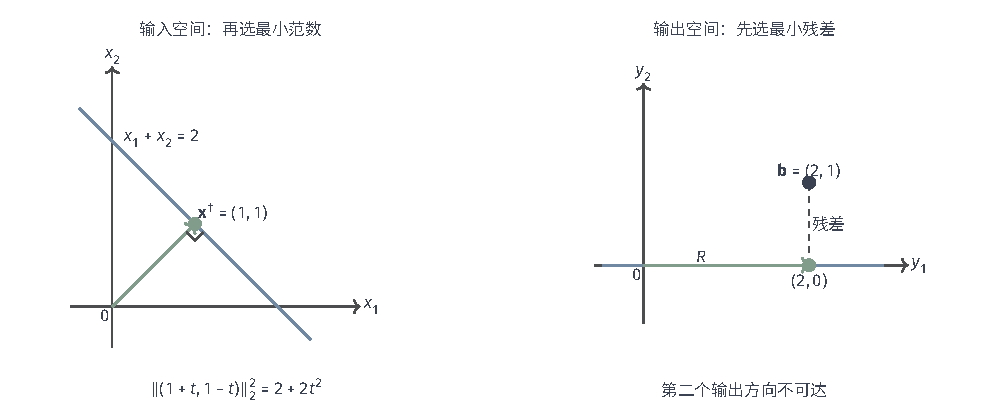
\includegraphics[width=168.998mm]{figures/00-shared/mathematical-preliminaries-upper/02-linear-spaces/tikz/matrix-analysis-pseudoinverse-selections/figure.pdf}
  \caption{伪逆的两次选择。右图先在可达输出中选择离$\bm b=(2,1)^\top$最近的
  $(2,0)^\top$；左图再在整条原像直线$x_1+x_2=2$上选择最靠近原点的$(1,1)^\top$。
  两图属于不同空间，各自等比例绘制。}
  \label{fig:matrix-analysis-pseudoinverse-selections}
\end{figure*}

\subsection{Penrose条件与两个投影}

两次选择也可以用投影矩阵表达。由和式直接相乘，
\[
 \begin{gathered}
\bm A\bm A^\dagger=\sum_{i\leq r}\bm u_i\bm u_i^\top\\
\bm A^\dagger\bm A=\sum_{i\leq r}\bm v_i\bm v_i^\top ,
 \end{gathered}
\]
前者是到$\operatorname{range}(\bm A)$的正交投影，后者是到$(\ker\bm A)^\perp=\operatorname{range}(\bm A^\top)$的正交投影
（式~\eqref{eq:linear-algebra-orthogonal-projector}）。也就是说，$\bm A^\dagger$先把输出正交投影到$\operatorname{range}(\bm A)$，
再在$\operatorname{range}(\bm A^\top)$上反演$\bm A$。

奇异值分解并不唯一，伪逆却不依赖分解的具体选取。由上面两个投影，$\bm A^\dagger$满足四条Penrose条件：
\[
 \begin{gathered}
\bm A\bm A^\dagger\bm A=\bm A\\
\bm A^\dagger\bm A\bm A^\dagger=\bm A^\dagger\\
(\bm A\bm A^\dagger)^\top=\bm A\bm A^\dagger\\
(\bm A^\dagger\bm A)^\top=\bm A^\dagger\bm A .
 \end{gathered}
\]
满足这四条的矩阵只有一个，所以无论用哪个奇异值分解代入和式，得到的都是同一个矩阵。

下面证明唯一性。

设$\bm G$也满足四条条件。由第一条，$(\bm A\bm G)^2=(\bm A\bm G\bm A)\bm G=\bm A\bm G$，即$\bm A\bm G$幂等，
且$\operatorname{range}(\bm A\bm G)=\operatorname{range}(\bm A)$（$\subseteq$显然，$\supseteq$由$\bm A=\bm A\bm G\bm A$）；
同理$\bm G\bm A$幂等，且$\ker(\bm G\bm A)=\ker\bm A$（$\supseteq$显然，$\subseteq$由$\bm A=\bm A\bm G\bm A$）。
后两条说明它们对称，而由第~\ref{sec:ls-projection-matrices}节，对称的幂等矩阵就是到其像的正交投影。
$\bm A\bm G$与$\bm A\bm A^\dagger$都是到$\operatorname{range}(\bm A)$的正交投影，所以$\bm A\bm G=\bm A\bm A^\dagger$。
对称矩阵的像是其零空间的正交补，所以$\bm G\bm A$与$\bm A^\dagger\bm A$都是到$(\ker\bm A)^\perp$的正交投影，$\bm G\bm A=\bm A^\dagger\bm A$。再由第二条，
\[
 \bm G=\bm G\bm A\bm G=(\bm A^\dagger\bm A)\bm G=\bm A^\dagger(\bm A\bm G)=\bm A^\dagger\bm A\bm A^\dagger=\bm A^\dagger .
\]

至此，三种情况的答案统一为$\bm A^\dagger\bm b$。实际计算中，满秩时仍用前面各小节基于分解的方法，
不必为此计算奇异值分解；伪逆的作用在于给出一个对任何秩都成立的统一描述。

不过伪逆有一个与逆矩阵不同的性质：它关于矩阵不连续。非零标量$\varepsilon$的伪逆是$1/\varepsilon$，零的伪逆却是$0$，
$\varepsilon\to0$时前者趋于无穷，而不是趋于后者。原因在于和式中的增益$1/\sigma_i$：小奇异值被放大成大增益。
数据带有误差时，这种放大意味着什么，是下一节要回答的问题。

\section{方程与最小二乘的误差分析}
\label{sec:ls-numerical-sensitivity}

前面各小节都假定$\bm A$与$\bm b$精确，并在精确算术下求解。实际数据带有测量误差，计算又有舍入误差，
所以还要问：输入有一点误差时，算出的解会偏离多少？残差小时，解是否就准确？
第~\ref{chap:linear-analysis}章已经回答了最简单的情形：可逆方程只有右端带误差时，
解的相对误差不超过条件数$\kappa(\bm A)$乘右端的相对误差（定理~\ref{thm:matrix-analysis-condition-number-bound}），
而在欧氏范数下$\kappa_2(\bm A)$是最大与最小奇异值之比。本节从这里出发，先处理系数矩阵也带误差的情形，
再说明真解未知时怎样由残差判断算出的解，然后分析最小二乘的三类输出。分析会显示，误差放大的根源都在小奇异值，
求解方法还可能额外放大误差；最后据此介绍数据与计算两方面的改进。

\subsection{右端项与系数矩阵的有限扰动}
\label{sec:ls-equation-sensitivity}
\label{sec:ls-linear-system-sensitivity}

\paragraph{右端扰动}

先看只改右端的情形。

设$\bm A$可逆，右端由$\bm b$变为$\bm b+\Delta\bm b$，解的变化为$\Delta\bm x=\bm A^{-1}\Delta\bm b$。
由$\lVert\bm A^{-1}\rVert_2=1/\sigma_{\min}(\bm A)$，右端误差落在小奇异值方向时被放大$1/\sigma_{\min}$倍；
换成相对误差，放大倍数不超过$\kappa(\bm A)$。下面用两个$2\times2$例子对照。

\begin{example}[良态方程的右端扰动]
\label{ex:ls-rhs-perturbation-well-conditioned}
取$\bm A_1=\operatorname{diag}(2,1)$，$\kappa_2(\bm A_1)=2$。右端由$(2,1)^\top$改为$(2,1.01)^\top$，解由$(1,1)^\top$变为$(1,1.01)^\top$。
两者的相对变化分别为
\[
 \begin{gathered}
\frac{\lVert\Delta\bm b\rVert_2}{\lVert\bm b\rVert_2}=\frac{0.01}{\sqrt5}\approx0.00447\\
\frac{\lVert\Delta\bm x\rVert_2}{\lVert\bm x\rVert_2}=\frac{0.01}{\sqrt2}\approx0.00707,
 \end{gathered}
\]
放大约$1.58$倍，不超过$\kappa_2(\bm A_1)=2$。
\end{example}

\begin{example}[近平行列的右端扰动]
\label{ex:ls-rhs-perturbation-near-parallel}
取$\bm A_2=\left[\begin{smallmatrix}1&1\\0&\varepsilon\end{smallmatrix}\right]$，$0<\varepsilon\ll1$，两列接近同向。
$\bm A_2^\top\bm A_2=\left[\begin{smallmatrix}1&1\\1&1+\varepsilon^2\end{smallmatrix}\right]$的迹为$2+\varepsilon^2$、行列式为$\varepsilon^2$，
两个特征值约为$2$与$\varepsilon^2/2$，所以$\sigma_{\max}\approx\sqrt2$、$\sigma_{\min}\approx\varepsilon/\sqrt2$，$\kappa_2(\bm A_2)\approx2/\varepsilon$。

取$\varepsilon=10^{-2}$、$\bm b=(2,0)^\top$，解为$(2,0)^\top$。只把$\bm b$的第二分量改为$\eta=10^{-2}$，
由$\varepsilon x_2=\eta$与$x_1+x_2=2$得新解$(1,1)^\top$。两者的相对变化分别为
\[
 \begin{gathered}
\frac{\lVert\Delta\bm b\rVert_2}{\lVert\bm b\rVert_2}=\frac{\eta}{2}=0.005\\
\frac{\lVert\Delta\bm x\rVert_2}{\lVert\bm x\rVert_2}=\frac{\lVert(-1,1)^\top\rVert_2}{\lVert(2,0)^\top\rVert_2}=\frac{\sqrt2}{2}\approx0.707,
 \end{gathered}
\]
放大约$141$倍，与$\kappa_2(\bm A_2)\approx200$同量级。
\end{example}

两个例子都没有舍入误差，差别完全来自问题本身。第二例中解的变化$(-1,1)^\top$几乎正沿着$\bm A_2$的小奇异值方向，
所以被放大得最多。

\paragraph{逆矩阵的扰动}
\label{sec:ls-inverse-sensitivity}
\label{sec:ch06-inverse-stability}

$\bm A$本身也带误差时，扰动后的矩阵甚至可能不再可逆。所以设$\bm B=\bm A+\bm E$，要先回答两件事：
$\bm B$是否可逆，$\bm B^{-1}$离$\bm A^{-1}$多远。答案会给出一个“到奇异边界的余量”。

先看可逆性。若$\lVert\bm A^{-1}\bm E\rVert<1$，则$\bm B$可逆。假设$\bm B\bm x=\bm0$，即$\bm A\bm x=-\bm E\bm x$，左乘$\bm A^{-1}$得$\bm x=-\bm A^{-1}\bm E\bm x$，取范数得$\lVert\bm x\rVert\leq\lVert\bm A^{-1}\bm E\rVert\lVert\bm x\rVert$，这只在$\bm x=\bm0$时可能，所以$\ker\bm B=\{\bm0\}$。

再看逆的变化。由$\bm B^{-1}(\bm A-\bm B)\bm A^{-1}=\bm B^{-1}-\bm A^{-1}$，逆差满足精确恒等式
\begin{equation}
 \bm B^{-1}-\bm A^{-1}
 =-\bm B^{-1}\bm E\,\bm A^{-1}.
 \label{eq:ch06-inverse-finite-perturbation}
\end{equation}
右端含有未知的$\bm B^{-1}$，需要先估计它的大小。

对任意$\bm y$，令$\bm x=\bm B^{-1}\bm y$，由$\bm A\bm x=\bm y-\bm E\bm x$得$\bm x=\bm A^{-1}\bm y-\bm A^{-1}\bm E\bm x$，取范数并移项，$\lVert\bm x\rVert\leq\lVert\bm A^{-1}\rVert\lVert\bm y\rVert/(1-\lVert\bm A^{-1}\bm E\rVert)$，即
\[
 \lVert\bm B^{-1}\rVert\leq\frac{\lVert\bm A^{-1}\rVert}{1-\lVert\bm A^{-1}\bm E\rVert}.
\]
代入恒等式，$\lVert\bm B^{-1}-\bm A^{-1}\rVert\leq\lVert\bm B^{-1}\rVert\lVert\bm E\rVert\lVert\bm A^{-1}\rVert$。两边除以$\lVert\bm A^{-1}\rVert$，并用$\lVert\bm A^{-1}\bm E\rVert\leq\lVert\bm A^{-1}\rVert\lVert\bm E\rVert=\kappa(\bm A)\lVert\bm E\rVert/\lVert\bm A\rVert$。为了用这个较易计算的上界替换分母，还需假设$\kappa(\bm A)\lVert\bm E\rVert/\lVert\bm A\rVert<1$；在此条件下得到
\[
 \frac{\lVert\bm B^{-1}-\bm A^{-1}\rVert}
      {\lVert\bm A^{-1}\rVert}
 \leq
 \frac{\kappa(\bm A)\,\lVert\bm E\rVert/\lVert\bm A\rVert}
      {1-\kappa(\bm A)\,\lVert\bm E\rVert/\lVert\bm A\rVert}.
\]
分子是条件数乘相对扰动，分母是到奇异边界的余量。$\kappa(\bm A)\lVert\bm E\rVert/\lVert\bm A\rVert$接近$1$时界急剧变大；
它不小于$1$时本界失效，但这不等于$\bm B$一定奇异。下面的对角例子说明，这个界可以取等号，余量趋于零时逆矩阵的变化确实无界。

\begin{example}[接近奇异边界的对角矩阵]
\label{ex:ls-inverse-perturbation-diagonal}
取$\bm A=\operatorname{diag}(1,\varepsilon)$，$0<\varepsilon<1$，则$\kappa_2(\bm A)=1/\varepsilon$。
令$\bm E=\operatorname{diag}(0,-\delta)$，$0<\delta<\varepsilon$，即把第二个对角元减少$\delta$。
逆矩阵的该元由$1/\varepsilon$变为$1/(\varepsilon-\delta)$，相对变化为
\[
 \frac{\lVert\bm B^{-1}-\bm A^{-1}\rVert_2}{\lVert\bm A^{-1}\rVert_2}
 =\frac{1/(\varepsilon-\delta)-1/\varepsilon}{1/\varepsilon}
 =\frac{\delta}{\varepsilon-\delta}.
\]
扰动的相对大小为$\lVert\bm E\rVert_2/\lVert\bm A\rVert_2=\delta$，于是$\kappa_2(\bm A)\lVert\bm E\rVert_2/\lVert\bm A\rVert_2=\delta/\varepsilon$，
上界为$(\delta/\varepsilon)/(1-\delta/\varepsilon)=\delta/(\varepsilon-\delta)$，与实际变化恰好相等。
$\delta\to\varepsilon$时相对变化无界：扰动的相对大小接近$1/\kappa_2(\bm A)=\varepsilon$时，矩阵到达奇异边界。
\end{example}

\paragraph{矩阵与右端同时扰动}

有了逆矩阵的估计，就可以处理一般情形。

设$\bm A$可逆且$\bm b\ne\bm0$，原解$\bm x$因而非零。扰动后的方程为$(\bm A+\bm E)(\bm x+\Delta\bm x)=\bm b+\Delta\bm b$，减去$\bm A\bm x=\bm b$，得$\bm A\Delta\bm x=\Delta\bm b-\bm E\bm x-\bm E\Delta\bm x$。左乘$\bm A^{-1}$并取范数，
\[
 \lVert\Delta\bm x\rVert\leq\lVert\bm A^{-1}\rVert\bigl(\lVert\Delta\bm b\rVert+\lVert\bm E\rVert\lVert\bm x\rVert+\lVert\bm E\rVert\lVert\Delta\bm x\rVert\bigr).
\]
把含$\lVert\Delta\bm x\rVert$的项移到左边，两边除以$\lVert\bm x\rVert$，并用$\lVert\Delta\bm b\rVert/\lVert\bm x\rVert\leq\lVert\bm A\rVert\lVert\Delta\bm b\rVert/\lVert\bm b\rVert$，在$\kappa(\bm A)\lVert\bm E\rVert/\lVert\bm A\rVert<1$时得到
\begin{equation}
 \frac{\lVert\Delta\bm x\rVert}{\lVert\bm x\rVert}
 \leq
 \frac{\kappa(\bm A)}{1-\kappa(\bm A)\lVert\bm E\rVert/\lVert\bm A\rVert}
 \left(
 \frac{\lVert\Delta\bm b\rVert}{\lVert\bm b\rVert}
 +\frac{\lVert\bm E\rVert}{\lVert\bm A\rVert}
 \right).
 \label{eq:matrix-analysis-linear-system-perturbation}
\end{equation}
读法是：两类相对扰动先相加，再被条件数放大，最后除以到奇异边界的余量。
$\bm E=\bm0$时它退回定理~\ref{thm:matrix-analysis-condition-number-bound}的右端扰动界。
这仍是最坏方向上的上界；扰动是否落在放大方向，决定实际误差离这个上界有多远。

\subsection{残差、前向误差与后向误差}
\label{sec:ls-numerical-stability}
\label{sec:ls-data-computation-error}
\label{sec:linear-algebra-error-propagation}
\label{sec:ch06-error-propagation}
\label{sec:ls-result-verification}
\label{sec:matrix-analysis-error-verification}

上面的界比较的是两个精确解。实际手里只有一个算出的候选解$\widehat{\bm x}$，真解未知，怎样判断它的误差？以下仍设$\bm A$可逆且$\bm b\ne\bm0$。
第~\ref{sec:ls-linear-equation-verification}节用残差核验候选解，并提醒残差小不等于解准确；现在可以定量说明这一点。能直接计算的是残差
\begin{equation}
 \bm r=\bm b-\bm A\widehat{\bm x}.
 \label{eq:matrix-analysis-residual}
\end{equation}
由$\bm A(\bm x-\widehat{\bm x})=\bm r$，候选解的误差是$\bm A^{-1}\bm r$，与只改右端的情形相同，相对误差满足
\[
 \frac{\lVert\widehat{\bm x}-\bm x\rVert}{\lVert\bm x\rVert}
 \leq\kappa(\bm A)\frac{\lVert\bm r\rVert}{\lVert\bm b\rVert}.
\]
所以病态时小残差不保证解准确，下面的例子把这一点推到极端。

\begin{example}[反例：残差小而解误差大]
\label{ex:ls-small-residual-large-error}
取$\bm A=\operatorname{diag}(1,\varepsilon)$、$\bm b=(1,\varepsilon)^\top$，$0<\varepsilon\ll1$，精确解为$\bm x=(1,1)^\top$。
候选解$\widehat{\bm x}=(1,0)^\top$的残差为$\bm r=(0,\varepsilon)^\top$，相对残差为$\varepsilon/\sqrt{1+\varepsilon^2}$，随$\varepsilon\to0$趋于零；
相对解误差却是$\lVert(0,-1)^\top\rVert_2/\lVert(1,1)^\top\rVert_2=1/\sqrt2$，不随$\varepsilon$减小。
这与上面的界一致：$\kappa_2(\bm A)=1/\varepsilon$恰好抵消了相对残差中的因子$\varepsilon$。
\end{example}

残差还有另一种读法：把$\widehat{\bm x}$看作某个邻近问题的精确解，问这个邻近问题离原问题多近。
满足$(\bm A+\Delta\bm A)\widehat{\bm x}=\bm b+\Delta\bm b$的最小相对扰动称为\term{后向误差}（backward error）；
与之相对，直接比较答案的误差$\widehat{\bm x}-\bm x$称为\term{前向误差}（forward error）。
允许矩阵与右端同时改变、以相对大小$\max\{\lVert\Delta\bm A\rVert_2/\lVert\bm A\rVert_2,\lVert\Delta\bm b\rVert_2/\lVert\bm b\rVert_2\}$度量时，后向误差为
\begin{equation}
 \eta_2(\widehat{\bm x})
 =\frac{\lVert\bm r\rVert_2}
       {\lVert\bm A\rVert_2\lVert\widehat{\bm x}\rVert_2+\lVert\bm b\rVert_2}.
 \label{def:matrix-analysis-normwise-backward-error}
\end{equation}
先说明它不能更小：若$(\bm A+\Delta\bm A)\widehat{\bm x}=\bm b+\Delta\bm b$且两项相对大小都不超过$\epsilon$，则$\bm r=\Delta\bm A\widehat{\bm x}-\Delta\bm b$，
$\lVert\bm r\rVert_2\leq\epsilon(\lVert\bm A\rVert_2\lVert\widehat{\bm x}\rVert_2+\lVert\bm b\rVert_2)$，即$\epsilon\geq\eta_2$。
再说明它能达到。若$\widehat{\bm x}=\bm0$，取$\Delta\bm A=\bm0$、$\Delta\bm b=-\bm b$即可达到$\eta_2=1$。

若$\widehat{\bm x}\ne\bm0$，记分母为$d_0$，取
\[
 \begin{gathered}
\Delta\bm A=\frac{\lVert\bm A\rVert_2}{d_0\lVert\widehat{\bm x}\rVert_2}\,\bm r\widehat{\bm x}^\top\\
\Delta\bm b=-\frac{\lVert\bm b\rVert_2}{d_0}\,\bm r ,
 \end{gathered}
\]
则$(\bm A+\Delta\bm A)\widehat{\bm x}=\bm b-\bm r+\tfrac{\lVert\bm A\rVert_2\lVert\widehat{\bm x}\rVert_2}{d_0}\bm r=\bm b+\Delta\bm b$，两项的相对大小都等于$\eta_2$。

把后向误差当作式~\eqref{eq:matrix-analysis-linear-system-perturbation}中的数据扰动，就得到常用的经验规则：
前向误差大约不超过条件数乘后向误差。

后向误差的用处在于把算法的质量与问题的病态分开。计算机中的实数运算都有舍入，每次基本运算满足
\begin{equation}
\begin{gathered}
\operatorname{fl}(x\circ y)=(x\circ y)(1+\delta)\\
|\delta|\leq u,
\end{gathered}
\label{eq:ch06-floating-point-model}
\end{equation}
其中$\circ$是加减乘除之一，$u$称为单位舍入，双精度时$u=2^{-53}\approx1.1\times10^{-16}$。这个模型假设运算有定义且结果没有发生溢出或影响相对误差界的下溢。好的算法应当让这些舍入合起来只相当于一个很小的输入扰动。

\begin{definition}[后向稳定]
\label{def:matrix-analysis-backward-stability}
若算法对所有合法输入给出的结果都是某个邻近输入的精确解，且后向误差以$u$乘一个与数据无关的温和常数为界，则称算法\term{后向稳定}（backward stable）。
\end{definition}
正定矩阵的Cholesky分解与Householder QR（第~\ref{sec:ls-orthogonalization-qr}节）具有后向稳定性。带部分主元的LU分解，其后向误差界还依赖消元中的元素增长；增长温和时通常稳定，但不能对所有矩阵保证这个因子都很小。

示例~\ref{ex:ls-partial-pivoting}中不选主元的消元可能产生很大的乘子，把舍入误差放大成很大的输入扰动。

后向稳定只保证$\widehat{\bm x}$是邻近问题的精确解；病态问题中，很小的后向误差经条件数放大，仍可能得到很大的前向误差。
稳定算法不能治愈问题本身的病态，所以报告结果时要同时给出残差或后向误差，以及条件数的估计。

\subsection{最小二乘的不同输出与正规方程的风险}
\label{sec:ls-ls-regularization-sensitivity}
\label{sec:ls-ordinary-ls-sensitivity}

最小二乘有三类输出：系数$\hat{\bm x}=\bm A^\dagger\bm b$、拟合值$\bm A\hat{\bm x}=\bm P_{\operatorname{range}\bm A}\bm b$与残差$\bm b-\bm A\hat{\bm x}$。
它们对扰动的反应不同。

设$\bm A$固定、右端改变$\Delta\bm b$。拟合值的增量是$\bm P_{\operatorname{range}\bm A}\Delta\bm b$，正交投影不放大长度；
残差增量是$(\bm I-\bm P_{\operatorname{range}\bm A})\Delta\bm b$，同样不被放大；系数的增量却是$\bm A^\dagger\Delta\bm b$，
由伪逆的和式，$\lVert\Delta\hat{\bm x}\rVert_2\leq\lVert\Delta\bm b\rVert_2/\sigma_r$，其中$\sigma_r$是最小正奇异值；若$\bm A=\bm0$，伪逆为零，系数的增量也为零。
所以“拟合得好”与“系数可靠”是两回事，不能用一个误差数概括。

\paragraph{近共线设计}

示例~\ref{ex:ls-nearly-collinear-design}显示，拟合可以很好而系数很大。下面用奇异值说明原因。

\begin{example}[近共线设计的奇异值]
\label{ex:ls-nearly-collinear-singular-values}
示例~\ref{ex:ls-nearly-collinear-design}中设计矩阵$\bm X_\varepsilon$的两列是$\bm c_1$与$\bm c_1+\varepsilon\bm q$，
其中$\bm c_1=(1,1,1)^\top$、$\bm q=(0,1,-1)^\top$互相正交，所以两列都位于$\operatorname{span}\{\bm c_1,\bm q\}$内。
以$\bm c_1/\sqrt3$、$\bm q/\sqrt2$为这个平面的正交坐标，两列的坐标分别是$(\sqrt3,0)^\top$与$(\sqrt3,\sqrt2\,\varepsilon)^\top$；
再把全部输出统一除以$\sqrt3$，设计矩阵化为
\begin{equation}
\begin{gathered}
\bm X_{\widetilde\varepsilon}
 =\begin{bmatrix}1&1\\0&\widetilde\varepsilon\end{bmatrix}\\
\widetilde\varepsilon=\sqrt{2/3}\,\varepsilon .
\end{gathered}
\label{eq:matrix-analysis-nearly-collinear-design}
\end{equation}
换成正交坐标不改变奇异值，统一缩放只把奇异值同除以$\sqrt3$，不改变它们的比，所以条件数可以在$\bm X_{\widetilde\varepsilon}$上计算。

Gram矩阵$\bm X_{\widetilde\varepsilon}^\top\bm X_{\widetilde\varepsilon}=\left[\begin{smallmatrix}1&1\\1&1+\widetilde\varepsilon^2\end{smallmatrix}\right]$的迹为$2+\widetilde\varepsilon^2$，
行列式为$\widetilde\varepsilon^2$，特征值为
\begin{equation}
 \lambda_\pm
 =\frac{2+\widetilde\varepsilon^2
          \mathbin{\pm}\sqrt{4+\widetilde\varepsilon^4}}{2}.
 \label{eq:matrix-analysis-nearly-collinear-gram-eigenvalues}
\end{equation}
$\widetilde\varepsilon\to0$时$\lambda_+\to2$，$\lambda_-=\widetilde\varepsilon^2/\lambda_+\approx\widetilde\varepsilon^2/2$，
所以$\bm X_{\widetilde\varepsilon}$的奇异值$\sigma_{\max}\to\sqrt2$、$\sigma_{\min}\approx\widetilde\varepsilon/\sqrt2$，
条件数约为$2/\widetilde\varepsilon=\sqrt6/\varepsilon$。乘回$\sqrt3$，$\bm X_\varepsilon$本身的最小奇异值约为$\sqrt3\,\widetilde\varepsilon/\sqrt2=\varepsilon$。
\end{example}

大奇异值对应的方向近似为两个系数同增同减，小奇异值对应的方向近似为两个系数此增彼减。
响应在后一方向上的分量被放大约$1/\varepsilon$倍，这正是$\hat{\bm w}_\varepsilon$中$\delta/\varepsilon$项的来源。

化简后的$\bm X_{\widetilde\varepsilon}$与示例~\ref{ex:ls-rhs-perturbation-near-parallel}的近平行矩阵$\bm A_2$形状相同，
所以可以在$\bm A_2$上直接看到系数怎样分裂。

\begin{example}[近平行列的系数分裂]
\label{ex:ls-coefficient-splitting}
沿用示例~\ref{ex:ls-rhs-perturbation-near-parallel}的$\bm A_2=\left[\begin{smallmatrix}1&1\\0&\varepsilon\end{smallmatrix}\right]$，
把右端扰动写成一般的$\eta$。右端为$(2,0)^\top$时解为$(2,0)^\top$；右端变为$(2,\eta)^\top$时，由$\varepsilon x_2=\eta$与$x_1+x_2=2$得
\begin{equation}
\begin{gathered}
\hat{\bm x}=\begin{bmatrix}2-\eta/\varepsilon\\ \eta/\varepsilon\end{bmatrix}\\
\Delta\hat{\bm x}=\begin{bmatrix}-\eta/\varepsilon\\ \eta/\varepsilon\end{bmatrix}.
\end{gathered}
\label{eq:matrix-analysis-collinear-coefficient-perturbation}
\end{equation}
系数误差的长度$\sqrt2\,|\eta|/\varepsilon$是右端误差$|\eta|$的$\sqrt2/\varepsilon$倍，两个系数沿相反方向分开。
$\bm A_2$可逆，拟合值始终等于右端本身。
\end{example}

图~\ref{fig:matrix-analysis-coefficient-sensitivity}画出$\varepsilon$减小时两个系数怎样分开。

\begin{figure}
 \centering
 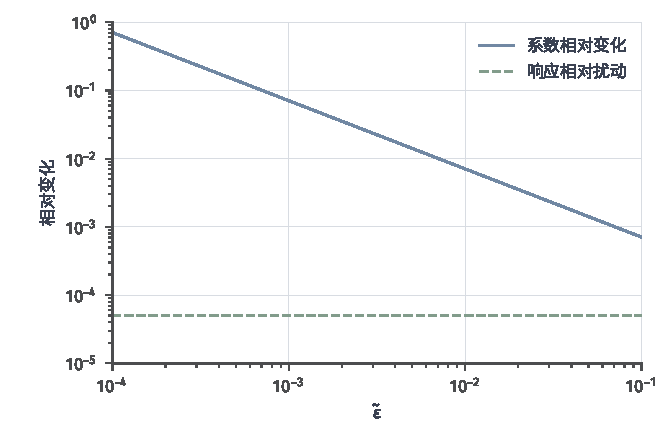
\includegraphics[width=0.92\linewidth]{figures/00-shared/mathematical-preliminaries-upper/02-linear-spaces/matplotlib/matrix-analysis-coefficient-sensitivity/figure.pdf}
 \caption{近平行列的系数分裂：对$\bm A_2=\left[\begin{smallmatrix}1&1\\0&\varepsilon\end{smallmatrix}\right]$固定右端扰动$\eta$，$\varepsilon$越小，两个系数
 沿相反方向偏离$(2,0)$越远，绝对误差随$1/\varepsilon$增长。}
 \label{fig:matrix-analysis-coefficient-sensitivity}
\end{figure}

\paragraph{正规方程的条件数平方}

问题本身的敏感度之外，求解方法也会影响结果。由奇异值分解，$\bm A^\top\bm A$的特征值是$\sigma_i^2$，故满列秩时
\begin{equation}
 \kappa_2(\bm A^\top\bm A)=\kappa_2(\bm A)^2.
 \label{eq:matrix-analysis-normal-equation-condition-square}
\end{equation}
平方的后果在近平行矩阵上看得最清楚。

\begin{example}[形成Gram矩阵时丢失的信息]
\label{ex:ls-gram-rounding-loss}
对示例~\ref{ex:ls-rhs-perturbation-near-parallel}的$\bm A_2$，$\kappa_2(\bm A_2)\approx2/\varepsilon$。
Gram矩阵$\bm A_2^\top\bm A_2=\left[\begin{smallmatrix}1&1\\1&1+\varepsilon^2\end{smallmatrix}\right]$的小特征值约为$\varepsilon^2/2$，条件数约为$4/\varepsilon^2$。
取$\varepsilon=10^{-8}$，则$\varepsilon^2=10^{-16}$已低于双精度的单位舍入$u\approx1.1\times10^{-16}$，
$1+\varepsilon^2$在舍入后就是$1$，存储下来的Gram矩阵成为奇异的$\left[\begin{smallmatrix}1&1\\1&1\end{smallmatrix}\right]$。
而$\bm A_2$本身的条件数约为$2\times10^8$，远未达到$1/u$，它的两列在双精度下仍可区分。
\end{example}

所以形成$\bm A^\top\bm A$这一步就可能把小奇异方向的信息丢掉。这就是第~\ref{sec:ls-qr-method}节的QR方法不形成$\bm A^\top\bm A$的原因：
用Householder反射实现时（第~\ref{sec:ls-orthogonalization-qr}节），它只经过正交变换，不会在问题本身的敏感度之外再把条件数平方。

\subsection{伪逆、秩变化与数值秩}

以上只改右端。矩阵本身改变时，秩是否保持起决定作用。设$\bm A$与$\bm B=\bm A+\bm E$的正奇异值都不小于$s_0>0$。
直接展开右端可验证恒等式
\[
 \bm B^\dagger-\bm A^\dagger
 =-\bm B^\dagger\bm E\bm A^\dagger
 +\bm B^\dagger(\bm I-\bm A\bm A^\dagger)
 -(\bm I-\bm B^\dagger\bm B)\bm A^\dagger .
\]
三项分别估计。非零矩阵满足$\lVert\bm A^\dagger\rVert_2=1/\sigma_r(\bm A)\leq1/s_0$；零矩阵的伪逆也是零，仍满足这个上界。对$\bm B$同理。
第一项不超过$\lVert\bm B^\dagger\rVert_2\lVert\bm E\rVert_2\lVert\bm A^\dagger\rVert_2\leq\lVert\bm E\rVert_2/s_0^2$。
第二项利用Penrose条件写$\bm B^\dagger=\bm B^\dagger(\bm B\bm B^\dagger)^\top=\bm B^\dagger(\bm B^\dagger)^\top\bm B^\top$；
又因$\bm A^\top(\bm I-\bm A\bm A^\dagger)=\bm0$，有$\bm B^\top(\bm I-\bm A\bm A^\dagger)=\bm E^\top(\bm I-\bm A\bm A^\dagger)$，
所以该项不超过$\lVert\bm B^\dagger\rVert_2^2\lVert\bm E\rVert_2\leq\lVert\bm E\rVert_2/s_0^2$。第三项同理。合起来，
\begin{equation}
 \lVert\bm B^\dagger-\bm A^\dagger\rVert_2
 \leq\frac{3\lVert\bm E\rVert_2}{s_0^2}.
 \label{eq:ch06-pseudoinverse-fixed-rank-perturbation}
\end{equation}
这个估计本身不要求两矩阵同秩，关键是它们的正奇异值有共同的正下界。若一列矩阵趋于$\bm A$而秩在极限处下降，就会有正奇异值趋于零，此时不能使用与扰动无关的$s_0$。相反，在固定秩且正奇异值远离零的邻域内，上界直接给出伪逆的连续性。

\begin{example}[反例：秩改变时伪逆不连续]
\label{ex:ls-pinv-discontinuity}
取$\bm A=\operatorname{diag}(1,0)$与$\bm B_\varepsilon=\operatorname{diag}(1,\varepsilon)$，$0<\varepsilon<1$。
二者之差$\lVert\bm B_\varepsilon-\bm A\rVert_2=\varepsilon\to0$，但
\[
 \begin{gathered}
\bm B_\varepsilon^\dagger=\operatorname{diag}(1,1/\varepsilon)\\
\bm A^\dagger=\operatorname{diag}(1,0),
 \end{gathered}
\]
所以$\lVert\bm B_\varepsilon^\dagger-\bm A^\dagger\rVert_2=1/\varepsilon\to\infty$。
$\bm B_\varepsilon$的秩为$2$，$\bm A$的秩为$1$；两者正奇异值的公共下界只能取$s_0=\varepsilon$，
界~\eqref{eq:ch06-pseudoinverse-fixed-rank-perturbation}给出$3\varepsilon/\varepsilon^2=3/\varepsilon$，同样随$\varepsilon\to0$无界。
\end{example}

这将伪逆一节末尾的标量现象扩展到了矩阵，也说明秩变化时新出现的小奇异值为何危险。

实际数据的秩因而要谨慎对待。第~\ref{chap:linear-analysis}章的奇异值扰动界~\eqref{eq:matrix-analysis-singular-value-perturbation}说明，矩阵改变$\bm E$时每个奇异值的移动不超过$\lVert\bm E\rVert_2$，所以小于数据误差尺度的奇异值与零无法区分：它可能是一个真实但很弱的方向，也可能只是噪声。据此，把大于某个阈值$\tau$的奇异值个数称为\term{数值秩}（numerical rank），$\tau$按数据误差的尺度选取。

综合本小节的分析：无论是方程的解、最小二乘的系数还是伪逆本身，误差放大都来自小奇异值。
它们一方面使增益$1/\sigma_i$很大，另一方面在误差尺度下难以与零区分；形成正规方程之类的计算步骤还会进一步损失精度。
前面的QR等方法避免额外引入不稳定计算；下一节转向正则化，通过改变目标来限制数据误差的放大。

\section{正则化与截断求解}
\label{sec:ls-truncated-svd-ridge}

小奇异值会把右端误差放大到解中。提高计算精度只能减少计算误差，不能消除数据本身的不确定性。本节通过限制小奇异值方向上的响应来换取稳定，同时明确所求的问题已发生改变。

\subsection{岭回归与Tikhonov正则化}
\label{sec:ls-regularized-ls}

示例~\ref{ex:ls-nearly-collinear-design}中，系数为了拟合上的微小改进而取得很大。若任务希望输入不要太大，
可以在数据项之外加上输入长度的平方惩罚，得到\term{岭回归}（ridge regression）
\begin{equation}
\begin{gathered}
\min_{\bm x}\ \lVert\bm A\bm x-\bm b\rVert_2^2+\lambda\lVert\bm x\rVert_2^2\\
\lambda>0.
\end{gathered}
\label{eq:ls-ridge-objective}
\end{equation}
参数$\lambda$权衡两项：$\lambda$越大，越倾向于小的输入，拟合误差不会减小；在某些退化情形下它也可能保持不变。

更一般地，惩罚可以作用在希望压小的量$\bm L\bm x$上，$\bm L\in\mathbb R^{p\times d}$，例如相邻分量之差，
得到\term{Tikhonov正则化}（Tikhonov regularization）\scite{math-hansen2008regtools}
\begin{equation}
\begin{gathered}
\min_{\bm x}\ \lVert\bm A\bm x-\bm b\rVert_2^2+\lambda\lVert\bm L\bm x\rVert_2^2\\
\lambda>0.
\end{gathered}
\label{eq:linear-algebra-general-tikhonov}
\end{equation}
两项都是平方长度，而$\lambda\lVert\bm L\bm x\rVert_2^2=\lVert\sqrt\lambda\,\bm L\bm x-\bm0\rVert_2^2$，
所以可以把两个残差向量上下堆成一个更长的残差向量，写成堆叠矩阵的普通最小二乘，
称为\term{增广最小二乘}（augmented least squares）：
\begin{equation}
 \begin{bmatrix}\bm A\\ \sqrt{\lambda}\,\bm L\end{bmatrix}\bm x
 \approx\begin{bmatrix}\bm b\\ \bm0\end{bmatrix}.
 \label{eq:ls-augmented-system}
\end{equation}
对堆叠矩阵套用正规方程~\eqref{eq:linear-algebra-normal-equations}：堆叠矩阵的转置乘自身是
$\bm A^\top\bm A+\lambda\bm L^\top\bm L$，转置乘堆叠右端是$\bm A^\top\bm b$，于是
\begin{equation}
 (\bm A^\top\bm A+\lambda\bm L^\top\bm L)\hat{\bm x}=\bm A^\top\bm b.
 \label{eq:ls-tikhonov-normal}
\end{equation}
它是普通最小二乘，存在性自动成立。由~\eqref{eq:ls-normal-kernel}，系数矩阵的零空间就是堆叠矩阵的零空间，
即同时满足$\bm A\bm x=\bm0$与$\bm L\bm x=\bm0$的向量，所以解唯一当且仅当
\begin{equation}
 \ker\bm A\cap\ker\bm L=\{\bm0\}.
 \label{eq:linear-algebra-tikhonov-common-nullspace}
\end{equation}
$\bm L=\bm I$时条件自动成立，岭回归对任意$\bm A$都有唯一解。其他惩罚则未必。

\begin{example}[反例：惩罚无法确定的方向]
\label{ex:ls-tikhonov-common-nullspace}
取$\bm A=\bm L=[\,1\ -1\,]$。两者的零空间都是$\operatorname{span}\{(1,1)^\top\}$，条件~\eqref{eq:linear-algebra-tikhonov-common-nullspace}不成立。
对任何解$\hat{\bm x}$和任何$t\in\mathbb R$，$\hat{\bm x}+t(1,1)^\top$的数据项与惩罚项都不变，因而也是解。
所以无论$\lambda$多大，都不能确定两个分量的共同水平。
\end{example}

权重与惩罚也可以同时使用，目标
$(\bm A\bm x-\bm b)^\top\bm M(\bm A\bm x-\bm b)+\lambda\lVert\bm L\bm x\rVert_2^2$的正规方程为
\begin{equation}
 (\bm A^\top\bm M\bm A+\lambda\bm L^\top\bm L)\hat{\bm x}=\bm A^\top\bm M\bm b,
 \label{eq:ls-general-normal-equations}
\end{equation}
$\bm M$正定、$\lambda>0$时，解唯一的条件仍是~\eqref{eq:linear-algebra-tikhonov-common-nullspace}。
要注意，加惩罚改变的是问题本身：选择$\lambda$是在重新设定任务，而不是让原方程“算得出来”的数值技巧。

$\lambda$怎样影响解，可以在奇异值坐标中读出。岭回归的正规方程是$(\bm A^\top\bm A+\lambda\bm I)\bm x=\bm A^\top\bm b$。在右奇异向量坐标$c_i=\bm v_i^\top\bm x$中，
$\bm A^\top\bm A$与$\bm I$同时成为对角矩阵，方程按方向分开：$i\leq r$时$(\sigma_i^2+\lambda)c_i=\sigma_i\,\bm u_i^\top\bm b$，
$i>r$时$\lambda c_i=0$，故$c_i=0$。于是
\begin{equation}
\begin{gathered}
\hat{\bm x}_\lambda=\sum_{i=1}^r\frac{\sigma_i}{\sigma_i^2+\lambda}\,(\bm u_i^\top\bm b)\,\bm v_i
 =\sum_{i=1}^r f_i\,\frac{\bm u_i^\top\bm b}{\sigma_i}\,\bm v_i\\
f_i=\frac{\sigma_i^2}{\sigma_i^2+\lambda}.
\end{gathered}
\label{eq:matrix-analysis-ridge-filter-factor}
\end{equation}
前一种写法说明，岭回归把伪逆中的增益$1/\sigma_i$换成了$\sigma_i/(\sigma_i^2+\lambda)$。由$\sigma_i^2+\lambda\geq2\sigma_i\sqrt\lambda$，
新的增益不超过$1/(2\sqrt\lambda)$，不再随$\sigma_i\to0$而爆炸。

后一种写法把它与最小范数解比较：每个方向多乘了一个介于$0$与$1$之间的\term{滤波因子}（filter factor）$f_i$。
$\sigma_i^2\gg\lambda$时$f_i\approx1$，该方向几乎不受影响；$\sigma_i^2\ll\lambda$时$f_i\approx\sigma_i^2/\lambda$，该方向被压低，增益约为$\sigma_i/\lambda$；
$\sigma_i^2=\lambda$处$f_i$恰为$1/2$。代价是大奇异值方向也被轻微压缩，$f_i$总小于$1$。下面在近共线设计上看两个$\lambda$的效果。

\begin{example}[近共线设计上的岭回归]
\label{ex:ls-ridge-nearly-collinear}
沿用示例~\ref{ex:ls-nearly-collinear-design}的$\bm X_\varepsilon$与$\bm y$，取$\varepsilon=0.01$、$\delta=0.1$。
直接计算可得两个奇异值约为$\sigma_1\approx2.449$、$\sigma_2\approx0.0100$，
对应的右奇异向量近似为$(1,1)^\top/\sqrt2$与$(1,-1)^\top/\sqrt2$。精确最小二乘解是$(-9,10)^\top$，残差为零；
它的大系数全部来自第二个方向，该方向的系数$\bm u_2^\top\bm y/\sigma_2$的绝对值约为$0.134/0.0100\approx13.4$。
按式~\eqref{eq:matrix-analysis-ridge-filter-factor}计算两个$\lambda$下的结果：
\[
 \begin{array}{cccc}
  \lambda & f_2 & \hat{\bm x}_\lambda & \lVert\bm X_\varepsilon\hat{\bm x}_\lambda-\bm y\rVert_2\\[2pt]
  10^{-4} & \approx0.50 & \approx(-4.25,\,5.25)^\top & \approx0.067\\
  10^{-2} & \approx0.0099 & \approx(0.41,\,0.59)^\top & \approx0.133
 \end{array}
\]
$\lambda=10^{-4}\approx\sigma_2^2$时，第二个方向保留一半；$\lambda=10^{-2}$时，第二个方向几乎被去掉。
第一个方向的因子$f_1$在两种情形下都大于$0.998$。所以随着$\lambda$增大，解从精确拟合的大系数逐渐移向两个系数平分共同作用的解，
代价是残差增大。
\end{example}

计算岭回归不必作奇异值分解，上面的滤波因子只用于解释$\lambda$的作用。正规方程$(\bm A^\top\bm A+\lambda\bm I)\hat{\bm x}=\bm A^\top\bm b$的系数矩阵对任意$\bm A$都正定，
可以用Cholesky分解；更可靠的做法是对堆叠矩阵~\eqref{eq:ls-augmented-system}作QR分解，避免形成$\bm A^\top\bm A$。
一般的Tikhonov惩罚（$\bm L\neq\bm I$）不能由$\bm A$一个矩阵的奇异值分解按方向分开，但同样可以用堆叠矩阵的QR分解求解。

这给出统一的计算步骤：输入$\bm A,\bm b,\bm L$与选定的$\lambda>0$，组成增广系数$\bm F=[\bm A^\top\;\sqrt\lambda\bm L^\top]^\top$和增广右端$\bm c=(\bm b^\top,\bm0^\top)^\top$。若公共零空间为零，对$\bm F$作经济型QR分解$\bm F=\bm Q_F\bm R_F$，计算$\bm g=\bm Q_F^\top\bm c$，回代$\bm R_F\hat{\bm x}_\lambda=\bm g$。公共零空间非零时，改用SVD并声明选择最小范数解。整个过程输出的是正则化目标的解，不能再用原来无惩罚的正规残差为零作为验收条件。

核验时要回到原目标，分别报告数据项$\lVert\bm A\hat{\bm x}-\bm b\rVert_2^2$（加权时为$\bm M$加权长度）、惩罚项$\lambda\lVert\bm L\hat{\bm x}\rVert_2^2$
以及正规方程~\eqref{eq:ls-general-normal-equations}的残差，不能只报告堆叠问题的残差。

\subsection{截断SVD求解}

这里的输入除$\bm A,\bm b$外，还包括保留阶数$k$或奇异值阈值$\tau$。

先将奇异值按降序排列，再保留前$k$个方向；若用阈值，则令$k$等于满足$\sigma_i>\tau$的个数。对保留方向计算$c_i=\bm u_i^\top\bm b$、$z_i=c_i/\sigma_i$，再组合输出。没有方向被保留时输出零向量。

这里$k$表示保留阶数，不是迭代次数；后面的$\bm x_k$是这一阶数对应的截断解。

岭回归按滤波因子连续地压低小奇异值方向。更直接的做法是只在前$k$个奇异方向上反演，丢弃其余方向：
\[
\begin{gathered}
\bm x_k=\sum_{i=1}^k\frac{\bm u_i^\top\bm b}{\sigma_i}\,\bm v_i\\
1\leq k\leq r ,
\end{gathered}
\]
相当于滤波因子只取$1$（$i\leq k$）或$0$（$i>k$）。$k=r$时它就是$\bm A^\dagger\bm b$；$k<r$时，它恰是把$\bm A$换成第~\ref{sec:ls-svd}节的截断SVD$\bm A_k=\sum_{i\leq k}\sigma_i\bm u_i\bm v_i^\top$
（式~\eqref{eq:matrix-analysis-truncated-svd}）后，所得问题的最小范数最小二乘解，即$\bm x_k=\bm A_k^\dagger\bm b$。
由Eckart--Young--Mirsky定理~\ref{thm:matrix-analysis-best-low-rank}，$\bm A_k$是离$\bm A$最近的秩$k$矩阵，
所以截断SVD解相当于先用最接近的低秩矩阵代替$\bm A$，再精确地解代替后的问题。

收益与代价都可以从坐标中直接读出。收益是放大倍数受控：观测误差对$\bm x_k$的影响至多被放大$1/\sigma_k$倍，
而不是$1/\sigma_r$倍。代价是残差增加：被丢弃方向上的观测分量不再被拟合，平方残差比原最小二乘问题多出
$\sum_{i=k+1}^r(\bm u_i^\top\bm b)^2$。若这些分量主要来自噪声，丢弃它们正是所求；若其中含有真实信号，信号也一并丢失。
$k$取多大，取决于哪些奇异值可以与零区分：取$k$为数值秩，就是只在可信的方向上反演。下面仍用近共线设计说明。

\begin{example}[近共线设计上的截断SVD]
\label{ex:ls-tsvd-nearly-collinear}
沿用示例~\ref{ex:ls-ridge-nearly-collinear}的数据与奇异值分解，取$k=1$，只保留第一个奇异方向：
\[
 \bm x_1=\frac{\bm u_1^\top\bm y}{\sigma_1}\,\bm v_1\approx(0.50,\,0.50)^\top .
\]
两个系数平分共同的作用。残差长度约为$0.134$，即被丢弃的分量$|\bm u_2^\top\bm y|$，接近响应中$\delta\bm q$部分的长度$\delta\sqrt2\approx0.141$。
$\lambda=10^{-2}$时的岭回归解$(0.41,0.59)^\top$已经接近它。
\end{example}

截断以后，拟合不再精确，但系数不再随$\delta/\varepsilon$而爆炸。

截断SVD需要奇异值分解，适合规模不大、或需要逐个检查奇异值的情形。

$k$与$\lambda$都不是由方程本身确定的量。它们决定在多大程度上用拟合误差换取解的稳定，
应当按任务对两者的要求、以及数据误差的尺度来选择；常见的办法是比较不同参数下残差与解的大小\scite{math-hansen2008regtools}，
或在留出的数据上检验预测效果。无论用哪种办法，报告结果时都应说明所用的$k$或$\lambda$，因为它们改变的是所解的问题。

% 矩阵方程：西尔维斯特（Sylvester）方程AX+XB=C（线性算子、可逆性、求解：一般情况与可对角情况）；
% 李雅普诺夫（Lyapunov）方程AX+XA^T=Q与离散型X-A^TXA=Q（可解性与对称性、求解、正定性与离散级数解）；本章小结

\section{西尔维斯特方程}
\label{sec:ls-matrix-equations}
\label{sec:linear-algebra-matrix-equations}

上一节的未知量是向量。本节和下一节的未知量本身是一张矩阵，已知矩阵从左边、右边或两边乘在它上面，
这样的方程称为\term{矩阵方程}（matrix equation）。本节的主角是西尔维斯特（Sylvester）方程：
未知矩阵分别受到左乘与右乘，两种作用相加。我们回答三个问题：方程表达什么，
何时有解、何时唯一，以及怎样求解。

\subsection{矩阵未知量与线性算子}
\label{sec:ls-matrix-equation-types}

最简单的矩阵方程只从一侧作用。单侧方程$\bm A\bm X=\bm C$就是上一节的多右端方程：左乘$\bm A$对$\bm X$的每一列
做同一个线性变换。类似地，右乘对每一行做同一个线性变换。双侧方程$\bm A\bm X\bm B=\bm C$同时受两侧约束。
本节的重点是两侧作用相加的情形。

\begin{definition}[Sylvester方程]
\label{def:matrix-analysis-sylvester-equation}
给定$\bm A\in\mathbb R^{m\times m}$、$\bm B\in\mathbb R^{n\times n}$、$\bm C\in\mathbb R^{m\times n}$，
求$\bm X\in\mathbb R^{m\times n}$使
\[
 \bm A\bm X+\bm X\bm B=\bm C .
\]
这一方程称为\term{Sylvester方程}（Sylvester equation）。
\end{definition}

方程的左边是$\bm X$的函数$\mathcal L(\bm X)=\bm A\bm X+\bm X\bm B$，它把$\mathbb R^{m\times n}$映到自身。
由矩阵乘法的分配律，$\mathcal L(\alpha\bm X_1+\beta\bm X_2)=\alpha\mathcal L(\bm X_1)+\beta\mathcal L(\bm X_2)$，
所以$\mathcal L$是$mn$维空间$\mathbb R^{m\times n}$上的线性算子，Sylvester方程就是线性方程$\mathcal L(\bm X)=\bm C$。
上一节关于线性方程的结论因此全部适用。特别地，$\mathcal L$把一个空间映到同维的自身，
由秩零度定理，它对每个$\bm C$都有唯一解，当且仅当齐次方程$\mathcal L(\bm X)=\bm0$只有零解。

\paragraph{向量化与Kronecker表示}

为了真正套用上一节的工具，可以把矩阵拉直成向量。第~\ref{sec:ls-kronecker-products}节的向量化恒等式
$\operatorname{vec}(\bm A\bm X\bm B)=(\bm B^\top\otimes\bm A)\operatorname{vec}\bm X$
把矩阵乘积写成Kronecker积作用于向量。对$\bm A\bm X=\bm A\bm X\bm I_n$取$\bm B=\bm I_n$，
对$\bm X\bm B=\bm I_m\bm X\bm B$取$\bm A=\bm I_m$，两式相加，Sylvester方程化为
\begin{equation}
 (\bm I_n\otimes\bm A+\bm B^\top\otimes\bm I_m)\operatorname{vec}\bm X
 =\operatorname{vec}\bm C.
 \label{eq:ls-sylvester-vectorized}
\end{equation}
这是一个$mn$阶的普通线性方程。双侧方程同理化为$(\bm B^\top\otimes\bm A)\operatorname{vec}\bm X=\operatorname{vec}\bm C$。
于是第~\ref{sec:ls-solution-cases}节的相容性判据与解集结构都可以直接用在矩阵方程上。

\subsection{存在唯一性的谱条件}
\label{sec:ls-matrix-equation-existence}

单侧和双侧方程可以直接沿用列空间的判据。单侧方程$\bm A\bm X=\bm C$相容，当且仅当$\bm C$的每一列都在$\operatorname{range}\bm A$中，
即$\operatorname{rank}[\bm A\ \bm C]=\operatorname{rank}\bm A$。双侧方程$\bm A\bm X\bm B=\bm C$的左边，每一列都是$\bm A$的列的组合，
每一行都是$\bm B$的行的组合，所以相容的必要条件是$\operatorname{range}\bm C\subseteq\operatorname{range}\bm A$
且$\operatorname{range}\bm C^\top\subseteq\operatorname{range}\bm B^\top$；完整的判据是向量化方程的增广秩条件。
$\bm A,\bm B$都可逆时，两侧分别乘逆，得唯一解$\bm X=\bm A^{-1}\bm C\bm B^{-1}$。任一侧秩亏时，不能写出这个公式：
方程可能无解，有解时解还可以沿该侧的零空间变动，不唯一。

Sylvester方程的两项相加，情况不同：可解性不取决于$\bm A$、$\bm B$各自是否可逆，而取决于二者的特征值如何搭配。
下面先从对角情形看出这一点，再给出一般结论。

\paragraph{对角情形}

设$\bm A$与$\bm B$都是对角矩阵，对角元分别为$a_{i,i}$与$b_{j,j}$。$\bm A\bm X$把$\bm X$的第$i$行乘以$a_{i,i}$，
$\bm X\bm B$把第$j$列乘以$b_{j,j}$，所以$(\bm A\bm X+\bm X\bm B)_{i,j}=(a_{i,i}+b_{j,j})x_{i,j}$。
方程按元素分解成$mn$个互不相关的标量方程$(a_{i,i}+b_{j,j})x_{i,j}=c_{i,j}$，
只要每个分母非零，就有唯一解
\begin{equation}
 x_{i,j}=\frac{c_{i,j}}{a_{i,i}+b_{j,j}}.
 \label{eq:ls-sylvester-diagonal-closed-form}
\end{equation}
若某一对满足$a_{i,i}+b_{j,j}=0$，该位置的方程退化为$0\cdot x_{i,j}=c_{i,j}$：$c_{i,j}\neq0$时无解，$c_{i,j}=0$时该元素可任意取值。

对角元就是特征值，所以对角情形下，方程对每个$\bm C$唯一可解的条件是：$\bm A$的任一特征值与$\bm B$的任一特征值之和都不为零，
也就是$\bm A$的特征值与$-\bm B$的特征值互不相同。这个条件与$\bm A$、$\bm B$各自是否可逆无关，两个方向都有例子。

\begin{example}[反例：可解性不取决于各自可逆]
\label{ex:ls-sylvester-invertibility-irrelevant}
取$\bm A=\bm0\in\mathbb R^{m\times m}$、$\bm B=\bm I_n$。$\bm A$不可逆，但方程化为$\bm X=\bm C$，对每个$\bm C$唯一可解；
这里$\bm A$的特征值只有$0$，$-\bm B$的特征值只有$-1$，二者分离。

反过来，取$m=n=1$、$\bm A=2$、$\bm B=-2$，两者都可逆，方程却化为$(2-2)x=c$，即$0\cdot x=c$：
$c\neq0$时无解，$c=0$时任意$x$都是解。这里$2+(-2)=0$，分离条件不成立。
\end{example}

图~\ref{fig:ls-sylvester-separation}把这一分离条件画在实轴上。

\begin{figure}[htbp]
  \centering
  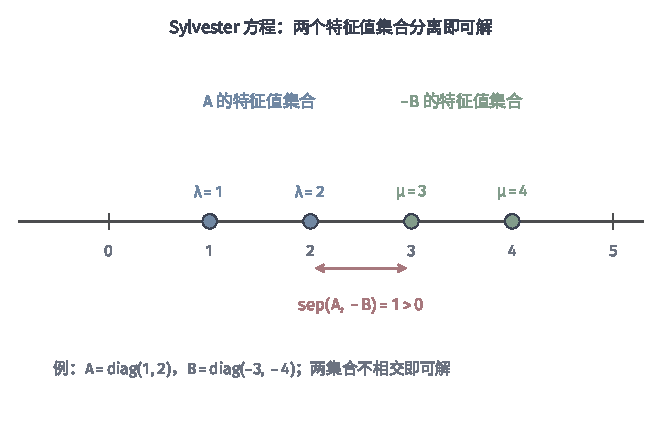
\includegraphics[width=112mm]{figures/00-shared/mathematical-preliminaries-upper/02-linear-spaces/matplotlib/ls-sylvester-separation/ls-sylvester-separation.pdf}
  \caption{Sylvester方程$\bm A\bm X+\bm X\bm B=\bm C$的特征值分离条件。
  $\bm A=\operatorname{diag}(1,2)$的特征值$\{1,2\}$与$-\bm B$（$\bm B=\operatorname{diag}(-3,-4)$）
  的特征值$\{3,4\}$在实轴上彼此分离，最近一对间距$|2-3|=1>0$，
  两集合不相交，故对任意$\bm C$有唯一解。只用实轴，不引入复数对象。}
  \label{fig:ls-sylvester-separation}
\end{figure}

\paragraph{Sylvester算子的可逆性}

一般情形的结论与对角情形相同。Sylvester算子$\mathcal L(\bm X)=\bm A\bm X+\bm X\bm B$可逆，当且仅当
\begin{equation}
\begin{gathered}
\lambda_i(\bm A)+\lambda_j(\bm B)\neq0
 \quad\text{对所有 }i,j\\
\text{即}\qquad
 \operatorname{spec}(\bm A)\cap\operatorname{spec}(-\bm B)=\varnothing,
\end{gathered}
\label{eq:ch06-sylvester-spectral-separation}
\end{equation}
其中$\operatorname{spec}$表示全体特征值，包括复特征值。实矩阵的特征值可能是复数（第~\ref{sec:ls-general-square-spectrum}节），所以条件要对全体特征值检查。

证明中会用到复特征向量。这样做是允许的：$\mathcal L$可逆等价于Kronecker矩阵~\eqref{eq:ls-sylvester-vectorized}的行列式非零，
而行列式不论在实数域还是复数域中计算都是同一个数，所以在复数域中证明齐次方程只有零解，也就证明了实算子可逆。

必要性。设条件不成立，即有$\bm A\bm u=\lambda\bm u$（$\bm u\neq\bm0$），且$-\lambda$是$\bm B$的特征值。
$\bm B^\top$与$\bm B$的特征多项式相同（$\det(\bm B^\top-\mu\bm I)=\det(\bm B-\mu\bm I)$），
所以存在$\bm w\neq\bm0$使$\bm B^\top\bm w=-\lambda\bm w$，即$\bm w^\top\bm B=-\lambda\bm w^\top$。
取$\bm X=\bm u\bm w^\top$，它不是零矩阵，而
\[
 \bm A\bm X+\bm X\bm B=(\bm A\bm u)\bm w^\top+\bm u(\bm w^\top\bm B)
 =\lambda\bm u\bm w^\top-\lambda\bm u\bm w^\top=\bm0 .
\]
齐次方程有非零解，算子不可逆。

充分性。设条件成立，且$\mathcal L(\bm X)=\bm0$，要证$\bm X=\bm0$。思路是找一个多项式$q$，
使$q(\bm A)=\bm0$而$q(-\bm B)$可逆，再利用二者与$\bm X$的关系。

第一步，把$\bm X$在两侧之间“搬运”。由$\bm A\bm X=\bm X(-\bm B)$，
得$\bm A^2\bm X=\bm A\bm X(-\bm B)=\bm X(-\bm B)^2$，归纳得$\bm A^k\bm X=\bm X(-\bm B)^k$；
对各次幂作线性组合，对任意多项式$q$有$q(\bm A)\bm X=\bm X\,q(-\bm B)$。

第二步，取$q$为$\bm A$的特征多项式$p_{\bm A}(z)=\det(z\bm I-\bm A)$。由Cayley--Hamilton定理~\ref{thm:ls-cayley-hamilton}，
$p_{\bm A}(\bm A)=\bm0$。在复数域中分解$p_{\bm A}(z)=\prod_k(z-\lambda_k)$，其中$\lambda_k$取遍$\bm A$的全部特征值，则
$p_{\bm A}(-\bm B)=\prod_k(-\bm B-\lambda_k\bm I)$。由条件~\eqref{eq:ch06-sylvester-spectral-separation}，
每个$\lambda_k$都不是$-\bm B$的特征值，所以每个因子$-\bm B-\lambda_k\bm I$都可逆，$p_{\bm A}(-\bm B)$作为可逆矩阵的乘积也可逆。

合起来，$\bm X\,p_{\bm A}(-\bm B)=p_{\bm A}(\bm A)\bm X=\bm0$，右乘$p_{\bm A}(-\bm B)^{-1}$得$\bm X=\bm0$。齐次方程只有零解，算子可逆。

至此，Sylvester方程是否对每个右端都有唯一解，完全由$\bm A$与$-\bm B$的特征值是否分离决定。
条件不成立时，方程对有些右端无解、对另一些右端有无穷多解，齐次解$\bm u\bm w^\top$给出了解不唯一的方向。

\subsection{基于Schur分解的求解}
\label{sec:ls-matrix-equation-solve}

本节统一输入$\bm A\in\mathbb R^{m\times m}$、$\bm B\in\mathbb R^{n\times n}$和$\bm C\in\mathbb R^{m\times n}$，输出满足$\bm A\bm X+\bm X\bm B=\bm C$的$\bm X$，并假定前面的谱分离条件成立。这里未知量有$mn$个元素，各方法只改变它们的组织方式；比较时应使用同一个原方程的Frobenius残差。

求解方法按$\bm A$、$\bm B$的结构分两种情况。一般情况下，方程可以化为普通线性方程直接求解，
但规模大时要用实Schur形把它约化成准三角形再逐块回代；$\bm A$、$\bm B$可对角化时，换到特征向量坐标后方程按元素分开，直接写出解。

\label{sec:ls-one-sided-two-sided}

\paragraph{向量化直接求解}

最直接的做法是形成系数矩阵~\eqref{eq:ls-sylvester-vectorized}，用第~\ref{sec:ls-direct-methods}节的LU分解求解。

具体说，按列堆叠$\bm C$得到$\bm c=\operatorname{vec}(\bm C)$，形成$\bm K=\bm I_n\otimes\bm A+\bm B^\top\otimes\bm I_m$，用带主元LU解$\bm K\bm z=\bm c$，再把$\bm z$按每$m$个元素一列还原成$\bm X$。这一步还原必须与向量化的顺序一致。
小规模问题这样做是可靠的，但系数矩阵有$(mn)^2$个元素，稠密LU约需$2(mn)^3/3$次运算；
$m=n=100$时系数矩阵已有$10^8$个元素。所以要尽量利用方程的结构，避免形成这个大矩阵。

单侧和双侧方程很容易做到。$\bm A\bm X=\bm C$是同一系数矩阵的多右端问题，对$\bm A$分解一次即可逐列复用。
双侧方程在$\bm A,\bm B$可逆时，先解$\bm A\bm Y=\bm C$，再解$\bm X\bm B=\bm Y$（即$\bm B^\top\bm X^\top=\bm Y^\top$），
也不形成Kronecker矩阵。双侧方程不相容时，可以改求$\min_{\bm X}\lVert\bm A\bm X\bm B-\bm C\rVert_{\mathrm F}^2$，
它是系数矩阵为$\bm B^\top\otimes\bm A$的最小二乘问题，由第~\ref{sec:ls-least-squares}节的方法求解。
Sylvester方程的两项相加，不能这样逐侧处理，下面借助$\bm A$、$\bm B$的正交相似变换。

\paragraph{实Schur约化}
\label{sec:ls-sylvester-schur}

正交变换不放大误差，而且由第~\ref{sec:ls-general-square-spectrum}节的实Schur形（定理~\ref{thm:ls-real-schur}），
任何实方阵都可以用正交相似化为接近三角的形状：$\bm A=\bm Q\bm T\bm Q^\top$，
$\bm Q$正交，$\bm T$是实准上三角矩阵，即对角线上是$1\times1$块（实特征值）或$2\times2$块（一对共轭复特征值），
对角块以下全为零。

分别取$\bm A=\bm Q\bm T\bm Q^\top$、$\bm B=\bm U\bm S\bm U^\top$，方程两边左乘$\bm Q^\top$、右乘$\bm U$，
利用$\bm Q^\top\bm A=\bm T\bm Q^\top$与$\bm B\bm U=\bm U\bm S$，并记$\bm Y=\bm Q^\top\bm X\bm U$、$\bm D=\bm Q^\top\bm C\bm U$，方程化为
\begin{equation}
 \bm T\bm Y+\bm Y\bm S=\bm D.
 \label{eq:ls-sylvester-transformed}
\end{equation}
正交相似不改变特征值，所以可逆条件不变；正交变换也不改变Frobenius范数，所以新坐标下的残差大小与原坐标相同。

\paragraph{准三角块上的逐块回代}

$\bm T$、$\bm S$不是对角的，方程不能按元素完全分开，但三角结构允许逐块依次求解，正如上三角方程可以回代。
按$\bm T$、$\bm S$的对角块把$\bm Y$、$\bm D$分块，比较第$(i,j)$块：
$(\bm T\bm Y)_{i,j}=\sum_k\bm T_{i,k}\bm Y_{k,j}$中只有$k\geq i$的项非零，
$(\bm Y\bm S)_{i,j}=\sum_\ell\bm Y_{i,\ell}\bm S_{\ell,j}$中只有$\ell\leq j$的项非零。
把含$\bm Y_{i,j}$的两项留在左边，其余移到右边：
\begin{equation}
 \bm T_{i,i}\bm Y_{i,j}+\bm Y_{i,j}\bm S_{j,j}
 =\bm D_{i,j}-\sum_{k>i}\bm T_{i,k}\bm Y_{k,j}
          -\sum_{\ell<j}\bm Y_{i,\ell}\bm S_{\ell,j}.
 \label{eq:ls-sylvester-block-recurrence}
\end{equation}
右边只用到同一列中更靠下的块$\bm Y_{k,j}$（$k>i$）和同一行中更靠左的块$\bm Y_{i,\ell}$（$\ell<j$）。
因此按列从左到右、每列从下到上的次序计算，每次右边需要的块都已求出。左边是一个小的Sylvester方程：
两个对角块都是$1\times1$时，它就是标量方程，直接除以$t_{i,i}+s_{j,j}$；含$2\times2$块时，它至多含$4$个未知量，
向量化后系数矩阵为$\bm I\otimes\bm T_{i,i}+\bm S_{j,j}^\top\otimes\bm I$。小块的特征值是$\bm A$、$\bm B$特征值的一部分，
由谱分离条件，每个小方程都唯一可解。

全部块求出后，由$\bm X=\bm Q\bm Y\bm U^\top$恢复原坐标，并在原坐标中计算残差$\bm A\bm X+\bm X\bm B-\bm C$。这一方法称为Bartels--Stewart算法。

两次实Schur约化的代价为$O(m^3+n^3)$，逐块回代的代价为$O(mn(m+n))$，远小于向量化直接求解的$O(m^3n^3)$；
约化只做一次，多个右端$\bm C$可以复用。

用一个已经为上三角形的例子观察回代次序。取
\[
 \bm A=\begin{bmatrix}1&1\\0&2\end{bmatrix},\qquad
 \bm B=\begin{bmatrix}3&1\\0&4\end{bmatrix},\qquad
 \bm C=\begin{bmatrix}7&12\\15&21\end{bmatrix}.
\]
此时正交因子都是单位矩阵，$\bm Y=\bm X$、$\bm D=\bm C$。按第一列从下到上计算，得到
\begin{align*}
 y_{2,1}&=15/(2+3)=3,\\
 y_{1,1}&=(7-y_{2,1})/(1+3)=1.
\end{align*}
再处理第二列：
\begin{align*}
 y_{2,2}&=(21-y_{2,1})/(2+4)=3,\\
 y_{1,2}&=(12-y_{2,2}-y_{1,1})/(1+4)=8/5.
\end{align*}
因此输出$\bm X=\left[\begin{smallmatrix}1&8/5\\3&3\end{smallmatrix}\right]$。例如原方程第$(1,2)$项为$(8/5+3)+(1+32/5)=12$，核验成立。每个右端中扣掉的量都来自已经算出的左侧或下方元素，不能同时对全部元素各除以特征值之和。

\subsection{可对角化系数的特殊情形}
\label{sec:ls-sylvester-diagonalizable}

若$\bm A$、$\bm B$可以对角化，逐块回代可以省去：换到特征向量坐标后，问题就是对角情形，有闭式解~\eqref{eq:ls-sylvester-diagonal-closed-form}。
设$\bm A=\bm V\bm\Lambda\bm V^{-1}$、$\bm B=\bm R\bm M\bm R^{-1}$，
其中$\bm\Lambda=\operatorname{diag}(\lambda_i)$、$\bm M=\operatorname{diag}(\mu_j)$。方程两边左乘$\bm V^{-1}$、右乘$\bm R$，
\[
 \bm V^{-1}\bm A\bm X\bm R+\bm V^{-1}\bm X\bm B\bm R=\bm V^{-1}\bm C\bm R .
\]
利用$\bm V^{-1}\bm A=\bm\Lambda\bm V^{-1}$与$\bm B\bm R=\bm R\bm M$，并记$\bm Y=\bm V^{-1}\bm X\bm R$、$\bm D=\bm V^{-1}\bm C\bm R$，得
\begin{equation}
\begin{gathered}
\bm\Lambda\bm Y+\bm Y\bm M=\bm D\\
y_{i,j}=\frac{d_{i,j}}{\lambda_i+\mu_j}.
\end{gathered}
\label{eq:ls-sylvester-diagonalized}
\end{equation}
最后由$\bm X=\bm V\bm Y\bm R^{-1}$变回原坐标。分母非零恰是谱分离条件~\eqref{eq:ch06-sylvester-spectral-separation}。
下面用图~\ref{fig:ls-sylvester-separation}中的两个对角矩阵算一个具体的解。

\begin{example}[对角Sylvester方程的闭式解]
\label{ex:ls-sylvester-diagonal}
取$\bm A=\operatorname{diag}(1,2)$、$\bm B=\operatorname{diag}(-3,-4)$，$\bm C$为$2\times2$的全$1$矩阵。
两个矩阵已经是对角的，可取$\bm V=\bm R=\bm I$，于是$\bm D=\bm C$。四个分母为
\[
 \begin{gathered}
1-3=-2\\
1-4=-3\\
2-3=-1\\
2-4=-2,
 \end{gathered}
\]
都不为零，由式~\eqref{eq:ls-sylvester-diagonalized}得
\[
 \bm X=\begin{bmatrix}-1/2&-1/3\\-1&-1/2\end{bmatrix}.
\]
代回可验，例如第$(1,1)$元$1\cdot(-\tfrac12)+(-\tfrac12)(-3)=1$。
\end{example}

$\bm A,\bm B$都是实对称矩阵时，特征向量可以取为标准正交的（定理~\ref{thm:ls-real-symmetric-spectral}），
此时$\bm V^{-1}=\bm V^\top$，全部计算都是实的，坐标变换也不放大误差。一般的可对角化矩阵则未必如此：
特征值可能是复数，特征向量矩阵也可能接近奇异，求逆和换坐标本身就会放大误差。
这时即使矩阵可以对角化，也宜改用一般情况的实Schur约化。

\section{李雅普诺夫方程}
\label{sec:ls-lyapunov}

李雅普诺夫方程把未知矩阵与同一线性作用的转置联系起来。下面先区分连续型与离散型，再讨论它们的求解和正定性。

\subsection{连续型与离散型方程}
\label{sec:ls-lyapunov-solvability}

Sylvester方程有一个常见的对称特例：取$\bm B=\bm A^\top$，右端记为对称矩阵$\bm Q$，得到连续型李雅普诺夫方程，即\term{Lyapunov方程}（Lyapunov equation）
\[
 \begin{gathered}
\bm A\bm X+\bm X\bm A^\top=\bm Q\\
\bm A,\bm Q\in\mathbb R^{n\times n},\ \bm Q=\bm Q^\top .
 \end{gathered}
\]
它在线性动态系统的稳定性分析与协方差计算中经常出现，所求的$\bm X$通常应当对称，有时还要求正定。
与它对应的离散型Lyapunov方程是
\[
 \bm X-\bm A^\top\bm X\bm A=\bm Q ,
\]
它不是Sylvester方程，而是双侧作用减去恒等作用；按向量化恒等式，系数矩阵为$\bm I-\bm A^\top\otimes\bm A^\top$。
本节依次回答：方程何时唯一可解，解是否对称，怎样利用对称性求解，以及解何时正定。


连续型方程是Sylvester方程的特例，可解条件可以直接读出。$\bm A^\top$与$\bm A$的特征值相同，
由谱分离条件~\eqref{eq:ch06-sylvester-spectral-separation}，算子$\bm X\mapsto\bm A\bm X+\bm X\bm A^\top$可逆，
当且仅当对$\bm A$的任意两个（可以相同的）特征值都有$\lambda_i+\lambda_j\neq0$。
取$i=j$可见，$\bm A$有零特征值时条件不成立；有一对纯虚特征值$\pm\mathrm i\omega$时也不成立。
例如$\bm A$的全部特征值实部为负时，任意两个之和的实部也为负，条件成立。

右端$\bm Q$对称且算子可逆时，解$\bm X$自动对称。对方程两边转置，得
$\bm A\bm X^\top+\bm X^\top\bm A^\top=\bm Q^\top=\bm Q$，说明$\bm X^\top$也是解；由唯一性，$\bm X=\bm X^\top$。
这只用到唯一性，不依赖任何稳定性假设。

离散型方程的齐次形式是$\bm X=\bm A^\top\bm X\bm A$。

设谱半径$\rho(\bm A)<1$，反复代入得$\bm X=(\bm A^\top)^k\bm X\bm A^k$，
而由定理~\ref{thm:ls-power-decay}，$\bm A^k\to\bm0$，所以$\bm X=\bm0$：齐次方程只有零解，方程对每个$\bm Q$唯一可解。
一般的判据是对$\bm A$的任意两个特征值都有$\lambda_i\lambda_j\neq1$，可以仿照Sylvester算子可逆性的论证证明，这里不展开。
对称性的论证与连续型相同：$\bm Q$对称时，$\bm X^\top$也是解，唯一性迫使$\bm X=\bm X^\top$。

\subsection{保持结构的求解与检验}
\label{sec:ls-lyapunov-solve}

连续型方程可以直接用Bartels--Stewart算法，而且因为$\bm B=\bm A^\top$，只需对$\bm A$作一次实Schur约化
$\bm A=\bm U\bm T\bm U^\top$，此时$\bm A^\top=\bm U\bm T^\top\bm U^\top$。

令$\bm Y=\bm U^\top\bm X\bm U$、$\bm D=\bm U^\top\bm Q\bm U$，方程化为
\[
 \bm T\bm Y+\bm Y\bm T^\top=\bm D .
\]
与递推~\eqref{eq:ls-sylvester-block-recurrence}不同，这里右侧乘的是下三角的$\bm T^\top$：
$(\bm Y\bm T^\top)_{i,j}=\sum_\ell\bm Y_{i,\ell}\bm T_{j,\ell}^\top$中只有$\ell\geq j$的项非零。于是第$(i,j)$块满足
\[
 \bm T_{i,i}\bm Y_{i,j}+\bm Y_{i,j}\bm T_{j,j}^\top
 =\bm D_{i,j}-\sum_{k>i}\bm T_{i,k}\bm Y_{k,j}-\sum_{\ell>j}\bm Y_{i,\ell}\bm T_{j,\ell}^\top ,
\]
右边用到的是同一列中更靠下的块和同一行中更靠右的块，所以要从右下角开始，按列从右到左、每列从下到上计算。

对称性还能省去一半计算。$\bm D$对称，解$\bm Y$也对称，$\bm Y_{i,\ell}=\bm Y_{\ell,i}^\top$；按这个次序只算对角线及其下方的块，
右边需要的上方块都可以由已经算出的下方块转置得到。$n\times n$的未知量因此从$n^2$个减为$n(n+1)/2$个。
最后由$\bm X=\bm U\bm Y\bm U^\top$变回原坐标。

离散型方程同样先作约化，得$\bm Y-\bm T^\top\bm Y\bm T=\bm D$。比较第$(i,j)$块，
$(\bm T^\top\bm Y\bm T)_{i,j}=\sum_{k\leq i,\ \ell\leq j}\bm T_{k,i}^\top\bm Y_{k,\ell}\bm T_{\ell,j}$，
依赖的是行、列下标都不超过$(i,j)$的块。因此递推要从左上角开始，按列从左到右、每列从上到下计算。把当前块留在左边，得到
\[
 \bm Y_{i,j}-\bm T_{i,i}^\top\bm Y_{i,j}\bm T_{j,j}
 =\bm D_{i,j}+\sum_{\substack{k\leq i,\ \ell\leq j\\(k,\ell)\ne(i,j)}}
 \bm T_{k,i}^\top\bm Y_{k,\ell}\bm T_{\ell,j}.
\]
右边的块已经计算完毕。记其和为$\bm F_{i,j}$，对当前小块按列向量化，解
\[
 (\bm I-\bm T_{j,j}^\top\otimes\bm T_{i,i}^\top)
 \operatorname{vec}(\bm Y_{i,j})=\operatorname{vec}(\bm F_{i,j}).
\]
每个对角块至多为二阶，故一次至多解四个未知量。全部块求出后，仍由$\bm X=\bm U\bm Y\bm U^\top$恢复。块之间的依赖关系与连续型不同，不能照搬连续型的递推次序。

两种算法都输入$\bm A$和对称右端$\bm Q$，输出$\bm X$。结束时，连续型检查$\bm A\bm X+\bm X\bm A^\top-\bm Q$，离散型检查$\bm X-\bm A^\top\bm X\bm A-\bm Q$，并同时检查$\bm X-\bm X^\top$；仅看还原后的矩阵是否对称，不能判断它是否解了正确的方程。

\subsection{正定解及其条件}
\label{sec:ls-lyapunov-positivity}

对称的解是否正定，是比可解性更强的问题。下面的充分条件都要求右端定号，并要求$\bm A$满足稳定性条件。

离散型方程在$\rho(\bm A)<1$时可以把解直接写出来。方程可以改写成$\bm X=\bm Q+\bm A^\top\bm X\bm A$，
反复代入右边的$\bm X$，就是把每步的作用$\bm X\mapsto\bm A^\top\bm X\bm A$反复施加在$\bm Q$上并累加，
这与第~\ref{sec:ls-matrix-series-exponential}节的Neumann级数同出一辙。于是考虑
\begin{equation}
 \bm X=\sum_{k=0}^{\infty}(\bm A^{\top})^k\bm Q\bm A^k .
 \label{eq:ls-discrete-lyapunov-series}
\end{equation}
取$r$满足$\rho(\bm A)<r<1$，由引理~\ref{lem:ls-power-geometric-bound}，存在常数$C_r$使$\lVert\bm A^k\rVert_2\leq C_rr^k$，
所以第$k$项的范数不超过$\lVert\bm Q\rVert_2\lVert\bm A^k\rVert_2^2\leq\lVert\bm Q\rVert_2C_r^2r^{2k}$，级数按几何级数收敛。
它满足方程：逐项计算，$\bm A^\top\bm X\bm A=\sum_{k\geq1}(\bm A^\top)^k\bm Q\bm A^k$，与$\bm X$相减只剩$k=0$项$\bm Q$。
由第~\ref{sec:ls-lyapunov-solvability}节的唯一性，级数~\eqref{eq:ls-discrete-lyapunov-series}就是方程的唯一解。

标量情形最容易核对。

\begin{example}[标量离散Lyapunov方程]
\label{ex:ls-scalar-discrete-lyapunov}
取$n=1$、$\bm A=a$、$\bm Q=q$，$|a|<1$。级数~\eqref{eq:ls-discrete-lyapunov-series}是公比为$a^2$的几何级数：
\[
 x=\sum_{k=0}^{\infty}a^{2k}q=\frac{q}{1-a^2}.
\]
代入方程，$x-a^2x=(1-a^2)\dfrac{q}{1-a^2}=q$，恰好成立。$q>0$时$x>0$，与下面的正定性结论一致。
\end{example}

这一表示直接给出正定性。若$\bm Q\succ0$，则对$\bm x\neq\bm0$，
\[
 \bm x^\top\bm X\bm x=\sum_{k=0}^{\infty}(\bm A^k\bm x)^\top\bm Q(\bm A^k\bm x)\geq\bm x^\top\bm Q\bm x>0 ,
\]
解正定；$\bm Q\succeq0$时每一项都非负，同理得$\bm X\succeq0$。

连续型的对应结论是：$\bm A$的全部特征值实部为负、右端负定，即$\bm A\bm X+\bm X\bm A^\top=-\bm W$且$\bm W\succ0$时，解$\bm X$正定。
它的证明要把解写成积分$\int_0^\infty e^{t\bm A}\bm W e^{t\bm A^\top}\,\mathrm dt$，本卷不展开。
实际计算时不必依赖这些表示：对算出的$\bm X$作Cholesky分解，分解成功即说明$\bm X\succ0$（第~\ref{sec:ls-direct-methods}节）。

\section{本章小结}
\label{sec:ls-equations-summary}

本章讨论了三个反求输入的问题：线性方程$\bm A\bm x=\bm b$、Sylvester方程$\bm A\bm X+\bm X\bm B=\bm C$与Lyapunov方程$\bm A\bm X+\bm X\bm A^\top=\bm Q$。
三者都是有限维空间上的线性方程，都先判断解的情况，再求解。

线性方程的情况由秩判别：$\operatorname{rank}[\bm A\;\bm b]=\operatorname{rank}(\bm A)$时有解，全部解是一个特解加$\operatorname{null}(\bm A)$。
唯一解按矩阵结构用LU、Cholesky或LDL$^{\top}$等直接法算出；有无穷多解时须声明准则，欧氏范数最小的解落在$\operatorname{range}(\bm A^\top)$中。

对大型方程，定常迭代使用固定修正规则，其收敛由迭代矩阵的谱半径判定；CG、MINRES与GMRES分别适用于对称正定、对称不定和一般非对称方程，在逐步扩大的子空间内选择近似；BiCG与BiCGSTAB使用不同的短递推。

无解时改求最小二乘，残差与列空间正交给出总是相容的正规方程。LSQR与LSMR利用双对角化逐步求解，分别控制原残差与正规残差，逐行投影则适合按行访问数据，但不相容方程需要扩展。伪逆把三种答案统一为$\bm A^\dagger\bm b$。

数据有误差时，条件数刻画解的放大，根源是小奇异值，形成正规方程还会把条件数平方。
岭回归与截断SVD以增加残差为代价压低或丢弃小奇异值方向；修正Gram--Schmidt、Householder反射与Givens旋转不改变问题，只让计算更稳定。

Sylvester方程对任意右端唯一可解，当且仅当$\bm A$与$-\bm B$没有公共特征值；求解时不形成Kronecker系数矩阵，而用实Schur约化后逐块回代。
连续型Lyapunov方程是$\bm B=\bm A^\top$的特例，对称右端的解由唯一性保证对称，求解只需一次约化、只算一半的块；
离散型方程在$\rho(\bm A)<1$时有级数解，由它可读出$\bm Q\succ0$时解正定。


\chapter{多元函数微分}
\label{chap:multivariate-calculus}
\label{chap:multivariable-functions}

当输入由一个实数变成多个坐标时，函数可以沿不同方向变化。逐个坐标观察能否描述整体变化？本章从联合极限和偏导数出发，用线性近似回答这个问题；再把输出和自变量扩展到向量与矩阵，研究高阶变化和由方程确定的局部关系。

本章使用第~\ref{chap:linear-operations}章的向量和矩阵运算、第~\ref{chap:linear-representation}章的线性映射、第~\ref{chap:linear-analysis}章的特征值，以及第~\ref{chap:limits-continuity}章的极限和第~\ref{chap:univariate-differentiation}章的一元微分。微分描述局部变化；下一章将研究多维区域、路径和曲面上的累计。

\par\Needspace{14\baselineskip}

\label{sec:analysis-multivariable-differentiation}
\label{sec:multivariable-differentiation}

一元微分研究输入改变一点时输出随之改变多少：导数$f'(a)$是输出改变量与输入改变量之比的极限。许多量却同时依赖多个输入，例如平板上一点的温度由横、纵两个坐标决定，模型的损失由成千上万个参数决定。

以$f(x,y)=x^2+xy+y^2$为例，输入是平面上的点$(x,y)$，输出是一个实数。把$z=f(x,y)$想成地形的高度、$(x,y)$想成地图上的位置，“输入改变一点”就有无穷多种方式：只向东走、只向北走、斜着走，或者沿一条弯曲的路线靠近。本章回答两个问题：能否用有限个数同时描述所有这些走法下的输出变化；这种描述在什么条件下可靠。

本章先把一元的极限与连续推广到多个坐标同时趋近的情形，再沿坐标轴和固定方向求变化率，得到偏导数、梯度和方向导数。然后要求一个线性函数同时近似所有走法下的变化，这就是可微性；梯度由此可以解释为最快上升的方向。高阶微分用Hessian矩阵描述曲面的弯曲，并据此判别极值。

此后让输出也变成多个实数，即向量值函数，它的线性近似由Jacobian矩阵表示；参数排成矩阵时，按矩阵形状书写同样的线性近似，并用它分析扰动及近似误差。最后把问题反过来：给定一组方程，能否在一点附近把一部分变量解成其余变量的函数，这就是隐函数与反函数定理。
全章中，梯度只描述标量输出，Jacobian矩阵记录多个输出分量的变化，两者的形状与用途不混用。

向量、矩阵、迹与行列式沿用第~\ref{chap:linear-operations}章，线性映射沿用第~\ref{chap:linear-representation}章，特征值沿用第~\ref{chap:linear-analysis}章；极限、距离与连续沿用第~\ref{chap:limits-continuity}章，微分沿用第~\ref{chap:univariate-differentiation}章的结论，本章的微分计算不使用积分极限定理，区域积分的条件在后续各节说明。
偏导数与局部线性近似可参考\scite{math-openstax-calculus3}，严格的多元微分论证可参考\scite{math-lebl2026analysis2}。

\section{多元标量函数的极限和连续性}
\label{sec:multivariable-limits-continuity}

本节研究定义在$D\subseteq\mathbb R^d$上的实值函数$f:D\to\mathbb R$。一元时，$x\to a$只能从左右两侧靠近；在平面上，点可以从任意方向、沿任意曲线靠近基点，极限与连续性的定义必须同时控制所有这些靠近方式。为此，输入的接近程度改用欧氏距离度量，输出误差仍用实数的绝对值度量。

\subsection{多元函数与联合极限}

本节的基本对象在每个输入点给出一个实数。$d=2$时这类函数最容易画出来：把$f(x,y)$当作水平位置$(x,y)$上方的高度，所有点$(x,y,f(x,y))$组成一张曲面，称为函数的图像。
\begin{definition}[多元标量函数]
\label{def:multivariable-scalar-function}
设$d$为正整数、$D\subseteq\mathbb R^d$。映射$f:D\to\mathbb R$称为多元标量函数；它把整个输入点$\bm x=(x_1,\ldots,x_d)^\top$映为一个实数$f(\bm x)$。
\end{definition}
例如$f(x,y)=x^2+xy+y^2$在$(1,2)$处取值$1+2+4=7$。观察这类函数常用两种办法。
第一种是切片：固定$y=2$，得到一元函数$x\mapsto x^2+2x+4$。几何上，这是用竖直平面$y=2$去截曲面，截出一条曲线；它只反映原函数在一条直线上的取值。
第二种是等值曲线：把函数值相同的点连起来。例如$x^2+xy+y^2=7$是平面上一个经过$(1,2)$的倾斜椭圆，就像地图上的等高线。

后文的偏导数就是切片曲线的斜率，梯度则与等值曲线的方向有关。在此之前，极限与连续性要说明：不限于某条切片、在整个平面中趋近基点时，函数值怎样变化。

\paragraph{联合极限的判别}

在平面中，输入可以沿直线、抛物线、螺旋线等路径趋近基点。极限的定义要用一个条件同时控制所有允许的输入，不能按路径分别选择误差范围；做法是只看输入到基点的距离。
\paragraph{极限的定义}
\label{sec:multivariable-joint-limits}

一元极限中，条件$0<|x-a|<\delta$表示$x$落在$a$两侧、半径为$\delta$的小区间内且不等于$a$。在平面上，与之对应的是以$\bm a$为圆心、半径为$\delta$的圆盘去掉圆心；在$\mathbb R^d$中则是去心的球。
欧氏距离$\lVert\bm x-\bm a\rVert_2$同时控制各坐标的偏移，用它代替$|x-a|$，就能把一元极限的邻域条件推广过来。
设$D\subseteq\mathbb R^d$，$f:D\to\mathbb R$，$\bm a$是$D$的聚点，即以$\bm a$为心的任意小球内都有不同于$\bm a$的定义域点；这保证“$\bm x$在定义域内趋近$\bm a$”确实可以发生。
\begin{definition}[多元函数的极限]
\label{def:multivariable-limit}
若对每个$\varepsilon>0$，都存在$\delta>0$，使得
\[
 \bm x\in D,\quad 0<\lVert\bm x-\bm a\rVert_2<\delta
 \quad\Longrightarrow\quad |f(\bm x)-L|<\varepsilon,
\]
则称$f$在$\bm x\to\bm a$时的极限为$L$，记为$\lim_{\bm x\to\bm a}f(\bm x)=L$。
\end{definition}
定义中的$\delta$只依赖$\varepsilon$（以及固定的$f$与$\bm a$），不依赖输入从哪个方向来。只要点进入半径为$\delta$的去心球，不论它沿直线、沿曲线还是来回跳动地进入，函数值都必须落在$L$的$\varepsilon$范围内。各坐标可以按不同速度趋近，行进方向也可以随位置改变，这些情形都由同一个$\delta$覆盖。

\paragraph{序列判据与路径检验}
与一元情形一样，$\lim_{\bm x\to\bm a}f(\bm x)=L$当且仅当：任意满足$\bm x_n\in D\setminus\{\bm a\}$、$\bm x_n\to\bm a$的序列都有$f(\bm x_n)\to L$。
证明只需把一元序列判据中的$|x_n-a|$换成$\lVert\bm x_n-\bm a\rVert_2$。

沿一条路径趋近基点时取出的点列只是这类序列的特例，由此得到路径检验的两面。

若沿两条路径得到不同的输出极限，就有两个序列的函数值趋于不同的数，极限不存在。反过来，只验证有限条路径，甚至验证全部过基点的直线，都没有覆盖全部序列，不能据此断定极限存在。
先看第一种情形：两条直线就足以否定联合极限。
\begin{example}[沿不同直线得到不同极限]
\label{ex:multivariable-path-limits}
令$f(0,0)=0$，非原点处令$f(x,y)=xy/(x^2+y^2)$。
沿直线$y=kx$（$x\neq0$）代入，得到
\[
 f(x,kx)=\frac{kx^2}{x^2+k^2x^2}=\frac{k}{1+k^2}.
\]
这个值不随$x$变化，却随斜率$k$变化：沿$x$轴（$k=0$）为$0$，沿$y=x$为$1/2$，沿$y=-x$为$-1/2$；沿$y$轴同样为$0$。
所以$f$的值只取决于点所在的方向，不取决于离原点多远。原点附近再小的圆盘里，$f$仍然取遍$-1/2$到$1/2$之间的值，原点处没有联合极限。

另一方面，固定$y=c$时，$x\mapsto f(x,c)$在$c\neq0$时是分母不为零的有理函数，在$c=0$时恒为$0$，都是连续的；固定$x$同理。于是$f$的每条坐标切片都连续，$f$却在原点不联合连续。
\end{example}

第二种情形更隐蔽：所有直线给出相同的极限，联合极限仍可能不存在。
\begin{example}[所有直线极限相同而联合极限不存在]
\label{ex:multivariable-parabola-path-limit}
令$g(0,0)=0$，并在非原点处令
\[
 g(x,y)=\frac{x^2y}{x^4+y^2}.
\]
沿$y=kx$，当$k\neq0$时$g(x,kx)=kx/(x^2+k^2)\to0$；
当$k=0$或沿竖直轴时，函数恒为$0$。所有直线给出的极限都是$0$。
可是沿抛物线$y=x^2$，$g(x,x^2)=x^4/(2x^4)=1/2$。更一般地，沿$y=cx^2$代入得到常数$c/(1+c^2)$，因此原点处没有联合极限。

直线检验失败的原因如下。对$x\neq0$，直线$y=kx$可以写成$y=(k/x)x^2$，相当于取$c=k/x$；靠近原点时$c\to\infty$，函数值$c/(1+c^2)\to0$。函数值为$1/2$的“山脊”沿抛物线$y=x^2$弯进原点，每条固定直线最终都离开山脊，进入函数值很小的区域。
\end{example}

因此路径检验只能否定联合极限；要证明联合极限存在，需要像示例~\ref{ex:multivariable-distance-bound-limit}那样，给出对所有路径同时有效的误差估计。
图~\ref{fig:analysis-process-joint-limit-paths}把直线路径和弯曲路径放到同一函数上，显示只检查直线可能遗漏的趋近方式。
\begin{figure*}[!htbp]
 \centering
 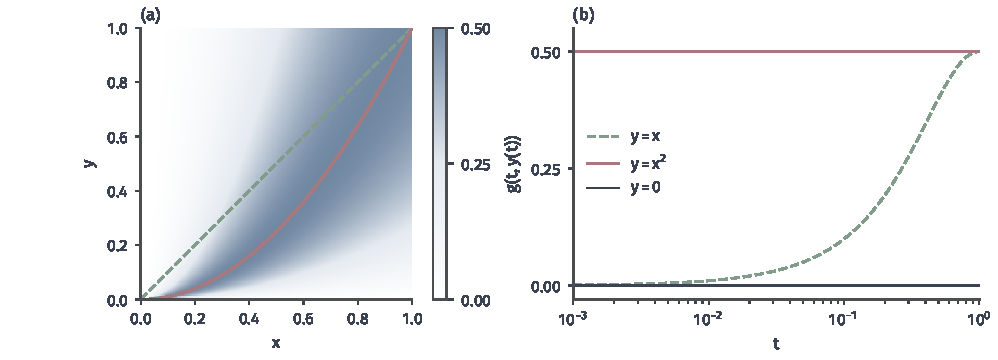
\includegraphics[width=169.0mm]{figures/00-shared/mathematical-preliminaries-upper/00-shared/matplotlib/chapter3-concept-processes/joint-limit-paths.pdf}
 \caption{取前例$g(x,y)=x^2y/(x^4+y^2)$，原点另置零。(a) 第一象限的函数值及三条路径，色阶固定为$0$至$1/2$。(b) 沿$y=0$、$y=x$分别趋零，沿$y=x^2$恒为$1/2$；横轴为正参数$t$的对数刻度，向左趋近原点。不同路径极限足以否定联合极限，有限条路径不能反向证明存在。}
 \label{fig:analysis-process-joint-limit-paths}
\end{figure*}

\paragraph{累次极限与联合极限}
另一种常见做法是逐个坐标取极限，即累次极限。它改变了问题的量词：先令$y\to0$、再令$x\to0$，考察的是
$\lim_{x\to0}\lim_{y\to0}f(x,y)$。内层固定$x\neq0$，让$y$单独趋于$0$；得到一个关于$x$的函数后，外层再让$x$趋于$0$。整个过程没有要求两个坐标同时趋近。
对示例~\ref{ex:multivariable-path-limits}中的$f$，固定$x\neq0$时$f(x,y)\to0$，再令$x\to0$仍为$0$；交换次序同样得到$0$。两个次序的累次极限都为$0$，联合极限却不存在。

累次极限的次序本身也会影响结果。
\begin{example}[两个次序的累次极限不相等]
\label{ex:multivariable-iterated-limits-differ}
在非原点处令$h(x,y)=x^2/(x^2+y^2)$。固定$x\neq0$而令$y\to0$，得到$x^2/x^2=1$；固定$y\neq0$而令$x\to0$，得到$0$。再取外层极限，
\[
 \begin{gathered}
\lim_{x\to0}\lim_{y\to0}h(x,y)=1\\
\lim_{y\to0}\lim_{x\to0}h(x,y)=0.
 \end{gathered}
\]
内层先把一个坐标压到零，相当于先走到某条坐标轴附近，再沿坐标轴靠近原点。$h$在$x$轴上恒为$1$、在$y$轴上恒为$0$，两种次序因而给出不同结果。
\end{example}

所以累次极限相等不是联合极限存在的充分条件，改变次序也可能改变累次极限。

反方向在补充条件下成立：若联合极限$\lim_{(x,y)\to(0,0)}f(x,y)=L$存在，并且对充分接近$0$的每个$x\neq0$，内层极限$\lim_{y\to0}f(x,y)$都存在，则累次极限$\lim_{x\to0}\lim_{y\to0}f(x,y)$也存在且等于$L$。理由是：给定$\varepsilon>0$，取联合极限定义中的$\delta$；当$0<|x|<\delta/2$、$0<|y|<\delta/2$时$|f(x,y)-L|<\varepsilon$，令$y\to0$，内层极限与$L$相差不超过$\varepsilon$。

\paragraph{统一误差估计}
要证明联合极限存在，可以寻找只依赖距离的上界：若$|f(\bm x)-L|$不超过一个只与$\lVert\bm x-\bm a\rVert_2$有关、并随距离趋于零的量，所有路径就同时受到控制。
\begin{example}[用距离上界证明联合极限]
\label{ex:multivariable-distance-bound-limit}
在非原点处考虑$x^2y/(x^2+y^2)$。由$|xy|\leq(x^2+y^2)/2$，有
\[
 \left|\frac{x^2y}{x^2+y^2}\right|
 =|x|\cdot\frac{|xy|}{x^2+y^2}
 \leq \frac{|x|}{2}
 \leq\frac12\sqrt{x^2+y^2}.
\]
给定$\varepsilon>0$，取$\delta=2\varepsilon$，则距离原点小于$\delta$的非原点都满足误差小于$\varepsilon$，因此原点处极限为$0$。

改用极坐标$(x,y)=(r\cos\theta,r\sin\theta)$，同一函数等于$r\cos^2\theta\sin\theta$，绝对值不超过$r$。这个界对所有$\theta$同时成立，给出同样的结论。
\end{example}

极坐标估计有效的关键是界与角度无关。若只固定$\theta$再令$r\to0$，检查的仍然只是直线。
\begin{example}[固定角度的极坐标检验]
\label{ex:multivariable-polar-fixed-angle}
对示例~\ref{ex:multivariable-parabola-path-limit}中的$g$，代入$(x,y)=(r\cos\theta,r\sin\theta)$得到
\[
 g=\frac{r\cos^2\theta\sin\theta}{r^2\cos^4\theta+\sin^2\theta}.
\]
固定$\theta$再令$r\to0$：$\sin\theta\neq0$时分母趋于$\sin^2\theta$而分子趋于$0$，$\sin\theta=0$时函数恒为$0$，结果总是$0$。
但对每个小的$r>0$，可以取满足$\sin\theta=r\cos^2\theta$的角度。此时分子等于$r^2\cos^4\theta$、分母等于$2r^2\cos^4\theta$，函数值恰为$1/2$。这个角度随$r$改变，对应的点$(r\cos\theta,r\sin\theta)$满足$y=r^2\cos^2\theta=x^2$，正好落在抛物线上。
\end{example}

因此用极坐标证明联合极限时，需要一个对全部$\theta$同时成立、并随$r\to0$趋于零的界。

\subsection{极限的运算与连续性}
\label{sec:multivariable-continuity}

连续性要求输入联合趋近基点时，输出趋于基点处的函数值。定义形式与一元连续性相同，只是把$|x-a|$换成欧氏距离；给出定义后，再检验和、差、数乘、积、商与复合是否保持连续性。
\begin{definition}[多元标量函数的连续性]
\label{def:multivariable-scalar-continuity}
设$f:D\subseteq\mathbb R^d\to\mathbb R$、$\bm a\in D$。若对每个$\varepsilon>0$都存在$\delta>0$，使
\[
 \bm x\in D,\quad\lVert\bm x-\bm a\rVert_2<\delta
 \Longrightarrow |f(\bm x)-f(\bm a)|<\varepsilon,
\]
则称$f$在$\bm a$处连续；在$D$上每点连续时称$f$为连续函数。
\end{definition}
在聚点处，这等价于联合极限等于$f(\bm a)$；在孤立点处，取足够小的$\delta$使球内只有$\bm a$，定义自动成立。
几何上，连续意味着曲面在$\bm a$上方没有裂缝或跳跃：从任何方向走近，高度都平稳地接近$f(\bm a)$。
固定其他输入坐标后的一元切片连续只是必要条件，示例~\ref{ex:multivariable-path-limits}说明它不足以保证联合连续。

\paragraph{和的连续性}
设$f,g$在$\bm a$处连续。由三角不等式，
\[
 |(f+g)(\bm x)-(f+g)(\bm a)|\leq|f(\bm x)-f(\bm a)|+|g(\bm x)-g(\bm a)|.
\]
给定$\varepsilon>0$，分别取使两个误差都小于$\varepsilon/2$的半径，其中较小的半径就满足$f+g$的连续性要求。

\paragraph{差的连续性}
相减时两项的误差仍按三角不等式相加：$|(f-g)(\bm x)-(f-g)(\bm a)|\leq|f(\bm x)-f(\bm a)|+|g(\bm x)-g(\bm a)|$。取与和相同的半径，即得$f-g$在$\bm a$处连续。

\paragraph{数乘的连续性}
对固定实数$c$，有$|cf(\bm x)-cf(\bm a)|=|c|\,|f(\bm x)-f(\bm a)|$。$c\neq0$时，把$f$的误差控制在$\varepsilon/|c|$以内即可；$c=0$时$cf$是常函数，结论直接成立。

\paragraph{积的连续性}
若$f,g$在$\bm a$处连续，乘积的误差可以拆成两项：
\[
 f(\bm x)g(\bm x)-f(\bm a)g(\bm a)
 =f(\bm x)\bigl(g(\bm x)-g(\bm a)\bigr)+g(\bm a)\bigl(f(\bm x)-f(\bm a)\bigr).
\]
由$f$的连续性，$\bm x$足够靠近$\bm a$时$|f(\bm x)|\leq|f(\bm a)|+1$，第一项的因子$f(\bm x)$有界；两个括号又都趋于零，所以$fg$在$\bm a$处连续。这与一元的乘积极限法则是同一个论证。

坐标函数$\bm x\mapsto x_j$连续，因为$|x_j-a_j|\leq\lVert\bm x-\bm a\rVert_2$。多元多项式由坐标函数和常数经有限次加法与乘法得到，因此连续，例如$x^2+xy+y^2$。

\paragraph{商的连续性}
除法还要防止分母变为零。若再设$g(\bm a)\neq0$，由$g$的连续性，可以取一个小球使其中$|g(\bm x)|>|g(\bm a)|/2$，即$g$在基点附近远离零。于是
\[
 \left|\frac1{g(\bm x)}-\frac1{g(\bm a)}\right|
 =\frac{|g(\bm x)-g(\bm a)|}{|g(\bm x)|\,|g(\bm a)|}
 \leq\frac{2|g(\bm x)-g(\bm a)|}{g(\bm a)^2}\longrightarrow0,
\]
所以$1/g$在$\bm a$处连续，再用积的连续性得到$f/g$连续。分母非零的条件不能省略，否则商在基点没有定义；由此，有理函数在分母非零处连续。

\paragraph{标量复合函数}
若$f:D\to\mathbb R$在$\bm a$处连续，一元函数$\psi$在$f(\bm a)$处连续，且$f$在$\bm a$附近的输出都在$\psi$的定义域内，则$\psi\circ f$在$\bm a$处连续。
证明分两步控制误差。给定$\varepsilon>0$，先由$\psi$的连续性取$\eta>0$，使中间实数与$f(\bm a)$相差小于$\eta$时，$\psi$的输出误差小于$\varepsilon$；再由$f$的连续性取$\delta>0$，使输入距离小于$\delta$时，$f$的输出与$f(\bm a)$相差小于$\eta$。合并两步，$\lVert\bm x-\bm a\rVert_2<\delta$时就有$|\psi(f(\bm x))-\psi(f(\bm a))|<\varepsilon$。
例如$e^{-(x^2+y^2)}$和$\sqrt{1+x^2+y^2}$都是一元连续函数与多项式的复合，因而在整个平面上连续。

\subsection{闭有界集上的连续函数}

寻找多元函数的最小值之前，先要知道最小值在什么条件下一定存在。机器学习中常在一块参数区域内最小化损失，如果最小值根本取不到，“求最小点”就没有对象。
一元情形中，闭区间上的连续函数一定取到最值，所用的关键事实是：闭区间内任意点列都有收敛于该区间内的子列。本小节先把这一子列性质推广到$\mathbb R^d$的闭有界集，再用它得到多元极值定理。

\paragraph{有限维闭有界集的收敛子列}
实数列的Bolzano--Weierstrass定理可以逐个坐标使用，得到多维输入所需的子列性质：有界性保证收敛子列存在，闭性保证极限点仍在集合内。
\begin{theorem}[有限维有界序列的收敛子列]
\label{thm:multivariable-bolzano-weierstrass}
若$(\bm x_n)$是$\mathbb R^d$中的有界序列，则存在严格递增的正整数序列$(n_k)$及$\bm a\in\mathbb R^d$，使$\bm x_{n_k}\to\bm a$。
若所有$\bm x_n$属于闭集$K$，则$\bm a\in K$。
\end{theorem}
\begin{proof}
序列有界，所以每个坐标组成的实数列也有界。以$d=2$为例：先用实数列定理，从第一坐标中选出收敛子列；在这个子列中，第二坐标仍是有界实数列，再从中选出收敛的子子列。子子列的第一坐标是收敛数列的子列，仍然收敛，因此两个坐标都收敛。一般的$d$重复这一步$d$次，每次都在上一步的子列中继续选取，最后全部坐标都收敛。
设各坐标极限组成$\bm a$，由$\lVert\bm x-\bm a\rVert_2\leq\sqrt d\max_j|x_j-a_j|$可知所得子列在欧氏距离下收敛于$\bm a$。
若所有项都属于闭集$K$，闭集包含其收敛序列的极限，故$\bm a\in K$。
\end{proof}
有限维闭有界集因此具有与闭区间相同的子列性质，极值定理的证明直接使用这一性质；一般度量空间中紧致与序列紧致的等价在\BookChapterRef{chap:metric-spaces}{第~\ref{chap:metric-spaces}章}讨论。

\paragraph{有界性与极值达到}
要保证上、下确界由定义域内的点取得，需要防止“函数值趋近确界的输入序列”逃出定义域：它可能跑向无穷远，也可能趋向一个不属于定义域的边界点。
闭有界集的子列性质同时排除了这两种情况。
\begin{theorem}[闭有界集上的极值定理]
\label{thm:multivariable-extreme-value}
设$K\subseteq\mathbb R^d$非空、闭且有界，$f:K\to\mathbb R$连续，则$f$有界，且存在$\bm x_{\min},\bm x_{\max}\in K$满足
\[
 f(\bm x_{\min})\leq f(\bm x)\leq f(\bm x_{\max})\qquad(\bm x\in K).
\]
\end{theorem}
\begin{proof}
定理~\ref{thm:analysis-extreme-value}的证明只用到两件事：定义域内任意点列有收敛于定义域内的子列，以及函数连续。
这里的$K$由定理~\ref{thm:multivariable-bolzano-weierstrass}满足同一子列条件，输出仍为实数，所以该证明逐字适用。例如对最大值，取$\bm x_n\in K$使$f(\bm x_n)$趋于上确界，选出收敛子列$\bm x_{n_k}\to\bm x_{\max}\in K$，连续性给出$f(\bm x_{\max})$等于上确界。
\end{proof}
定理的条件只是充分条件，但删去其中任何一个，结论都可能失败。与一元的示例~\ref{ex:analysis-extrema-failures}相同，可以逐项构造反例。
\begin{example}[删去闭性、有界性或连续性时最值可能取不到]
\label{ex:multivariable-extreme-value-failures}
在开单位圆盘$\{x^2+y^2<1\}$上，连续函数$f(x,y)=x^2+y^2$的上确界为$1$，但趋近上确界的点跑向不属于圆盘的边界圆，最大值取不到；这说明不能删去闭性。
在闭而无界的整个平面上，$f(x,y)=-(x^2+y^2)$在远处无限变小，没有下界；这说明不能删去有界性。
在闭单位圆盘上，令$f(x,y)=x^2+y^2$（$x^2+y^2<1$），并在边界圆上令$f=0$。定义域闭且有界，但$f$在边界圆上不连续，上确界$1$仍取不到；这说明不能删去连续性。
\end{example}

一元情形中讨论过的一致连续，换用欧氏距离后可以同样定义，闭有界集上的连续函数一致连续的结论也照样成立，本节不再展开。Lipschitz条件则在可微性之后结合中值定理讨论。

\section{多元标量函数的偏导数和梯度}

本节仍研究实值函数$f:U\subseteq\mathbb R^d\to\mathbb R$，并要求$U$为开集。开集中每一点都有一个含于$U$的小球，从基点出发向任何方向走足够小的一步仍在定义域内，双侧差商因而都有意义。
本节先计算坐标方向与一般方向上的变化率，再将各坐标偏导数排列为梯度，为下一节的局部线性近似作准备。

\subsection{偏导数与方向导数}

固定除$x_j$以外的全部坐标，$f$就变成只依赖$x_j$的一元函数，可以直接使用一元导数。
\begin{definition}[偏导数]
\label{def:multivariable-partial-derivative}
设$\bm a\in U$，令$\bm e_j$是第$j$个坐标为$1$、其余为$0$的向量。若双侧极限
\[
 \partial_jf(\bm a)=\frac{\partial f}{\partial x_j}(\bm a)
 =\lim_{t\to0}\frac{f(\bm a+t\bm e_j)-f(\bm a)}t
\]
存在且有限，就称它为$f$在$\bm a$处关于$x_j$的\term{偏导数}（partial derivative）。
\end{definition}
偏导数表示只改变第$j$个坐标、其余坐标固定时的变化率。符号$\partial$提醒我们：这里求的是多元函数的一个坐标切片的导数。
几何上，对二元函数，$\partial_xf(a,b)$是用竖直平面$y=b$截曲面所得曲线在$x=a$处的切线斜率；$\partial_yf(a,b)$则来自平面$x=a$的截线。把$f$看成平板上的温度，$\partial_xf$就是向正东方向移动时温度每单位距离的变化。

计算偏导数时，把其余坐标当作常数，按一元函数求导即可。
\begin{example}[二次函数的偏导数]
\label{ex:multivariable-quadratic-partials}
对$f(x,y)=x^2+xy+y^2$，把$y$当作常数对$x$求导，得到$f_x=2x+y$；把$x$当作常数对$y$求导，得到$f_y=x+2y$。
在$(1,2)$处，两者分别为$4$和$5$。直接用定义核对第一个值：
\[
 \frac{f(1+t,2)-f(1,2)}t=\frac{(1+t)^2+2(1+t)+4-7}{t}=4+t\longrightarrow4.
\]
再用数值核对：$f(1.01,2)=7.0401$，比$f(1,2)=7$大约$0.04=4\times0.01$；$f(1,2.01)=7.0501$，大约增加$5\times0.01$。
\end{example}

$f_x(1,2)=4$并不意味着朝任何方向走都以斜率$4$变化，每个偏导数只描述自己那条坐标切片。若同时走$(0.01,0.01)$，则$f(1.01,2.01)=7.0903$，增量约为$0.04+0.05$，像是两个偏导数贡献之和。这种“可以相加”并非总是成立，后面的可微性正是为它提供保证。

\paragraph{方向导数}

沿坐标轴求导只考察了$d$个方向。若让多个坐标按一个固定向量的比例共同移动，就得到另一条直线上的一元切片。
\begin{definition}[方向导数]
\label{def:multivariable-directional-derivative}
给定向量$\bm v\in\mathbb R^d$，若双侧极限
\[
 D_{\bm v}f(\bm a)
 =\lim_{t\to0}\frac{f(\bm a+t\bm v)-f(\bm a)}t
\]
存在且有限，就称它为沿$\bm v$的\term{方向导数}（directional derivative）。
\end{definition}
回到地形的比喻：站在$\bm a$上方，沿地图上的方向$\bm v$前进，方向导数就是脚下的坡度。
本书允许$\bm v$不是单位向量，这时导数按参数$t$的变化计量：$t$增加$1$，水平位置移动$\lVert\bm v\rVert_2$。若要表示每单位水平距离的变化率，应取$\lVert\bm v\rVert_2=1$。
取$\bm v=\bm e_j$便回到偏导数。双侧极限与只令$t\downarrow0$的单侧方向导数要分别判断。

方向向量的长度会改变方向导数的数值，比较同一条直线的两种参数化就能看清这一点。
\begin{example}[沿对角方向的方向导数]
\label{ex:multivariable-diagonal-directional-derivative}
仍取$f(x,y)=x^2+xy+y^2$，从$(1,2)$沿$\bm v=(1,1)^\top$移动，展开得
\[
 f(1+t,2+t)=(1+t)^2+(1+t)(2+t)+(2+t)^2=7+9t+3t^2,
\]
所以$D_{\bm v}f(1,2)=9$。
改用同向单位向量$\bm u=(1,1)^\top/\sqrt2$，参数$t$增加$1$时只走过单位距离，变化率为$D_{\bm u}f(1,2)=9/\sqrt2\approx6.36$。
\end{example}

两个方向向量描述同一条直线，但参数速度不同，比较变化率时不能忽略归一化约定。
还可以注意到$9=4\cdot1+5\cdot1$，恰好由两个坐标偏导数按方向分量组合得到。下一小节把坐标偏导数排列为梯度；随后，可微性将说明何时能用这样的组合求任意方向上的变化率。

\subsection{梯度的坐标表示}

各偏导数在同一基点计算，但分别对应不同输入坐标。将这些变化率按坐标顺序排成一列，就能用一个向量记录所有坐标切片的信息。
\begin{definition}[梯度]
\label{def:multivariable-gradient}
若$f:U\to\mathbb R$在$\bm a$处的各一阶偏导数都存在，称列向量
\[
 \nabla f(\bm a)=\bigl(\partial_1f(\bm a),\ldots,\partial_df(\bm a)\bigr)^\top
\]
为$f$在$\bm a$处的\term{梯度}（gradient）。
\end{definition}
由示例~\ref{ex:multivariable-quadratic-partials}，$f(x,y)=x^2+xy+y^2$的梯度为$\nabla f(x,y)=(2x+y,x+2y)^\top$，所以$\nabla f(1,2)=(4,5)^\top$。
梯度与输入属于同一个空间：$(4,5)^\top$可以画成地图平面上从$(1,2)$出发的一支箭头，而不是曲面上的向量。
就定义而言，梯度只是把各坐标的变化率并排放在一起。它能否预测所有坐标同时改变时的函数增量，箭头的方向又有什么含义，要等到第~\ref{sec:multivariable-total-differentiation}节的可微性才能回答。

\section{多元标量函数的可微性}
\label{sec:multivariable-total-differentiation}

偏导数和方向导数分别检查固定的坐标轴或直线。若要同时控制任意小扰动，包括方向不断改变的扰动，就需要一个对所有扰动共同有效的线性近似。

\subsection{全微分与可微性判别}

一元可微的含义是$f(a+h)=f(a)+f'(a)h+o(h)$：在$a$附近，函数图像可以用一条切线代替，误差比$h$小得多。把图像放大来看，曲线越来越像一条直线。
两个输入时，与切线对应的是切平面。把曲面$z=f(x,y)$在一点附近不断放大，如果它越来越像一张平面，就说$f$在该点可微，这张平面给出函数增量的最佳线性近似。

预测增量的规则应与扰动的叠加和数乘相容，因此使用线性映射$A:\mathbb R^d\to\mathbb R$。
例如$A(\bm h)=\bm c^\top\bm h$把每个坐标的扰动乘以固定系数再相加。可微性还要求遗漏的误差比扰动长度小得多。
\begin{definition}[多元标量函数的可微性与全微分]
\label{def:multivariable-total-differential}
设$U\subseteq\mathbb R^d$开，$f:U\to\mathbb R$，$\bm a\in U$。
若存在一个线性映射$A:\mathbb R^d\to\mathbb R$，使
\begin{equation}
\begin{gathered}
f(\bm a+\bm h)=f(\bm a)+A(\bm h)+o(\lVert\bm h\rVert_2)\\
\bm h\to\bm0,
\end{gathered}
\label{eq:analysis-total-differentiability}
\end{equation}
则称$f$在$\bm a$处\term{可微}（differentiable）。线性映射$A$称为该点的\term{全微分}（total differential），记为$\mathrm df_{\bm a}$。
\end{definition}
余项条件是$|f(\bm a+\bm h)-f(\bm a)-A(\bm h)|/\lVert\bm h\rVert_2\to0$，其中$\bm h\to\bm 0$按第~\ref{sec:multivariable-joint-limits}节的联合极限理解。
它要求同一个$A$适用于全部趋零扰动，而不是先固定一个方向、再让误差控制随方向改变。
$d=2$时，$z=f(\bm a)+A(\bm x-\bm a)$是三维空间中经过$(\bm a,f(\bm a))$的一张平面，即切平面；余项条件说的是，曲面与切平面的高度差比到$\bm a$的水平距离小得多。

这个“小得多”可以用数值观察。
\begin{example}[切平面误差随步长缩小]
\label{ex:multivariable-tangent-plane-error}
对$f(x,y)=x^2+xy+y^2$在$(1,2)$处，取线性映射$A(h,k)=4h+5k$（示例~\ref{ex:multivariable-quadratic-differential}将证明它就是全微分）。
取$(h,k)=(0.01,0.02)$，切平面预测$7+0.04+0.10=7.14$，实际值$f(1.01,2.02)=7.1407$，误差为$0.0007$，与步长$\sqrt{0.01^2+0.02^2}\approx0.0224$之比约为$0.031$。
把步长减半为$(0.005,0.01)$，误差变为$0.000175$，与步长$\approx0.0112$之比约为$0.016$，也减半。
\end{example}

误差与步长之比随步长减半而减半；步长继续缩小时，这个比值趋于零，这正是余项条件的要求。

\paragraph{可微性的要求与判别}
\label{sec:analysis-differentiability-relations}

本小节固定开集$U\subseteq\mathbb R^d$、标量函数$f:U\to\mathbb R$与基点$\bm a\in U$。
先说明统一线性近似必然满足哪些要求，并由此得到梯度的几何意义；再给出可核查的充分判别；最后用蕴含关系与反例区分偏导数存在、全部双侧方向导数存在、可微和连续可微。

\paragraph{可微的必要条件}
若同一个线性近似对全部扰动有效，把扰动限制在一条直线上，它就必须与这条直线上的一元导数相同；函数增量本身也必须趋于零。
这两点把全微分与偏导数、梯度及方向导数联系起来。
\begin{theorem}[可微性与梯度、方向导数]
\label{thm:multivariable-differentiable-necessary}
若$f:U\to\mathbb R$在$\bm a$处可微，则$f$在该点连续，各偏导数存在，并且
\[
 \begin{gathered}
\mathrm df_{\bm a}(\bm h)=\nabla f(\bm a)^\top\bm h\\
D_{\bm v}f(\bm a)=\nabla f(\bm a)^\top\bm v
 \quad(\bm v\in\mathbb R^d).
 \end{gathered}
\]
\end{theorem}
\begin{proof}
记$A=\mathrm df_{\bm a}$。先证连续。把$\bm h$按标准基写成$\sum_jh_j\bm e_j$，线性性给出$A(\bm h)=\sum_jh_jA(\bm e_j)$。由有限和的Cauchy--Schwarz不等式，
\[
 |A(\bm h)|\leq\left(\sum_j|A(\bm e_j)|^2\right)^{1/2}\lVert\bm h\rVert_2.
\]
因此在式~\eqref{eq:analysis-total-differentiability}中，线性项与余项都随$\bm h\to\bm 0$而趋零，即$f(\bm a+\bm h)\to f(\bm a)$，$f$连续。

再求系数。取$\bm h=t\bm e_j$，式~\eqref{eq:analysis-total-differentiability}变成$f(\bm a+t\bm e_j)-f(\bm a)=tA(\bm e_j)+o(|t|)$；两边除以$t$并令$t\to0$，可知偏导数存在且$\partial_jf(\bm a)=A(\bm e_j)$。代回线性展开，得到$A(\bm h)=\sum_j\partial_jf(\bm a)h_j=\nabla f(\bm a)^\top\bm h$。
最后对固定的$\bm v\neq\bm0$取$\bm h=t\bm v$：差商等于$\nabla f(\bm a)^\top\bm v$加上余项除以$t$，而余项是$o(|t|\lVert\bm v\rVert_2)$，除以$t$后仍趋零，就得到方向导数公式；$\bm v=\bm0$时差商恒为零。
\end{proof}
这个定理说明，一旦可微，全微分没有别的选择，只能是“梯度与扰动的内积”；所有方向导数也都由$d$个偏导数线性地决定。
因此验证可微时，候选线性映射已由梯度确定，只需再估计余项。对本节的二次函数，这一步可以直接完成。
\begin{example}[二元二次函数的全微分]
\label{ex:multivariable-quadratic-differential}
对二次函数$f(x,y)=x^2+xy+y^2$，在$(1,2)$处有$\nabla f=(4,5)^\top$。

设扰动为$(h,k)$，直接展开得
\[
 f(1+h,2+k)=7+4h+5k+(h^2+hk+k^2).
\]
由$|hk|\leq(h^2+k^2)/2$，最后一项绝对值不超过$3(h^2+k^2)/2$；除以$\sqrt{h^2+k^2}$后不超过$\tfrac32\sqrt{h^2+k^2}$，随扰动趋于零。所以全微分确为$\mathrm df_{(1,2)}(h,k)=4h+5k$，切平面为$z=7+4(x-1)+5(y-2)$。
\end{example}

这个全微分同时给出了示例~\ref{ex:multivariable-quadratic-partials}中的两个偏导数，以及示例~\ref{ex:multivariable-diagonal-directional-derivative}中沿$(1,1)^\top$的变化率$4+5=9$。
图~\ref{fig:analysis-process-total-differential-remainder}将这个全微分的切平面与统一余项界对应起来。
\begin{figure*}[!htbp]
 \centering
 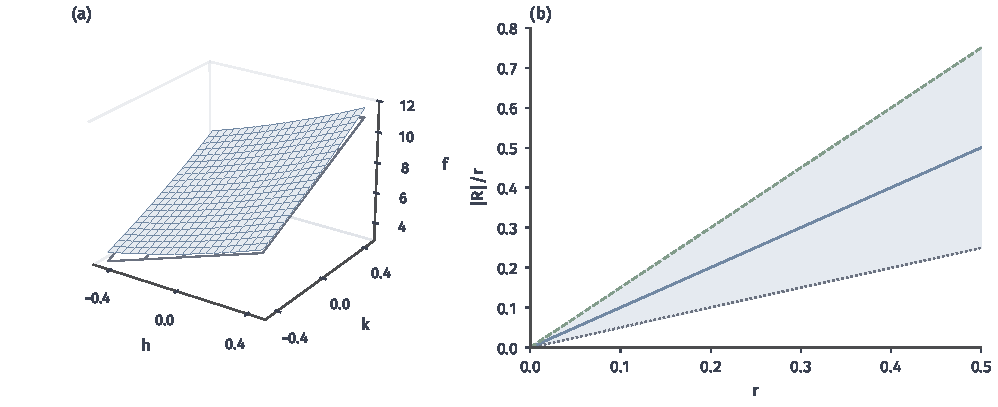
\includegraphics[width=169.0mm]{figures/00-shared/mathematical-preliminaries-upper/00-shared/matplotlib/chapter3-concept-processes/total-differential-remainder.pdf}
 \caption{(a) 二次函数在$(1,2)$附近，灰网格是切平面$P=7+4h+5k$，蓝面是$f(1+h,2+k)$。(b) 令$r=\sqrt{h^2+k^2}$，余项$R=h^2+hk+k^2$满足$r/2\leq R/r\leq3r/2$；阴影给出所有方向的完整范围，三条线是其中的代表值。共同上界随$r\to0$趋零，才保证任意方向都适用同一个线性近似。}
 \label{fig:analysis-process-total-differential-remainder}
\end{figure*}

\paragraph{偏导数连续给出的充分条件}
按定义验证可微，需要估计余项，通常不方便。另一种判别只检查偏导数：如果各坐标的变化率在基点附近连续变化，就可以沿坐标逐段走，用它们共同控制全部坐标增量。
与定理~\ref{thm:multivariable-differentiable-necessary}的必要条件不同，这项条件直接保证全微分存在。
\begin{theorem}[偏导数连续与可微性]
\label{thm:multivariable-continuous-partials-sufficient}
设$f:U\to\mathbb R$，$U$开，$\bm a\in U$。若各一阶偏导数在$\bm a$的某个邻域内存在，并在$\bm a$处连续，则$f$在$\bm a$处可微。
\end{theorem}
\begin{proof}
先看$d=2$。从$(a_1,a_2)$走到$(a_1+h_1,a_2+h_2)$，可以先竖直走、再水平走：
\[
 \begin{aligned}
 &f(a_1+h_1,a_2+h_2)-f(a_1,a_2)\\
 &=\bigl[f(a_1+h_1,a_2+h_2)-f(a_1,a_2+h_2)\bigr]\\
 &\quad+\bigl[f(a_1,a_2+h_2)-f(a_1,a_2)\bigr].
 \end{aligned}
\]
第一个方括号只改变第一个坐标，对一元函数$s\mapsto f(s,a_2+h_2)$用中值定理，得到它等于$\partial_1f(\bm\xi_1)h_1$，其中$\bm\xi_1$在这段水平线段上；第二个方括号同理等于$\partial_2f(\bm\xi_2)h_2$，$\bm\xi_2$在竖直线段上。这里用到$\bm h$足够小时两段都在偏导数存在的邻域内。

一般的$d$同样把$\bm a$到$\bm a+\bm h$的增量拆成$d$段，每段只改一个坐标，一元中值定理将第$j$段增量写成$\partial_jf(\bm\xi_j)h_j$，$\bm\xi_j$是第$j$段上的中间点。
减去候选线性项后，误差为$\sum_j\bigl(\partial_jf(\bm\xi_j)-\partial_jf(\bm a)\bigr)h_j$，因此
\[
 \begin{aligned}
 &\left|f(\bm a+\bm h)-f(\bm a)-\sum_{j=1}^d\partial_j f(\bm a)h_j\right|\\
 &\qquad\leq \max_j\left|\partial_j f(\bm\xi_j)-\partial_j f(\bm a)\right|
       \sum_{j=1}^d|h_j|
 =o(\lVert\bm h\rVert_2).
 \end{aligned}
\]
最后一步有两个依据：当$\bm h\to\bm0$时，所有中间点到$\bm a$的距离都不超过$\lVert\bm h\rVert_2$，偏导数在$\bm a$处连续，使最大值一项趋于零；另一方面$\sum_j|h_j|\leq\sqrt d\lVert\bm h\rVert_2$。
这样，各坐标方向上的变化就拼成了同一个有效的全微分。
\end{proof}
偏导数连续只是充分条件：可微仅要求函数增量具有统一的一阶近似，不要求这些系数随基点连续变化。实际计算中，若各偏导数在所论开集上由连续的表达式给出，例如多项式、分母非零的有理函数，以及它们与指数、正弦等连续函数的复合，就可以直接断定可微。

\paragraph{连续可微函数}
若还希望各点的一阶系数，即梯度，随基点连续变化，就需在一个范围内同时控制偏导数。
实值函数的各一阶偏导数在开集$U$上存在且连续时，称它在$U$上连续可微，记为$C^1(U)$；$C^k(U)$表示直至$k$阶的各偏导数都存在且连续。
定理~\ref{thm:multivariable-continuous-partials-sufficient}保证$C^1$函数处处可微，逆向并不成立，一元函数已经足以说明这一点。
\begin{example}[处处可微而导数无界]
\label{ex:multivariable-differentiable-not-c1}
在实轴上令$r(0)=0$，$x\neq0$时令$r(x)=x^2\sin(1/x^2)$。
由于$|r(h)/h|=|h\sin(1/h^2)|\leq|h|\to0$，有$r'(0)=0$；非零点按运算法则求导，得到
\[
 r'(x)=2x\sin(1/x^2)-\frac{2}{x}\cos(1/x^2).
\]
取$x_n=(2\pi n)^{-1/2}$，则$1/x_n^2=2\pi n$，$\sin$项为$0$、$\cos$项为$1$，于是$r'(x_n)=-2/x_n\to-\infty$。所以$r$处处可微，$r'$却在$0$附近无界，在$0$处不连续。
直观上，$r$的振幅被$x^2$压到零，图像在原点与横轴相切；但振荡越来越快，切线斜率剧烈摆动。
在多元情形令$f(\bm x)=r(x_1)$，就得到处处可微而非连续可微的标量函数。
\end{example}

这个例子还说明可微不保证局部Lipschitz连续：若$r$在原点的某个邻域内以$L$为Lipschitz常数，该邻域内每个差商的绝对值都不超过$L$，各点导数也就满足$|r'|\leq L$，与$r'(x_n)\to-\infty$矛盾。

\paragraph{条件之间的蕴含关系}
由必要条件与充分判别，可以把这些要求放在一起比较：
\[
 \begin{gathered}
 f\text{在}\bm a\text{的某邻域内连续可微}
 \ \Longrightarrow\ f\text{在}\bm a\text{处可微},\\
 f\text{在}\bm a\text{处可微}
 \ \Longrightarrow\ \text{全部双侧方向导数存在}
 \ \Longrightarrow\ \text{全部偏导数存在}.
 \end{gathered}
\]
第一条由定理~\ref{thm:multivariable-continuous-partials-sufficient}得到，第二条由定理~\ref{thm:multivariable-differentiable-necessary}得到，最后一条只须在全部方向中取坐标方向$\bm e_j$。
同一定理还说明，可微蕴含连续，并使方向导数关于方向成为同一个线性映射$\bm v\mapsto\nabla f(\bm a)^\top\bm v$。
第一行的前提涉及$\bm a$的整个邻域，其余条件只涉及基点$\bm a$本身；示例~\ref{ex:multivariable-differentiable-not-c1}已经说明，即使处处可微，也不能反推连续可微。

一元函数在一点的导数存在就等价于可微，因为实轴上只有一条直线可走。多元函数还须协调无穷多个输入方向以及弯曲的趋近路径，所以第二行的两个逆命题也不成立，以下依次给出反例。

\paragraph{偏导数存在不保证可微}
先看坐标偏导数：它们只约束两条坐标切片，并未控制其余方向或路径。
\begin{example}[偏导数存在但不可微]
\label{ex:analysis-partials-not-differentiable}
定义$f:\mathbb{R}^2\to\mathbb{R}$为
\[
 f(x,y)=
 \begin{cases}
  \dfrac{xy}{\sqrt{x^2+y^2}}, & (x,y)\neq(0,0),\\[6pt]
  0, & (x,y)=(0,0).
 \end{cases}
\]
沿两条坐标轴，函数恒为$0$，所以$\partial f/\partial x(0,0)=\partial f/\partial y(0,0)=0$。若$f$在原点可微，由定理~\ref{thm:multivariable-differentiable-necessary}，候选线性部分只能是零映射。可是沿$\bm{h}=(t,t)$，
\[
 \frac{|f(t,t)-f(0,0)|}{\lVert(t,t)\rVert_2}
 =\frac{|t|/\sqrt{2}}{\sqrt{2}|t|}
 =\frac12,
\]
余项与$\lVert\bm{h}\rVert_2$之比不趋于零，故$f$在原点不可微。

用极坐标可以看清曲面的形状：$f=r\cos\theta\sin\theta=\tfrac r2\sin2\theta$。沿每条从原点出发的射线，函数随$r$线性增长，斜率$\tfrac12\sin2\theta$随方向变化。曲面由这些射线组成，像一个起伏的锥面；把它放大任意倍数后形状不变，永远不会变得像一张平面。

沿每个方向$\bm v=(a,b)$，只令$t\downarrow0$的正向方向导数都存在，等于$ab/\sqrt{a^2+b^2}$（零方向取$0$），但它不是关于$\bm v$的线性函数。$t<0$时差商变号，因此$ab\neq0$时双侧方向导数不存在。
最后，由$|xy|/\sqrt{x^2+y^2}\leq\sqrt{x^2+y^2}/2$，$f$在原点连续。
\end{example}

偏导数只看坐标轴，遗漏了其他接近方向；可微则要求曲面放大后接近平面，本例的锥面做不到。这个例子还说明，偏导数存在、全部正向方向导数存在，再加上连续性，都不足以推出可微。方向极限采用单侧还是双侧，必须与所用定义一致；本节定义采用双侧极限。

\paragraph{全部方向导数存在不保证可微}
从坐标切片扩展到所有固定直线，仍需检查两件事：这些变化率能否组成一个线性映射，以及是否具有统一余项。先看缺少线性性的情形。
\begin{example}[方向导数不构成线性映射]
\label{ex:multivariable-nonlinear-directional-derivatives}
在非原点处令$p(x,y)=x^3/(x^2+y^2)$，并令$p(0,0)=0$。
沿$\bm v=(a,b)\neq\bm0$，差商为$p(ta,tb)/t=a^3/(a^2+b^2)$，不依赖$t$，所以双侧方向导数存在且$D_{\bm v}p(0,0)=a^3/(a^2+b^2)$。
取坐标方向得到候选梯度$(1,0)^\top$。若$p$可微，沿$(1,1)^\top$的方向导数应为$(1,0)(1,1)^\top=1$，实际却是$1/(1+1)=1/2$。这些方向变化率无法拼成一个线性映射，所以$p$在原点不可微。
\end{example}

与示例~\ref{ex:analysis-partials-not-differentiable}只有单侧方向极限不同，这里的双侧方向导数全部存在，失败只来自线性性。
即使方向导数全部存在并组成一个线性映射，仍需检查统一余项。
\begin{example}[方向导数全为零仍不可微]
\label{ex:multivariable-linear-directionals-not-differentiable}
在非原点处令$q(x,y)=x^3y/(x^4+y^2)$，并令$q(0,0)=0$。
由$2|x^2y|\leq x^4+y^2$，有$|q(x,y)|\leq|x|/2$，故$q$在原点连续。
对固定方向$(a,b)^\top$，若$b\neq0$，
\[
 \frac{q(ta,tb)}t=\frac{t a^3b}{t^2a^4+b^2}\longrightarrow0;
\]
若$b=0$，差商恒为零。因此所有双侧方向导数都为零，它们组成零线性映射。
可是沿$\bm h=(t,t^2)^\top$，$q(t,t^2)=t^5/(2t^4)=t/2$，从而
\[
 \frac{|q(t,t^2)|}{\lVert(t,t^2)\rVert_2}
 =\frac1{2\sqrt{1+t^2}}\longrightarrow\frac12.
\]
候选零映射不满足全微分的余项条件，$q$在原点不可微。
\end{example}

这与示例~\ref{ex:multivariable-parabola-path-limit}中$g$的情形相同：函数沿抛物线有一道坡，每条直线进入原点时都避开了它。方向导数先固定方向再取极限，全微分则要求对方向随扰动改变的序列也有同一个误差控制。

\paragraph{连续不保证偏导数存在}
反过来，连续性也推不出微分条件。
例如$f(x,y)=|x|$在整个平面上Lipschitz连续，图像沿$y$轴有一道折痕，原点关于$x$的双侧偏导数不存在，因此在那里不可微。
偏导数存在同样推不出连续：示例~\ref{ex:multivariable-path-limits}中原点置零的$xy/(x^2+y^2)$沿坐标轴恒为零，两个偏导数存在，但它在原点不连续。
因此连续与偏导数存在之间互不蕴含；可微则同时保证二者。

\paragraph{梯度与线性近似的使用条件}
上述反例区分了梯度的两种用途。仅有偏导数时，梯度只是坐标变化率排成的向量；确认可微以后，才可用它统一预测增量，用内积计算任意方向导数，并把它解释为最快上升的方向。
连续偏导数提供方便的充分判别，却不是必要条件；不满足该判别时，应回到全微分的统一余项定义检查。
讨论向量值函数时，同样对各个标量输出分量分别检查，再组成Jacobian矩阵及复合微分。

\subsection{微分的运算法则}

本小节的$f,g$都在同一开集内定义，并在基点$\bm a$处可微，$c$为固定实数。
各法则的证明方法相同：把各自的一阶展开代入，整理出关于$\bm h$的线性项，再确认剩下的部分仍是$o(\lVert\bm h\rVert_2)$。这样既得到新函数可微，也读出了它的全微分。

\paragraph{和的微分}
把两个一阶展开相加，
\[
 (f+g)(\bm a+\bm h)=(f+g)(\bm a)+\bigl(\mathrm df_{\bm a}+\mathrm dg_{\bm a}\bigr)(\bm h)+o(\lVert\bm h\rVert_2),
\]
两个线性映射之和仍是线性映射，两个$o(\lVert\bm h\rVert_2)$余项之和仍是$o(\lVert\bm h\rVert_2)$，因此
\[
 \begin{gathered}
\mathrm d(f+g)=\mathrm df+\mathrm dg\\
\nabla(f+g)=\nabla f+\nabla g.
 \end{gathered}
\]

\paragraph{差的微分}
把加号换成减号，同样的论证给出
\[
 \begin{gathered}
\mathrm d(f-g)=\mathrm df-\mathrm dg\\
\nabla(f-g)=\nabla f-\nabla g.
 \end{gathered}
\]

\paragraph{数乘的微分}
固定系数$c$只会缩放线性项与余项，故
\[
 \begin{gathered}
\mathrm d(cf)=c\,\mathrm df\\
\nabla(cf)=c\nabla f,
 \end{gathered}
\]
包括$c=0$的常函数情形。

\paragraph{积的微分}
记$R_f,R_g$为两个一阶展开的余项，都是$o(\lVert\bm h\rVert_2)$。相乘得
\[
 \begin{aligned}
 f(\bm a+\bm h)g(\bm a+\bm h)
 &=\bigl(f(\bm a)+\mathrm df(\bm h)+R_f\bigr)\bigl(g(\bm a)+\mathrm dg(\bm h)+R_g\bigr)\\
 &=f(\bm a)g(\bm a)+g(\bm a)\,\mathrm df(\bm h)+f(\bm a)\,\mathrm dg(\bm h)+(\text{其余各项}).
 \end{aligned}
\]
其余各项要么含有余项$R_f,R_g$乘以有界量，要么是两个线性增量的乘积$\mathrm df(\bm h)\,\mathrm dg(\bm h)=O(\lVert\bm h\rVert_2^2)$，都是$o(\lVert\bm h\rVert_2)$。因此乘积可微，且
\[
 \mathrm d(fg)=g(\bm a)\,\mathrm df+f(\bm a)\,\mathrm dg.
\]
这与一元的$(fg)'=f'g+fg'$形式相同：两个因子各自变化，一阶上贡献可以相加，两个变化同时发生的部分是高阶小量。

\paragraph{商的微分}
设$g(\bm a)\neq0$。可微蕴含连续，所以$g$在$\bm a$附近远离零，$1/g$在$\bm a$附近有定义。记$\delta=g(\bm a+\bm h)-g(\bm a)=\mathrm dg(\bm h)+o(\lVert\bm h\rVert_2)$，它是$O(\lVert\bm h\rVert_2)$。一元函数$1/y$在$g(\bm a)$处的展开给出
\[
 \frac1{g(\bm a)+\delta}=\frac1{g(\bm a)}-\frac{\delta}{g(\bm a)^2}+O(\delta^2).
\]
代入$\delta$的展开，并注意$O(\delta^2)=O(\lVert\bm h\rVert_2^2)$，得到$\mathrm d(1/g)=-\mathrm dg/g(\bm a)^2$。再把$f/g$看成$f\cdot(1/g)$，用积的微分得到
\[
 \mathrm d(f/g)=\frac{g(\bm a)\,\mathrm df-f(\bm a)\,\mathrm dg}{g(\bm a)^2}.
\]
这里分母非零既是定义商函数的条件，也是估计余项的条件。

\paragraph{标量复合函数的微分}
若一元函数$\psi$在$f(\bm a)$处可微，且复合在$\bm a$的邻域内有定义，则$\psi\circ f$在$\bm a$处可微，并且
\[
 \begin{gathered}
\mathrm d(\psi\circ f)=\psi'(f(\bm a))\,\mathrm df\\
\nabla(\psi\circ f)(\bm a)=\psi'(f(\bm a))\nabla f(\bm a).
 \end{gathered}
\]
推导时把内层增量$\delta=f(\bm a+\bm h)-f(\bm a)$代入外层的一元展开$\psi(f(\bm a)+\delta)=\psi(f(\bm a))+\psi'(f(\bm a))\delta+o(|\delta|)$，再把$\delta=\mathrm df(\bm h)+o(\lVert\bm h\rVert_2)$代入。
因为$\delta=O(\lVert\bm h\rVert_2)$，外层余项$o(|\delta|)$仍是$o(\lVert\bm h\rVert_2)$。
例如$\nabla e^{-(x^2+y^2)}=e^{-(x^2+y^2)}(-2x,-2y)^\top$：外层只把内层梯度乘上一个正数，所以复合函数的梯度与$-(x^2+y^2)$的梯度同向，都指向原点。

\paragraph{二次型的微分}
向量自变量的二次型仍是标量函数，机器学习中的平方误差、能量函数等都含有这种结构。考虑$q(\bm{x})=\bm{x}^{\top}\bm{A}\bm{x}=\sum_{i,j}A_{i,j}x_ix_j$，其中$\bm{A}\in\mathbb{R}^{d\times d}$固定。它是有限个乘积的和，乘积法则可以直接使用：把两个$\bm x$看成两个因子，每次只让一个变化，
\begin{align*}
  \mathrm{d}q
  &=
  (\mathrm{d}\bm{x})^{\top}\bm{A}\bm{x}
  +\bm{x}^{\top}\bm{A}\,\mathrm{d}\bm{x}\\
  &=
  \bm{x}^{\top}(\bm{A}^{\top}+\bm{A})\,\mathrm{d}\bm{x}.
\end{align*}
第二步用到$(\mathrm d\bm x)^\top\bm A\bm x$是一个实数，等于自己的转置$\bm x^\top\bm A^\top\mathrm d\bm x$。把$\mathrm dq$写成$\nabla q^\top\mathrm d\bm x$的形式，就读出
\begin{equation}
  \nabla_{\bm{x}}
  \bigl(\bm{x}^{\top}\bm{A}\bm{x}\bigr)
  =
  (\bm{A}+\bm{A}^{\top})\bm{x}.
\label{eq:analysis-quadratic-form-gradient}
\end{equation}
当$\bm{A}$对称时，式~\eqref{eq:analysis-quadratic-form-gradient}化为$2\bm{A}\bm{x}$，与一元的$(ax^2)'=2ax$对应；$\bm A$不对称时直接写成$2\bm{A}\bm{x}$，等于悄悄加入了对称性条件。
例如$\bm A=\begin{bmatrix}0&1\\0&0\end{bmatrix}$时$q=x_1x_2$，直接求偏导得$\nabla q=(x_2,x_1)^\top$，与$(\bm A+\bm A^\top)\bm x$一致；而$2\bm A\bm x=(2x_2,0)^\top$是错的。

\subsection{梯度的几何意义}

全微分是扰动上的线性泛函。指定内积以后，它有唯一的内积表示向量，这就是梯度；在非标准坐标中，要用Gram矩阵把坐标偏导换成该向量的坐标。

方向导数公式还说明了梯度指向哪里。

设$f$在$\bm a$处可微，对单位方向$\bm u$，由内积不等式，$D_{\bm u}f(\bm a)=\nabla f(\bm a)^\top\bm u\leq\lVert\nabla f(\bm a)\rVert_2$。
梯度非零时，取$\bm u=\nabla f(\bm a)/\lVert\nabla f(\bm a)\rVert_2$即达到等号，所以梯度方向是局部上升最快的单位方向。
这些结论都需要可微性，不能只由梯度向量存在推出。

图~\ref{fig:analysis-process-gradient-level-curves}用同一个二次函数比较梯度方向、等值曲线切向及另一个单位方向。
\begin{figure}[!htbp]
 \centering
 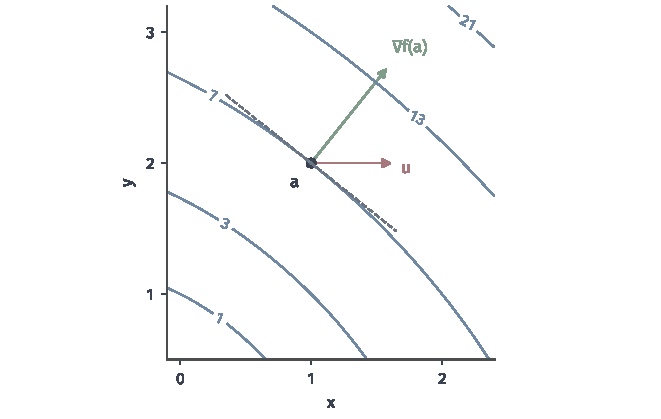
\includegraphics[width=112.0mm]{figures/00-shared/mathematical-preliminaries-upper/00-shared/matplotlib/chapter3-concept-processes/gradient-level-curves.pdf}
 \caption{$f=x^2+xy+y^2$的等值曲线，标注为函数值；基点$a=(1,2)$处$\nabla f=(4,5)^\top$，图中绿箭头按$0.15$倍绘制。灰虚线沿$(5,-4)^\top$，与梯度垂直，因而与经过$a$的等值曲线相切；红箭头为$u=(1,0)^\top$。比较最快上升方向时须先归一化，不能直接比较图中箭头长度。}
 \label{fig:analysis-process-gradient-level-curves}
\end{figure}

\subsection{中值估计与局部Lipschitz性}

导数控制一点处的变化；要估计两点之间的有限变化，可以沿连接两点的线段把函数限制为一元函数，再使用一元中值定理。前提是整条线段都在定义域内。
记$[\bm x,\bm y]=\{\bm x+t(\bm y-\bm x):0\leq t\leq1\}$为连接两点的线段。
\begin{theorem}[多元标量函数的中值公式]
\label{thm:multivariable-scalar-mean-value}
设$f$在包含$[\bm x,\bm y]$的开集上可微，$\bm x\neq\bm y$。则存在$\theta\in(0,1)$使
\[
 f(\bm y)-f(\bm x)=\nabla f(\bm x+\theta(\bm y-\bm x))^\top(\bm y-\bm x).
\]
\end{theorem}
\begin{proof}
令$\phi(t)=f(\bm x+t(\bm y-\bm x))$，$t\in[0,1]$，它是$f$在线段上的一元切片。$\phi'(t)$就是$f$在点$\bm x+t(\bm y-\bm x)$处沿$\bm y-\bm x$的方向导数，由定理~\ref{thm:multivariable-differentiable-necessary}，$\phi'(t)=\nabla f(\bm x+t(\bm y-\bm x))^\top(\bm y-\bm x)$。
对$\phi$在$[0,1]$上使用一元中值定理，$\phi(1)-\phi(0)=\phi'(\theta)$，这就是所述等式。
\end{proof}
等式说明，两点之间的平均变化率等于线段上某一点沿该方向的瞬时变化率，这是一元“平均斜率等于某点切线斜率”的直接推广。
例如$f(x,y)=x^2+y^2$，$\bm x=(0,0)$、$\bm y=(1,1)$，左侧为$2$；右侧为$\nabla f(\theta,\theta)^\top(1,1)^\top=4\theta$，取$\theta=1/2$即相等，中值点恰为线段中点。

\paragraph{局部Lipschitz性}

中值公式把有限增量写成某点梯度与位移的内积。若梯度的长度有统一上界，就能用输入距离的常数倍控制输出变化，这就是多元情形的Lipschitz条件。优化中常用它由步长控制函数值的变化。
\begin{definition}[多元函数的Lipschitz条件]
\label{def:multivariable-lipschitz}
设$D\subseteq\mathbb R^d$，$f:D\to\mathbb R$。若存在有限常数$L\geq0$，使
\[
 |f(\bm x)-f(\bm y)|\leq L\lVert\bm x-\bm y\rVert_2\qquad(\bm x,\bm y\in D),
\]
称$f$在$D$上Lipschitz连续，$L$称为Lipschitz常数。若每点都有一个邻域使$f$在其中Lipschitz连续（常数可随邻域改变），称$f$局部Lipschitz连续。
\end{definition}
这与一元定义只差把$|x-y|$换成欧氏距离。

例如线性函数$f(\bm x)=\bm a^\top\bm x$满足$|f(\bm x)-f(\bm y)|=|\bm a^\top(\bm x-\bm y)|\leq\lVert\bm a\rVert_2\lVert\bm x-\bm y\rVert_2$，Lipschitz常数可取$\lVert\bm a\rVert_2$。

欧氏范数$f(\bm x)=\lVert\bm x\rVert_2$由三角不等式满足$|\lVert\bm x\rVert_2-\lVert\bm y\rVert_2|\leq\lVert\bm x-\bm y\rVert_2$，常数为$1$，尽管它在原点不可微。

梯度界要转化为Lipschitz常数，还需要两点之间的线段留在定义域内。集合$D$称为凸集，是指其中任意两点之间的线段都含于$D$。在凸开集上，梯度长度的统一上界恰好就是Lipschitz常数。
\begin{theorem}[梯度有界与Lipschitz条件]
\label{thm:multivariable-gradient-lipschitz}
设$U\subseteq\mathbb R^d$为凸开集，$f:U\to\mathbb R$可微。则$f$在$U$上以$L$为Lipschitz常数，当且仅当$\lVert\nabla f(\bm x)\rVert_2\leq L$对所有$\bm x\in U$成立。
\end{theorem}
\begin{proof}
若梯度长度不超过$L$，任取$\bm x\neq\bm y$，凸性保证线段$[\bm x,\bm y]\subseteq U$。由中值公式与内积不等式，
\[
 |f(\bm y)-f(\bm x)|=\bigl|\nabla f(\bm\xi)^\top(\bm y-\bm x)\bigr|\leq\lVert\nabla f(\bm\xi)\rVert_2\lVert\bm y-\bm x\rVert_2\leq L\lVert\bm y-\bm x\rVert_2.
\]
反过来，设$f$以$L$为Lipschitz常数。固定$\bm x$，若$\nabla f(\bm x)\neq\bm0$，取单位方向$\bm u=\nabla f(\bm x)/\lVert\nabla f(\bm x)\rVert_2$，则
\[
 \lVert\nabla f(\bm x)\rVert_2=D_{\bm u}f(\bm x)=\lim_{t\downarrow0}\frac{f(\bm x+t\bm u)-f(\bm x)}t\leq\lim_{t\downarrow0}\frac{Lt}t=L.
\]
梯度为零时不等式自然成立。
\end{proof}
几何上，若坡度处处不超过$L$，沿直线走过距离$\rho$，高度最多改变$L\rho$；反过来，Lipschitz常数也限制了每一点最陡方向的坡度。
例如$f(x,y)=\sin x+\cos y$满足$\lVert\nabla f\rVert_2=\sqrt{\cos^2x+\sin^2y}\leq\sqrt2$，所以它在整个平面上以$\sqrt2$为Lipschitz常数。

定理中的凸性不能省略。在不凸的区域上，梯度可以处处很小，函数值却在两个很近的点之间相差很大。
\begin{example}[非凸区域上梯度有界而不Lipschitz]
\label{ex:multivariable-nonconvex-lipschitz-failure}
取去掉负$x$轴的环形区域$D=\{1<\lVert\bm x\rVert_2<2\}\setminus\{(x,0):x<0\}$，令$f(\bm x)$为点$\bm x$的极角，取值于$(-\pi,\pi)$。$f$在$D$上可微，$\lVert\nabla f\rVert_2=1/r<1$，坡度处处小于$1$。
但取负$x$轴两侧的点$(-1.5,\pm\varepsilon)$，两点距离为$2\varepsilon$，极角却分别接近$\pi$与$-\pi$，相差接近$2\pi$。令$\varepsilon\to0$，函数值之差与距离之比无界，所以$f$在$D$上不是Lipschitz函数。
\end{example}

连接这两点的直线段穿过被去掉的负$x$轴，不在$D$内，中值公式无法使用；$D$内连接两点的路径必须绕过原点，长度远大于$2\varepsilon$。梯度界只能沿含于定义域的线段转化为函数值之差的界。

局部情形同理。若$f\in C^1(U)$，在每个基点附近取一个包含在$U$内的闭球。连续函数$\lVert\nabla f\rVert_2$在这个闭有界集上有界（定理~\ref{thm:multivariable-extreme-value}），因而在同心的开球上也有界；开球是凸开集，故由定理~\ref{thm:multivariable-gradient-lipschitz}，$f$在这个开球上Lipschitz连续，从而局部Lipschitz连续。
局部常数不自动给出全域共同常数：$f(x,y)=x^2$连续可微，但$\lVert\nabla f\rVert_2=2|x|$在全平面无界，因而它不是全域Lipschitz函数。

\section{多元标量函数的高阶微分}
\label{sec:multivariable-curvature-error}

一阶微分用切平面描述局部变化，却看不出曲面向哪边弯：碗底、山顶和马鞍点处的切平面都是水平的。高阶微分记录一阶系数本身怎样变化，从而描述弯曲。
本节先把二阶偏导数集中为Hessian矩阵，再用Taylor公式建立二阶近似，最后据此判断驻点的局部极值类型。

\subsection{二阶偏导数、Hessian与高阶微分}

一阶偏导数本身仍是多元标量函数，可以再次求偏导。这里记$f_{x_i x_j}=\partial_j(\partial_i f)$，即先对$x_i$、再对$x_j$求导。
$f_{xx}$描述$x$方向切片的斜率沿$x$方向怎样变化，即该切片的弯曲；混合偏导数$f_{xy}$描述$x$方向的斜率在沿$y$方向移动时怎样变化，即曲面的扭转。

对$f(x,y)=x^2+xy+y^2$，有$f_{xx}=2$、$f_{xy}=f_{yx}=1$、$f_{yy}=2$。又如$f(x,y)=xy$，$x$方向切片的斜率是$y$，向北每走一单位，这个斜率就增加$1$，故$f_{xy}=1$，而$f_{xx}=f_{yy}=0$：每条坐标切片都是直线，曲面却是扭曲的。
这两个例子中$f_{xy}=f_{yx}$，但一般函数的混合偏导数能否交换次序，需要额外条件。

\paragraph{混合偏导数的交换}
分别沿两个坐标求导时，先后次序未必无关。
\begin{example}[混合偏导数与求导次序有关]
\label{ex:multivariable-mixed-partials-differ}
令$f(0,0)=0$，非原点处令
\[
 f(x,y)=\frac{xy(x^2-y^2)}{x^2+y^2}.
\]
对$y\neq0$，因为$f(0,y)=0$，
\[
 f_x(0,y)=\lim_{h\to0}\frac{f(h,y)}h=\lim_{h\to0}\frac{y(h^2-y^2)}{h^2+y^2}=-y;
\]
又$f$在$x$轴上恒为$0$，故$f_x(0,0)=0$，公式$f_x(0,y)=-y$在$y=0$时也成立。同样算得$f_y(x,0)=x$对所有$x$成立。于是
\[
 \begin{gathered}
f_{xy}(0,0)=\frac{\mathrm d}{\mathrm dy}(-y)\Big|_{y=0}=-1\\
f_{yx}(0,0)=\frac{\mathrm d}{\mathrm dx}x\Big|_{x=0}=1,
 \end{gathered}
\]
两个次序给出不同结果。
\end{example}

定理~\ref{thm:multivariable-mixed-partials}将说明，混合偏导数在基点连续时两种次序一定相同；因此本例的混合偏导数不可能都在原点连续。
\begin{theorem}[混合偏导数的交换]
\label{thm:multivariable-mixed-partials}
设$f$在$\bm a$的某个开邻域内有一阶偏导数$\partial_i f,\partial_j f$，混合偏导数$\partial_j\partial_i f,\partial_i\partial_j f$在该邻域存在并在$\bm a$处连续，则
\[
 \partial_j\partial_i f(\bm a)=\partial_i\partial_j f(\bm a).
\]
特别地，$C^2$函数的混合偏导数处处可以交换。
\end{theorem}
\begin{proof}
固定其他坐标，只需讨论二元函数在$(a,b)$处的情形。对小的非零$h,k$考察小矩形四个顶点上的二阶差分
\[
 \Delta(h,k)=f(a+h,b+k)-f(a+h,b)-f(a,b+k)+f(a,b).
\]
它可以按两种方式分组：先比较上下两边的差，或先比较左右两边的差，两种分组各给出一个混合偏导数。

令$\phi(x)=f(x,b+k)-f(x,b)$，则$\Delta=\phi(a+h)-\phi(a)$。先对$\phi$用一元中值定理，得到$\Delta=h\phi'(\xi)=h[f_x(\xi,b+k)-f_x(\xi,b)]$；再对$y\mapsto f_x(\xi,y)$使用一次中值定理，得到
\[
 \Delta=h[f_x(\xi,b+k)-f_x(\xi,b)]=hk f_{xy}(\xi,\eta),
\]
其中$\xi$在$a,a+h$之间、$\eta$在$b,b+k$之间。改用$\psi(y)=f(a+h,y)-f(a,y)$先沿$y$方向拆分，同样得到$\Delta=hk f_{yx}(\xi',\eta')$。
于是$f_{xy}(\xi,\eta)=f_{yx}(\xi',\eta')$。令$h,k\to0$，两个中间点都趋于$(a,b)$，连续性使两种混合偏导数在该点相等。
\end{proof}
示例~\ref{ex:multivariable-mixed-partials-differ}说明，只有混合偏导数存在而没有这些连续性条件时，结论可能失败。

\paragraph{Hessian矩阵}
把全部二阶偏导数排成一个方阵，就得到记录二阶信息的矩阵，它的行、列分别对应先后两次求导的输入坐标。
\begin{definition}[Hessian矩阵]
\label{def:multivariable-hessian}
若$f:U\to\mathbb R$在$\bm x$附近有一阶偏导数，且各$\partial_j\partial_i f(\bm x)$存在，则称
\[
 \nabla^2f(\bm x)=\bigl[\partial_j\partial_i f(\bm x)\bigr]_{i,j=1}^d
\]
为$f$在该点的\term{Hessian矩阵}（Hessian matrix）。
\end{definition}
第$i$行是第$i$个偏导数$\partial_if$的梯度（转置后），所以Hessian也可以理解为“梯度的梯度”：它说明当基点移动时，梯度向量怎样变化。
二阶偏导数存在本身尚不保证梯度映射$\nabla f$具有统一的线性近似；二阶可微要求$\nabla f$本身可微。
$C^2$是保证二阶可微的充分条件，且由定理~\ref{thm:multivariable-mixed-partials}，此时Hessian对称。对$x^2+xy+y^2$，Hessian就是$\begin{bmatrix}2&1\\1&2\end{bmatrix}$。

一元函数的二阶导数描述曲线向上还是向下弯；多元函数可以沿每个方向分别看。若$f\in C^2$，沿直线$t\mapsto f(\bm x+t\bm v)$求两次导数，在$t=0$处得到
\[
 \bm v^\top\nabla^2f(\bm x)\bm v
 =\sum_{i=1}^d\sum_{j=1}^d \partial_j\partial_i f(\bm x)v_i v_j.
\]
这一计算的依据在定理~\ref{thm:multivariable-second-order-taylor}的证明中给出。这个实数二次型衡量一阶斜率沿给定方向的变化，即沿方向$\bm v$截出的切片曲线的弯曲：为正时向上弯，为负时向下弯。

二次函数的Hessian可以直接读出。对
\[
 f(\bm{x})=\frac12\bm{x}^{\top}\bm{A}\bm{x}+\bm{b}^{\top}\bm{x}+c,
\]
只有$\bm{A}$的对称部分影响函数值，因为$\bm x^\top\bm A\bm x$与其转置$\bm x^\top\bm A^\top\bm x$相等。令$\bm{H}=(\bm{A}+\bm{A}^{\top})/2$，由式~\eqref{eq:analysis-quadratic-form-gradient}，$\nabla f(\bm{x})=\bm{H}\bm{x}+\bm{b}$，再求一次导得$\nabla^2f(\bm{x})=\bm{H}$。二次函数的Hessian是常数矩阵，各处弯曲相同。

例如$\bm H=\operatorname{diag}(2,100)$时，方向二次型为$2v_1^2+100v_2^2$：沿两个坐标方向都向上弯，但第二个方向的二阶变化率是第一个的$50$倍。函数图像是一个狭长的山谷：等值曲线是椭圆，沿$x_1$方向的半轴是沿$x_2$方向的$\sqrt{50}\approx7.1$倍。优化中这种形状会让梯度方法在陡峭方向来回摆动。
若改为$\operatorname{diag}(2,-100)$，两个坐标方向的弯曲方向便相反，图像是马鞍形。

这些情形按二次型的符号分类。第~\ref{sec:prelim-common-matrices}节已定义正定与半正定矩阵，这里把这些概念用于Hessian，并补充不定的情形：对实对称矩阵$\bm H$，若每个非零$\bm v$都有$\bm v^\top\bm H\bm v>0$，称$\bm H$正定；
若只要求$\bm v^\top\bm H\bm v\geq0$，则称半正定。
把不等号反向得到负定与半负定；若既存在使二次型为正的方向，又存在使它为负的方向，则称矩阵不定。
这些名称说明全部方向或某些方向上的曲率符号：正定对应各方向都向上弯的碗形，负定对应倒扣的碗，不定对应马鞍。

判断定性需要检查整个二次型，不能只看对角元素。
\begin{example}[用二次型判断Hessian的定性]
\label{ex:multivariable-hessian-definiteness}
对$\bm H=\begin{bmatrix}2&1\\1&2\end{bmatrix}$，配方得
\[
 \bm v^\top\bm H\bm v=2v_1^2+2v_1v_2+2v_2^2=(v_1+v_2)^2+v_1^2+v_2^2,
\]
非零$\bm v$时为正，所以$\bm H$正定。
对$\begin{bmatrix}1&2\\2&1\end{bmatrix}$，两个对角元都为正，但取$\bm v=(1,-1)^\top$得$1-4+1=-2<0$，取$\bm v=(1,1)^\top$得$6>0$，所以矩阵不定。
\end{example}

第二个矩阵的对角元只说明沿坐标轴向上弯；沿对角线$y=-x$，曲面却向下弯。

\paragraph{高阶微分的多线性形式}

Hessian不仅是一张二阶偏导数组，还规定了两个扰动方向之间的配对。

对$C^2$标量函数，记$H_f=\nabla^2f$，定义
\[
 D^2f_{\bm x}[\bm h,\bm k]=\bm h^\top H_f(\bm x)\bm k.
\]
它对两个方向分别线性，且由混合偏导相等而对称。二阶微分作用于两个不同方向，记录一个方向的变化率如何随另一个方向改变；把两个方向都取成$\bm h$，才得到Taylor公式中的二次项。

一般地，$f$为$C^r$时，令
\[
 D^rf_{\bm x}[\bm h_1,\ldots,\bm h_r]
 =\sum_{i_1,\ldots,i_r=1}^d
 \frac{\partial^rf}{\partial x_{i_1}\cdots\partial x_{i_r}}(\bm x)
 (h_1)_{i_1}\cdots(h_r)_{i_r}.
\]
有限和中的每一项对每个方向分别线性，所以这定义一个$r$重线性形式。连续混合偏导的交换使它对方向次序对称；坐标数组只是这个多线性作用在基下的记录。向量值微分建立后，也可以把它理解为对前一级微分再次求导。

例如$f(x,y)=x^2y$在$(1,2)$处的Hessian为$\left[\begin{smallmatrix}4&2\\2&0\end{smallmatrix}\right]$。方向$\bm h=(h_1,h_2)^\top$上的二次变化为$4h_1^2+4h_1h_2$；其中混合项说明两个坐标同时变化时，不能把两条坐标轴上的一元展开简单相加。

\subsection{多元Taylor展开与余项}

一元Taylor公式用导数构造多项式近似。把多个坐标同时改变的位移看成一条线段上的参数变化，就能沿这条线段使用一元Taylor公式。
所得公式针对标量输出：一次项给出切平面，二次项是一个实数二次型，补上曲面的弯曲。沿整条线段使用带Lagrange余项的一元公式，得到中间点形式的余项；再利用二阶偏导数在基点的连续性，得到小量形式的余项。
\begin{theorem}[多元标量函数的二阶Taylor公式]
\label{thm:multivariable-second-order-taylor}
设$f\in C^2(U)$，$U\subseteq\mathbb R^d$开，线段$[\bm x,\bm x+\bm h]\subset U$。若$\bm h\neq\bm 0$，则存在$\theta\in(0,1)$使
\begin{equation}
 f(\bm x+\bm h)=f(\bm x)+\nabla f(\bm x)^\top\bm h
 +\frac12\bm h^\top\nabla^2f(\bm x+\theta\bm h)\bm h.
\label{eq:analysis-second-order-taylor}
\end{equation}
对固定$\bm x\in U$，当$\bm h\to\bm 0$时还有
\begin{equation}
 f(\bm x+\bm h)=f(\bm x)+\nabla f(\bm x)^\top\bm h
 +\frac12\bm h^\top\nabla^2f(\bm x)\bm h+o(\lVert\bm h\rVert_2^2).
\label{eq:analysis-second-order-local-model}
\end{equation}
\end{theorem}
\begin{proof}
令$\phi(t)=f(\bm x+t\bm h)$。由定理~\ref{thm:multivariable-differentiable-necessary}的方向导数公式，$\phi'(t)=\nabla f(\bm x+t\bm h)^\top\bm h=\sum_i\partial_if(\bm x+t\bm h)h_i$。
每个$\partial_if$属于$C^1$，因而可微；对它再用一次方向导数公式，$\frac{\mathrm d}{\mathrm dt}\partial_if(\bm x+t\bm h)=\sum_j\partial_j\partial_if(\bm x+t\bm h)h_j$。相加得$\phi''(t)=\sum_{i,j}\partial_j\partial_if(\bm x+t\bm h)h_ih_j=\bm h^\top\nabla^2f(\bm x+t\bm h)\bm h$。
对$\phi$在$[0,1]$上使用带Lagrange余项的一元Taylor定理，$\phi(1)=\phi(0)+\phi'(0)+\tfrac12\phi''(\theta)$，即得第一式。

第二式要把中间点处的Hessian换成基点处的Hessian，并估计替换误差。$\theta\in(0,1)$可以随$\bm h$变化，但中间点$\bm x+\theta\bm h$到$\bm x$的距离不超过$\lVert\bm h\rVert_2$；Hessian各元素又在$\bm x$处连续，所以$\bm h\to\bm 0$时
$\lVert\nabla^2f(\bm x+\theta\bm h)-\nabla^2f(\bm x)\rVert_F\to0$。
对任意方阵$\bm B$，对$\sum_{i,j}B_{i,j}h_i h_j$使用有限和的Cauchy--Schwarz不等式，得到$|\bm h^\top\bm B\bm h|\leq\lVert\bm B\rVert_F\lVert\bm h\rVert_2^2$。取$\bm B$为两个Hessian之差，替换产生的误差不超过$\tfrac12\lVert\bm B\rVert_F\lVert\bm h\rVert_2^2=o(\lVert\bm h\rVert_2^2)$，得到第二式。
\end{proof}
用一个具体函数可以比较一阶近似与二阶近似的误差。
\begin{example}[指数函数的二阶Taylor近似]
\label{ex:multivariable-exponential-taylor}
令$f(x,y)=e^{x+y}$。在原点，函数值为$1$，梯度为$(1,1)^\top$，Hessian的各元素均为$1$，对应的二次型为$h^2+2hk+k^2=(h+k)^2$。由式~\eqref{eq:analysis-second-order-local-model}，
\[
 e^{h+k}=1+h+k+\frac12(h+k)^2+o(h^2+k^2).
\]
取$h=k=0.1$，实际值$e^{0.2}\approx1.22140$。切平面给出$1.2$，误差约$0.021$；加上二次项给出$1.22$，误差降到约$0.0014$。
\end{example}

一次项描述切平面，二次项补上沿位移方向的弯曲，所以加入二次项后误差明显减小。
式~\eqref{eq:analysis-second-order-local-model}则是局部结论。若要在一个区域内给出统一的余项界，还需在整个区域上控制Hessian的变化，例如假设Hessian满足Lipschitz条件；仅凭一点处的二阶导数不能得到这样的界。

若希望保留整条位移线段上的曲率，可以直接使用一元Taylor积分余项式~\eqref{eq:analysis-taylor-integral-remainder}。
在同一$C^2$条件下，令$\phi(t)=f(\bm x+t\bm h)$，取该式的$r=1$；把定理证明中算出的$\phi'$与$\phi''$代入，得到不挑选中间点的Taylor积分余项：
\[
 f(\bm{x}+\bm{h})
 =f(\bm{x})+\nabla f(\bm{x})^{\top}\bm{h}
 +\int_0^1(1-t)\,\bm{h}^{\top}\nabla^2f(\bm{x}+t\bm{h})\bm{h}\,\mathrm{d}t.
\]
权重$1-t$在起点$t=0$处最大、在终点处为零，所以越靠近位移起点的曲率对有限增量贡献越多。该表达式与式~\eqref{eq:analysis-second-order-taylor}描述同一有限变化，但不挑选中间点，而是保留整条线段上的曲率信息。

\subsection{驻点附近的函数形状}

Taylor公式把函数增量写成梯度项、Hessian二次型与高阶余项之和，因此梯度与Hessian的条件可以转化为原函数的极值结论。
先回顾极值的定义。若存在$\bm x^\star$的一个邻域，使其中定义域内的点的函数值都不小于$f(\bm x^\star)$，就称$\bm x^\star$为局部极小点；若邻域中其他点的函数值均严格更大，则称为严格局部极小点；局部极大点与严格局部极大点用反向不等式定义。
本小节只考察开集内部的点，不涉及约束。

\paragraph{局部极值的一阶必要条件}
一元函数在内部极值点处导数为零（Fermat条件）。把多元函数限制在任意一条过极值点的直线上，该点仍是所得一元函数的极值点，所以每个方向上的导数都必须为零。
几何上，这表示极值点处的切平面是水平的。
\begin{theorem}[局部极值的一阶必要条件]
\label{thm:multivariable-extremum-first-order}
设$f:U\to\mathbb R$在开集$U$内的点$\bm x^\star$处可微，且该点为局部极小点或局部极大点，则
\begin{equation}
 \nabla f(\bm x^\star)=\bm0.
\label{eq:analysis-first-order-necessary}
\end{equation}
\end{theorem}
\begin{proof}
对每个方向$\bm v$，一元函数$t\mapsto f(\bm x^\star+t\bm v)$在$0$处有局部极值，由Fermat条件和方向导数公式，导数$\nabla f(\bm x^\star)^\top\bm v=0$。
取各坐标方向$\bm v=\bm e_j$，即得全部偏导数为零。
\end{proof}
梯度为零的点称为驻点。驻点未必是极值点：$x^2-y^2$在原点梯度为零，但沿$x$轴原点是最低点，沿$y$轴却是最高点。要区分这些情形，需要二阶信息。

\paragraph{局部极值的二阶必要条件}
在极小点处，函数不能沿任何方向向下弯，否则沿该方向稍走一步，函数值就会变小。如果邻域内还具有连续二阶偏导数，这一要求就写成Hessian二次型的符号条件。
\begin{theorem}[局部极值的二阶必要条件]
\label{thm:multivariable-extremum-second-order}
设$f$在$\bm x^\star$附近属于$C^2$。若$\bm x^\star$为内部局部极小点，则
\begin{equation}
 \bm v^\top\nabla^2f(\bm x^\star)\bm v\geq0
 \qquad(\bm v\in\mathbb R^d),
\label{eq:analysis-second-order-necessary}
\end{equation}
即Hessian半正定；内部局部极大点对应Hessian半负定。
\end{theorem}
\begin{proof}
对每个$\bm v$，$\phi(t)=f(\bm x^\star+t\bm v)$在$0$处有局部极小，由一元极值的二阶必要条件，$\phi''(0)\geq0$；而定理~\ref{thm:multivariable-second-order-taylor}的证明已算出$\phi''(0)$正是所述二次型。
\end{proof}
必要条件不能单独决定驻点类型。一元函数$x^4$、$-x^4$及$x^3$在$0$处一阶、二阶导数都为零，却分别为极小、极大和非极值；多元函数在二次型为零的方向上同样要检查更高阶项。

\paragraph{驻点的二阶充分条件}
反过来，若各非零方向的二次型都严格为正，函数在驻点处沿所有方向都向上弯。Taylor余项是更高阶的小量，不会改变充分小扰动下函数增量的符号，于是驻点是严格极小点。正定比半正定更强：它要求每个方向都有正曲率，而不只是没有负曲率。
\begin{theorem}[驻点的Hessian判别]
\label{thm:multivariable-hessian-classification}
设$f$在$\bm x^\star$附近属于$C^2$，且$\nabla f(\bm x^\star)=\bm 0$。
若Hessian正定，则$\bm x^\star$是严格局部极小点；若负定，则为严格局部极大点；若不定，则任意小邻域都存在函数值大于及小于$f(\bm x^\star)$的点。
\end{theorem}
\begin{proof}
记$\bm H_\star=\nabla^2f(\bm{x}^{\star})$，先设它正定。
难点在于：每个方向的二次型为正，并不直接给出一个对所有方向共同的正下界，而余项估计需要这样的下界。
为此在闭有界的单位球面上考察连续函数$\bm v\mapsto\bm v^\top\bm H_\star\bm v$。
由定理~\ref{thm:multivariable-extreme-value}，它取到最小值
\[
 \lambda=\min_{\lVert\bm v\rVert_2=1}\bm v^\top\bm H_\star\bm v>0;
\]
最小值在某个单位向量处取得，正定性保证这个值为正。把任意非零$\bm h$写成$\lVert\bm h\rVert_2\bm v$，$\bm v$为单位向量，就得到
$\bm h^\top\bm H_\star\bm h\geq\lambda\lVert\bm h\rVert_2^2$。

再处理中间点处的Hessian。由Hessian矩阵的连续性，存在一个小球，使球内每点$\bm x$满足
$\lVert\nabla^2f(\bm x)-\bm H_\star\rVert_F\leq\lambda/2$。
对球内的非零$\bm h$，式~\eqref{eq:analysis-second-order-taylor}给出某个中间点$\bm\xi=\bm x^\star+\theta\bm h$，利用$\nabla f(\bm x^\star)=\bm 0$与Taylor公式证明中的不等式$|\bm h^\top\bm B\bm h|\leq\lVert\bm B\rVert_F\lVert\bm h\rVert_2^2$，
\[
 \begin{aligned}
 f(\bm{x}^{\star}+\bm{h})-f(\bm{x}^{\star})
 &=\frac12\bm h^\top\bm H_\star\bm h+\frac12\bm h^\top\bigl(\nabla^2f(\bm\xi)-\bm H_\star\bigr)\bm h\\
 &\geq\frac12\lambda\lVert\bm h\rVert_2^2-\frac12\cdot\frac{\lambda}{2}\lVert\bm h\rVert_2^2
 =\frac{\lambda}{4}\lVert\bm{h}\rVert_2^2>0,
 \end{aligned}
\]
故$\bm{x}^{\star}$是严格局部极小点。负定情形对$-f$使用同一论证，给出严格局部极大点。

若Hessian不定，分别选取使二次型为正和为负的方向$\bm v_+,\bm v_-$。
沿固定方向$\bm v$把扰动写成$t\bm v$，由式~\eqref{eq:analysis-second-order-local-model}，
\[
 f(\bm x^\star+t\bm v)-f(\bm x^\star)=\frac{t^2}{2}\bm v^\top\bm H_\star\bm v+o(t^2).
\]
充分小的非零$t$不会改变非零二次项的符号，因此沿$\bm v_+$函数值增加，沿$\bm v_-$函数值减小，任意小邻域内两种点都存在。
\end{proof}
不定情形中的驻点称为\term{鞍点}（saddle point），因为它像马鞍的中心：沿一个方向是最低点，沿另一个方向是最高点。
例如$f(x,y)=x^2-y^2$的Hessian为$\operatorname{diag}(2,-2)$，原点就是鞍点。

若Hessian矩阵仅半正定或半负定，且在某些非零方向上二次型为零，二阶判据可能没有结论，必须查看更高阶项或函数的其他结构。
上述必要条件还假定点位于开集内部。边界极小点的梯度可以不为零，例如$f(x)=x$在$[0,1]$上的最小点$0$；受约束问题需要\BookChapterRef{chap:constrained-optimization}{第~\ref{chap:constrained-optimization}章}的可行方向与乘子条件。

综合一阶与二阶条件，判别驻点分两步：先解$\nabla f=\bm 0$找出驻点，再在每个驻点检查Hessian的定性。
\begin{example}[驻点的分类]
\label{ex:multivariable-stationary-point-classification}
令$f(x,y)=x^3-3x+y^2$。梯度$\nabla f=(3x^2-3,\,2y)^\top$为零当且仅当$x=\pm1$、$y=0$，所以驻点是$(1,0)$与$(-1,0)$。
Hessian为$\operatorname{diag}(6x,2)$。在$(1,0)$处它是$\operatorname{diag}(6,2)$，正定，故$(1,0)$是严格局部极小点，$f(1,0)=-2$。在$(-1,0)$处它是$\operatorname{diag}(-6,2)$，不定，故$(-1,0)$是鞍点：沿$x$方向，$x^3-3x$在$-1$处取局部极大；沿$y$方向，$y^2$在$0$处取极小。
\end{example}

这个例子也说明局部极小不等于全局最小：沿负$x$轴$f\to-\infty$，该函数在整个平面上没有最小值。

图~\ref{fig:analysis-process-hessian-local-shapes}对照二阶判别可以决定的形状，以及Hessian退化时仍需继续检查的情形。
\begin{figure*}[!htbp]
 \centering
 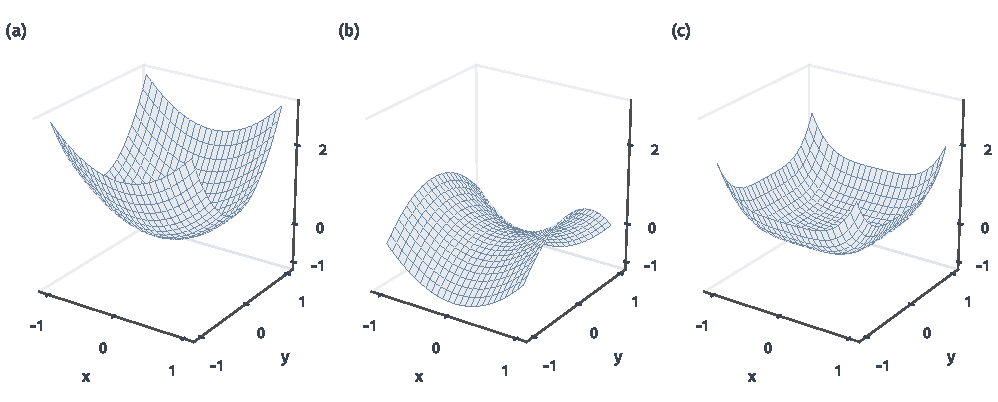
\includegraphics[width=169.0mm]{figures/00-shared/mathematical-preliminaries-upper/00-shared/matplotlib/chapter3-concept-processes/hessian-local-shapes.pdf}
 \caption{同一$[-1,1]^2$范围和纵轴尺度下，三面分别为$x^2+2y^2$、$x^2-y^2$、$x^4+y^4$。原点的Hessian依次为正定、不定、零矩阵；前两者给严格极小与鞍点，第三者虽严格极小却不能由正定判据推出。零Hessian也可能没有极值，例如前述$x^3$，故退化不是一种确定分类。}
 \label{fig:analysis-process-hessian-local-shapes}
\end{figure*}

\FloatBarrier

\section{多元向量值函数的微分}

前面每个输入只产生一个实数。现在固定$F:U\subseteq\mathbb R^d\to\mathbb R^m$，同一输入同时产生$m$个输出分量。例如极坐标映射$(r,\theta)\mapsto(r\cos\theta,r\sin\theta)$把两个参数变成平面上的点；神经网络的一层把输入向量变成另一个向量；参数曲线（$d=1$）与参数曲面（$d=2$、$m=3$）也是这种映射的特殊情况。
此时要问的是：输入稍作改变，输出点整体怎样移动。有限个输出可以逐分量检查，但每个分量的输入仍要整体扰动，不能以坐标切片代替各分量的全微分。

\subsection{向量值映射与Jacobian}

向量值函数由它的全部输出分量确定，因此按分量书写。
\begin{definition}[多元向量值函数]
\label{def:multivariable-vector-function}
映射$F:U\subseteq\mathbb R^d\to\mathbb R^m$称为多元向量值函数，写作$F=(F_1,\ldots,F_m)^\top$，其中每个$F_i:U\to\mathbb R$为多元标量函数。
\end{definition}
向量值函数的极限与连续性使用输出欧氏距离$\lVert F(\bm x)-\bm b\rVert_2$，即要求输出点整体接近$\bm b$。
对有限个输出，$F(\bm x)\to\bm b$等价于每个分量$F_i(\bm x)\to b_i$，$F$在一点连续也等价于每个$F_i$在该点连续，因为
\[
 \max_i|F_i(\bm x)-b_i|\leq\lVert F(\bm x)-\bm b\rVert_2
 \leq\sqrt m\max_i|F_i(\bm x)-b_i|.
\]
左侧不等式说明整体接近时每个分量都接近；右侧说明每个分量都接近到$\varepsilon/\sqrt m$以内时，整体误差小于$\varepsilon$。
这里分解的是输出分量，区别于只沿某些输入坐标检查的切片：每个分量$F_i$仍须在全部输入方向上联合趋近。

\paragraph{微分与Jacobian矩阵}

标量输出的全微分是到实数的线性映射，也称线性泛函；向量输出的全微分则要把输入扰动映射为$m$维输出扰动。
有限维线性映射由矩阵表示，矩阵的每一行记录一个输出分量的系数。
\begin{definition}[向量值函数的微分]
\label{def:multivariable-vector-differential}
设$U$开，$F:U\to\mathbb R^m$，$\bm a\in U$。若存在矩阵$\bm J_F(\bm a)\in\mathbb R^{m\times d}$，使
\begin{equation}
 F(\bm a+\bm h)=F(\bm a)+\bm J_F(\bm a)\bm h+o(\lVert\bm h\rVert_2),
\label{eq:analysis-jacobian-linearization}
\end{equation}
则称$F$在$\bm a$处可微，余项按输出欧氏范数理解。
其微分为$\mathrm dF_{\bm a}(\bm h)=\bm J_F(\bm a)\bm h$，其中$\bm J_F$称为\term{Jacobian矩阵}（Jacobian matrix），第$i,j$个元素为$\partial_jF_i$。
\end{definition}
向量值函数可微当且仅当每个输出分量$F_i$可微：正向可从向量余项取第$i$个分量，得到$F_i$的标量展开；反向则将有限个分量的$o(\lVert\bm h\rVert_2)$余项用欧氏范数合并，合并后仍是$o(\lVert\bm h\rVert_2)$。
因此Jacobian的第$i$行是标量分量梯度$\nabla F_i^\top$；$m=1$时Jacobian是梯度的转置，而不是梯度列向量本身。
$C^k$向量值函数指所有输出分量都属于$C^k$。

\paragraph{Jacobian矩阵的几何意义}
按列看Jacobian，第$j$列
\[
 \bm J_F(\bm a)\bm e_j=(\partial_jF_1,\ldots,\partial_jF_m)^\top
\]
表示：只把第$j$个输入增加一个很小的量$t$时，输出点大约沿这个向量移动$t$倍。一般扰动$\bm h=\sum_jh_j\bm e_j$的一阶效果就是这些列按$h_j$加权求和。
对$d=m=2$，这给出局部伸缩的图像：以$\bm a$为角、边长为$\varepsilon$的小正方形，由$\varepsilon\bm e_1,\varepsilon\bm e_2$张成，它的像近似是由$\varepsilon\bm J_F\bm e_1,\varepsilon\bm J_F\bm e_2$张成的平行四边形。行列式的绝对值是线性映射对面积的缩放倍数（第~\ref{sec:prelim-determinants}节），所以像的面积约为$|\det\bm J_F(\bm a)|\varepsilon^2$；行列式的符号说明局部是否翻转了定向。

极坐标映射给出这种局部伸缩的一个具体例子。
\begin{example}[极坐标映射的Jacobian矩阵]
\label{ex:multivariable-polar-jacobian}
考虑极坐标映射
\[
 P(r,\theta)=(r\cos\theta,r\sin\theta)^\top.
\]
逐个输出分量求偏导，得到
\[
\begin{gathered}
\bm J_P(r,\theta)=\begin{bmatrix}\cos\theta&-r\sin\theta\\ \sin\theta&r\cos\theta\end{bmatrix}\\
\det\bm J_P=r\cos^2\theta+r\sin^2\theta=r.
\end{gathered}
\]
第一列是单位径向向量：$r$增加$\mathrm dr$，点沿射线向外移动$\mathrm dr$。第二列长度为$r$、沿圆周切向：$\theta$增加$\mathrm d\theta$，点沿半径为$r$的圆移动约$r\,\mathrm d\theta$。因此参数平面中面积为$\mathrm dr\,\mathrm d\theta$的小矩形，变成面积约为$r\,\mathrm dr\,\mathrm d\theta$的小扇形块。
\end{example}

离原点越远，同样的角度增量扫过的弧越长，面积放大越多；第~\ref{sec:classical-change-variables}节的区域积分换元正是用这个倍数校正面积。

图~\ref{fig:analysis-process-jacobian-grid-cell}把一个非线性映射的线性近似画成小网格块的变化。图中$\det J_T(a)=1\times0.6-0.25\times0.3=0.525$，绿色小方块的像面积约为原面积的一半。
\begin{figure*}[!htbp]
 \centering
 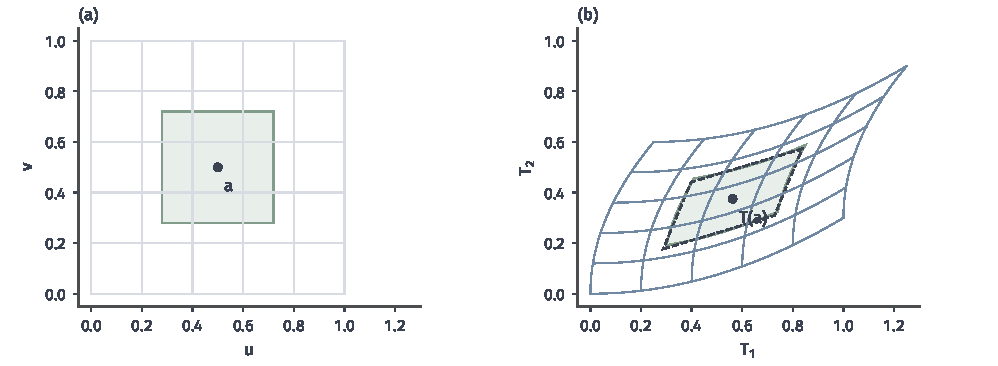
\includegraphics[width=169.0mm]{figures/00-shared/mathematical-preliminaries-upper/00-shared/matplotlib/chapter3-concept-processes/jacobian-grid-cell.pdf}
 \caption{取$T(u,v)=(u+v^2/4,\,0.6v+0.3u^2)$，$a=(0.5,0.5)$。(a) 输入网格及绿色小方块。(b) 非线性像为弯边块，黑虚线为$T(a)+J_T(a)(h,k)^\top$给出的平行四边形；$J_T(a)=\bigl[\begin{smallmatrix}1&0.25\\0.3&0.6\end{smallmatrix}\bigr]$。有限块不与线性像完全重合，缩小扰动后才由可微余项控制差异。}
 \label{fig:analysis-process-jacobian-grid-cell}
\end{figure*}

\paragraph{Jacobian矩阵的计算}
计算Jacobian矩阵时，每个输出先按标量函数求偏导，再按行排列；排好后可以核对输入、输出与矩阵形状是否一致。
例如$F(x,y)=(x^2+xy,y^2)^\top$的Jacobian为
\[
 \bm J_F(x,y)=\begin{bmatrix}2x+y&x\\0&2y\end{bmatrix}.
\]
在$(1,2)$处，它把扰动$(h,k)^\top$的一阶影响写成$(4h+k,4k)^\top$。两个输出分别占一行，两个输入分别占一列。

机器学习中一个常用的向量值映射，是把任意一组实数变成正数且总和为$1$的权重：先取指数，再除以共同的总和。
这就是$n$维\term{归一化指数映射}（softmax），分类模型常用它把各类别的得分变成概率。对正整数$n$和
$\bm{z}\in\mathbb{R}^n$，令
\[
 \begin{gathered}
s_i(\bm{z})
  =
  \frac{e^{z_i}}{\sum_{k=1}^n e^{z_k}}\\
i=1,\ldots,n.
 \end{gathered}
\]
记分母为$Z=\sum_k e^{z_k}$，它对$z_j$的偏导数为$e^{z_j}$。对分子$e^{z_i}$求偏导，$i=j$时得$e^{z_i}$，$i\neq j$时得$0$，记为$\mathbb{I}\{i=j\}e^{z_i}$。商法则给出
\[
  \frac{\partial s_i}{\partial z_j}
  =
  \frac{\mathbb{I}\{i=j\}e^{z_i}Z-e^{z_i}e^{z_j}}{Z^2}
  =
  s_i\bigl(\mathbb{I}\{i=j\}-s_j\bigr).
\]
因此整个Jacobian矩阵为
\begin{equation}
  \bm{J}_{\bm{s}}(\bm{z})
  =
  \operatorname{diag}(\bm{s})-\bm{s}\bm{s}^{\top}.
\label{eq:analysis-softmax-jacobian}
\end{equation}
这里$\operatorname{diag}(\bm s)$表示以$s_1,\ldots,s_n$为对角元、其他元素为零的对角矩阵。

当$n\geq2$时，对角项$s_i(1-s_i)$为正，描述提高$z_i$对自身分量的影响；非对角项$-s_is_j$为负，来自共同分母：提高一个得分会压低其余归一化分量。当$n=1$时输出恒为$1$，Jacobian为零。

每行元素之和为$s_i-s_i\sum_js_j=0$，这与给所有$z_i$同时加同一常数不改变输出相符：沿方向$(1,\ldots,1)^\top$的一阶变化为零。

在最简单的情形中，可以用数值核对式~\eqref{eq:analysis-softmax-jacobian}给出的线性近似。
\begin{example}[二维softmax的Jacobian矩阵]
\label{ex:multivariable-softmax-jacobian-check}
取$n=2$、$\bm z=\bm 0$，则$\bm s=(1/2,1/2)^\top$，由式~\eqref{eq:analysis-softmax-jacobian}，
\[
 \bm J_{\bm s}(\bm 0)
 =\begin{bmatrix}1/2&0\\0&1/2\end{bmatrix}-\begin{bmatrix}1/4&1/4\\1/4&1/4\end{bmatrix}
 =\begin{bmatrix}1/4&-1/4\\-1/4&1/4\end{bmatrix}.
\]
把$z_1$提高$0.1$，线性近似给出$\bm s$的增量约为
\[
 \bm J_{\bm s}(\bm 0)(0.1,0)^\top=(0.025,-0.025)^\top,
\]
即$s_1\approx0.525$、$s_2\approx0.475$。实际值为$s_1=e^{0.1}/(e^{0.1}+1)\approx0.52498$、$s_2\approx0.47502$。
\end{example}

线性近似与实际值只差约$2\times10^{-5}$，远小于输入改变量$0.1$；两个分量的增量一正一负、总和为零，与$s_1+s_2$恒为$1$相符。

\subsection{复合映射与导数的运算}
\label{sec:analysis-vector-chain-matrix-calculus}

运算法则以运算有定义为前提。输出形状相同的向量值函数可以相加、相减，任何向量值函数都可以数乘；复合则要求前一映射的输出落在后一映射的定义域内。
两个向量之间的乘法需要先指定含义（例如内积），本小节不讨论乘积法则。

\paragraph{和的微分}
若$F,H:U\to\mathbb R^m$在$\bm a$处可微，对每个输出分量分别使用标量的和法则，再把各分量的结果按行排回矩阵，得到
\[
 \bm J_{F+H}(\bm a)=\bm J_F(\bm a)+\bm J_H(\bm a).
\]
相加的输出形状以及两个Jacobian的形状必须分别一致。

\paragraph{差的微分}
在相同条件下，逐分量使用差法则，得到
\[
 \bm J_{F-H}(\bm a)=\bm J_F(\bm a)-\bm J_H(\bm a).
\]

\paragraph{数乘的微分}
对固定实数$c$，逐分量使用数乘法则，得到
\[
 \bm J_{cF}(\bm a)=c\bm J_F(\bm a).
\]

\paragraph{复合函数的链式法则}
复合映射$G\circ F$先用$F$把输入变成中间量，再用$G$把中间量变成输出。输入的小扰动$\bm h$先被$F$变成中间量的扰动，一阶上约为$\bm J_F\bm h$；这个扰动再被$G$变成输出扰动，一阶上约为$\bm J_G(\bm J_F\bm h)$。
因此复合微分按实际计算顺序组合，Jacobian的乘法次序由输入与输出维度决定。与一元情形一样，这项复合规则称为\term{链式法则}（chain rule）。
\begin{theorem}[向量值函数的链式法则]
\label{thm:multivariable-vector-chain-rule}
设$U\subseteq\mathbb R^d$、$V\subseteq\mathbb R^m$开，$F:U\to V$在$\bm a$处可微，$G:V\to\mathbb R^p$在$F(\bm a)$处可微，则$G\circ F$在$\bm a$处可微，且
\begin{equation}
 \bm J_{G\circ F}(\bm a)=\bm J_G(F(\bm a))\bm J_F(\bm a).
\label{eq:analysis-vector-chain-rule}
\end{equation}
\end{theorem}
\begin{proof}
记$\bm A=\bm J_F(\bm a)$、$\bm B=\bm J_G(F(\bm a))$。由$F$可微，中间量的增量为
\[
 \bm k=F(\bm a+\bm h)-F(\bm a)=\bm A\bm h+o(\lVert\bm h\rVert_2),
\]
故$\lVert\bm k\rVert_2\leq\lVert\bm A\bm h\rVert_2+o(\lVert\bm h\rVert_2)=O(\lVert\bm h\rVert_2)$：中间量的扰动与原扰动同阶。
代入$G$的一阶展开，
\[
 G(F(\bm a)+\bm k)-G(F(\bm a))=\bm B\bm k+o(\lVert\bm k\rVert_2)
 =\bm B\bm A\bm h+\bm B\,o(\lVert\bm h\rVert_2)+o(\lVert\bm k\rVert_2).
\]
右侧第二项中，矩阵$\bm B$至多把长度放大固定倍数，所以仍是$o(\lVert\bm h\rVert_2)$；第三项因$\lVert\bm k\rVert_2=O(\lVert\bm h\rVert_2)$也是$o(\lVert\bm h\rVert_2)$（$\bm k=\bm0$时外层余项为零）。
于是复合增量等于$\bm B\bm A\bm h$加上$o(\lVert\bm h\rVert_2)$，这正是复合函数的可微定义。
\end{proof}
式~\eqref{eq:analysis-vector-chain-rule}中的矩阵形状为$(p\times m)(m\times d)=p\times d$，反向相乘往往没有定义。
即使两个次序都有定义，矩阵乘法一般也不交换，不能按标量经验调换因子。
用局部伸缩的语言说：复合映射在一点附近的伸缩，等于两步伸缩依次作用；方阵情形下，行列式的乘法公式还给出面积缩放倍数相乘。

链式法则常用于这样的情形：先用向量值映射得到中间量，再把中间量变成一个标量，最后求这个标量对原输入的梯度。
\begin{example}[从中间向量求回复合目标的梯度]
\label{ex:analysis-chain-rule-calculation}
令
\[
 \begin{gathered}
F(x_1,x_2)=(x_1^2,x_1x_2,x_2)^\top\\
\ell(\bm y)=\frac12(y_1^2+y_2^2+y_3^2).
 \end{gathered}
\]
$F$从二维输入产生三维中间量，$\ell$再把三维中间量变成一个数，复合得到$L=\ell\circ F:\mathbb R^2\to\mathbb R$。
$\ell$的Jacobian是$1\times3$行向量$\nabla\ell(\bm y)^\top$，由链式法则，$L$的Jacobian为$\nabla\ell(F(\bm x))^\top\bm J_F(\bm x)$；转置后得到列向量梯度
\[
  \nabla L(\bm x)=\bm J_F(\bm x)^\top\nabla\ell\bigl(F(\bm x)\bigr).
\]
这里出现转置，是因为梯度按列向量书写，而链式法则中的$\ell$导数是行向量。本例中
\[
\begin{gathered}
\bm J_F=\begin{bmatrix}2x_1&0\\x_2&x_1\\0&1\end{bmatrix}\\
\nabla\ell(\bm y)=\bm y.
\end{gathered}
\]
在$\bm x=(1,2)^\top$处，$\bm y=(1,2,2)^\top$，链式法则给出
\[
  \nabla L(1,2)
  =\begin{bmatrix}2&2&0\\0&1&1\end{bmatrix}
    \begin{bmatrix}1\\2\\2\end{bmatrix}
  =\begin{bmatrix}6\\4\end{bmatrix}.
\]
也可以把复合函数直接展开为
$L(x_1,x_2)=\tfrac12(x_1^4+x_1^2x_2^2+x_2^2)$，求偏导得到
$\nabla L=(2x_1^3+x_1x_2^2,\,x_1^2x_2+x_2)^\top$，在同一点仍为$(6,4)^\top$。
矩阵形状$(2\times3)(3\times1)=2\times1$也核对了梯度传递的次序。
\end{example}

两种计算处理同一个目标；链式形式保留了中间映射，可以分别复用各层的导数。

\subsection{向量增量与导数范数估计}

标量函数的中值公式在线段上找到一个点，用那里的梯度精确表示增量。向量值函数不能照搬：各输出分量的一元中值点可能不同，没有一个共同位置代表整个向量增量。
例如$F(t)=(\cos t,\sin t)^\top$在$[0,2\pi]$上走完一整圈，$F(2\pi)-F(0)=\bm 0$，但速度$F'(t)=(-\sin t,\cos t)^\top$长度恒为$1$，不存在$\tau$使$F(2\pi)-F(0)=2\pi F'(\tau)$。
因此改为只控制增量的长度：用线性映射的最大放大倍数估计有限变化。

\paragraph{算子范数}

对标量函数，导数的绝对值说明输入的小变化被放大多少倍。对向量输出，同一矩阵在不同方向上放大的倍数可能不同，取其中最大的一个代替绝对值。
\begin{definition}[欧氏诱导算子范数]
\label{def:analysis-induced-operator-norm}
对矩阵
$\bm{A}\in\mathbb{R}^{s\times r}$，由欧氏范数\term{诱导的算子范数}
（induced operator norm）定义为
\[
  \lVert\bm{A}\rVert_{\mathrm{op}}
  =
  \sup_{\bm{h}\neq\bm{0}}
  \frac{\lVert\bm{A}\bm{h}\rVert_2}{\lVert\bm{h}\rVert_2}
  =
  \sup_{\lVert\bm{h}\rVert_2=1}\lVert\bm{A}\bm{h}\rVert_2.
\]
\end{definition}
算子范数是线性映射对向量长度的最大放大倍数，定义立即给出
$\lVert\bm{A}\bm{h}\rVert_2
\leq\lVert\bm{A}\rVert_{\mathrm{op}}\lVert\bm{h}\rVert_2$。
计算算子范数时，先给出对全部单位向量成立的上界，再找出达到上界的方向。
\begin{example}[对角矩阵的算子范数]
\label{ex:multivariable-diagonal-operator-norm}
令$\bm A=\operatorname{diag}(2,1)$，它把第一坐标放大两倍、第二坐标保持不变。对单位向量$\bm h$，
\[
 \lVert\bm A\bm h\rVert_2^2=4h_1^2+h_2^2\leq4(h_1^2+h_2^2)=4,
\]
且$\bm h=\bm e_1$时取等号，故$\lVert\bm A\rVert_{\mathrm{op}}=2$。
\end{example}

示例~\ref{ex:multivariable-diagonal-operator-norm}的最大放大由第一坐标方向达到。旋转矩阵不改变任何向量的长度，算子范数为$1$。

用算子范数控制增量长度后，就不再需要各分量共用一个中值点；所需条件是$G$在含整条线段的开集上连续可微。
\begin{theorem}[向量值函数的中值估计]
\label{thm:multivariable-vector-mean-value}
设$U\subseteq\mathbb R^r$开，$G:U\to\mathbb R^s$连续可微，且$[\bm y',\bm y]\subset U$，则
\begin{equation}
  \begin{aligned}
  \lVert G(\bm{y})-G(\bm{y}')\rVert_2
  &\leq
  \sup_{0\leq t\leq1}
  \left\lVert
    \bm{D}G\bigl(\bm{y}'+t(\bm{y}-\bm{y}')\bigr)
  \right\rVert_{\mathrm{op}}
  \lVert\bm{y}-\bm{y}'\rVert_2.
  \end{aligned}
\label{eq:analysis-operator-mean-value-bound}
\end{equation}
其中$\bm DG=\bm J_G$，即$G$的Jacobian矩阵。
\end{theorem}
\begin{proof}
思路是把向量增量投影到它自己的方向上，变成一个标量函数的增量，再对标量函数用中值定理。若$\bm u=G(\bm y)-G(\bm y')\neq\bm0$，
取单位向量$\bm v=\bm u/\lVert\bm u\rVert_2$，并沿线段定义标量函数
$\phi(t)=\bm v^\top G(\bm y'+t(\bm y-\bm y'))$。
由链式法则，$\phi'(t)=\bm v^\top\bm DG(\bm y'+t(\bm y-\bm y'))(\bm y-\bm y')$；中值定理给出某个$\tau\in(0,1)$，使
\[
 \lVert\bm u\rVert_2
 =\bm v^\top\bm u
 =\phi(1)-\phi(0)
 =\bm v^\top\bm DG(\bm y'+\tau(\bm y-\bm y'))(\bm y-\bm y').
\]
对右侧先用内积不等式并注意$\lVert\bm v\rVert_2=1$，再用算子范数的上界，便得到式~\eqref{eq:analysis-operator-mean-value-bound}；
$\bm u=\bm0$时该界直接成立。
\end{proof}
若定义域为凸开集，且Jacobian的算子范数在全域不超过同一个有限常数$L$，则由式~\eqref{eq:analysis-operator-mean-value-bound}，$G$以$L$为Lipschitz常数：任意两点的像之间的距离至多是原距离的$L$倍。在局部球上使用同样的界，就得到局部版本。
特别地，若Jacobian的算子范数在某个球内不超过一个常数$L<1$，映射就在球内严格缩小任意两点间的距离，称为压缩。第~\ref{sec:analysis-implicit-parameter-integral}节证明隐函数定理时，将用这一条件和几何级数的尾和控制迭代。

\section{矩阵函数的微分}

本小节的定义域$\mathcal U$均为全矩阵空间$\mathbb R^{m\times n}$中的开集，基点$\bm X\in\mathcal U$；因此全部充分小的同形扰动都允许使用。
机器学习中的参数常排成矩阵，例如线性层的权重或协方差矩阵，损失是它们的标量函数，求逆、相乘等运算又产生矩阵输出。原则上可以把矩阵拉直成长向量，再用前面的结论；但保留矩阵形状，能让乘法次序与迹的结构更清楚，结果也能直接写成矩阵表达式。

$m\times n$矩阵输入可以看成$mn$个实数坐标，$r\times s$矩阵输出可以看成$rs$个实数分量，因此可微性仍是“扰动的一阶变化由线性映射给出”；只是扰动用Frobenius范数度量，线性映射的输入与输出都保留矩阵形状。
第~\ref{sec:prelim-matrix-trace}节已定义Frobenius内积与范数，满足$\langle\bm A,\bm B\rangle_F=\operatorname{tr}(\bm A^\top\bm B)=\sum_{i,j}A_{i,j}B_{i,j}$，即把两个矩阵对应元素相乘再求和，也就是拉直后的向量内积。

\subsection{矩阵空间中的微分与梯度}
设$\Phi:\mathcal U\to\mathbb R^{r\times s}$。若存在矩阵空间之间的线性映射$\mathrm d\Phi_{\bm X}:\mathbb R^{m\times n}\to\mathbb R^{r\times s}$，使
\[
 \Phi(\bm X+\bm H)=\Phi(\bm X)+\mathrm d\Phi_{\bm X}(\bm H)+o(\lVert\bm H\rVert_F),
\]
余项按输出的Frobenius范数度量，则称$\Phi$在$\bm X$处可微，$\mathrm d\Phi_{\bm X}$为其微分。这就是向量值可微性按矩阵形状重排后的写法：Frobenius范数正是拉直后向量的欧氏范数。

计算时常写$\mathrm d\Phi=\mathrm d\Phi_{\bm X}(\mathrm d\bm X)$，用乘积法则展开后保留乘法次序。例如$\mathrm d(\bm A\bm X\bm B)=\bm A(\mathrm d\bm X)\bm B$，扰动夹在中间的位置不能移动。
又如$\Phi(\bm X)=\bm X^2=\bm X\bm X$，展开得$(\bm X+\bm H)(\bm X+\bm H)=\bm X^2+\bm H\bm X+\bm X\bm H+\bm H^2$。其中$\lVert\bm H^2\rVert_F\leq\lVert\bm H\rVert_F^2$是高阶项，故$\mathrm d(\bm X^2)=(\mathrm d\bm X)\bm X+\bm X(\mathrm d\bm X)$；只有$\bm X$与扰动交换时，才能写成$2\bm X\,\mathrm d\bm X$。

\paragraph{标量输出与矩阵梯度}
输出为标量（$r=s=1$）时，线性映射$\mathrm df_{\bm X}$可以用一个同形矩阵与扰动的Frobenius内积表示，这个矩阵就是梯度。这与向量情形$\mathrm df=\nabla f^\top\mathrm d\bm x$完全对应。
\begin{definition}[矩阵标量函数的梯度]
\label{def:multivariable-matrix-scalar-gradient}
设$f:\mathcal U\to\mathbb R$在$\bm X$处可微。唯一满足
\begin{equation}
 \mathrm df_{\bm X}(\bm H)=\langle\nabla_{\bm X}f,\bm H\rangle_F
 =\operatorname{tr}\bigl((\nabla_{\bm X}f)^\top\bm H\bigr)
\label{eq:analysis-matrix-gradient-definition}
\end{equation}
的同形矩阵$\nabla_{\bm X}f\in\mathbb R^{m\times n}$称为矩阵梯度。
\end{definition}
取只有第$(i,j)$个元素为$1$的扰动$\bm H$，右侧内积只剩$\nabla_{\bm X}f$的第$(i,j)$个元素，左侧是对$X_{i,j}$的偏导数。所以矩阵梯度的各元素就是对相应矩阵坐标的偏导数，唯一性也由此得到。与向量梯度一样，$\nabla_{\bm X}f$指出使$f$增加最快的扰动方向。

求梯度时，先用乘积法则展开微分，再利用迹的循环移位把扰动移到末端，写成$\operatorname{tr}(\bm G^\top\mathrm d\bm X)$的形式，便读出$\nabla_{\bm X}f=\bm G$。乘积形状相容时，
\[
 \begin{gathered}
\operatorname{tr}(\bm A\bm B)=\operatorname{tr}(\bm B\bm A)\\
\operatorname{tr}(\bm A\bm B\bm C)=\operatorname{tr}(\bm B\bm C\bm A).
 \end{gathered}
\]
这里循环移动的是整个因子，不能任意交换相邻矩阵。标量等于自己的迹，所以任何标量表达式都可以放进迹中再移位。
\begin{example}[双线性函数的矩阵梯度]
\label{ex:multivariable-bilinear-matrix-gradient}
对固定向量$\bm a\in\mathbb R^m$、$\bm b\in\mathbb R^n$，令$f(\bm W)=\bm a^\top\bm W\bm b$。它对$\bm W$线性，微分为$\mathrm df=\bm a^\top(\mathrm d\bm W)\bm b$。把这个标量写成迹并循环移位，
\[
 \mathrm df=\operatorname{tr}\bigl(\bm a^\top(\mathrm d\bm W)\bm b\bigr)=\operatorname{tr}\bigl(\bm b\bm a^\top\mathrm d\bm W\bigr)
 =\operatorname{tr}\bigl((\bm a\bm b^\top)^\top\mathrm d\bm W\bigr),
\]
于是$\nabla_{\bm W}f=\bm a\bm b^\top$。逐元素核对：$f=\sum_{k,l}a_kW_{k,l}b_l$，对$W_{i,j}$的偏导数是$a_ib_j$，正是$\bm a\bm b^\top$的第$(i,j)$个元素。
\end{example}

矩阵梯度的唯一性使用了全部矩阵方向。若把定义域限制在对称矩阵等子空间上，允许的扰动变少，满足式~\eqref{eq:analysis-matrix-gradient-definition}的矩阵不再唯一，还需另行说明所用的内积与允许方向。
矩阵输出时没有这样的单个梯度矩阵，只能保留线性映射$\mathrm d\Phi_{\bm X}$本身。以下依次计算迹、行列式与对数行列式这三个标量输出函数的微分，最后计算矩阵输出的逆矩阵。

\subsection{矩阵运算的微分法则}

加法、转置与迹是线性映射，其微分就是它们作用于扰动的结果。乘法则保留一阶的两种变化：若$A$、$B$同时变化，展开$(A+H)(B+K)$并舍去二阶项$HK$，得到
\[
 D(AB)[H,K]=HB+AK.
\]
Frobenius范数的乘积估计保证$\|HK\|_F\leq\|H\|_F\|K\|_F$，所以舍去项确实比联合扰动小一阶。复合运算按链式法则先计算内部扰动，再让外部微分作用于它；矩阵乘法次序始终保留。

线性迹函数已经符合定义，可以直接读出梯度。对固定的$\bm{A}\in\mathbb{R}^{m\times n}$，令$f(\bm{X})=\operatorname{tr}(\bm{A}^{\top}\bm{X})=\sum_{i,j}A_{i,j}X_{i,j}$。由于$f$线性，$f(\bm X+\bm H)-f(\bm X)=\operatorname{tr}(\bm A^\top\bm H)$，没有余项，微分已经是式~\eqref{eq:analysis-matrix-gradient-definition}的形式，所以
\begin{equation}
  \nabla_{\bm{X}}\operatorname{tr}(\bm{A}^{\top}\bm{X})
  =\bm{A}.
\label{eq:analysis-trace-linear-gradient}
\end{equation}
这与向量情形$\nabla_{\bm x}(\bm a^\top\bm x)=\bm a$对应，常用于从迹表达式中读出梯度。

\subsection{行列式的微分}
行列式把方阵映为一个实数，它的绝对值是线性映射对体积的缩放倍数（第~\ref{sec:prelim-determinants}节）。这里要问：矩阵稍作扰动，体积缩放倍数怎样变化。先在最简单的基点$\bm X=\bm I$处计算。
\begin{example}[单位矩阵附近行列式的一阶变化]
\label{ex:multivariable-determinant-near-identity}
取$\bm H=\operatorname{diag}(\varepsilon_1,\varepsilon_2)$，则
\[
 \det(\bm I+\bm H)=(1+\varepsilon_1)(1+\varepsilon_2)=1+\varepsilon_1+\varepsilon_2+\varepsilon_1\varepsilon_2,
\]
一阶变化是$\varepsilon_1+\varepsilon_2=\operatorname{tr}\bm H$。若扰动只在非对角位置，例如$\bm H=\begin{bmatrix}0&\varepsilon\\0&0\end{bmatrix}$，则$\det(\bm I+\bm H)=1$，面积不变，而$\operatorname{tr}\bm H=0$。
\end{example}

两个方向各拉长一点时，面积的相对增量一阶上是两个伸长率之和；剪切扰动不改变面积，迹也为零。两种情形中，一阶变化都等于扰动的迹。

一般情形设$\bm X\in\mathbb R^{d\times d}$可逆，以便用行列式的乘法公式把扰动从行列式中分离出来：
\[
 \det(\bm X+\bm H)=\det(\bm X)\det(\bm I+\bm X^{-1}\bm H).
\]
记$\bm B=\bm X^{-1}\bm H$。按第~\ref{sec:prelim-determinants}节的排列展开，$\det(\bm I+\bm B)$是$\bm B$的元素的多项式。恒等排列给出$\prod_i(1+B_{i,i})=1+\operatorname{tr}\bm B+(\text{二次及以上项})$；非恒等排列至少改变两个位置，每个改变的位置只能选到$\bm B$的非对角元，因而只贡献二次及以上项。于是
\[
 \det(\bm I+\bm B)=1+\operatorname{tr}\bm B+O(\lVert\bm B\rVert_F^2).
\]
又$\lVert\bm B\rVert_F\leq\lVert\bm X^{-1}\rVert_F\lVert\bm H\rVert_F$，所以余项对一切小扰动$\bm H$统一为$O(\lVert\bm H\rVert_F^2)$；这保证得到的是全微分，而不只是固定方向上的导数。代回$\bm B=\bm X^{-1}\bm H$，便得到Jacobi行列式公式的一阶形式
\[
 \mathrm{d}\det\bm{X}=\det(\bm{X})\operatorname{tr}(\bm{X}^{-1}\mathrm{d}\bm{X}).
\]
它说明有向体积缩放因子的相对变化$\mathrm d\det\bm X/\det\bm X$等于$\operatorname{tr}(\bm X^{-1}\mathrm d\bm X)$；$\bm X=\bm I$时回到示例~\ref{ex:multivariable-determinant-near-identity}中的$\operatorname{tr}\bm H$。

\subsection{对数行列式的微分}
实数对数还要求$\det\bm X>0$，满足这一条件的矩阵组成开集，对数在其上与行列式复合。对上面的微分应用标量对数的链式法则，$\mathrm d\log u=\mathrm du/u$，得到
\begin{equation}
\begin{gathered}
\mathrm{d}\log\det\bm{X}
  =
  \operatorname{tr}(\bm{X}^{-1}\mathrm{d}\bm{X})\\
\nabla_{\bm{X}}\log\det\bm{X}
  =
  \bm{X}^{-\top}.
\end{gathered}
\label{eq:analysis-logdet-gradient}
\end{equation}
第二式由$\operatorname{tr}(\bm X^{-1}\mathrm d\bm X)=\operatorname{tr}\bigl((\bm X^{-\top})^\top\mathrm d\bm X\bigr)$对照式~\eqref{eq:analysis-matrix-gradient-definition}读出。
若$\bm X$还对称，则$\bm{X}^{-\top}=\bm{X}^{-1}$；一般情形应保留转置。$1\times1$时它回到$(\log x)'=1/x$。
这些计算都先找出扰动的一阶项，再用迹内积读出梯度；乘积次序与行列式展开决定了哪些变形成立。

\subsection{求逆的微分}
求逆映射的输入与输出都是方阵，属于矩阵输出的情形。逆矩阵与行列式非零的关系已在第~\ref{sec:prelim-inverse-matrices}节及第~\ref{sec:prelim-determinants}节建立。
计算分两步：先确认可微，再对乘法恒等式取微分。
第~\ref{sec:prelim-determinants}节的代数余子式公式把逆矩阵的各元素写成多项式与$\det\bm X$之比。
因此在$\det\bm X\neq0$的开集内，每个元素都是分母非零的有理函数，连续可微，逆映射也连续可微。
确认可微性后，对恒等式$\bm{X}\bm{X}^{-1}=\bm{I}$两侧取微分，左侧用乘积法则，右侧是常矩阵，得到
\[
 (\mathrm{d}\bm{X})\bm{X}^{-1}+\bm{X}\,\mathrm{d}(\bm{X}^{-1})=\bm{0}.
\]
左乘$\bm{X}^{-1}$后得到
\begin{equation}
  \mathrm{d}(\bm{X}^{-1})
  =
  -\bm{X}^{-1}(\mathrm{d}\bm{X})\bm{X}^{-1}.
\label{eq:analysis-inverse-differential}
\end{equation}
$1\times1$时这就是$(1/x)'=-1/x^2$。两个$\bm{X}^{-1}$位于扰动两侧，不能合并成$-\bm{X}^{-2}\mathrm{d}\bm{X}$，因为$\mathrm{d}\bm{X}$未必与$\bm{X}^{-1}$交换。
取一个对角矩阵和一个非对角扰动，就能看出两种写法的差别。
\begin{example}[逆矩阵微分中的乘法次序]
\label{ex:analysis-noncommuting-inverse-differential}
取$\bm X=\operatorname{diag}(2,1)$，扰动方向
$\bm E=\begin{bmatrix}0&1\\1&0\end{bmatrix}$。由式~\eqref{eq:analysis-inverse-differential}，沿$\bm X+t\bm E$求逆矩阵在$t=0$处的导数为
\[
 -\bm X^{-1}\bm E\bm X^{-1}
 =\begin{bmatrix}0&-1/2\\-1/2&0\end{bmatrix}.
\]
若照搬标量规则而写成$-\bm X^{-2}\bm E$，会得到
$\begin{bmatrix}0&-1/4\\-1&0\end{bmatrix}$。
直接核对：$(\bm X+t\bm E)^{-1}=\frac1{2-t^2}\begin{bmatrix}1&-t\\-t&2\end{bmatrix}$，在$t=0$处对$t$求导，非对角元为$-1/2$，对角元导数为$0$，与第一种结果一致。
\end{example}

错误写法连对称性都丢失了。路径$\bm X+t\bm E$在$t=0$附近由对称可逆矩阵组成，它们的逆也对称，所以导数必须对称；这一结构检查能直接发现错误。矩阵变量沿给定方向微分时，夹在扰动两侧的逆矩阵不能随意移到同一侧。

\section{矩阵函数的一阶扰动分析}
\label{sec:multivariable-matrix-perturbation}

上一节求出了矩阵函数的微分。现在考虑另一个问题：已知矩阵$\bm A$和一个小扰动$\bm E$，怎样预测函数值的变化，预测的误差又有多大？微分给出一阶预测，但实际扰动总有有限大小，因此还需要检查近似的余项。

\subsection{微分与局部条件数}

设矩阵函数$\Phi$在$\bm A$处可微。对允许的扰动$\bm E$，其一阶变化为$\mathrm d\Phi_{\bm A}(\bm E)$。这是关于$\bm E$的线性映射；固定方向时，它描述该方向上的变化，并不代表其他方向有同样的响应。

若输入和输出空间分别选定范数，微分的算子范数
\[
 \lVert\mathrm d\Phi_{\bm A}\rVert
 =\sup_{\lVert\bm E\rVert=1}\lVert\mathrm d\Phi_{\bm A}(\bm E)\rVert
\]
给出单位扰动的一阶响应上界。如果只允许对称扰动等具有特定结构的变化，取上确界时也只能使用允许的方向。

输入和输出的尺度均非零时，可将这个上界乘以$\lVert\bm A\rVert/\lVert\Phi(\bm A)\rVert$，衡量相对扰动的一阶放大程度。它描述的是数学问题对输入变化的敏感性，不能单独说明某个求解算法是否稳定。

可微性只保证余项是$o(\lVert\bm E\rVert)$，不会自动给出某个有限扰动的数值误差界。若连接$\bm A$和$\bm A+\bm E$的线段位于定义域中，$\Phi$在该线段的一个开邻域内连续可微，并且微分在该线段上满足$\lVert\mathrm d\Phi_{\bm A+t\bm E}-\mathrm d\Phi_{\bm A}\rVert\leq Lt\lVert\bm E\rVert$，则沿线段应用一元微积分基本定理，得到
\[
 \left\lVert\Phi(\bm A+\bm E)-\Phi(\bm A)-\mathrm d\Phi_{\bm A}(\bm E)\right\rVert
 \leq\int_0^1 Lt\lVert\bm E\rVert^2\,\mathrm dt
 =\frac L2\lVert\bm E\rVert^2.
\]
这个二次上界依赖所给的邻域和常数$L$；下列例子分别核对这些条件。

\subsection{求逆的一阶近似}

取可逆方阵$\bm A$，由式~\eqref{eq:analysis-inverse-differential}，一阶预测为
\[
 (\bm A+\bm E)^{-1}\approx\bm A^{-1}-\bm A^{-1}\bm E\bm A^{-1}.
\]
使用向量范数诱导的矩阵范数（其单位矩阵范数为$1$，并满足乘积不等式），令$q=\lVert\bm A^{-1}\rVert\lVert\bm E\rVert<1$。此时$\bm I+\bm A^{-1}\bm E$可逆，其逆的范数不超过$1/(1-q)$。将$(\bm I+\bm A^{-1}\bm E)^{-1}$展开到一次项，并保留余项，得到
\[
 \left\lVert(\bm A+\bm E)^{-1}-\bm A^{-1}
 +\bm A^{-1}\bm E\bm A^{-1}\right\rVert
 \leq\frac{\lVert\bm A^{-1}\rVert^3\lVert\bm E\rVert^2}{1-q}.
\]
因此，扰动足够小时，预测误差按二次量缩小；当$q$接近$1$时，此界也提醒我们不能把一阶预测当成精确结果。线性方程中同时改变系数和右端项时，还需分别分析它们对解的影响。

\subsection{行列式的一阶近似}

在可逆矩阵$\bm A$处，行列式微分给出
\[
 \det(\bm A+\bm E)=\det\bm A\bigl(1+\operatorname{tr}(\bm A^{-1}\bm E)\bigr)+O(\lVert\bm E\rVert_F^2).
\]
其中迹是相对于原行列式的一阶变化；它随扰动方向而变。在固定有界邻域中，行列式作为矩阵元素的多项式，其二阶导数有界，所以可由沿$\bm A+t\bm E$的Taylor公式得到二次余项界。

奇异矩阵处仍可分析行列式的绝对变化，因为行列式是多项式；但此时$\det\bm A=0$，上式的相对变化和$\bm A^{-1}$都没有定义。行列式的数值小也不必然意味着求逆病态：例如$\bm A=\varepsilon\bm I$（$\varepsilon>0$）的行列式为$\varepsilon^d$，而它的二范数条件数仍为$1$。

\subsection{对数行列式的一阶近似}

设$\det\bm A>0$。取足够小的扰动，使整条线段都留在正行列式区域；由式~\eqref{eq:analysis-logdet-gradient}，有
\[
 \log\det(\bm A+\bm E)-\log\det\bm A
 =\operatorname{tr}(\bm A^{-1}\bm E)+o(\lVert\bm E\rVert_F).
\]
若原来的对数行列式接近零，以它为分母的相对误差不适合描述变化，此时应直接比较绝对变化及其尺度。

对称正定情形可以进一步给出具体余项界。设$\bm A$的最小特征值为$m>0$，$\bm E$对称且$\lVert\bm E\rVert_2<m$。对任意单位向量$\bm x$和$0\leq t\leq1$，
$\bm x^\top(\bm A+t\bm E)\bm x\geq m-\lVert\bm E\rVert_2>0$，因此整条线段保持正定。令$g(t)=\log\det(\bm A+t\bm E)$，则
\[
 g''(t)=-\operatorname{tr}\!\left((\bm A+t\bm E)^{-1}\bm E
 (\bm A+t\bm E)^{-1}\bm E\right).
\]
逆矩阵的二范数至多为$(m-\lVert\bm E\rVert_2)^{-1}$，由Frobenius内积和乘积估计，
$|g''(t)|\leq\lVert\bm E\rVert_F^2/(m-\lVert\bm E\rVert_2)^2$。一元Taylor公式于是给出
\[
 \left|\log\det(\bm A+\bm E)-\log\det\bm A
 -\operatorname{tr}(\bm A^{-1}\bm E)\right|
 \leq\frac{\lVert\bm E\rVert_F^2}{2(m-\lVert\bm E\rVert_2)^2}.
\]

例如$\bm A=\operatorname{diag}(2,1)$，$\bm E=\operatorname{diag}(0.1,0)$时，一阶预测为$0.05$，实际变化为$\log(1.05)\approx0.04879$。此时$m=1$，上述上界约为$0.00618$，大于实际误差约$0.00121$。这个界保证误差不超过多少，并不声称预测误差必然接近上界。


\section{隐函数与反函数}
\label{sec:analysis-implicit-parameter-integral}

前面对已给定的映射求微分；这里改变问题，先给定一组方程，再判断它是否在基点附近确定唯一的函数。
实际问题中，变量之间常由约束联系，而不是由显式公式给出：单位圆上的点满足$x^2+y^2=1$，物理系统的平衡状态满足力的平衡方程，模型训练的最优参数满足梯度为零。我们想知道，当一部分变量（参数）稍作改变时，其余变量（未知量）是否随之唯一地、光滑地改变，以及变化率是多少。
一般方程组用向量值映射表示。方程个数与待解变量个数相同时，关于待解变量的方阵Jacobian是否可逆，决定了能否在局部解出这些变量。

\subsection{隐函数的存在与微分}

显式函数直接给出输出，例如$y=\sqrt x$。关系$F(x,y)=0$则没有直接告诉我们给定$x$时$y$取什么值：可能有多个$y$满足方程，也可能一个都没有。

设$(a,b)$满足$F(a,b)=0$。若存在$a$附近的区间$I$、$b$附近的区间$J$和函数$\varphi:I\to J$，使得对$I\times J$中的点，$F(x,y)=0$成立恰好当$y=\varphi(x)$，就称方程在$(a,b)$附近确定了一个\term{隐函数}（implicit function）$y=\varphi(x)$。换句话说，只看$(a,b)$附近的小矩形，方程的解集恰是一个函数的图像。
隐函数研究的第一步是说明局部解分支存在且唯一，然后才对这条分支求导。

同一个方程在不同的点附近，可能确定隐函数，也可能不确定。
\begin{example}[单位圆附近的隐函数]
\label{ex:multivariable-implicit-circle}
考虑单位圆$x^2+y^2-1=0$。在$(0,1)$附近，解集是上半圆$y=\sqrt{1-x^2}$的一段；在$(0,-1)$附近则是下半圆$y=-\sqrt{1-x^2}$的一段，两处都确定了隐函数。
但在$(1,0)$附近，每个略小于$1$的$x$对应上下两个解，略大于$1$的$x$没有解；无论矩形多小，解集都不是关于$x$的函数图像。此处圆的切线是竖直的。
\end{example}

解集分成几支时，还要指定从哪一个解出发。
\begin{example}[方程$y^2=x$的两支解]
\label{ex:multivariable-implicit-parabola-branches}
方程$y^2-x=0$在$x>0$时有正、负两支解$y=\pm\sqrt x$。固定其中一个非零解，例如$(1,1)$，可以在它附近选出唯一的正支。
但在$(0,0)$处两支相交，负$x$侧又没有实数解，因此不存在定义在含$0$的开区间上的解函数。
\end{example}

两个例子中不能局部解出$y$的点，都满足$\partial F/\partial y=2y=0$：单位圆在$(1,0)$处如此，$y^2-x$在$(0,0)$处也如此。这正是定理~\ref{thm:analysis-implicit-function}所要求的可逆性失效的地方。因此，局部选解既要指定起始解，也要核对关于待解变量的导数。

图~\ref{fig:vol1-add-implicit-branches}说明“局部唯一”怎样排除另一支解。在$(1,1)$附近只保留正支即可；在原点处，两支相交且负$x$没有实数解，不能用同样的方式局部选出可微的解。
\begin{figure}[!htb]
  \centering
  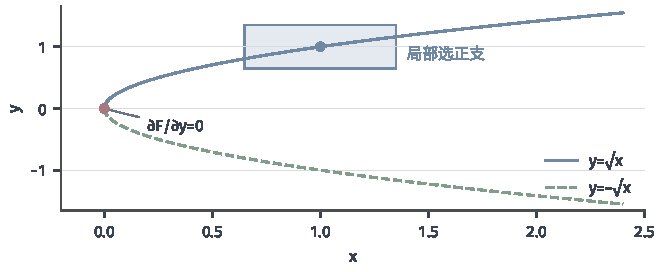
\includegraphics[width=112mm]{figures/00-shared/mathematical-preliminaries-upper/00-shared/matplotlib/mathematical-language-combinatorics-analysis-optimization-comprehension-additions/implicit-branches.pdf}
  \caption{方程$F(x,y)=y^2-x=0$的两支实数解。浅蓝矩形围住$(1,1)$，在该矩形内每个允许的$x$只有正支解，且$F_y=2y\neq0$；红点处$F_y=0$，两支相交。两支解满足同一方程，选定起始解与邻域才确定隐函数分支。}
  \label{fig:vol1-add-implicit-branches}
\end{figure}
\FloatBarrier


\paragraph{存在、唯一性与微分}

为什么条件是关于待解变量的导数可逆？先看线性方程。

设$\bm x\in\mathbb R^p$为参数、$\bm y\in\mathbb R^m$为未知量，$\bm P\in\mathbb R^{m\times p}$、$\bm Q\in\mathbb R^{m\times m}$固定，方程$\bm P\bm x+\bm Q\bm y=\bm 0$有$m$个方程、$m$个未知量。当$\bm Q$可逆时，对每个$\bm x$都有唯一解$\bm y=-\bm Q^{-1}\bm P\bm x$；$\bm Q$不可逆时，解要么不存在，要么不唯一。

对非线性方程$F(\bm x,\bm y)=\bm 0$，可微性说明它在基点附近近似于线性方程
\[
 \bm D_{\bm x}F(\bm a,\bm b)(\bm x-\bm a)+\bm D_{\bm y}F(\bm a,\bm b)(\bm y-\bm b)\approx\bm 0,
\]
其中$\bm D_{\bm x}F$、$\bm D_{\bm y}F$分别是只对$\bm x$、只对$\bm y$的坐标求偏导排成的Jacobian块。隐函数定理断言：只要线性近似中$\bm Q=\bm D_{\bm y}F$可逆，非线性方程在局部也像线性方程一样有唯一解，而且解的导数就是线性解的系数$-\bm Q^{-1}\bm P$。

隐函数定理给出的是充分条件：先保证局部解存在且唯一，再保证解随参数连续可微。
可逆性只要求待解变量对应的方阵Jacobian可逆，并不要求整个带参数映射的Jacobian是方阵。
\begin{theorem}[隐函数定理]
\label{thm:analysis-implicit-function}
设$F:\mathbb{R}^p\times\mathbb{R}^m\to\mathbb{R}^m$在$(\bm{a},\bm{b})$的某个开邻域内连续可微，$F(\bm{a},\bm{b})=\bm{0}$，并且关于待解变量的Jacobian矩阵
\[
 \bm{D}_{\bm{y}}F(\bm{a},\bm{b})\in\mathbb{R}^{m\times m}
\]
可逆。则存在$\bm{a}$与$\bm{b}$的邻域$U,V$，以及唯一的连续可微函数
$\varphi:U\to V$，使$\varphi(\bm{a})=\bm{b}$，并且对所有
$(\bm{x},\bm{y})\in U\times V$都有
\[
  F(\bm{x},\bm{y})=\bm{0}
  \quad\Longleftrightarrow\quad
  \bm{y}=\varphi(\bm{x}).
\]
其Jacobian矩阵满足
\begin{equation}
  \bm{D}\varphi(\bm{x})
  =
  -
  \bigl[\bm{D}_{\bm{y}}F(\bm{x},\varphi(\bm{x}))\bigr]^{-1}
  \bm{D}_{\bm{x}}F(\bm{x},\varphi(\bm{x})).
\label{eq:analysis-implicit-derivative}
\end{equation}
\end{theorem}
若已知$\varphi$存在且可微，导数公式可以直接由链式法则得到：对恒等式$F(\bm x,\varphi(\bm x))=\bm 0$求导，得$\bm D_{\bm x}F+\bm D_{\bm y}F\,\bm D\varphi=\bm 0$，再左乘$(\bm D_{\bm y}F)^{-1}$。定理真正困难的部分是$\varphi$的存在、唯一与可微，形式求导不能替代这些步骤。

证明的思路是把解方程改写为反复修正的迭代。一元时，固定$x$，从$y_0=b$出发，用$y_{n+1}=y_n-F(x,y_n)/F_y(a,b)$不断修正：若$F(x,y_n)>0$且$F_y(a,b)>0$，就把$y$调小一点。这类似Newton法，只是斜率固定用基点处的值。若每次修正都使误差按固定比例缩小，迭代就收敛到唯一解。
证明分别检查三件事：修正映射是压缩；它不把点送出所考察的球；所得解随参数可微。
\begin{proof}
为证明定理~\ref{thm:analysis-implicit-function}的存在性，先把方程改写为局部压缩迭代。记
\[
 \begin{gathered}
\bm{A}=\bm{D}_{\bm{y}}F(\bm{a},\bm{b})\\
T_{\bm{x}}(\bm{y})=\bm{y}-\bm{A}^{-1}F(\bm{x},\bm{y}).
 \end{gathered}
\]
因为$\bm A^{-1}$可逆，$F(\bm{x},\bm{y})=\bm{0}$当且仅当$T_{\bm{x}}(\bm{y})=\bm{y}$，即$\bm y$是更新后保持不变的点，称为不动点。并且
\[
 \bm{D}_{\bm{y}}T_{\bm{x}}(\bm{y})=\bm{I}-\bm{A}^{-1}\bm{D}_{\bm{y}}F(\bm{x},\bm{y}),
\]
它在$(\bm{a},\bm{b})$处为零。由$F$的导数连续，这个矩阵的元素在基点附近都很小；又由Cauchy--Schwarz不等式，算子范数不超过Frobenius范数。因而可以选择闭球$B=\{\bm{y}:\lVert\bm{y}-\bm{b}\rVert_2\leq r\}$和$\bm{a}$的邻域$U$，使
\begin{equation}
  \sup_{\bm{x}\in U,\,\bm{y}\in B}
  \left\lVert
    \bm{D}_{\bm{y}}T_{\bm{x}}(\bm{y})
  \right\rVert_{\mathrm{op}}
  \leq q<1.
\label{eq:analysis-ift-uniform-contraction}
\end{equation}
沿$\bm{y}$方向使用式~\eqref{eq:analysis-operator-mean-value-bound}（球是凸集，球内线段不离开球）可知，每个
$T_{\bm{x}}$都把$B$内任意两点之间的距离缩小到原来的至多$q$倍。

还必须核对自映射，即$T_{\bm x}$不把$B$中的点送出$B$；否则迭代可能离开压缩成立的范围。因为$T_{\bm{a}}(\bm{b})=\bm{b}$且$T_{\bm{x}}(\bm{b})$关于$\bm{x}$连续，可进一步缩小$U$，使
\[
 \lVert T_{\bm{x}}(\bm{b})-\bm{b}\rVert_2\leq\frac{1-q}{2}r.
\]
于是对$\bm{y}\in B$，先用三角不等式拆开，再用压缩性，
\[
 \begin{aligned}
  \lVert T_{\bm{x}}(\bm{y})-\bm{b}\rVert_2
  &\leq
  \lVert T_{\bm{x}}(\bm{y})-T_{\bm{x}}(\bm{b})\rVert_2+\lVert T_{\bm{x}}(\bm{b})-\bm{b}\rVert_2\\
  &\leq
  q\lVert\bm{y}-\bm{b}\rVert_2+\frac{1-q}{2}r
  \leq
  \frac{1+q}{2}r
  <r.
 \end{aligned}
\]
所以$T_{\bm{x}}(B)$包含在$B$的内部$V$中。
固定$\bm x\in U$，从$\bm y_0=\bm b$出发，令$\bm y_{n+1}=T_{\bm x}(\bm y_n)$。
所有迭代项都留在$B$内，每一步的压缩使相邻差满足
$\lVert\bm y_{n+1}-\bm y_n\rVert_2\leq q\lVert\bm y_n-\bm y_{n-1}\rVert_2\leq\cdots\leq q^n\lVert\bm y_1-\bm y_0\rVert_2$。
增大$q$仍保留这个上界，因而可设$0<q<1$。对$m>n$，几何和给出
\[
 \lVert\bm y_m-\bm y_n\rVert_2
 \leq\sum_{j=n}^{m-1}\lVert\bm y_{j+1}-\bm y_j\rVert_2
 \leq\frac{q^n}{1-q}\lVert\bm y_1-\bm y_0\rVert_2\longrightarrow0.
\]
每个坐标都是实柯西列，所以该序列在有限维欧氏空间中收敛；闭性使极限仍在$B$内。
$T_{\bm x}$连续，在$\bm y_{n+1}=T_{\bm x}(\bm y_n)$中令$n\to\infty$，可得极限$\varphi(\bm x)$满足
$T_{\bm x}(\varphi(\bm x))=\varphi(\bm x)$，而$T_{\bm x}(B)\subset V$使它属于$V$。
若另有不动点$\bm z\in B$，则
$\lVert\bm z-\varphi(\bm x)\rVert_2=\lVert T_{\bm x}(\bm z)-T_{\bm x}(\varphi(\bm x))\rVert_2\leq q\lVert\bm z-\varphi(\bm x)\rVert_2$，
由$q<1$只能有$\bm z=\varphi(\bm x)$，所以这个不动点唯一。若
$(\bm{x},\bm{y})\in U\times V$且$F(\bm{x},\bm{y})=\bm{0}$，则$\bm{y}\in B$也是
$T_{\bm{x}}$的不动点，唯一性迫使$\bm{y}=\varphi(\bm{x})$。这证明了定理所述的局部
存在与零点集合的逐点唯一性。

还需说明所得解随参数连续可微。先证$\varphi$局部Lipschitz连续，即它不会随参数剧烈变化。把$U$进一步缩小为开球，并使
$\overline U\times B$包含在原定义域内；这个集合闭且有界，$T_{\bm x}(\bm y)$关于$\bm x$的导数$-\bm A^{-1}\bm D_{\bm x}F$各分量连续，
故有统一范数上界$L$。对$\bm x,\bm x'\in U$，
两点间的线段仍在$U$内，式~\eqref{eq:analysis-operator-mean-value-bound}
可用于$T_{\bm x}(\bm y)$的参数变化。利用两个不动点关系$\varphi(\bm x)=T_{\bm x}(\varphi(\bm x))$、$\varphi(\bm x')=T_{\bm x'}(\varphi(\bm x'))$，把差拆成“改变$\bm y$”与“改变$\bm x$”两步：
\[
 \begin{aligned}
 \lVert\varphi(\bm{x})-\varphi(\bm{x}')\rVert_2
 &\leq\lVert T_{\bm x}(\varphi(\bm x))-T_{\bm x}(\varphi(\bm x'))\rVert_2\\
 &\quad+\lVert T_{\bm x}(\varphi(\bm x'))-T_{\bm x'}(\varphi(\bm x'))\rVert_2\\
 &\leq q\lVert\varphi(\bm{x})-\varphi(\bm{x}')\rVert_2+L\lVert\bm{x}-\bm{x}'\rVert_2,
 \end{aligned}
\]
移项得到$\lVert\varphi(\bm x)-\varphi(\bm x')\rVert_2
\leq L\lVert\bm x-\bm x'\rVert_2/(1-q)$，
故$\varphi$局部Lipschitz连续。

再证可微。令$\bm{h}\to\bm{0}$并记$\bm{k}=\varphi(\bm{x}+\bm{h})-\varphi(\bm{x})$，前述界给出$\lVert\bm{k}\rVert_2=O(\lVert\bm{h}\rVert_2)$。两点都在解集上，所以
\[
 F(\bm{x}+\bm{h},\varphi(\bm{x})+\bm{k})-F(\bm{x},\varphi(\bm{x}))=\bm{0}.
\]
对左侧作联合扰动$(\bm h,\bm k)$的一阶展开，得到
\[
 \bm{D}_{\bm{x}}F\,\bm{h}+\bm{D}_{\bm{y}}F\,\bm{k}+o(\lVert\bm{h}\rVert_2)=\bm{0}.
\]
展开中的Jacobian均在$(\bm x,\varphi(\bm x))$处取值，联合扰动的余项
$o(\lVert(\bm h,\bm k)\rVert_2)$因$\lVert\bm k\rVert_2=O(\lVert\bm h\rVert_2)$
成为$o(\lVert\bm h\rVert_2)$。
基点的$\det\bm A\neq0$，行列式又是矩阵元素的连续函数，
所以邻域足够小时$\bm D_{\bm y}F$仍可逆。左乘它的逆，得到
\[
 \bm{k}=-(\bm{D}_{\bm{y}}F)^{-1}\bm{D}_{\bm{x}}F\,\bm{h}+o(\lVert\bm{h}\rVert_2).
\]
这证明$\varphi$可微并给出式~\eqref{eq:analysis-implicit-derivative}；右侧各Jacobian矩阵及矩阵求逆都连续，又保证$\bm{D}\varphi$连续。至此，隐函数定理中的存在、局部唯一与导数公式都已得到证明。
\end{proof}

\paragraph{隐函数的导数}

定理的证明已同时建立解分支的存在、唯一性、可微性及式~\eqref{eq:analysis-implicit-derivative}。计算时只需在选定分支上代入两个Jacobian。用示例~\ref{ex:multivariable-implicit-parabola-branches}和示例~\ref{ex:multivariable-implicit-circle}的方程，可以核对不同分支各自的变化率。

\begin{example}[隐函数分支的导数]
设$F(x,y)=y^2-x$，在$(1,1)$处有$F=0$、$F_y=2\neq0$。
隐函数定理保证$(1,1)$附近的解可以唯一写成$y=\varphi(x)$，且
\[
 \begin{gathered}
\varphi'(x)=-\frac{F_x(x,\varphi(x))}{F_y(x,\varphi(x))}
 =\frac1{2\varphi(x)}\\
\varphi'(1)=\frac12.
 \end{gathered}
\]
直接选正支$\varphi(x)=\sqrt x$，求导同样得到$1/(2\sqrt x)$。
若在$(1,-1)$附近选负支，导数则为$-1/2$。

对单位圆$x^2+y^2=1$上半圆的一点$(x_0,y_0)$（$y_0>0$），同一公式给出$\varphi'(x_0)=-x_0/y_0$，不必先解出$y=\sqrt{1-x^2}$。
\end{example}

起始解不同，所追踪的函数也不同，导数公式要在选定分支上取值。单位圆的导数$-x_0/y_0$在$y_0\to0$时趋于无穷，与$(1,0)$处的竖直切线相符，也与示例~\ref{ex:multivariable-implicit-circle}中$(1,0)$附近不能把$y$解成$x$的函数相一致。

\subsection{特征值与特征向量的局部微分}

隐函数定理也能研究矩阵变化时的特征方向。设实对称矩阵$\bm S_0\in\mathbb R^{d\times d}$有一个简单特征值$\lambda_0$，对应单位特征向量$\bm v_0$。简单表示这个特征值的代数重数为$1$；对实对称矩阵，这等价于其特征空间是一维的。即使规定向量长度为$1$，$\bm v_0$和$-\bm v_0$仍代表同一方向；为了在局部选定一支，我们要求附近的向量$\bm v$满足$\bm v_0^\top\bm v>0$。

把对称矩阵$\bm S$作为参数，选取其上三角元素作为独立坐标，便可把对称矩阵空间视为有限维欧氏空间。把向量$\bm v$和标量$\lambda$作为未知量。特征方程与单位长度条件合起来写成
\[
 F(\bm S,\bm v,\lambda)=
 \begin{pmatrix}\bm S\bm v-\lambda\bm v\\ (\bm v^\top\bm v-1)/2\end{pmatrix}=\bm0.
\]
在$(\bm S_0,\bm v_0,\lambda_0)$处，关于$(\bm v,\lambda)$的导数作用于$(\bm h,\eta)$，其矩阵为
\[
 \begin{pmatrix}\bm S_0-\lambda_0\bm I&-\bm v_0\\
 \bm v_0^\top&0\end{pmatrix}.
\]
若该矩阵把$(\bm h,\eta)$映为零，先用$\bm v_0^\top$左乘第一行，利用对称性及$\bm S_0\bm v_0=\lambda_0\bm v_0$得到$\eta=0$；第二行给出$\bm v_0^\top\bm h=0$。此时$\bm h$既属于$\lambda_0$的特征空间，又与$\bm v_0$正交。由于特征值简单，只能有$\bm h=\bm0$。因此这个方阵可逆，隐函数定理保证在$\bm S_0$附近存在可微的特征值和单位特征向量分支；上述内积为正的条件固定了局部符号。

对称扰动方向$\bm E$使特征值与特征向量分别产生一阶变化$\dot\lambda$和$\dot{\bm v}$。对特征方程与归一化条件求微分，并在基点取值，得到
\[
 \begin{gathered}
(\bm S_0-\lambda_0\bm I)\dot{\bm v}
 =-(\bm E-\dot\lambda\bm I)\bm v_0\\
\bm v_0^\top\dot{\bm v}=0.
 \end{gathered}
\]
用$\bm v_0^\top$左乘第一式，便得到$\dot\lambda=\bm v_0^\top\bm E\bm v_0$。把它代回后，右侧与$\bm v_0$正交；由于$\lambda_0$简单，$\bm S_0-\lambda_0\bm I$限制在$\bm v_0$的正交补上可逆，因此第二式选出了唯一的$\dot{\bm v}$。

这里的结论依赖所选特征值简单。重特征值使上述关于未知量的导数失去可逆性，因此不能直接用这个构造；这并不意味着每一条特征值分支都不可微。研究重根附近时，可以改为考察相应特征子空间，而不是强行指定其中某一个特征向量。


\subsection{局部反函数与坐标变换}

另一个常见问题是反求输入：已知映射$G$的输出$\bm y$，能否唯一确定产生它的输入$\bm x$，并且$\bm x$随$\bm y$光滑变化。例如由直角坐标$(x,y)$反求极坐标$(r,\theta)$。
线性映射$\bm y=\bm M\bm x$可逆当且仅当方阵$\bm M$可逆；非线性映射在一点附近近似于它的Jacobian，所以可以期待：Jacobian可逆时，映射在局部可逆。
把$G(\bm x)-\bm y=\bm 0$看成以输出为参数、输入为待解变量的一组方程，就能使用隐函数定理。
定理只给出两个邻域之间的逆映射，不断言$G$在整个定义域上单射。
\begin{theorem}[局部反函数定理]
\label{thm:multivariable-inverse-function}
设$U\subseteq\mathbb R^d$开，$G:U\to\mathbb R^d$连续可微，$\bm a\in U$，且$\bm J_G(\bm a)$可逆。
则存在$\bm a$的开邻域$U_0$与$G(\bm a)$的开邻域$V_0$，使$G:U_0\to V_0$为双射，逆映射连续可微，并满足
\[
 \bm J_{G^{-1}}(G(\bm x))=[\bm J_G(\bm x)]^{-1}
 \qquad(\bm x\in U_0).
\]
\end{theorem}
\begin{proof}
以输出$\bm y$为参数、原输入$\bm x$为待解变量，令$H(\bm y,\bm x)=G(\bm x)-\bm y$。
在$(G(\bm a),\bm a)$处，关于$\bm x$的Jacobian就是可逆的$\bm J_G(\bm a)$。隐函数定理给出开邻域$V_0$、$W$以及$C^1$映射$\varphi:V_0\to W$，使
\[
 G(\bm x)=\bm y\quad\Longleftrightarrow\quad\bm x=\varphi(\bm y)
 \qquad(\bm y\in V_0,\ \bm x\in W).
\]
将$W$缩小并重新选取$V_0$，可使$W\subset U$且$\bm J_G$在$W$内均可逆。
令$U_0=W\cap G^{-1}(V_0)$，它因$G$连续而为包含$\bm a$的开集。
每个$\bm y\in V_0$都有$G(\varphi(\bm y))=\bm y$，故$\varphi(\bm y)\in U_0$；反之，每个$\bm x\in U_0$都由上述唯一性满足$\varphi(G(\bm x))=\bm x$。
因此$G:U_0\to V_0$为双射，逆就是$C^1$映射$\varphi$。
对$G(\varphi(\bm y))=\bm y$使用链式法则，得到$\bm J_G(\varphi(\bm y))\bm J_\varphi(\bm y)=\bm I$，左乘逆矩阵便得到所述公式。
\end{proof}
公式说明，逆映射的局部伸缩恰好抵消原映射的局部伸缩。极坐标映射可以具体说明这一点。
\begin{example}[极坐标的局部反函数]
\label{ex:multivariable-polar-local-inverse}
对$P(r,\theta)=(r\cos\theta,r\sin\theta)^\top$，示例~\ref{ex:multivariable-polar-jacobian}算得$\det\bm J_P=r$，所以在$r>0$的每一点附近，都可以从$(x,y)$唯一、光滑地反求$(r,\theta)$。在$(r,\theta)=(2,\pi/2)$，即平面上的点$(0,2)$处，
\[
\begin{gathered}
\bm J_P=\begin{bmatrix}0&-2\\1&0\end{bmatrix}\\
\bm J_{P^{-1}}(0,2)=\bm J_P^{-1}=\begin{bmatrix}0&1\\-1/2&0\end{bmatrix}.
\end{gathered}
\]
第一行说明$\mathrm dr=\mathrm dy$：在正上方的点，向上移动直接增大半径。第二行说明$\mathrm d\theta=-\mathrm dx/2$：向左移动使角度增大，且因为半径为$2$，角度变化只有水平位移的一半。
\end{example}

在原点$r=0$处，Jacobian行列式为零，所有$\theta$都映到同一点，确实无法反求$\theta$；这正是定理条件不满足的地方。

\paragraph{局部可逆与整体单射}

Jacobian处处可逆仍不保证映射在整个定义域上单射。
\begin{example}[Jacobian处处可逆而不单射]
\label{ex:multivariable-local-not-global-inverse}
考虑映射
\[
\begin{gathered}
g(u,v)=(e^u\cos v,e^u\sin v)^\top\\
(u,v)\in\mathbb R^2.
\end{gathered}
\]
它的Jacobian矩阵为
\[
\begin{gathered}
\bm J_g(u,v)=\begin{bmatrix}e^u\cos v&-e^u\sin v\\ e^u\sin v&e^u\cos v\end{bmatrix}\\
\det\bm J_g=e^{2u}>0,
\end{gathered}
\]
处处可逆。但$(u,v)$与$(u,v+2\pi)$给出同一输出，$g$不是单射。
\end{example}

这个$g$就是半径取$e^u$的极坐标映射：在每一点附近可以反求，整个平面上的输入却绕着原点重复覆盖输出。

另一方面，存在连续逆也不保证逆可微：一元函数$x\mapsto x^3$全局单射，其逆$y\mapsto y^{1/3}$在$0$处没有有限导数；这正对应$x^3$在$0$处导数为零，定理条件不满足。使用局部反函数定理时，需要逐项检查邻域、可微性和Jacobian的可逆性。

\FloatBarrier


\FloatBarrier
\section{本章小结}
\label{sec:multivariable-differentiation-summary}

多元极限要求所有趋近方式给出同一结果，只检查坐标轴或直线还不够。可微要求所有小扰动共用一个线性近似；偏导数或各方向导数存在，并不单独保证可微。梯度给出标量函数的一阶变化，Jacobian矩阵记录向量值映射的微分，Hessian矩阵描述二阶变化，并在相应条件下帮助判断驻点附近的形状。

矩阵微分保留输入和输出的形状，也保留矩阵乘法次序。对求逆、行列式和对数行列式，微分给出一阶扰动预测；要控制有限扰动的误差，还须核对定义域和余项界。隐函数与反函数定理说明，在选定基点且相关Jacobian可逆时，方程或映射在邻域中确定可微分支；这种局部结论不能替代全局唯一性。

\chapter{多元函数积分}
\label{chap:multivariate-integration}

累计范围由区间变成平面区域、空间曲线或曲面时，需要分别确定每个小块的体积、长度或面积；计算做功和通量时，还须记录行进方向或法向。本章建立这些积分并比较它们所累计的对象，再研究内部变化和边界累计之间的关系。

区域积分承接一元Riemann积分，先建立Jordan区域上的分割和，再讨论累次积分、换元和参数积分。路径积分与曲面积分分别使用弧长和面积，也讨论带方向的功与通量。最后，Green、Gauss和Stokes公式把区域或曲面内部的导数累计与其边界上的累计联系起来；使用每个公式时都要核对光滑性、可积性和方向条件。

\section{区域积分的定义与性质}
\label{sec:multivariable-region-integration}

一块不均匀的金属薄片占据平面区域$D$，在点$(x,y)$附近每单位面积的质量为$\rho(x,y)$。
把$D$切成许多小块，每块的质量约等于块内某一点的密度乘这块的面积；把所有小块的质量相加，就得到总质量的近似值，小块切得越细，近似越准确。
空间物体的质量、带电体的总电荷也按同样方式累计，只是面积换成体积，面密度换成体密度或电荷密度。
这类问题中的被积函数都是多元标量函数$f:D\subseteq\mathbb R^d\to\mathbb R$：输入是一个位置的$d$个坐标，输出是该位置上一个待累计的数。

同一个积分还有两种常用读法。
若$f\geq0$定义在平面区域$D$上，积分等于以$D$为底、以$f$的图像为顶的立体的体积，这是一元积分“曲线下方面积”在高一维的对应。
当$D$的面积有限且非零时，把积分除以面积，所得的数是$f$在$D$上的平均值，例如一个地区的平均降雨量或一块薄板的平均温度。

本章从有界区域上的Riemann积分出发。先定义分割与累计，再用截面、坐标变换和参数求导组织计算。一般可测函数与积分极限定理在\BookChapterRef{chap:integration}{第~\ref{chap:integration}章}中建立，这里不以它们为前提。

\subsection{盒体积与Jordan区域}

闭坐标盒$Q=\prod_{j=1}^d[a_j,b_j]$的体积定义为$\operatorname{vol}(Q)=\prod_j(b_j-a_j)$。某条边长度为零时体积为零。

沿任意坐标把盒切成有限块，切开的边长相加仍等于原边长，因此小盒体积之和等于原体积；对有限网格反复应用便得到有限可加性，公共的盒边界不重复贡献体积。

对有界集合$D\subset\mathbb R^d$，用有限个内部互不相交的盒从内侧和外侧逼近$D$。若每个$\varepsilon>0$都能选取这样的内、外有限盒并，使外侧总体积与内侧总体积之差小于$\varepsilon$，称$D$为Jordan可测集合。这个共同逼近的极限称为$D$的Jordan体积，记为$|D|$。

体积不依赖所选网格：任取一组内逼近和另一组外逼近，前者体积不超过后者；当两侧差距可任意小时，能够夹住的数只有一个。

有界集合Jordan可测的等价条件是：其边界$\partial D$可被有限个总体积任意小的盒覆盖。边界以外的点或者有邻域完全落在$D$内，或者有邻域完全落在$D$外；因此同时接触$D$和其补集的网格小盒必与边界相交。

给定$\varepsilon>0$，先用有限个总体积小于$\varepsilon/2$的盒覆盖边界，再将每个盒的各边稍微向外扩张，使扩张后总体积仍小于$\varepsilon$。因为盒的个数有限，可选足够小的网格直径，使每个与边界相交的小盒都落入某个扩张盒。小盒内部互不重叠，故这些小盒的体积之和至多为扩张盒总体积，小于$\varepsilon$。

反过来，边界包含在外逼近减去内逼近的内部之后所剩的部分中；这部分除内外体积之差外，至多还包含有限个盒的边界。盒边界同样可用总体积任意小的有限盒覆盖，所以整个边界可被任意小体积覆盖。这一条件也解释了边界为何不影响累计：只要被积函数有界，落在边界附近的总贡献就被函数绝对值上界乘覆盖盒总体积控制。

例如闭圆盘是Jordan可测的。它的圆周可以分成有限条足够短的弧，每条弧用小正方形覆盖；当弧长尺度缩小时，所需正方形个数按尺度的倒数增长，而每个正方形面积按尺度的平方缩小，所以总面积趋于零。同理，有限条分片光滑曲线围成的平面区域，以及有限片光滑曲面围成的有界立体，其边界都能这样覆盖。这里依赖有限片及其足够规则的参数化，不能仅凭“看起来像曲线或曲面”就忽略任意复杂边界。

\subsection{多元Riemann和与可积性}

设$R$是包含$D$的闭坐标盒。沿各坐标作有限分割，得到小盒$Q_1,\ldots,Q_N$；网格大小是各小盒直径的最大值。在每个$Q_i$中任选取样点$\bm\xi_i$，对$R$上的有界函数$g$形成Riemann和
\[
 S(g,P,\bm\xi)=\sum_{i=1}^N g(\bm\xi_i)\operatorname{vol}(Q_i).
\]
若当网格大小趋于零时，不论如何选取分割和取样点，这些和都趋于同一个有限值，就称$g$在$R$上Riemann可积，公共极限记作$\int_R g(\bm x)\,\mathrm d\bm x$。

这一要求控制所有足够细的取样，而不是只检查某一种选点方式。

在每个小盒上分别取函数的上确界和下确界，乘盒体积并求和，得到上和$U(g,P)$和下和$L(g,P)$。任意取样和都位于二者之间；$g$可积当且仅当可以通过足够细的分割使$U(g,P)-L(g,P)$任意小。

若$g$在$R$上连续，紧性保证它一致连续；网格足够细时，每个小盒上的最大与最小函数值相差任意小，上下和的差便不超过这个差值乘$R$的体积，因此$g$可积。

对于有界Jordan可测的$D$和$D$上的有界函数$f$，令$g=f\mathbb I_D$，即在$R\setminus D$上取零。若$g$在$R$上Riemann可积，就把其积分定义为$\int_D f$。选择更大的包含盒只增加一片零延拓区域，不改变结果。

若$f$可以连续延拓到$\overline D$，则该延拓在闭包上一致连续。远离边界的小盒可用一致连续性控制振幅，靠近边界的小盒由前述有限盒覆盖控制总体积，所以零延拓可积。有限分块上分别连续、且不连续只落在这些分块可忽略边界上的有界函数，也可逐块使用同一论证。边界上怎样赋值不改变积分。

连续只是充分条件，不是必要条件。例如$R=[0,1]^2$上令$g(x,y)=\mathbb I_{\{x\geq1/2\}}$，它在直线$x=1/2$上不连续，但只有穿过该直线的网格小盒可能贡献上下和差；这些小盒的总面积随网格变细趋于零，因此$g$可积，其积分为$1/2$。

相反，有界本身不够：$\mathbb I_{\mathbb Q^2}$在每个非退化小盒内既取$0$也取$1$，上下和之差始终等于盒体积，因而不可积。

\subsection{积分的性质与累计量}

线性、单调性和绝对值估计都由有限Riemann和的对应性质取极限得到。例如若$f$、$h$可积且$f\leq h$，则$\int_D f\leq\int_D h$，并且$|\int_D f|\leq\int_D|f|$。有限个Jordan区域内部互不重叠，且拼接处落在可忽略的公共边界上时，分别求和再相加，得到区域可加性。

取$f=1$得到体积；非负密度$\rho$的积分是总质量，$|D|>0$时$|D|^{-1}\int_D f$是平均值；质量$M=\int_D\rho$有限且非零时，质心为$M^{-1}\int_D\bm x\rho(\bm x)\,\mathrm d\bm x$，向量积分按分量计算。

\section{累次积分}

区域积分的定义把所有坐标同时分割；计算时希望先沿一个方向累计，再沿其他方向累计。能否这样做，需要同时控制各截面的误差。

\subsection{长方体上的累次积分}

设$f$在闭矩形$R=[a,b]\times[c,d]$上连续。固定$x$时，一元积分$F(x)=\int_c^d f(x,y)\,\mathrm dy$存在。由于$f$在$R$上一致连续，当$x$变化足够小时，所有$y\in[c,d]$处的函数值同时变化很小，故$F$连续。

对乘积网格，把有限个取样和按列分组；内层求和趋于各列的$y$方向积分，一致连续性控制所有列的误差，外层求和再趋于$\int_a^bF(x)\,\mathrm dx$。按行分组同理，因而
\[
 \int_R f(x,y)\,\mathrm d(x,y)
 =\int_a^b\left(\int_c^d f(x,y)\,\mathrm dy\right)\mathrm dx
 =\int_c^d\left(\int_a^b f(x,y)\,\mathrm dx\right)\mathrm dy.
\]
这是一组容易核对的充分条件：一般Riemann可积函数的每个截面未必都可积，不能仅由整体可积就不检查内层积分。更多坐标的闭盒可重复上述分组。

\subsection{简单区域与积分次序的选择}

若$D=\{(x,y):a\leq x\leq b,\ \alpha(x)\leq y\leq\beta(x)\}$，边界函数$\alpha\leq\beta$连续，且$f$在$D$的闭包上连续，则
\[
 \int_D f(x,y)\,\mathrm d(x,y)
 =\int_a^b\left(\int_{\alpha(x)}^{\beta(x)}f(x,y)\,\mathrm dy\right)\mathrm dx.
\]
这是对零延拓作网格分组：边界曲线附近的格子总体积可任意小，其余格子按截面累计。连续边界与紧性保证截面端点随$x$一致变化，内层积分也随$x$连续。有限个这样的区域可逐块处理，公共边界不重复累计；换次序时须重新求出投影和截面。

例如$D=\{0\leq y\leq x\leq1\}$，取$f(x,y)=x+y$。固定$x$，截面为$0\leq y\leq x$，得到
\[
 \int_0^1\left(\int_0^x(x+y)\,\mathrm dy\right)\mathrm dx
 =\int_0^1\frac{3x^2}{2}\,\mathrm dx=\frac12.
\]
固定$y$时截面变为$y\leq x\leq1$，因此同一个量也等于
\[
 \int_0^1\left(\int_y^1(x+y)\,\mathrm dx\right)\mathrm dy
 =\int_0^1\left(\frac12+y-\frac{3y^2}{2}\right)\mathrm dy=\frac12.
\]
两个上下限来自同一三角形的不同截面，并不是把原积分符号机械交换。

换序还可能改变分块方式。例如区域$0\leq x\leq2$、$0\leq y\leq\min(x,2-x)$是一个三角形。先对$y$积分时，在$x=1$处分成两块；先对$x$积分则用$0\leq y\leq1$、$y\leq x\leq2-y$。以$f=1$核验，两种次序都给出面积$1$。上下限来自截面，而不是积分符号本身。

\subsection{截断、奇点与交换次序的边界}

无界区域或无界密度不能直接代入上面的有界Riemann和。可以先选一族有界Jordan区域$D_\varepsilon$，避开奇点或截去远处，并逐个检查$f$在每个截断区域上Riemann可积，再考察$\int_{D_\varepsilon}f$的极限。

只沿某一族截断得到极限，并不自动证明其他截断方式给出相同结果。

例如在$(0,1]^2$上取$f(x,y)=(x^2-y^2)/(x^2+y^2)^2$。对$0<\varepsilon<1$，先用$D_\varepsilon=[\varepsilon,1]\times[\varepsilon^2,1]$截断。每个截断矩形远离原点，$f$连续。

若暂把下边界改为$y=0$，先对$y$积分可得
\[
 \int_\varepsilon^1\left(\int_0^1 f(x,y)\,\mathrm dy\right)\mathrm dx
 =\int_\varepsilon^1\frac{\mathrm dx}{1+x^2}
 \longrightarrow\frac\pi4.
\]
被去掉的窄条上$|f(x,y)|\leq1/x^2$，其绝对积分不超过$\varepsilon^2\int_\varepsilon^1x^{-2}\,\mathrm dx\to0$，故$\int_{D_\varepsilon}f\to\pi/4$。交换两条边的截断速度，令$E_\varepsilon=[\varepsilon^2,1]\times[\varepsilon,1]$；由$f(y,x)=-f(x,y)$，所得极限是$-\pi/4$。两族矩形都逐渐填满同一区域$(0,1]^2$，却得到不同极限；因此这里没有与这两种截断方式无关的总量。


\section{区域积分的换元}
\label{sec:classical-change-variables}

圆盘用半径和角度描述比用两个直角坐标更简单。但坐标变化也会改变小块的面积或体积，不能只替换函数中的变量。前面已经知道线性映射把体积乘以行列式的绝对值；可微映射在足够小的区域内近似线性，换元公式正是把这些局部比例累计起来。

\subsection{局部体积变化与换元公式}

为了明确单次覆盖和边界条件，先在两个开集之间使用可微双射，再取其中的有界积分区域。
\begin{theorem}[经典区域积分的换元]
设$U,V\subseteq\mathbb R^d$为开集，$T:U\to V$为$C^1$双射，逆映射也为$C^1$。设$E\subset U$为紧Jordan区域，且$T(E)$也是Jordan区域。若$f$在$T(E)$上连续，则
\[
 \int_{T(E)}f(\bm x)\,\mathrm d\bm x
 =\int_E f(T(\bm u))|\det DT(\bm u)|\,\mathrm d\bm u.
\]
\end{theorem}

先说明公式中的权重。对$E$附近等边网格中的小立方体，连续可微性给出统一的一阶近似
\[
 T(\bm u+\bm h)-T(\bm u)=DT(\bm u)\bm h+\bm R_{\bm u}(\bm h).
\]
当$\|\bm h\|\leq\delta$时，余项满足$\|\bm R_{\bm u}(\bm h)\|\leq\eta(\delta)\|\bm h\|$，其中$\eta(\delta)\to0$，并且这个界在紧集上对$\bm u$一致。逆导数同样有界，所以局部小盒不会在某一方向被任意压扁。

在线性像平行多面体的边界外加厚度与$\eta(\delta)\delta$同阶的薄层，就能夹住小盒的像；薄层体积相对于原盒体积趋于零。这给出局部体积比趋于$|\det DT(\bm u)|$。把像分割上的取样和与参数小盒上的加权取样和比较，连续函数的一致连续性控制函数值替换误差，前述统一余项控制体积误差，Jordan边界条件控制边界小块，取极限得到公式。

这是证明的局部分割思路；仅写出某一点的线性近似，尚不足以交换整个分割和的极限。

逆函数定理只保证每一点附近可以反解，并不保证整个区域只覆盖一次。上面的全局双射条件正是防止重复累计；行列式绝对值消除的是定向符号，不能消除覆盖次数。

\subsection{极坐标、柱坐标与球坐标}

平面极坐标将$(r,\theta)$送到$(r\cos\theta,r\sin\theta)$，Jacobian行列式为$r$。同一角度宽度在半径较大处扫过更长的弧，所以参数矩形的面积不能直接当作平面小块的面积。其面积权重是
\[
 \mathrm dA=r\,\mathrm dr\,\mathrm d\theta.
\]

\begin{figure}[!htb]
\centering
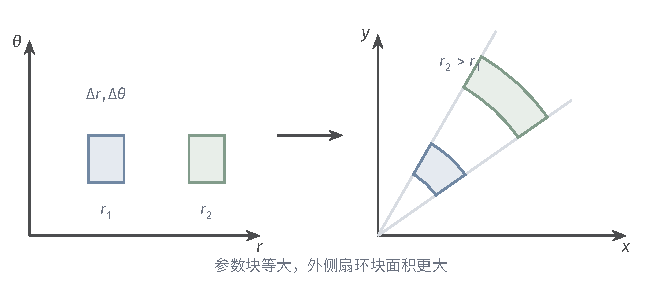
\includegraphics[width=112mm]{figures/00-shared/mathematical-preliminaries-upper/00-shared/tikz/mathematical-language-combinatorics-analysis-optimization-comprehension-additions/polar-area-weight.pdf}
\caption{同样的径向宽度和角度宽度，在较大半径处产生更大的面积。一阶面积为$r\Delta r\Delta\theta$，由此得到极坐标权重。}
\label{fig:vol3-classical-polar-weight}
\end{figure}

原点处行列式为零，角度的两端又表示同一条射线，因此不能把闭参数矩形直接代入上述双射定理。可以先限制$r\geq\varepsilon$且$\varepsilon\leq\theta\leq2\pi-\varepsilon$，在紧截断区域上换元，再令$\varepsilon\downarrow0$。对于圆盘上的连续函数，被去掉的小圆盘和窄扇区的贡献受函数上界乘面积控制，趋于零；参数侧的遗漏也由有界权重控制。

例如半径$R$的圆盘面积为
\[
 \int_0^{2\pi}\int_0^R r\,\mathrm dr\,\mathrm d\theta=\pi R^2.
\]
若角度取到$4\pi$，内部被覆盖两次，结果也变成两倍。对于有奇点的被积函数，不能只用“接缝不贡献面积”来跳过极限估计。

柱坐标保留高度$z$，即在极坐标后加上第三个坐标，其体积权重仍含$r$：
\[
 \mathrm dV=r\,\mathrm dr\,\mathrm d\theta\,\mathrm dz.
\]
因此半径$R$、高度$H$的圆柱体积为$\pi R^2H$。轴线和角度接缝通过与极坐标相同的截断处理。

球坐标使用距原点的距离$\rho$、从正$z$轴量起的极角$\varphi$和方位角$\theta$：
\[
 T(\rho,\varphi,\theta)
 =(\rho\sin\varphi\cos\theta,\rho\sin\varphi\sin\theta,\rho\cos\varphi).
\]
三个局部正交方向的长度比例分别是$1$、$\rho$和$\rho\sin\varphi$，也可直接计算Jacobian行列式验证。因此
\[
 \mathrm dV=\rho^2\sin\varphi\,\mathrm d\rho\,\mathrm d\varphi\,\mathrm d\theta.
\]

在$\rho>0$、$0<\varphi<\pi$及一个长度为$2\pi$的开角度区间内，映射单次覆盖去掉轴线和接缝后的空间。计算球内连续函数的积分时，先截去原点、极轴附近及接缝附近的小区域，再以有界性估计遗漏。球体积由此为
\[
 \int_0^{2\pi}\int_0^\pi\int_0^R
 \rho^2\sin\varphi\,\mathrm d\rho\,\mathrm d\varphi\,\mathrm d\theta
 =\frac{4\pi R^3}{3}.
\]

\subsection{线性换元与积分结果的核对}

线性变换可以把斜区域变成坐标盒。

设$D$由$0\leq x+y\leq2$和$0\leq x-y\leq2$围成，求$\int_D(x+y)\,\mathrm d(x,y)$。令$u=x+y$、$v=x-y$，则参数区域为$[0,2]^2$，逆变换为
\[
 x=(u+v)/2,
\]
\[
 y=(u-v)/2.
\]
其行列式为$-1/2$，故面积权重为$1/2$。于是
\[
 \int_D(x+y)\,\mathrm d(x,y)
 =\int_0^2\int_0^2\frac u2\,\mathrm du\,\mathrm dv=2.
\]
取被积函数为$1$，同样得到区域面积$2$；原被积函数在对称区域上的平均值为$1$，两者相乘也为$2$。这同时核验了区域、权重和积分值。

\section{参数积分}

若密度或被积函数还依赖一个参数，积分便定义了新的函数。

判断它是否连续、能否求导，需要控制整个积分区域上的变化，逐点成立的极限本身不够。本节固定紧Jordan区域$D$，用连续性提供统一控制。

\subsection{固定区域上的参数积分与连续性}

设$K$为紧参数区域，$f$在$D\times K$上连续，记
\[
 F(\bm t)=\int_D f(\bm x,\bm t)\,\mathrm d\bm x.
\]
乘积紧集上的一致连续性使$\sup_{\bm x\in D}|f(\bm x,\bm t)-f(\bm x,\bm s)|$在$\bm t\to\bm s$时趋于零。因此
\[
 |F(\bm t)-F(\bm s)|
 \leq |D|\sup_{\bm x\in D}|f(\bm x,\bm t)-f(\bm x,\bm s)|\longrightarrow0.
\]
这证明了连续性。参数区域不必整体有界：讨论一个内点附近时，取包含该点的小闭盒即可。

\subsection{积分号下的偏导数与全微分}

现在设参数属于开集，$f$和各参数偏导$\partial_{t_j}f$在$D$与参数邻域的乘积上连续。固定一个参数点和足够小的闭邻域，一元中值定理把差商写成附近参数处的偏导值。偏导的一致连续性说明差商对全部$\bm x\in D$一致趋于$\partial_{t_j}f$；对差取积分并用上面的上确界估计，便得到
\begin{equation}
 \partial_{t_j}F(\bm t)=\int_D\partial_{t_j}f(\bm x,\bm t)\,\mathrm d\bm x.
\label{eq:classical-differentiate-under-integral}
\end{equation}
右侧又是连续参数积分，故所有参数偏导连续，$F$是$C^1$函数。它的全微分为
\[
 DF_{\bm t}[\bm h]=\int_D D_{\bm t}f(\bm x,\bm t)[\bm h]\,\mathrm d\bm x.
\]

这里先获得偏导，再由连续偏导判据得到整体可微；不能只证明每个方向上的极限就略去这一步。

例如$F(t)=\int_0^1 e^{tx}\,\mathrm dx$，在任意有界参数区间上都满足这些条件，故$F'(0)=\int_0^1x\,\mathrm dx=1/2$，无需在$t=0$处处理显式表达式的可去奇点。

\subsection{变限参数积分}

积分区间也随参数变化时，积分值的变化有两部分：原区间内部函数改变，以及两端新添或移除的细条。

设$a(t),b(t)$为$C^1$函数，$f(x,t)$及$\partial_tf(x,t)$在所需区间附近连续。将积分写为固定基点到$b(t)$的积分减去固定基点到$a(t)$的积分，再用链式法则，得到
\[
 \frac{\mathrm d}{\mathrm dt}\int_{a(t)}^{b(t)}f(x,t)\,\mathrm dx
 =\int_{a(t)}^{b(t)}\partial_tf(x,t)\,\mathrm dx
 +f(b(t),t)b'(t)-f(a(t),t)a'(t).
\]

上端向右移动增加积分，下端向右移动减少积分，所以两个边界项符号相反。多个参数时逐一求偏导，或将$a'$、$b'$和$\partial_tf$换成作用于同一参数增量的全微分。更一般的移动区域会产生沿边界的贡献；本章只在上述区间变限和已明确参数化的区域上使用这一规则。

\par\Needspace{10\baselineskip}
\section{路径积分}
\label{sec:multivariable-path-integration}

区域积分累计的是铺满一块区域的量，许多问题却只沿一条曲线累计。一根弯曲细铁丝的质量由各处的线密度和铁丝长度决定；把物体沿一条路线推过去，推力做的功不仅取决于力的大小和路线长度，还取决于力与前进方向的夹角。
两类问题都沿曲线累计，被积对象却不同：线密度在每一点只给出一个数，是标量函数；力在每一点给出一个带方向的量，是向量场。

相应地有两种路径积分。第一类路径积分把曲线切成小段，用每段上的函数值乘这段的实际长度再相加，铁丝质量就是这样算出的；它不关心沿哪个方向走过曲线。
第二类路径积分在每一小段上先取力与这段有向位移的内积，只保留力沿前进方向的分量，再把这些数相加；反向行走时每段位移都反号，积分也随之变号。

两种积分都要先用参数描述曲线，因此本节先说明路径与弧长，再分别讨论两类积分的定义、性质和计算。
最后研究力沿路径做的功什么时候只取决于起点和终点、而与中间的路线无关，这对应物理中保守力与势能的关系。
本节的参数积分都是一元Riemann积分\scite{math-openstax-calculus3}。

\subsection{参数路径与弧长}
\label{sec:multivariable-line-integrals}

描述一次行进，需要知道每个时刻所在的位置。位置随时间连续变化，就得到一条路径；位置对时间的导数是速度，速度的大小称为速率。速率恒定时，速率乘经过的时间就是走过的路程。
本小节先给出路径的定义，再用折线逼近说明：速率随时间变化时，路程等于速率对时间的积分。

\subsubsection{路径的定义}

\paragraph{参数化路径}

不妨把参数$t$看成时间，把$\gamma(t)$看成一个质点在时刻$t$所在的位置。同一组位置可以走得快或慢，可以从任一端出发，也可以来回走好几遍；只记下经过了哪些点，就会丢失这些信息。

用区间到空间的连续映射描述行进过程，位置和先后次序就一起保留了下来。
\begin{definition}[路径]
设$a<b$。连续映射$\gamma:[a,b]\to\mathbb R^d$称为一条\term{路径}（path），$\gamma(a)$和$\gamma(b)$分别为起点和终点；若两者相等，称为闭路径。
集合$C=\gamma([a,b])$称为路径的像。
\end{definition}

像集$C$只记录质点经过的位置，参数$t$还规定了经过的先后次序，所以同一个像集可以对应行进方式完全不同的路径。
\begin{example}[同一条对角线段上的三条路径]
\label{ex:analysis-diagonal-segment-paths}
以下三条平面路径的像都是连接$(0,0)$与$(1,1)$的对角线段：
\begin{itemize}
 \item $\gamma(t)=(t,t)^\top$，$0\leq t\leq1$，从$(0,0)$走到$(1,1)$，速度为$(1,1)^\top$；
 \item $\eta(u)=(u/2,u/2)^\top$，$0\leq u\leq2$，同样从$(0,0)$走到$(1,1)$，速度减半为$(1/2,1/2)^\top$，用时加倍；
 \item $\rho(t)=(t,t)^\top$（$0\leq t\leq1$）、$\rho(t)=(2-t,2-t)^\top$（$1\leq t\leq2$），先走到$(1,1)$再原路返回。
\end{itemize}
$\gamma$与$\eta$只是快慢不同，线段上每个点都恰好经过一次。$\rho$的像仍是这条线段，但每个内点被经过两次：去程一次，回程一次。
\end{example}

后面会看到，两种路径积分对$\gamma$与$\eta$都给出相同结果；沿$\rho$按长度累计时，结果是沿$\gamma$的两倍，按有向位移累计时，去程与回程恰好抵消。
可见路径积分是沿“一次行进”定义的，只知道像集还不能确定它。要计算一根铁丝的质量，应选一条把铁丝恰好走一遍的路径。

\paragraph{分段光滑路径}

示例~\ref{ex:analysis-diagonal-segment-paths}中的往返路径$\rho$在$t=1$处突然掉头，正方形边界在四个角处突然转向。这些位置没有唯一的切线方向，但在每一段直线上速度都存在且连续。为了把折线、多边形边界这类常见路径纳入计算，允许路径在有限个参数点处分段。
\begin{definition}[分段光滑路径]
若存在分割$a=t_0<t_1<\cdots<t_n=b$，使$\gamma$在每个$[t_{j-1},t_j]$上为$C^1$映射，称$\gamma$为分段$C^1$路径，也称分段光滑路径。
若每段内部还满足$\gamma'(t)\neq\bm0$，称该路径分段正则。
\end{definition}

这里“在闭区间$[t_{j-1},t_j]$上为$C^1$”是指该段内部的导数连续，并能连续延拓到该段的两个端点；相邻两段在公共端点处的导数不必相同。
例如$\rho$在$[0,1]$上的速度为$(1,1)^\top$，在$[1,2]$上的速度为$(-1,-1)^\top$。两段在$t=1$处的速度不同，但各自连续，所以$\rho$是分段$C^1$路径。

本节的路径积分都在分段$C^1$路径上定义。折点只有有限个，而改变有界函数在有限个点的取值不影响Riemann积分，所以折点处的速度取什么值不影响参数积分。
分段正则要求每段内部速度不为零，排除了质点在某段中途停住的情形。本节的积分并不要求路径正则；后面用到单位切向量时，只在速度非零处使用它。

\subsubsection{路径的长度}

\paragraph{弧长}

测量一条弯曲道路的长度时，可以在路上依次插几根标杆，量出相邻标杆之间的直线距离再相加。每段直线距离都不超过对应那段路的实际长度，所以这样得到的折线长度不会超过道路长度；在两根标杆之间再插一根，由三角不等式，新折线的长度不会变短。标杆越密，折线越贴近道路，因此把实际长度定义为所有内接折线长度的上确界。
\begin{definition}[路径的弧长]
路径$\gamma:[a,b]\to\mathbb R^d$的弧长定义为
\[
 \ell(\gamma)=\sup_{a=t_0<\cdots<t_n=b}
 \sum_{j=1}^n\lVert\gamma(t_j)-\gamma(t_{j-1})\rVert_2.
\]
上确界取遍$[a,b]$的全部有限分割；若此值有限，称路径可求长。
\end{definition}

这个定义只用到路径上点的位置，不需要导数，所以任何连续路径都可以讨论它是否可求长。

对分段光滑路径，弧长还可以用速度直接计算。在一小段参数区间$[t_{j-1},t_j]$上，质点的位移近似为速度乘时间：
$\gamma(t_j)-\gamma(t_{j-1})\approx\gamma'(t_{j-1})(t_j-t_{j-1})$，
所以这一小段的长度近似为速率$\lVert\gamma'(t_{j-1})\rVert_2$乘时间，汽车里程表正是这样累计路程的。把这些乘积相加并令分割变细，就得到下面的公式。
\begin{theorem}[分段光滑路径的弧长]
若$\gamma:[a,b]\to\mathbb R^d$分段$C^1$，则它可求长，且
\[
 \ell(\gamma)=\int_a^b\lVert\gamma'(t)\rVert_2\,\mathrm dt.
\]
\end{theorem}
\begin{proof}
加入分点不会使折线变短，所以计算上确界时只需考虑包含全部折点的分割；这样的折线长度按光滑段相加，弧长也按段相加。因此只需在一段$C^1$区间上证明，再把各段的等式相加。证明分两步：先说明任何折线都不比速度积分长，再说明足够细的折线与速度积分相差任意小。

第一步。对该段中的$\alpha<\beta$，由各坐标分量的一元基本定理，
$\gamma(\beta)-\gamma(\alpha)=\int_\alpha^\beta\gamma'(t)\,\mathrm dt$，这里向量的积分表示对各分量分别积分。
若弦$\gamma(\beta)-\gamma(\alpha)$非零，取它方向上的单位向量$\bm u$，则由Cauchy--Schwarz不等式
\[
 \lVert\gamma(\beta)-\gamma(\alpha)\rVert_2
 =\bm u^\top\bigl(\gamma(\beta)-\gamma(\alpha)\bigr)
 =\int_\alpha^\beta\bm u^\top\gamma'(t)\,\mathrm dt
 \leq\int_\alpha^\beta\lVert\gamma'(t)\rVert_2\,\mathrm dt;
\]
弦为零时这个不等式直接成立。同样的推理说明，任何连续向量值函数$\bm v$都满足$\lVert\int_\alpha^\beta\bm v\,\mathrm dt\rVert_2\leq\int_\alpha^\beta\lVert\bm v\rVert_2\,\mathrm dt$。
对任意分割把各段弦长相加，可知任意内接折线的长度都不超过$\int_a^b\lVert\gamma'\rVert_2\,\mathrm dt$，所以上确界也不超过它。

第二步。$\gamma'$在紧区间上一致连续。给定$\varepsilon>0$，取足够细的分割，使每个小区间上任意两点的$\gamma'$相距小于$\varepsilon$，并记$\Delta t_j=t_j-t_{j-1}$。
在第$j$个小区间上，
\[
 \gamma(t_j)-\gamma(t_{j-1})-\gamma'(t_{j-1})\Delta t_j
 =\int_{t_{j-1}}^{t_j}\bigl(\gamma'(t)-\gamma'(t_{j-1})\bigr)\,\mathrm dt,
\]
由第一步的范数不等式，它的范数不超过$\varepsilon\Delta t_j$；于是这一段的弦长与$\lVert\gamma'(t_{j-1})\rVert_2\Delta t_j$之差不超过$\varepsilon\Delta t_j$。
同一小区间上，$\int\lVert\gamma'\rVert_2\,\mathrm dt$与$\lVert\gamma'(t_{j-1})\rVert_2\Delta t_j$的差也不超过$\varepsilon\Delta t_j$。
两项相加后对$j$求和，速度积分与这条折线长度的差不超过$2\varepsilon(b-a)$，所以上确界不小于速度积分减$2\varepsilon(b-a)$。令$\varepsilon\downarrow0$，得到反向不等式。
\end{proof}

用这个公式可以计算示例~\ref{ex:analysis-diagonal-segment-paths}中三条路径的长度，并检验圆周长公式。
\begin{example}[对角线段与圆周的弧长]
对角线段$\gamma(t)=(t,t)^\top$，$0\leq t\leq1$，速度为$(1,1)^\top$，速率为$\sqrt2$，所以$\ell(\gamma)=\int_0^1\sqrt2\,\mathrm dt=\sqrt2$。两个坐标各变化$1$，走过的距离却不是$1+1=2$，而是斜边的长度。

慢速路径$\eta$的速率为$\sqrt2/2$，用时为$2$，长度为$\int_0^2(\sqrt2/2)\,\mathrm du=\sqrt2$。往返路径$\rho$在两段上的速率都是$\sqrt2$，总用时为$2$，长度为$2\sqrt2$。

半径为$r$的圆周可以参数化为$t\mapsto(r\cos t,r\sin t)^\top$，$0\leq t\leq2\pi$。速度为$(-r\sin t,r\cos t)^\top$，速率恒为$r$，长度为$\int_0^{2\pi}r\,\mathrm dt=2\pi r$，与圆周长公式一致。
\end{example}

$\gamma$与$\eta$的长度相同，因为速率减半恰好被用时加倍抵消；$\rho$的长度是$\gamma$的两倍，因为弧长把经过的次数也计算在内。

记$s(t)=\int_a^t\lVert\gamma'(u)\rVert_2\,\mathrm du$为截至时刻$t$累计走过的路程，它就是里程表在时刻$t$的读数。在每个光滑段内部，$s$对$t$的导数是速率$\lVert\gamma'(t)\rVert_2$，因此常把长度权重简写为
$\mathrm ds=\lVert\gamma'(t)\rVert_2\,\mathrm dt$，读作“一小段时间$\mathrm dt$内走过的一小段路程”。

\subsection{第一类路径积分}

第一类路径积分的被积对象是定义在曲线上的标量函数，例如铁丝各处的线密度或一条道路沿线各处的温度。每一小段的贡献是函数值乘这一小段的实际长度，因此它只需要路程这一个权重，不涉及方向。

\subsubsection{定义与可积性}

\paragraph{按弧长的积分}

设一根铁丝沿路径$\gamma$放置，$h(\bm x)$是它在点$\bm x$处的线密度，即单位长度的质量。线密度为常数时，质量等于密度乘长度；密度随位置变化时，把铁丝切成许多小段，每段上的密度近似为常数。
在参数小区间$[t_{j-1},t_j]$对应的一段上取一个时刻$\xi_j$，这段的质量约为
\[
 h(\gamma(\xi_j))\,\lVert\gamma'(\xi_j)\rVert_2\,(t_j-t_{j-1}),
\]
即“该处密度”乘“该段长度”。把各段相加，就得到参数区间上函数$h(\gamma(t))\lVert\gamma'(t)\rVert_2$的积分和，所以用这个函数的一元积分定义沿路径的累计。这里先讨论沿路径连续的密度；有限分段连续的密度可逐段处理。
\begin{definition}[第一类路径积分]
设$\gamma:[a,b]\to\mathbb R^d$分段$C^1$，$h$在路径像集上连续。定义\term{第一类路径积分}为
\begin{equation}
 \int_\gamma h\,\mathrm ds=\int_a^b h(\gamma(t))\|\gamma'(t)\|_2\,\mathrm dt.
 \label{eq:analysis-scalar-line-integral}
\end{equation}
右侧按各光滑段的一元Riemann积分相加，因被积函数分段连续而存在。
\end{definition}

这个积分有几种常见读法。取$h=1$，积分就是弧长$\ell(\gamma)$；$h$是非负线密度时，积分是铁丝的总质量。

若$\ell(\gamma)>0$，比值
\[
 \bar h=\frac1{\ell(\gamma)}\int_\gamma h\,\mathrm ds
\]
是$h$沿曲线按长度的平均值：沿一条道路每隔相同路程记录一次温度再求平均，记录越密，结果越接近$\bar h$。
这里的平均按路程加权，而不按参数时间加权。若一辆车在某段路上开得很慢，按时间平均会让这段路的温度占更大比重，按路程平均则不受车速影响。

用一根密度不均匀的半圆铁丝可以说明质量和平均线密度的计算。
\begin{example}[上半圆铁丝的质量与平均线密度]
\label{ex:analysis-semicircle-wire}
沿上半单位圆$\gamma(t)=(\cos t,\sin t)^\top$，$0\leq t\leq\pi$，放一根铁丝，线密度为$h(x,y)=y$，即越高的地方越重。速度为$(-\sin t,\cos t)^\top$，速率恒为$1$，所以总质量为
\[
 \int_\gamma y\,\mathrm ds=\int_0^\pi\sin t\,\mathrm dt=2.
\]
铁丝长度为$\pi$，平均线密度为$\bar h=2/\pi\approx0.64$。两端$(\pm1,0)$处密度为零，顶点$(0,1)$处密度为$1$，平均值落在两者之间。
\end{example}
这条参数化的速率恒为$1$，参数时间与路程同步增长，所以按时间平均也得到$2/\pi$；速率不恒定时，两种平均一般不同。

连续密度在紧路径像集上有界，因而积分的绝对值不超过密度绝对值的上界乘弧长。路径积分按曲线上的实际取值累计，不能用区域平均值代替沿线的密度。

\subsubsection{积分的基本性质}

下面各条性质中的有符号函数都假设沿所讨论的路径可积。把定义式~\eqref{eq:analysis-scalar-line-integral}代入一元Riemann积分的相应性质，就逐项得到这些结论；用铁丝质量来读，每条性质都有直接的含义。

\paragraph{加法}

若$h,k$沿$\gamma$可积，则$h+k$也沿$\gamma$可积，且
\[
 \int_\gamma(h+k)\,\mathrm ds=\int_\gamma h\,\mathrm ds+\int_\gamma k\,\mathrm ds.
\]
绝对可积性由$|h+k|\leq|h|+|k|$保证，等式来自一元积分的加法。若铁丝由两种材料叠合而成，总质量等于两种材料各自的质量之和。

\paragraph{减法}

把$k$换成$-k$，它同样沿$\gamma$可积，由加法得到
\[
 \int_\gamma(h-k)\,\mathrm ds=\int_\gamma h\,\mathrm ds-\int_\gamma k\,\mathrm ds.
\]
两个积分都是有限数，所以相减时不会出现$\infty-\infty$。

\paragraph{数乘}

若$c\in\mathbb R$且$h$沿$\gamma$可积，则
\[
 \int_\gamma ch\,\mathrm ds=c\int_\gamma h\,\mathrm ds.
\]
把每一小段上的密度同时放大$c$倍，总质量也放大$c$倍。

\paragraph{路径拼接}

若$\gamma_1$的终点是$\gamma_2$的起点，记先走$\gamma_1$、再走$\gamma_2$的拼接路径为$\gamma_1*\gamma_2$。$h$沿两条路径分别可积时，
\[
 \int_{\gamma_1*\gamma_2}h\,\mathrm ds
 =\int_{\gamma_1}h\,\mathrm ds+\int_{\gamma_2}h\,\mathrm ds.
\]
拼接路径的参数区间由两段参数区间首尾相接而成，等式来自一元积分对区间的可加性。逐段计算折线和多边形边界上的积分，依据的正是这个等式。

两段路径有重叠部分时，重叠部分的贡献会计入两次。示例~\ref{ex:analysis-diagonal-segment-paths}中的往返路径$\rho$由去程$\gamma$与原路返回的一段拼成；返回段$(2-t,2-t)^\top$，$1\leq t\leq2$，经换元$u=2-t$化为$\gamma$上的同一个积分，所以沿$\rho$的积分是沿$\gamma$的两倍。

\paragraph{重参数化与方向无关}

同一根铁丝无论从哪一端开始称量、量得快还是慢，质量都不变。数学上，改变快慢和方向都可以用换参数表示：设$t=\sigma(u)$是两个参数区间之间单调、端点相配的分段$C^1$微分同胚，新路径$\gamma\circ\sigma$在“时刻”$u$位于$\gamma(\sigma(u))$。
链式法则给出新速度$(\gamma\circ\sigma)'(u)=\gamma'(\sigma(u))\sigma'(u)$，所以新速率为
$\lVert\gamma'(\sigma(u))\rVert_2|\sigma'(u)|$。代入定义并用一元换元公式$t=\sigma(u)$，得到
\[
 \int_{\gamma\circ\sigma}h\,\mathrm ds=\int_\gamma h\,\mathrm ds.
\]

走得慢时速率变小，但用时按同一比例变长，乘积不变。$\sigma$递减时路径反向，绝对值$|\sigma'|$仍给出非负的长度权重，所以反向行进也不改变第一类积分。
在示例~\ref{ex:analysis-diagonal-segment-paths}中，$\eta=\gamma\circ\sigma$，其中$\sigma(u)=u/2$，$0\leq u\leq2$，所以沿$\eta$与沿$\gamma$的第一类积分相同，弧长都是$\sqrt2$。换参数只改变快慢和方向，不改变经过的次数，所以往返路径$\rho$不是$\gamma$的重参数化。

\paragraph{单调性}

若在路径上处处有$h\leq k$，则
\[
 \int_\gamma h\,\mathrm ds\leq\int_\gamma k\,\mathrm ds.
\]
这是因为长度权重$\lVert\gamma'\rVert_2$非负，被积函数的大小关系乘以权重后保持不变。密度处处较小的铁丝，总质量也较小。

\paragraph{绝对值不等式}

由一元积分的绝对值不等式可得
\[
 \left|\int_\gamma h\,\mathrm ds\right|
 \leq\int_\gamma|h|\,\mathrm ds
 \leq\sup_C|h|\,\ell(\gamma).
\]
$h$有界时，最后一个不等式给出有限的上界：累计量的绝对值不超过函数绝对值的上确界乘路径长度。例如在示例~\ref{ex:analysis-semicircle-wire}中，密度$y$不超过$1$，质量$2$确实不超过$1\cdot\pi$。

\subsubsection{积分的计算}

计算第一类路径积分分三步：给曲线选一条把它恰好走一遍的参数化；把$h(\gamma(t))$乘速率$\lVert\gamma'(t)\rVert_2$；在参数区间上做一元积分，有折点时在折点两侧分别计算再相加。
先在示例~\ref{ex:analysis-diagonal-segment-paths}的对角线段上积分一个线性函数。
\begin{example}[沿对角线段积分$x+y$]
取$\gamma(t)=(t,t)^\top$，$0\leq t\leq1$，$h(x,y)=x+y$。沿路径有$h(\gamma(t))=2t$，速率为$\sqrt2$，所以
\[
 \int_\gamma h\,\mathrm ds=\int_0^1 2t\cdot\sqrt2\,\mathrm dt=\sqrt2.
\]
线段长为$\sqrt2$，平均值为$\sqrt2/\sqrt2=1$，恰是$h$在线段中点$(1/2,1/2)$的值，因为$h$沿这条线段随路程线性变化。
\end{example}
若漏掉速率而只计算$\int_0^12t\,\mathrm dt=1$，得到的是按参数时间的累计，比按长度的累计少了速率因子$\sqrt2$。第一类路径积分也不是线段下方某块平面区域的面积：区域积分按面积加权，这里的权重是沿线段的长度。

许多平面曲线写成函数图像$y=\psi(x)$。

设$\psi$在$[a,b]$上为$C^1$，沿$x$递增的图像路径$\gamma(x)=(x,\psi(x))^\top$，$a\leq x\leq b$，以$x$本身作参数，速度为$(1,\psi'(x))^\top$，于是
\[
 \int_\gamma h\,\mathrm ds
 =\int_a^b h(x,\psi(x))\sqrt{1+\psi'(x)^2}\,\mathrm dx.
\]
根号是图像路径的速率：自变量前进$\mathrm dx$时，曲线同时升高约$\psi'(x)\,\mathrm dx$，斜边长约为$\sqrt{1+\psi'(x)^2}\,\mathrm dx$。曲线越陡，同一个$\mathrm dx$对应的路程越长，因此不能只写$\mathrm dx$。

用这个公式可以计算一段抛物线铁丝的质量。
\begin{example}[抛物线铁丝的质量]
沿抛物线段$y=x^2$，$0\leq x\leq1$，放一根铁丝，线密度为$h(x,y)=x$。这里$\psi(x)=x^2$，$\psi'(x)=2x$，速率为$\sqrt{1+4x^2}$。令$w=1+4x^2$，则$\mathrm dw=8x\,\mathrm dx$，$w$从$1$变到$5$，所以
\[
 \int_\gamma x\,\mathrm ds=\int_0^1x\sqrt{1+4x^2}\,\mathrm dx
 =\frac18\int_1^5\sqrt w\,\mathrm dw=\frac{5\sqrt5-1}{12}\approx0.85.
\]
\end{example}
若漏写根号，只会得到$\int_0^1x\,\mathrm dx=1/2$，丢掉了曲线变陡后多出的长度。

\subsection{第二类路径积分}

第一类积分只问“每段有多长”，做功问题还要问“这段朝哪个方向走”。推一辆车时，力与前进方向一致才完全用于推动，力与前进方向垂直时不做功，力与前进方向相反时做负功。描述这种累计，需要先说明“每一点有一个力”是什么意思。

\subsubsection{定义与可积性}

\paragraph{向量场}

力在空间中随位置变化：地面附近的重力处处竖直向下，太阳对行星的引力指向太阳且随距离减弱。河流中的水在每一点有一个流速，流速同样带有大小和方向。这类对象在每个位置给出一个与位置同维的向量。
\begin{definition}[向量场]
设$U\subseteq\mathbb R^d$。映射$\bm F:U\to\mathbb R^d$称为$U$上的\term{向量场}（vector field）。
\end{definition}

向量场的输入是位置，输出是放在该位置的一个向量，常画成从该点出发的箭头。下面是三个平面例子：
\begin{itemize}
 \item 常向量场$\bm F(x,y)=(0,-mg)^\top$描述地面附近质量为$m$的物体所受重力，其中$g$是重力加速度，箭头处处竖直向下、长度相同；
 \item $\bm F(x,y)=(x,y)^\top$的箭头从原点向外，离原点越远越长；
 \item $\bm F(x,y)=(-y,x)^\top$的箭头与以原点为圆心的圆相切，按逆时针方向，长度等于到原点的距离。它是绕原点以角速度$1$旋转的圆盘上各点的速度，本节称它为旋转场。
\end{itemize}
旋转场与位置向量处处垂直，因为$(-y)\cdot x+x\cdot y=0$。

\paragraph{有向线积分}

先看最简单的情形：常力$\bm F$把物体沿直线移动了位移$\Delta\bm r$。中学物理中的功是$\lVert\bm F\rVert_2\lVert\Delta\bm r\rVert_2\cos\theta$，其中$\theta$是力与位移的夹角，它正是内积$\bm F^\top\Delta\bm r$。把力分解为沿位移方向和垂直于位移方向的两部分，只有前一部分做功：$\theta<\pi/2$时功为正，$\theta=\pi/2$时为零，$\theta>\pi/2$时为负。

路线弯曲、力随位置变化时，把路径切成许多小段。参数小区间$[t_{j-1},t_j]$上的位移近似为$\gamma'(\xi_j)(t_j-t_{j-1})$，力近似为常力$\bm F(\gamma(\xi_j))$，这段的功约为
\[
 \bm F(\gamma(\xi_j))^\top\gamma'(\xi_j)\,(t_j-t_{j-1}).
\]
各段相加就是参数区间上函数$\bm F(\gamma(t))^\top\gamma'(t)$的积分和。这里乘的是速度向量本身，不是速率，所以位移的方向保留在被积函数中。
\begin{definition}[第二类路径积分]
设$\gamma:[a,b]\to U$分段$C^1$，$\bm F:U\to\mathbb R^d$为向量场。
若$\bm F$在路径像集上连续，定义\term{第二类路径积分}（vector line integral）为
\begin{equation}
 \int_\gamma\bm F\mathbin{\cdot}\mathrm d\bm r
 =\int_a^b\bm F(\gamma(t))^\top\gamma'(t)\,\mathrm dt.
 \label{eq:analysis-vector-line-integral}
\end{equation}
\end{definition}

记号$\mathrm d\bm r$表示一小段有向位移$\gamma'(t)\,\mathrm dt$，$\bm F\cdot\mathrm d\bm r$是这一小段上的功。
在平面中，若$\bm F=(P,Q)^\top$，路径为$\gamma(t)=(x(t),y(t))^\top$，则被积函数是$P\,x'(t)+Q\,y'(t)$，因此积分也写成$\int_\gamma P\,\mathrm dx+Q\,\mathrm dy$：$P\,\mathrm dx$是力的水平分量在水平位移上做的功，$Q\,\mathrm dy$是竖直分量在竖直位移上做的功。三维中再加上第三个分量$R$对应的$R\,\mathrm dz$。

若$\bm F$在路径像集上连续，复合函数$\bm F\circ\gamma$在各光滑段上连续，被积函数在紧参数区间上有界，所以参数积分绝对可积。

两类路径积分可以用单位切向量联系起来。在速度非零处，单位切向量$\bm\tau=\gamma'/\lVert\gamma'\rVert_2$指向前进方向，于是
\[
 \bm F^\top\gamma'\,\mathrm dt=(\bm F^\top\bm\tau)\,\lVert\gamma'\rVert_2\,\mathrm dt=(\bm F^\top\bm\tau)\,\mathrm ds.
\]
$\bm F^\top\bm\tau$是力在前进方向上的分量，称为切向分量。速度为零处，左侧的被积函数为零，右侧的长度权重$\lVert\gamma'\rVert_2$也为零，不必定义$\bm\tau$。所以第二类积分等于切向分量的第一类积分：功等于“沿前进方向的力”乘“走过的路程”再累计。
区别在于，切向分量依赖于行进方向：反向行走时$\bm\tau$变为$-\bm\tau$，切向分量变号，积分也变号；而第一类积分的被积函数与方向无关。

若$\bm F$是流体的速度场，沿闭路径的积分累计的是流速沿这条闭路径的切向分量，称为\term{环流}（circulation）。环流为正，表示流体总体上倾向于沿所选方向绕这条闭路径流动。
例如沿单位圆逆时针行进时，旋转场$(-y,x)^\top$的切向分量处处为$1$，一周的环流是$1\times2\pi=2\pi$。

图~\ref{fig:analysis-process-line-density-work}用同一条线段对照两类积分：左图按长度累计常数密度，右图只累计位移的水平分量。
\begin{figure}[!htbp]
 \centering
 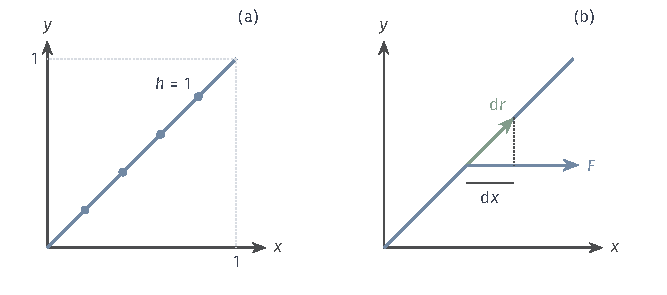
\includegraphics[width=112mm]{figures/00-shared/mathematical-preliminaries-upper/00-shared/tikz/chapter3-concept-processes/line-density-work.pdf}
 \caption{路径均为$\gamma(t)=(t,t)^\top$，$0\leq t\leq1$。(a) 常数线密度$h=1$按弧长累计，得到$\sqrt2$。(b) 常向量场$\bm F=(1,0)^\top$只取位移的水平分量，做功为$1$；图中$\mathrm dx$是$\mathrm d\bm r$的水平投影。相同路径、不同被积对象和权重给出不同积分。}
 \label{fig:analysis-process-line-density-work}
\end{figure}

\subsubsection{积分的基本性质}

下列公式均由内积的线性和一元Riemann积分的相应性质得到。以下说$\bm F$沿$\gamma$可积，是指沿各段满足前述连续性条件，因而相应的有向积分有限。前三条说明功对力是线性的，接下来三条说明功怎样随路径的拼接、方向和参数化变化，最后一条估计功的大小。

\paragraph{加法}

若$\bm F$和$\bm G$沿$\gamma$可积，则$\bm F+\bm G$也沿$\gamma$可积，且
\[
 \int_\gamma(\bm F+\bm G)\cdot\mathrm d\bm r
 =\int_\gamma\bm F\cdot\mathrm d\bm r+\int_\gamma\bm G\cdot\mathrm d\bm r.
\]
这里先把两个向量场相加，再与位移取内积。两个力同时作用时，合力做的功等于两个力各自做功之和。

\paragraph{减法}

把$\bm G$换成相反场$-\bm G$，由加法得到
\[
 \int_\gamma(\bm F-\bm G)\cdot\mathrm d\bm r
 =\int_\gamma\bm F\cdot\mathrm d\bm r-\int_\gamma\bm G\cdot\mathrm d\bm r.
\]
可积性保证两个积分都有限，所以可以相减。

\paragraph{数乘}

对实数$c$，有
\[
 \int_\gamma c\bm F\cdot\mathrm d\bm r
 =c\int_\gamma\bm F\cdot\mathrm d\bm r.
\]
力放大$c$倍，功也放大$c$倍；$c<0$时力反向，功变号。路径本身没有改变。

\paragraph{路径拼接}

若$\gamma_1$和$\gamma_2$首尾相接，则
\[
 \int_{\gamma_1*\gamma_2}\bm F\cdot\mathrm d\bm r
 =\int_{\gamma_1}\bm F\cdot\mathrm d\bm r
 +\int_{\gamma_2}\bm F\cdot\mathrm d\bm r.
\]
先走一段再走一段，总功是两段的功之和。因此分段光滑路径可以逐段计算，但每段都必须按这次行进的实际方向参数化。

\paragraph{方向反转}

记反向路径为$\gamma^{-}(u)=\gamma(a+b-u)$，$a\leq u\leq b$，它从$\gamma(b)$出发、沿原路走回$\gamma(a)$。由链式法则，它的速度是$-\gamma'(a+b-u)$，与原速度相反；再用一元换元$t=a+b-u$，得到
\[
 \int_{\gamma^{-}}\bm F\cdot\mathrm d\bm r
 =-\int_\gamma\bm F\cdot\mathrm d\bm r.
\]
顺风骑车时风做正功，沿原路逆风骑回来，风在每一段都做等量的负功。第一类积分反向后不变，因为长度始终非负；有向位移反向则改变符号。
特别地，往返路径$\gamma*\gamma^{-}$上的第二类积分为零，而它的长度是$\gamma$的两倍；示例~\ref{ex:analysis-diagonal-segment-paths}中的$\rho$就是对角线段上的这种往返路径。

\paragraph{重参数化}

若$t=\sigma(u)$为端点相配、严格递增的分段$C^1$微分同胚，则
$(\gamma\circ\sigma)'(u)=\gamma'(\sigma(u))\sigma'(u)$。在参数公式中应用换元$t=\sigma(u)$，得到
\[
 \int_{\gamma\circ\sigma}\bm F\cdot\mathrm d\bm r
 =\int_\gamma\bm F\cdot\mathrm d\bm r.
\]
也就是说，功只取决于经过哪些位置、朝哪个方向经过，与走得快慢无关。
与第一类积分不同，这里乘的是$\sigma'$本身而不是$|\sigma'|$。严格递减的重参数化把路径变成反向路径，换元后积分上下限交换，积分因此变号。重参数化也不改变经过的次数，同一段路重复走两次时，两次的功都会计入。

\paragraph{绝对值不等式}

由积分的三角不等式和Cauchy--Schwarz不等式$|\bm F^\top\bm\tau|\leq\lVert\bm F\rVert_2$可得
\[
 \left|\int_\gamma\bm F\cdot\mathrm d\bm r\right|
 \leq\int_\gamma\lVert\bm F\rVert_2\,\mathrm ds.
\]
功的绝对值不超过力的大小沿路程的累计；当力处处沿前进方向时取等号。若力的大小不超过$M$，路径长为$\ell$，功的绝对值便不超过$M\ell$。
本节的连续性条件保证右侧有限。

\subsubsection{积分的计算}

计算第二类路径积分时，按行进方向参数化路径，把场值与速度向量取内积，再做一元积分。与第一类积分相比，这里乘的是速度向量而不是速率。
先用图~\ref{fig:analysis-process-line-density-work}右图中的常力检验这一步骤。
\begin{example}[常力沿对角线段做功]
取常向量场$\bm F=(1,0)^\top$与对角线段$\gamma(t)=(t,t)^\top$，$0\leq t\leq1$。速度为$(1,1)^\top$，被积函数为$1\cdot1+0\cdot1=1$，所以
\[
 \int_\gamma\bm F\cdot\mathrm d\bm r=\int_0^1 1\,\mathrm dt=1.
\]
\end{example}
同一路径的长度为$\sqrt2$。功为$1$而不是$\sqrt2$，是因为水平方向的力只对位移的水平分量做功，而线段的水平跨度是$1$。

再看地面附近的重力。它同样是常向量场，这次让路径任意弯曲。
\begin{example}[重力做功只取决于高度差]
\label{ex:analysis-gravity-work}
设质量为$m$的物体沿分段$C^1$平面路径$\gamma(t)=(x(t),y(t))^\top$，$a\leq t\leq b$，从高度$y(a)$移动到高度$y(b)$，所受重力为$\bm F=(0,-mg)^\top$。被积函数为$\bm F(\gamma(t))^\top\gamma'(t)=-mg\,y'(t)$。在每个光滑段上用一元基本定理，再把各段相加，得到
\[
 \int_\gamma\bm F\cdot\mathrm d\bm r
 =\int_a^b(-mg)\,y'(t)\,\mathrm dt=-mg\bigl(y(b)-y(a)\bigr).
\]
例如质量为$1$千克的物体下降$2$米，即$y(b)-y(a)=-2$，取$g\approx9.8$米每二次方秒，无论沿斜坡还是沿弯曲的滑梯，重力都做功约$9.8\times2=19.6$焦。
\end{example}
被积函数中不含$x'(t)$，水平移动不受重力影响，只有高度变化起作用。这个结果只依赖起点和终点的高度，第~\ref{sec:multivariable-potential-path-independence}节将说明这并非偶然。

对平面图像路径$\gamma(x)=(x,\psi(x))^\top$、$a\leq x\leq b$，其中$\psi$为$C^1$，速度为$(1,\psi'(x))^\top$。$\bm F=(P,Q)^\top$时有
\[
 \int_\gamma\bm F\cdot\mathrm d\bm r
 =\int_a^b\bigl[P(x,\psi(x))+Q(x,\psi(x))\psi'(x)\bigr]\,\mathrm dx.
\]

重力的功与路线无关。下面固定起点和终点，比较两条路线上的功，观察一般向量场是否也如此。
\begin{example}[半圆和直径]
\label{ex:analysis-path-integral-comparison}
取上半圆$\gamma(t)=(\cos t,\sin t)^\top$，$0\leq t\leq\pi$，它从$(1,0)$逆时针走到$(-1,0)$，速度为$(-\sin t,\cos t)^\top$，速率为$1$，故长度$\int_\gamma1\,\mathrm ds=\pi$。另取起点和终点相同的直径$\lambda(t)=(1-2t,0)^\top$，$0\leq t\leq1$，速度为$(-2,0)^\top$。

对常场$(1,0)^\top$，沿上半圆的功为$\int_0^\pi(-\sin t)\,\mathrm dt=-2$，沿直径的功为$\int_0^1(-2)\,\mathrm dt=-2$。两条路线都向左净移动了$2$，水平向右的力在两条路线上做功都是$-2$，恰等于函数$\phi(x,y)=x$在终点与起点的差$-1-1$。

对旋转场$\bm F=(-y,x)^\top$，沿上半圆有$\bm F(\gamma(t))=(-\sin t,\cos t)^\top$，与速度相同，内积为$\sin^2t+\cos^2t=1$，故功为$\pi$：质点一直顺着旋转方向走。
沿直径，$\bm F(\lambda(t))=(0,1-2t)^\top$竖直，而位移水平，内积恒为零，功为$0$。
两条路线端点相同，旋转场做的功却不同。
\end{example}

对常场，功与路线无关；对旋转场，功依赖于路线。沿完整单位圆逆时针一周，质点回到起点，旋转场做功$2\pi$而不是零。图~\ref{fig:analysis-process-rotation-field-paths}画出了旋转场与这两条路线。
\begin{figure}[!htbp]
 \centering
 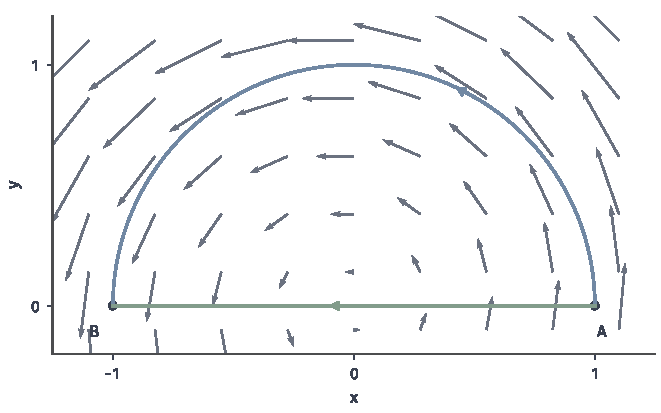
\includegraphics[width=112.0mm]{figures/00-shared/mathematical-preliminaries-upper/00-shared/matplotlib/chapter3-concept-processes/rotation-field-paths.pdf}
 \caption{灰箭头为旋转场$\bm F=(-y,x)^\top$，箭头长度统一缩放为实际场值的$1/4$。两条路径都从$A=(1,0)$到$B=(-1,0)$：蓝色上半圆与场同向，积分为$\pi$；绿色直径上场与位移垂直，积分为零。旋转场处处光滑，端点相同的两条路径上积分仍可不同；下一小节说明势函数给出的路径无关条件。}
 \label{fig:analysis-process-rotation-field-paths}
\end{figure}

\subsection{路径无关与势函数}
\label{sec:multivariable-potential-path-independence}

重力的功只依赖起点和终点的高度，旋转场的功却依赖路线。区别在于：重力的功可以写成某个只依赖位置的量在两端的差，这个量是$-mgy$；旋转场则没有这样的量。
本小节先说明这样的量，即势函数，如何把沿途累计化为端点差；再证明“功与路线无关”反过来也能构造出势函数；最后给出可以直接检查的微分条件，并说明定义域中有洞时，这个条件为什么不再足以保证势函数存在。

\subsubsection{势函数与路径积分}

\paragraph{势函数}

物理中，地面附近质量为$m$的物体在高度$y$处的重力势能为$E_{\mathrm p}(x,y)=mgy$。重力等于势能梯度的相反向量：$-\nabla E_{\mathrm p}=(0,-mg)^\top$。物体下降时势能减少，减少的势能等于重力做的功。
数学中习惯省去负号，取$\phi=-E_{\mathrm p}$，直接要求向量场等于某个标量函数的梯度。
\begin{definition}[势函数]
设$U\subseteq\mathbb R^d$为非空开集，$\bm F:U\to\mathbb R^d$连续。
若存在$\phi\in C^1(U)$使$\bm F=\nabla\phi$，称$\phi$为$\bm F$的\term{势函数}（potential function），称$\bm F$为梯度场，也称保守场。
\end{definition}

梯度指向函数增长最快的方向，所以在梯度非零处，梯度场的箭头指向$\phi$增大的方向，也就是势能$-\phi$减小的方向：重力把物体拉向低处。
例如$\phi(x,y)=x^2+y^2$给出$\bm F(x,y)=(2x,2y)^\top$，箭头从原点向外，因为离原点越远$\phi$越大；常场$(1,0)^\top$的一个势函数是$\phi(x,y)=x$。

给势函数加一个常数，梯度不变，所以势函数不唯一。若$U$还是路径连通的，两个势函数也只能相差一个常数：它们之差的梯度处处为零，路径连通的开集中任意两点都能用域内折线连接，沿折线逐段使用中值公式（定理~\ref{thm:multivariable-scalar-mean-value}），可知这个差在任意两点取值相同。
这与物理中势能的零点可以任选是同一件事：把地面还是桌面取作高度零点，算出的势能差都一样。

“保守”这个名称来自能量守恒。

设质量为$m$的质点在力场$\bm F=\nabla\phi$中按牛顿第二定律$m\gamma''(t)=\bm F(\gamma(t))$运动，其中$\gamma$为$C^2$路径。依次用乘积法则、运动方程和链式法则，得到
\[
 \frac{\mathrm d}{\mathrm dt}\Bigl(\tfrac12m\lVert\gamma'(t)\rVert_2^2\Bigr)
 =m\gamma''(t)^\top\gamma'(t)=\nabla\phi(\gamma(t))^\top\gamma'(t)
 =\frac{\mathrm d}{\mathrm dt}\phi(\gamma(t)),
\]
所以动能与势能$-\phi$之和$\frac12m\lVert\gamma'\rVert_2^2-\phi(\gamma)$的导数为零，不随时间变化。最后一个等号已经显示了下面定理的核心：沿路径的功率$\nabla\phi^\top\gamma'$恰是$\phi\circ\gamma$的导数。

\paragraph{路径积分基本定理}

一元基本定理说，导数在区间上的积分等于原函数在两端的差。把势函数与路径复合，得到一元函数$t\mapsto\phi(\gamma(t))$，它的导数恰是第二类路径积分的被积函数，因此一元基本定理直接给出端点差。
直观上，每一小段的功$\nabla\phi^\top\Delta\bm r$近似等于$\phi$在这一小段上的增量，这些增量相加时中间各项逐一抵消，只剩终点值减起点值。
\begin{theorem}[路径积分基本定理]
设$U\subseteq\mathbb R^d$为开集，$\phi\in C^1(U)$，$\gamma:[a,b]\to U$分段$C^1$。则
\begin{equation}
  \int_{\gamma}\nabla\phi\mathbin{\cdot}\mathrm{d}\bm{r}
  =\phi(\gamma(b))-\phi(\gamma(a)).
\label{eq:analysis-line-integral-gradient}
\end{equation}
\end{theorem}
\begin{proof}
在每个光滑参数段$[t_{j-1},t_j]$上，链式法则给出
\[
 (\phi\circ\gamma)'(t)=\nabla\phi(\gamma(t))^\top\gamma'(t).
\]
右侧是连续函数的复合与乘积，在该段上连续，所以对该段使用一元基本定理，得到
$\int_{t_{j-1}}^{t_j}\nabla\phi(\gamma(t))^\top\gamma'(t)\,\mathrm dt=\phi(\gamma(t_j))-\phi(\gamma(t_{j-1}))$。
对$j=1,\dots,n$相加，中间端点的值一正一负逐一抵消，只剩$\phi(\gamma(b))-\phi(\gamma(a))$。
\end{proof}

用势能$E_{\mathrm p}=-\phi$来读，式~\eqref{eq:analysis-line-integral-gradient}说：保守力沿任何路线做的功都等于起点势能减终点势能，即势能的下降量。示例~\ref{ex:analysis-gravity-work}的重力做功就是$\phi(x,y)=-mgy$的情形。

这个定理有两个直接推论。第一，梯度场的积分只依赖端点：两条端点相同的路线，功相同。第二，闭路径的起点与终点重合，所以梯度场沿任意闭路径的积分为零：把书从地上拿到桌上再放回地上，重力在全过程中做的总功为零。
方向反转时端点交换，端点差变号，这与第二类积分的方向反转性质一致。

知道势函数后，计算路径积分不必代入参数。
\begin{example}[用势函数计算沿半圆的积分]
取$\bm F=(2x,2y)^\top$，它的势函数为$\phi(x,y)=x^2+y^2$。路径取示例~\ref{ex:analysis-path-integral-comparison}中的上半圆$\gamma(t)=(\cos t,\sin t)^\top$，$0\leq t\leq\pi$，从$(1,0)$走到$(-1,0)$。由式~\eqref{eq:analysis-line-integral-gradient}，
\[
 \int_\gamma\bm F\cdot\mathrm d\bm r=\phi(-1,0)-\phi(1,0)=1-1=0.
\]
直接代入参数也得到同样结果：$\bm F(\gamma(t))^\top\gamma'(t)=2\cos t\,(-\sin t)+2\sin t\cos t=0$。这个场在圆周上处处沿半径方向，与切线垂直。
\end{example}

第二个推论还可以用来否定势函数的存在。旋转场沿单位圆逆时针一周做功$2\pi\neq0$，所以它在$\mathbb R^2$上没有势函数。

\subsubsection{路径无关的等价判别}

\paragraph{路径无关}

路径积分基本定理说明，有势函数就能推出功与路线无关。要讨论反方向，先把“与路线无关”说准确。比较同一对端点间的不同路线，需要域内任意两点都能用路径连接；对欧氏开集，路径连通时任意两点之间还能选到域内的折线，因而能选到分段光滑路径。
\begin{definition}[路径无关]
设$U\subseteq\mathbb R^d$为非空、开且路径连通的集合，$\bm F:U\to\mathbb R^d$连续。
若对任意$\bm a,\bm b\in U$及域内从$\bm a$到$\bm b$的任意两条分段$C^1$路径，第二类路径积分都相等，称$\bm F$的路径积分与路径无关。
\end{definition}

反方向的想法来自物理中定义势能的办法：选定一个参考点作为势能零点，把力从参考点到某点所做的功取负号，作为该点的势能。只有当这个功与所选路线无关时，这样定义的势能才是一个确定的数。下面的定理说明，路径无关、闭路径积分为零与势函数存在三者等价。
\begin{theorem}[路径无关的等价条件]
设$U\subseteq\mathbb R^d$非空、开且路径连通，$\bm F:U\to\mathbb R^d$连续。下列条件等价：
\begin{enumerate}
 \item 存在$\phi\in C^1(U)$使$\nabla\phi=\bm F$；
 \item $\bm F$的路径积分与路径无关；
 \item 域内每条分段$C^1$闭路径的积分都为零。
\end{enumerate}
\end{theorem}
\begin{proof}
条件1推出条件2，是路径积分基本定理的第一个推论。
条件2推出条件3：设$\gamma$是从$\bm a$出发回到$\bm a$的闭路径。停在$\bm a$不动的常值路径也从$\bm a$到$\bm a$，它的速度为零，积分为零；由路径无关，$\gamma$上的积分也为零。
条件3推出条件2：设$\gamma_1,\gamma_2$都从$\bm a$到$\bm b$。先沿$\gamma_1$走到$\bm b$，再沿$\gamma_2$的反向路径$\gamma_2^-$走回$\bm a$，拼成闭路径$\gamma_1*\gamma_2^-$。由拼接和方向反转性质，
\[
 0=\int_{\gamma_1*\gamma_2^-}\bm F\cdot\mathrm d\bm r
 =\int_{\gamma_1}\bm F\cdot\mathrm d\bm r-\int_{\gamma_2}\bm F\cdot\mathrm d\bm r.
\]

最后由条件2构造势函数。固定参考点$\bm a\in U$，对每个$\bm x\in U$，取域内任意一条从$\bm a$到$\bm x$的分段$C^1$路径，令$\phi(\bm x)$为沿它的积分。路径无关保证这个数不依赖所选路线。
下面计算偏导数。因为$U$开，存在$r>0$使以$\bm x$为中心、半径$r$的球在$U$内。对$0<|h|<r$，到$\bm x+h\bm e_j$的一条路径可以这样选：先沿原来的路径走到$\bm x$，再沿第$j$个坐标方向走线段$t\mapsto\bm x+t\bm e_j$，$t$从$0$到$h$。线段的速度为$\bm e_j$，场与速度的内积是第$j$个分量$F_j$，于是
\[
 \phi(\bm x+h\bm e_j)-\phi(\bm x)
 =\int_0^h F_j(\bm x+t\bm e_j)\,\mathrm dt.
\]
（$h<0$时按有向积分理解。）右侧除以$h$，是$F_j$在这条短线段上的平均值。$F_j$连续，$h\to0$时这个平均值趋于$F_j(\bm x)$，所以$\partial_j\phi(\bm x)=F_j(\bm x)$。
所有偏导数都等于$\bm F$的连续分量，故$\phi\in C^1(U)$且$\nabla\phi=\bm F$，得到条件1。
\end{proof}

证明中的$\phi$正是“从参考点出发做的功”。换一个参考点$\bm a'$，$\phi$只改变一个常数，即从$\bm a'$到$\bm a$的功，这与势能零点可以任选一致。

\subsubsection{势函数存在的微分判别}

\paragraph{交叉偏导相等的必要条件}

路径无关的等价条件把势函数的存在归结为检查所有路径或所有闭路径，实际上无法逐条验证。我们希望找到只需对$\bm F$求导就能检查的条件。
若$\bm F=\nabla\phi$，则$F_j=\partial_j\phi$。当$\bm F$本身是$C^1$时，$\phi$具有连续的二阶偏导数，由定理~\ref{thm:multivariable-mixed-partials}，混合偏导可以交换次序，于是$\bm F$的分量之间必须满足一组关系。
\begin{theorem}[保守场的必要条件]
设$U\subseteq\mathbb R^d$为开集，$\bm F\in C^1(U;\mathbb R^d)$。
若$\bm F=\nabla\phi$，其中$\phi\in C^1(U)$，则对所有$i,j$和$\bm x\in U$，有
\[
 \partial_iF_j(\bm x)=\partial_jF_i(\bm x).
\]
\end{theorem}
\begin{proof}
由$\partial_j\phi=F_j\in C^1(U)$可知$\phi\in C^2(U)$，因此
$\partial_iF_j=\partial_i\partial_j\phi=\partial_j\partial_i\phi=\partial_jF_i$。
\end{proof}

在平面中，记$\bm F=(P,Q)^\top$，条件只有一个：$\partial_xQ=\partial_yP$。差$\partial_xQ-\partial_yP$有清楚的几何含义：它度量向量场在一点附近的旋转程度。

为看出这一点，计算沿一个小正方形边界的环流。

设正方形为$[x_0,x_0+\delta]\times[y_0,y_0+\delta]$，按逆时针方向行走。下边向右，贡献$\int_{x_0}^{x_0+\delta}P(x,y_0)\,\mathrm dx$；上边向左，贡献$-\int_{x_0}^{x_0+\delta}P(x,y_0+\delta)\,\mathrm dx$。$P$在上下两边相差约$\partial_yP\,\delta$，所以这两项之和约为$-\partial_yP\cdot\delta\cdot\delta$。同理，右边向上、左边向下，两者的贡献之和约为$\partial_xQ\cdot\delta^2$。
因此小正方形的环流约为$(\partial_xQ-\partial_yP)\,\delta^2$，即单位面积上的环流约为$\partial_xQ-\partial_yP$，下面称它为旋转率。

保守场沿每条闭路径做功为零，小正方形也不例外，所以旋转率必须处处为零，这与上面的必要条件一致。这里只是近似推理；沿区域边界的环流与区域内旋转率的精确关系是Green公式，见定理~\ref{thm:multivariable-green}。

两个例子可以对照。场$(2x,2y)^\top$满足$\partial_xQ=0=\partial_yP$，它确实有势函数$x^2+y^2$。旋转场$(-y,x)^\top$有$\partial_xQ-\partial_yP=1-(-1)=2\neq0$，它在每一点附近都在旋转，由上面的必要条件，它在任何非空开集上都没有势函数。这与单位圆上环流为$2\pi$的计算一致：$2\pi$恰是旋转率$2$乘单位圆盘的面积$\pi$。

\paragraph{星形域上的充分条件}

交叉偏导相等只说明每个小区域内没有旋转，它是局部条件；势函数却要在整个定义域上用一个函数表示。要从局部条件得到全局结论，还需要对定义域本身加条件。

一个便于直接构造的条件是星形：若存在$\bm a\in U$，使从$\bm a$到每个$\bm x\in U$的整条线段都在$U$内，称$U$关于$\bm a$星形。凸开集满足这一条件，整个$\mathbb R^d$也满足。
在星形域上，可以沿用路径无关等价条件证明中“从参考点出发做功”的办法定义势函数，并且总沿直线段从$\bm a$走到$\bm x$。
\begin{theorem}[星形域上势函数的构造]
设$U\subseteq\mathbb R^d$为关于$\bm a$星形的开集，$\bm F\in C^1(U;\mathbb R^d)$，且对所有$i,j$有$\partial_iF_j=\partial_jF_i$。则
\[
 \phi(\bm x)=\int_0^1\bm F(\bm a+t(\bm x-\bm a))^\top(\bm x-\bm a)\,\mathrm dt
\]
属于$C^1(U)$且满足$\nabla\phi=\bm F$。因此$\bm F$的路径积分与路径无关。
\end{theorem}
\begin{proof}
记$\bm z=\bm x-\bm a$。$\phi(\bm x)$是$\bm F$沿线段$t\mapsto\bm a+t\bm z$，$0\leq t\leq1$，的第二类路径积分，因为这条线段的速度恒为$\bm z$。
固定$\bm x$时，这条线段是$U$内的紧集，因而它的一个足够小的紧邻域仍在$U$内；当$\bm x$在一个小范围内变动时，相应线段都留在这个紧邻域中。
$\bm F$及其一阶偏导在紧邻域上连续因而有界，所以被积函数对$x_j$的偏导数有不依赖$t$的上界，可以用式~\eqref{eq:classical-differentiate-under-integral}在积分号下对$x_j$求导。

被积函数为$\sum_iF_i(\bm a+t\bm z)z_i$。对$x_j$求导时，$z_j$对$x_j$的导数为$1$，$F_i(\bm a+t\bm z)$对$x_j$的导数由链式法则为$t\,\partial_jF_i(\bm a+t\bm z)$，所以偏导数为
\[
 F_j(\bm a+t\bm z)+t\sum_i z_i\partial_jF_i(\bm a+t\bm z).
\]
交叉偏导条件把$\partial_jF_i$换成$\partial_iF_j$，而$\sum_iz_i\partial_iF_j(\bm a+t\bm z)$正是$t\mapsto F_j(\bm a+t\bm z)$的导数，于是
\[
 \begin{aligned}
 F_j(\bm a+t\bm z)+t\sum_i z_i\partial_jF_i(\bm a+t\bm z)
 &=F_j(\bm a+t\bm z)+t\sum_i z_i\partial_iF_j(\bm a+t\bm z)\\
 &=\frac{\mathrm d}{\mathrm dt}\bigl[tF_j(\bm a+t\bm z)\bigr].
 \end{aligned}
\]
对$t$从$0$积分到$1$，由一元基本定理得$\partial_j\phi(\bm x)=1\cdot F_j(\bm a+\bm z)-0=F_j(\bm x)$。
这些偏导连续，所以$\phi\in C^1(U)$；路径无关由前一定理得到。
\end{proof}

用这个构造可以求出一个具体平面场的势函数。
\begin{example}[沿线段构造势函数$x^2y$]
取$\bm F(x,y)=(2xy,x^2)^\top$，即$P=2xy$，$Q=x^2$。它定义在整个平面上，分量都是多项式，属于$C^1$，并且$\partial_yP=2x=\partial_xQ$。整个平面关于$\bm a=\bm0$星形，代入构造公式，
\[
 \phi(x,y)=\int_0^1\bigl[2(tx)(ty)\,x+(tx)^2\,y\bigr]\,\mathrm dt
 =\int_0^13t^2x^2y\,\mathrm dt=x^2y.
\]
直接求导可验证$\nabla\phi=(2xy,x^2)^\top$。于是这个场沿任何从$(0,0)$到$(1,2)$的分段$C^1$路径做功都等于$\phi(1,2)-\phi(0,0)=2$。
\end{example}
星形域上的构造不依赖猜测：交叉偏导相等时，沿线段积分就给出势函数，任意路径上的功随之化为端点差。

\paragraph{穿孔平面上的反例}

星形域的条件不能省略。下面的向量场在原点以外处处满足交叉偏导条件，在穿孔平面上却没有势函数。
\begin{example}[穿孔平面上的涡旋场]
\label{ex:analysis-punctured-plane-vortex}
在穿孔平面$\mathbb R^2\setminus\{\bm0\}$上考虑
\[
 \bm F(x,y)=\left(-\frac{y}{x^2+y^2},\frac{x}{x^2+y^2}\right)^\top ,
\]
记它的两个分量为$P,Q$。它与旋转场$(-y,x)^\top$方向相同，都沿逆时针方向与以原点为圆心的圆相切，但大小改为到原点距离的倒数：离原点越近转得越快，类似于绕一根细涡管旋转的水流。原点处它没有定义。

先检查交叉偏导。由商的求导法则，
\[
 \begin{aligned}
 \partial_yP&=-\frac{(x^2+y^2)-y\cdot2y}{(x^2+y^2)^2}=\frac{y^2-x^2}{(x^2+y^2)^2},\\
 \partial_xQ&=\frac{(x^2+y^2)-x\cdot2x}{(x^2+y^2)^2}=\frac{y^2-x^2}{(x^2+y^2)^2},
 \end{aligned}
\]
两者在穿孔平面上处处相等，所以这个场在原点以外的每一点附近都没有旋转。

再沿单位圆$\gamma(t)=(\cos t,\sin t)^\top$，$0\leq t\leq2\pi$，逆时针走一周。在单位圆上$x^2+y^2=1$，$\bm F(\gamma(t))=(-\sin t,\cos t)^\top$与速度相同，内积为$1$，积分为$2\pi$。
闭路径积分不为零，由路径无关的等价条件，$\bm F$在穿孔平面上没有势函数。
\end{example}

交叉偏导相等这个局部条件，在这里没能给出全局的势函数。这与星形域上的定理并不矛盾：穿孔平面不是星形域，对任一点$\bm a\neq\bm0$，从$\bm a$到$-\bm a$的线段都经过原点。问题出在原点这个洞上，可以从两个角度理解。

第一，局部的势函数是极角。在不含原点的区域上，若能连续地选取点$(x,y)$的极角$\theta$，使$x=r\cos\theta$、$y=r\sin\theta$，其中$r=\sqrt{x^2+y^2}$，则直接求导可得$\nabla\theta=\bm F$。例如在右半平面$x>0$上取$\theta=\arctan(y/x)$，有$\partial_x\theta=-y/(x^2+y^2)$，$\partial_y\theta=x/(x^2+y^2)$。
在更大的区域，即去掉负半轴的平面$\mathbb R^2\setminus\{(x,0)^\top:x\leq0\}$上，取$\theta\in(-\pi,\pi)$，它连续且仍满足$\nabla\theta=\bm F$；这个区域关于$(1,0)$星形，与星形域上的定理一致。

但在整个穿孔平面上无法连续地选取极角：从$(1,0)$出发绕原点逆时针一周回到$(1,0)$，极角连续地增加了$2\pi$，起点和终点处的“势函数值”对不上。单位圆上的积分$2\pi$正是极角的这个增量。
具体地，从$(1,0)$到$(-1,0)$，沿上半圆极角从$0$增加到$\pi$，积分为$\pi$；沿下半圆$(\cos t,-\sin t)^\top$，$0\leq t\leq\pi$，极角从$0$减少到$-\pi$，积分为$-\pi$。两条路线的功相差$2\pi$，恰是绕原点一圈的积分。
不绕原点的闭路径则没有这个问题。例如以$(3,0)$为圆心、半径为$1$的圆整个落在右半平面中，那里$\theta$是势函数，沿它的积分为零。

第二，从小正方形的环流看。交叉偏导相等说明每个小正方形的环流近似为零。若一条闭路径围住的区域整个在定义域内，可以把这个区域划分成许多小正方形；相邻正方形的公共边被沿相反方向各走一次，贡献相互抵消，只剩外边界，于是外边界的环流也为零。这一推理的精确形式就是Green公式（定理~\ref{thm:multivariable-green}），它要求向量场在整个被围区域附近都有定义且连续可微。

单位圆围住的圆盘却包含原点，那里$\bm F$没有定义，无法这样填满。场在定义域内的旋转率处处为零；非零环流与被排除的原点有关。对夹在两条绕原点闭路径之间、不含原点的环形区域作同样的划分，可知两条路径上的环流相等；所以绕原点逆时针一周的简单闭路径，积分都是$2\pi$，而围住的区域不含原点的闭路径，积分为零。

相比之下，星形域上不会出现这样的洞：任何闭路径都可以沿线段向中心点$\bm a$连续收缩而不离开定义域。这从几何上解释了，为什么在星形域上交叉偏导条件已经足以保证势函数存在。

\FloatBarrier

\par\Needspace{10\baselineskip}
\section{曲面积分}
\label{sec:analysis-surface-integration}

路径积分沿一条细线累计：线密度乘弧长得到质量，力与位移的内积累加得到做功。
曲面积分把累计的范围从细线换成薄片，典型问题有两个。
第一个问题是求一张金属薄壳的质量：已知壳上每点每平方米有多少千克，把各小片的“面密度乘面积”加起来即可。
第二个问题是求单位时间内有多少水穿过一张渔网：水在各点有速度，只有垂直于网面的速度分量才把水送到网的另一侧。

两个问题的被积对象不同。
在第一个问题中，被积对象是曲面$S$上的标量函数$h:S\to\mathbb R$，它给出每单位面积的密度，乘面积后相加得到质量、电荷等总量。
在第二个问题中，被积对象是向量场$\bm F:S\to\mathbb R^3$，它在每点给出一个有大小和方向的量；要先取它垂直于曲面的分量，再乘面积相加，得到穿过曲面的\emph{通量}。

两类积分都需要知道曲面上一小片有多大，所以本节先用参数化求出面积元。
通量还需要规定“从哪一侧穿到哪一侧算正”，因此在定义第二类积分之前，还要讨论曲面的定向。
本节的参数积分都按有界Jordan区域上的Riemann积分理解；参数曲面、面积元和通量的标准构造可参考\scite{math-openstax-calculus3}。

\subsection{参数曲面与面积元}

平面区域的面积就是它的Jordan面积。
空间中的曲面一般是弯曲的，不能不经伸缩地摊平成平面区域，所以不能直接用参数域的面积计算它的面积。
处理地球表面时，人们用经度和纬度两个数确定地面上的一点，这就是一种参数化：用两个参数标记曲面上的点，把曲面上的累计转回二维参数域上计算。
代价是参数域中的面积一般不等于曲面上的实际面积。
经纬度网格上同样大小的格子，在赤道附近和两极附近对应的实际地面面积并不相同，因此每一点都要乘一个面积放大倍数来校正。
本小节先说明怎样的参数化才能描述一张面，再求出这个放大倍数，并证明由此得到的面积不依赖参数的选取。

\subsubsection{曲面的参数化}

\paragraph{正则曲面片}

曲面的参数化是一个向量值映射：输入两个实数$(u,v)$，输出空间中一点的三个坐标。
并不是每个这样的映射都描述一张面。
若改变两个参数时点只沿同一个方向移动，像集可能只是一条曲线；
若不同参数在一块正面积的范围内对应同一些点，按参数累计就会把这块面计算两次。
下面的定义用正则性和单次覆盖两个条件分别排除这两种情况。

\begin{definition}[正则参数曲面片]
\label{def:analysis-regular-surface-patch}
设$E\subseteq\mathbb R^2$是有界闭区域，$E=\overline{E^\circ}$，其边界$\partial E$可用总面积任意小的有限个矩形覆盖。
设$\bm r$在$E$的一个开邻域内是$C^1$映射，写成
\[
 \bm r(u,v)=(x(u,v),y(u,v),z(u,v))^\top\in\mathbb R^3.
\]
若不同参数只有在都属于$\partial E$时才允许表示同一点，
且两个偏导向量$\bm r_u,\bm r_v$在$E^\circ$上处处线性无关，则称$\bm r$为一个正则曲面片的参数化，曲面片记为$S=\bm r(E)$。
参数边界允许产生接缝或退化点；这些边界部分按零曲面面积处理。
\end{definition}

定义中的两个偏导向量有直接的几何含义。
固定$v$而只改变$u$，点$\bm r(u,v)$在曲面上画出一条参数曲线，它的速度向量是$\bm r_u$；
固定$u$而改变$v$得到另一条参数曲线，速度向量是$\bm r_v$。
这里$\bm r_u,\bm r_v$都是三维向量，分别由三个坐标函数对同一个参数求偏导得到，并非某个标量函数的两个偏导数。

两个向量线性无关，是指对任意实数$\alpha,\beta$，
$\alpha\bm r_u+\beta\bm r_v=\bm0$只有在$\alpha=\beta=0$时才成立。
几何上，这表示两个向量不共线，它们张成过该点的一个平面，即曲面的切平面。
若这个条件不成立，像集可能根本不是一张面。

\begin{example}[像集退化为线段的参数映射]
取$E=[0,1]^2$和$\bm r(u,v)=(u+v,0,0)^\top$。
两个偏导向量都等于$(1,0,0)^\top$，因而线性相关。
当$(u,v)$取遍$E$时，$u+v$取遍$[0,2]$，所以像集是$x$轴上的线段$\{(x,0,0)^\top:0\leq x\leq2\}$。
整个正方形被压到这条线段上，像集上没有两个不共线的切方向，也没有面积可言；这个映射不满足正则性条件。
\end{example}

正则性条件排除了这种压扁的映射。
单次覆盖条件处理另一种情况：像集确实是一张面，但被参数重复计数。

\begin{example}[圆柱面的单次覆盖与二重覆盖]
\label{ex:analysis-cylinder-double-cover}
高为$1$的单位圆柱面可以写成
\[
\begin{gathered}
\bm r(\theta,z)=(\cos\theta,\sin\theta,z)^\top\\
z\in[0,1].
\end{gathered}
\]
偏导向量$\bm r_\theta=(-\sin\theta,\cos\theta,0)^\top$与$\bm r_z=(0,0,1)^\top$处处线性无关，正则性没有问题，需要检查的只有覆盖次数。
若$\theta\in[0,2\pi]$，只有$\theta=0$与$\theta=2\pi$两条边界线表示同一条接缝，这是定义允许的。
若$\theta\in[0,4\pi]$，则对$0<\theta_0<2\pi$和$0<z<1$，点$\bm r(\theta_0,z)$同时由参数域内部的$(\theta_0,z)$和$(\theta_0+2\pi,z)$表示；
按参数累计会把整张柱面计入两次，因此这一参数域不符合定义。
\end{example}

所以不同参数表示同一点的情形只允许出现在参数边界上，形成接缝；参数域内部的点不能与任何其他参数点表示同一点。

本小节反复使用的例子是$\bm r(u,v)=(u,v,u+v)^\top$、$E=[0,1]^2$，下文称它为斜平面片。
它描述平面$z=x+y$上位于单位正方形上方的一块平行四边形，
两个切向量分别为$\bm r_u=(1,0,1)^\top$和$\bm r_v=(0,1,1)^\top$。
前两个坐标就是参数本身，所以不同参数给出不同点；两个切向量不共线，所以它满足正则曲面片的定义。

\paragraph{叉积}

要求曲面的面积，先看参数域中的一个小矩形$[u,u+\Delta u]\times[v,v+\Delta v]$被映成什么形状。
由$\bm r$的可微性，在$\Delta u,\Delta v$很小时有线性近似
\[
 \bm r(u+\Delta u,v+\Delta v)\approx\bm r(u,v)+\bm r_u\Delta u+\bm r_v\Delta v,
\]
其中$\bm r,\bm r_u,\bm r_v$都在$(u,v)$处取值。
于是小矩形的四个顶点近似映为
$\bm r$、$\bm r+\bm r_u\Delta u$、$\bm r+\bm r_v\Delta v$和$\bm r+\bm r_u\Delta u+\bm r_v\Delta v$，
它们正是以$\bm r_u\Delta u$和$\bm r_v\Delta v$为两边的平行四边形的顶点。
所以曲面上的小片近似是切平面内的一个小平行四边形，问题归结为：怎样由两条边向量求平行四边形的面积。

在平面上，两个边向量排成$2\times2$矩阵，其行列式的绝对值就是这个面积。
现在两条边是三维向量，排成的是$3\times2$矩阵，没有行列式可取。
三维空间中常用叉积同时记录这个面积和平行四边形所在平面的垂直方向。
对$\bm a,\bm b\in\mathbb R^3$，定义叉积
\[
 \bm a\times\bm b
 =(a_2b_3-a_3b_2,\ a_3b_1-a_1b_3,\ a_1b_2-a_2b_1)^\top.
\]
例如$(1,0,0)^\top\times(0,1,0)^\top=(0,0,1)^\top$：
$x$轴方向与$y$轴方向的单位向量张成面积为$1$的正方形，叉积是长度为$1$、沿$z$轴的向量。

后面的面积和法向计算要用到叉积的三条性质，下面逐一核对。
第一，叉积垂直于$\bm a$和$\bm b$。直接展开
\[
 \bm a^\top(\bm a\times\bm b)
 =a_1(a_2b_3-a_3b_2)+a_2(a_3b_1-a_1b_3)+a_3(a_1b_2-a_2b_1),
\]
右端六项两两抵消，结果为$0$；对$\bm b$同理。
垂直于同一平面的方向有相反的两个，叉积按右手规则选取其中之一：右手四指从$\bm a$弯向$\bm b$时，拇指指向$\bm a\times\bm b$。

第二，叉积的长度等于$\bm a,\bm b$张成的平行四边形的面积。
把两边按分量展开，可以验证Lagrange恒等式
\[
 \lVert\bm a\times\bm b\rVert_2^2
 =\lVert\bm a\rVert_2^2\lVert\bm b\rVert_2^2-(\bm a^\top\bm b)^2.
\]
记$\theta\in[0,\pi]$为两向量的夹角，则$\bm a^\top\bm b=\lVert\bm a\rVert_2\lVert\bm b\rVert_2\cos\theta$，
代入得$\lVert\bm a\times\bm b\rVert_2=\lVert\bm a\rVert_2\lVert\bm b\rVert_2\sin\theta$。
以$\bm a$为底边时，平行四边形的高是$\lVert\bm b\rVert_2\sin\theta$，所以叉积长度正是“底乘高”。
特别地，叉积为零当且仅当两向量线性相关，即平行四边形退化为线段或一点。

第三，叉积对每个因子都是线性的，交换两个因子的次序会变号：从定义式直接看出$\bm b\times\bm a=-\bm a\times\bm b$，特别地$\bm a\times\bm a=\bm0$。
这与右手规则一致：交换次序后四指的弯曲方向相反，拇指也随之反向。

把这些性质用到小平行四边形上。由线性，
$(\bm r_u\Delta u)\times(\bm r_v\Delta v)=(\bm r_u\times\bm r_v)\Delta u\Delta v$；
再由第二条性质，小曲面片的面积近似为
\[
 \lVert\bm r_u\times\bm r_v\rVert_2\,\Delta u\,\Delta v.
\]
因此$\lVert\bm r_u\times\bm r_v\rVert_2$就是参数化在该点的面积放大倍数：参数域中面积为$\Delta u\Delta v$的小块，
在曲面上变成面积约为这个倍数乘$\Delta u\Delta v$的小片。
同样由第二条性质，正则性条件“两个切向量线性无关”可以等价地写成$\bm r_u\times\bm r_v\ne\bm0$，即放大倍数处处为正。

平面情形可以用来核对这个倍数。若曲面就在平面$z=0$内，即$\bm r(u,v)=(x(u,v),y(u,v),0)^\top$，
则$\bm r_u\times\bm r_v=(0,0,x_uy_v-x_vy_u)^\top$，其长度正是映射$(u,v)\mapsto(x,y)$的Jacobian行列式的绝对值。
这与第~\ref{sec:classical-change-variables}节换元公式中的面积权重$|\det\bm J_T|$一致；叉积长度是这个权重在三维空间中的推广。

\subsubsection{曲面面积的表示}

\paragraph{面积元与面积}

把参数域分成许多小矩形，由小平行四边形的面积近似，每块在曲面上的像的面积约为放大倍数乘参数面积，曲面的总面积约为这些乘积之和。
小矩形越细，线性近似越准确，求和的极限就是放大倍数在参数域上的积分。

这里直接把这个积分取作曲面面积的定义，而不像弧长那样用内接折线长度的上确界来定义，因为曲面上的类似做法会失败。
在一段有限高的圆柱面上，可以构造顶点都在柱面上的三角形网格（称为Schwarz灯笼），
使网格越来越细，三角形与柱面的夹角却不趋于零，三角形总面积可以趋于无穷。
用切平面上的平行四边形近似则不会出现这种问题，因为每个小平行四边形都贴着切平面。

\begin{definition}[曲面面积]
\label{def:analysis-surface-area-measure}
在单次覆盖的正则曲面片上，令$J_S=\|\bm r_u\times\bm r_v\|_2$。定义面积为
\[
 \operatorname{area}(S)=\iint_E J_S(u,v)\,\mathrm du\,\mathrm dv.
\]
面积元记为$\mathrm dS=J_S(u,v)\,\mathrm du\,\mathrm dv$。
\end{definition}

$J_S$在紧参数域上连续，所以积分存在。有限分片曲面的面积逐片相加；各片只沿边界接合，接缝的参数原像须能被任意小总面积的有限盒覆盖，以免重复累计。

用这一定义计算斜平面片的面积，并用初等几何核对结果。

\begin{example}[斜平面片的面积]
\label{ex:analysis-tilted-plane-area}
对斜平面片$\bm r(u,v)=(u,v,u+v)^\top$、$E=[0,1]^2$，按叉积的定义计算
\[
 \begin{aligned}
 \bm r_u\times\bm r_v
 &=(1,0,1)^\top\times(0,1,1)^\top\\
 &=(0\cdot1-1\cdot1,\ 1\cdot0-1\cdot1,\ 1\cdot1-0\cdot0)^\top
 =(-1,-1,1)^\top,
 \end{aligned}
\]
故$J_S=\lVert(-1,-1,1)^\top\rVert_2=\sqrt3$处处成立，曲面面积为
\[
 \operatorname{area}(S)=\int_0^1\int_0^1\sqrt3\,\mathrm du\,\mathrm dv=\sqrt3.
\]
用初等几何核对：两条边$\bm r_u,\bm r_v$的长度都是$\sqrt2$，内积为$1$，夹角余弦为$1/2$，即夹角为$60^\circ$；
平行四边形面积为$\sqrt2\cdot\sqrt2\cdot\sin60^\circ=\sqrt3$，与积分结果相同。
\end{example}

参数正方形的面积只有$1$，曲面片的面积却是$\sqrt3$：每个参数小块都被放大$\sqrt3$倍。
图~\ref{fig:analysis-process-surface-area-stretch}将参数小块与实际斜面小块对应起来，显示叉积长度校正的是哪一个面积。
\begin{figure*}[!htbp]
 \centering
 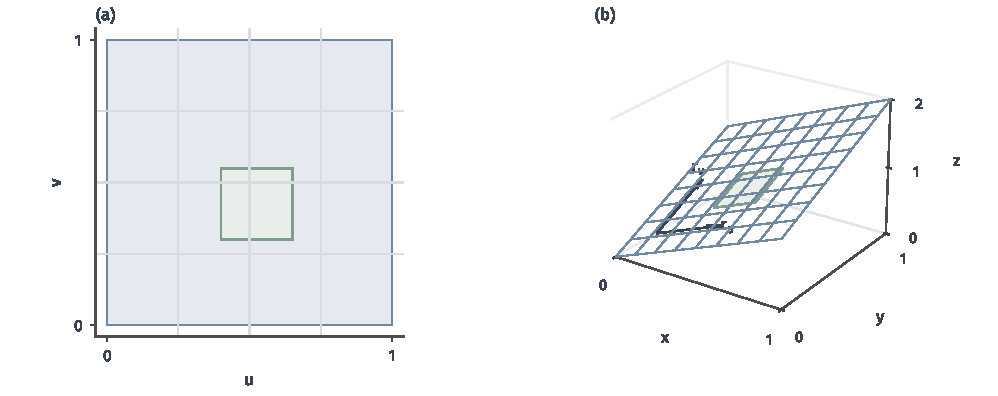
\includegraphics[width=169.0mm]{figures/00-shared/mathematical-preliminaries-upper/00-shared/matplotlib/chapter3-concept-processes/surface-area-stretch.pdf}
 \caption{参数化$r(u,v)=(u,v,u+v)^\top$把单位正方形映为斜平面片，绿色块为同一参数子区间及其像。两切向量$r_u=(1,0,1)^\top$、$r_v=(0,1,1)^\top$在右侧按$0.4$倍画出，叉积长度为$\sqrt3$。每个参数面积都放大$\sqrt3$倍，故不能把$\mathrm du\,\mathrm dv$直接当成$\mathrm dS$。}
 \label{fig:analysis-process-surface-area-stretch}
\end{figure*}

\paragraph{重参数化}

同一张面可以用不同参数标记。
面积是曲面本身的属性，不应随标记方式改变；先在斜平面片上核对一次具体的换参数。

\begin{example}[拉伸一个参数不改变面积]
\label{ex:analysis-stretched-parameter-area}
在斜平面片中令$u=2\xi$，则
\[
\begin{gathered}
\widetilde{\bm r}(\xi,v)=(2\xi,v,2\xi+v)^\top\\
(\xi,v)\in[0,1/2]\times[0,1]
\end{gathered}
\]
描述同一块平行四边形，新参数域的面积只有$1/2$。
另一方面，$\widetilde{\bm r}_\xi=(2,0,2)^\top=2\bm r_u$，$\widetilde{\bm r}_v=\bm r_v$，由叉积的线性，
$\widetilde{\bm r}_\xi\times\widetilde{\bm r}_v=2(\bm r_u\times\bm r_v)=2(-1,-1,1)^\top$，放大倍数为$2\sqrt3$。
因此
\[
 \int_0^1\int_0^{1/2}2\sqrt3\,\mathrm d\xi\,\mathrm dv=\sqrt3,
\]
与示例~\ref{ex:analysis-tilted-plane-area}的结果相同。
\end{example}

参数域缩小一半，每点的放大倍数恰好加倍，两者相互抵消。
下面的定理说明，这种抵消对一般的单次覆盖换参数都成立。

\begin{theorem}[重参数化下的面积元]
\label{thm:analysis-surface-reparameterization}
设$\bm r:E\to S$是正则曲面片的参数化，$T:\widetilde E\to E$是参数域之间的双射，
在$\widetilde E$的一个开邻域内为$C^1$映射，并且限制在$\widetilde E^\circ$上是到$E^\circ$的$C^1$微分同胚。
若$\widetilde{\bm r}=\bm r\circ T$仍满足曲面片条件，则
\[
 \begin{aligned}
 \widetilde{\bm r}_\xi\times\widetilde{\bm r}_\eta
 &=\det\bm J_T\,(\bm r_u\times\bm r_v)\circ T,\\
 \widetilde J_S&=(J_S\circ T)|\det\bm J_T|.
 \end{aligned}
\]
两组参数由此给出同一面积。
\end{theorem}

\begin{proof}
记$T(\xi,\eta)=(u(\xi,\eta),v(\xi,\eta))$。
链式法则给出$\widetilde{\bm r}_\xi=\bm r_u u_\xi+\bm r_v v_\xi$和
$\widetilde{\bm r}_\eta=\bm r_u u_\eta+\bm r_v v_\eta$，其中右端各量在$T(\xi,\eta)$处取值。
用叉积对每个因子的线性展开，得到四项：
\[
 \begin{aligned}
 \widetilde{\bm r}_\xi\times\widetilde{\bm r}_\eta
 &=u_\xi u_\eta(\bm r_u\times\bm r_u)+u_\xi v_\eta(\bm r_u\times\bm r_v)\\
 &\quad{}+v_\xi u_\eta(\bm r_v\times\bm r_u)\\
 &\quad{}+v_\xi v_\eta(\bm r_v\times\bm r_v).
 \end{aligned}
\]
由$\bm a\times\bm a=\bm0$，第一、四项为零；交换叉积次序会变号，即$\bm r_v\times\bm r_u=-\bm r_u\times\bm r_v$，于是第三项可与第二项合并。因此
\[
 \widetilde{\bm r}_\xi\times\widetilde{\bm r}_\eta
 =(u_\xi v_\eta-v_\xi u_\eta)(\bm r_u\times\bm r_v)\circ T,
\]
括号内正是$\det\bm J_T$，这就是第一式；两边取长度得到第二式。
把第二式在新参数域上积分，并应用经典二维换元公式，得到
\[
 \iint_{\widetilde E}(J_S\circ T)|\det DT|
 =\iint_E J_S.
\]
若换元只在参数域内部正则，先在远离边界的紧子域上应用公式，再利用连续有界权重和Jordan边界条件取极限。两组参数因而给出相同面积。
\end{proof}

几何上，这个证明把两步面积放大接在一起：新参数的小方块先由$T$映成原参数域中面积约为$|\det\bm J_T|$倍的小块，
这个小块再由$\bm r$映到曲面，面积又乘$J_S$。
二维换元公式恰好把第一步的倍数吸收掉，所以只剩下曲面本身的面积。
在示例~\ref{ex:analysis-stretched-parameter-area}中，$T(\xi,v)=(2\xi,v)$，$\det\bm J_T=2$，这正是放大倍数加倍的来源。

行列式的绝对值保证面积非负；行列式本身的符号则记录参数次序是否翻转。
例如在斜平面片上交换两个参数，令$T(\xi,\eta)=(\eta,\xi)$，即$\widetilde{\bm r}(\xi,\eta)=\bm r(\eta,\xi)=(\eta,\xi,\xi+\eta)^\top$，则$\det\bm J_T=-1$，
叉积由$(-1,-1,1)^\top$变为$(1,1,-1)^\top$，长度不变而方向相反。
面积不使用这个方向，后面选取通量的法向时则要用到它。

定理还要求$T$是双射。若参数在正面积的范围内重复覆盖，参数积分就会重复累计。
示例~\ref{ex:analysis-cylinder-double-cover}中，$\bm r_\theta\times\bm r_z=(\cos\theta,\sin\theta,0)^\top$，$J_S=1$；
$\theta\in[0,2\pi]$时参数积分给出柱面面积$2\pi$，$\theta\in[0,4\pi]$时却给出$4\pi$，不能当作单次覆盖的曲面面积。

\paragraph{分片曲面}

有些曲面不能用一张正则曲面片描述。单位立方体的表面由六个正方形组成，棱上没有切平面。
球面虽然可以用一张球坐标参数片覆盖（两极位于参数边界上，切向量在那里退化），也常分成上下两个半球分别处理。
本节只处理有限分片的情形：把曲面写成有限张正则曲面片的并，各片内部不重叠，交接部分在相邻曲面片中面积均为零，
整个曲面的面积由各片的面积相加。

例如立方体表面的面积就是六个单位正方形的面积之和$6$，十二条棱的面积为零，不需要在接缝上另加一项。
后面的两类曲面积分同样可以逐片计算再相加。
无界曲面，或不能这样由有限张正则曲面片覆盖的曲面，还需另外处理覆盖和可积性条件。

\subsection{第一类曲面积分}

有了面积，就可以回到本节开头的第一个问题：在曲面上累计一个标量密度。
这类积分只用到小片的面积，不涉及方向。

\subsubsection{积分的定义和可积性}

\paragraph{按面积的积分}

设一张薄金属壳占据曲面$S$，在点$\bm x$附近每单位面积的质量为$h(\bm x)$（单位如千克每平方米）。
把壳分成许多小片$S_j$，在每片内取一点$\bm x_j$。
若每片很小，片内面密度近似为常数$h(\bm x_j)$，这一片的质量约为$h(\bm x_j)\,\operatorname{area}(S_j)$。
把各片质量相加，再让分割越来越细，就得到面密度对面积的积分。
带电薄壳上的电荷量、涂层表面的涂料用量都是同一种累计。
下面将连续密度与面积权重相乘，再在参数域上积分。

\begin{definition}[第一类曲面积分]
\label{def:analysis-scalar-surface-integral}
设$h$是$S$上的连续标量函数，定义它的\term{第一类曲面积分}（scalar surface integral）为
\begin{equation}
 \int_Sh\,\mathrm dS
 =\iint_Eh(\bm r(u,v))J_S(u,v)\,\mathrm du\,\mathrm dv.
 \label{eq:analysis-scalar-surface-integral}
\end{equation}
右侧被积函数连续，因而积分存在且有限。
\end{definition}

式~\eqref{eq:analysis-scalar-surface-integral}右端的计算顺序是：用参数找到曲面上的点，读出该点的密度，乘该点的面积放大倍数，再在参数域上积分。
对定理~\ref{thm:analysis-surface-reparameterization}中的重参数化，把$h\circ\bm r$一并代入换元公式，可见积分值不变。
取$h=1$得到面积，取非负面密度得到质量。
例如在斜平面片上，常数密度$h=2$给出
\[
 \int_S2\,\mathrm dS=\int_0^1\int_0^1 2\sqrt3\,\mathrm du\,\mathrm dv=2\sqrt3,
\]
即面积为$\sqrt3$、每单位面积重$2$的薄片，总质量为$2\sqrt3$。

除了总量，第一类积分还给出曲面上的平均值。

设$0<\operatorname{area}(S)<\infty$且$h$曲面可积，则
\[
 \frac1{\operatorname{area}(S)}\int_Sh\,\mathrm dS
\]
是$h$按面积加权的平均。若$h$表示地球表面各点的气温，这个量就是全球表面平均气温：
每块地面按其实际面积参与平均，而不是按经纬度网格的格子数参与平均。

质量和平均值都只依赖每小片的大小，不依赖从哪一侧看曲面，所以把曲面的朝向反过来，第一类积分不变。

积分继承参数区域积分的线性、单调性和绝对值估计。有限分片上逐片求和，公共接缝不另计面积。特别地，连续密度满足
\[
 \left|\int_S h\,\mathrm dS\right|\leq\sup_S|h|\operatorname{area}(S).
\]
这些性质只依赖面积权重非负，因此改变曲面法向不会改变第一类积分。

\subsubsection{积分的计算}

计算第一类曲面积分分三步：选一个单次覆盖的正则参数化，把$h$与参数化复合，再乘叉积的长度后在参数域上积分。
最常见的两种参数化是函数图像和球坐标。

若曲面是函数$z=\psi(x,y)$在区域$D$上的图像，其中$D$满足定义~\ref{def:analysis-regular-surface-patch}对参数域的要求，$\psi$在$D$的开邻域内为$C^1$，就可以取
$\bm r(x,y)=(x,y,\psi(x,y))^\top$。此时$\bm r_x=(1,0,\psi_x)^\top$、$\bm r_y=(0,1,\psi_y)^\top$，按叉积公式计算得
\[
 \begin{aligned}
 \bm r_x\times\bm r_y
 &=(0\cdot\psi_y-\psi_x\cdot1,\ \psi_x\cdot0-1\cdot\psi_y,\ 1\cdot1-0\cdot0)^\top\\
 &=(-\psi_x,-\psi_y,1)^\top.
 \end{aligned}
\]
叉积的第三分量恒为$1$，所以图像参数化处处正则；前两个坐标就是参数本身，所以单次覆盖也自动成立。
于是对曲面可积的$h$有
\[
 \int_Sh\,\mathrm dS
 =\iint_Dh(x,y,\psi(x,y))\sqrt{1+\psi_x^2+\psi_y^2}\,\mathrm dx\,\mathrm dy.
\]

根号的几何意义如下。记$\gamma$为法向$(-\psi_x,-\psi_y,1)^\top$与$z$轴的夹角，
则$\cos\gamma=1/\sqrt{1+\psi_x^2+\psi_y^2}$。
一块与水平面成角$\gamma$的小平面片，竖直投影到$xy$平面上时面积缩小为原来的$\cos\gamma$倍；
反过来，由投影面积$\mathrm dx\,\mathrm dy$恢复实际面积，就要除以$\cos\gamma$，即乘上这个根号。
曲面越陡，根号越大。例如$z=ax+by+c$在单位圆盘上方的部分，根号处处等于$\sqrt{1+a^2+b^2}$，面积为
$\pi\sqrt{1+a^2+b^2}$；$a=b=0$时它就是水平圆盘的面积$\pi$。
若曲面不能单值地投影到同一坐标平面，例如整张球面在每个$(x,y)$上方有两点，则需换参数化或分片。

半径$R>0$的球面可以取参数
\[
 \begin{gathered}
 \bm r(\varphi,\theta)
 =(R\sin\varphi\cos\theta,R\sin\varphi\sin\theta,R\cos\varphi)^\top,\\
 0\leq\varphi\leq\pi,\quad 0\leq\theta\leq2\pi,
 \end{gathered}
\]
其中$\varphi$是与北极方向的夹角，$\theta$是绕$z$轴转过的角度。求偏导得
\[
 \begin{aligned}
 \bm r_\varphi&=(R\cos\varphi\cos\theta,R\cos\varphi\sin\theta,-R\sin\varphi)^\top,\\
 \bm r_\theta&=(-R\sin\varphi\sin\theta,R\sin\varphi\cos\theta,0)^\top.
 \end{aligned}
\]
这两个向量的内积为零，长度分别为$R$和$R\sin\varphi$；由叉积长度公式（夹角为$\pi/2$），叉积长度为$R^2\sin\varphi$。
这个结果也可以直接看出：$\varphi$增加$\Delta\varphi$时，点沿经线走过约$R\Delta\varphi$；
$\theta$增加$\Delta\theta$时，点沿半径为$R\sin\varphi$的纬线圈走过约$R\sin\varphi\,\Delta\theta$。
小片近似为以这两个长度为边的矩形。靠近两极时纬线圈变小，同样的$\Delta\theta$对应的面积也变小。

在参数域内部$0<\varphi<\pi$、$0<\theta<2\pi$上$\sin\varphi>0$，参数化正则且单次覆盖；
两极与经线接缝来自参数边界，面积为零，不需要单独处理。
先用这个参数化求球面面积。

\begin{example}[球面的面积]
\label{ex:analysis-sphere-area}
对半径为$R$的球面，球坐标参数的面积放大倍数为$J_S=R^2\sin\varphi$，被积函数连续，可以逐次积分：
\[
 \operatorname{area}(S)
 =\int_0^{2\pi}\int_0^\pi R^2\sin\varphi\,\mathrm d\varphi\,\mathrm d\theta
 =2\pi R^2\bigl[-\cos\varphi\bigr]_0^\pi
 =4\pi R^2.
\]
\end{example}





面积权重在求平均时同样不可缺少，下面以上半球面上的平均高度为例。

\begin{example}[上半球面的平均高度]
\label{ex:analysis-hemisphere-average-height}
取上半球面$0\leq\varphi\leq\pi/2$，高度函数$h(\bm x)=z$。
由$J_S=R^2\sin\varphi$，上半球面面积为$2\pi R^2\int_0^{\pi/2}\sin\varphi\,\mathrm d\varphi=2\pi R^2$，而
\[
 \int_Sz\,\mathrm dS
 =\int_0^{2\pi}\int_0^{\pi/2}R\cos\varphi\cdot R^2\sin\varphi\,\mathrm d\varphi\,\mathrm d\theta
 =2\pi R^3\cdot\frac12=\pi R^3,
\]
所以按面积加权的平均高度为$\pi R^3/(2\pi R^2)=R/2$。
若改为在参数矩形$[0,\pi/2]\times[0,2\pi]$上按参数面积平均，则得到
\[
 \frac1{(\pi/2)\cdot2\pi}\int_0^{2\pi}\int_0^{\pi/2}R\cos\varphi\,\mathrm d\varphi\,\mathrm d\theta
 =\frac{2R}{\pi}\approx0.64R.
\]
\end{example}

两种平均不同，是因为同样大小的参数格子在北极附近只对应很小的面积：按参数平均会过多计入北极附近的高点，因而高估平均高度。
面积权重$R^2\sin\varphi$正是为了按实际面积而不是按参数格子求平均。

\subsection{定向曲面与第二类曲面积分}

现在回到本节开头的第二个问题：向量场穿过曲面的总量。
面积只给出小片的大小；要说“穿过”，还必须先规定曲面的哪一侧算出发侧、哪一侧算到达侧。
因此本小节先讨论曲面的定向，再定义通量。

\subsubsection{曲面的定向}

\paragraph{单位法向量}

在正则点，切平面有两个互相相反的单位法向量，分别指向曲面的两侧。
选定其中一个，就约定：从曲面上背向它的一侧穿到它所指的一侧，算作正向穿越。
参数化的叉积给出一个自然的局部选择：在$E^\circ$上令
\[
 \bm n(\bm r(u,v))
 =\frac{\bm r_u\times\bm r_v}{\lVert\bm r_u\times\bm r_v\rVert_2}.
\]
由叉积的性质，这个向量长度为$1$，并且垂直于两个参数方向，即垂直于切平面；交换$u,v$的次序会把它反转。

在斜平面片上，这个公式给出$(-1,-1,1)^\top/\sqrt3$，它的第三分量为正，指向平面的上方。
在球坐标参数下，直接计算可得
\[
 \bm r_\varphi\times\bm r_\theta
 =R^2\sin\varphi\,(\sin\varphi\cos\theta,\sin\varphi\sin\theta,\cos\varphi)^\top
 =R\sin\varphi\,\bm r(\varphi,\theta).
\]
在参数域内部，叉积是位置向量的正数倍，所以单位法向为$\bm r/R$，指向球的外侧。
参数边界上若叉积退化，例如球面的两极，就不用这个商定义法向；该部分面积为零，不影响通量积分。

\paragraph{定向与可定向性}

只在每一点分别选一个法向还不够。若相邻两点选的法向分别指向曲面的两侧，“正向穿越”就没有一致的含义。
直观地说，给曲面定向就是给它的一侧涂上颜色，并约定法向总是从未涂色的一侧指向涂了色的一侧；
沿曲面连续移动时，法向箭头不能突然跳到另一侧。

\begin{definition}[曲面的定向]
\label{def:analysis-surface-orientation}
在光滑曲面$S$上连续选取一个单位法向量场$\bm n$，称为给曲面\term{定向}（orientation）。
存在这种选择的曲面称为可定向曲面；$\bm n$和$-\bm n$给出相反的定向。
分片光滑曲面要求各片的选择相容：光滑接合处选择同一侧法向，
折角处按整个曲面的同一侧约定，但不要求接缝上存在唯一法向。
\end{definition}

常见曲面都可以定向。函数图像可以选第三分量为正的向上法向；
球面可以选外法向$\bm x/R$，此时涂色的一侧是外表面。
闭曲面把空间分成内外两部分；当它围成一个规则区域时，通常选取指向区域外侧的外法向，第~\ref{sec:multivariable-boundary-relations}节的散度定理也采用这一约定。
立方体表面是分片曲面，六个面各自选指向立方体外的法向，这些选择在棱处都属于外侧，因而相容。

并非所有曲面都能定向，典型例子是Möbius带。把一条长纸带扭转半圈后，两端粘在一起，就得到这种曲面。
设想一只蚂蚁从某点出发，沿纸带中线爬一圈，始终不跨过纸带边缘；回到出发位置时，它却站在出发时的背面。
若想只涂纸带的一面，沿中线一直涂下去，最后整条纸带的两面都会被涂上颜色。
用参数可以把这一现象写成具体计算。

\begin{example}[Möbius带上的法向绕行一圈后反向]
\label{ex:analysis-mobius-normal-reversal}
取
\[
 \begin{gathered}
 \bm r(u,v)=\bigl(\lambda\cos u,\ \lambda\sin u,\ \tfrac v2\sin\tfrac u2\bigr)^\top,
 \qquad \lambda=1+\tfrac v2\cos\tfrac u2,\\
 0\leq u\leq2\pi,\quad -1\leq v\leq1.
 \end{gathered}
\]
$u$绕中心圆走一圈，$v$在纸带的宽度方向变化；绕行一圈时宽度方向只转过半圈，所以$\bm r(2\pi,v)=\bm r(0,-v)$，参数边界$u=0$与$u=2\pi$被反向粘在一起。
在中线$v=0$上，$\bm r_u=(-\sin u,\cos u,0)^\top$，$\bm r_v=\tfrac12\bigl(\cos\tfrac u2\cos u,\ \cos\tfrac u2\sin u,\ \sin\tfrac u2\bigr)^\top$，于是
\[
 \bm N(u)=\bm r_u\times\bm r_v=\tfrac12\bigl(\cos u\sin\tfrac u2,\ \sin u\sin\tfrac u2,\ -\cos\tfrac u2\bigr)^\top,
\]
它的长度恒为$1/2$。
$u=0$时它是$\frac12(0,0,-1)^\top$，$u=2\pi$时它是$\frac12(0,0,1)^\top$，而两者对应同一点$\bm r(0,0)=\bm r(2\pi,0)=(1,0,0)^\top$。

假设$\bm n$是Möbius带上连续的单位法向场。
在中线上的点$\bm r(u,0)$处，$\bm n$与$2\bm N(u)$都是单位法向，只能相等或相反。记
\[
 \varepsilon(u)=2\bm n(\bm r(u,0))^\top\bm N(u)\in\{1,-1\}.
\]
$\varepsilon$在$[0,2\pi]$上连续且只取$\pm1$，所以是常数。
但$\bm n(\bm r(0,0))=\bm n(\bm r(2\pi,0))$而$\bm N(2\pi)=-\bm N(0)$，从而$\varepsilon(2\pi)=-\varepsilon(0)$，矛盾。
因此Möbius带上不存在连续的单位法向场。
\end{example}

Möbius带的面积仍可按面积计算，第一类积分也有定义，因为它们不使用法向。
但“水从哪一侧流到哪一侧”在Möbius带上没有全局一致的含义，所以这里按全局定向定义的通量不适用于它。

\subsubsection{积分的定义和可积性}

\paragraph{通量积分}

先看最简单的情形。

设水以恒定速度$\bm v$流动，一块面积为$A$的平面网放在水中，选定单位法向$\bm n$。
在时间$\Delta t$内，恰好贴在网面上的水滴各自移动$\bm v\Delta t$，这段时间内穿过网的水因此充满一个斜柱体：
底面就是这块网，侧棱是向量$\bm v\Delta t$。
斜柱体的体积等于底面积乘高，高是侧棱在$\bm n$方向上投影的长度$|\bm v^\top\bm n|\Delta t$。
给这个体积加上符号，沿$\bm n$方向穿过记为正，就得到单位时间内沿$\bm n$方向穿过网的水量
\[
 \frac{A\,(\bm v^\top\bm n)\Delta t}{\Delta t}=(\bm v^\top\bm n)\,A.
\]

这个公式区分了三种情形。
若水流平行于网面，$\bm v^\top\bm n=0$，斜柱体被压扁成没有体积的薄片：水沿着网面滑过，没有水穿过网。
若水流沿$\bm n$方向垂直于网面，$\bm v^\top\bm n=\lVert\bm v\rVert_2$，同样流速下穿过的水最多。
若水逆着$\bm n$流动，$\bm v^\top\bm n<0$，结果为负，表示水沿$-\bm n$方向穿过；把法向换成$-\bm n$，同一股水流的结果就变号。
总之只有速度的法向分量$\bm v^\top\bm n$起作用，切向分量对穿过的水量没有贡献。

下面用一块倾斜的正方形核对这个公式，并比较竖直流与沿着正方形的流。

\begin{example}[竖直流与切向流穿过倾斜正方形]
\label{ex:analysis-tilted-square-flux}
设$0\leq\alpha\leq\pi/2$，倾斜的单位正方形为
\[
\begin{gathered}
\bm r(u,v)=(u\cos\alpha,\ v,\ u\sin\alpha)^\top\\
(u,v)\in[0,1]^2,
\end{gathered}
\]
它与水平面的夹角为$\alpha$。
由$\bm r_u=(\cos\alpha,0,\sin\alpha)^\top$和$\bm r_v=(0,1,0)^\top$，计算得$\bm r_u\times\bm r_v=(-\sin\alpha,0,\cos\alpha)^\top$。
它的长度为$1$，所以这块面的面积为$1$，单位法向为$\bm n=(-\sin\alpha,0,\cos\alpha)^\top$，其第三分量非负。
对竖直向上的恒定流$\bm F=(0,0,c)^\top$，$\bm F^\top\bm n=c\cos\alpha$，按平面网的公式，通量为$(\bm F^\top\bm n)\cdot1=c\cos\alpha$。
取$c=2$、$\alpha=60^\circ$，通量为$1$，只有水平放置（$\alpha=0$）时通量$2$的一半。
若改取沿正方形本身方向的流$\bm F=(\cos\alpha,0,\sin\alpha)^\top=\bm r_u$，
则$\bm F^\top\bm n=-\sin\alpha\cos\alpha+\sin\alpha\cos\alpha=0$，通量为零。
\end{example}

竖直流的通量$c\cos\alpha$也等于流速$c$乘这块面在水平面上的投影面积：正方形投影为矩形$[0,\cos\alpha]\times[0,1]$，面积为$\cos\alpha$。
这就是说，竖直落下的雨水，倾斜屋顶接到的雨量只取决于屋顶的水平投影。
切向流的结果则说明，沿曲面流动的场不穿过曲面。

对弯曲的曲面和随位置变化的场，把曲面分成小片$S_j$，在片内取点$\bm x_j$。
每片近似为平面，场在片内近似为常向量$\bm F(\bm x_j)$，所以由平面网的公式，这一片的通量约为$\bm F(\bm x_j)^\top\bm n(\bm x_j)\,\operatorname{area}(S_j)$。
各片相加并让分割变细，得到标量函数$\bm F^\top\bm n$对面积的积分。
$\bm F$不必是流速：电场的通量、热流密度的通量都按同样方式定义，分别描述电场穿过曲面的通量与单位时间穿过的热量。

\begin{definition}[第二类曲面积分]
\label{def:analysis-surface-flux-integral}
设可定向曲面$S$已选定单位法向$\bm n$，向量场$\bm F:S\to\mathbb R^3$连续。
定义\term{第二类曲面积分}（flux integral），也称通量积分，为
\begin{equation}
 \int_S\bm F^\top\bm n\,\mathrm dS
 =\iint_E\bm F(\bm r(u,v))^\top(\bm r_u\times\bm r_v)\,\mathrm du\,\mathrm dv,
 \label{eq:analysis-surface-flux}
\end{equation}
其中参数化的叉积方向须与所选$\bm n$一致；若方向相反，右端需乘$-1$。
分片曲面的通量按相容定向逐片相加。
\end{definition}

式~\eqref{eq:analysis-surface-flux}右端没有出现叉积的长度，因为单位法向的分母与面积元中的长度恰好抵消：
\[
 \bm n\,\mathrm dS
 =\frac{\bm r_u\times\bm r_v}{\lVert\bm r_u\times\bm r_v\rVert_2}\,\lVert\bm r_u\times\bm r_v\rVert_2\,\mathrm du\,\mathrm dv
 =(\bm r_u\times\bm r_v)\,\mathrm du\,\mathrm dv.
\]
向量$(\bm r_u\times\bm r_v)\,\mathrm du\,\mathrm dv$同时记录了小片的面积（它的长度）和朝向（它的方向），称为有向面积元。
计算通量时只需把场与有向面积元作内积，不必先求单位法向。

通量为正，表示沿所选法向穿过的量多于逆法向穿过的量；为负则相反。
曲面上不同部分的贡献可以正负抵消，所以通量是净穿过量。
通量是一个标量，不能与把向量场三个分量分别作面积积分所得的向量$\bigl(\int_SP\,\mathrm dS,\int_SQ\,\mathrm dS,\int_SR\,\mathrm dS\bigr)^\top$混为一谈：后者不使用法向，也不随定向改变。

若$\bm F=(P,Q,R)^\top$，常把有向面积元的三个分量记为
\[
 \bm n\,\mathrm dS=(\mathrm dy\,\mathrm dz,\mathrm dz\,\mathrm dx,\mathrm dx\,\mathrm dy)^\top,
\]
从而把通量写为$\int_SP\,\mathrm dy\,\mathrm dz+Q\,\mathrm dz\,\mathrm dx+R\,\mathrm dx\,\mathrm dy$。

每个分量是小片在相应坐标平面上的有向投影面积。
以第三分量$n_3\,\mathrm dS$为例：记$\gamma$为法向与$z$轴的夹角，小片投影到$xy$平面时面积乘$|\cos\gamma|=|n_3|$，$n_3$的符号则记录法向朝上还是朝下。
示例~\ref{ex:analysis-tilted-square-flux}中倾斜正方形的$\mathrm dx\,\mathrm dy$分量为$\cos\alpha\,\mathrm du\,\mathrm dv$，正是它的水平投影面积。
因此$R\,\mathrm dx\,\mathrm dy$累计的是场的$z$分量穿过水平投影的量，另外两项同理；这些记号中的$\mathrm dx\,\mathrm dy$带有符号，不同于区域积分中的面积元。

图~\ref{fig:analysis-process-normal-projection}在一个法向截面内分解场值，说明通量只累计哪一部分。
\begin{figure}[!htbp]
 \centering
 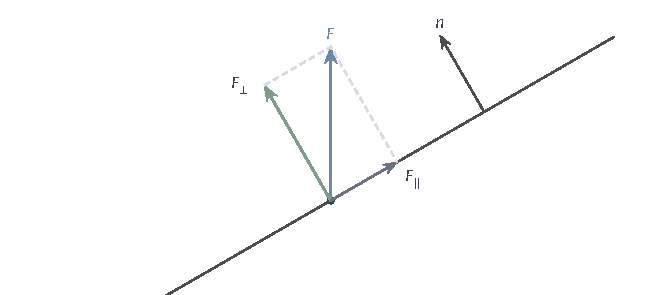
\includegraphics[width=112mm]{figures/00-shared/mathematical-preliminaries-upper/00-shared/tikz/chapter3-concept-processes/normal-projection.pdf}
 \caption{黑斜线表示局部切平面的一个截面，$n$为所选单位法向。向量$F$分为$F_\perp=(F^\top n)n$与切向部分$F_\parallel$；通量使用有符号标量$F^\top n$乘面积，切向部分不贡献。将$n$改为$-n$时标量分量变号，但投影向量$F_\perp$不变，这与直接把场反向不同。}
 \label{fig:analysis-process-normal-projection}
\end{figure}

连续向量场在紧曲面上有界，参数化的有向面积元也连续，因此每片通量都存在。切向分量不贡献通量；反转所选法向则使通量变号。

\subsubsection{积分的性质}

以下运算都在同一曲面、同一法向约定下进行，并假定各法向分量可积。
它们大多可归结为标量函数$\bm F^\top\bm n$的面积积分，直接沿用第一类积分的性质；与方向有关的法向反转和重参数化则需要单独说明。

\paragraph{加法}

向量场相加以后，其法向分量也相加，因此
\[
 \begin{aligned}
 \int_S(\bm F+\bm G)^\top\bm n\,\mathrm dS
 &=\int_S\bm F^\top\bm n\,\mathrm dS\\
 &\quad{}+\int_S\bm G^\top\bm n\,\mathrm dS.
 \end{aligned}
\]
绝对可积性由两项法向分量的绝对值之和控制，积分等式来自标量面积积分的加法性质。
物理上，两股水流叠加后穿过网的水量，等于两股水流分别穿过的水量之和。

\paragraph{减法}

向量场相减以后，其法向分量也相减，因此
\[
 \begin{aligned}
 \int_S(\bm F-\bm G)^\top\bm n\,\mathrm dS
 &=\int_S\bm F^\top\bm n\,\mathrm dS\\
 &\quad{}-\int_S\bm G^\top\bm n\,\mathrm dS.
 \end{aligned}
\]
两项法向分量绝对可积时，它们的差仍绝对可积，积分等式来自标量面积积分的减法性质。

\paragraph{数乘}

对实数$c$，由$(c\bm F)^\top\bm n=c(\bm F^\top\bm n)$，常数可以提出积分号：
\[
 \int_S(c\bm F)^\top\bm n\,\mathrm dS
 =c\int_S\bm F^\top\bm n\,\mathrm dS.
\]
这里缩放的是场，曲面的法向约定保持固定：流速加倍，穿过的水量也加倍。

\paragraph{曲面分割的可加性}

将$S$分为内部不重叠的有限片$S_1,\ldots,S_N$，并在每片采用原定向的限制，则
\[
 \int_S\bm F^\top\bm n\,\mathrm dS
 =\sum_{j=1}^N\int_{S_j}\bm F^\top\bm n\,\mathrm dS.
\]
零面积接缝不贡献积分。
关键在于每片沿用原来的法向：若某片单独反转法向，这一片计入的是反方向的穿越量，加起来就不再是整张曲面的通量。

\paragraph{法向反转}

在场和曲面不变时，把$\bm n$换成$-\bm n$会使通量变号：
\[
 \int_S\bm F^\top(-\bm n)\,\mathrm dS
 =-\int_S\bm F^\top\bm n\,\mathrm dS.
\]
水流本身没有变，变的只是计数方向：例如原法向朝上时，从下往上的穿越原来记为正，现在记为负。
这与第一类积分不同，后者不使用法向，换定向不改变结果。

\paragraph{重参数化}

更换参数时，所选的几何法向保持不变。
由定理~\ref{thm:analysis-surface-reparameterization}，新参数的叉积等于原叉积乘$\det\bm J_T$，
而二维换元公式使用的是$|\det\bm J_T|$。若$\det\bm J_T>0$，两者相同，式~\eqref{eq:analysis-surface-flux}右端不变；
若$\det\bm J_T<0$，例如交换两个参数，新叉积指向相反一侧，按定义中“方向相反时乘$-1$”的约定校正后，结果仍不变。
因此在固定曲面定向并完成这一校正后，通量只依赖曲面、定向和场，与参数选择无关。

\subsubsection{积分的计算}

计算通量分三步：先确定要用哪一侧的法向，再选一个叉积指向该侧的参数化（若指向相反，就在结果前加负号），最后在参数域上累计$\bm F$与有向面积元的内积。

对于图像曲面$z=\psi(x,y)$，第一类积分的计算中已经求出叉积
\[
 \bm r_x\times\bm r_y=(-\psi_x,-\psi_y,1)^\top,
\]
它的第三分量为正，指向上方。
因此取向上法向时，对$\bm F=(P,Q,R)^\top$有
\[
 \int_S\bm F^\top\bm n\,\mathrm dS
 =\iint_D(-P\psi_x-Q\psi_y+R)(x,y,\psi(x,y))\,\mathrm dx\,\mathrm dy.
\]
取向下法向则在右侧加负号。这一式直接使用有向面积元，叉积的长度已经与单位法向的分母抵消，不能再额外乘一次$\sqrt{1+\psi_x^2+\psi_y^2}$。

斜平面片是$\psi(x,y)=x+y$在单位正方形上的图像，可以用它核对通量与投影面积的关系。

\begin{example}[斜平面片上的竖直通量]
\label{ex:analysis-tilted-plane-flux}
取斜平面片$\bm r(u,v)=(u,v,u+v)^\top$、$E=[0,1]^2$和向上单位法向$(-1,-1,1)^\top/\sqrt3$。
对竖直单位场$\bm F=(0,0,1)^\top$，场与参数叉积$(-1,-1,1)^\top$的内积为$1$，故
\[
 \int_S\bm F^\top\bm n\,\mathrm dS
 =\int_0^1\int_0^1 1\,\mathrm du\,\mathrm dv=1.
\]
用面积分开看：这块面的面积为$\sqrt3$（示例~\ref{ex:analysis-tilted-plane-area}），场的法向分量为$\bm F^\top\bm n=1/\sqrt3$，两者相乘为$1$，恰好等于它在$xy$平面上的投影面积。
\end{example}

同样地，平面$z=ax+by+c$在单位圆盘$D$上方的部分对该场的向上通量为$\iint_D1\,\mathrm dx\,\mathrm dy=\pi$，
等于水平投影面积；它的实际面积则为$\pi\sqrt{1+a^2+b^2}$。
这与示例~\ref{ex:analysis-tilted-square-flux}中倾斜屋顶接雨的结果一致：竖直的流只“看见”曲面的水平投影。

对半径为$R$的球面，讨论单位法向量时已算出$(\varphi,\theta)$次序的参数叉积为$R\sin\varphi\,\bm r$，它在参数域内部指向外侧。
下面三个例子都取外法向，依次计算径向场、点源场和恒定场的通量。

\begin{example}[径向场穿过球面]
\label{ex:analysis-radial-field-sphere-flux}
令$\bm F(\bm x)=\bm x/R$。在球面上$\bm F$恰等于外单位法向，$\bm F^\top\bm n=1$，由示例~\ref{ex:analysis-sphere-area}，
\[
 \int_S\bm F^\top\bm n\,\mathrm dS
 =\int_S1\,\mathrm dS=4\pi R^2.
\]
取内法向时通量为$-4\pi R^2$。
\end{example}

这次外向通量与面积相等，是因为法向分量处处为$1$。
一般情形下$|\bm F^\top\bm n|\leq\lVert\bm F\rVert_2$，通量的绝对值不超过场的大小对面积的积分；场的方向偏离法向时，只有法向分量计入通量。

接下来的两个例子形成对比：一个场由原点处的点源发出，另一个场在空间中处处相同。

\begin{example}[点源场的通量与半径无关]
\label{ex:analysis-point-source-sphere-flux}
令$\bm F(\bm x)=\bm x/\lVert\bm x\rVert_2^3$（$\bm x\neq\bm0$），$S$是以原点为中心、半径为$R$的球面，外法向为$\bm n=\bm x/R$。
$\bm F$在不含原点的球面上连续，因而法向分量可积。
在$S$上$\lVert\bm x\rVert_2=R$，故
\[
 \bm F^\top\bm n=\frac{\bm x^\top\bm x}{R^3\cdot R}=\frac1{R^2},
\]
外向通量为$(1/R^2)\cdot4\pi R^2=4\pi$。
\end{example}

球面越大，场越弱，但面积增大的倍数恰好抵消场的减弱，所以通量不随$R$改变：
以点源为中心的球面无论多大，测得的点源单位时间放出的总量都一样。

\begin{example}[恒定场穿过球面的净通量为零]
\label{ex:analysis-constant-field-sphere-flux}
令$\bm F=(0,0,1)^\top$。由$\bm r_\varphi\times\bm r_\theta=R\sin\varphi\,\bm r$，被积函数为
$\bm F^\top(\bm r_\varphi\times\bm r_\theta)=R\sin\varphi\cdot R\cos\varphi=R^2\sin\varphi\cos\varphi$，于是
\[
 \int_S\bm F^\top\bm n\,\mathrm dS
 =\int_0^{2\pi}\int_0^\pi R^2\sin\varphi\cos\varphi\,\mathrm d\varphi\,\mathrm d\theta=0.
\]
分开计算，上半球面$0\leq\varphi\leq\pi/2$的外向通量为
\[
 2\pi R^2\int_0^{\pi/2}\sin\varphi\cos\varphi\,\mathrm d\varphi=\pi R^2,
\]
下半球面$\pi/2\leq\varphi\leq\pi$的外向通量为$-\pi R^2$。
\end{example}

在恒定场中，水从下半球面流入球内，又从上半球面等量流出，球内既不产生也不吸收水，所以闭曲面的净通量为零。
包围点源的球面则有正的净通量。
可见闭曲面的净通量反映它所围区域内部的源与汇；
第~\ref{sec:multivariable-boundary-relations}节将用区域内部的散度累计来计算闭曲面的通量，并核对这里的几个结果。

\FloatBarrier

\section{向量场与微分算子}

定义~\ref{def:multivariable-gradient}把标量函数的各个一阶偏导数排成梯度。现在考虑开集$U$上的向量场$\bm F$，不妨把它想成流体的速度场：$\bm F(\bm x)$是流体在位置$\bm x$处的速度。
对这样的场，有两个自然的局部问题：在一点附近，流体是净流出还是净流入；流体是否绕这一点打转。
两个问题的答案都由$\bm F$各分量的一阶偏导数决定，但用到的偏导数组合不同。
回答前一个问题的是散度，回答后一个问题的是旋度，二者都以向量场为输入；随后的Laplace算子以标量函数为输入，比较函数在一点的值与周围平均值的差别。

\subsection{散度与局部通量}

\paragraph{小立方体的净流出}

设$\bm F=(F_1,F_2,F_3)^\top$是三维流体的速度场。第~\ref{sec:analysis-surface-integration}节定义的通量只取速度的法向分量，原因如下。

在很短的时间$\Delta t$内，穿过面积为$\Delta S$、单位法向为$\bm n$的一小片曲面的流体，占据一个底面积为$\Delta S$、高约为$(\bm F^\top\bm n)\Delta t$的斜柱；所以单位时间穿过这一小片的流体体积约为$(\bm F^\top\bm n)\Delta S$，速度的切向分量只让流体沿曲面滑动，不贡献穿过量。
现在以点$\bm a$为中心取边长为$h$的小立方体，各面与坐标平面平行，估计单位时间从它流出的净体积。

先看与$x$轴垂直的两张面。右面$x=a_1+h/2$的外法向是$\bm e_1$，场在这张面上的法向分量是$F_1$；用面中心的值代表整张面，流出量约为$F_1(\bm a+\tfrac h2\bm e_1)h^2$。
左面$x=a_1-h/2$的外法向是$-\bm e_1$，流出量约为$-F_1(\bm a-\tfrac h2\bm e_1)h^2$；$F_1>0$时这个量为负，表示沿$x$正方向的流动在左面是流入。两面合计为
\[
 \Bigl[F_1\bigl(\bm a+\tfrac h2\bm e_1\bigr)-F_1\bigl(\bm a-\tfrac h2\bm e_1\bigr)\Bigr]h^2
 \approx \partial_1F_1(\bm a)\,h\cdot h^2,
\]
这里用偏导数乘距离$h$近似了$F_1$在两张面中心之间的差。
若$F_1$沿$x$方向增大，从右面的有向流出量与左面的有向流出量之和为正，这对面贡献正的净流出；若$F_1$沿$x$方向不变，流入与流出恰好相等。

另外两对面同样分别给出约$\partial_2F_2(\bm a)h^3$和$\partial_3F_3(\bm a)h^3$。六张面合计后除以体积$h^3$，得到
\[
 \frac{\text{小立方体的净流出}}{\text{小立方体的体积}}
 \approx\partial_1F_1(\bm a)+\partial_2F_2(\bm a)+\partial_3F_3(\bm a).
\]
当$\bm F$连续可微时，可把它在整个小立方体上统一展开为$\bm F(\bm a)+D\bm F(\bm a)(\bm x-\bm a)+o(h)$。每张面的面积为$h^2$，余项对六张面通量的总贡献是$o(h^3)$；常数项在相对两面抵消，线性项给出上面的三个偏导数。除以$h^3$再令$h\to0$，便得到所述极限，无需先使用整个区域上的Gauss公式。右侧的偏导数之和称为散度。
\begin{definition}[散度]
\label{def:multivariable-divergence}
设$U\subseteq\mathbb R^d$为开集，$\bm F=(F_1,\ldots,F_d)^\top:U\to\mathbb R^d$的各分量一阶偏导数存在。
$\bm F$的\term{散度}（divergence）是标量函数
\[
 \operatorname{div}\bm F
 =\nabla\mathbin{\cdot}\bm F
 =\sum_{j=1}^d\partial_jF_j.
\]
\end{definition}
当$\bm F$可微时，这个和也等于Jacobian矩阵$D\bm F$的迹。它只累计对应坐标方向的变化率；非对角偏导数不直接进入净流出率。

\paragraph{源的强度}

按小立方体上的推导，散度是单位体积的净流出率，可以理解为一点处“源”的强度。
$\operatorname{div}\bm F(\bm a)>0$表示$\bm a$附近像有一个源，流体在这里产生并向外流走；$\operatorname{div}\bm F(\bm a)<0$表示这里像一个汇，流入的多于流出的；散度为零表示流入与流出平衡。
若流体不可压缩，内部又没有注入或抽出流体的源和汇，则每个小体积的流入量都等于流出量，速度场的散度处处为零。

下面三个场分别对应均匀膨胀、绕轴转动和整体平移，可以用来检验这一解释。
\begin{example}[径向场、旋转场与常场的散度]
三维径向场$\bm F(x,y,z)=(x,y,z)^\top$满足$\partial_xF_1=\partial_yF_2=\partial_zF_3=1$，所以$\operatorname{div}\bm F=1+1+1=3$：流体从各处均匀地向外膨胀，每单位体积每单位时间多出$3$个单位体积的流体。

旋转场$\bm G(x,y,z)=(-y,x,0)^\top$的第一分量不含$x$，第二分量不含$y$，第三分量为零，所以$\operatorname{div}\bm G=0+0+0=0$：流体绕$z$轴转动，任何小立方体流入多少就流出多少。

常场$\bm H=(1,0,0)^\top$的各分量都是常数，散度同样为$0$：流体整体平移，每个小立方体从左面流入的量都从右面流出。
\end{example}
旋转场和常场都不是零场，散度却都为零。可见散度为零只表示局部净流出率为零，并不表示向量场为零。

二维场$(P,Q)^\top$的散度相应为$P_x+Q_y$，它是小正方形四条边上的净流出除以面积所得的极限；定理~\ref{thm:multivariable-planar-flux}的平面通量公式使用这一标量函数。

\subsection{旋度与局部环流}

\paragraph{小正方形上的环流}

净流出不能描述绕一点旋转的运动。旋转场$\bm G=(-y,x,0)^\top$的散度为零，但在水平平面内沿以$z$轴上一点为圆心的圆周逆时针走一圈，场始终与行进方向相同，环流不为零。
为了度量一点附近的旋转，先在平面上计算小正方形边界的环流。

设平面场为$(P,Q)^\top$，以$\bm a$为中心取边长为$h$的正方形，沿逆时针方向走一圈。

下边从左向右，切向分量是$P$，贡献约$P(\bm a-\tfrac h2\bm e_2)h$；上边从右向左，贡献约$-P(\bm a+\tfrac h2\bm e_2)h$；两者合计约$-\partial_yP(\bm a)h^2$。
右边从下向上，贡献约$Q(\bm a+\tfrac h2\bm e_1)h$；左边从上向下，贡献约$-Q(\bm a-\tfrac h2\bm e_1)h$；两者合计约$\partial_xQ(\bm a)h^2$。四边相加后除以面积$h^2$，得到
\[
 \frac{\text{小正方形边界的逆时针环流}}{\text{小正方形的面积}}
 \approx\partial_xQ(\bm a)-\partial_yP(\bm a).
\]
两项的符号可以这样理解。若$Q$沿$x$方向增大，右边向上的流速比左边大，这一对边推动逆时针转动；若$P$沿$y$方向增大，上边向右的流速比下边大，这一对边推动顺时针转动，所以$\partial_yP$带负号。

在三维空间中，小正方形可以放在分别垂直于三个坐标轴的平面里，行进方向都取从相应坐标轴正方向看的逆时针。
垂直于$z$轴时，平面坐标是$(x,y)$，$(F_1,F_2)$相当于$(P,Q)$，同样的计算给出$\partial_xF_2-\partial_yF_1$；
垂直于$x$轴时，平面坐标的次序是$(y,z)$，$(F_2,F_3)$相当于$(P,Q)$，得到$\partial_yF_3-\partial_zF_2$；
垂直于$y$轴时，平面坐标的次序是$(z,x)$，$(F_3,F_1)$相当于$(P,Q)$，得到$\partial_zF_1-\partial_xF_3$。
这样选取坐标次序，是因为$\bm e_2\times\bm e_3=\bm e_1$、$\bm e_3\times\bm e_1=\bm e_2$：从坐标轴正方向看，第一个平面坐标轴逆时针转过直角得到第二个。
把这三个环流率按$x,y,z$轴的次序排成一个向量，就得到旋度。
\begin{definition}[旋度]
\label{def:multivariable-curl}
设$U\subseteq\mathbb R^3$为开集，$\bm F=(F_1,F_2,F_3)^\top:U\to\mathbb R^3$的各分量一阶偏导数存在。
$\bm F$的\term{旋度}（curl）是向量场
\[
 \operatorname{curl}\bm F=\nabla\times\bm F
 =\begin{pmatrix}
   \partial_yF_3-\partial_zF_2\\
   \partial_zF_1-\partial_xF_3\\
   \partial_xF_2-\partial_yF_1
  \end{pmatrix}.
\]
\end{definition}

\paragraph{旋转的轴与强度}

坐标平面上的三个计算可以推广到任意方向。

设$\bm F$连续可微，$\bm n$是单位向量；在过点$\bm a$且垂直于$\bm n$的平面内，取以$\bm a$为中心的小正方形或小圆周，从$\bm n$的箭头一侧看按逆时针行进。
尺寸趋于零时，环流除以所围面积的极限等于$(\operatorname{curl}\bm F)(\bm a)^\top\bm n$。$\bm n$为坐标轴方向时，这就是上面的计算；一般方向的证明放在Stokes公式之后。

由Cauchy--Schwarz不等式，$(\operatorname{curl}\bm F)^\top\bm n\leq\lVert\operatorname{curl}\bm F\rVert_2$；旋度不为零时，等号当且仅当$\bm n$与旋度同向时成立。
所以旋度的方向是局部旋转最强的转轴，其长度是旋转的强度；转向由右手定则确定：右手大拇指沿旋度方向，其余四指弯曲的方向就是转向。

一个物理图像是放进流水中的小桨轮。让桨轮的转轴沿$\bm n$，水流沿轮缘推动各个叶片；桨轮是否转动、往哪边转，取决于沿轮缘的环流，也就是$(\operatorname{curl}\bm F)^\top\bm n$的符号；转轴与旋度平行时转得最快。
这一图像帮助理解定义，但不代替上面的计算。

先用整体转动和径向膨胀检验这一图像。
\begin{example}[刚体旋转与径向膨胀的旋度]
\label{ex:analysis-rigid-rotation-curl}
整体以角速度$\omega$绕$z$轴旋转的流体，速度场为$\bm F=\omega(-y,x,0)^\top$。代入定义，前两个分量$\partial_yF_3-\partial_zF_2$与$\partial_zF_1-\partial_xF_3$都为零，第三个分量为$\partial_x(\omega x)-\partial_y(-\omega y)=2\omega$，所以$\nabla\times\bm F=(0,0,2\omega)^\top$。
特别地，$\omega=1/2$时$\bm F=(-y/2,x/2,0)^\top$，旋度为$(0,0,1)^\top$。

径向场$(x,y,z)^\top$的第$i$个分量只依赖第$i$个坐标，旋度定义中的每个交叉偏导数都为零，所以旋度为零：流体只向外膨胀而不打转。
\end{example}
刚体旋转的旋度沿转轴，长度是角速度的两倍，与桨轮图像一致。不过，旋度与流线是否弯曲并不是一回事，下面两个场从相反的方向说明这一点。
\begin{example}[剪切流与涡旋场]
剪切流$\bm F=(y,0,0)^\top$的流线都是水平直线。它的偏导数中只有$\partial_yF_1=1$不为零，所以$\nabla\times\bm F=(0,0,-1)^\top$。
物理上，上方的水比下方的水向右流得快，桨轮的上缘被推得更多，从$z$轴正方向看桨轮顺时针转动，与第三分量为负一致。

再看平面上沿同心圆流动的场。

设流体在每个以原点为圆心的圆周上逆时针流动，半径为$r$的圆周上速率为$s(r)>0$，其中$s$可微，即
\[
 \begin{gathered}
(P,Q)^\top=g(r)\,(-y,x)^\top\\
g(r)=\frac{s(r)}r\\
r=\sqrt{x^2+y^2}>0.
 \end{gathered}
\]
由$\partial_xr=x/r$、$\partial_yr=y/r$，有$Q_x=g(r)+g'(r)x^2/r$、$P_y=-g(r)-g'(r)y^2/r$，所以
\[
 Q_x-P_y=2g(r)+rg'(r)=\frac{s(r)}r+s'(r).
\]
第一项$s(r)/r$来自流线的弯曲，第二项$s'(r)$来自不同半径上流速的差别。刚体旋转$s(r)=\omega r$时两项都等于$\omega$，合计$2\omega$，与前例一致。
第~\ref{sec:multivariable-potential-path-independence}节穿孔平面上的涡旋场$(-y,x)^\top/(x^2+y^2)$对应$s(r)=1/r$，两项分别为$1/r^2$与$-1/r^2$，所以在原点以外$Q_x-P_y=0$。
\end{example}
剪切流的流线是直线，旋度却不为零；涡旋场的流线弯曲，在原点以外旋度却为零。后者的原因是：流线弯曲带来的逆时针倾向，恰好被外侧流速较慢带来的顺时针倾向抵消，所以放在原点以外的小桨轮不转。

对二维场$(P,Q)^\top$，平面内需要的是标量$Q_x-P_y$。
把二维场补上为零的第三分量，写成三维场$(P,Q,0)^\top$后，这一标量正是旋度的第三分量，也就是旋度在向上法向$\bm e_3$上的分量。
符号$\nabla\mathbin\cdot$和$\nabla\times$表示这里定义的偏导数组合，不是两个普通数值向量的内积或叉积。


图~\ref{fig:analysis-process-divergence-circulation-fields}在同一个单位圆周上分别观察净流出与切向环流，比较两种微分算子所记录的信息。
\begin{figure*}[!htbp]
 \centering
 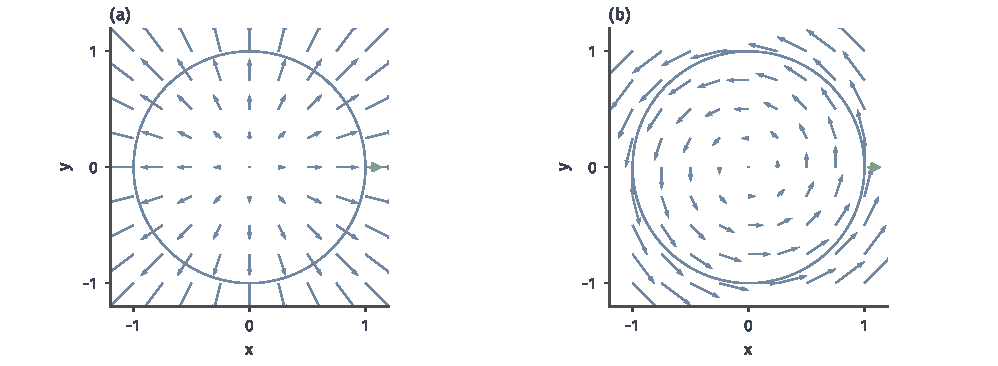
\includegraphics[width=169.0mm]{figures/00-shared/mathematical-preliminaries-upper/00-shared/matplotlib/chapter3-concept-processes/divergence-circulation-fields.pdf}
 \caption{(a) 径向场$(x,y)^\top$的二维散度为$2$、旋转率$Q_x-P_y=0$，圆周外向通量为$2\pi$、环流为零。(b) 旋转场$(-y,x)^\top$的散度为零、旋转率为$2$，通量为零、环流为$2\pi$。绿箭头仅标记外法向；蓝色场箭头按相同常数缩放。零散度不等于零场，也不等于零环流。}
 \label{fig:analysis-process-divergence-circulation-fields}
\end{figure*}

\subsection{Laplace算子与运算关系}

标量函数的梯度是向量场，因此可以对它继续取散度，把各坐标方向的二阶变化相加。
这一复合运算出现在多元分部积分中，也出现在描述热传导和扩散的方程中；它的输入与输出都是标量函数。
\begin{definition}[Laplace算子]
\label{def:multivariable-laplacian}
对开集$U\subseteq\mathbb R^d$上的二阶连续可微标量函数$v$，定义\term{Laplace算子}（Laplacian）为
\[
 \Delta v=\operatorname{div}(\nabla v)
 =\sum_{j=1}^d\partial_j^2v.
\]
\end{definition}
梯度把标量函数变为向量场，散度再把向量场变为标量函数，所以$\Delta v$仍是标量函数；它与输入、输出都是向量场的旋度属于不同类型的运算。

从矩阵表示看，$\Delta v$也是Hessian矩阵的迹。例如$v(\bm x)=\|\bm x\|_2^2$的Hessian为$2\bm I$，所以$\Delta v=2d$。

三个算子还有两条由混合偏导交换直接得到的关系。在三维开集上，若$v\in C^2$，则
\[
 \operatorname{curl}(\nabla v)=\bm0.
\]
例如第三分量是$\partial_x\partial_yv-\partial_y\partial_xv=0$，另两个分量同理。反向由无旋推势函数仍须核对定义域；星形域与有孔域的区别已在路径无关一节说明。

若向量场$\bm F\in C^2$，则
\[
 \operatorname{div}(\operatorname{curl}\bm F)=0.
\]
将旋度的三个分量代入散度，得到六个二阶混合偏导，每一项都与交换求导次序后的另一项异号相消。这里第一个等式的输入是标量函数、输出是零向量，第二个的输入是向量场、输出是零标量，不能混淆对象类型。

\paragraph{与邻域平均值的差}

一元情形中，$v''(a)>0$表示函数在$a$附近向上弯，$v(a)$低于两侧邻点的平均值。多元情形可以做同样的比较。
在$\bm a$的每个坐标方向上各取前后两个邻点$\bm a\pm h\bm e_j$，沿该坐标作二阶Taylor展开：
\[
 v(\bm a+h\bm e_j)+v(\bm a-h\bm e_j)-2v(\bm a)=h^2\partial_j^2v(\bm a)+o(h^2),
\]
一阶项$\pm h\partial_jv(\bm a)$在两点相加时抵消。对$j=1,\ldots,d$求和，再除以邻点个数$2d$，得到
\[
 \frac1{2d}\sum_{j=1}^d\bigl[v(\bm a+h\bm e_j)+v(\bm a-h\bm e_j)\bigr]-v(\bm a)
 =\frac{h^2}{2d}\Delta v(\bm a)+o(h^2).
\]
因此，$h$足够小时，$\Delta v(\bm a)>0$表示$v(\bm a)$低于周围邻点的平均值，$\Delta v(\bm a)<0$表示高于平均值；$\Delta v(\bm a)=0$表示二者之差是$o(h^2)$，在这一精度下相等。

下面用两个二次函数直接比较邻点平均值与中心值。
\begin{example}[二次函数的邻点平均]
取$v(x,y,z)=x^2+y^2+z^2$，则$\Delta v=2+2+2=6$。在原点，$v(\bm0)=0$；六个邻点$\pm h\bm e_j$上的值都是$h^2$，所以邻点平均值比中心值高$h^2$，恰等于$\frac{h^2}{2d}\Delta v=\frac{h^2}6\cdot6$。二次函数的Taylor展开没有余项，等式精确成立。

再取$v(x,y)=x^2-y^2$，则$\Delta v=2-2=0$。原点的四个邻点$(\pm h,0)$与$(0,\pm h)$上的取值为$h^2,h^2,-h^2,-h^2$，平均值恰为$0=v(\bm0)$。
\end{example}
第二个函数在$x$方向向上弯、在$y$方向向下弯，两种弯曲正好抵消。Laplace算子记录的是各坐标方向弯曲的总和，不能据此判断每个方向各自的弯曲。

\paragraph{热传导中的含义}

设$u(t,\bm x)$是时刻$t$物体内位置$\bm x$处的温度，它对$\bm x$二阶连续可微。热量从高温处流向低温处，Fourier热传导定律把单位时间穿过单位面积的热流写成$\bm q=-k\nabla u$，其中常数$k>0$为导热系数，$\nabla$只作用于空间变量$\bm x$\scite{math-openstax-calculus3}。
由散度的含义，单位体积的热量净流出率为$\operatorname{div}\bm q=-k\Delta u$。没有热源时，单位体积内热量的增加率等于净流入率$-\operatorname{div}\bm q=k\Delta u$；再除以单位体积的热容$c>0$，得到温度的变化率
\[
 \partial_tu=\frac kc\,\Delta u,
\]
这就是热传导方程。

这个方程说明温度怎样随时间变化。比周围平均更冷的点满足$\Delta u>0$，会从周围吸收热量而升温；比周围平均更热的点满足$\Delta u<0$，会降温；温度分布因而逐渐被抹平。
温度不再随时间变化时，处处有$\Delta u=0$；按邻域平均值的公式，每点的温度在上述精度下等于周围的平均。这里的Fourier定律是物理模型，本节只用它说明$\Delta$的含义。

\section{区域与边界的积分关系}
\label{sec:multivariable-boundary-relations}

一元微积分基本定理说，若$f$在$[a,b]$上连续可微，则导数$f'$在区间上的积分等于$f(b)-f(a)$：区间内部各点的变化率累计起来，只剩下两个端点上的函数值。
区间的边界就是这两个端点，所以$f(b)-f(a)$也可以读成带符号的边界求和：右端点记正号，左端点记负号。
路径积分基本定理（式~\eqref{eq:analysis-line-integral-gradient}）把同样的关系搬到路径上：梯度场沿路径的积分，等于势函数在终点与起点的值之差。

本节把这种“内部导数的累计等于边界上的累计”的关系推广到平面区域、空间区域和曲面。
三种推广共用一个思路。先把对象切成许多小块；在每个小块上，某个导数乘小块的大小，近似等于向量场沿小块边界的累计。
相邻两块的公共边界被两块各算一次，两次的方向相反，相加后抵消，最后只剩下整个对象的外边界。
按边界的类型，本节回答三个问题：平面区域上的积分何时等于边界路径积分，这是Green公式；空间区域上的积分何时等于边界曲面积分，这是Gauss公式；曲面上的积分何时等于曲面边界的路径积分，这是Stokes公式。

这些公式中的被积对象不能互换。沿边界的环流累计向量场的切向分量，对应的内部量是旋度，它衡量场绕一点旋转的强度；
穿过边界的通量累计向量场的法向分量，对应的内部量是散度，它衡量场从一点向外发散的强度。

前一节已从局部变化定义散度、旋度与Laplace算子。下面先规定边界的方向，再给出内部与边界之间的积分关系。
所有参数积分沿用本章的Riemann积分。经典公式的组织参考向量微积分教材\scite{math-openstax-calculus3}。

\paragraph{边界的定向}

将一个区域分成相邻小块时，公共边或公共面不属于原区域的外边界。
要使这些内部贡献相消，各小块必须采用相容的方向；同时，每个小块的方向还要与小块上局部计算所用的方向一致：环流按逆时针计算，通量按外法向计算。
下面依次规定平面区域边界的行进方向、区域边界的外法向，以及定向曲面边界的行进方向。

\paragraph{平面区域的正向边界}

平面区域的边界是路径，所以先规定沿边界行进的方向。本节考虑的平面区域，边界由若干条简单闭曲线组成；简单闭曲线指除首尾相合外不自交的闭曲线。
对有界平面区域，取边界方向使沿曲线前进时区域总在左侧，称为正向边界。
沿单位圆逆时针行走，单位圆盘始终在左手边，所以圆盘的正向边界是逆时针方向。

有孔洞时，外边界仍是逆时针；围绕孔洞的内边界要使区域而非孔洞留在左侧，因而是顺时针。
例如圆环$1<x^2+y^2<4$的外圈$r=2$逆时针、内圈$r=1$顺时针，两圈边界方向相反。
这个约定与小块相消的要求一致：把圆环切成许多小块，每块都按逆时针走边界，内部公共边相互抵消后，剩在孔洞边上的那些边恰好被顺时针走过。

边界由多段光滑弧组成时，按这一方向逐段相接，转角处不另加积分项。
一般地，相邻平面小块各自采用正向边界时，共同边被沿相反方向走过，两个有向路径积分恰好抵消。

\paragraph{区域边界的外法向}

通量需要的是法向，而不是边界的行进方向。空间区域的外单位法向从内部指向外部；有孔洞时，孔洞边界的外法向指向孔洞。
例如球壳$1<\lVert\bm x\rVert_2<2$在外球面上的外法向背离原点，在内球面上的外法向指向原点。
相邻子区域的公共面上，两侧子区域的外法向相反，所以内部通量相消。

平面区域边界上的外单位法向按同样方式规定，只是通量沿边界按弧长累计。
外法向与正向边界的单位切向量$\bm\tau=(\tau_1,\tau_2)^\top$有固定关系：区域在行进方向的左侧，外侧就在右侧，所以把$\bm\tau$顺时针转过直角就得到外法向$\bm n=(\tau_2,-\tau_1)^\top$。
例如在单位圆的点$(1,0)$处，逆时针的切向量是$(0,1)^\top$，按此公式得到$(1,0)^\top$，确实指向圆外。

\paragraph{定向曲面边界的诱导方向}

曲面取定单位法向$\bm n$后，其边界路径的方向不能再任意选择。
边界的正向按右手约定确定：右手大拇指朝法向，其余手指弯曲的方向为正向，称为由法向诱导的方向，简称诱导方向。
等价地，沿边界前进并把头朝向法向时，曲面留在左侧。面朝前进方向$\bm f$、头顶朝$\bm u$站立时，左手方向是$\bm u\times\bm f$；用这个叉积可以核对具体例子。

下面用这个叉积核对两张以单位圆为边界的曲面，后面检验Stokes公式时会用到它们。
\begin{example}[向上圆盘与外向上半球面的诱导方向]
\label{ex:analysis-hemisphere-induced-orientation}
对取向上法向$\bm e_3$的单位圆盘，在边界点$(1,0,0)$处取前进方向$\bm f=\bm e_2$，左手方向为$\bm e_3\times\bm e_2=-\bm e_1$，指向圆盘内部。所以诱导方向是从上方看逆时针。

对取外法向的上半单位球面，赤道上的点$(1,0,0)$处外法向是$\bm e_1$。同样取前进方向$\bm f=\bm e_2$，左手方向为$\bm e_1\times\bm e_2=\bm e_3$，正指向半球面所在的上方。所以它的诱导方向也是从上方看逆时针，与向上圆盘的边界方向相同。
\end{example}
两张曲面在边界点处的法向不同，曲面伸出的方向也不同；但二者都满足“头朝法向时曲面在左侧”，所以诱导出同一个边界方向。

若翻转曲面法向，边界的诱导方向也随之翻转。分片曲面的定向相容，指相邻曲面片在公共边上诱导出相反的行进方向。
这时公共边上的路径积分相消，只留下整张曲面的真正边界。


图~\ref{fig:analysis-process-boundary-orientation-cancellation}把相容方向的作用画出来：只有内部公共边相消，才会只剩下整个对象的外边界。
\begin{figure}[!htbp]
 \centering
 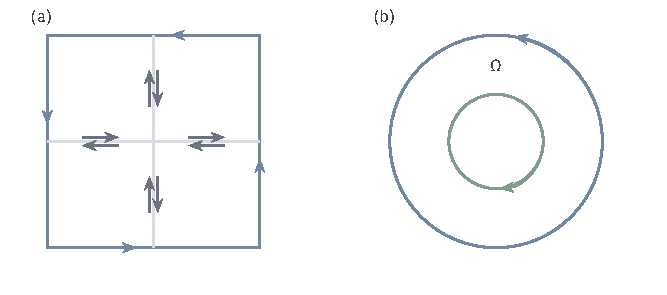
\includegraphics[width=112mm]{figures/00-shared/mathematical-preliminaries-upper/00-shared/tikz/chapter3-concept-processes/boundary-orientation-cancellation.pdf}
 \caption{(a) 四个小正方形各取逆时针正向，共同边被沿相反方向走过；灰箭头略错开以便辨认，实际是同一条边。相加后只留下蓝色外边界。(b) 圆环的外边界逆时针、孔洞边界顺时针，沿任一边界前进时区域均在左侧。曲面拼片时也按公共边相反方向保证Stokes边界项相消。}
 \label{fig:analysis-process-boundary-orientation-cancellation}
\end{figure}

\subsection{Green公式与平面边界}

在平面上，区域的边界是一维路径。对同一个二维向量场，可以沿边界累计切向分量，得到环流；也可以累计外法向分量，得到通量。
两种边界积分分别对应区域内部的$Q_x-P_y$和散度$P_x+Q_y$。

\subsubsection{Green公式的环流形式}

旋度一节在小正方形上算出：逆时针环流约等于$Q_x-P_y$乘正方形面积。
把区域$\Omega$划分成许多小正方形（靠近弯曲边界处是不规则的小块），对每块写出这一近似再相加。
相邻两块的公共边在两块中方向相反，贡献抵消，剩下的只有沿$\Omega$正向边界的环流；另一侧各块“$Q_x-P_y$乘面积”之和，则是区域积分的近似和。
Green公式说明，在适当条件下这一近似在加细后成为精确等式：区域内各处微小旋转的累计，等于沿边界走一圈的总环流。
\begin{theorem}[Green公式]
\label{thm:multivariable-green}
设$\Omega\subseteq\mathbb R^2$为有界开区域，边界由有限条分段$C^1$简单闭曲线组成，
且区域在每段光滑边界附近位于边界的一侧。边界取正向，即外边界逆时针、孔洞边界顺时针。
若二维向量场$\bm F=(P,Q)^\top$在$\overline\Omega$的开邻域内连续可微，则\term{Green公式}（Green's theorem）给出
\begin{equation}
 \oint_{\partial\Omega}P\,\mathrm dx+Q\,\mathrm dy
 =\iint_\Omega\left(\frac{\partial Q}{\partial x}-\frac{\partial P}{\partial y}\right)\,\mathrm dx\,\mathrm dy.
 \label{eq:multivariable-green}
\end{equation}
\end{theorem}
左侧是向量场的切向路径积分；右侧是标量函数$Q_x-P_y$的区域积分。
在矩形上，二者的等式可以直接由一元基本定理和连续函数的累次积分公式推出。
\begin{proof}[矩形情形的证明]
取$\Omega=(a,b)\times(c,d)$，先写出左侧沿四条边的贡献。下边$(t,c)$、$a\leq t\leq b$从左向右，$\mathrm dy=0$，贡献$\int_a^bP(x,c)\,\mathrm dx$；
上边从$(b,d)$走到$(a,d)$，贡献$-\int_a^bP(x,d)\,\mathrm dx$；右边从下向上，贡献$\int_c^dQ(b,y)\,\mathrm dy$；左边从上向下，贡献$-\int_c^dQ(a,y)\,\mathrm dy$。
水平边上$\mathrm dy=0$，竖直边上$\mathrm dx=0$，所以$Q$只在竖直边出现，$P$只在水平边出现。

再看右侧。场在闭矩形附近连续可微，以下被积函数均可积。固定$x$，对$y$用一元基本定理得$\int_c^d\partial_yP(x,y)\,\mathrm dy=P(x,d)-P(x,c)$；再对$x$积分，并由连续函数的累次积分公式换成区域积分。对$Q$则先固定$y$、对$x$积分。于是
\[
 \begin{aligned}
 -\iint_\Omega\partial_yP\,\mathrm dx\,\mathrm dy
 &=\int_a^b[P(x,c)-P(x,d)]\,\mathrm dx,\\
 \iint_\Omega\partial_xQ\,\mathrm dx\,\mathrm dy
 &=\int_c^d[Q(b,y)-Q(a,y)]\,\mathrm dy.
 \end{aligned}
\]
第一行恰是下边与上边的两项，第二行恰是右边与左边的两项。
四项合起来，正是沿下、右、上、左四条边逆时针行进得到的路径积分。
\end{proof}
有限个矩形拼接时，公共边上的积分因方向相反而抵消。
一般规则区域的证明还需处理区域分片及边界逼近误差，不能仅凭小矩形上的等式完成；这里引用一般形式，完整论证可参考向量微积分教材\scite{math-strang1991calculus}。

先用旋转场在单位圆盘上核对公式两侧，并观察边界方向的作用。
\begin{example}[旋转场在单位圆盘上的Green公式]
\label{ex:analysis-rotation-field-green-disk}
取$\bm F=(P,Q)^\top=(-y,x)^\top$，$\Omega$为单位圆盘。$\bm F$在整个平面上连续可微，定理条件满足。
右侧被积函数为$Q_x-P_y=1-(-1)=2$，区域积分为$2\cdot\pi=2\pi$。
左侧取逆时针边界$\gamma(t)=(\cos t,\sin t)^\top$，$0\leq t\leq2\pi$，则$\bm F(\gamma(t))^\top\gamma'(t)=\sin^2t+\cos^2t=1$，积分同样为$2\pi$。
若把圆周改为顺时针，左侧变为$-2\pi$，右侧仍为$2\pi$，等式不再成立。
\end{example}
区域积分不含方向信息，边界积分却随方向反转而变号；Green公式的符号由正向边界的约定决定。

Green公式也可以反过来使用：选一个满足$Q_x-P_y\equiv1$的场，右侧就是区域的面积，于是面积可以由边界环流算出。
\begin{example}[用边界计算面积]
\label{ex:analysis-green-area-formula}
设$\Omega$满足定理~\ref{thm:multivariable-green}的条件。取$P=-y/2$、$Q=x/2$，则$Q_x-P_y=1$，Green公式给出
\[
 \operatorname{area}(\Omega)=\frac12\oint_{\partial\Omega}x\,\mathrm dy-y\,\mathrm dx.
\]
对半轴为$\alpha,\beta>0$的椭圆区域，正向边界取$\gamma(t)=(\alpha\cos t,\beta\sin t)^\top$、$0\leq t\leq2\pi$。这时$\mathrm dx=-\alpha\sin t\,\mathrm dt$、$\mathrm dy=\beta\cos t\,\mathrm dt$，
\[
 x\,\mathrm dy-y\,\mathrm dx=(\alpha\beta\cos^2t+\alpha\beta\sin^2t)\,\mathrm dt=\alpha\beta\,\mathrm dt,
\]
所以面积为$\frac12\cdot2\pi\alpha\beta=\pi\alpha\beta$。
\end{example}
这个公式只需要沿边界走一圈、记录坐标与位移，就能得到所围面积；机械求积仪正是按这一原理工作的。

定理要求场在$\overline\Omega$的开邻域内连续可微。区域包含场的奇点时，这一条件不再满足，下面的例子说明它不能省略。
\begin{example}[有孔区域上的涡旋场]
\label{ex:analysis-annulus-vortex-green}
第~\ref{sec:multivariable-potential-path-independence}节的穿孔平面反例中，$\bm F=(-y,x)^\top/(x^2+y^2)$在原点以外满足$Q_x-P_y=0$，但沿单位圆逆时针一周的环流为$2\pi$。

取圆环$\Omega=\{1<x^2+y^2<4\}$。它的闭包不含原点，$\bm F$在$\overline\Omega$的一个开邻域内连续可微，Green公式适用，右侧为$0$。
左侧由两圈组成。外圈$r=2$逆时针，参数化为$(2\cos t,2\sin t)^\top$，此时$\bm F=(-\sin t,\cos t)^\top/2$，与速度$(-2\sin t,2\cos t)^\top$的内积为$1$，环流为$2\pi$；内圈$r=1$按正向取顺时针，环流为$-2\pi$。两者相加为零，与右侧一致。
\end{example}
外圈逆时针为$2\pi$、内圈顺时针为$-2\pi$，也就是说，两条圆周按同一逆时针方向走时环流都是$2\pi$。环流来自场在原点处的奇异，而不是来自圆环内部。
单位圆盘含有原点，$\bm F$在那里无定义，不满足Green公式的条件，所以不能由$Q_x-P_y=0$推出单位圆上的环流为零。

\subsubsection{Green公式的通量形式}

现在把平面向量场想成薄层流体的速度场，问单位时间有多少流体穿过区域边界流出。
每个小正方形的净流出约等于散度乘面积；相邻两块的公共边上外法向相反，一块的流出就是另一块的流入，相加后抵消。
因此可以预期：区域内部源强度的总和，等于穿过边界的净流出。

计算通量需要把场投影到外法向上。正向边界的有向位移是$\bm\tau\,\mathrm ds=(\mathrm dx,\mathrm dy)^\top$，而外法向由$\bm\tau$顺时针转过直角得到，因此
\[
 \bm n\,\mathrm ds=(\mathrm dy,-\mathrm dx)^\top.
\]
这一关系把法向通量写成切向路径积分，从而可以使用Green公式。
\begin{theorem}[平面区域的通量公式]
\label{thm:multivariable-planar-flux}
在与Green公式相同的区域条件下，若$\bm F=(F_1,F_2)^\top$在$\overline\Omega$的开邻域内连续可微，
$\bm n$是边界的外单位法向，则
\[
 \int_{\partial\Omega}\bm F^\top\bm n\,\mathrm ds
 =\iint_\Omega\operatorname{div}\bm F\,\mathrm dx\,\mathrm dy.
\]
\end{theorem}
\begin{proof}
利用外法向与正向边界的关系，$\bm F^\top\bm n\,\mathrm ds=F_1\,\mathrm dy-F_2\,\mathrm dx$，所以左侧等于
$\oint_{\partial\Omega}(-F_2)\,\mathrm dx+F_1\,\mathrm dy$。
在Green公式中取$(P,Q)=(-F_2,F_1)$，右侧被积函数为$Q_x-P_y=\partial_xF_1+\partial_yF_2=\operatorname{div}\bm F$。
\end{proof}
这也是二维的散度公式。它与环流形式使用相同的区域条件，但累计的边界分量和内部导数不同。

下面在单位圆盘上比较两个场的通量：一个从各处均匀发散，一个只绕原点打转。
\begin{example}[单位圆盘上径向场与旋转场的通量]
取$\bm F(x,y)=(x,y)^\top$，$\Omega$为单位圆盘。散度为$1+1=2$，区域积分为$2\pi$。
边界参数化为$\gamma(t)=(\cos t,\sin t)^\top$，$0\leq t\leq2\pi$，外法向$\bm n=\gamma(t)$，$\mathrm ds=\mathrm dt$，且$\bm F^\top\bm n=\cos^2t+\sin^2t=1$，所以边界通量也为$2\pi$。若改取内法向，通量变为$-2\pi$。

再取旋转场$\bm G=(-y,x)^\top$。它的散度为$0+0=0$；在单位圆上$\bm G^\top\bm n=-y\cdot x+x\cdot y=0$，通量为零，两侧一致。它的环流却是示例~\ref{ex:analysis-rotation-field-green-disk}算出的$2\pi$。
\end{example}
径向场好比流体在圆盘内各处均匀产生，产生的总量全部从圆周流出。旋转场则像杯中被搅动的水：水在杯中打转，却没有流出杯壁。通量与环流记录的是边界上两个不同的分量。

\subsection{Gauss公式与封闭曲面}

将平面区域换成三维空间区域后，边界从曲线变成闭曲面。
对应关系仍然是内部散度的积分等于边界净通量；由这一关系还可以推出多元函数的分部积分公式。

\subsubsection{Gauss公式}

仍把$\bm F$看作流体的速度场。区域$\Omega$内各处的散度给出单位体积的产生率，其体积积分是单位时间在$\Omega$内产生的流体总量。
流体总量守恒时，新产生的流体只能穿过边界离开，所以这个总量应等于穿过$\partial\Omega$的外向净通量。
从计算上看，把$\Omega$切成小立方体，每块的净流出约等于散度乘体积；相邻两块的公共面上外法向相反，流出与流入相消，只留下外边界上的通量。
静电学中有同样的关系：电场穿过闭曲面的通量，由闭曲面内的总电荷决定\scite{math-openstax-calculus3}。
Gauss散度定理给出这一平衡精确成立的条件。
\begin{theorem}[Gauss散度定理]
\label{thm:analysis-divergence-theorem}
设$\Omega\subseteq\mathbb R^3$为有界开区域，其边界是由有限个正则$C^1$曲面片组成的闭曲面。
各片内部互不相交，接缝为有限条分段$C^1$曲线及有限个点；在每个光滑边界点附近，区域位于边界的一侧。
若向量场$\bm F$在$\overline\Omega$的一个开邻域内连续可微，则\term{散度定理}（divergence theorem）给出
\begin{equation}
  \int_{\Omega}\nabla\mathbin{\cdot}\bm F\,\mathrm d\bm x
  =\int_{\partial\Omega}\bm F^\top\bm n\,\mathrm dS,
 \label{eq:analysis-divergence-theorem}
\end{equation}
其中$\bm n$是光滑边界片上的外单位法向，$\mathrm dS$为面积元素。
\end{theorem}
光滑有界区域和通常的多面体满足这些条件。接缝的曲面面积为零，不影响通量积分；$\bm F$及其偏导数在紧集$\overline\Omega$上连续因而有界，所以两侧积分都有限。
左侧累计向量场的局部净流出率，右侧累计穿过整个外边界的净通量。

对长方体，这一等式不需要借助一般曲面逼近，可以逐坐标证明；证明正是把散度一节中小立方体上的近似计算改写成精确等式。
\begin{proof}[长方体情形的证明]
取$\Omega=(a,b)\times(c,d)\times(e,f)$。
固定$(y,z)$，对$x$用一元基本定理，再由连续函数的累次积分公式对$(y,z)$积分，得到
\[
 \int_\Omega\partial_xF_1\,\mathrm d\bm x
 =\int_c^d\int_e^f
   [F_1(b,y,z)-F_1(a,y,z)]\,\mathrm dz\,\mathrm dy.
\]
在$x=b$面上外法向为$(1,0,0)^\top$，$\bm F^\top\bm n=F_1$；在$x=a$面上外法向为$(-1,0,0)^\top$，$\bm F^\top\bm n=-F_1$。所以右侧正是这两张面的外向通量之和。
同样，$\partial_yF_2$的体积积分等于$y=d$与$y=c$两面的通量之和，
$\partial_zF_3$的体积积分等于$z=f$与$z=e$两面的通量之和。在其余各面上，相应分量与法向垂直，不贡献这一项。
三式相加，左侧为散度的体积积分，右侧为六张面的全部外向通量。
\end{proof}
拼接长方体时，公共面上的外法向相反，内部通量恰好抵消。
从长方体推广到定理中的一般规则区域，还需对边界分片和逼近作严格处理；一般形式在这里引用，证明可参考向量微积分教材\scite{math-strang1991calculus}。
无界区域、弱导数或更不规则的边界，需要另用相应版本，不能由长方体情形直接推出。


图~\ref{fig:analysis-process-gauss-shared-face}显示体积小块相加时，共同面上的两份通量为什么消失。
\begin{figure}[!htbp]
 \centering
 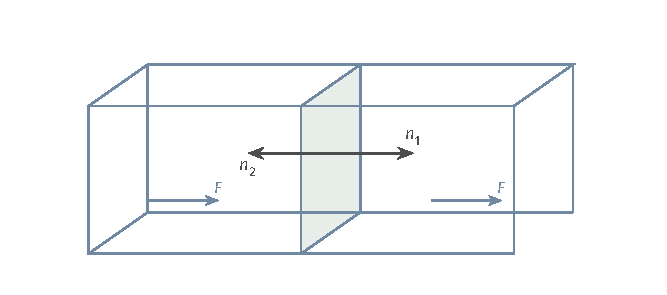
\includegraphics[width=112mm]{figures/00-shared/mathematical-preliminaries-upper/00-shared/tikz/chapter3-concept-processes/gauss-shared-face.pdf}
 \caption{两个相邻单位立方体共用绿色面，图用斜投影表示三维几何。取常场$F=(1,0,0)^\top$，共同面上两侧外法向为$n_1=(1,0,0)^\top$与$n_2=-n_1$，对应通量为$1,-1$，相加抵消。整体外向净通量也为零，与散度为零一致；一般区域的散度定理仍需要前述条件与证明。}
 \label{fig:analysis-process-gauss-shared-face}
\end{figure}

先用一个答案已知的计算核对散度定理。
\begin{example}[用散度定理核对球面面积]
设$B_R$是以原点为中心、半径$R>0$的球，边界球面取外法向。令$\bm F(\bm x)=\bm x/R$，它在整个$\mathbb R^3$上连续可微。
球面上$\bm n=\bm x/R=\bm F$，所以$\bm F^\top\bm n=1$，外向通量等于球面面积。
另一方面，$\operatorname{div}\bm F=3/R$，散度定理给出
\[
 \int_{\partial B_R}\bm F^\top\bm n\,\mathrm dS
 =\frac3R\operatorname{vol}(B_R)
 =\frac3R\cdot\frac{4\pi R^3}3=4\pi R^2.
\]
\end{example}
这里的球体积已在第~\ref{sec:classical-change-variables}节用球坐标算出；所得结果与第~\ref{sec:analysis-surface-integration}节直接参数化球面求得的面积一致。

定理要求$\bm F$在$\overline\Omega$的一个开邻域内连续可微。点源场在原点无定义，下面用它检查这一条件的作用。
\begin{example}[点源的通量]
\label{ex:analysis-point-source-flux}
在$\mathbb R^3\setminus\{\bm0\}$上取$\bm F(\bm x)=\bm x/\lVert\bm x\rVert_2^3$，记$r=\lVert\bm x\rVert_2$。由$\partial_jr=x_j/r$，
\[
 \begin{gathered}
\partial_j\Bigl(\frac{x_j}{r^3}\Bigr)=\frac1{r^3}-\frac{3x_j^2}{r^5}\\
\operatorname{div}\bm F=\frac3{r^3}-\frac{3r^2}{r^5}=0.
 \end{gathered}
\]
但在半径为$R$的球面上，外法向为$\bm x/R$，$\bm F^\top\bm n=1/R^2$，外向通量为$4\pi R^2/R^2=4\pi$。
这并不与散度定理矛盾：球体含有原点，而$\bm F$在原点无定义，定理的条件不满足。

对不含原点的球壳$R_1<r<R_2$，定理适用，左侧为零。外球面的外向通量为$4\pi$；内球面的外法向指向原点，通量为$-4\pi$；两者相加确为零。
\end{example}
所以以原点为中心的球面上的通量都是$4\pi$，与半径无关：场在原点以外处处无源，全部通量都来自原点处的点源。
静电学中，位于原点的点电荷$q$产生的电场是$\frac{q}{4\pi\varepsilon_0}\bm F$，其中$\varepsilon_0$为真空介电常数；它穿过以原点为中心的球面的通量为$q/\varepsilon_0$，这就是Gauss定律在点电荷上的形式。

\paragraph{散度是通量密度}

已证明的长方体情形，足以把散度一节的近似推导变成精确结论。
设$\bm F$在开集$U$上连续可微，$\bm a\in U$，$Q_h$是以$\bm a$为中心、边长为$h$的立方体；$h$足够小时$\overline{Q_h}\subseteq U$。由长方体上的Gauss公式，
\[
 \frac1{h^3}\int_{\partial Q_h}\bm F^\top\bm n\,\mathrm dS
 =\frac1{h^3}\int_{Q_h}\operatorname{div}\bm F\,\mathrm d\bm x.
\]
右侧是散度在$Q_h$上的平均值，它与$\operatorname{div}\bm F(\bm a)$的差不超过$\sup_{Q_h}|\operatorname{div}\bm F-\operatorname{div}\bm F(\bm a)|$。散度连续，所以$h\to0$时这个上界趋于零，平均值趋于$\operatorname{div}\bm F(\bm a)$。

这说明散度确实是“单位体积的净流出”的极限。把立方体换成以$\bm a$为中心的小球，用一般的Gauss公式可以得到同样的极限。小球的取法不依赖坐标轴，所以散度描述的是场本身的性质，不依赖坐标系的方向。

\subsection{Stokes公式与曲面的边界}

Gauss公式要求闭曲面围成空间区域。另一类问题只给一张有边界的定向曲面，要求比较曲面上的旋转累计与边界环流。
这时使用旋度在曲面法向上的分量，不需要先把曲面补成闭曲面。

\subsubsection{Stokes公式}

在$z=0$平面上取向上法向时，旋度的法向分量$(\nabla\times\bm F)^\top\bm e_3$就是Green公式中的$Q_x-P_y$。
对空间中的弯曲曲面，可以把它切成许多很小的曲面片，每片近似是一小块平面。在法向为$\bm n$的小平面片上，边界环流约等于$(\nabla\times\bm F)^\top\bm n$乘面积。
各片采用相容定向时，相邻两片的公共边被沿相反方向走过，环流相消，只剩整张曲面的边界。
用桨轮的图像说：在曲面上各处放置转轴沿法向的小桨轮，它们感受到的旋转强度按面积累加，总和等于沿曲面边缘走一圈的环流。
Stokes公式把这一关系写成精确等式，同时要求法向与边界方向相容。
\begin{theorem}[Stokes定理]
\label{thm:multivariable-stokes}
设$S\subseteq\mathbb R^3$为紧致、可定向的分片$C^2$曲面，边界由有限条分段$C^1$简单闭曲线组成。
各光滑曲面片选取连续且片间定向相容的单位法向$\bm n$，边界采用其诱导方向。
若向量场$\bm F$在$S$的开邻域内连续可微，则\term{Stokes公式}（Stokes' theorem）给出
\begin{equation}
 \oint_{\partial S}\bm F^\top\,\mathrm d\bm r
 =\int_S(\nabla\times\bm F)^\top\bm n\,\mathrm dS.
 \label{eq:multivariable-stokes}
\end{equation}
\end{theorem}
这里的“可定向”要求各曲面片能相容地选择法向，使公共边上的诱导方向相反；有折角的接缝处不要求存在唯一法向。
两侧都为标量：左侧是原向量场的边界环流，右侧是其旋度穿过曲面的通量。

在一张参数曲面片上，可以把公式归结为参数平面上的Green公式。
设参数域$D$满足Green公式的区域条件，$\bm r(u,v)$在$D$的邻域内二阶连续可微、在内部正则且一一对应，并采用$\bm r_u\times\bm r_v$确定的定向。
还要求$\partial D$的正向经$\bm r$对应曲面片边界的诱导方向，从而可以把边界路径积分放到$\partial D$上计算。
这里的$u,v$是曲面的局部参数。记
\[
 \begin{aligned}
 A(u,v)&=\bm F(\bm r(u,v))^\top\bm r_u(u,v),\\
 B(u,v)&=\bm F(\bm r(u,v))^\top\bm r_v(u,v).
 \end{aligned}
\]

先处理左侧。若$(u(t),v(t))$沿$\partial D$行进，曲面边界上对应的点是$\bm r(u(t),v(t))$，由链式法则，其速度为$\bm r_uu'(t)+\bm r_vv'(t)$。
与$\bm F$取内积，得$\bm F^\top\mathrm d\bm r=A\,\mathrm du+B\,\mathrm dv$，所以左侧等于参数平面上的路径积分$\oint_{\partial D}A\,\mathrm du+B\,\mathrm dv$。

再计算参数平面上Green公式右侧的被积函数$\partial_uB-\partial_vA$。记$\bm J_{\bm F}$为$\bm F$的Jacobian矩阵，其元素为$(\bm J_{\bm F})_{i,j}=\partial_jF_i$。由链式法则和乘积法则，
\[
 \begin{aligned}
 \partial_uB&=(\bm J_{\bm F}\bm r_u)^\top\bm r_v+\bm F^\top\bm r_{vu},\\
 \partial_vA&=(\bm J_{\bm F}\bm r_v)^\top\bm r_u+\bm F^\top\bm r_{uv},
 \end{aligned}
\]
其中$\bm J_{\bm F}$与$\bm F$在$\bm r(u,v)$处取值。$\bm r$二阶连续可微，混合偏导相等，$\bm r_{uv}=\bm r_{vu}$，所以两式相减时含二阶导数的项抵消。
又$(\bm J_{\bm F}\bm r_u)^\top\bm r_v=\bm r_v^\top\bm J_{\bm F}\bm r_u$、$(\bm J_{\bm F}\bm r_v)^\top\bm r_u=\bm r_v^\top\bm J_{\bm F}^\top\bm r_u$，于是
\[
 \partial_uB-\partial_vA=\bm r_v^\top(\bm J_{\bm F}-\bm J_{\bm F}^\top)\bm r_u.
\]

接下来把右端写成旋度。反对称矩阵$\bm W=\bm J_{\bm F}-\bm J_{\bm F}^\top$的元素为$\bm W_{i,j}=\partial_jF_i-\partial_iF_j$；逐个分量对照旋度的定义可以验证，对任意$\bm a\in\mathbb R^3$都有$\bm W\bm a=(\nabla\times\bm F)\times\bm a$。
再用混合积的轮换关系$\bm b^\top(\bm c\times\bm a)=\bm c^\top(\bm a\times\bm b)$（两边都等于以$\bm a,\bm b,\bm c$为列的行列式），取$\bm a=\bm r_u$、$\bm b=\bm r_v$、$\bm c=\nabla\times\bm F$，得到
\[
 \partial_uB-\partial_vA
 =\bigl(\operatorname{curl}\bm F\bigr)(\bm r(u,v))^\top
   (\bm r_u\times\bm r_v).
\]
右端乘$\mathrm du\,\mathrm dv$，正是曲面通量积分（式~\eqref{eq:analysis-surface-flux}）中的被积项。

$A,B$由连续可微的$\bm F$与二阶连续可微的$\bm r$及其一阶导数复合、相乘而成，在$D$的邻域内连续可微，所以参数平面上的Green公式适用；它给出该曲面片上的Stokes公式。
对有限张相容定向的曲面片，公共边的路径积分相消，只剩整张曲面的边界。
一般分片曲面的完整论证还需核对曲面覆盖及接缝条件；以上推导只说明参数片上的机制，一般定理可参考向量微积分教材\scite{math-strang1991calculus}。

\paragraph{旋度分量是环流密度}

Stokes公式也给出旋度含义的精确形式。

设$\bm F$在$\bm a$附近连续可微，$\bm n$是单位向量，$D_\rho$是以$\bm a$为圆心、半径为$\rho$、垂直于$\bm n$并取法向$\bm n$的平面圆盘。由Stokes公式，
\[
 \frac1{\pi\rho^2}\oint_{\partial D_\rho}\bm F^\top\,\mathrm d\bm r
 =\frac1{\pi\rho^2}\int_{D_\rho}(\nabla\times\bm F)^\top\bm n\,\mathrm dS,
\]
右侧是$(\nabla\times\bm F)^\top\bm n$在圆盘上的平均值。旋度连续，所以$\rho\to0$时它趋于$(\nabla\times\bm F)(\bm a)^\top\bm n$。
因此，旋度沿$\bm n$的分量就是垂直于$\bm n$的微小圆周上的环流除以所围面积的极限。这正是桨轮图像所描述的量；圆盘的取法不依赖坐标轴，所以这一含义也不依赖坐标轴的选取。

\subsubsection{跨接曲面的选择}

Stokes公式的左侧只由有向边界和边界上的向量场决定。因此，若两张满足定理条件的定向曲面具有同一有向边界，
且$\bm F$在两张曲面附近都连续可微，则两张曲面上的旋度通量相等。
计算时可以选较简单的跨接曲面，但必须核对向量场定义域，不能让替换曲面穿过场的奇点。

这一结论也可以从Gauss公式得到印证。若$\bm F$二阶连续可微，前面已由混合偏导交换证明$\operatorname{div}(\operatorname{curl}\bm F)=0$。设两张跨接曲面恰好围成一个满足Gauss公式条件的区域，且$\bm F$在该区域闭包的开邻域内二阶连续可微。
区域的外法向在一张曲面上与所选法向相同，在另一张上相反；旋度场的散度为零，所以散度定理说明两张曲面上的旋度通量之差为零。

下面用同一个场在单位圆上比较两张跨接曲面。
\begin{example}[单位圆上的圆盘与半球面]
取$\bm F=(-y/2,x/2,0)^\top$，它在整个$\mathbb R^3$上连续可微，示例~\ref{ex:analysis-rigid-rotation-curl}已算出$\nabla\times\bm F=(0,0,1)^\top$。单位圆$\{x^2+y^2=1,\ z=0\}$采用从上方看逆时针的方向。

先取向上单位圆盘$S_1$。由示例~\ref{ex:analysis-hemisphere-induced-orientation}，它的诱导方向正是这一方向；旋度的法向分量为$1$，所以
\[
 \oint_{\partial S_1}\bm F^\top\,\mathrm d\bm r
 =\iint_{S_1}1\,\mathrm dS=\pi.
\]
直接计算左侧也得到同一结果：取$\gamma(t)=(\cos t,\sin t,0)^\top$，$0\leq t\leq2\pi$，则$\bm F(\gamma(t))^\top\gamma'(t)=\tfrac12(\sin^2t+\cos^2t)=\tfrac12$，积分为$\pi$。

再取外向上半单位球面$S_2$，同一例子说明它的诱导方向与$S_1$相同。用第~\ref{sec:analysis-surface-integration}节的球面参数$(\varphi,\theta)$，$0\leq\varphi\leq\pi/2$，外法向为$\bm n=\bm x$，旋度的法向分量为$z=\cos\varphi$，面积元为$\sin\varphi\,\mathrm d\varphi\,\mathrm d\theta$，所以
\[
 \int_{S_2}(\nabla\times\bm F)^\top\bm n\,\mathrm dS
 =\int_0^{2\pi}\int_0^{\pi/2}\cos\varphi\sin\varphi\,\mathrm d\varphi\,\mathrm d\theta
 =2\pi\cdot\frac12=\pi,
\]
与圆盘上的结果相同。
\end{example}
若改用向下定向的圆盘，边界方向也必须反转，两个积分同时变号。


图~\ref{fig:analysis-process-stokes-spanning-surfaces}比较同一有向圆周的两张跨接曲面。替换曲面时，边界方向与场的定义域都要同时保留。
\begin{figure*}[!htbp]
 \centering
 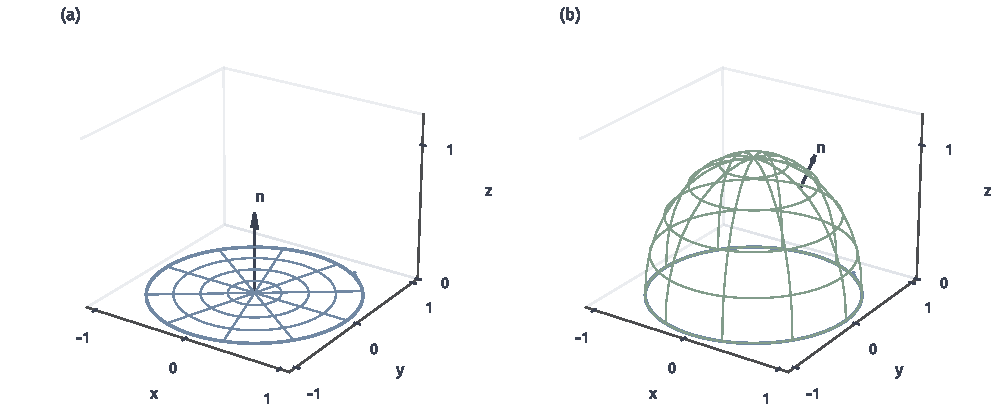
\includegraphics[width=169.0mm]{figures/00-shared/mathematical-preliminaries-upper/00-shared/matplotlib/chapter3-concept-processes/stokes-spanning-surfaces.pdf}
 \caption{(a) 向上单位圆盘；(b) 外向上半单位球面。蓝色边界均从上方看逆时针，黑箭头标记各自法向。对$F=(-y/2,x/2,0)^\top$，旋度恒为$(0,0,1)^\top$，两面上的旋度通量都为$\pi$。右面面积为$2\pi$而非$\pi$；相等的是法向分量的累计，不能把通量当成面积。}
 \label{fig:analysis-process-stokes-spanning-surfaces}
\end{figure*}

\subsection{积分分部与Green恒等式}

积分分部把导数从一个因子转移到另一个因子，同时保留边界上的贡献。

设$\Omega$满足Gauss公式的区域条件，标量函数$u$与向量场$\bm F$在$\overline\Omega$的开邻域内都是$C^1$。逐坐标使用乘积法则，得
\[
 \operatorname{div}(u\bm F)=\nabla u^\top\bm F+u\operatorname{div}\bm F.
\]
对两边积分并使用Gauss公式，移项得到
\[
 \int_\Omega u\operatorname{div}\bm F\,\mathrm dV
 =\int_{\partial\Omega}u\bm F^\top\bm n\,\mathrm dS
 -\int_\Omega\nabla u^\top\bm F\,\mathrm dV.
\]
若边界上$u=0$，或$\bm F$的法向分量为零，边界项消失；一般情况下必须保留它。取$\bm F=\nabla v$便联系到二阶微分，下面将这一情形写成正式结论。

一元分部积分（式~\eqref{eq:analysis-integration-by-parts}）把一个因子的导数转给另一个因子，并留下端点项。

设$u$在$[a,b]$上连续可微、$v$二阶连续可微，把式中的$v$换成$v'$，得到
\[
 \int_a^bu\,v''\,\mathrm dx
 =u(b)v'(b)\cdot(+1)+u(a)v'(a)\cdot(-1)-\int_a^bu'v'\,\mathrm dx.
\]
这里把端点项$[uv']_a^b$拆开写：区间在右端点的外法向是$+1$，在左端点是$-1$。

推广到多元情形时，各项依次对应：二阶导数$v''$换成$\Delta v$，一阶导数的乘积$u'v'$换成梯度的内积$\nabla u^\top\nabla v$，两个端点换成边界曲面，“$v'$乘外法向$\pm1$”换成$\nabla v^\top\bm n$，即$v$沿外法向的方向导数。
对乘积向量场$u\nabla v$使用散度定理，就得到这一推广。
\begin{theorem}[多元分部积分]
\label{thm:multivariable-integration-by-parts}
设$\Omega\subseteq\mathbb R^3$满足上述Gauss公式的区域条件。
若标量函数$u$在$\overline\Omega$的开邻域内连续可微，$v$在同一邻域内二阶连续可微，则
\[
 \int_\Omega u\Delta v\,\mathrm d\bm x
 =\int_{\partial\Omega}u\nabla v^\top\bm n\,\mathrm dS
  -\int_\Omega\nabla u^\top\nabla v\,\mathrm d\bm x.
\]
\end{theorem}
\begin{proof}
向量场$\bm F=u\nabla v$的第$j$个分量是$u\,\partial_jv$，它连续可微。由一元乘积法则，
$\partial_j(u\,\partial_jv)=\partial_ju\,\partial_jv+u\,\partial_j^2v$，对$j$求和得到
\[
 \operatorname{div}(u\nabla v)
 =\nabla u^\top\nabla v+u\Delta v.
\]
将它代入Gauss公式，再把$\nabla u^\top\nabla v$的区域积分移到等式另一侧，即得结论。
\end{proof}
对满足Green公式条件的平面区域，同样的证明改用平面通量公式（定理~\ref{thm:multivariable-planar-flux}）即可，边界面积元素相应换成弧长元素。
这一公式把$v$的二阶导数转移为$u$与$v$的一阶导数，同时保留法向边界项；该项是否为零，必须由具体边界条件决定。

取$u=1$，公式化为$\int_\Omega\Delta v\,\mathrm d\bm x=\int_{\partial\Omega}\nabla v^\top\bm n\,\mathrm dS$，也就是对梯度场$\nabla v$使用散度定理。下面在球上核对这一特例。
\begin{example}[球上平方范数的Laplace积分]
取以原点为中心、半径为$R$的球$B_R$和$v(\bm x)=\lVert\bm x\rVert_2^2$。
左侧：$\Delta v=6$，所以$\int_{B_R}\Delta v\,\mathrm d\bm x=6\operatorname{vol}(B_R)=6\cdot\frac{4\pi R^3}3=8\pi R^3$。
右侧：球面上$\nabla v=2\bm x$，外法向$\bm n=\bm x/R$，故$\nabla v^\top\bm n=2\lVert\bm x\rVert_2^2/R=2R$，积分为$2R\cdot4\pi R^2=8\pi R^3$。两侧相等。
\end{example}

边界项为零时，公式可以给出结构性的结论。下面用它说明Laplace方程的解由边界值唯一确定。
\begin{example}[Laplace方程的解由边界值决定]
设$\Omega$满足Gauss公式的区域条件，$w$在$\overline\Omega$的开邻域内二阶连续可微，在$\Omega$内$\Delta w=0$，在$\partial\Omega$上$w=0$。
在定理~\ref{thm:multivariable-integration-by-parts}中取$u=v=w$。左侧被积函数$w\Delta w$为零；边界项的被积函数含因子$w$，也为零。于是
\[
 \int_\Omega\lVert\nabla w\rVert_2^2\,\mathrm d\bm x=0.
\]
被积函数连续且非负；若它在某点为正，则在该点的一个邻域内为正，积分也为正。所以在开集$\Omega$上$\nabla w$恒为零。
$\Omega$是连通的开区域，所以$w$在$\Omega$上为常数；再由$w$在$\overline\Omega$上连续且在边界上为零，得$w\equiv0$。

现在设$v_1,v_2$都在$\overline\Omega$的开邻域内二阶连续可微，在$\Omega$内满足$\Delta v_1=\Delta v_2=0$，在$\partial\Omega$上取值相同。差$w=v_1-v_2$满足上面的全部条件，所以$v_1=v_2$。
\end{example}
按热传导的解释，稳定的温度分布由边界温度唯一决定。

若$u,v$都为$C^2$函数，交换分部积分公式中的$u,v$，再将两式相减，梯度内积项抵消，得到Green第二恒等式：
\[
 \int_\Omega (u\Delta v-v\Delta u)\,\mathrm d\bm x
 =\int_{\partial\Omega}(u\nabla v-v\nabla u)^\top\bm n\,\mathrm dS.
\]
前面的分部积分公式也称Green第一恒等式。两式都要求同样的区域规则性和边界定向；第二式通过交换两个函数，显示边界项怎样控制Laplace作用在积分配对中的交换。

\paragraph{积分公式的比较}

本节各公式回答的都是同一类问题：导数在内部的积分与边界积分之间的关系。推导方式也相同：在小块上建立局部关系，再利用相容方向让内部边界相消。
它们的内部对象、边界对象和方向条件则各不相同。下表把一元基本定理与路径积分基本定理也列在一起，二者以区间或路径的两个端点为边界。
\begin{center}
\begin{tabular}{lll}
\toprule
公式 & 内部积分 & 边界积分\\
\midrule
一元基本定理 & 区间上的$f'$ & 端点值之差$f(b)-f(a)$\\
路径积分基本定理 & 路径上$\nabla\phi$的切向积分 & 端点值之差\\
Green环流形式 & 平面区域的$Q_x-P_y$ & 正向路径的切向积分\\
Gauss & 空间区域的散度 & 闭曲面的外向通量\\
Stokes & 定向曲面的旋度通量 & 诱导方向的路径环流\\
\bottomrule
\end{tabular}
\end{center}
对向上定向的平面曲面，Stokes公式还原为Green公式的环流形式；Green公式的通量形式则是二维的散度公式。
普通标量函数的区域积分不自动具有边界表达：要使用这些公式，须先找到满足条件的向量场，使其散度或旋度的相应分量等于被积函数。示例~\ref{ex:analysis-green-area-formula}的面积公式就是先选出满足$Q_x-P_y\equiv1$的场。

Stokes公式还解释了第~\ref{sec:multivariable-potential-path-independence}节中势函数的存在为何与定义域有关。设$\bm F$在开集$U\subseteq\mathbb R^3$上连续可微且$\nabla\times\bm F=\bm0$。若一条闭路径是$U$内某张满足定理条件的定向曲面的有向边界，则该闭路径上的环流等于旋度的通量，也就是零。
在星形域中，闭路径上各点与中心点之间的线段扫出一张锥面，它整个落在定义域内，不会碰到场的奇点；这与那里在星形域上构造势函数的结论一致。
穿孔平面上绕原点的单位圆则不同：在平面内，以它为边界的区域只能是单位圆盘，必然包含原点，而场在原点无定义；所以局部条件$Q_x-P_y=0$并不排除$2\pi$的环流（示例~\ref{ex:analysis-annulus-vortex-green}）。

各公式均使用本章的经典积分。连续可微性、分片规则边界与定向是这里的经典公式所需的条件，并不是另换一种积分定义。
尤其要核对向量场是否在整个积分对象附近都有定义：穿孔平面上的涡旋场在原点无定义，不能把包含原点的圆盘直接代入Green公式；点源场也不能直接用于包含原点的球体（示例~\ref{ex:analysis-point-source-flux}）。
区域积分中可以忽略的边界，对边界积分却正是累计对象。因此必须指定场在边界处的实际取值，并检查其连续可微的延拓，不能只凭区域内部的积分值推断边界积分。
如果要降低导数或边界的规则性，还须另外建立弱导数、边界迹及相应的积分公式；不能沿用当前公式而省去这些条件。

\FloatBarrier


\FloatBarrier
\section{本章小结}
\label{sec:multivariable-summary}

区域积分把密度累计成总量；连续性和规则的区域边界保证可以逐个坐标切片计算，Jacobian行列式的绝对值给出坐标变换下的体积缩放。第一类路径积分与曲面积分按弧长和面积累计，不依赖方向；第二类路径积分计算做功，第二类曲面积分计算通量，二者都随方向反转而变号。

保守场的功只取决于端点。交叉偏导相等在星形区域上保证势函数存在，在有孔的区域上则不够。散度是单位体积的净流出，旋度是单位面积的环流；Green、Gauss和Stokes公式将内部的散度或旋度累计与边界上的通量或环流联系起来。使用这些公式时，应检查域内奇点、场的光滑性、完整边界及其定向。

